\documentclass[twoside]{book}

% Packages required by doxygen
\usepackage{fixltx2e}
\usepackage{calc}
\usepackage{doxygen}
\usepackage[export]{adjustbox} % also loads graphicx
\usepackage{graphicx}
\usepackage[utf8]{inputenc}
\usepackage{makeidx}
\usepackage{multicol}
\usepackage{multirow}
\PassOptionsToPackage{warn}{textcomp}
\usepackage{textcomp}
\usepackage[nointegrals]{wasysym}
\usepackage[table]{xcolor}

% Font selection
\usepackage[T1]{fontenc}
\usepackage[scaled=.90]{helvet}
\usepackage{courier}
\usepackage{amssymb}
\usepackage{sectsty}
\renewcommand{\familydefault}{\sfdefault}
\allsectionsfont{%
  \fontseries{bc}\selectfont%
  \color{darkgray}%
}
\renewcommand{\DoxyLabelFont}{%
  \fontseries{bc}\selectfont%
  \color{darkgray}%
}
\newcommand{\+}{\discretionary{\mbox{\scriptsize$\hookleftarrow$}}{}{}}

% Page & text layout
\usepackage{geometry}
\geometry{%
  a4paper,%
  top=2.5cm,%
  bottom=2.5cm,%
  left=2.5cm,%
  right=2.5cm%
}
\tolerance=750
\hfuzz=15pt
\hbadness=750
\setlength{\emergencystretch}{15pt}
\setlength{\parindent}{0cm}
\setlength{\parskip}{0.2cm}
\makeatletter
\renewcommand{\paragraph}{%
  \@startsection{paragraph}{4}{0ex}{-1.0ex}{1.0ex}{%
    \normalfont\normalsize\bfseries\SS@parafont%
  }%
}
\renewcommand{\subparagraph}{%
  \@startsection{subparagraph}{5}{0ex}{-1.0ex}{1.0ex}{%
    \normalfont\normalsize\bfseries\SS@subparafont%
  }%
}
\makeatother

% Headers & footers
\usepackage{fancyhdr}
\pagestyle{fancyplain}
\fancyhead[LE]{\fancyplain{}{\bfseries\thepage}}
\fancyhead[CE]{\fancyplain{}{}}
\fancyhead[RE]{\fancyplain{}{\bfseries\leftmark}}
\fancyhead[LO]{\fancyplain{}{\bfseries\rightmark}}
\fancyhead[CO]{\fancyplain{}{}}
\fancyhead[RO]{\fancyplain{}{\bfseries\thepage}}
\fancyfoot[LE]{\fancyplain{}{}}
\fancyfoot[CE]{\fancyplain{}{}}
\fancyfoot[RE]{\fancyplain{}{\bfseries\scriptsize Generated on Wed Nov 11 2015 00\+:22\+:20 for Fillwave by Doxygen }}
\fancyfoot[LO]{\fancyplain{}{\bfseries\scriptsize Generated on Wed Nov 11 2015 00\+:22\+:20 for Fillwave by Doxygen }}
\fancyfoot[CO]{\fancyplain{}{}}
\fancyfoot[RO]{\fancyplain{}{}}
\renewcommand{\footrulewidth}{0.4pt}
\renewcommand{\chaptermark}[1]{%
  \markboth{#1}{}%
}
\renewcommand{\sectionmark}[1]{%
  \markright{\thesection\ #1}%
}

% Indices & bibliography
\usepackage{natbib}
\usepackage[titles]{tocloft}
\setcounter{tocdepth}{3}
\setcounter{secnumdepth}{5}
\makeindex

% Hyperlinks (required, but should be loaded last)
\usepackage{ifpdf}
\ifpdf
  \usepackage[pdftex,pagebackref=true]{hyperref}
\else
  \usepackage[ps2pdf,pagebackref=true]{hyperref}
\fi
\hypersetup{%
  colorlinks=true,%
  linkcolor=blue,%
  citecolor=blue,%
  unicode%
}

% Custom commands
\newcommand{\clearemptydoublepage}{%
  \newpage{\pagestyle{empty}\cleardoublepage}%
}


%===== C O N T E N T S =====

\begin{document}

% Titlepage & ToC
\hypersetup{pageanchor=false,
             bookmarks=true,
             bookmarksnumbered=true,
             pdfencoding=unicode
            }
\pagenumbering{roman}
\begin{titlepage}
\vspace*{7cm}
\begin{center}%
{\Large Fillwave \\[1ex]\large 2.\+1.\+3 }\\
\vspace*{1cm}
{\large Generated by Doxygen 1.8.9.1}\\
\vspace*{0.5cm}
{\small Wed Nov 11 2015 00:22:20}\\
\end{center}
\end{titlepage}
\clearemptydoublepage
\tableofcontents
\clearemptydoublepage
\pagenumbering{arabic}
\hypersetup{pageanchor=true}

%--- Begin generated contents ---
\chapter{Fillwave graphics engine for c++11.}
\label{index}\hypertarget{index}{}\subsection*{{\bfseries Requirements}}


\begin{DoxyItemize}
\item P\+C with Open\+G\+L 3.\+3+ and G\+L\+S\+L 330+ support.
\item Android with Open\+G\+L 3.\+0+, G\+L\+S\+L E\+S 300+ support. (A\+P\+I $>$ 18, Rev. $>$ 4.\+3)
\end{DoxyItemize}

\subsection*{{\bfseries Ubuntu (Debian)\+:}}

\subsubsection*{1. Install all dependencies\+:}


\begin{DoxyPre}
{\ttfamily 
sudo apt-get install libfreetype6 libfreetype6-dev libassimp3 libassimp-dev libglm-dev libglm libx11-dev libglu-dev
}
\end{DoxyPre}


\subsubsection*{2.\+a) Install from the package directly ...}


\begin{DoxyItemize}
\item \href{http://filipwasil.bitbucket.org/downloads/libfillwave-1.9.7-Linux.deb}{\tt http\+://filipwasil.\+bitbucket.\+org/downloads/libfillwave-\/1.\+9.\+7-\/\+Linux.\+deb}
\item \href{http://filipwasil.bitbucket.org/downloads/libfillwave-dev-1.9.7-Linux.deb}{\tt http\+://filipwasil.\+bitbucket.\+org/downloads/libfillwave-\/dev-\/1.\+9.\+7-\/\+Linux.\+deb}
\end{DoxyItemize}

\subsubsection*{2.\+b) ... or add fillwave to software sources\+:}


\begin{DoxyPre}
{\ttfamily 
deb \href{http://filipwasil.bitbucket.org/downloads}{\tt http://filipwasil.bitbucket.org/downloads} ./
#deb-src \href{http://filipwasil.bitbucket.org/downloads}{\tt http://filipwasil.bitbucket.org/downloads} ./
}
\end{DoxyPre}


\subsubsection*{3. Update and install\+:}


\begin{DoxyPre}{\ttfamily sudo apt-get update
}\end{DoxyPre}
  
\begin{DoxyPre}{\ttfamily sudo apt-get install sudo apt-get install libfillwave libfillwave-dev fillwave-examples
}\end{DoxyPre}
 

\subsection*{{\bfseries Fedora (Red hat)\+:}}

\subsubsection*{1. Install all dependencies\+:}


\begin{DoxyPre}
{\ttfamily 
sudo yum install glm-devel.x86\_64 glm.x86\_64 assimp.x86\_64 assimp-devel.x86\_64 glew.x86\_64 glew-devel.x86\_64 freetype-devel.x86\_64 freetype.x86\_64
}
\end{DoxyPre}


\subsubsection*{2. Copy \href{downloads/fillwave.repo}{\tt fillwave.\+repo} file in Your {\bfseries /etc/yum.repos.\+d/}, update and install.}


\begin{DoxyPre}{\ttfamily sudo yum update
}\end{DoxyPre}
  
\begin{DoxyPre}{\ttfamily sudo yum install sudo apt-get install libfillwave libfillwave-dev fillwave-examples
}\end{DoxyPre}
 

\subsection*{{\bfseries G\+L\+F\+W3 for context creation on P\+C}}

The easiest way to start playing with Fillwave engine on P\+C is to create context with G\+L\+F\+W3 and use examples provided. G\+L\+F\+W3 is in default repositries under \href{http://www.ubuntu.com/}{\tt Ubuntu} 14.\+10+. In case of older system just add following lines to /etc/apt/sources.list\+:

 
\begin{DoxyPre}
{\ttfamily 
deb \href{http://ppa.launchpad.net/keithw/glfw3/ubuntu}{\tt http://ppa.launchpad.net/keithw/glfw3/ubuntu} trusty main
deb-src \href{http://ppa.launchpad.net/keithw/glfw3/ubuntu}{\tt http://ppa.launchpad.net/keithw/glfw3/ubuntu} trusty main
}
\end{DoxyPre}
 \subsubsection*{{\bfseries G\+L\+F\+W3 installation}}

  
\begin{DoxyPre}
{\ttfamily 
sudo apt-get install libglfw3
}
\end{DoxyPre}




\subsection*{{\bfseries Android}}

 

 You can develop Android with pure native activity, or regular activity with J\+N\+I wrapper.



\subsubsection*{{\bfseries Java Activity with J\+N\+I}}




\begin{DoxyItemize}
\item \href{https://github.com/filipwasil/fillwave-android-jni-lib}{\tt https\+://github.\+com/filipwasil/fillwave-\/android-\/jni-\/lib}
\item \href{https://github.com/filipwasil/fillwave-android-activity.git}{\tt https\+://github.\+com/filipwasil/fillwave-\/android-\/activity.\+git}
\end{DoxyItemize}

\subsubsection*{{\bfseries Native Activity}}




\begin{DoxyItemize}
\item \href{https://github.com/filipwasil/fillwave-android-activity-native}{\tt https\+://github.\+com/filipwasil/fillwave-\/android-\/activity-\/native}
\end{DoxyItemize}

\subsubsection*{{\bfseries Libraries used}}




\begin{DoxyItemize}
\item \href{http://www.glfw.org}{\tt glfw} released under \href{v}{\tt zlib/libpng (a B\+S\+D-\/like) license} 
\item \href{https://github.com/omniavinco/glew-cmake}{\tt glew } released under \href{http://glew.sourceforge.net/glew.txt}{\tt Modified B\+S\+D license}, the\href{http://glew.sourceforge.net/mesa.txt}{\tt Mesa 3-\/\+D License (M\+I\+T License)} and the \href{http://glew.sourceforge.net/khronos.txt}{\tt the Khronos License (M\+I\+T License)} 
\item \href{http://assimp.sourceforge.net/}{\tt assimp} released under \href{http://assimp.sourceforge.net/main_license.html}{\tt 3-\/clause B\+S\+D license} 
\item \href{http://glm.g-truc.net}{\tt glm} released under \href{http://glm.g-truc.net/copying.txt}{\tt M\+I\+T license}  
\item \href{http://www.freetype.org}{\tt freetype} released under \href{http://git.savannah.gnu.org/cgit/freetype/freetype2.git/tree/docs/FTL.TXT}{\tt Free\+Type License} 
\item \href{https://github.com/nothings/stb}{\tt stb library} released under \href{https://github.com/nothings/stb/blob/master/README.md#whats-the-license}{\tt Public Domain License} 
\item \href{https://github.com/poole/lanyon}{\tt Lanyon} page template released under \href{https://github.com/poole/lanyon/blob/master/LICENSE.md}{\tt M\+I\+T license} 
\end{DoxyItemize}
\chapter{Hierarchical Index}
\section{Class Hierarchy}
This inheritance list is sorted roughly, but not completely, alphabetically\+:\begin{DoxyCompactList}
\item \contentsline{section}{fillwave\+:\+:animation\+:\+:Animation}{\pageref{classfillwave_1_1animation_1_1Animation}}{}
\item \contentsline{section}{fillwave\+:\+:manager\+:\+:Assimp\+Node}{\pageref{classfillwave_1_1manager_1_1AssimpNode}}{}
\item \contentsline{section}{fillwave\+:\+:core\+:\+:Attribute}{\pageref{classfillwave_1_1core_1_1Attribute}}{}
\item \contentsline{section}{fillwave\+:\+:common\+:\+:Blending}{\pageref{structfillwave_1_1common_1_1Blending}}{}
\item \contentsline{section}{fillwave\+:\+:manager\+:\+:Bone\+Manager}{\pageref{classfillwave_1_1manager_1_1BoneManager}}{}
\item \contentsline{section}{fillwave\+:\+:manager\+:\+:Buffer\+Manager}{\pageref{classfillwave_1_1manager_1_1BufferManager}}{}
\item \contentsline{section}{fillwave\+:\+:particles\+:\+:Builder\+Emiter}{\pageref{classfillwave_1_1particles_1_1BuilderEmiter}}{}
\item \contentsline{section}{fillwave\+:\+:models\+:\+:Builder\+Model}{\pageref{classfillwave_1_1models_1_1BuilderModel}}{}
\begin{DoxyCompactList}
\item \contentsline{section}{fillwave\+:\+:models\+:\+:Builder\+Model\+External\+Maps}{\pageref{classfillwave_1_1models_1_1BuilderModelExternalMaps}}{}
\item \contentsline{section}{fillwave\+:\+:models\+:\+:Builder\+Model\+Manual}{\pageref{classfillwave_1_1models_1_1BuilderModelManual}}{}
\end{DoxyCompactList}
\item \contentsline{section}{fillwave\+:\+:actions\+:\+:Callback}{\pageref{classfillwave_1_1actions_1_1Callback}}{}
\begin{DoxyCompactList}
\item \contentsline{section}{fillwave\+:\+:actions\+:\+:Engine\+Callback}{\pageref{classfillwave_1_1actions_1_1EngineCallback}}{}
\begin{DoxyCompactList}
\item \contentsline{section}{fillwave\+:\+:actions\+:\+:F\+P\+S\+Callback}{\pageref{classfillwave_1_1actions_1_1FPSCallback}}{}
\end{DoxyCompactList}
\item \contentsline{section}{fillwave\+:\+:actions\+:\+:Item\+Callback}{\pageref{classfillwave_1_1actions_1_1ItemCallback}}{}
\begin{DoxyCompactList}
\item \contentsline{section}{fillwave\+:\+:actions\+:\+:Loop\+Callback}{\pageref{classfillwave_1_1actions_1_1LoopCallback}}{}
\item \contentsline{section}{fillwave\+:\+:actions\+:\+:Sequence\+Callback}{\pageref{classfillwave_1_1actions_1_1SequenceCallback}}{}
\item \contentsline{section}{fillwave\+:\+:actions\+:\+:Timed\+Callback}{\pageref{classfillwave_1_1actions_1_1TimedCallback}}{}
\begin{DoxyCompactList}
\item \contentsline{section}{fillwave\+:\+:actions\+:\+:Timed\+Bone\+Update\+Callback}{\pageref{classfillwave_1_1actions_1_1TimedBoneUpdateCallback}}{}
\item \contentsline{section}{fillwave\+:\+:actions\+:\+:Timed\+Color\+Callback}{\pageref{classfillwave_1_1actions_1_1TimedColorCallback}}{}
\item \contentsline{section}{fillwave\+:\+:actions\+:\+:Timed\+Emiter\+Update\+Callback}{\pageref{classfillwave_1_1actions_1_1TimedEmiterUpdateCallback}}{}
\item \contentsline{section}{fillwave\+:\+:actions\+:\+:Timed\+Move\+Callback}{\pageref{classfillwave_1_1actions_1_1TimedMoveCallback}}{}
\item \contentsline{section}{fillwave\+:\+:actions\+:\+:Timed\+Rotate\+Callback}{\pageref{classfillwave_1_1actions_1_1TimedRotateCallback}}{}
\item \contentsline{section}{fillwave\+:\+:actions\+:\+:Timed\+Scale\+Callback}{\pageref{classfillwave_1_1actions_1_1TimedScaleCallback}}{}
\end{DoxyCompactList}
\end{DoxyCompactList}
\end{DoxyCompactList}
\item \contentsline{section}{fillwave\+:\+:animation\+:\+:Channel}{\pageref{classfillwave_1_1animation_1_1Channel}}{}
\item \contentsline{section}{fillwave\+:\+:actions\+:\+:Character\+Event\+Data}{\pageref{structfillwave_1_1actions_1_1CharacterEventData}}{}
\item \contentsline{section}{fillwave\+:\+:actions\+:\+:Character\+Mods\+Event\+Data}{\pageref{structfillwave_1_1actions_1_1CharacterModsEventData}}{}
\item \contentsline{section}{fillwave\+:\+:core\+:\+:Conditional\+Render}{\pageref{classfillwave_1_1core_1_1ConditionalRender}}{}
\item \contentsline{section}{fillwave\+:\+:space\+:\+:Culling\+Box}{\pageref{structfillwave_1_1space_1_1CullingBox}}{}
\item \contentsline{section}{fillwave\+:\+:actions\+:\+:Cursor\+Enter\+Event\+Data}{\pageref{structfillwave_1_1actions_1_1CursorEnterEventData}}{}
\item \contentsline{section}{fillwave\+:\+:actions\+:\+:Cursor\+Position\+Event\+Data}{\pageref{structfillwave_1_1actions_1_1CursorPositionEventData}}{}
\item \contentsline{section}{fillwave\+:\+:effects\+:\+:Effect}{\pageref{classfillwave_1_1effects_1_1Effect}}{}
\begin{DoxyCompactList}
\item \contentsline{section}{fillwave\+:\+:effects\+:\+:Boost\+Color}{\pageref{classfillwave_1_1effects_1_1BoostColor}}{}
\item \contentsline{section}{fillwave\+:\+:effects\+:\+:Clockwise\+Draw\+Effect}{\pageref{classfillwave_1_1effects_1_1ClockwiseDrawEffect}}{}
\item \contentsline{section}{fillwave\+:\+:effects\+:\+:Fog}{\pageref{classfillwave_1_1effects_1_1Fog}}{}
\item \contentsline{section}{fillwave\+:\+:effects\+:\+:Painter}{\pageref{classfillwave_1_1effects_1_1Painter}}{}
\item \contentsline{section}{fillwave\+:\+:effects\+:\+:Texture\+Only}{\pageref{classfillwave_1_1effects_1_1TextureOnly}}{}
\end{DoxyCompactList}
\item \contentsline{section}{fillwave\+:\+:Engine}{\pageref{classfillwave_1_1Engine}}{}
\item \contentsline{section}{fillwave\+:\+:Engine\+:\+:Engine\+Impl}{\pageref{structfillwave_1_1Engine_1_1EngineImpl}}{}
\item \contentsline{section}{fillwave\+:\+:actions\+:\+:Event\+Type}{\pageref{classfillwave_1_1actions_1_1EventType}}{}
\begin{DoxyCompactList}
\item \contentsline{section}{fillwave\+:\+:actions\+:\+:Event$<$ Character\+Event\+Data $>$}{\pageref{classfillwave_1_1actions_1_1Event}}{}
\begin{DoxyCompactList}
\item \contentsline{section}{fillwave\+:\+:actions\+:\+:Character\+Event}{\pageref{classfillwave_1_1actions_1_1CharacterEvent}}{}
\end{DoxyCompactList}
\item \contentsline{section}{fillwave\+:\+:actions\+:\+:Event$<$ Character\+Mods\+Event\+Data $>$}{\pageref{classfillwave_1_1actions_1_1Event}}{}
\begin{DoxyCompactList}
\item \contentsline{section}{fillwave\+:\+:actions\+:\+:Character\+Mods\+Event}{\pageref{classfillwave_1_1actions_1_1CharacterModsEvent}}{}
\end{DoxyCompactList}
\item \contentsline{section}{fillwave\+:\+:actions\+:\+:Event$<$ Cursor\+Enter\+Event\+Data $>$}{\pageref{classfillwave_1_1actions_1_1Event}}{}
\begin{DoxyCompactList}
\item \contentsline{section}{fillwave\+:\+:actions\+:\+:Cursor\+Enter\+Event}{\pageref{classfillwave_1_1actions_1_1CursorEnterEvent}}{}
\end{DoxyCompactList}
\item \contentsline{section}{fillwave\+:\+:actions\+:\+:Event$<$ Cursor\+Position\+Event\+Data $>$}{\pageref{classfillwave_1_1actions_1_1Event}}{}
\begin{DoxyCompactList}
\item \contentsline{section}{fillwave\+:\+:actions\+:\+:Cursor\+Position\+Event}{\pageref{classfillwave_1_1actions_1_1CursorPositionEvent}}{}
\end{DoxyCompactList}
\item \contentsline{section}{fillwave\+:\+:actions\+:\+:Event$<$ Keyboard\+Event\+Data $>$}{\pageref{classfillwave_1_1actions_1_1Event}}{}
\begin{DoxyCompactList}
\item \contentsline{section}{fillwave\+:\+:actions\+:\+:Keyboard\+Event}{\pageref{classfillwave_1_1actions_1_1KeyboardEvent}}{}
\end{DoxyCompactList}
\item \contentsline{section}{fillwave\+:\+:actions\+:\+:Event$<$ Mouse\+Button\+Event\+Data $>$}{\pageref{classfillwave_1_1actions_1_1Event}}{}
\begin{DoxyCompactList}
\item \contentsline{section}{fillwave\+:\+:actions\+:\+:Mouse\+Button\+Event}{\pageref{classfillwave_1_1actions_1_1MouseButtonEvent}}{}
\end{DoxyCompactList}
\item \contentsline{section}{fillwave\+:\+:actions\+:\+:Event$<$ Scroll\+Event\+Data $>$}{\pageref{classfillwave_1_1actions_1_1Event}}{}
\begin{DoxyCompactList}
\item \contentsline{section}{fillwave\+:\+:actions\+:\+:Scroll\+Event}{\pageref{classfillwave_1_1actions_1_1ScrollEvent}}{}
\end{DoxyCompactList}
\item \contentsline{section}{fillwave\+:\+:actions\+:\+:Event$<$ Time\+Event\+Data $>$}{\pageref{classfillwave_1_1actions_1_1Event}}{}
\begin{DoxyCompactList}
\item \contentsline{section}{fillwave\+:\+:actions\+:\+:Time\+Event}{\pageref{classfillwave_1_1actions_1_1TimeEvent}}{}
\end{DoxyCompactList}
\item \contentsline{section}{fillwave\+:\+:actions\+:\+:Event$<$ Touch\+Event\+Data $>$}{\pageref{classfillwave_1_1actions_1_1Event}}{}
\begin{DoxyCompactList}
\item \contentsline{section}{fillwave\+:\+:actions\+:\+:Touch\+Event}{\pageref{classfillwave_1_1actions_1_1TouchEvent}}{}
\end{DoxyCompactList}
\item \contentsline{section}{fillwave\+:\+:actions\+:\+:Event$<$ T $>$}{\pageref{classfillwave_1_1actions_1_1Event}}{}
\end{DoxyCompactList}
\item \contentsline{section}{fillwave\+:\+:core\+:\+:Face\+Basic}{\pageref{structfillwave_1_1core_1_1FaceBasic}}{}
\item \contentsline{section}{fillwave\+:\+:core\+:\+:Fence}{\pageref{classfillwave_1_1core_1_1Fence}}{}
\item \contentsline{section}{fillwave\+:\+:loader\+:\+:File\+Loader}{\pageref{classfillwave_1_1loader_1_1FileLoader}}{}
\item \contentsline{section}{fillwave\+:\+:common\+:\+:Finishable}{\pageref{classfillwave_1_1common_1_1Finishable}}{}
\begin{DoxyCompactList}
\item \contentsline{section}{fillwave\+:\+:actions\+:\+:Item\+Callback}{\pageref{classfillwave_1_1actions_1_1ItemCallback}}{}
\item \contentsline{section}{fillwave\+:\+:common\+:\+:Post\+Processing\+Pass}{\pageref{classfillwave_1_1common_1_1PostProcessingPass}}{}
\item \contentsline{section}{fillwave\+:\+:particles\+:\+:Impostor}{\pageref{classfillwave_1_1particles_1_1Impostor}}{}
\begin{DoxyCompactList}
\item \contentsline{section}{fillwave\+:\+:particles\+:\+:Cursor}{\pageref{classfillwave_1_1particles_1_1Cursor}}{}
\end{DoxyCompactList}
\end{DoxyCompactList}
\item \contentsline{section}{fillwave\+:\+:loader\+:\+:Font\+Loader}{\pageref{classfillwave_1_1loader_1_1FontLoader}}{}
\item \contentsline{section}{fillwave\+:\+:core\+:\+:G\+L\+Object}{\pageref{classfillwave_1_1core_1_1GLObject}}{}
\begin{DoxyCompactList}
\item \contentsline{section}{fillwave\+:\+:core\+:\+:Buffer}{\pageref{classfillwave_1_1core_1_1Buffer}}{}
\begin{DoxyCompactList}
\item \contentsline{section}{fillwave\+:\+:core\+:\+:Index\+Buffer}{\pageref{classfillwave_1_1core_1_1IndexBuffer}}{}
\begin{DoxyCompactList}
\item \contentsline{section}{fillwave\+:\+:core\+:\+:Index\+Buffer\+Basic}{\pageref{classfillwave_1_1core_1_1IndexBufferBasic}}{}
\item \contentsline{section}{fillwave\+:\+:core\+:\+:Index\+Buffer\+Particles}{\pageref{classfillwave_1_1core_1_1IndexBufferParticles}}{}
\end{DoxyCompactList}
\item \contentsline{section}{fillwave\+:\+:core\+:\+:Pixel\+Buffer}{\pageref{classfillwave_1_1core_1_1PixelBuffer}}{}
\item \contentsline{section}{fillwave\+:\+:core\+:\+:Uniform\+Buffer}{\pageref{classfillwave_1_1core_1_1UniformBuffer}}{}
\item \contentsline{section}{fillwave\+:\+:core\+:\+:Vertex\+Buffer$<$ T $>$}{\pageref{classfillwave_1_1core_1_1VertexBuffer}}{}
\item \contentsline{section}{fillwave\+:\+:core\+:\+:Vertex\+Buffer$<$ G\+Lfloat $>$}{\pageref{classfillwave_1_1core_1_1VertexBuffer}}{}
\begin{DoxyCompactList}
\item \contentsline{section}{fillwave\+:\+:core\+:\+:Vertex\+Buffer\+Float}{\pageref{classfillwave_1_1core_1_1VertexBufferFloat}}{}
\end{DoxyCompactList}
\item \contentsline{section}{fillwave\+:\+:core\+:\+:Vertex\+Buffer$<$ Vertex\+Basic $>$}{\pageref{classfillwave_1_1core_1_1VertexBuffer}}{}
\begin{DoxyCompactList}
\item \contentsline{section}{fillwave\+:\+:core\+:\+:Vertex\+Buffer\+Basic}{\pageref{classfillwave_1_1core_1_1VertexBufferBasic}}{}
\end{DoxyCompactList}
\item \contentsline{section}{fillwave\+:\+:core\+:\+:Vertex\+Buffer$<$ Vertex\+Debug $>$}{\pageref{classfillwave_1_1core_1_1VertexBuffer}}{}
\begin{DoxyCompactList}
\item \contentsline{section}{fillwave\+:\+:core\+:\+:Vertex\+Buffer\+Debug}{\pageref{classfillwave_1_1core_1_1VertexBufferDebug}}{}
\end{DoxyCompactList}
\item \contentsline{section}{fillwave\+:\+:core\+:\+:Vertex\+Buffer$<$ Vertex\+Particle $>$}{\pageref{classfillwave_1_1core_1_1VertexBuffer}}{}
\begin{DoxyCompactList}
\item \contentsline{section}{fillwave\+:\+:core\+:\+:Vertex\+Buffer\+Particles}{\pageref{classfillwave_1_1core_1_1VertexBufferParticles}}{}
\end{DoxyCompactList}
\item \contentsline{section}{fillwave\+:\+:core\+:\+:Vertex\+Buffer$<$ Vertex\+Particle\+G\+P\+U $>$}{\pageref{classfillwave_1_1core_1_1VertexBuffer}}{}
\begin{DoxyCompactList}
\item \contentsline{section}{fillwave\+:\+:core\+:\+:Vertex\+Buffer\+Particles\+G\+P\+U}{\pageref{classfillwave_1_1core_1_1VertexBufferParticlesGPU}}{}
\end{DoxyCompactList}
\item \contentsline{section}{fillwave\+:\+:core\+:\+:Vertex\+Buffer$<$ Vertex\+Position $>$}{\pageref{classfillwave_1_1core_1_1VertexBuffer}}{}
\begin{DoxyCompactList}
\item \contentsline{section}{fillwave\+:\+:core\+:\+:Vertex\+Buffer\+Position}{\pageref{classfillwave_1_1core_1_1VertexBufferPosition}}{}
\end{DoxyCompactList}
\item \contentsline{section}{fillwave\+:\+:core\+:\+:Vertex\+Buffer$<$ Vertex\+Text $>$}{\pageref{classfillwave_1_1core_1_1VertexBuffer}}{}
\begin{DoxyCompactList}
\item \contentsline{section}{fillwave\+:\+:core\+:\+:Vertex\+Buffer\+Text}{\pageref{classfillwave_1_1core_1_1VertexBufferText}}{}
\end{DoxyCompactList}
\end{DoxyCompactList}
\item \contentsline{section}{fillwave\+:\+:core\+:\+:Framebuffer}{\pageref{classfillwave_1_1core_1_1Framebuffer}}{}
\begin{DoxyCompactList}
\item \contentsline{section}{fillwave\+:\+:core\+:\+:Framebuffer\+Geometry}{\pageref{classfillwave_1_1core_1_1FramebufferGeometry}}{}
\end{DoxyCompactList}
\item \contentsline{section}{fillwave\+:\+:core\+:\+:Program\+Pipeline}{\pageref{classfillwave_1_1core_1_1ProgramPipeline}}{}
\item \contentsline{section}{fillwave\+:\+:core\+:\+:Query$<$ target $>$}{\pageref{classfillwave_1_1core_1_1Query}}{}
\item \contentsline{section}{fillwave\+:\+:core\+:\+:Sampler}{\pageref{classfillwave_1_1core_1_1Sampler}}{}
\item \contentsline{section}{fillwave\+:\+:core\+:\+:Texture}{\pageref{classfillwave_1_1core_1_1Texture}}{}
\begin{DoxyCompactList}
\item \contentsline{section}{fillwave\+:\+:core\+:\+:Texture1\+D}{\pageref{classfillwave_1_1core_1_1Texture1D}}{}
\item \contentsline{section}{fillwave\+:\+:core\+:\+:Texture2\+D}{\pageref{classfillwave_1_1core_1_1Texture2D}}{}
\begin{DoxyCompactList}
\item \contentsline{section}{fillwave\+:\+:core\+:\+:Texture2\+D\+Renderable}{\pageref{classfillwave_1_1core_1_1Texture2DRenderable}}{}
\begin{DoxyCompactList}
\item \contentsline{section}{fillwave\+:\+:core\+:\+:Texture2\+D\+Renderable\+Dynamic}{\pageref{classfillwave_1_1core_1_1Texture2DRenderableDynamic}}{}
\end{DoxyCompactList}
\end{DoxyCompactList}
\item \contentsline{section}{fillwave\+:\+:core\+:\+:Texture3\+D}{\pageref{classfillwave_1_1core_1_1Texture3D}}{}
\begin{DoxyCompactList}
\item \contentsline{section}{fillwave\+:\+:core\+:\+:Texture3\+D\+Renderable}{\pageref{classfillwave_1_1core_1_1Texture3DRenderable}}{}
\begin{DoxyCompactList}
\item \contentsline{section}{fillwave\+:\+:core\+:\+:Texture3\+D\+Renderable\+Dynamic}{\pageref{classfillwave_1_1core_1_1Texture3DRenderableDynamic}}{}
\end{DoxyCompactList}
\end{DoxyCompactList}
\end{DoxyCompactList}
\item \contentsline{section}{fillwave\+:\+:core\+:\+:Transform\+Feedback}{\pageref{classfillwave_1_1core_1_1TransformFeedback}}{}
\item \contentsline{section}{fillwave\+:\+:core\+:\+:Vertex\+Array}{\pageref{classfillwave_1_1core_1_1VertexArray}}{}
\end{DoxyCompactList}
\item \contentsline{section}{fillwave\+:\+:animation\+:\+:Key$<$ T $>$}{\pageref{classfillwave_1_1animation_1_1Key}}{}
\item \contentsline{section}{fillwave\+:\+:actions\+:\+:Keyboard\+Event\+Data}{\pageref{structfillwave_1_1actions_1_1KeyboardEventData}}{}
\item \contentsline{section}{fillwave\+:\+:space\+:\+:Light\+Attenuation\+Data}{\pageref{structfillwave_1_1space_1_1LightAttenuationData}}{}
\item \contentsline{section}{fillwave\+:\+:space\+:\+:Light\+Directio\+Data}{\pageref{structfillwave_1_1space_1_1LightDirectioData}}{}
\item \contentsline{section}{fillwave\+:\+:manager\+:\+:Light\+Manager}{\pageref{classfillwave_1_1manager_1_1LightManager}}{}
\item \contentsline{section}{fillwave\+:\+:space\+:\+:Ligh\+Uniform\+Data}{\pageref{structfillwave_1_1space_1_1LighUniformData}}{}
\item \contentsline{section}{fillwave\+:\+:models\+:\+:Material}{\pageref{classfillwave_1_1models_1_1Material}}{}
\item \contentsline{section}{fillwave\+:\+:actions\+:\+:Mouse\+Button\+Event\+Data}{\pageref{structfillwave_1_1actions_1_1MouseButtonEventData}}{}
\item \contentsline{section}{fillwave\+:\+:models\+:\+:Moveable}{\pageref{classfillwave_1_1models_1_1Moveable}}{}
\begin{DoxyCompactList}
\item \contentsline{section}{fillwave\+:\+:models\+:\+:Entity}{\pageref{classfillwave_1_1models_1_1Entity}}{}
\begin{DoxyCompactList}
\item \contentsline{section}{fillwave\+:\+:animation\+:\+:Bone}{\pageref{classfillwave_1_1animation_1_1Bone}}{}
\item \contentsline{section}{fillwave\+:\+:models\+:\+:Mesh}{\pageref{classfillwave_1_1models_1_1Mesh}}{}
\item \contentsline{section}{fillwave\+:\+:models\+:\+:Programmable}{\pageref{classfillwave_1_1models_1_1Programmable}}{}
\begin{DoxyCompactList}
\item \contentsline{section}{fillwave\+:\+:models\+:\+:Model}{\pageref{classfillwave_1_1models_1_1Model}}{}
\item \contentsline{section}{fillwave\+:\+:terrain\+:\+:Mesh\+Terrain}{\pageref{classfillwave_1_1terrain_1_1MeshTerrain}}{}
\end{DoxyCompactList}
\item \contentsline{section}{fillwave\+:\+:models\+:\+:Scene}{\pageref{classfillwave_1_1models_1_1Scene}}{}
\begin{DoxyCompactList}
\item \contentsline{section}{fillwave\+:\+:models\+:\+:Scene\+Orthographic}{\pageref{classfillwave_1_1models_1_1SceneOrthographic}}{}
\item \contentsline{section}{fillwave\+:\+:models\+:\+:Scene\+Perspective}{\pageref{classfillwave_1_1models_1_1ScenePerspective}}{}
\end{DoxyCompactList}
\item \contentsline{section}{fillwave\+:\+:models\+:\+:Skybox}{\pageref{classfillwave_1_1models_1_1Skybox}}{}
\item \contentsline{section}{fillwave\+:\+:particles\+:\+:Emiter\+Point}{\pageref{classfillwave_1_1particles_1_1EmiterPoint}}{}
\begin{DoxyCompactList}
\item \contentsline{section}{fillwave\+:\+:particles\+:\+:Emiter\+Point\+C\+P\+U}{\pageref{classfillwave_1_1particles_1_1EmiterPointCPU}}{}
\item \contentsline{section}{fillwave\+:\+:particles\+:\+:Emiter\+Point\+G\+P\+U}{\pageref{classfillwave_1_1particles_1_1EmiterPointGPU}}{}
\item \contentsline{section}{fillwave\+:\+:particles\+:\+:Emiter\+Point\+Step}{\pageref{classfillwave_1_1particles_1_1EmiterPointStep}}{}
\end{DoxyCompactList}
\item \contentsline{section}{fillwave\+:\+:particles\+:\+:Impostor}{\pageref{classfillwave_1_1particles_1_1Impostor}}{}
\item \contentsline{section}{fillwave\+:\+:terrain\+:\+:Terrain}{\pageref{classfillwave_1_1terrain_1_1Terrain}}{}
\item \contentsline{section}{fillwave\+:\+:terrain\+:\+:Voxel\+Chunk}{\pageref{classfillwave_1_1terrain_1_1VoxelChunk}}{}
\end{DoxyCompactList}
\item \contentsline{section}{fillwave\+:\+:space\+:\+:Camera}{\pageref{classfillwave_1_1space_1_1Camera}}{}
\begin{DoxyCompactList}
\item \contentsline{section}{fillwave\+:\+:space\+:\+:Camera\+Null}{\pageref{classfillwave_1_1space_1_1CameraNull}}{}
\item \contentsline{section}{fillwave\+:\+:space\+:\+:Camera\+Orthographic}{\pageref{classfillwave_1_1space_1_1CameraOrthographic}}{}
\item \contentsline{section}{fillwave\+:\+:space\+:\+:Camera\+Perspective}{\pageref{classfillwave_1_1space_1_1CameraPerspective}}{}
\end{DoxyCompactList}
\item \contentsline{section}{fillwave\+:\+:space\+:\+:Light}{\pageref{classfillwave_1_1space_1_1Light}}{}
\begin{DoxyCompactList}
\item \contentsline{section}{fillwave\+:\+:space\+:\+:Light\+Directional}{\pageref{classfillwave_1_1space_1_1LightDirectional}}{}
\item \contentsline{section}{fillwave\+:\+:space\+:\+:Light\+Point}{\pageref{classfillwave_1_1space_1_1LightPoint}}{}
\item \contentsline{section}{fillwave\+:\+:space\+:\+:Light\+Spot}{\pageref{classfillwave_1_1space_1_1LightSpot}}{}
\end{DoxyCompactList}
\end{DoxyCompactList}
\item \contentsline{section}{fillwave\+:\+:Physics\+Mesh\+Buffer}{\pageref{structfillwave_1_1PhysicsMeshBuffer}}{}
\item \contentsline{section}{fillwave\+:\+:core\+:\+:Program}{\pageref{classfillwave_1_1core_1_1Program}}{}
\item \contentsline{section}{fillwave\+:\+:loader\+:\+:Program\+Loader}{\pageref{classfillwave_1_1loader_1_1ProgramLoader}}{}
\item \contentsline{section}{fillwave\+:\+:manager\+:\+:Program\+Manager}{\pageref{classfillwave_1_1manager_1_1ProgramManager}}{}
\item \contentsline{section}{fillwave\+:\+:manager\+:\+:Program\+Object}{\pageref{structfillwave_1_1manager_1_1ProgramObject}}{}
\item \contentsline{section}{fillwave\+:\+:models\+:\+:Reloadable}{\pageref{classfillwave_1_1models_1_1Reloadable}}{}
\begin{DoxyCompactList}
\item \contentsline{section}{fillwave\+:\+:Debugger}{\pageref{classfillwave_1_1Debugger}}{}
\item \contentsline{section}{fillwave\+:\+:models\+:\+:Mesh}{\pageref{classfillwave_1_1models_1_1Mesh}}{}
\item \contentsline{section}{fillwave\+:\+:models\+:\+:Skybox}{\pageref{classfillwave_1_1models_1_1Skybox}}{}
\item \contentsline{section}{fillwave\+:\+:models\+:\+:Text}{\pageref{classfillwave_1_1models_1_1Text}}{}
\item \contentsline{section}{fillwave\+:\+:particles\+:\+:Emiter\+Point}{\pageref{classfillwave_1_1particles_1_1EmiterPoint}}{}
\item \contentsline{section}{fillwave\+:\+:terrain\+:\+:Voxel\+Chunk}{\pageref{classfillwave_1_1terrain_1_1VoxelChunk}}{}
\end{DoxyCompactList}
\item \contentsline{section}{fillwave\+:\+:manager\+:\+:Sampler\+Manager}{\pageref{classfillwave_1_1manager_1_1SamplerManager}}{}
\item \contentsline{section}{fillwave\+:\+:actions\+:\+:Scroll\+Event\+Data}{\pageref{structfillwave_1_1actions_1_1ScrollEventData}}{}
\item \contentsline{section}{fillwave\+:\+:core\+:\+:Shader}{\pageref{classfillwave_1_1core_1_1Shader}}{}
\item \contentsline{section}{fillwave\+:\+:loader\+:\+:Shader\+Loader}{\pageref{classfillwave_1_1loader_1_1ShaderLoader}}{}
\begin{DoxyCompactList}
\item \contentsline{section}{fillwave\+:\+:loader\+:\+:Shader\+Loader\+Fragment}{\pageref{classfillwave_1_1loader_1_1ShaderLoaderFragment}}{}
\item \contentsline{section}{fillwave\+:\+:loader\+:\+:Shader\+Loader\+Vertex}{\pageref{classfillwave_1_1loader_1_1ShaderLoaderVertex}}{}
\end{DoxyCompactList}
\item \contentsline{section}{fillwave\+:\+:manager\+:\+:Shader\+Manager}{\pageref{classfillwave_1_1manager_1_1ShaderManager}}{}
\item \contentsline{section}{fillwave\+:\+:manager\+:\+:Shader\+Object}{\pageref{structfillwave_1_1manager_1_1ShaderObject}}{}
\item \contentsline{section}{fillwave\+:\+:models\+:\+:Shape$<$ T $>$}{\pageref{classfillwave_1_1models_1_1Shape}}{}
\item \contentsline{section}{fillwave\+:\+:models\+:\+:Shape$<$ core\+:\+:Vertex\+Basic $>$}{\pageref{classfillwave_1_1models_1_1Shape}}{}
\begin{DoxyCompactList}
\item \contentsline{section}{fillwave\+:\+:models\+:\+:Box}{\pageref{classfillwave_1_1models_1_1Box}}{}
\item \contentsline{section}{fillwave\+:\+:models\+:\+:Quad}{\pageref{classfillwave_1_1models_1_1Quad}}{}
\item \contentsline{section}{fillwave\+:\+:models\+:\+:Sphere}{\pageref{classfillwave_1_1models_1_1Sphere}}{}
\end{DoxyCompactList}
\item \contentsline{section}{fillwave\+:\+:models\+:\+:Shape$<$ core\+:\+:Vertex\+Position $>$}{\pageref{classfillwave_1_1models_1_1Shape}}{}
\begin{DoxyCompactList}
\item \contentsline{section}{fillwave\+:\+:models\+:\+:Box\+Occlusion}{\pageref{classfillwave_1_1models_1_1BoxOcclusion}}{}
\item \contentsline{section}{fillwave\+:\+:models\+:\+:Sphere\+Skybox}{\pageref{classfillwave_1_1models_1_1SphereSkybox}}{}
\end{DoxyCompactList}
\item \contentsline{section}{fillwave\+:\+:terrain\+:\+:Terrain\+Constructor}{\pageref{classfillwave_1_1terrain_1_1TerrainConstructor}}{}
\begin{DoxyCompactList}
\item \contentsline{section}{fillwave\+:\+:terrain\+:\+:Voxel\+Constructor}{\pageref{classfillwave_1_1terrain_1_1VoxelConstructor}}{}
\end{DoxyCompactList}
\item \contentsline{section}{fillwave\+:\+:core\+:\+:Texture2\+D\+File}{\pageref{classfillwave_1_1core_1_1Texture2DFile}}{}
\begin{DoxyCompactList}
\item \contentsline{section}{fillwave\+:\+:core\+:\+:Texture3\+D\+File}{\pageref{classfillwave_1_1core_1_1Texture3DFile}}{}
\end{DoxyCompactList}
\item \contentsline{section}{fillwave\+:\+:core\+:\+:Texture2\+D\+File\+Config}{\pageref{classfillwave_1_1core_1_1Texture2DFileConfig}}{}
\item \contentsline{section}{fillwave\+:\+:core\+:\+:Texture2\+D\+File\+Header}{\pageref{classfillwave_1_1core_1_1Texture2DFileHeader}}{}
\item \contentsline{section}{fillwave\+:\+:loader\+:\+:Texture\+Loader}{\pageref{classfillwave_1_1loader_1_1TextureLoader}}{}
\item \contentsline{section}{fillwave\+:\+:manager\+:\+:Texture\+Manager}{\pageref{classfillwave_1_1manager_1_1TextureManager}}{}
\item \contentsline{section}{fillwave\+:\+:manager\+:\+:Texture\+Object$<$ T $>$}{\pageref{classfillwave_1_1manager_1_1TextureObject}}{}
\begin{DoxyCompactList}
\item \contentsline{section}{fillwave\+:\+:manager\+:\+:Texture\+Object2\+D$<$ T $>$}{\pageref{classfillwave_1_1manager_1_1TextureObject2D}}{}
\item \contentsline{section}{fillwave\+:\+:manager\+:\+:Texture\+Object3\+D$<$ T $>$}{\pageref{classfillwave_1_1manager_1_1TextureObject3D}}{}
\end{DoxyCompactList}
\item \contentsline{section}{fillwave\+:\+:core\+:\+:Texture\+Region}{\pageref{classfillwave_1_1core_1_1TextureRegion}}{}
\item \contentsline{section}{fillwave\+:\+:actions\+:\+:Time\+Event\+Data}{\pageref{structfillwave_1_1actions_1_1TimeEventData}}{}
\item \contentsline{section}{fillwave\+:\+:actions\+:\+:Touch\+Event\+Data}{\pageref{structfillwave_1_1actions_1_1TouchEventData}}{}
\item \contentsline{section}{fillwave\+:\+:core\+:\+:Uniform}{\pageref{classfillwave_1_1core_1_1Uniform}}{}
\item \contentsline{section}{fillwave\+:\+:core\+:\+:Uniform\+Data}{\pageref{unionfillwave_1_1core_1_1UniformData}}{}
\item \contentsline{section}{fillwave\+:\+:manager\+:\+:V\+A\+O\+Object}{\pageref{structfillwave_1_1manager_1_1VAOObject}}{}
\item vector\begin{DoxyCompactList}
\item \contentsline{section}{fillwave\+:\+:actions\+:\+:Sequence\+Callback}{\pageref{classfillwave_1_1actions_1_1SequenceCallback}}{}
\end{DoxyCompactList}
\item \contentsline{section}{fillwave\+:\+:core\+:\+:Vertex\+Basic}{\pageref{structfillwave_1_1core_1_1VertexBasic}}{}
\item \contentsline{section}{fillwave\+:\+:core\+:\+:Vertex\+Debug}{\pageref{structfillwave_1_1core_1_1VertexDebug}}{}
\item \contentsline{section}{fillwave\+:\+:core\+:\+:Vertex\+Particle}{\pageref{structfillwave_1_1core_1_1VertexParticle}}{}
\item \contentsline{section}{fillwave\+:\+:core\+:\+:Vertex\+Particle\+G\+P\+U}{\pageref{structfillwave_1_1core_1_1VertexParticleGPU}}{}
\item \contentsline{section}{fillwave\+:\+:core\+:\+:Vertex\+Position}{\pageref{structfillwave_1_1core_1_1VertexPosition}}{}
\item \contentsline{section}{fillwave\+:\+:core\+:\+:Vertex\+Text}{\pageref{structfillwave_1_1core_1_1VertexText}}{}
\item \contentsline{section}{fillwave\+:\+:terrain\+:\+:Voxel}{\pageref{classfillwave_1_1terrain_1_1Voxel}}{}
\item \contentsline{section}{fillwave\+:\+:core\+:\+:Work\+Group}{\pageref{classfillwave_1_1core_1_1WorkGroup}}{}
\item \contentsline{section}{fillwave\+:\+:core\+:\+:Work\+Item}{\pageref{classfillwave_1_1core_1_1WorkItem}}{}
\end{DoxyCompactList}

\chapter{Class Index}
\section{Class List}
Here are the classes, structs, unions and interfaces with brief descriptions\+:\begin{DoxyCompactList}
\item\contentsline{section}{\hyperlink{classflw_1_1flf_1_1Animator}{flw\+::flf\+::\+Animator} \\*Manager to handle \hyperlink{classflw_1_1flf_1_1Bone}{Bone} objects in animation }{\pageref{classflw_1_1flf_1_1Animator}}{}
\item\contentsline{section}{\hyperlink{classflw_1_1flf_1_1AssimpNode}{flw\+::flf\+::\+Assimp\+Node} \\*Wrapper for assimp ai\+Node }{\pageref{classflw_1_1flf_1_1AssimpNode}}{}
\item\contentsline{section}{\hyperlink{classflw_1_1flc_1_1Attribute}{flw\+::flc\+::\+Attribute} \\*Vertex\+Attribute to be kept within the Vertex\+Buffer }{\pageref{classflw_1_1flc_1_1Attribute}}{}
\item\contentsline{section}{\hyperlink{structflw_1_1flf_1_1Blending}{flw\+::flf\+::\+Blending} \\*Structure defining the blending parameters }{\pageref{structflw_1_1flf_1_1Blending}}{}
\item\contentsline{section}{\hyperlink{classflw_1_1flf_1_1Bone}{flw\+::flf\+::\+Bone} \\*\hyperlink{classflw_1_1flf_1_1Hinge}{Hinge} used by \hyperlink{classflw_1_1flf_1_1Animator}{Animator} to populate bone transformations }{\pageref{classflw_1_1flf_1_1Bone}}{}
\item\contentsline{section}{\hyperlink{classflw_1_1flf_1_1BoostColor}{flw\+::flf\+::\+Boost\+Color} \\*Effect to boost the models color }{\pageref{classflw_1_1flf_1_1BoostColor}}{}
\item\contentsline{section}{\hyperlink{classflw_1_1flf_1_1Box}{flw\+::flf\+::\+Box} \\*Basic \hyperlink{classflw_1_1flf_1_1Shape}{Shape} for general usage. Indices and vertices provided }{\pageref{classflw_1_1flf_1_1Box}}{}
\item\contentsline{section}{\hyperlink{classflw_1_1flf_1_1BoxOcclusion}{flw\+::flf\+::\+Box\+Occlusion} \\*Basic \hyperlink{classflw_1_1flf_1_1Shape}{Shape} for specific usage, providing each model to participate in OQ algorithm }{\pageref{classflw_1_1flf_1_1BoxOcclusion}}{}
\item\contentsline{section}{\hyperlink{structflw_1_1flf_1_1BufferSystem}{flw\+::flf\+::\+Buffer\+System} \\*Connects V\+AO pointer and V\+AO\textquotesingle{}s user pointer in single class }{\pageref{structflw_1_1flf_1_1BufferSystem}}{}
\item\contentsline{section}{\hyperlink{classflw_1_1flf_1_1BuilderEmiter}{flw\+::flf\+::\+Builder\+Emiter} \\*\hyperlink{classflw_1_1flf_1_1BuilderModel}{Builder\+Model} which builds the particles emiter }{\pageref{classflw_1_1flf_1_1BuilderEmiter}}{}
\item\contentsline{section}{\hyperlink{classflw_1_1flf_1_1BuilderModel}{flw\+::flf\+::\+Builder\+Model} \\*Builder which builds the model from the asset file }{\pageref{classflw_1_1flf_1_1BuilderModel}}{}
\item\contentsline{section}{\hyperlink{classflw_1_1flf_1_1BuilderModelExternalMaps}{flw\+::flf\+::\+Builder\+Model\+External\+Maps} \\*\hyperlink{classflw_1_1flf_1_1BuilderModel}{Builder\+Model} which builds the model from the asset file but uses external texture maps }{\pageref{classflw_1_1flf_1_1BuilderModelExternalMaps}}{}
\item\contentsline{section}{\hyperlink{classflw_1_1flf_1_1BuilderModelManual}{flw\+::flf\+::\+Builder\+Model\+Manual} \\*\hyperlink{classflw_1_1flf_1_1BuilderModel}{Builder\+Model} which builds the model from textures and material fillwave objects }{\pageref{classflw_1_1flf_1_1BuilderModelManual}}{}
\item\contentsline{section}{\hyperlink{classflw_1_1flf_1_1Button}{flw\+::flf\+::\+Button} \\*Pickable hud node }{\pageref{classflw_1_1flf_1_1Button}}{}
\item\contentsline{section}{\hyperlink{classflw_1_1flf_1_1CameraNull}{flw\+::flf\+::\+Camera\+Null} \\*Not used. Camera for which both projection and view matrices are always identities }{\pageref{classflw_1_1flf_1_1CameraNull}}{}
\item\contentsline{section}{\hyperlink{classflw_1_1flf_1_1CameraOrthographic}{flw\+::flf\+::\+Camera\+Orthographic} \\*Camera with Orthographic projection }{\pageref{classflw_1_1flf_1_1CameraOrthographic}}{}
\item\contentsline{section}{\hyperlink{classflw_1_1flf_1_1CameraPerspective}{flw\+::flf\+::\+Camera\+Perspective} \\*Camera with perspective projection }{\pageref{classflw_1_1flf_1_1CameraPerspective}}{}
\item\contentsline{section}{\hyperlink{classflw_1_1flf_1_1Channel}{flw\+::flf\+::\+Channel} \\*Wrapper to assimp ai\+Node\+Anim$\ast$ }{\pageref{classflw_1_1flf_1_1Channel}}{}
\item\contentsline{section}{\hyperlink{structflw_1_1flf_1_1CharacterEventData}{flw\+::flf\+::\+Character\+Event\+Data} }{\pageref{structflw_1_1flf_1_1CharacterEventData}}{}
\item\contentsline{section}{\hyperlink{classflw_1_1flf_1_1ClockwiseDrawEffect}{flw\+::flf\+::\+Clockwise\+Draw\+Effect} \\*Effect to draw an opposite face of each mesh }{\pageref{classflw_1_1flf_1_1ClockwiseDrawEffect}}{}
\item\contentsline{section}{\hyperlink{classflw_1_1flc_1_1ConditionalRender}{flw\+::flc\+::\+Conditional\+Render} \\*Operation of rendering only meshes passing the occlusion test }{\pageref{classflw_1_1flc_1_1ConditionalRender}}{}
\item\contentsline{section}{\hyperlink{structflw_1_1flf_1_1CullingBox}{flw\+::flf\+::\+Culling\+Box} \\*Stores culling box parameters for Orthographic projection }{\pageref{structflw_1_1flf_1_1CullingBox}}{}
\item\contentsline{section}{\hyperlink{classflw_1_1flf_1_1Cursor}{flw\+::flf\+::\+Cursor} \\*\hyperlink{classflw_1_1flf_1_1Impostor}{Impostor} to handle custom cursor instead of the standard one }{\pageref{classflw_1_1flf_1_1Cursor}}{}
\item\contentsline{section}{\hyperlink{structflw_1_1flf_1_1CursorEnterEventData}{flw\+::flf\+::\+Cursor\+Enter\+Event\+Data} }{\pageref{structflw_1_1flf_1_1CursorEnterEventData}}{}
\item\contentsline{section}{\hyperlink{structflw_1_1flf_1_1CursorPositionEventData}{flw\+::flf\+::\+Cursor\+Position\+Event\+Data} }{\pageref{structflw_1_1flf_1_1CursorPositionEventData}}{}
\item\contentsline{section}{\hyperlink{unionflw_1_1flf_1_1CustomEventData}{flw\+::flf\+::\+Custom\+Event\+Data} }{\pageref{unionflw_1_1flf_1_1CustomEventData}}{}
\item\contentsline{section}{\hyperlink{classflw_1_1flf_1_1Debugger}{flw\+::flf\+::\+Debugger} \\*Fillwave debugger }{\pageref{classflw_1_1flf_1_1Debugger}}{}
\item\contentsline{section}{\hyperlink{structflw_1_1flc_1_1Shader_1_1DebugInfo}{flw\+::flc\+::\+Shader\+::\+Debug\+Info} }{\pageref{structflw_1_1flc_1_1Shader_1_1DebugInfo}}{}
\item\contentsline{section}{\hyperlink{classflw_1_1flf_1_1EmiterPointCPU}{flw\+::flf\+::\+Emiter\+Point\+C\+PU} \\*Polynomial particle Emiter. Can generate a particles with velocity, direction, and acceleration defined by the user }{\pageref{classflw_1_1flf_1_1EmiterPointCPU}}{}
\item\contentsline{section}{\hyperlink{classflw_1_1flf_1_1EmiterPointGPU}{flw\+::flf\+::\+Emiter\+Point\+G\+PU} \\*Polynomial particle Emiter entirely computed on G\+PU. Can generate a particles with velocity, direction, and acceleration defined by the user }{\pageref{classflw_1_1flf_1_1EmiterPointGPU}}{}
\item\contentsline{section}{\hyperlink{classflw_1_1flf_1_1EmiterPointStep}{flw\+::flf\+::\+Emiter\+Point\+Step} \\*Not used }{\pageref{classflw_1_1flf_1_1EmiterPointStep}}{}
\item\contentsline{section}{\hyperlink{classflw_1_1Engine}{flw\+::\+Engine} \\*Fillwave engine }{\pageref{classflw_1_1Engine}}{}
\item\contentsline{section}{\hyperlink{structflw_1_1Engine_1_1EngineImpl}{flw\+::\+Engine\+::\+Engine\+Impl} }{\pageref{structflw_1_1Engine_1_1EngineImpl}}{}
\item\contentsline{section}{\hyperlink{structEngineImpl}{Engine\+Impl} \\*Private implementation of Fillwave GE }{\pageref{structEngineImpl}}{}
\item\contentsline{section}{\hyperlink{classflw_1_1flf_1_1Entity}{flw\+::flf\+::\+Entity} \\*Base for all \hyperlink{classflw_1_1flf_1_1Scene}{Scene} nodes }{\pageref{classflw_1_1flf_1_1Entity}}{}
\item\contentsline{section}{\hyperlink{classflw_1_1flf_1_1Event}{flw\+::flf\+::\+Event} \\*Todo }{\pageref{classflw_1_1flf_1_1Event}}{}
\item\contentsline{section}{\hyperlink{unionflw_1_1flf_1_1EventData}{flw\+::flf\+::\+Event\+Data} }{\pageref{unionflw_1_1flf_1_1EventData}}{}
\item\contentsline{section}{\hyperlink{classflw_1_1flf_1_1EventHandler}{flw\+::flf\+::\+Event\+Handler} }{\pageref{classflw_1_1flf_1_1EventHandler}}{}
\item\contentsline{section}{\hyperlink{classflw_1_1flf_1_1ExceptionFillwave}{flw\+::flf\+::\+Exception\+Fillwave} \\*Not used }{\pageref{classflw_1_1flf_1_1ExceptionFillwave}}{}
\item\contentsline{section}{\hyperlink{structflw_1_1flc_1_1FaceBasic}{flw\+::flc\+::\+Face\+Basic} \\*Stores the face data for geometry built on Vertex Basic }{\pageref{structflw_1_1flc_1_1FaceBasic}}{}
\item\contentsline{section}{\hyperlink{classflw_1_1flc_1_1Fence}{flw\+::flc\+::\+Fence} \\*Sets a fence for a gpu to wait }{\pageref{classflw_1_1flc_1_1Fence}}{}
\item\contentsline{section}{\hyperlink{classflw_1_1flf_1_1FileLoader}{flw\+::flf\+::\+File\+Loader} \\*Loads files }{\pageref{classflw_1_1flf_1_1FileLoader}}{}
\item\contentsline{section}{\hyperlink{classflw_1_1flf_1_1Finishable}{flw\+::flf\+::\+Finishable} \\*Base for every finishable callback }{\pageref{classflw_1_1flf_1_1Finishable}}{}
\item\contentsline{section}{\hyperlink{classflw_1_1flf_1_1Fog}{flw\+::flf\+::\+Fog} \\*Effect to create a fog }{\pageref{classflw_1_1flf_1_1Fog}}{}
\item\contentsline{section}{\hyperlink{classflw_1_1flf_1_1FontLoader}{flw\+::flf\+::\+Font\+Loader} \\*Loads fonts fromttf files }{\pageref{classflw_1_1flf_1_1FontLoader}}{}
\item\contentsline{section}{\hyperlink{classFPSCallback}{F\+P\+S\+Callback} \\*Item\+Callback to display and refresh F\+PS as a renderable text }{\pageref{classFPSCallback}}{}
\item\contentsline{section}{\hyperlink{classflw_1_1flc_1_1Framebuffer}{flw\+::flc\+::\+Framebuffer} \\*Framebuffer\+Object -\/ FO }{\pageref{classflw_1_1flc_1_1Framebuffer}}{}
\item\contentsline{section}{\hyperlink{classflw_1_1flc_1_1FramebufferGeometry}{flw\+::flc\+::\+Framebuffer\+Geometry} \\*\hyperlink{classflw_1_1flc_1_1Framebuffer}{Framebuffer} with multiple color and depth attachments }{\pageref{classflw_1_1flc_1_1FramebufferGeometry}}{}
\item\contentsline{section}{\hyperlink{classflw_1_1flc_1_1GLObject}{flw\+::flc\+::\+G\+L\+Object} \\*Base class for all Open\+GL objects not related to pipeline }{\pageref{classflw_1_1flc_1_1GLObject}}{}
\item\contentsline{section}{\hyperlink{classflw_1_1flf_1_1Hinge}{flw\+::flf\+::\+Hinge} \\*\hyperlink{classflw_1_1flf_1_1Entity}{Entity} capable of populating the draw method towards children }{\pageref{classflw_1_1flf_1_1Hinge}}{}
\item\contentsline{section}{\hyperlink{classflw_1_1flf_1_1HUD}{flw\+::flf\+::\+H\+UD} \\*Heads Up Display tree }{\pageref{classflw_1_1flf_1_1HUD}}{}
\item\contentsline{section}{\hyperlink{classflw_1_1flc_1_1IBuffer}{flw\+::flc\+::\+I\+Buffer} \\*Base for all buffer types }{\pageref{classflw_1_1flc_1_1IBuffer}}{}
\item\contentsline{section}{\hyperlink{classflw_1_1flf_1_1ICamera}{flw\+::flf\+::\+I\+Camera} \\*Stores camera view parameters }{\pageref{classflw_1_1flf_1_1ICamera}}{}
\item\contentsline{section}{\hyperlink{classflw_1_1flf_1_1IDrawable}{flw\+::flf\+::\+I\+Drawable} \\*Drawing interface }{\pageref{classflw_1_1flf_1_1IDrawable}}{}
\item\contentsline{section}{\hyperlink{classflw_1_1flf_1_1IEffect}{flw\+::flf\+::\+I\+Effect} \\*Base for effects }{\pageref{classflw_1_1flf_1_1IEffect}}{}
\item\contentsline{section}{\hyperlink{classflw_1_1flf_1_1IEmiterPoint}{flw\+::flf\+::\+I\+Emiter\+Point} \\*Drawable \hyperlink{classflw_1_1flf_1_1Entity}{Entity} which emits particles }{\pageref{classflw_1_1flf_1_1IEmiterPoint}}{}
\item\contentsline{section}{\hyperlink{classflw_1_1flf_1_1Impostor}{flw\+::flf\+::\+Impostor} \\*Drawable \hyperlink{classflw_1_1flf_1_1Entity}{Entity} built by fragment shader. Time limited }{\pageref{classflw_1_1flf_1_1Impostor}}{}
\item\contentsline{section}{\hyperlink{classflw_1_1flc_1_1IndexBuffer}{flw\+::flc\+::\+Index\+Buffer} \\*Index\+Buffer\+Object -\/ I\+BO }{\pageref{classflw_1_1flc_1_1IndexBuffer}}{}
\item\contentsline{section}{\hyperlink{classflw_1_1flf_1_1IObserver}{flw\+::flf\+::\+I\+Observer} \\*Implementation of Observer pattern }{\pageref{classflw_1_1flf_1_1IObserver}}{}
\item\contentsline{section}{\hyperlink{classflw_1_1flf_1_1IPickable}{flw\+::flf\+::\+I\+Pickable} \\*Pickable Interface }{\pageref{classflw_1_1flf_1_1IPickable}}{}
\item\contentsline{section}{\hyperlink{classflw_1_1flf_1_1IReloadable}{flw\+::flf\+::\+I\+Reloadable} \\*Encapsulates reloadable objects }{\pageref{classflw_1_1flf_1_1IReloadable}}{}
\item\contentsline{section}{\hyperlink{classflw_1_1flf_1_1IRenderable}{flw\+::flf\+::\+I\+Renderable} \\*Encapsulates renderable objects. To be used with \hyperlink{classflw_1_1flf_1_1IRenderer}{I\+Renderer} }{\pageref{classflw_1_1flf_1_1IRenderable}}{}
\item\contentsline{section}{\hyperlink{classflw_1_1flf_1_1IRenderer}{flw\+::flf\+::\+I\+Renderer} \\*Base for all renderers }{\pageref{classflw_1_1flf_1_1IRenderer}}{}
\item\contentsline{section}{\hyperlink{classflw_1_1flf_1_1ITreeNode}{flw\+::flf\+::\+I\+Tree\+Node} \\*Basic tree \hyperlink{classflw_1_1flf_1_1ITreeNode}{I\+Tree\+Node} Interface }{\pageref{classflw_1_1flf_1_1ITreeNode}}{}
\item\contentsline{section}{\hyperlink{classflw_1_1flf_1_1Key}{flw\+::flf\+::\+Key$<$ T $>$} \\*Base for all animation keys }{\pageref{classflw_1_1flf_1_1Key}}{}
\item\contentsline{section}{\hyperlink{structflw_1_1flf_1_1KeyboardEventData}{flw\+::flf\+::\+Keyboard\+Event\+Data} }{\pageref{structflw_1_1flf_1_1KeyboardEventData}}{}
\item\contentsline{section}{\hyperlink{classflw_1_1flf_1_1Light}{flw\+::flf\+::\+Light} \\*Base for all lights }{\pageref{classflw_1_1flf_1_1Light}}{}
\item\contentsline{section}{\hyperlink{structflw_1_1flf_1_1LightAttenuationData}{flw\+::flf\+::\+Light\+Attenuation\+Data} \\*\hyperlink{classflw_1_1flf_1_1Light}{Light} attenuation data }{\pageref{structflw_1_1flf_1_1LightAttenuationData}}{}
\item\contentsline{section}{\hyperlink{structflw_1_1flf_1_1LightDirectioData}{flw\+::flf\+::\+Light\+Directio\+Data} \\*\hyperlink{classflw_1_1flf_1_1Light}{Light} U\+BO data }{\pageref{structflw_1_1flf_1_1LightDirectioData}}{}
\item\contentsline{section}{\hyperlink{classflw_1_1flf_1_1LightDirectional}{flw\+::flf\+::\+Light\+Directional} \\*\hyperlink{classflw_1_1flf_1_1Light}{Light} with Orthographic projection }{\pageref{classflw_1_1flf_1_1LightDirectional}}{}
\item\contentsline{section}{\hyperlink{classflw_1_1flf_1_1LightPoint}{flw\+::flf\+::\+Light\+Point} \\*Not used }{\pageref{classflw_1_1flf_1_1LightPoint}}{}
\item\contentsline{section}{\hyperlink{classflw_1_1flf_1_1LightSpot}{flw\+::flf\+::\+Light\+Spot} \\*\hyperlink{classflw_1_1flf_1_1Light}{Light} implementing directional torch }{\pageref{classflw_1_1flf_1_1LightSpot}}{}
\item\contentsline{section}{\hyperlink{classflw_1_1flf_1_1LightSystem}{flw\+::flf\+::\+Light\+System} \\*\hyperlink{classflw_1_1flf_1_1Light}{Light} system knows about all light related stuff }{\pageref{classflw_1_1flf_1_1LightSystem}}{}
\item\contentsline{section}{\hyperlink{structflw_1_1flf_1_1LighUniformData}{flw\+::flf\+::\+Ligh\+Uniform\+Data} \\*\hyperlink{classflw_1_1flf_1_1Light}{Light} U\+BO data }{\pageref{structflw_1_1flf_1_1LighUniformData}}{}
\item\contentsline{section}{\hyperlink{classflw_1_1flf_1_1Material}{flw\+::flf\+::\+Material} \\*Per mesh material info }{\pageref{classflw_1_1flf_1_1Material}}{}
\item\contentsline{section}{\hyperlink{classflw_1_1flf_1_1Mesh}{flw\+::flf\+::\+Mesh} \\*Basic drawable \hyperlink{classflw_1_1flf_1_1Entity}{Entity} }{\pageref{classflw_1_1flf_1_1Mesh}}{}
\item\contentsline{section}{\hyperlink{classflw_1_1flf_1_1MeshTerrain}{flw\+::flf\+::\+Mesh\+Terrain} \\*\hyperlink{classflw_1_1flf_1_1Programmable}{Programmable} to provide mesh terrain functionality }{\pageref{classflw_1_1flf_1_1MeshTerrain}}{}
\item\contentsline{section}{\hyperlink{classflw_1_1flf_1_1Model}{flw\+::flf\+::\+Model} \\*Drawable \hyperlink{classflw_1_1flf_1_1Mesh}{Mesh} set }{\pageref{classflw_1_1flf_1_1Model}}{}
\item\contentsline{section}{\hyperlink{structflw_1_1flf_1_1MouseButtonEventData}{flw\+::flf\+::\+Mouse\+Button\+Event\+Data} }{\pageref{structflw_1_1flf_1_1MouseButtonEventData}}{}
\item\contentsline{section}{\hyperlink{classflw_1_1flf_1_1Moveable}{flw\+::flf\+::\+Moveable} \\*Base for every object which has a 3D position }{\pageref{classflw_1_1flf_1_1Moveable}}{}
\item\contentsline{section}{\hyperlink{classflw_1_1flf_1_1Observable}{flw\+::flf\+::\+Observable} \\*Implementation of \hyperlink{classflw_1_1flf_1_1Observable}{Observable} pattern }{\pageref{classflw_1_1flf_1_1Observable}}{}
\item\contentsline{section}{\hyperlink{classflw_1_1flf_1_1Painter}{flw\+::flf\+::\+Painter} \\*Effect to draw a mesh with single color }{\pageref{classflw_1_1flf_1_1Painter}}{}
\item\contentsline{section}{\hyperlink{structflw_1_1flf_1_1PhysicsMeshBuffer}{flw\+::flf\+::\+Physics\+Mesh\+Buffer} \\*Physical mesh data }{\pageref{structflw_1_1flf_1_1PhysicsMeshBuffer}}{}
\item\contentsline{section}{\hyperlink{classflw_1_1flc_1_1PixelBuffer}{flw\+::flc\+::\+Pixel\+Buffer} \\*Pixel\+Buffer\+Object -\/ P\+BO. Used to read pixels from F\+BO }{\pageref{classflw_1_1flc_1_1PixelBuffer}}{}
\item\contentsline{section}{\hyperlink{classflw_1_1flc_1_1PostProcessingPass}{flw\+::flc\+::\+Post\+Processing\+Pass} \\*Defines one post processing pass }{\pageref{classflw_1_1flc_1_1PostProcessingPass}}{}
\item\contentsline{section}{\hyperlink{classflw_1_1flc_1_1Program}{flw\+::flc\+::\+Program} \\*Single G\+L\+SL program object }{\pageref{classflw_1_1flc_1_1Program}}{}
\item\contentsline{section}{\hyperlink{classflw_1_1flf_1_1ProgramLoader}{flw\+::flf\+::\+Program\+Loader} \\*Loads programs }{\pageref{classflw_1_1flf_1_1ProgramLoader}}{}
\item\contentsline{section}{\hyperlink{classflw_1_1flf_1_1Programmable}{flw\+::flf\+::\+Programmable} \\*\hyperlink{classflw_1_1flf_1_1Entity}{Entity} for which is it possible to add/remove Effect objects }{\pageref{classflw_1_1flf_1_1Programmable}}{}
\item\contentsline{section}{\hyperlink{classflw_1_1flc_1_1ProgramPipeline}{flw\+::flc\+::\+Program\+Pipeline} \\*Not used }{\pageref{classflw_1_1flc_1_1ProgramPipeline}}{}
\item\contentsline{section}{\hyperlink{classflw_1_1flf_1_1Quad}{flw\+::flf\+::\+Quad} \\*\hyperlink{classflw_1_1flf_1_1Shape}{Shape} encapsulating vertices and indices for triangle drawn quad }{\pageref{classflw_1_1flf_1_1Quad}}{}
\item\contentsline{section}{\hyperlink{classflw_1_1flf_1_1RendererCSPBRP}{flw\+::flf\+::\+Renderer\+C\+S\+P\+B\+RP} \\*Cache Safe Program Based Render Pass \hyperlink{classflw_1_1flf_1_1IRenderer}{I\+Renderer}. Not ready (Rev.\+4.\+2.\+1) }{\pageref{classflw_1_1flf_1_1RendererCSPBRP}}{}
\item\contentsline{section}{\hyperlink{classflw_1_1flf_1_1RendererDR}{flw\+::flf\+::\+Renderer\+DR} \\*Deferred \hyperlink{classflw_1_1flf_1_1IRenderer}{I\+Renderer}. Not ready (Rev.\+4.\+2.\+1) }{\pageref{classflw_1_1flf_1_1RendererDR}}{}
\item\contentsline{section}{\hyperlink{classflw_1_1flf_1_1RendererFR}{flw\+::flf\+::\+Renderer\+FR} \\*Forward \hyperlink{classflw_1_1flf_1_1IRenderer}{I\+Renderer} }{\pageref{classflw_1_1flf_1_1RendererFR}}{}
\item\contentsline{section}{\hyperlink{classflw_1_1flf_1_1RendererPBRP}{flw\+::flf\+::\+Renderer\+P\+B\+RP} \\*Program based render pases }{\pageref{classflw_1_1flf_1_1RendererPBRP}}{}
\item\contentsline{section}{\hyperlink{structflw_1_1flf_1_1RenderItem}{flw\+::flf\+::\+Render\+Item} \\*Single draw item structure }{\pageref{structflw_1_1flf_1_1RenderItem}}{}
\item\contentsline{section}{\hyperlink{structflw_1_1flf_1_1ResizeScreenEventData}{flw\+::flf\+::\+Resize\+Screen\+Event\+Data} }{\pageref{structflw_1_1flf_1_1ResizeScreenEventData}}{}
\item\contentsline{section}{\hyperlink{classflw_1_1flc_1_1Sampler}{flw\+::flc\+::\+Sampler} \\*Sampler\+Object -\/ SO }{\pageref{classflw_1_1flc_1_1Sampler}}{}
\item\contentsline{section}{\hyperlink{classflw_1_1flf_1_1Scene}{flw\+::flf\+::\+Scene} \\*\hyperlink{classflw_1_1flf_1_1Entity}{Entity} to be a root of \hyperlink{classflw_1_1flf_1_1Entity}{Entity} tree }{\pageref{classflw_1_1flf_1_1Scene}}{}
\item\contentsline{section}{\hyperlink{classflw_1_1flc_1_1Shader}{flw\+::flc\+::\+Shader} \\*Single G\+L\+SL shader object }{\pageref{classflw_1_1flc_1_1Shader}}{}
\item\contentsline{section}{\hyperlink{classflw_1_1flf_1_1ShaderLoader}{flw\+::flf\+::\+Shader\+Loader} \\*Loads shader sources }{\pageref{classflw_1_1flf_1_1ShaderLoader}}{}
\item\contentsline{section}{\hyperlink{classflw_1_1flf_1_1ShaderLoaderFragment}{flw\+::flf\+::\+Shader\+Loader\+Fragment} \\*\hyperlink{classflw_1_1flf_1_1ShaderLoader}{Shader\+Loader} to load fragment shader sources }{\pageref{classflw_1_1flf_1_1ShaderLoaderFragment}}{}
\item\contentsline{section}{\hyperlink{classflw_1_1flf_1_1ShaderLoaderVertex}{flw\+::flf\+::\+Shader\+Loader\+Vertex} \\*\hyperlink{classflw_1_1flf_1_1ShaderLoader}{Shader\+Loader} to load vertex shader sources }{\pageref{classflw_1_1flf_1_1ShaderLoaderVertex}}{}
\item\contentsline{section}{\hyperlink{classflw_1_1flf_1_1Shape}{flw\+::flf\+::\+Shape$<$ T $>$} \\*Base class for every shape. Specialized with Vertex data structure }{\pageref{classflw_1_1flf_1_1Shape}}{}
\item\contentsline{section}{\hyperlink{classflw_1_1flf_1_1Skybox}{flw\+::flf\+::\+Skybox} \\*\hyperlink{classflw_1_1flf_1_1Entity}{Entity} which moves with the camera clipping the view space with an image }{\pageref{classflw_1_1flf_1_1Skybox}}{}
\item\contentsline{section}{\hyperlink{classflw_1_1flf_1_1Sphere}{flw\+::flf\+::\+Sphere} \\*\hyperlink{classflw_1_1flf_1_1Shape}{Shape$<$flc\+::\+Vertex\+Basic$>$} encapsulating vertices and indices for triangle drawn UV sphere }{\pageref{classflw_1_1flf_1_1Sphere}}{}
\item\contentsline{section}{\hyperlink{classflw_1_1flf_1_1SphereSkybox}{flw\+::flf\+::\+Sphere\+Skybox} \\*\hyperlink{classflw_1_1flf_1_1Shape}{Shape$<$flc\+::\+Vertex\+Position$>$} encapsulating vertices and indices for triangle drawn UV sphere }{\pageref{classflw_1_1flf_1_1SphereSkybox}}{}
\item\contentsline{section}{\hyperlink{classflw_1_1flf_1_1Sprite}{flw\+::flf\+::\+Sprite} \\*\hyperlink{classflw_1_1flf_1_1HUD}{H\+UD} base element }{\pageref{classflw_1_1flf_1_1Sprite}}{}
\item\contentsline{section}{\hyperlink{structflw_1_1flf_1_1TCache}{flw\+::flf\+::\+T\+Cache$<$ M, T, K, P $>$} \\*Basic manager of composites }{\pageref{structflw_1_1flf_1_1TCache}}{}
\item\contentsline{section}{\hyperlink{classflw_1_1flf_1_1TCacheStack}{flw\+::flf\+::\+T\+Cache\+Stack$<$ T, K, M, P $>$} \\*Basic manager of composites }{\pageref{classflw_1_1flf_1_1TCacheStack}}{}
\item\contentsline{section}{\hyperlink{classflw_1_1flf_1_1Terrain}{flw\+::flf\+::\+Terrain} \\*\hyperlink{classflw_1_1flf_1_1Entity}{Entity} to provide terrain generation functionality }{\pageref{classflw_1_1flf_1_1Terrain}}{}
\item\contentsline{section}{\hyperlink{classflw_1_1flf_1_1TerrainConstructor}{flw\+::flf\+::\+Terrain\+Constructor} \\*Implements height map calculation function }{\pageref{classflw_1_1flf_1_1TerrainConstructor}}{}
\item\contentsline{section}{\hyperlink{classflw_1_1flf_1_1Text}{flw\+::flf\+::\+Text} \\*2D \hyperlink{classflw_1_1flf_1_1Text}{Text} on the screen }{\pageref{classflw_1_1flf_1_1Text}}{}
\item\contentsline{section}{\hyperlink{classflw_1_1flc_1_1Texture}{flw\+::flc\+::\+Texture} }{\pageref{classflw_1_1flc_1_1Texture}}{}
\item\contentsline{section}{\hyperlink{classflw_1_1flc_1_1Texture1D}{flw\+::flc\+::\+Texture1D} \\*Not used }{\pageref{classflw_1_1flc_1_1Texture1D}}{}
\item\contentsline{section}{\hyperlink{classflw_1_1flc_1_1Texture2D}{flw\+::flc\+::\+Texture2D} \\*Single G\+L\+SL 2D \hyperlink{classflw_1_1flc_1_1Texture}{Texture} object }{\pageref{classflw_1_1flc_1_1Texture2D}}{}
\item\contentsline{section}{\hyperlink{classflw_1_1flc_1_1Texture2DFile}{flw\+::flc\+::\+Texture2\+D\+File} \\*Stores the single file info }{\pageref{classflw_1_1flc_1_1Texture2DFile}}{}
\item\contentsline{section}{\hyperlink{classflw_1_1flc_1_1Texture2DFileConfig}{flw\+::flc\+::\+Texture2\+D\+File\+Config} \\*Stores the single file configuration info }{\pageref{classflw_1_1flc_1_1Texture2DFileConfig}}{}
\item\contentsline{section}{\hyperlink{classflw_1_1flc_1_1Texture2DFileHeader}{flw\+::flc\+::\+Texture2\+D\+File\+Header} \\*Stores the single file header info }{\pageref{classflw_1_1flc_1_1Texture2DFileHeader}}{}
\item\contentsline{section}{\hyperlink{classflw_1_1flc_1_1Texture2DRenderable}{flw\+::flc\+::\+Texture2\+D\+Renderable} \\*One can render to this texture and use the rendered image as a 2D texture }{\pageref{classflw_1_1flc_1_1Texture2DRenderable}}{}
\item\contentsline{section}{\hyperlink{classflw_1_1flc_1_1Texture2DRenderableDynamic}{flw\+::flc\+::\+Texture2\+D\+Renderable\+Dynamic} \\*Dynamic texture will update its content during runtime according to specified fragment shader }{\pageref{classflw_1_1flc_1_1Texture2DRenderableDynamic}}{}
\item\contentsline{section}{\hyperlink{classflw_1_1flc_1_1Texture3D}{flw\+::flc\+::\+Texture3D} \\*Single G\+L\+SL 3D \hyperlink{classflw_1_1flc_1_1Texture}{Texture} object. It consists of six 2D images }{\pageref{classflw_1_1flc_1_1Texture3D}}{}
\item\contentsline{section}{\hyperlink{classflw_1_1flc_1_1Texture3DFile}{flw\+::flc\+::\+Texture3\+D\+File} \\*Stores the single file info }{\pageref{classflw_1_1flc_1_1Texture3DFile}}{}
\item\contentsline{section}{\hyperlink{classflw_1_1flc_1_1Texture3DRenderable}{flw\+::flc\+::\+Texture3\+D\+Renderable} \\*One can render to this texture and use the rendered 6 images as a 2D texture }{\pageref{classflw_1_1flc_1_1Texture3DRenderable}}{}
\item\contentsline{section}{\hyperlink{classflw_1_1flc_1_1Texture3DRenderableDynamic}{flw\+::flc\+::\+Texture3\+D\+Renderable\+Dynamic} \\*Not used }{\pageref{classflw_1_1flc_1_1Texture3DRenderableDynamic}}{}
\item\contentsline{section}{\hyperlink{classflw_1_1flf_1_1TextureLoader}{flw\+::flf\+::\+Texture\+Loader} \\*Loads texture files }{\pageref{classflw_1_1flf_1_1TextureLoader}}{}
\item\contentsline{section}{\hyperlink{classflw_1_1flf_1_1TextureOnly}{flw\+::flf\+::\+Texture\+Only} \\*Effect to color the model with texture only (exclude light effects and shadows) }{\pageref{classflw_1_1flf_1_1TextureOnly}}{}
\item\contentsline{section}{\hyperlink{classflw_1_1flf_1_1TextureSystem}{flw\+::flf\+::\+Texture\+System} \\*Manager to handle Texture\+Object1D, Texture\+Object2D and Texture\+Object3D objects }{\pageref{classflw_1_1flf_1_1TextureSystem}}{}
\item\contentsline{section}{\hyperlink{classflw_1_1TGetter}{flw\+::\+T\+Getter$<$ T\+Ptr $>$} \\*Wrapper which makes the wrapped pointer not storable and not copyable }{\pageref{classflw_1_1TGetter}}{}
\item\contentsline{section}{\hyperlink{classflw_1_1flf_1_1TimedColorCallback}{flw\+::flf\+::\+Timed\+Color\+Callback} \\*Timed\+Callback to change \hyperlink{classflw_1_1flf_1_1Entity}{Entity} color in time }{\pageref{classflw_1_1flf_1_1TimedColorCallback}}{}
\item\contentsline{section}{\hyperlink{structflw_1_1flf_1_1TimeEventData}{flw\+::flf\+::\+Time\+Event\+Data} }{\pageref{structflw_1_1flf_1_1TimeEventData}}{}
\item\contentsline{section}{\hyperlink{classflw_1_1flf_1_1TManager}{flw\+::flf\+::\+T\+Manager$<$ T, M, P $>$} \\*Basic manager }{\pageref{classflw_1_1flf_1_1TManager}}{}
\item\contentsline{section}{\hyperlink{structflw_1_1flf_1_1TouchEventData}{flw\+::flf\+::\+Touch\+Event\+Data} }{\pageref{structflw_1_1flf_1_1TouchEventData}}{}
\item\contentsline{section}{\hyperlink{classflw_1_1flc_1_1TQuery}{flw\+::flc\+::\+T\+Query$<$ T\+A\+R\+G\+E\+T $>$} \\*\hyperlink{classflw_1_1flc_1_1GLObject}{G\+L\+Object} to ask Open\+GL questions }{\pageref{classflw_1_1flc_1_1TQuery}}{}
\item\contentsline{section}{\hyperlink{classflw_1_1flc_1_1TransformFeedback}{flw\+::flc\+::\+Transform\+Feedback} \\*Used for G\+PU side comutations }{\pageref{classflw_1_1flc_1_1TransformFeedback}}{}
\item\contentsline{section}{\hyperlink{classflw_1_1flf_1_1TreePtr}{flw\+::flf\+::\+Tree\+Ptr$<$ T, C $>$} \\*Basic tree template class. Enables attaching and detaching nodes }{\pageref{classflw_1_1flf_1_1TreePtr}}{}
\item\contentsline{section}{\hyperlink{classflw_1_1flc_1_1TVertexBuffer}{flw\+::flc\+::\+T\+Vertex\+Buffer$<$ T $>$} \\*Template for all vertex buffers }{\pageref{classflw_1_1flc_1_1TVertexBuffer}}{}
\item\contentsline{section}{\hyperlink{classflw_1_1flc_1_1Uniform}{flw\+::flc\+::\+Uniform} \\*\hyperlink{classflw_1_1flc_1_1Uniform}{Uniform} }{\pageref{classflw_1_1flc_1_1Uniform}}{}
\item\contentsline{section}{\hyperlink{classflw_1_1flc_1_1UniformBuffer}{flw\+::flc\+::\+Uniform\+Buffer} \\*Uniform\+Buffer\+Object -\/ U\+BO }{\pageref{classflw_1_1flc_1_1UniformBuffer}}{}
\item\contentsline{section}{\hyperlink{unionflw_1_1flc_1_1UniformData}{flw\+::flc\+::\+Uniform\+Data} \\*\hyperlink{classflw_1_1flc_1_1Uniform}{Uniform} data structure }{\pageref{unionflw_1_1flc_1_1UniformData}}{}
\item\contentsline{section}{\hyperlink{classflw_1_1flc_1_1VertexArray}{flw\+::flc\+::\+Vertex\+Array} \\*Vertex\+Array\+Object -\/ V\+AO }{\pageref{classflw_1_1flc_1_1VertexArray}}{}
\item\contentsline{section}{\hyperlink{structflw_1_1flc_1_1VertexBasic}{flw\+::flc\+::\+Vertex\+Basic} \\*Stores the basic vertex data }{\pageref{structflw_1_1flc_1_1VertexBasic}}{}
\item\contentsline{section}{\hyperlink{classflw_1_1flc_1_1VertexBufferBasic}{flw\+::flc\+::\+Vertex\+Buffer\+Basic} \\*Vertex buffer specialized with \hyperlink{structflw_1_1flc_1_1VertexBasic}{Vertex\+Basic} data structure }{\pageref{classflw_1_1flc_1_1VertexBufferBasic}}{}
\item\contentsline{section}{\hyperlink{classflw_1_1flc_1_1VertexBufferDebug}{flw\+::flc\+::\+Vertex\+Buffer\+Debug} \\*Vertex buffer specialized with \hyperlink{structflw_1_1flc_1_1VertexDebug}{Vertex\+Debug} data structure }{\pageref{classflw_1_1flc_1_1VertexBufferDebug}}{}
\item\contentsline{section}{\hyperlink{classflw_1_1flc_1_1VertexBufferFloat}{flw\+::flc\+::\+Vertex\+Buffer\+Float} \\*Vertex buffer specialized with G\+Lfloat data structure }{\pageref{classflw_1_1flc_1_1VertexBufferFloat}}{}
\item\contentsline{section}{\hyperlink{classflw_1_1flc_1_1VertexBufferParticles}{flw\+::flc\+::\+Vertex\+Buffer\+Particles} \\*Vertex buffer specialized with \hyperlink{structflw_1_1flc_1_1VertexParticle}{Vertex\+Particle} data structure }{\pageref{classflw_1_1flc_1_1VertexBufferParticles}}{}
\item\contentsline{section}{\hyperlink{classflw_1_1flc_1_1VertexBufferParticlesGPU}{flw\+::flc\+::\+Vertex\+Buffer\+Particles\+G\+PU} \\*Vertex buffer specialized with \hyperlink{structflw_1_1flc_1_1VertexParticleGPU}{Vertex\+Particle\+G\+PU} data structure }{\pageref{classflw_1_1flc_1_1VertexBufferParticlesGPU}}{}
\item\contentsline{section}{\hyperlink{classflw_1_1flc_1_1VertexBufferPosition}{flw\+::flc\+::\+Vertex\+Buffer\+Position} \\*Not used. Vertex buffer specialized with \hyperlink{structflw_1_1flc_1_1VertexPosition}{Vertex\+Position} data structure }{\pageref{classflw_1_1flc_1_1VertexBufferPosition}}{}
\item\contentsline{section}{\hyperlink{classflw_1_1flc_1_1VertexBufferText}{flw\+::flc\+::\+Vertex\+Buffer\+Text} \\*Vertex buffer specialized with \hyperlink{structflw_1_1flc_1_1VertexText}{Vertex\+Text} data structure }{\pageref{classflw_1_1flc_1_1VertexBufferText}}{}
\item\contentsline{section}{\hyperlink{structflw_1_1flc_1_1VertexDebug}{flw\+::flc\+::\+Vertex\+Debug} \\*Stores the debugger vertex data }{\pageref{structflw_1_1flc_1_1VertexDebug}}{}
\item\contentsline{section}{\hyperlink{structflw_1_1flc_1_1VertexFloat}{flw\+::flc\+::\+Vertex\+Float} \\*Stores the float vertex data }{\pageref{structflw_1_1flc_1_1VertexFloat}}{}
\item\contentsline{section}{\hyperlink{structflw_1_1flc_1_1VertexParticle}{flw\+::flc\+::\+Vertex\+Particle} \\*Stores the particle vertex data }{\pageref{structflw_1_1flc_1_1VertexParticle}}{}
\item\contentsline{section}{\hyperlink{structflw_1_1flc_1_1VertexParticleGPU}{flw\+::flc\+::\+Vertex\+Particle\+G\+PU} \\*Stores the particle vertex data computed entirely on G\+PU }{\pageref{structflw_1_1flc_1_1VertexParticleGPU}}{}
\item\contentsline{section}{\hyperlink{structflw_1_1flc_1_1VertexPosition}{flw\+::flc\+::\+Vertex\+Position} \\*Not used. Stores the position vertex data }{\pageref{structflw_1_1flc_1_1VertexPosition}}{}
\item\contentsline{section}{\hyperlink{structflw_1_1flc_1_1VertexText}{flw\+::flc\+::\+Vertex\+Text} \\*Stores the text vertex data }{\pageref{structflw_1_1flc_1_1VertexText}}{}
\item\contentsline{section}{\hyperlink{classflw_1_1flf_1_1Voxel}{flw\+::flf\+::\+Voxel} \\*Single terrain element }{\pageref{classflw_1_1flf_1_1Voxel}}{}
\item\contentsline{section}{\hyperlink{classflw_1_1flf_1_1VoxelChunk}{flw\+::flf\+::\+Voxel\+Chunk} \\*Block of \hyperlink{classflw_1_1flf_1_1Voxel}{Voxel} objects }{\pageref{classflw_1_1flf_1_1VoxelChunk}}{}
\item\contentsline{section}{\hyperlink{classflw_1_1flf_1_1VoxelConstructor}{flw\+::flf\+::\+Voxel\+Constructor} \\*Construct \hyperlink{classflw_1_1flf_1_1Terrain}{Terrain} voxel positions }{\pageref{classflw_1_1flf_1_1VoxelConstructor}}{}
\item\contentsline{section}{\hyperlink{classflw_1_1flc_1_1WorkGroup}{flw\+::flc\+::\+Work\+Group} \\*Group of compute shader jobs. Not used }{\pageref{classflw_1_1flc_1_1WorkGroup}}{}
\item\contentsline{section}{\hyperlink{classflw_1_1flc_1_1WorkItem}{flw\+::flc\+::\+Work\+Item} \\*Single compute shader job. Not used }{\pageref{classflw_1_1flc_1_1WorkItem}}{}
\end{DoxyCompactList}

\chapter{Class Documentation}
\hypertarget{classfillwave_1_1animation_1_1Animation}{}\section{fillwave\+:\+:animation\+:\+:Animation Class Reference}
\label{classfillwave_1_1animation_1_1Animation}\index{fillwave\+::animation\+::\+Animation@{fillwave\+::animation\+::\+Animation}}


wrapper to assimp ai\+Animation$\ast$  




{\ttfamily \#include $<$Animation.\+h$>$}

\subsection*{Public Member Functions}
\begin{DoxyCompactItemize}
\item 
\hypertarget{classfillwave_1_1animation_1_1Animation_ae2471866d6a4f37236736e7dbcf848c9}{}{\bfseries Animation} (f\+Animation $\ast$assimp\+Animation)\label{classfillwave_1_1animation_1_1Animation_ae2471866d6a4f37236736e7dbcf848c9}

\item 
\hypertarget{classfillwave_1_1animation_1_1Animation_a1c7e4af0aa34791b80aff656b0f1a765}{}float {\bfseries get\+Ticks\+Per\+Sec} ()\label{classfillwave_1_1animation_1_1Animation_a1c7e4af0aa34791b80aff656b0f1a765}

\item 
\hypertarget{classfillwave_1_1animation_1_1Animation_a0f744aa753d3f7c1154ac445030b386d}{}float {\bfseries get\+Duration} ()\label{classfillwave_1_1animation_1_1Animation_a0f744aa753d3f7c1154ac445030b386d}

\item 
\hypertarget{classfillwave_1_1animation_1_1Animation_a6af6335f174a9fc658a28d4571862ee3}{}\hyperlink{classfillwave_1_1animation_1_1Channel}{Channel} $\ast$ {\bfseries get\+Channel} (int i)\label{classfillwave_1_1animation_1_1Animation_a6af6335f174a9fc658a28d4571862ee3}

\item 
\hypertarget{classfillwave_1_1animation_1_1Animation_a46c3033d0c97e98bb0c5bb01d683b7fd}{}int {\bfseries get\+How\+Many\+Channels} ()\label{classfillwave_1_1animation_1_1Animation_a46c3033d0c97e98bb0c5bb01d683b7fd}

\end{DoxyCompactItemize}


\subsection{Detailed Description}
wrapper to assimp ai\+Animation$\ast$ 

The documentation for this class was generated from the following file\+:\begin{DoxyCompactItemize}
\item 
/home/filip/\+Projects/fillwave/inc/fillwave/animation/Animation.\+h\end{DoxyCompactItemize}

\hypertarget{classfillwave_1_1manager_1_1AssimpNode}{}\section{fillwave\+:\+:manager\+:\+:Assimp\+Node Class Reference}
\label{classfillwave_1_1manager_1_1AssimpNode}\index{fillwave\+::manager\+::\+Assimp\+Node@{fillwave\+::manager\+::\+Assimp\+Node}}


Wrapper for assimp ai\+Node.  




{\ttfamily \#include $<$Bone\+Manager.\+h$>$}

\subsection*{Public Member Functions}
\begin{DoxyCompactItemize}
\item 
\hypertarget{classfillwave_1_1manager_1_1AssimpNode_a69c38409986149770c75a780d821f26a}{}{\bfseries Assimp\+Node} (ai\+Node $\ast$node)\label{classfillwave_1_1manager_1_1AssimpNode_a69c38409986149770c75a780d821f26a}

\item 
\hypertarget{classfillwave_1_1manager_1_1AssimpNode_af75d5bc1a43057af7d0c8985ad694e6c}{}void {\bfseries update} (float time, glm\+::mat4 parent, \hyperlink{classfillwave_1_1manager_1_1BoneManager}{Bone\+Manager} $\ast$bone\+Manager, G\+Lint active\+Animation)\label{classfillwave_1_1manager_1_1AssimpNode_af75d5bc1a43057af7d0c8985ad694e6c}

\end{DoxyCompactItemize}
\subsection*{Public Attributes}
\begin{DoxyCompactItemize}
\item 
\hypertarget{classfillwave_1_1manager_1_1AssimpNode_a1244970148c3af3322e1cac6406ce005}{}std\+::string {\bfseries m\+Name}\label{classfillwave_1_1manager_1_1AssimpNode_a1244970148c3af3322e1cac6406ce005}

\item 
\hypertarget{classfillwave_1_1manager_1_1AssimpNode_a6d0b9596029f6e918358cf4c53b65ff3}{}std\+::vector$<$ \hyperlink{classfillwave_1_1manager_1_1AssimpNode}{Assimp\+Node} $\ast$ $>$ {\bfseries m\+Children}\label{classfillwave_1_1manager_1_1AssimpNode_a6d0b9596029f6e918358cf4c53b65ff3}

\item 
\hypertarget{classfillwave_1_1manager_1_1AssimpNode_ad387fd56b80894a4b1a3b90d7b5c8dc6}{}p\+Bone {\bfseries m\+Bone}\label{classfillwave_1_1manager_1_1AssimpNode_ad387fd56b80894a4b1a3b90d7b5c8dc6}

\item 
\hypertarget{classfillwave_1_1manager_1_1AssimpNode_a591b44e82cf79b2ab07d65fc778159b4}{}glm\+::mat4 {\bfseries m\+Transformation}\label{classfillwave_1_1manager_1_1AssimpNode_a591b44e82cf79b2ab07d65fc778159b4}

\end{DoxyCompactItemize}


\subsection{Detailed Description}
Wrapper for assimp ai\+Node. 

The documentation for this class was generated from the following file\+:\begin{DoxyCompactItemize}
\item 
/home/filip/\+Projects/fillwave/inc/fillwave/management/Bone\+Manager.\+h\end{DoxyCompactItemize}

\hypertarget{classfillwave_1_1core_1_1Attribute}{}\section{fillwave\+:\+:core\+:\+:Attribute Class Reference}
\label{classfillwave_1_1core_1_1Attribute}\index{fillwave\+::core\+::\+Attribute@{fillwave\+::core\+::\+Attribute}}


Vertex\+Attribute to be kept within the \hyperlink{classfillwave_1_1core_1_1VertexBuffer}{Vertex\+Buffer}.  




{\ttfamily \#include $<$Attribute.\+h$>$}

\subsection*{Public Member Functions}
\begin{DoxyCompactItemize}
\item 
\hypertarget{classfillwave_1_1core_1_1Attribute_a84af142291ef921207254971afda60df}{}{\bfseries Attribute} (std\+::string name, G\+Luint index, G\+Lint size, G\+Lsizei stride, G\+Lenum type, G\+Lboolean normalized=G\+L\+\_\+\+F\+A\+L\+S\+E)\label{classfillwave_1_1core_1_1Attribute_a84af142291ef921207254971afda60df}

\item 
\hypertarget{classfillwave_1_1core_1_1Attribute_acefa30ac4074ebbd8f4fa9587484f4f2}{}void {\bfseries bind\+Location} (G\+Lint program\+Handle)\label{classfillwave_1_1core_1_1Attribute_acefa30ac4074ebbd8f4fa9587484f4f2}

\item 
\hypertarget{classfillwave_1_1core_1_1Attribute_a6bfbb89c7a8a442837ae0aae9675fd92}{}void {\bfseries array\+Disable} ()\label{classfillwave_1_1core_1_1Attribute_a6bfbb89c7a8a442837ae0aae9675fd92}

\item 
\hypertarget{classfillwave_1_1core_1_1Attribute_af6f12e63baa36bd6190a4cf4d232cc64}{}void {\bfseries array\+Enable} ()\label{classfillwave_1_1core_1_1Attribute_af6f12e63baa36bd6190a4cf4d232cc64}

\item 
\hypertarget{classfillwave_1_1core_1_1Attribute_aa9b076ce77136c6a0a12dfece66a8c00}{}void {\bfseries array\+Set} ()\label{classfillwave_1_1core_1_1Attribute_aa9b076ce77136c6a0a12dfece66a8c00}

\item 
\hypertarget{classfillwave_1_1core_1_1Attribute_acbcc48f689446af240c1e0ad38914dc2}{}void {\bfseries set\+Offset\+Pointer} (G\+Lvoid $\ast$offset)\label{classfillwave_1_1core_1_1Attribute_acbcc48f689446af240c1e0ad38914dc2}

\item 
\hypertarget{classfillwave_1_1core_1_1Attribute_af666a7001f8f73168e90fe83f0084e7e}{}G\+Luint {\bfseries get\+Size} ()\label{classfillwave_1_1core_1_1Attribute_af666a7001f8f73168e90fe83f0084e7e}

\item 
\hypertarget{classfillwave_1_1core_1_1Attribute_a5fa591c037c0e9ccfe8b4d84e259865e}{}std\+::size\+\_\+t {\bfseries get\+Type\+Size} ()\label{classfillwave_1_1core_1_1Attribute_a5fa591c037c0e9ccfe8b4d84e259865e}

\item 
\hypertarget{classfillwave_1_1core_1_1Attribute_a5079c77cf36366480cfc0b17d68edc1d}{}G\+Luint {\bfseries get\+Index} ()\label{classfillwave_1_1core_1_1Attribute_a5079c77cf36366480cfc0b17d68edc1d}

\item 
\hypertarget{classfillwave_1_1core_1_1Attribute_afd6c3547ae691b072587cc3e6f80e541}{}std\+::string {\bfseries get\+Name} ()\label{classfillwave_1_1core_1_1Attribute_afd6c3547ae691b072587cc3e6f80e541}

\item 
\hypertarget{classfillwave_1_1core_1_1Attribute_ad4ada17e0541a8844be58535b635a4a3}{}void {\bfseries log} ()\label{classfillwave_1_1core_1_1Attribute_ad4ada17e0541a8844be58535b635a4a3}

\end{DoxyCompactItemize}


\subsection{Detailed Description}
Vertex\+Attribute to be kept within the \hyperlink{classfillwave_1_1core_1_1VertexBuffer}{Vertex\+Buffer}. 

The documentation for this class was generated from the following file\+:\begin{DoxyCompactItemize}
\item 
/home/filip/\+Projects/fillwave/inc/fillwave/core/pipeline/Attribute.\+h\end{DoxyCompactItemize}

\hypertarget{structfillwave_1_1common_1_1Blending}{}\section{fillwave\+:\+:common\+:\+:Blending Struct Reference}
\label{structfillwave_1_1common_1_1Blending}\index{fillwave\+::common\+::\+Blending@{fillwave\+::common\+::\+Blending}}


Structure defining the blending parameters.  




{\ttfamily \#include $<$Blending.\+h$>$}

\subsection*{Public Attributes}
\begin{DoxyCompactItemize}
\item 
\hypertarget{structfillwave_1_1common_1_1Blending_a21824cba12a0d7d5ff66547e798cbbb3}{}G\+Lenum {\bfseries m\+Source}\label{structfillwave_1_1common_1_1Blending_a21824cba12a0d7d5ff66547e798cbbb3}

\item 
\hypertarget{structfillwave_1_1common_1_1Blending_a6364d3c3d2308c55cda6ba52e189f848}{}G\+Lenum {\bfseries m\+Destination}\label{structfillwave_1_1common_1_1Blending_a6364d3c3d2308c55cda6ba52e189f848}

\end{DoxyCompactItemize}


\subsection{Detailed Description}
Structure defining the blending parameters. 

The documentation for this struct was generated from the following file\+:\begin{DoxyCompactItemize}
\item 
/home/filip/\+Projects/fillwave/inc/fillwave/common/Blending.\+h\end{DoxyCompactItemize}

\hypertarget{classfillwave_1_1animation_1_1Bone}{}\section{fillwave\+:\+:animation\+:\+:Bone Class Reference}
\label{classfillwave_1_1animation_1_1Bone}\index{fillwave\+::animation\+::\+Bone@{fillwave\+::animation\+::\+Bone}}


Entity used by Bone\+Manager to perform animation.  




{\ttfamily \#include $<$Bone.\+h$>$}

Inheritance diagram for fillwave\+:\+:animation\+:\+:Bone\+:\begin{figure}[H]
\begin{center}
\leavevmode
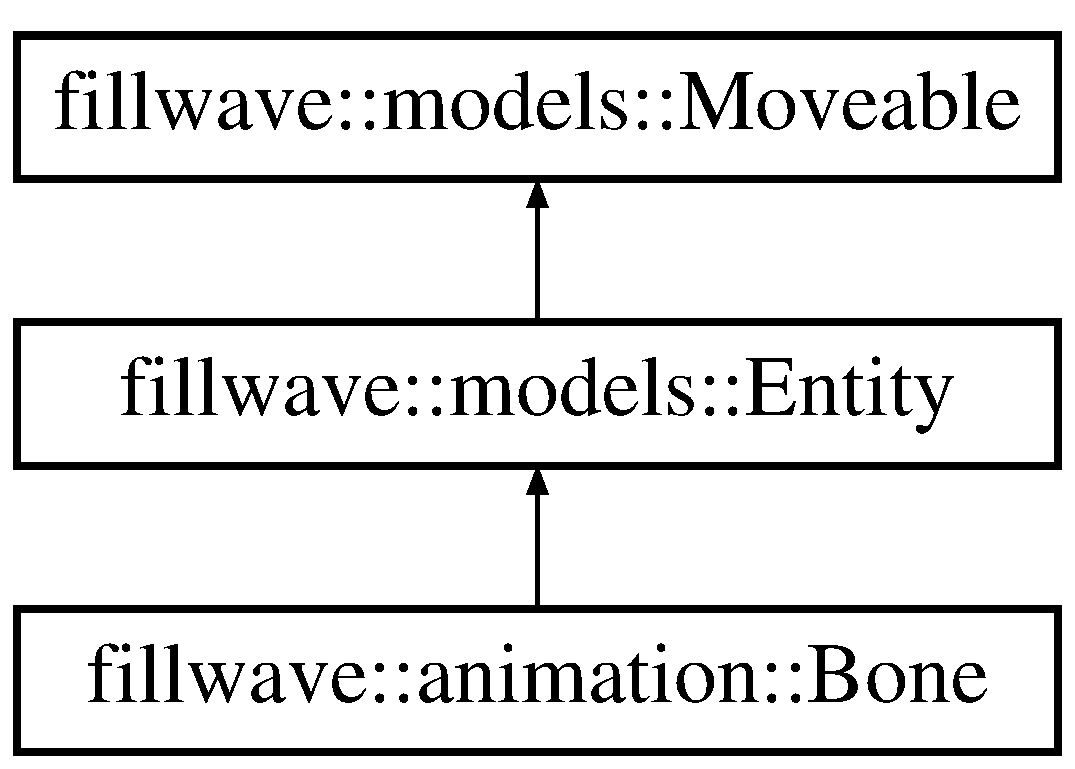
\includegraphics[height=3.000000cm]{classfillwave_1_1animation_1_1Bone}
\end{center}
\end{figure}
\subsection*{Public Member Functions}
\begin{DoxyCompactItemize}
\item 
\hypertarget{classfillwave_1_1animation_1_1Bone_afa7317cf0f1b09facd283417758e56c5}{}{\bfseries Bone} (f\+Bone $\ast$assimp\+Bone)\label{classfillwave_1_1animation_1_1Bone_afa7317cf0f1b09facd283417758e56c5}

\item 
\hypertarget{classfillwave_1_1animation_1_1Bone_aa3ff08b4ea9dca6a1714cc3f0099f97b}{}void {\bfseries set\+Name} (std\+::string name)\label{classfillwave_1_1animation_1_1Bone_aa3ff08b4ea9dca6a1714cc3f0099f97b}

\item 
\hypertarget{classfillwave_1_1animation_1_1Bone_a61463290a15ed77fdee6ae9a252b7352}{}std\+::string {\bfseries get\+Name} ()\label{classfillwave_1_1animation_1_1Bone_a61463290a15ed77fdee6ae9a252b7352}

\item 
\hypertarget{classfillwave_1_1animation_1_1Bone_a425efaefd5f5d05df0dbdffc2fddce04}{}void {\bfseries children\+Update} ()\label{classfillwave_1_1animation_1_1Bone_a425efaefd5f5d05df0dbdffc2fddce04}

\item 
\hypertarget{classfillwave_1_1animation_1_1Bone_a03d9f9b8377b6cde6e8a20babb6ff938}{}glm\+::mat4 {\bfseries get\+Offset\+Matrix} ()\label{classfillwave_1_1animation_1_1Bone_a03d9f9b8377b6cde6e8a20babb6ff938}

\item 
\hypertarget{classfillwave_1_1animation_1_1Bone_a4d2782d1e9bf0f54515d39fd5c025591}{}glm\+::mat4 {\bfseries get\+Global\+Offset\+Matrix} ()\label{classfillwave_1_1animation_1_1Bone_a4d2782d1e9bf0f54515d39fd5c025591}

\item 
\hypertarget{classfillwave_1_1animation_1_1Bone_a2caf977e2956b3a29da98735dc67215a}{}void {\bfseries set\+Offset\+Matrix} (glm\+::mat4 m)\label{classfillwave_1_1animation_1_1Bone_a2caf977e2956b3a29da98735dc67215a}

\item 
\hypertarget{classfillwave_1_1animation_1_1Bone_ac0fb24acdd96adaed1f27312c4ebe98c}{}void {\bfseries set\+Global\+Offset\+Matrix} (glm\+::mat4 m)\label{classfillwave_1_1animation_1_1Bone_ac0fb24acdd96adaed1f27312c4ebe98c}

\item 
\hypertarget{classfillwave_1_1animation_1_1Bone_a57b96cef305fc0b3a93d0dc4fc46f455}{}void {\bfseries log} ()\label{classfillwave_1_1animation_1_1Bone_a57b96cef305fc0b3a93d0dc4fc46f455}

\end{DoxyCompactItemize}
\subsection*{Additional Inherited Members}


\subsection{Detailed Description}
Entity used by Bone\+Manager to perform animation. 

The documentation for this class was generated from the following file\+:\begin{DoxyCompactItemize}
\item 
/home/filip/\+Projects/fillwave/inc/fillwave/animation/Bone.\+h\end{DoxyCompactItemize}

\hypertarget{classfillwave_1_1manager_1_1BoneManager}{}\section{fillwave\+:\+:manager\+:\+:Bone\+Manager Class Reference}
\label{classfillwave_1_1manager_1_1BoneManager}\index{fillwave\+::manager\+::\+Bone\+Manager@{fillwave\+::manager\+::\+Bone\+Manager}}


Manager to handle Bone objects in animation.  




{\ttfamily \#include $<$Bone\+Manager.\+h$>$}

\subsection*{Public Member Functions}
\begin{DoxyCompactItemize}
\item 
\hypertarget{classfillwave_1_1manager_1_1BoneManager_a4fbbe2058b0864ed9e4ad2ba5b5b56a8}{}{\bfseries Bone\+Manager} (const ai\+Scene $\ast$shape)\label{classfillwave_1_1manager_1_1BoneManager_a4fbbe2058b0864ed9e4ad2ba5b5b56a8}

\item 
\hypertarget{classfillwave_1_1manager_1_1BoneManager_a621ed692c7111e2b9dd7c137808f065c}{}void {\bfseries add} (ai\+Bone $\ast$bone)\label{classfillwave_1_1manager_1_1BoneManager_a621ed692c7111e2b9dd7c137808f065c}

\item 
\hypertarget{classfillwave_1_1manager_1_1BoneManager_af6b833b4345494c0b6ca349fa1c9c304}{}void {\bfseries add} (p\+Bone bone)\label{classfillwave_1_1manager_1_1BoneManager_af6b833b4345494c0b6ca349fa1c9c304}

\item 
\hypertarget{classfillwave_1_1manager_1_1BoneManager_a360b85b94d75c652da509e30fd69b3ef}{}void {\bfseries add} (\hyperlink{classfillwave_1_1animation_1_1Animation}{animation\+::\+Animation} $\ast$animation)\label{classfillwave_1_1manager_1_1BoneManager_a360b85b94d75c652da509e30fd69b3ef}

\item 
\hypertarget{classfillwave_1_1manager_1_1BoneManager_a9504984fc6f049e6a58f6aaa7c9ce58a}{}p\+Bone {\bfseries get} (G\+Lint id)\label{classfillwave_1_1manager_1_1BoneManager_a9504984fc6f049e6a58f6aaa7c9ce58a}

\item 
\hypertarget{classfillwave_1_1manager_1_1BoneManager_a7f9edb10a7d59f3053a6bdead8141901}{}p\+Bone {\bfseries get} (std\+::string name)\label{classfillwave_1_1manager_1_1BoneManager_a7f9edb10a7d59f3053a6bdead8141901}

\item 
\hypertarget{classfillwave_1_1manager_1_1BoneManager_a0af9b6724cf868a8883030255e465740}{}G\+Lint {\bfseries get\+Id} (std\+::string name)\label{classfillwave_1_1manager_1_1BoneManager_a0af9b6724cf868a8883030255e465740}

\item 
\hypertarget{classfillwave_1_1manager_1_1BoneManager_afb838c3fa7d4ffe685ccd04811796888}{}G\+Lint {\bfseries get\+Elements} ()\label{classfillwave_1_1manager_1_1BoneManager_afb838c3fa7d4ffe685ccd04811796888}

\item 
\hypertarget{classfillwave_1_1manager_1_1BoneManager_a6b76448aecc4ba7e114e2f2e5ed62812}{}\hyperlink{classfillwave_1_1animation_1_1Animation}{animation\+::\+Animation} $\ast$ {\bfseries get\+Animation} (G\+Lint i)\label{classfillwave_1_1manager_1_1BoneManager_a6b76448aecc4ba7e114e2f2e5ed62812}

\item 
\hypertarget{classfillwave_1_1manager_1_1BoneManager_a47ccfb449d9674c3120ea4d2f0ba62c3}{}G\+Lint {\bfseries get\+Animations} ()\label{classfillwave_1_1manager_1_1BoneManager_a47ccfb449d9674c3120ea4d2f0ba62c3}

\item 
\hypertarget{classfillwave_1_1manager_1_1BoneManager_a911019fc466242c6bf5185910497a47d}{}void {\bfseries log} ()\label{classfillwave_1_1manager_1_1BoneManager_a911019fc466242c6bf5185910497a47d}

\item 
\hypertarget{classfillwave_1_1manager_1_1BoneManager_a83befeb9bce1d44f127cced68a16a45d}{}\hyperlink{classfillwave_1_1animation_1_1Channel}{animation\+::\+Channel} $\ast$ {\bfseries find\+Channel} (\hyperlink{classfillwave_1_1animation_1_1Animation}{animation\+::\+Animation} $\ast$animation, const std\+::string \&node\+Name)\label{classfillwave_1_1manager_1_1BoneManager_a83befeb9bce1d44f127cced68a16a45d}

\item 
\hypertarget{classfillwave_1_1manager_1_1BoneManager_af4c63e5f585324f3804fea03e1adf194}{}glm\+::vec3 {\bfseries get\+Current\+Translation} (float time\+Elapsed\+\_\+s, \hyperlink{classfillwave_1_1animation_1_1Channel}{animation\+::\+Channel} $\ast$channel)\label{classfillwave_1_1manager_1_1BoneManager_af4c63e5f585324f3804fea03e1adf194}

\item 
\hypertarget{classfillwave_1_1manager_1_1BoneManager_ad38cd9c6232b4b1f2ad4c5e59aa9acce}{}glm\+::quat {\bfseries get\+Current\+Rotation} (float time\+Elapsed\+\_\+s, \hyperlink{classfillwave_1_1animation_1_1Channel}{animation\+::\+Channel} $\ast$channel)\label{classfillwave_1_1manager_1_1BoneManager_ad38cd9c6232b4b1f2ad4c5e59aa9acce}

\item 
\hypertarget{classfillwave_1_1manager_1_1BoneManager_a907e6274ff0053ef23a982de3a6c4908}{}glm\+::vec3 {\bfseries get\+Current\+Scale} (float time\+Elapsed\+\_\+s, \hyperlink{classfillwave_1_1animation_1_1Channel}{animation\+::\+Channel} $\ast$channel)\label{classfillwave_1_1manager_1_1BoneManager_a907e6274ff0053ef23a982de3a6c4908}

\item 
\hypertarget{classfillwave_1_1manager_1_1BoneManager_a361968dddf129b4863ce085a9626e69b}{}G\+Luint {\bfseries get\+Translation\+Step} (float time\+Elapsed\+\_\+s, \hyperlink{classfillwave_1_1animation_1_1Channel}{animation\+::\+Channel} $\ast$channel)\label{classfillwave_1_1manager_1_1BoneManager_a361968dddf129b4863ce085a9626e69b}

\item 
\hypertarget{classfillwave_1_1manager_1_1BoneManager_ab508fc08681246625ca9ecc00c9041b1}{}G\+Luint {\bfseries get\+Rotation\+Step} (float time\+Elapsed\+\_\+s, \hyperlink{classfillwave_1_1animation_1_1Channel}{animation\+::\+Channel} $\ast$channel)\label{classfillwave_1_1manager_1_1BoneManager_ab508fc08681246625ca9ecc00c9041b1}

\item 
\hypertarget{classfillwave_1_1manager_1_1BoneManager_a4d4672ca0adb833a6a020cfac655cf62}{}G\+Luint {\bfseries get\+Scale\+Step} (float time\+Elapsed\+\_\+s, \hyperlink{classfillwave_1_1animation_1_1Channel}{animation\+::\+Channel} $\ast$channel)\label{classfillwave_1_1manager_1_1BoneManager_a4d4672ca0adb833a6a020cfac655cf62}

\item 
\hypertarget{classfillwave_1_1manager_1_1BoneManager_ae6e8ddff146f626909b8777c70229d27}{}glm\+::fquat {\bfseries lerp} (const glm\+::fquat \&v0, const glm\+::fquat \&v1, float alpha)\label{classfillwave_1_1manager_1_1BoneManager_ae6e8ddff146f626909b8777c70229d27}

\item 
\hypertarget{classfillwave_1_1manager_1_1BoneManager_a6286be8c76b9244ad1edfd866fb31c5f}{}\hyperlink{classfillwave_1_1manager_1_1AssimpNode}{Assimp\+Node} $\ast$ {\bfseries init\+Node} (ai\+Node $\ast$node)\label{classfillwave_1_1manager_1_1BoneManager_a6286be8c76b9244ad1edfd866fb31c5f}

\item 
\hypertarget{classfillwave_1_1manager_1_1BoneManager_a09eff893aab25b8407251429768363c9}{}void {\bfseries update\+Bones\+Buffer} ()\label{classfillwave_1_1manager_1_1BoneManager_a09eff893aab25b8407251429768363c9}

\item 
\hypertarget{classfillwave_1_1manager_1_1BoneManager_a996a798fc2e1f7e6b6eb18ebfdde6195}{}void {\bfseries update\+Bones\+Uniform} (G\+Lint uniform\+Location\+Bones)\label{classfillwave_1_1manager_1_1BoneManager_a996a798fc2e1f7e6b6eb18ebfdde6195}

\item 
\hypertarget{classfillwave_1_1manager_1_1BoneManager_a55f6856fa921771978b7f8c4001eeba3}{}void {\bfseries update\+Transformations} (G\+Lint active\+Animation, float time\+Elapsed\+\_\+s)\label{classfillwave_1_1manager_1_1BoneManager_a55f6856fa921771978b7f8c4001eeba3}

\end{DoxyCompactItemize}
\subsection*{Public Attributes}
\begin{DoxyCompactItemize}
\item 
\hypertarget{classfillwave_1_1manager_1_1BoneManager_ae65b2366dd24b824412abadde8c80571}{}std\+::vector$<$ \hyperlink{classfillwave_1_1animation_1_1Animation}{animation\+::\+Animation} $\ast$ $>$ {\bfseries m\+Animations}\label{classfillwave_1_1manager_1_1BoneManager_ae65b2366dd24b824412abadde8c80571}

\end{DoxyCompactItemize}


\subsection{Detailed Description}
Manager to handle Bone objects in animation. 

The documentation for this class was generated from the following file\+:\begin{DoxyCompactItemize}
\item 
/home/filip/\+Projects/fillwave/inc/fillwave/management/Bone\+Manager.\+h\end{DoxyCompactItemize}

\hypertarget{classfillwave_1_1effects_1_1BoostColor}{}\section{fillwave\+:\+:effects\+:\+:Boost\+Color Class Reference}
\label{classfillwave_1_1effects_1_1BoostColor}\index{fillwave\+::effects\+::\+Boost\+Color@{fillwave\+::effects\+::\+Boost\+Color}}


\hyperlink{classfillwave_1_1effects_1_1Effect}{Effect} to boost the models color.  




{\ttfamily \#include $<$Boost\+Color.\+h$>$}

Inheritance diagram for fillwave\+:\+:effects\+:\+:Boost\+Color\+:\begin{figure}[H]
\begin{center}
\leavevmode
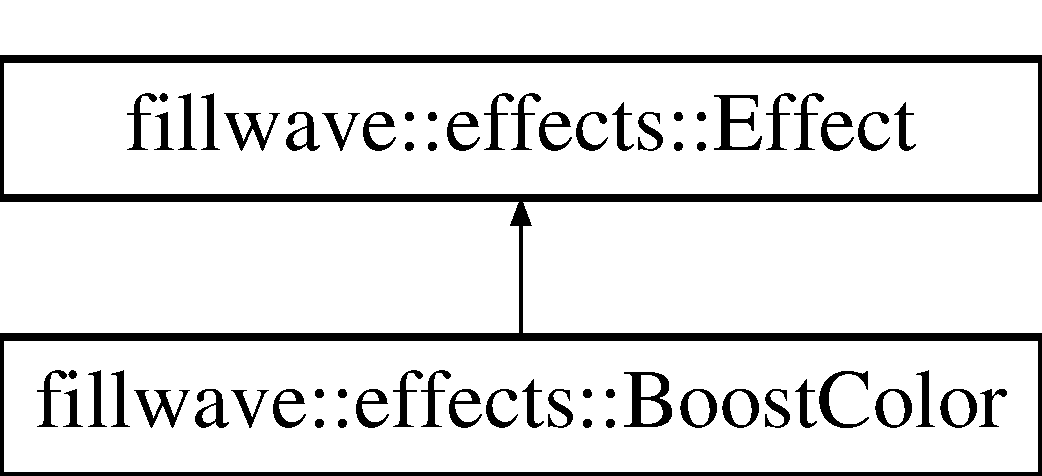
\includegraphics[height=2.000000cm]{classfillwave_1_1effects_1_1BoostColor}
\end{center}
\end{figure}
\subsection*{Public Member Functions}
\begin{DoxyCompactItemize}
\item 
\hypertarget{classfillwave_1_1effects_1_1BoostColor_a6971fc6fc68d3dc3b6aa448164ebb6e2}{}{\bfseries Boost\+Color} (G\+Lfloat boost=1.\+0f)\label{classfillwave_1_1effects_1_1BoostColor_a6971fc6fc68d3dc3b6aa448164ebb6e2}

\item 
void \hyperlink{classfillwave_1_1effects_1_1BoostColor_ae5cbdf0c8487e4ee9743f39f9a6bf247}{pre\+Draw\+Action} (\hyperlink{classfillwave_1_1core_1_1Program}{core\+::\+Program} $\ast$program)
\begin{DoxyCompactList}\small\item\em virtual\+: defines action to be done just before the draw. \end{DoxyCompactList}\item 
void \hyperlink{classfillwave_1_1effects_1_1BoostColor_aeee3b3de532b1ea6aaac80590aa7f081}{post\+Draw\+Action} (\hyperlink{classfillwave_1_1core_1_1Program}{core\+::\+Program} $\ast$program)
\begin{DoxyCompactList}\small\item\em virtual\+: defines action to be done just after the draw. \end{DoxyCompactList}\item 
void \hyperlink{classfillwave_1_1effects_1_1BoostColor_a25ebaad4e773c6a4a147744655955a59}{stop\+Action} (\hyperlink{classfillwave_1_1core_1_1Program}{core\+::\+Program} $\ast$program)
\begin{DoxyCompactList}\small\item\em virtual\+: defines action to be done when the effect is stopped. \end{DoxyCompactList}\item 
void \hyperlink{classfillwave_1_1effects_1_1BoostColor_aad6fdc26934cbdcd0cec735c987e653e}{start\+Action} (\hyperlink{classfillwave_1_1core_1_1Program}{core\+::\+Program} $\ast$program)
\begin{DoxyCompactList}\small\item\em virtual\+: defines action to be done when the effect is started. \end{DoxyCompactList}\end{DoxyCompactItemize}


\subsection{Detailed Description}
\hyperlink{classfillwave_1_1effects_1_1Effect}{Effect} to boost the models color. 

\subsection{Member Function Documentation}
\hypertarget{classfillwave_1_1effects_1_1BoostColor_aeee3b3de532b1ea6aaac80590aa7f081}{}\index{fillwave\+::effects\+::\+Boost\+Color@{fillwave\+::effects\+::\+Boost\+Color}!post\+Draw\+Action@{post\+Draw\+Action}}
\index{post\+Draw\+Action@{post\+Draw\+Action}!fillwave\+::effects\+::\+Boost\+Color@{fillwave\+::effects\+::\+Boost\+Color}}
\subsubsection[{post\+Draw\+Action}]{\setlength{\rightskip}{0pt plus 5cm}void fillwave\+::effects\+::\+Boost\+Color\+::post\+Draw\+Action (
\begin{DoxyParamCaption}
\item[{{\bf core\+::\+Program} $\ast$}]{program}
\end{DoxyParamCaption}
)\hspace{0.3cm}{\ttfamily [virtual]}}\label{classfillwave_1_1effects_1_1BoostColor_aeee3b3de532b1ea6aaac80590aa7f081}


virtual\+: defines action to be done just after the draw. 

post\+Draw\+Action 

Implements \hyperlink{classfillwave_1_1effects_1_1Effect_ae01123633990402e11226c4d9a2dce1b}{fillwave\+::effects\+::\+Effect}.

\hypertarget{classfillwave_1_1effects_1_1BoostColor_ae5cbdf0c8487e4ee9743f39f9a6bf247}{}\index{fillwave\+::effects\+::\+Boost\+Color@{fillwave\+::effects\+::\+Boost\+Color}!pre\+Draw\+Action@{pre\+Draw\+Action}}
\index{pre\+Draw\+Action@{pre\+Draw\+Action}!fillwave\+::effects\+::\+Boost\+Color@{fillwave\+::effects\+::\+Boost\+Color}}
\subsubsection[{pre\+Draw\+Action}]{\setlength{\rightskip}{0pt plus 5cm}void fillwave\+::effects\+::\+Boost\+Color\+::pre\+Draw\+Action (
\begin{DoxyParamCaption}
\item[{{\bf core\+::\+Program} $\ast$}]{program}
\end{DoxyParamCaption}
)\hspace{0.3cm}{\ttfamily [virtual]}}\label{classfillwave_1_1effects_1_1BoostColor_ae5cbdf0c8487e4ee9743f39f9a6bf247}


virtual\+: defines action to be done just before the draw. 

pre\+Draw\+Action 

Implements \hyperlink{classfillwave_1_1effects_1_1Effect_a99c243cb10f504bfc6193e5e81926920}{fillwave\+::effects\+::\+Effect}.

\hypertarget{classfillwave_1_1effects_1_1BoostColor_aad6fdc26934cbdcd0cec735c987e653e}{}\index{fillwave\+::effects\+::\+Boost\+Color@{fillwave\+::effects\+::\+Boost\+Color}!start\+Action@{start\+Action}}
\index{start\+Action@{start\+Action}!fillwave\+::effects\+::\+Boost\+Color@{fillwave\+::effects\+::\+Boost\+Color}}
\subsubsection[{start\+Action}]{\setlength{\rightskip}{0pt plus 5cm}void fillwave\+::effects\+::\+Boost\+Color\+::start\+Action (
\begin{DoxyParamCaption}
\item[{{\bf core\+::\+Program} $\ast$}]{program}
\end{DoxyParamCaption}
)\hspace{0.3cm}{\ttfamily [virtual]}}\label{classfillwave_1_1effects_1_1BoostColor_aad6fdc26934cbdcd0cec735c987e653e}


virtual\+: defines action to be done when the effect is started. 

start\+Action 

Implements \hyperlink{classfillwave_1_1effects_1_1Effect_af0a4aa202fa7201cd19cedf71f6c682a}{fillwave\+::effects\+::\+Effect}.

\hypertarget{classfillwave_1_1effects_1_1BoostColor_a25ebaad4e773c6a4a147744655955a59}{}\index{fillwave\+::effects\+::\+Boost\+Color@{fillwave\+::effects\+::\+Boost\+Color}!stop\+Action@{stop\+Action}}
\index{stop\+Action@{stop\+Action}!fillwave\+::effects\+::\+Boost\+Color@{fillwave\+::effects\+::\+Boost\+Color}}
\subsubsection[{stop\+Action}]{\setlength{\rightskip}{0pt plus 5cm}void fillwave\+::effects\+::\+Boost\+Color\+::stop\+Action (
\begin{DoxyParamCaption}
\item[{{\bf core\+::\+Program} $\ast$}]{program}
\end{DoxyParamCaption}
)\hspace{0.3cm}{\ttfamily [virtual]}}\label{classfillwave_1_1effects_1_1BoostColor_a25ebaad4e773c6a4a147744655955a59}


virtual\+: defines action to be done when the effect is stopped. 

stop\+Action 

Implements \hyperlink{classfillwave_1_1effects_1_1Effect_aed8c053b5798cbbc6668117989d18ead}{fillwave\+::effects\+::\+Effect}.



The documentation for this class was generated from the following file\+:\begin{DoxyCompactItemize}
\item 
/home/filip/\+Projects/fillwave/inc/fillwave/effects/Boost\+Color.\+h\end{DoxyCompactItemize}

\hypertarget{classfillwave_1_1models_1_1Box}{}\section{fillwave\+:\+:models\+:\+:Box Class Reference}
\label{classfillwave_1_1models_1_1Box}\index{fillwave\+::models\+::\+Box@{fillwave\+::models\+::\+Box}}
Inheritance diagram for fillwave\+:\+:models\+:\+:Box\+:\begin{figure}[H]
\begin{center}
\leavevmode
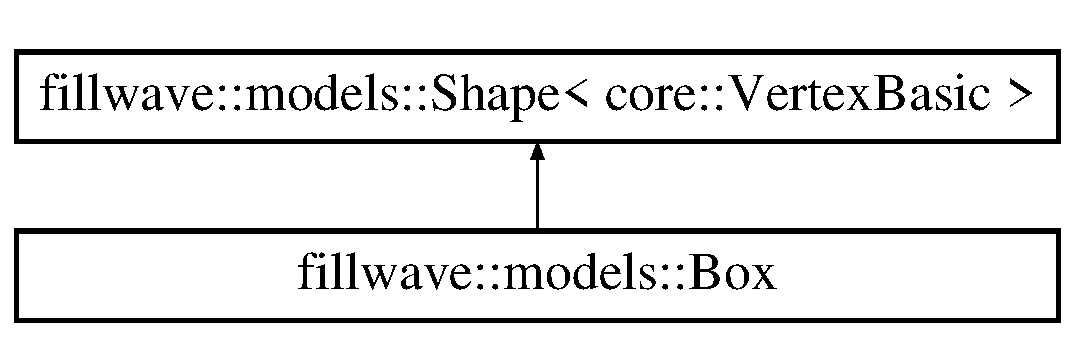
\includegraphics[height=2.000000cm]{classfillwave_1_1models_1_1Box}
\end{center}
\end{figure}
\subsection*{Public Member Functions}
\begin{DoxyCompactItemize}
\item 
\hypertarget{classfillwave_1_1models_1_1Box_ae72150b181cd6030b357c945c6a3307d}{}{\bfseries Box} (G\+Lfloat quad\+Size=1.\+0f)\label{classfillwave_1_1models_1_1Box_ae72150b181cd6030b357c945c6a3307d}

\item 
\hypertarget{classfillwave_1_1models_1_1Box_a5f6af4f2e32428b7974576982aaad817}{}void {\bfseries generate\+Vertices} ()\label{classfillwave_1_1models_1_1Box_a5f6af4f2e32428b7974576982aaad817}

\item 
\hypertarget{classfillwave_1_1models_1_1Box_a5adbb7066f2eb23bbc1f9c8d5d0ac745}{}void {\bfseries generate\+Side} ()\label{classfillwave_1_1models_1_1Box_a5adbb7066f2eb23bbc1f9c8d5d0ac745}

\item 
\hypertarget{classfillwave_1_1models_1_1Box_adbf36225bd9bfa36c9b76f62bbebacf9}{}void {\bfseries generate\+Indices} ()\label{classfillwave_1_1models_1_1Box_adbf36225bd9bfa36c9b76f62bbebacf9}

\end{DoxyCompactItemize}
\subsection*{Additional Inherited Members}


The documentation for this class was generated from the following file\+:\begin{DoxyCompactItemize}
\item 
/home/filip/\+Projects/fillwave/inc/fillwave/models/shapes/Box.\+h\end{DoxyCompactItemize}

\hypertarget{classfillwave_1_1models_1_1BoxOcclusion}{}\section{fillwave\+:\+:models\+:\+:Box\+Occlusion Class Reference}
\label{classfillwave_1_1models_1_1BoxOcclusion}\index{fillwave\+::models\+::\+Box\+Occlusion@{fillwave\+::models\+::\+Box\+Occlusion}}
Inheritance diagram for fillwave\+:\+:models\+:\+:Box\+Occlusion\+:\begin{figure}[H]
\begin{center}
\leavevmode
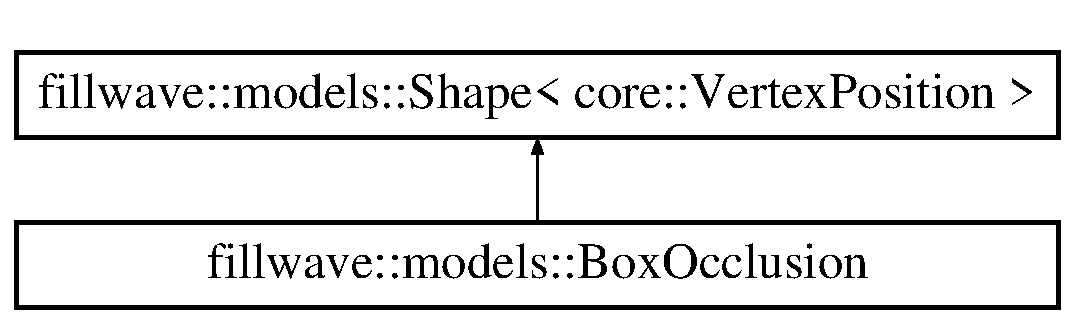
\includegraphics[height=2.000000cm]{classfillwave_1_1models_1_1BoxOcclusion}
\end{center}
\end{figure}
\subsection*{Public Member Functions}
\begin{DoxyCompactItemize}
\item 
\hypertarget{classfillwave_1_1models_1_1BoxOcclusion_a5905ef16915b6a4a8e087b9a68b692e5}{}{\bfseries Box\+Occlusion} (G\+Lfloat quad\+Size=1.\+0f)\label{classfillwave_1_1models_1_1BoxOcclusion_a5905ef16915b6a4a8e087b9a68b692e5}

\end{DoxyCompactItemize}
\subsection*{Additional Inherited Members}


The documentation for this class was generated from the following file\+:\begin{DoxyCompactItemize}
\item 
/home/filip/\+Projects/fillwave/inc/fillwave/models/shapes/Box\+Occlusion.\+h\end{DoxyCompactItemize}

\hypertarget{classfillwave_1_1core_1_1Buffer}{}\section{fillwave\+:\+:core\+:\+:Buffer Class Reference}
\label{classfillwave_1_1core_1_1Buffer}\index{fillwave\+::core\+::\+Buffer@{fillwave\+::core\+::\+Buffer}}


Base for all buffer types.  




{\ttfamily \#include $<$Buffer.\+h$>$}

Inheritance diagram for fillwave\+:\+:core\+:\+:Buffer\+:\begin{figure}[H]
\begin{center}
\leavevmode
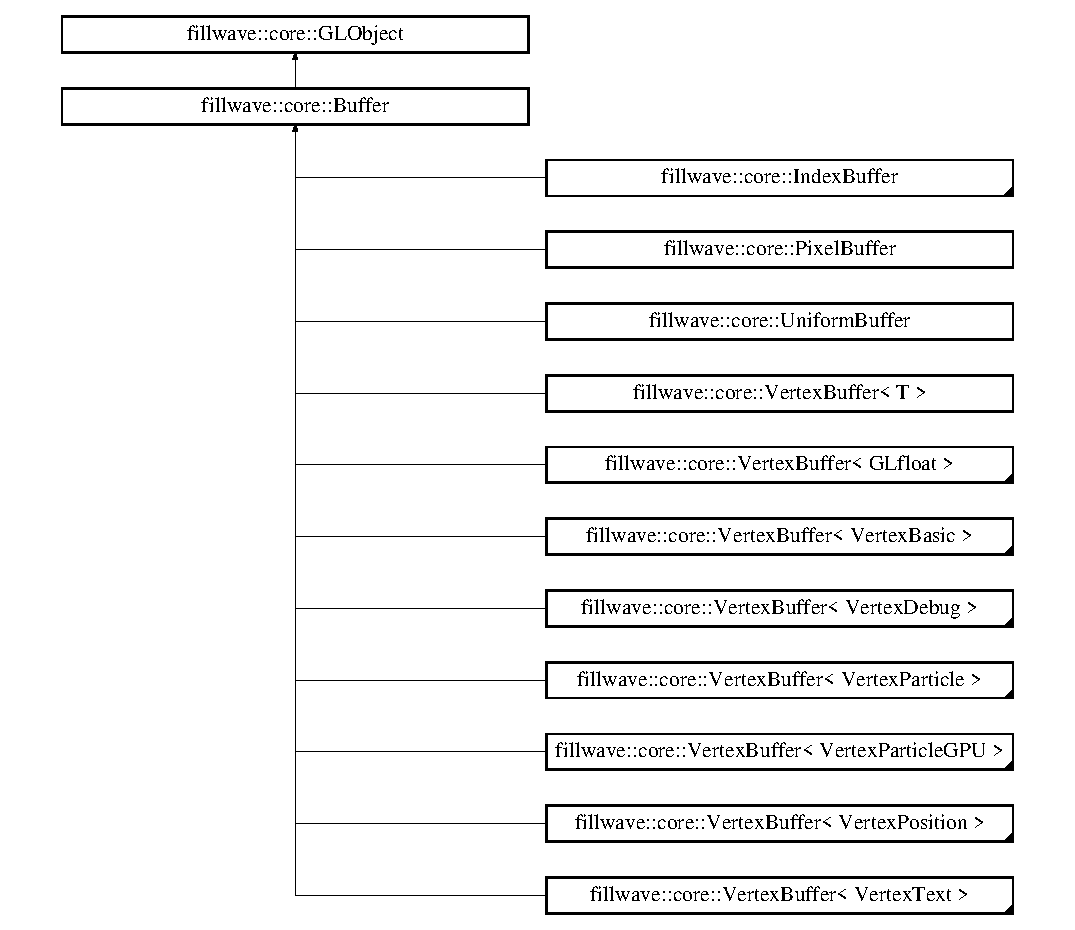
\includegraphics[height=12.000000cm]{classfillwave_1_1core_1_1Buffer}
\end{center}
\end{figure}
\subsection*{Public Member Functions}
\begin{DoxyCompactItemize}
\item 
\hypertarget{classfillwave_1_1core_1_1Buffer_a0eb4bd71707615e42f8b9c5c6b35b4fa}{}{\bfseries Buffer} (G\+Luint target, G\+Luint draw\+Type=G\+L\+\_\+\+S\+T\+A\+T\+I\+C\+\_\+\+D\+R\+A\+W, G\+Luint index=0, G\+Lsizei how\+Many=1)\label{classfillwave_1_1core_1_1Buffer_a0eb4bd71707615e42f8b9c5c6b35b4fa}

\item 
\hypertarget{classfillwave_1_1core_1_1Buffer_a21dfbdb4ff7f15cd6e16ce25c9dc795b}{}void {\bfseries bind} (G\+Luint id=0) const \label{classfillwave_1_1core_1_1Buffer_a21dfbdb4ff7f15cd6e16ce25c9dc795b}

\item 
\hypertarget{classfillwave_1_1core_1_1Buffer_a02eb01c40bcac9358bff281d9d8ef1a0}{}void {\bfseries bind} (G\+Luint external\+Target, G\+Luint id) const \label{classfillwave_1_1core_1_1Buffer_a02eb01c40bcac9358bff281d9d8ef1a0}

\item 
\hypertarget{classfillwave_1_1core_1_1Buffer_a9ae874855b47ce63ee01d033e2c138ed}{}void {\bfseries bind\+Base} (G\+Luint id=0) const \label{classfillwave_1_1core_1_1Buffer_a9ae874855b47ce63ee01d033e2c138ed}

\item 
\hypertarget{classfillwave_1_1core_1_1Buffer_adc36a13505fc5427c69e6d5019fc1eb1}{}void {\bfseries bind\+Base} (G\+Luint external\+Target, G\+Luint id) const \label{classfillwave_1_1core_1_1Buffer_adc36a13505fc5427c69e6d5019fc1eb1}

\item 
\hypertarget{classfillwave_1_1core_1_1Buffer_ac6a6349e4040634ac8f30b63d47267fd}{}void {\bfseries unbind} ()\label{classfillwave_1_1core_1_1Buffer_ac6a6349e4040634ac8f30b63d47267fd}

\item 
\hypertarget{classfillwave_1_1core_1_1Buffer_ab2cc00ce071c66ab404940ed6794e22b}{}void {\bfseries unbind\+Base} (G\+Luint external\+Target)\label{classfillwave_1_1core_1_1Buffer_ab2cc00ce071c66ab404940ed6794e22b}

\item 
\hypertarget{classfillwave_1_1core_1_1Buffer_a8c4dd179a3d765a44368707241d9a5ec}{}G\+Lvoid $\ast$ {\bfseries map\+Range} (G\+Lenum access, G\+Luint size=0)\label{classfillwave_1_1core_1_1Buffer_a8c4dd179a3d765a44368707241d9a5ec}

\item 
\hypertarget{classfillwave_1_1core_1_1Buffer_a35a973f202b6b76d08584811688e15dd}{}void {\bfseries unmap} () const \label{classfillwave_1_1core_1_1Buffer_a35a973f202b6b76d08584811688e15dd}

\item 
\hypertarget{classfillwave_1_1core_1_1Buffer_a27b1cfca70f30c0ba557d236adc4f307}{}void {\bfseries send} ()\label{classfillwave_1_1core_1_1Buffer_a27b1cfca70f30c0ba557d236adc4f307}

\item 
\hypertarget{classfillwave_1_1core_1_1Buffer_a9bc74e68746a7bf35c7265407c6a4ba5}{}void {\bfseries set\+Target} (G\+Luint target)\label{classfillwave_1_1core_1_1Buffer_a9bc74e68746a7bf35c7265407c6a4ba5}

\item 
\hypertarget{classfillwave_1_1core_1_1Buffer_ac39fc2ede4e4c8fa1ac5f65373a4c06f}{}void {\bfseries set\+Draw\+Type} (G\+Luint draw\+Type)\label{classfillwave_1_1core_1_1Buffer_ac39fc2ede4e4c8fa1ac5f65373a4c06f}

\item 
\hypertarget{classfillwave_1_1core_1_1Buffer_aa81fae5c3e9a09708dcd00c4b5166fa0}{}bool {\bfseries is\+Ready} ()\label{classfillwave_1_1core_1_1Buffer_aa81fae5c3e9a09708dcd00c4b5166fa0}

\item 
\hypertarget{classfillwave_1_1core_1_1Buffer_aecad7f7242c6955a78c512830ab2b46d}{}void {\bfseries set\+Ready} ()\label{classfillwave_1_1core_1_1Buffer_aecad7f7242c6955a78c512830ab2b46d}

\item 
\hypertarget{classfillwave_1_1core_1_1Buffer_ab625cd9a2f263af627d20d4f4d73bd5f}{}void {\bfseries reset\+Ready} ()\label{classfillwave_1_1core_1_1Buffer_ab625cd9a2f263af627d20d4f4d73bd5f}

\item 
\hypertarget{classfillwave_1_1core_1_1Buffer_a268b26d5fe54f0372fe07b263320c498}{}G\+Luint {\bfseries get\+Elements} () const \label{classfillwave_1_1core_1_1Buffer_a268b26d5fe54f0372fe07b263320c498}

\item 
\hypertarget{classfillwave_1_1core_1_1Buffer_ad632fd5bb2a53b208a66a32ae449fb0e}{}G\+Luint {\bfseries get\+Size} () const \label{classfillwave_1_1core_1_1Buffer_ad632fd5bb2a53b208a66a32ae449fb0e}

\item 
\hypertarget{classfillwave_1_1core_1_1Buffer_ab4cf69eb6124def11ba0662486735aec}{}G\+Lvoid $\ast$ {\bfseries get\+Data} () const \label{classfillwave_1_1core_1_1Buffer_ab4cf69eb6124def11ba0662486735aec}

\item 
\hypertarget{classfillwave_1_1core_1_1Buffer_afcd11fbdf69f3056ecfcd00cfe2f3966}{}void {\bfseries reload} ()\label{classfillwave_1_1core_1_1Buffer_afcd11fbdf69f3056ecfcd00cfe2f3966}

\item 
\hypertarget{classfillwave_1_1core_1_1Buffer_af4cde11aea152f62a65499d06d66053d}{}G\+Lvoid $\ast$ {\bfseries map} (G\+Lenum access) const \label{classfillwave_1_1core_1_1Buffer_af4cde11aea152f62a65499d06d66053d}

\end{DoxyCompactItemize}
\subsection*{Protected Member Functions}
\begin{DoxyCompactItemize}
\item 
\hypertarget{classfillwave_1_1core_1_1Buffer_a470d1b51f2b2d2d6d8a5dce29358c1f9}{}void {\bfseries set\+Elements} (G\+Luint elements)\label{classfillwave_1_1core_1_1Buffer_a470d1b51f2b2d2d6d8a5dce29358c1f9}

\item 
\hypertarget{classfillwave_1_1core_1_1Buffer_a890a440f8ea28e984a9bdfa7949ef427}{}void {\bfseries set\+Size} (G\+Luint size)\label{classfillwave_1_1core_1_1Buffer_a890a440f8ea28e984a9bdfa7949ef427}

\end{DoxyCompactItemize}
\subsection*{Protected Attributes}
\begin{DoxyCompactItemize}
\item 
\hypertarget{classfillwave_1_1core_1_1Buffer_a32235dd78b278c04bd98035ed8375d19}{}G\+Luint {\bfseries m\+Index}\label{classfillwave_1_1core_1_1Buffer_a32235dd78b278c04bd98035ed8375d19}

\item 
\hypertarget{classfillwave_1_1core_1_1Buffer_a2559c70d5a09568a50d3091e69d45bb1}{}G\+Luint {\bfseries m\+Target}\label{classfillwave_1_1core_1_1Buffer_a2559c70d5a09568a50d3091e69d45bb1}

\item 
\hypertarget{classfillwave_1_1core_1_1Buffer_ab2b3a6934a4adb261723f1ff45b815d1}{}G\+Luint {\bfseries m\+Data\+Store\+Type}\label{classfillwave_1_1core_1_1Buffer_ab2b3a6934a4adb261723f1ff45b815d1}

\item 
\hypertarget{classfillwave_1_1core_1_1Buffer_ae4dc20c18344d5a3ce899ae598978d8c}{}G\+Lboolean {\bfseries m\+Refresh}\label{classfillwave_1_1core_1_1Buffer_ae4dc20c18344d5a3ce899ae598978d8c}

\item 
\hypertarget{classfillwave_1_1core_1_1Buffer_af86f454d76ba53946831c3fe9aadb51c}{}G\+Lvoid $\ast$ {\bfseries m\+Data}\label{classfillwave_1_1core_1_1Buffer_af86f454d76ba53946831c3fe9aadb51c}

\item 
\hypertarget{classfillwave_1_1core_1_1Buffer_ab4062f2530e6cedfd4bac04405d7bf8b}{}G\+Luint {\bfseries m\+Size}\label{classfillwave_1_1core_1_1Buffer_ab4062f2530e6cedfd4bac04405d7bf8b}

\item 
\hypertarget{classfillwave_1_1core_1_1Buffer_aaf51ae619c24a67411c7cd08aa6d3d92}{}G\+Luint {\bfseries m\+Total\+Elements}\label{classfillwave_1_1core_1_1Buffer_aaf51ae619c24a67411c7cd08aa6d3d92}

\end{DoxyCompactItemize}


\subsection{Detailed Description}
Base for all buffer types. 

The documentation for this class was generated from the following file\+:\begin{DoxyCompactItemize}
\item 
/home/filip/\+Projects/fillwave/inc/fillwave/core/buffers/Buffer.\+h\end{DoxyCompactItemize}

\hypertarget{classfillwave_1_1manager_1_1BufferManager}{}\section{fillwave\+:\+:manager\+:\+:Buffer\+Manager Class Reference}
\label{classfillwave_1_1manager_1_1BufferManager}\index{fillwave\+::manager\+::\+Buffer\+Manager@{fillwave\+::manager\+::\+Buffer\+Manager}}


Not used.  




{\ttfamily \#include $<$Buffer\+Manager.\+h$>$}

\subsection*{Public Member Functions}
\begin{DoxyCompactItemize}
\item 
\hypertarget{classfillwave_1_1manager_1_1BufferManager_a8be66b70766ca69dd3e28d658a71dc9e}{}void {\bfseries collect\+Garbage} ()\label{classfillwave_1_1manager_1_1BufferManager_a8be66b70766ca69dd3e28d658a71dc9e}

\item 
\hypertarget{classfillwave_1_1manager_1_1BufferManager_ab47918353827a659c6edb89a5ab0ba28}{}void {\bfseries reload} ()\label{classfillwave_1_1manager_1_1BufferManager_ab47918353827a659c6edb89a5ab0ba28}

\item 
\hypertarget{classfillwave_1_1manager_1_1BufferManager_a6f43be3ce2b753eb9f4b52e2947745dd}{}p\+Vertex\+Array {\bfseries get\+V\+A\+O} (\hyperlink{classfillwave_1_1models_1_1Reloadable}{models\+::\+Reloadable} $\ast$renderable)\label{classfillwave_1_1manager_1_1BufferManager_a6f43be3ce2b753eb9f4b52e2947745dd}

\end{DoxyCompactItemize}


\subsection{Detailed Description}
Not used. 

The documentation for this class was generated from the following file\+:\begin{DoxyCompactItemize}
\item 
/home/filip/\+Projects/fillwave/inc/fillwave/management/Buffer\+Manager.\+h\end{DoxyCompactItemize}

\hypertarget{classfillwave_1_1particles_1_1BuilderEmiter}{}\section{fillwave\+:\+:particles\+:\+:Builder\+Emiter Class Reference}
\label{classfillwave_1_1particles_1_1BuilderEmiter}\index{fillwave\+::particles\+::\+Builder\+Emiter@{fillwave\+::particles\+::\+Builder\+Emiter}}


Builder\+Model which builds the particles emiter.  




{\ttfamily \#include $<$Builder\+Emiter.\+h$>$}

\subsection*{Public Member Functions}
\begin{DoxyCompactItemize}
\item 
\hypertarget{classfillwave_1_1particles_1_1BuilderEmiter_aead03a2d1cb28baf37352474d8af07e5}{}{\bfseries Builder\+Emiter} (\hyperlink{classfillwave_1_1Engine}{Engine} $\ast$engine)\label{classfillwave_1_1particles_1_1BuilderEmiter_aead03a2d1cb28baf37352474d8af07e5}

\item 
\hypertarget{classfillwave_1_1particles_1_1BuilderEmiter_a76d8c1a9d22169c6d5eacad94c791d66}{}\hyperlink{classfillwave_1_1particles_1_1BuilderEmiter}{Builder\+Emiter} \& {\bfseries set\+Emiting\+Source\+Rate} (G\+Lfloat emiting\+Source\+Rate)\label{classfillwave_1_1particles_1_1BuilderEmiter_a76d8c1a9d22169c6d5eacad94c791d66}

\item 
\hypertarget{classfillwave_1_1particles_1_1BuilderEmiter_a06924d9a033c92dc5d2e8a357fcd78d3}{}\hyperlink{classfillwave_1_1particles_1_1BuilderEmiter}{Builder\+Emiter} \& {\bfseries set\+How\+Many} (G\+Luint howmany)\label{classfillwave_1_1particles_1_1BuilderEmiter_a06924d9a033c92dc5d2e8a357fcd78d3}

\item 
\hypertarget{classfillwave_1_1particles_1_1BuilderEmiter_aa011bf626ba6a54421aaef1dcab1a7b1}{}\hyperlink{classfillwave_1_1particles_1_1BuilderEmiter}{Builder\+Emiter} \& {\bfseries set\+Color} (glm\+::vec4 color)\label{classfillwave_1_1particles_1_1BuilderEmiter_aa011bf626ba6a54421aaef1dcab1a7b1}

\item 
\hypertarget{classfillwave_1_1particles_1_1BuilderEmiter_a8049f7650b71e737c5d51779f9804425}{}\hyperlink{classfillwave_1_1particles_1_1BuilderEmiter}{Builder\+Emiter} \& {\bfseries set\+Acceleration} (glm\+::vec3 acceleration)\label{classfillwave_1_1particles_1_1BuilderEmiter_a8049f7650b71e737c5d51779f9804425}

\item 
\hypertarget{classfillwave_1_1particles_1_1BuilderEmiter_aecde24c4ef87af4bd5c20b45e15b0099}{}\hyperlink{classfillwave_1_1particles_1_1BuilderEmiter}{Builder\+Emiter} \& {\bfseries set\+Start\+Velocity} (glm\+::vec3 start\+Velocity)\label{classfillwave_1_1particles_1_1BuilderEmiter_aecde24c4ef87af4bd5c20b45e15b0099}

\item 
\hypertarget{classfillwave_1_1particles_1_1BuilderEmiter_aaecd2082d38b26b48345b830c65fd7ea}{}\hyperlink{classfillwave_1_1particles_1_1BuilderEmiter}{Builder\+Emiter} \& {\bfseries set\+Robustness\+Velocity} (glm\+::vec3 robustness\+Velocity)\label{classfillwave_1_1particles_1_1BuilderEmiter_aaecd2082d38b26b48345b830c65fd7ea}

\item 
\hypertarget{classfillwave_1_1particles_1_1BuilderEmiter_a4665d7c6d1d006a49b0d7ec8a5114b0c}{}\hyperlink{classfillwave_1_1particles_1_1BuilderEmiter}{Builder\+Emiter} \& {\bfseries set\+Start\+Position} (glm\+::vec3 start\+Position)\label{classfillwave_1_1particles_1_1BuilderEmiter_a4665d7c6d1d006a49b0d7ec8a5114b0c}

\item 
\hypertarget{classfillwave_1_1particles_1_1BuilderEmiter_a4291a20dd0753ed1bb62395049890b30}{}\hyperlink{classfillwave_1_1particles_1_1BuilderEmiter}{Builder\+Emiter} \& {\bfseries set\+Robustness\+Position} (glm\+::vec3 robustness\+Position)\label{classfillwave_1_1particles_1_1BuilderEmiter_a4291a20dd0753ed1bb62395049890b30}

\item 
\hypertarget{classfillwave_1_1particles_1_1BuilderEmiter_a4ad8fb8f56465993fff9ccee81c214a1}{}\hyperlink{classfillwave_1_1particles_1_1BuilderEmiter}{Builder\+Emiter} \& {\bfseries set\+Start\+Size} (G\+Lfloat size)\label{classfillwave_1_1particles_1_1BuilderEmiter_a4ad8fb8f56465993fff9ccee81c214a1}

\item 
\hypertarget{classfillwave_1_1particles_1_1BuilderEmiter_afc9f9966ee305ff9fb726431209cc016}{}\hyperlink{classfillwave_1_1particles_1_1BuilderEmiter}{Builder\+Emiter} \& {\bfseries set\+Lifetime} (G\+Lfloat lifetime)\label{classfillwave_1_1particles_1_1BuilderEmiter_afc9f9966ee305ff9fb726431209cc016}

\item 
\hypertarget{classfillwave_1_1particles_1_1BuilderEmiter_a843140630a1f727b1211554dbac3f1a8}{}\hyperlink{classfillwave_1_1particles_1_1BuilderEmiter}{Builder\+Emiter} \& {\bfseries set\+Texture} (p\+Texture texture)\label{classfillwave_1_1particles_1_1BuilderEmiter_a843140630a1f727b1211554dbac3f1a8}

\item 
\hypertarget{classfillwave_1_1particles_1_1BuilderEmiter_a1d2f912255203773f1e7d7cad0a005be}{}\hyperlink{classfillwave_1_1particles_1_1BuilderEmiter}{Builder\+Emiter} \& {\bfseries set\+Blending\+Source} (G\+Lenum source\+Color)\label{classfillwave_1_1particles_1_1BuilderEmiter_a1d2f912255203773f1e7d7cad0a005be}

\item 
\hypertarget{classfillwave_1_1particles_1_1BuilderEmiter_af95ac02fc0ca1028c2d24645d6ce375b}{}\hyperlink{classfillwave_1_1particles_1_1BuilderEmiter}{Builder\+Emiter} \& {\bfseries set\+Blending\+Destination} (G\+Lenum destination\+Color)\label{classfillwave_1_1particles_1_1BuilderEmiter_af95ac02fc0ca1028c2d24645d6ce375b}

\item 
\hypertarget{classfillwave_1_1particles_1_1BuilderEmiter_a95a6d92e796c5c1e7f4bd0cd818dac95}{}\hyperlink{classfillwave_1_1particles_1_1BuilderEmiter}{Builder\+Emiter} \& {\bfseries set\+Depth\+Testing} (G\+Lboolean depth\+Testing)\label{classfillwave_1_1particles_1_1BuilderEmiter_a95a6d92e796c5c1e7f4bd0cd818dac95}

\item 
\hypertarget{classfillwave_1_1particles_1_1BuilderEmiter_a0d53a8cdc2f8f5a3309bc4164f045db4}{}\hyperlink{classfillwave_1_1particles_1_1BuilderEmiter}{Builder\+Emiter} \& {\bfseries set\+Alpha\+Cut\+Off} (G\+Lfloat cut\+Off\+Level)\label{classfillwave_1_1particles_1_1BuilderEmiter_a0d53a8cdc2f8f5a3309bc4164f045db4}

\item 
\hypertarget{classfillwave_1_1particles_1_1BuilderEmiter_a7db80688312b1ee3d369192ef15f868a}{}p\+Emiter\+Point {\bfseries build\+Emiter\+G\+P\+U} ()\label{classfillwave_1_1particles_1_1BuilderEmiter_a7db80688312b1ee3d369192ef15f868a}

\item 
\hypertarget{classfillwave_1_1particles_1_1BuilderEmiter_a288fcdf3212a2621112c011ddd63ccc2}{}p\+Emiter\+Point {\bfseries build\+Emiter\+C\+P\+U} ()\label{classfillwave_1_1particles_1_1BuilderEmiter_a288fcdf3212a2621112c011ddd63ccc2}

\end{DoxyCompactItemize}


\subsection{Detailed Description}
Builder\+Model which builds the particles emiter. 

The documentation for this class was generated from the following file\+:\begin{DoxyCompactItemize}
\item 
/home/filip/\+Projects/fillwave/inc/fillwave/particles/Builder\+Emiter.\+h\end{DoxyCompactItemize}

\hypertarget{classfillwave_1_1models_1_1BuilderModel}{}\section{fillwave\+:\+:models\+:\+:Builder\+Model Class Reference}
\label{classfillwave_1_1models_1_1BuilderModel}\index{fillwave\+::models\+::\+Builder\+Model@{fillwave\+::models\+::\+Builder\+Model}}


Builder which builds the model from the asset file.  




{\ttfamily \#include $<$Builder\+Model.\+h$>$}

Inheritance diagram for fillwave\+:\+:models\+:\+:Builder\+Model\+:\begin{figure}[H]
\begin{center}
\leavevmode
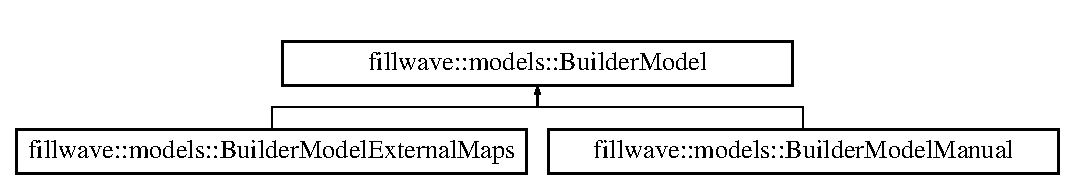
\includegraphics[height=2.000000cm]{classfillwave_1_1models_1_1BuilderModel}
\end{center}
\end{figure}
\subsection*{Public Member Functions}
\begin{DoxyCompactItemize}
\item 
\hypertarget{classfillwave_1_1models_1_1BuilderModel_ae7ed2ae0486af650bad110f7f9d41b3e}{}{\bfseries Builder\+Model} (\hyperlink{classfillwave_1_1Engine}{Engine} $\ast$engine, std\+::string model\+Path, p\+Program program)\label{classfillwave_1_1models_1_1BuilderModel_ae7ed2ae0486af650bad110f7f9d41b3e}

\item 
\hypertarget{classfillwave_1_1models_1_1BuilderModel_ae1dfaa700dda4f97021a543139194408}{}virtual p\+Model {\bfseries build} ()\label{classfillwave_1_1models_1_1BuilderModel_ae1dfaa700dda4f97021a543139194408}

\item 
\hypertarget{classfillwave_1_1models_1_1BuilderModel_a6f79f1bfa7fa74173e0414562fe9459e}{}\hyperlink{classfillwave_1_1models_1_1BuilderModel}{Builder\+Model} \& {\bfseries set\+Model\+Path} (std\+::string \&path)\label{classfillwave_1_1models_1_1BuilderModel_a6f79f1bfa7fa74173e0414562fe9459e}

\item 
\hypertarget{classfillwave_1_1models_1_1BuilderModel_ae6f0837d2abfdc3de31fcc774104396b}{}\hyperlink{classfillwave_1_1models_1_1BuilderModel}{Builder\+Model} \& {\bfseries set\+Program} (p\+Program program)\label{classfillwave_1_1models_1_1BuilderModel_ae6f0837d2abfdc3de31fcc774104396b}

\end{DoxyCompactItemize}
\subsection*{Protected Attributes}
\begin{DoxyCompactItemize}
\item 
\hypertarget{classfillwave_1_1models_1_1BuilderModel_a28590661c540b4afa0effaa027a93931}{}\hyperlink{classfillwave_1_1Engine}{Engine} $\ast$ {\bfseries m\+Engine}\label{classfillwave_1_1models_1_1BuilderModel_a28590661c540b4afa0effaa027a93931}

\item 
\hypertarget{classfillwave_1_1models_1_1BuilderModel_aca82bb8958792ebe5cfe73971e10ba4f}{}p\+Program {\bfseries m\+Program}\label{classfillwave_1_1models_1_1BuilderModel_aca82bb8958792ebe5cfe73971e10ba4f}

\item 
\hypertarget{classfillwave_1_1models_1_1BuilderModel_a7b39d4d8e21413b1f01cf637349f5f57}{}std\+::string {\bfseries m\+Shape\+Path}\label{classfillwave_1_1models_1_1BuilderModel_a7b39d4d8e21413b1f01cf637349f5f57}

\end{DoxyCompactItemize}


\subsection{Detailed Description}
Builder which builds the model from the asset file. 

The documentation for this class was generated from the following file\+:\begin{DoxyCompactItemize}
\item 
/home/filip/\+Projects/fillwave/inc/fillwave/models/Builder\+Model.\+h\end{DoxyCompactItemize}

\hypertarget{classfillwave_1_1models_1_1BuilderModelExternalMaps}{}\section{fillwave\+:\+:models\+:\+:Builder\+Model\+External\+Maps Class Reference}
\label{classfillwave_1_1models_1_1BuilderModelExternalMaps}\index{fillwave\+::models\+::\+Builder\+Model\+External\+Maps@{fillwave\+::models\+::\+Builder\+Model\+External\+Maps}}


\hyperlink{classfillwave_1_1models_1_1BuilderModel}{Builder\+Model} which builds the model from the asset file but uses external texture maps.  




{\ttfamily \#include $<$Builder\+Model\+External\+Maps.\+h$>$}

Inheritance diagram for fillwave\+:\+:models\+:\+:Builder\+Model\+External\+Maps\+:\begin{figure}[H]
\begin{center}
\leavevmode
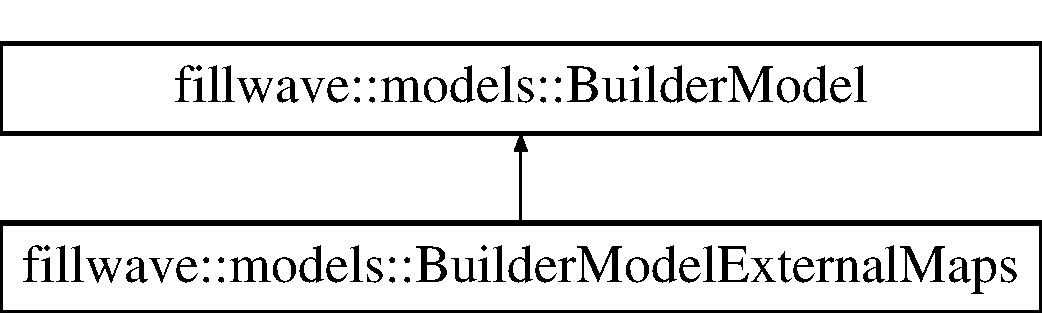
\includegraphics[height=2.000000cm]{classfillwave_1_1models_1_1BuilderModelExternalMaps}
\end{center}
\end{figure}
\subsection*{Public Member Functions}
\begin{DoxyCompactItemize}
\item 
\hypertarget{classfillwave_1_1models_1_1BuilderModelExternalMaps_ab57ba7e42d5ad724114f26e81c313b5d}{}{\bfseries Builder\+Model\+External\+Maps} (\hyperlink{classfillwave_1_1Engine}{Engine} $\ast$engine, std\+::string model\+Path=\char`\"{}\char`\"{}, p\+Program program=p\+Program(), std\+::string diffuse\+Path=\char`\"{}\char`\"{}, std\+::string normal\+Path=\char`\"{}\char`\"{}, std\+::string specular\+Path=\char`\"{}\char`\"{})\label{classfillwave_1_1models_1_1BuilderModelExternalMaps_ab57ba7e42d5ad724114f26e81c313b5d}

\item 
\hypertarget{classfillwave_1_1models_1_1BuilderModelExternalMaps_a8456aeade192f50ed4d8ea369c90f237}{}\hyperlink{classfillwave_1_1models_1_1BuilderModel}{Builder\+Model} \& {\bfseries setdiffuse\+Path} (std\+::string \&path)\label{classfillwave_1_1models_1_1BuilderModelExternalMaps_a8456aeade192f50ed4d8ea369c90f237}

\item 
\hypertarget{classfillwave_1_1models_1_1BuilderModelExternalMaps_a35b04004cdf43446f0ababa8d1f57ccf}{}\hyperlink{classfillwave_1_1models_1_1BuilderModel}{Builder\+Model} \& {\bfseries set\+Normal\+Map\+Path} (std\+::string \&path)\label{classfillwave_1_1models_1_1BuilderModelExternalMaps_a35b04004cdf43446f0ababa8d1f57ccf}

\item 
\hypertarget{classfillwave_1_1models_1_1BuilderModelExternalMaps_a30ef4ffc1a4d9395a25e34bb60a8c4aa}{}\hyperlink{classfillwave_1_1models_1_1BuilderModel}{Builder\+Model} \& {\bfseries set\+Specular\+Map\+Path} (std\+::string \&path)\label{classfillwave_1_1models_1_1BuilderModelExternalMaps_a30ef4ffc1a4d9395a25e34bb60a8c4aa}

\item 
\hypertarget{classfillwave_1_1models_1_1BuilderModelExternalMaps_aaedc7219663a04ac39b46ac670204b86}{}p\+Model {\bfseries build} ()\label{classfillwave_1_1models_1_1BuilderModelExternalMaps_aaedc7219663a04ac39b46ac670204b86}

\end{DoxyCompactItemize}
\subsection*{Additional Inherited Members}


\subsection{Detailed Description}
\hyperlink{classfillwave_1_1models_1_1BuilderModel}{Builder\+Model} which builds the model from the asset file but uses external texture maps. 

The documentation for this class was generated from the following file\+:\begin{DoxyCompactItemize}
\item 
/home/filip/\+Projects/fillwave/inc/fillwave/models/Builder\+Model\+External\+Maps.\+h\end{DoxyCompactItemize}

\hypertarget{classfillwave_1_1models_1_1BuilderModelManual}{}\section{fillwave\+:\+:models\+:\+:Builder\+Model\+Manual Class Reference}
\label{classfillwave_1_1models_1_1BuilderModelManual}\index{fillwave\+::models\+::\+Builder\+Model\+Manual@{fillwave\+::models\+::\+Builder\+Model\+Manual}}


\hyperlink{classfillwave_1_1models_1_1BuilderModel}{Builder\+Model} which builds the model from textures and material fillwave objects.  




{\ttfamily \#include $<$Builder\+Model\+Manual.\+h$>$}

Inheritance diagram for fillwave\+:\+:models\+:\+:Builder\+Model\+Manual\+:\begin{figure}[H]
\begin{center}
\leavevmode
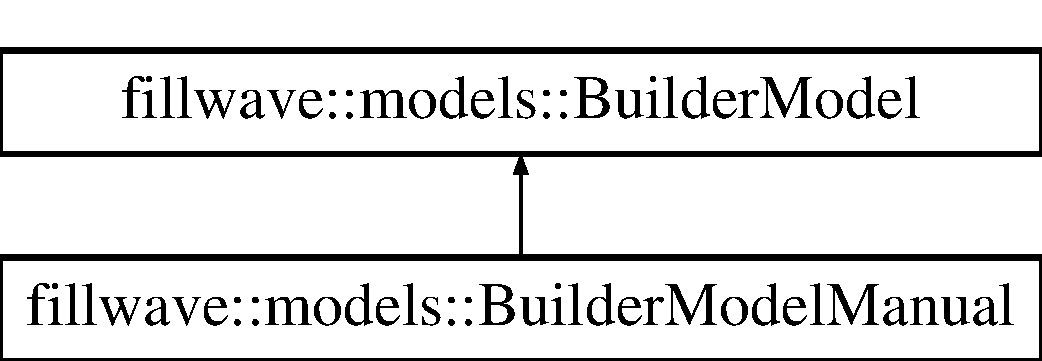
\includegraphics[height=2.000000cm]{classfillwave_1_1models_1_1BuilderModelManual}
\end{center}
\end{figure}
\subsection*{Public Member Functions}
\begin{DoxyCompactItemize}
\item 
\hypertarget{classfillwave_1_1models_1_1BuilderModelManual_ae16bb5619140123b1446ea6742a3a17b}{}{\bfseries Builder\+Model\+Manual} (\hyperlink{classfillwave_1_1Engine}{Engine} $\ast$engine, std\+::string model\+Path=\char`\"{}\char`\"{}, p\+Program program=p\+Program(), p\+Texture diffuse\+Map=p\+Texture(), p\+Texture normal\+Map=p\+Texture(), p\+Texture specular\+Map=p\+Texture(), \hyperlink{classfillwave_1_1models_1_1Material}{Material} material=\hyperlink{classfillwave_1_1models_1_1Material}{Material}())\label{classfillwave_1_1models_1_1BuilderModelManual_ae16bb5619140123b1446ea6742a3a17b}

\item 
\hypertarget{classfillwave_1_1models_1_1BuilderModelManual_ace188d0d7cf3af006137b930fc44a0d0}{}\hyperlink{classfillwave_1_1models_1_1BuilderModelManual}{Builder\+Model\+Manual} \& {\bfseries set\+Diffuse\+Map\+Texture} (p\+Texture texture)\label{classfillwave_1_1models_1_1BuilderModelManual_ace188d0d7cf3af006137b930fc44a0d0}

\item 
\hypertarget{classfillwave_1_1models_1_1BuilderModelManual_af386bc9269b82922dc99f847ef85e226}{}\hyperlink{classfillwave_1_1models_1_1BuilderModelManual}{Builder\+Model\+Manual} \& {\bfseries set\+Normal\+Map\+Texture} (p\+Texture texture)\label{classfillwave_1_1models_1_1BuilderModelManual_af386bc9269b82922dc99f847ef85e226}

\item 
\hypertarget{classfillwave_1_1models_1_1BuilderModelManual_a4940ba4e2067c4b7b403825aad4ebaff}{}\hyperlink{classfillwave_1_1models_1_1BuilderModelManual}{Builder\+Model\+Manual} \& {\bfseries set\+Specular\+Map\+Texture} (p\+Texture texture)\label{classfillwave_1_1models_1_1BuilderModelManual_a4940ba4e2067c4b7b403825aad4ebaff}

\item 
\hypertarget{classfillwave_1_1models_1_1BuilderModelManual_ab59b00511f4cc4c08fa34589fcb88918}{}\hyperlink{classfillwave_1_1models_1_1BuilderModelManual}{Builder\+Model\+Manual} \& {\bfseries set\+Material} (\hyperlink{classfillwave_1_1models_1_1Material}{Material} material)\label{classfillwave_1_1models_1_1BuilderModelManual_ab59b00511f4cc4c08fa34589fcb88918}

\item 
\hypertarget{classfillwave_1_1models_1_1BuilderModelManual_a8ec62dc9a91ed585dd9d3830069897b7}{}p\+Model {\bfseries build} ()\label{classfillwave_1_1models_1_1BuilderModelManual_a8ec62dc9a91ed585dd9d3830069897b7}

\end{DoxyCompactItemize}
\subsection*{Additional Inherited Members}


\subsection{Detailed Description}
\hyperlink{classfillwave_1_1models_1_1BuilderModel}{Builder\+Model} which builds the model from textures and material fillwave objects. 

The documentation for this class was generated from the following file\+:\begin{DoxyCompactItemize}
\item 
/home/filip/\+Projects/fillwave/inc/fillwave/models/Builder\+Model\+Manual.\+h\end{DoxyCompactItemize}

\hypertarget{classfillwave_1_1actions_1_1Callback}{}\section{fillwave\+:\+:actions\+:\+:Callback Class Reference}
\label{classfillwave_1_1actions_1_1Callback}\index{fillwave\+::actions\+::\+Callback@{fillwave\+::actions\+::\+Callback}}


Base for all callbacks.  




{\ttfamily \#include $<$Callback.\+h$>$}

Inheritance diagram for fillwave\+:\+:actions\+:\+:Callback\+:\begin{figure}[H]
\begin{center}
\leavevmode
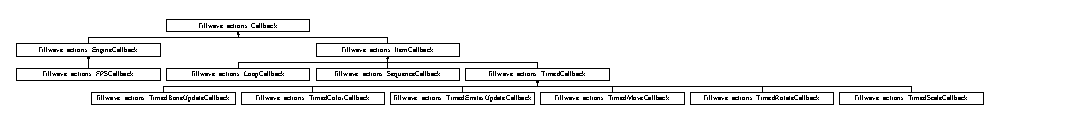
\includegraphics[height=1.180812cm]{classfillwave_1_1actions_1_1Callback}
\end{center}
\end{figure}
\subsection*{Public Member Functions}
\begin{DoxyCompactItemize}
\item 
\hypertarget{classfillwave_1_1actions_1_1Callback_a335073b7711a88b49b6843c6141784c2}{}{\bfseries Callback} (e\+Event\+Type event\+Type)\label{classfillwave_1_1actions_1_1Callback_a335073b7711a88b49b6843c6141784c2}

\item 
\hypertarget{classfillwave_1_1actions_1_1Callback_acc454aa8b6d8f16c40979adecc5f4d14}{}e\+Event\+Type {\bfseries get\+Supported\+Event\+Type} ()\label{classfillwave_1_1actions_1_1Callback_acc454aa8b6d8f16c40979adecc5f4d14}

\end{DoxyCompactItemize}


\subsection{Detailed Description}
Base for all callbacks. 

The documentation for this class was generated from the following file\+:\begin{DoxyCompactItemize}
\item 
/home/filip/\+Projects/fillwave/inc/fillwave/actions/Callback.\+h\end{DoxyCompactItemize}

\hypertarget{classfillwave_1_1space_1_1Camera}{}\section{fillwave\+:\+:space\+:\+:Camera Class Reference}
\label{classfillwave_1_1space_1_1Camera}\index{fillwave\+::space\+::\+Camera@{fillwave\+::space\+::\+Camera}}


Stores camera view parameters.  




{\ttfamily \#include $<$Camera.\+h$>$}

Inheritance diagram for fillwave\+:\+:space\+:\+:Camera\+:\begin{figure}[H]
\begin{center}
\leavevmode
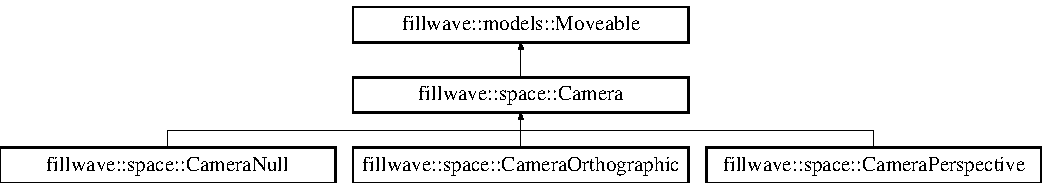
\includegraphics[height=1.842105cm]{classfillwave_1_1space_1_1Camera}
\end{center}
\end{figure}
\subsection*{Public Member Functions}
\begin{DoxyCompactItemize}
\item 
\hypertarget{classfillwave_1_1space_1_1Camera_a489acd9c53c9bf0ab1311f2f2bcbd9c2}{}{\bfseries Camera} (glm\+::vec3, glm\+::quat rotation)\label{classfillwave_1_1space_1_1Camera_a489acd9c53c9bf0ab1311f2f2bcbd9c2}

\item 
\hypertarget{classfillwave_1_1space_1_1Camera_af170db347337473a1bfa347b82382cb1}{}void {\bfseries update} ()\label{classfillwave_1_1space_1_1Camera_af170db347337473a1bfa347b82382cb1}

\item 
\hypertarget{classfillwave_1_1space_1_1Camera_afd6f6eedf3986d75a1d15d271c88487d}{}void {\bfseries update\+View} ()\label{classfillwave_1_1space_1_1Camera_afd6f6eedf3986d75a1d15d271c88487d}

\item 
\hypertarget{classfillwave_1_1space_1_1Camera_a27d676adb7717651a7e3df728b0b2b22}{}virtual void {\bfseries update\+Projection} ()=0\label{classfillwave_1_1space_1_1Camera_a27d676adb7717651a7e3df728b0b2b22}

\item 
\hypertarget{classfillwave_1_1space_1_1Camera_a87023799e2e42da3e30065ab6be94a8c}{}glm\+::mat4 {\bfseries get\+Eye} ()\label{classfillwave_1_1space_1_1Camera_a87023799e2e42da3e30065ab6be94a8c}

\item 
\hypertarget{classfillwave_1_1space_1_1Camera_a5a0f1ebf0f65f7f83f756ea988a39c92}{}virtual G\+Lfloat {\bfseries get\+Projection\+Near\+Plane} ()=0\label{classfillwave_1_1space_1_1Camera_a5a0f1ebf0f65f7f83f756ea988a39c92}

\item 
\hypertarget{classfillwave_1_1space_1_1Camera_af7add57b3cd9e81bc6676f3d8fc775ca}{}virtual G\+Lfloat {\bfseries get\+Projection\+Far\+Plane} ()=0\label{classfillwave_1_1space_1_1Camera_af7add57b3cd9e81bc6676f3d8fc775ca}

\item 
\hypertarget{classfillwave_1_1space_1_1Camera_a3dbf83303efcfd8d9a8bc76b28b23957}{}glm\+::mat4 {\bfseries get\+Projection} ()\label{classfillwave_1_1space_1_1Camera_a3dbf83303efcfd8d9a8bc76b28b23957}

\item 
\hypertarget{classfillwave_1_1space_1_1Camera_a89d29e12b5c97a62eb3e61b970e4b757}{}glm\+::mat4 {\bfseries get\+View\+Projection} ()\label{classfillwave_1_1space_1_1Camera_a89d29e12b5c97a62eb3e61b970e4b757}

\item 
\hypertarget{classfillwave_1_1space_1_1Camera_a4b7c389534ba96e994075012b9b286df}{}void {\bfseries log} ()\label{classfillwave_1_1space_1_1Camera_a4b7c389534ba96e994075012b9b286df}

\end{DoxyCompactItemize}
\subsection*{Protected Attributes}
\begin{DoxyCompactItemize}
\item 
\hypertarget{classfillwave_1_1space_1_1Camera_acb895e864c01129aabfabc76e06b3a23}{}glm\+::mat4 {\bfseries m\+Camera\+Matrix}\label{classfillwave_1_1space_1_1Camera_acb895e864c01129aabfabc76e06b3a23}

\item 
\hypertarget{classfillwave_1_1space_1_1Camera_a22ab076a74ab323dd665b7a423e5f7a9}{}glm\+::mat4 {\bfseries m\+Projection\+Matrix}\label{classfillwave_1_1space_1_1Camera_a22ab076a74ab323dd665b7a423e5f7a9}

\item 
\hypertarget{classfillwave_1_1space_1_1Camera_af3c3782edbb20422d23bc18720ecfee4}{}G\+Lboolean {\bfseries m\+Refresh\+Projection}\label{classfillwave_1_1space_1_1Camera_af3c3782edbb20422d23bc18720ecfee4}

\item 
\hypertarget{classfillwave_1_1space_1_1Camera_a7829b046b733a9a88c5bd04cf51ee650}{}G\+Lboolean {\bfseries m\+Refresh\+View}\label{classfillwave_1_1space_1_1Camera_a7829b046b733a9a88c5bd04cf51ee650}

\end{DoxyCompactItemize}


\subsection{Detailed Description}
Stores camera view parameters. 

The documentation for this class was generated from the following file\+:\begin{DoxyCompactItemize}
\item 
/home/filip/\+Projects/fillwave/inc/fillwave/space/Camera.\+h\end{DoxyCompactItemize}

\hypertarget{classfillwave_1_1space_1_1CameraNull}{}\section{fillwave\+:\+:space\+:\+:Camera\+Null Class Reference}
\label{classfillwave_1_1space_1_1CameraNull}\index{fillwave\+::space\+::\+Camera\+Null@{fillwave\+::space\+::\+Camera\+Null}}


Not used. \hyperlink{classfillwave_1_1space_1_1Camera}{Camera} for which both projection and view matrices are always identities.  




{\ttfamily \#include $<$Camera\+Null.\+h$>$}

Inheritance diagram for fillwave\+:\+:space\+:\+:Camera\+Null\+:\begin{figure}[H]
\begin{center}
\leavevmode
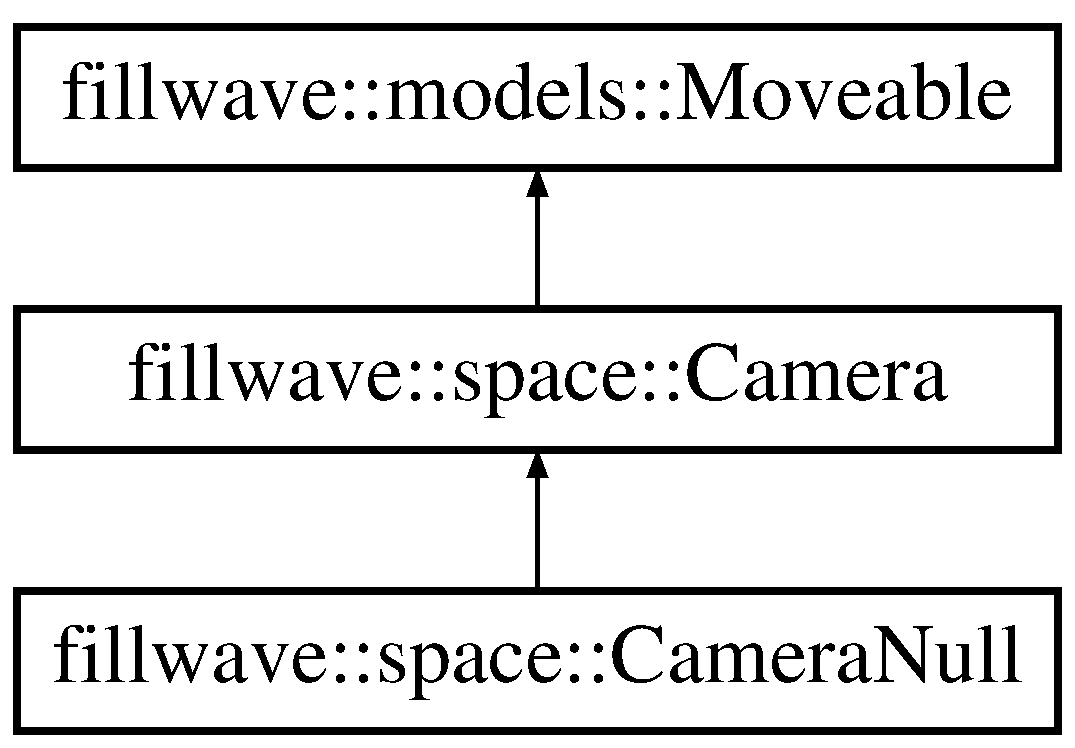
\includegraphics[height=3.000000cm]{classfillwave_1_1space_1_1CameraNull}
\end{center}
\end{figure}
\subsection*{Public Member Functions}
\begin{DoxyCompactItemize}
\item 
\hypertarget{classfillwave_1_1space_1_1CameraNull_a5166bbcf48ec9e4b7307e0a884060418}{}void {\bfseries update\+Projection} ()\label{classfillwave_1_1space_1_1CameraNull_a5166bbcf48ec9e4b7307e0a884060418}

\item 
\hypertarget{classfillwave_1_1space_1_1CameraNull_a8209d47b332935bbe48d9de9355daecb}{}G\+Lfloat {\bfseries get\+Projection\+Near\+Plane} ()\label{classfillwave_1_1space_1_1CameraNull_a8209d47b332935bbe48d9de9355daecb}

\item 
\hypertarget{classfillwave_1_1space_1_1CameraNull_aa2d4f17a7adf55046699b6a119fb5934}{}G\+Lfloat {\bfseries get\+Projection\+Far\+Plane} ()\label{classfillwave_1_1space_1_1CameraNull_aa2d4f17a7adf55046699b6a119fb5934}

\end{DoxyCompactItemize}
\subsection*{Additional Inherited Members}


\subsection{Detailed Description}
Not used. \hyperlink{classfillwave_1_1space_1_1Camera}{Camera} for which both projection and view matrices are always identities. 

The documentation for this class was generated from the following file\+:\begin{DoxyCompactItemize}
\item 
/home/filip/\+Projects/fillwave/inc/fillwave/space/Camera\+Null.\+h\end{DoxyCompactItemize}

\hypertarget{classfillwave_1_1space_1_1CameraOrthographic}{}\section{fillwave\+:\+:space\+:\+:Camera\+Orthographic Class Reference}
\label{classfillwave_1_1space_1_1CameraOrthographic}\index{fillwave\+::space\+::\+Camera\+Orthographic@{fillwave\+::space\+::\+Camera\+Orthographic}}


\hyperlink{classfillwave_1_1space_1_1Camera}{Camera} with Orthographic projection.  




{\ttfamily \#include $<$Camera\+Orthographic.\+h$>$}

Inheritance diagram for fillwave\+:\+:space\+:\+:Camera\+Orthographic\+:\begin{figure}[H]
\begin{center}
\leavevmode
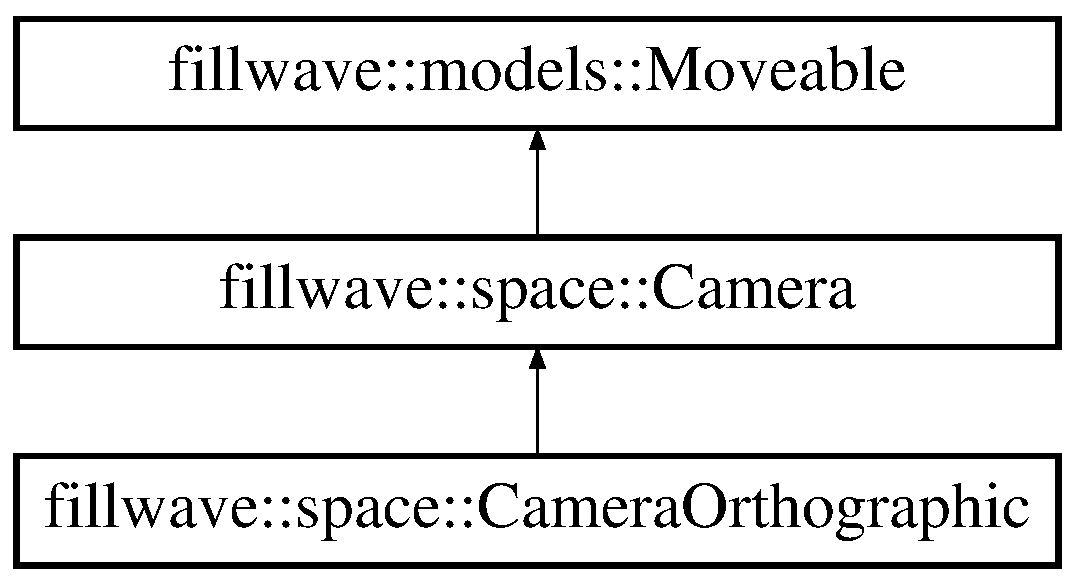
\includegraphics[height=3.000000cm]{classfillwave_1_1space_1_1CameraOrthographic}
\end{center}
\end{figure}
\subsection*{Public Member Functions}
\begin{DoxyCompactItemize}
\item 
\hypertarget{classfillwave_1_1space_1_1CameraOrthographic_abc1f9cd4da3014e662ee8f4da74461ef}{}{\bfseries Camera\+Orthographic} (glm\+::vec3 position, glm\+::quat rotation, G\+Lfloat left, G\+Lfloat right, G\+Lfloat bottom, G\+Lfloat top, G\+Lfloat near, G\+Lfloat far)\label{classfillwave_1_1space_1_1CameraOrthographic_abc1f9cd4da3014e662ee8f4da74461ef}

\item 
\hypertarget{classfillwave_1_1space_1_1CameraOrthographic_a9702d624e347c4f895ca382af2f5f887}{}void {\bfseries update\+Projection} ()\label{classfillwave_1_1space_1_1CameraOrthographic_a9702d624e347c4f895ca382af2f5f887}

\item 
\hypertarget{classfillwave_1_1space_1_1CameraOrthographic_af7f315b1986a462ca6b91b2b9905d757}{}G\+Lfloat {\bfseries get\+Projection\+Near\+Plane} ()\label{classfillwave_1_1space_1_1CameraOrthographic_af7f315b1986a462ca6b91b2b9905d757}

\item 
\hypertarget{classfillwave_1_1space_1_1CameraOrthographic_afef849479a96b786837c556ef978d672}{}G\+Lfloat {\bfseries get\+Projection\+Far\+Plane} ()\label{classfillwave_1_1space_1_1CameraOrthographic_afef849479a96b786837c556ef978d672}

\end{DoxyCompactItemize}
\subsection*{Additional Inherited Members}


\subsection{Detailed Description}
\hyperlink{classfillwave_1_1space_1_1Camera}{Camera} with Orthographic projection. 

The documentation for this class was generated from the following file\+:\begin{DoxyCompactItemize}
\item 
/home/filip/\+Projects/fillwave/inc/fillwave/space/Camera\+Orthographic.\+h\end{DoxyCompactItemize}

\hypertarget{classfillwave_1_1space_1_1CameraPerspective}{}\section{fillwave\+:\+:space\+:\+:Camera\+Perspective Class Reference}
\label{classfillwave_1_1space_1_1CameraPerspective}\index{fillwave\+::space\+::\+Camera\+Perspective@{fillwave\+::space\+::\+Camera\+Perspective}}


\hyperlink{classfillwave_1_1space_1_1Camera}{Camera} with perspective projection.  




{\ttfamily \#include $<$Camera\+Perspective.\+h$>$}

Inheritance diagram for fillwave\+:\+:space\+:\+:Camera\+Perspective\+:\begin{figure}[H]
\begin{center}
\leavevmode
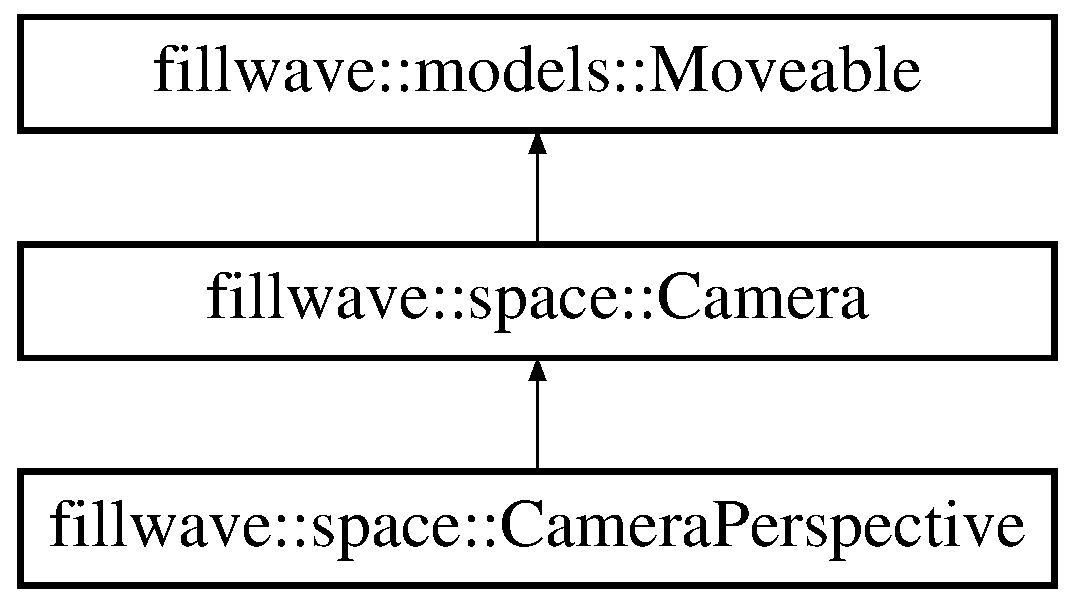
\includegraphics[height=3.000000cm]{classfillwave_1_1space_1_1CameraPerspective}
\end{center}
\end{figure}
\subsection*{Public Member Functions}
\begin{DoxyCompactItemize}
\item 
\hypertarget{classfillwave_1_1space_1_1CameraPerspective_ae296af21ba0b3a26a48b9e2568de0e15}{}{\bfseries Camera\+Perspective} (glm\+::vec3 position, glm\+::quat rotation, G\+Lfloat fovy=90, G\+Lfloat aspect\+Ratio=1, G\+Lfloat near\+Plane=0.\+01, G\+Lfloat far\+Plane=100.\+0)\label{classfillwave_1_1space_1_1CameraPerspective_ae296af21ba0b3a26a48b9e2568de0e15}

\item 
\hypertarget{classfillwave_1_1space_1_1CameraPerspective_a882ea7b48e8cefbf8f5ad636c957da9f}{}G\+Lfloat {\bfseries get\+Projection\+Fovy} ()\label{classfillwave_1_1space_1_1CameraPerspective_a882ea7b48e8cefbf8f5ad636c957da9f}

\item 
\hypertarget{classfillwave_1_1space_1_1CameraPerspective_a0dc1dcacc39c30875a61f43638b851e8}{}G\+Lfloat {\bfseries get\+Projection\+Aspect\+Ratio} ()\label{classfillwave_1_1space_1_1CameraPerspective_a0dc1dcacc39c30875a61f43638b851e8}

\item 
\hypertarget{classfillwave_1_1space_1_1CameraPerspective_adbd7c01df7c7bbc579d02c3213c40b74}{}G\+Lfloat {\bfseries get\+Projection\+Near\+Plane} ()\label{classfillwave_1_1space_1_1CameraPerspective_adbd7c01df7c7bbc579d02c3213c40b74}

\item 
\hypertarget{classfillwave_1_1space_1_1CameraPerspective_af943b9817dd8a2173ab9a59ff1c55592}{}G\+Lfloat {\bfseries get\+Projection\+Far\+Plane} ()\label{classfillwave_1_1space_1_1CameraPerspective_af943b9817dd8a2173ab9a59ff1c55592}

\item 
\hypertarget{classfillwave_1_1space_1_1CameraPerspective_a5bc53d77f61f11ec45879af4e68bd3b2}{}void {\bfseries set\+Projection\+Fovy} (G\+Lfloat fovy)\label{classfillwave_1_1space_1_1CameraPerspective_a5bc53d77f61f11ec45879af4e68bd3b2}

\item 
\hypertarget{classfillwave_1_1space_1_1CameraPerspective_a141fad001ae7ef1946145f8c5b9411cd}{}void {\bfseries set\+Projection\+Aspect\+Ratio} (G\+Lfloat aspect)\label{classfillwave_1_1space_1_1CameraPerspective_a141fad001ae7ef1946145f8c5b9411cd}

\item 
\hypertarget{classfillwave_1_1space_1_1CameraPerspective_adf96078566258ddf46643d1f1f0f13ef}{}void {\bfseries set\+Projection\+Near\+Plane} (G\+Lfloat near\+Plane)\label{classfillwave_1_1space_1_1CameraPerspective_adf96078566258ddf46643d1f1f0f13ef}

\item 
\hypertarget{classfillwave_1_1space_1_1CameraPerspective_a1feb81361eeb1c607f8a2b34169e73a4}{}void {\bfseries set\+Projection\+Far\+Plane} (G\+Lfloat far\+Plane)\label{classfillwave_1_1space_1_1CameraPerspective_a1feb81361eeb1c607f8a2b34169e73a4}

\item 
\hypertarget{classfillwave_1_1space_1_1CameraPerspective_ad9e09f2d1a77c00e69cb2369249ce357}{}void {\bfseries update\+Projection} ()\label{classfillwave_1_1space_1_1CameraPerspective_ad9e09f2d1a77c00e69cb2369249ce357}

\end{DoxyCompactItemize}
\subsection*{Additional Inherited Members}


\subsection{Detailed Description}
\hyperlink{classfillwave_1_1space_1_1Camera}{Camera} with perspective projection. 

The documentation for this class was generated from the following file\+:\begin{DoxyCompactItemize}
\item 
/home/filip/\+Projects/fillwave/inc/fillwave/space/Camera\+Perspective.\+h\end{DoxyCompactItemize}

\hypertarget{classfillwave_1_1animation_1_1Channel}{}\section{fillwave\+:\+:animation\+:\+:Channel Class Reference}
\label{classfillwave_1_1animation_1_1Channel}\index{fillwave\+::animation\+::\+Channel@{fillwave\+::animation\+::\+Channel}}


wrapper to assimp ai\+Node\+Anim$\ast$  




{\ttfamily \#include $<$Channel.\+h$>$}

\subsection*{Public Member Functions}
\begin{DoxyCompactItemize}
\item 
\hypertarget{classfillwave_1_1animation_1_1Channel_ab888f2f914596577a8db9e8ffd3402d8}{}{\bfseries Channel} (f\+Node\+Anim $\ast$assimp\+Channel)\label{classfillwave_1_1animation_1_1Channel_ab888f2f914596577a8db9e8ffd3402d8}

\end{DoxyCompactItemize}
\subsection*{Public Attributes}
\begin{DoxyCompactItemize}
\item 
\hypertarget{classfillwave_1_1animation_1_1Channel_a09662a0c98b28ddf31d51eb3b36b3197}{}std\+::string {\bfseries m\+Affected\+Node\+Name}\label{classfillwave_1_1animation_1_1Channel_a09662a0c98b28ddf31d51eb3b36b3197}

\item 
\hypertarget{classfillwave_1_1animation_1_1Channel_a4845f2bb5d2379d2d724aa12b4e256b1}{}std\+::vector$<$ \hyperlink{classfillwave_1_1animation_1_1Key}{Key}$<$ glm\+::vec3 $>$ $>$ {\bfseries m\+Keys\+Translation}\label{classfillwave_1_1animation_1_1Channel_a4845f2bb5d2379d2d724aa12b4e256b1}

\item 
\hypertarget{classfillwave_1_1animation_1_1Channel_a9378f708d1f62adc7270f18a5571f74f}{}std\+::vector$<$ \hyperlink{classfillwave_1_1animation_1_1Key}{Key}$<$ glm\+::quat $>$ $>$ {\bfseries m\+Keys\+Rotation}\label{classfillwave_1_1animation_1_1Channel_a9378f708d1f62adc7270f18a5571f74f}

\item 
\hypertarget{classfillwave_1_1animation_1_1Channel_a42ea94e79ed5ebc72c2c85c866d04139}{}std\+::vector$<$ \hyperlink{classfillwave_1_1animation_1_1Key}{Key}$<$ glm\+::vec3 $>$ $>$ {\bfseries m\+Keys\+Scaling}\label{classfillwave_1_1animation_1_1Channel_a42ea94e79ed5ebc72c2c85c866d04139}

\end{DoxyCompactItemize}


\subsection{Detailed Description}
wrapper to assimp ai\+Node\+Anim$\ast$ 

The documentation for this class was generated from the following file\+:\begin{DoxyCompactItemize}
\item 
/home/filip/\+Projects/fillwave/inc/fillwave/animation/Channel.\+h\end{DoxyCompactItemize}

\hypertarget{classfillwave_1_1actions_1_1CharacterEvent}{}\section{fillwave\+:\+:actions\+:\+:Character\+Event Struct Reference}
\label{classfillwave_1_1actions_1_1CharacterEvent}\index{fillwave\+::actions\+::\+Character\+Event@{fillwave\+::actions\+::\+Character\+Event}}


\hyperlink{classfillwave_1_1actions_1_1Event}{Event} introduced when the key is pressed.  




{\ttfamily \#include $<$Character\+Event.\+h$>$}

Inheritance diagram for fillwave\+:\+:actions\+:\+:Character\+Event\+:\begin{figure}[H]
\begin{center}
\leavevmode
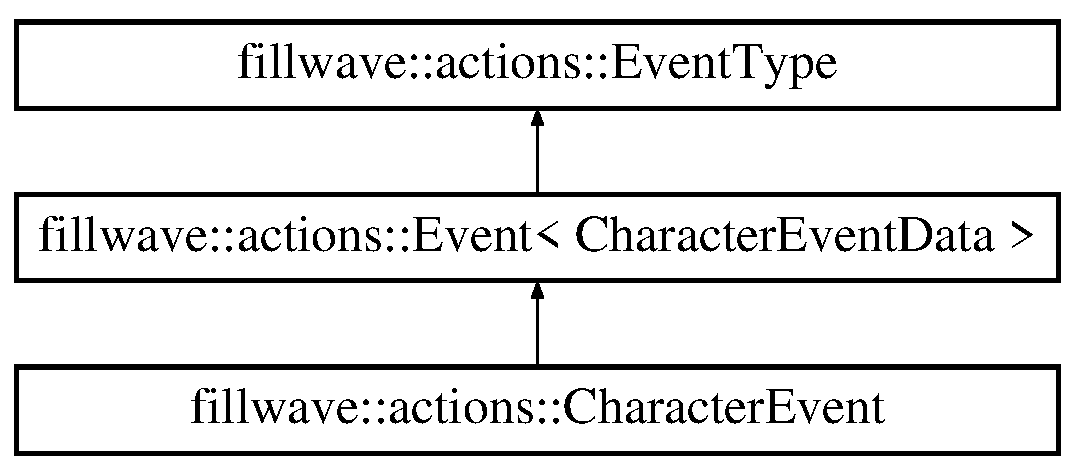
\includegraphics[height=3.000000cm]{classfillwave_1_1actions_1_1CharacterEvent}
\end{center}
\end{figure}
\subsection*{Public Member Functions}
\begin{DoxyCompactItemize}
\item 
\hypertarget{classfillwave_1_1actions_1_1CharacterEvent_acab3baf0d6290fbf51be493acd0af1a5}{}{\bfseries Character\+Event} (\hyperlink{structfillwave_1_1actions_1_1CharacterEventData}{Character\+Event\+Data} \&data)\label{classfillwave_1_1actions_1_1CharacterEvent_acab3baf0d6290fbf51be493acd0af1a5}

\end{DoxyCompactItemize}
\subsection*{Additional Inherited Members}


\subsection{Detailed Description}
\hyperlink{classfillwave_1_1actions_1_1Event}{Event} introduced when the key is pressed. 

The documentation for this struct was generated from the following file\+:\begin{DoxyCompactItemize}
\item 
/home/filip/\+Projects/fillwave/inc/fillwave/actions/Character\+Event.\+h\end{DoxyCompactItemize}

\hypertarget{structfillwave_1_1actions_1_1CharacterEventData}{}\section{fillwave\+:\+:actions\+:\+:Character\+Event\+Data Struct Reference}
\label{structfillwave_1_1actions_1_1CharacterEventData}\index{fillwave\+::actions\+::\+Character\+Event\+Data@{fillwave\+::actions\+::\+Character\+Event\+Data}}


\hyperlink{classfillwave_1_1actions_1_1Event}{Event} data structure to store the character.  




{\ttfamily \#include $<$Character\+Event.\+h$>$}

\subsection*{Public Attributes}
\begin{DoxyCompactItemize}
\item 
\hypertarget{structfillwave_1_1actions_1_1CharacterEventData_a378b8eb5aa654104714acd4101f57162}{}unsigned int {\bfseries character}\label{structfillwave_1_1actions_1_1CharacterEventData_a378b8eb5aa654104714acd4101f57162}

\item 
\hypertarget{structfillwave_1_1actions_1_1CharacterEventData_a2067f02a01602c7f40d5094eb089f550}{}const e\+Event\+Type {\bfseries type} = e\+Event\+Type\+::character\label{structfillwave_1_1actions_1_1CharacterEventData_a2067f02a01602c7f40d5094eb089f550}

\end{DoxyCompactItemize}


\subsection{Detailed Description}
\hyperlink{classfillwave_1_1actions_1_1Event}{Event} data structure to store the character. 

The documentation for this struct was generated from the following file\+:\begin{DoxyCompactItemize}
\item 
/home/filip/\+Projects/fillwave/inc/fillwave/actions/Character\+Event.\+h\end{DoxyCompactItemize}

\hypertarget{classfillwave_1_1actions_1_1CharacterModsEvent}{}\section{fillwave\+:\+:actions\+:\+:Character\+Mods\+Event Struct Reference}
\label{classfillwave_1_1actions_1_1CharacterModsEvent}\index{fillwave\+::actions\+::\+Character\+Mods\+Event@{fillwave\+::actions\+::\+Character\+Mods\+Event}}


\hyperlink{classfillwave_1_1actions_1_1Event}{Event} introduced when the key is pressed.  




{\ttfamily \#include $<$Character\+Mods\+Event.\+h$>$}

Inheritance diagram for fillwave\+:\+:actions\+:\+:Character\+Mods\+Event\+:\begin{figure}[H]
\begin{center}
\leavevmode
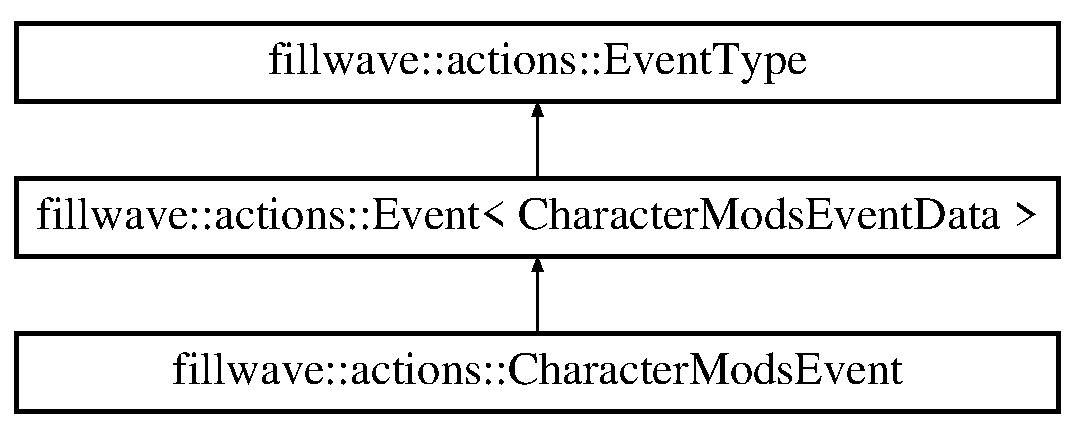
\includegraphics[height=3.000000cm]{classfillwave_1_1actions_1_1CharacterModsEvent}
\end{center}
\end{figure}
\subsection*{Public Member Functions}
\begin{DoxyCompactItemize}
\item 
\hypertarget{classfillwave_1_1actions_1_1CharacterModsEvent_ae4695d3a663f83a99b9962b7b2d89303}{}{\bfseries Character\+Mods\+Event} (\hyperlink{structfillwave_1_1actions_1_1CharacterModsEventData}{Character\+Mods\+Event\+Data} \&data)\label{classfillwave_1_1actions_1_1CharacterModsEvent_ae4695d3a663f83a99b9962b7b2d89303}

\end{DoxyCompactItemize}
\subsection*{Additional Inherited Members}


\subsection{Detailed Description}
\hyperlink{classfillwave_1_1actions_1_1Event}{Event} introduced when the key is pressed. 

The documentation for this struct was generated from the following file\+:\begin{DoxyCompactItemize}
\item 
/home/filip/\+Projects/fillwave/inc/fillwave/actions/Character\+Mods\+Event.\+h\end{DoxyCompactItemize}

\hypertarget{structfillwave_1_1actions_1_1CharacterModsEventData}{}\section{fillwave\+:\+:actions\+:\+:Character\+Mods\+Event\+Data Struct Reference}
\label{structfillwave_1_1actions_1_1CharacterModsEventData}\index{fillwave\+::actions\+::\+Character\+Mods\+Event\+Data@{fillwave\+::actions\+::\+Character\+Mods\+Event\+Data}}


\hyperlink{classfillwave_1_1actions_1_1Event}{Event} data structure to store the character together with modifier keys.  




{\ttfamily \#include $<$Character\+Mods\+Event.\+h$>$}

\subsection*{Public Attributes}
\begin{DoxyCompactItemize}
\item 
\hypertarget{structfillwave_1_1actions_1_1CharacterModsEventData_a8694e8dc9f263e01e5f2cc81e0100d38}{}unsigned int {\bfseries character}\label{structfillwave_1_1actions_1_1CharacterModsEventData_a8694e8dc9f263e01e5f2cc81e0100d38}

\item 
\hypertarget{structfillwave_1_1actions_1_1CharacterModsEventData_a4cf040017ffcef283873071fdfbf4ea9}{}int {\bfseries modsifier\+Keys}\label{structfillwave_1_1actions_1_1CharacterModsEventData_a4cf040017ffcef283873071fdfbf4ea9}

\item 
\hypertarget{structfillwave_1_1actions_1_1CharacterModsEventData_a0562ffc2dfbb6848510ec9337a8f6fc7}{}const e\+Event\+Type {\bfseries type} = e\+Event\+Type\+::character\+Mods\label{structfillwave_1_1actions_1_1CharacterModsEventData_a0562ffc2dfbb6848510ec9337a8f6fc7}

\end{DoxyCompactItemize}


\subsection{Detailed Description}
\hyperlink{classfillwave_1_1actions_1_1Event}{Event} data structure to store the character together with modifier keys. 

The documentation for this struct was generated from the following file\+:\begin{DoxyCompactItemize}
\item 
/home/filip/\+Projects/fillwave/inc/fillwave/actions/Character\+Mods\+Event.\+h\end{DoxyCompactItemize}

\hypertarget{classfillwave_1_1effects_1_1ClockwiseDrawEffect}{}\section{fillwave\+:\+:effects\+:\+:Clockwise\+Draw\+Effect Class Reference}
\label{classfillwave_1_1effects_1_1ClockwiseDrawEffect}\index{fillwave\+::effects\+::\+Clockwise\+Draw\+Effect@{fillwave\+::effects\+::\+Clockwise\+Draw\+Effect}}


\hyperlink{classfillwave_1_1effects_1_1Effect}{Effect} to draw an opposite face of each mesh.  




{\ttfamily \#include $<$Clockwise\+Draw\+Effect.\+h$>$}

Inheritance diagram for fillwave\+:\+:effects\+:\+:Clockwise\+Draw\+Effect\+:\begin{figure}[H]
\begin{center}
\leavevmode
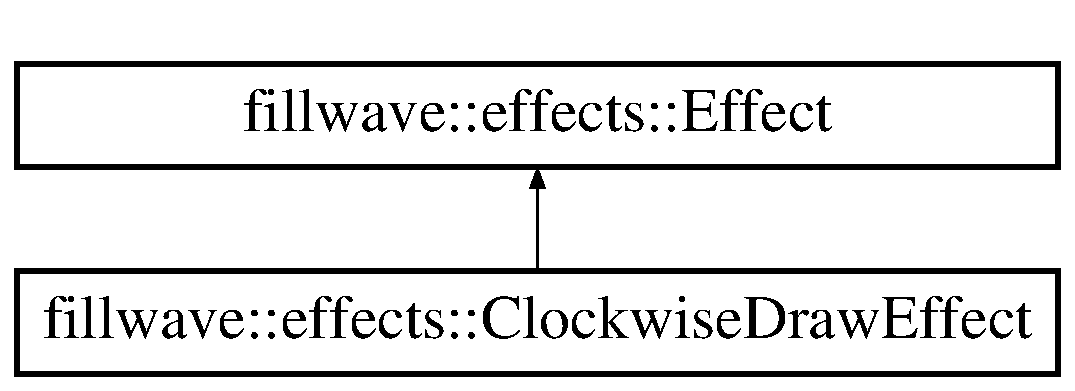
\includegraphics[height=2.000000cm]{classfillwave_1_1effects_1_1ClockwiseDrawEffect}
\end{center}
\end{figure}
\subsection*{Public Member Functions}
\begin{DoxyCompactItemize}
\item 
void \hyperlink{classfillwave_1_1effects_1_1ClockwiseDrawEffect_a0aa6fa5faf4d87d9defc4039f17fe615}{pre\+Draw\+Action} (\hyperlink{classfillwave_1_1core_1_1Program}{core\+::\+Program} $\ast$program)
\begin{DoxyCompactList}\small\item\em virtual\+: defines action to be done just before the draw. \end{DoxyCompactList}\item 
void \hyperlink{classfillwave_1_1effects_1_1ClockwiseDrawEffect_a1565a96fe8744c414bfb0a082adce1d3}{post\+Draw\+Action} (\hyperlink{classfillwave_1_1core_1_1Program}{core\+::\+Program} $\ast$program)
\begin{DoxyCompactList}\small\item\em virtual\+: defines action to be done just after the draw. \end{DoxyCompactList}\item 
void \hyperlink{classfillwave_1_1effects_1_1ClockwiseDrawEffect_af496a94f611f378e365f0f56130201a9}{stop\+Action} (\hyperlink{classfillwave_1_1core_1_1Program}{core\+::\+Program} $\ast$program)
\begin{DoxyCompactList}\small\item\em virtual\+: defines action to be done when the effect is stopped. \end{DoxyCompactList}\item 
void \hyperlink{classfillwave_1_1effects_1_1ClockwiseDrawEffect_a793f6c4d14c18bc366a17892d7764da8}{start\+Action} (\hyperlink{classfillwave_1_1core_1_1Program}{core\+::\+Program} $\ast$program)
\begin{DoxyCompactList}\small\item\em virtual\+: defines action to be done when the effect is started. \end{DoxyCompactList}\end{DoxyCompactItemize}


\subsection{Detailed Description}
\hyperlink{classfillwave_1_1effects_1_1Effect}{Effect} to draw an opposite face of each mesh. 

\subsection{Member Function Documentation}
\hypertarget{classfillwave_1_1effects_1_1ClockwiseDrawEffect_a1565a96fe8744c414bfb0a082adce1d3}{}\index{fillwave\+::effects\+::\+Clockwise\+Draw\+Effect@{fillwave\+::effects\+::\+Clockwise\+Draw\+Effect}!post\+Draw\+Action@{post\+Draw\+Action}}
\index{post\+Draw\+Action@{post\+Draw\+Action}!fillwave\+::effects\+::\+Clockwise\+Draw\+Effect@{fillwave\+::effects\+::\+Clockwise\+Draw\+Effect}}
\subsubsection[{post\+Draw\+Action}]{\setlength{\rightskip}{0pt plus 5cm}void fillwave\+::effects\+::\+Clockwise\+Draw\+Effect\+::post\+Draw\+Action (
\begin{DoxyParamCaption}
\item[{{\bf core\+::\+Program} $\ast$}]{program}
\end{DoxyParamCaption}
)\hspace{0.3cm}{\ttfamily [virtual]}}\label{classfillwave_1_1effects_1_1ClockwiseDrawEffect_a1565a96fe8744c414bfb0a082adce1d3}


virtual\+: defines action to be done just after the draw. 

post\+Draw\+Action 

Implements \hyperlink{classfillwave_1_1effects_1_1Effect_ae01123633990402e11226c4d9a2dce1b}{fillwave\+::effects\+::\+Effect}.

\hypertarget{classfillwave_1_1effects_1_1ClockwiseDrawEffect_a0aa6fa5faf4d87d9defc4039f17fe615}{}\index{fillwave\+::effects\+::\+Clockwise\+Draw\+Effect@{fillwave\+::effects\+::\+Clockwise\+Draw\+Effect}!pre\+Draw\+Action@{pre\+Draw\+Action}}
\index{pre\+Draw\+Action@{pre\+Draw\+Action}!fillwave\+::effects\+::\+Clockwise\+Draw\+Effect@{fillwave\+::effects\+::\+Clockwise\+Draw\+Effect}}
\subsubsection[{pre\+Draw\+Action}]{\setlength{\rightskip}{0pt plus 5cm}void fillwave\+::effects\+::\+Clockwise\+Draw\+Effect\+::pre\+Draw\+Action (
\begin{DoxyParamCaption}
\item[{{\bf core\+::\+Program} $\ast$}]{program}
\end{DoxyParamCaption}
)\hspace{0.3cm}{\ttfamily [virtual]}}\label{classfillwave_1_1effects_1_1ClockwiseDrawEffect_a0aa6fa5faf4d87d9defc4039f17fe615}


virtual\+: defines action to be done just before the draw. 

pre\+Draw\+Action 

Implements \hyperlink{classfillwave_1_1effects_1_1Effect_a99c243cb10f504bfc6193e5e81926920}{fillwave\+::effects\+::\+Effect}.

\hypertarget{classfillwave_1_1effects_1_1ClockwiseDrawEffect_a793f6c4d14c18bc366a17892d7764da8}{}\index{fillwave\+::effects\+::\+Clockwise\+Draw\+Effect@{fillwave\+::effects\+::\+Clockwise\+Draw\+Effect}!start\+Action@{start\+Action}}
\index{start\+Action@{start\+Action}!fillwave\+::effects\+::\+Clockwise\+Draw\+Effect@{fillwave\+::effects\+::\+Clockwise\+Draw\+Effect}}
\subsubsection[{start\+Action}]{\setlength{\rightskip}{0pt plus 5cm}void fillwave\+::effects\+::\+Clockwise\+Draw\+Effect\+::start\+Action (
\begin{DoxyParamCaption}
\item[{{\bf core\+::\+Program} $\ast$}]{program}
\end{DoxyParamCaption}
)\hspace{0.3cm}{\ttfamily [virtual]}}\label{classfillwave_1_1effects_1_1ClockwiseDrawEffect_a793f6c4d14c18bc366a17892d7764da8}


virtual\+: defines action to be done when the effect is started. 

start\+Action 

Implements \hyperlink{classfillwave_1_1effects_1_1Effect_af0a4aa202fa7201cd19cedf71f6c682a}{fillwave\+::effects\+::\+Effect}.

\hypertarget{classfillwave_1_1effects_1_1ClockwiseDrawEffect_af496a94f611f378e365f0f56130201a9}{}\index{fillwave\+::effects\+::\+Clockwise\+Draw\+Effect@{fillwave\+::effects\+::\+Clockwise\+Draw\+Effect}!stop\+Action@{stop\+Action}}
\index{stop\+Action@{stop\+Action}!fillwave\+::effects\+::\+Clockwise\+Draw\+Effect@{fillwave\+::effects\+::\+Clockwise\+Draw\+Effect}}
\subsubsection[{stop\+Action}]{\setlength{\rightskip}{0pt plus 5cm}void fillwave\+::effects\+::\+Clockwise\+Draw\+Effect\+::stop\+Action (
\begin{DoxyParamCaption}
\item[{{\bf core\+::\+Program} $\ast$}]{program}
\end{DoxyParamCaption}
)\hspace{0.3cm}{\ttfamily [virtual]}}\label{classfillwave_1_1effects_1_1ClockwiseDrawEffect_af496a94f611f378e365f0f56130201a9}


virtual\+: defines action to be done when the effect is stopped. 

stop\+Action 

Implements \hyperlink{classfillwave_1_1effects_1_1Effect_aed8c053b5798cbbc6668117989d18ead}{fillwave\+::effects\+::\+Effect}.



The documentation for this class was generated from the following file\+:\begin{DoxyCompactItemize}
\item 
/home/filip/\+Projects/fillwave/inc/fillwave/effects/Clockwise\+Draw\+Effect.\+h\end{DoxyCompactItemize}

\hypertarget{classfillwave_1_1core_1_1ConditionalRender}{}\section{fillwave\+:\+:core\+:\+:Conditional\+Render Class Reference}
\label{classfillwave_1_1core_1_1ConditionalRender}\index{fillwave\+::core\+::\+Conditional\+Render@{fillwave\+::core\+::\+Conditional\+Render}}


Operation of rendering only meshes passing the occlusion test.  




{\ttfamily \#include $<$Conditional\+Render.\+h$>$}

\subsection*{Public Member Functions}
\begin{DoxyCompactItemize}
\item 
\hyperlink{classfillwave_1_1core_1_1ConditionalRender_a405d055bd9b4d4833976f0a906af9df6}{Conditional\+Render} (G\+Lenum mode)
\begin{DoxyCompactList}\small\item\em Specifies the conditional rendering pass mode. \end{DoxyCompactList}\item 
\hypertarget{classfillwave_1_1core_1_1ConditionalRender_a892c070d065d80eb66396a6090b01a3c}{}void {\bfseries begin} (G\+Luint querry\+I\+D)\label{classfillwave_1_1core_1_1ConditionalRender_a892c070d065d80eb66396a6090b01a3c}

\item 
\hypertarget{classfillwave_1_1core_1_1ConditionalRender_ab3cd5b2fd6cbcb2953c93bc10d04cd6d}{}void {\bfseries end} ()\label{classfillwave_1_1core_1_1ConditionalRender_ab3cd5b2fd6cbcb2953c93bc10d04cd6d}

\end{DoxyCompactItemize}


\subsection{Detailed Description}
Operation of rendering only meshes passing the occlusion test. 

\subsection{Constructor \& Destructor Documentation}
\hypertarget{classfillwave_1_1core_1_1ConditionalRender_a405d055bd9b4d4833976f0a906af9df6}{}\index{fillwave\+::core\+::\+Conditional\+Render@{fillwave\+::core\+::\+Conditional\+Render}!Conditional\+Render@{Conditional\+Render}}
\index{Conditional\+Render@{Conditional\+Render}!fillwave\+::core\+::\+Conditional\+Render@{fillwave\+::core\+::\+Conditional\+Render}}
\subsubsection[{Conditional\+Render}]{\setlength{\rightskip}{0pt plus 5cm}fillwave\+::core\+::\+Conditional\+Render\+::\+Conditional\+Render (
\begin{DoxyParamCaption}
\item[{G\+Lenum}]{mode}
\end{DoxyParamCaption}
)}\label{classfillwave_1_1core_1_1ConditionalRender_a405d055bd9b4d4833976f0a906af9df6}


Specifies the conditional rendering pass mode. 


\begin{DoxyParams}{Parameters}
{\em Possible} & modes\+: G\+L\+\_\+\+Q\+U\+E\+R\+Y\+\_\+\+W\+A\+I\+T, G\+L\+\_\+\+Q\+U\+E\+R\+Y\+\_\+\+N\+O\+\_\+\+W\+A\+I\+T, G\+L\+\_\+\+Q\+U\+E\+R\+Y\+\_\+\+B\+Y\+\_\+\+R\+E\+G\+I\+O\+N\+\_\+\+W\+A\+I\+T, G\+L\+\_\+\+Q\+U\+E\+R\+Y\+\_\+\+B\+Y\+\_\+\+R\+E\+G\+I\+O\+N\+\_\+\+N\+O\+\_\+\+W\+A\+I\+T, \\
\hline
\end{DoxyParams}


The documentation for this class was generated from the following file\+:\begin{DoxyCompactItemize}
\item 
/home/filip/\+Projects/fillwave/inc/fillwave/core/operations/Conditional\+Render.\+h\end{DoxyCompactItemize}

\hypertarget{structfillwave_1_1space_1_1CullingBox}{}\section{fillwave\+:\+:space\+:\+:Culling\+Box Class Reference}
\label{structfillwave_1_1space_1_1CullingBox}\index{fillwave\+::space\+::\+Culling\+Box@{fillwave\+::space\+::\+Culling\+Box}}


Stores culling box parameters for Orthographic projection.  




{\ttfamily \#include $<$Camera\+Orthographic.\+h$>$}

\subsection*{Public Attributes}
\begin{DoxyCompactItemize}
\item 
\hypertarget{structfillwave_1_1space_1_1CullingBox_a0da977e177698c82a007e7261229a024}{}G\+Lfloat {\bfseries m\+Projection\+Left}\label{structfillwave_1_1space_1_1CullingBox_a0da977e177698c82a007e7261229a024}

\item 
\hypertarget{structfillwave_1_1space_1_1CullingBox_a9cb0a157a0f85d9a30cec6e7f3ce4cc9}{}G\+Lfloat {\bfseries m\+Projection\+Right}\label{structfillwave_1_1space_1_1CullingBox_a9cb0a157a0f85d9a30cec6e7f3ce4cc9}

\item 
\hypertarget{structfillwave_1_1space_1_1CullingBox_a7664d25151a317eac48fe9bc480de2dd}{}G\+Lfloat {\bfseries m\+Projection\+Bottom}\label{structfillwave_1_1space_1_1CullingBox_a7664d25151a317eac48fe9bc480de2dd}

\item 
\hypertarget{structfillwave_1_1space_1_1CullingBox_a35be2f6d1e2f12fb0eb01512642afa94}{}G\+Lfloat {\bfseries m\+Projection\+Top}\label{structfillwave_1_1space_1_1CullingBox_a35be2f6d1e2f12fb0eb01512642afa94}

\item 
\hypertarget{structfillwave_1_1space_1_1CullingBox_a3e01d5a122c158400cb2b7225f07dfd4}{}G\+Lfloat {\bfseries m\+Projection\+Near}\label{structfillwave_1_1space_1_1CullingBox_a3e01d5a122c158400cb2b7225f07dfd4}

\item 
\hypertarget{structfillwave_1_1space_1_1CullingBox_afe329167202cfbe485f3e095c2589ad6}{}G\+Lfloat {\bfseries m\+Projection\+Far}\label{structfillwave_1_1space_1_1CullingBox_afe329167202cfbe485f3e095c2589ad6}

\end{DoxyCompactItemize}


\subsection{Detailed Description}
Stores culling box parameters for Orthographic projection. 

The documentation for this class was generated from the following file\+:\begin{DoxyCompactItemize}
\item 
/home/filip/\+Projects/fillwave/inc/fillwave/space/Camera\+Orthographic.\+h\end{DoxyCompactItemize}

\hypertarget{classfillwave_1_1particles_1_1Cursor}{}\section{fillwave\+:\+:particles\+:\+:Cursor Class Reference}
\label{classfillwave_1_1particles_1_1Cursor}\index{fillwave\+::particles\+::\+Cursor@{fillwave\+::particles\+::\+Cursor}}


\hyperlink{classfillwave_1_1particles_1_1Impostor}{Impostor} to handle custom cursor instead of the standard one.  




{\ttfamily \#include $<$Cursor.\+h$>$}

Inheritance diagram for fillwave\+:\+:particles\+:\+:Cursor\+:\begin{figure}[H]
\begin{center}
\leavevmode
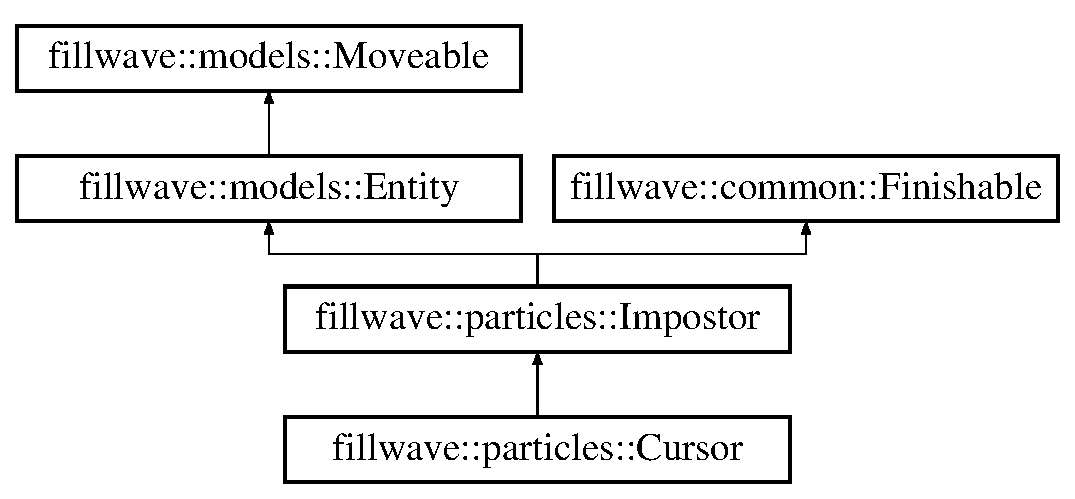
\includegraphics[height=4.000000cm]{classfillwave_1_1particles_1_1Cursor}
\end{center}
\end{figure}
\subsection*{Public Member Functions}
\begin{DoxyCompactItemize}
\item 
\hypertarget{classfillwave_1_1particles_1_1Cursor_a0ebc166e519fc14f589b2616c46cfa65}{}{\bfseries Cursor} (\hyperlink{classfillwave_1_1Engine}{Engine} $\ast$engine, p\+Texture texture)\label{classfillwave_1_1particles_1_1Cursor_a0ebc166e519fc14f589b2616c46cfa65}

\item 
\hypertarget{classfillwave_1_1particles_1_1Cursor_abc656ac436d96f3292bdd70698e1e262}{}void {\bfseries move} (glm\+::vec2 position)\label{classfillwave_1_1particles_1_1Cursor_abc656ac436d96f3292bdd70698e1e262}

\item 
\hypertarget{classfillwave_1_1particles_1_1Cursor_af80784f58512b6f59ef618a67d52277e}{}void {\bfseries draw} ()\label{classfillwave_1_1particles_1_1Cursor_af80784f58512b6f59ef618a67d52277e}

\end{DoxyCompactItemize}
\subsection*{Additional Inherited Members}


\subsection{Detailed Description}
\hyperlink{classfillwave_1_1particles_1_1Impostor}{Impostor} to handle custom cursor instead of the standard one. 

The documentation for this class was generated from the following file\+:\begin{DoxyCompactItemize}
\item 
/home/filip/\+Projects/fillwave/inc/fillwave/particles/Cursor.\+h\end{DoxyCompactItemize}

\hypertarget{classfillwave_1_1actions_1_1CursorEnterEvent}{}\section{fillwave\+:\+:actions\+:\+:Cursor\+Enter\+Event Struct Reference}
\label{classfillwave_1_1actions_1_1CursorEnterEvent}\index{fillwave\+::actions\+::\+Cursor\+Enter\+Event@{fillwave\+::actions\+::\+Cursor\+Enter\+Event}}


\hyperlink{classfillwave_1_1actions_1_1Event}{Event} introduced when cursor enters the window.  




{\ttfamily \#include $<$Cursor\+Enter\+Event.\+h$>$}

Inheritance diagram for fillwave\+:\+:actions\+:\+:Cursor\+Enter\+Event\+:\begin{figure}[H]
\begin{center}
\leavevmode
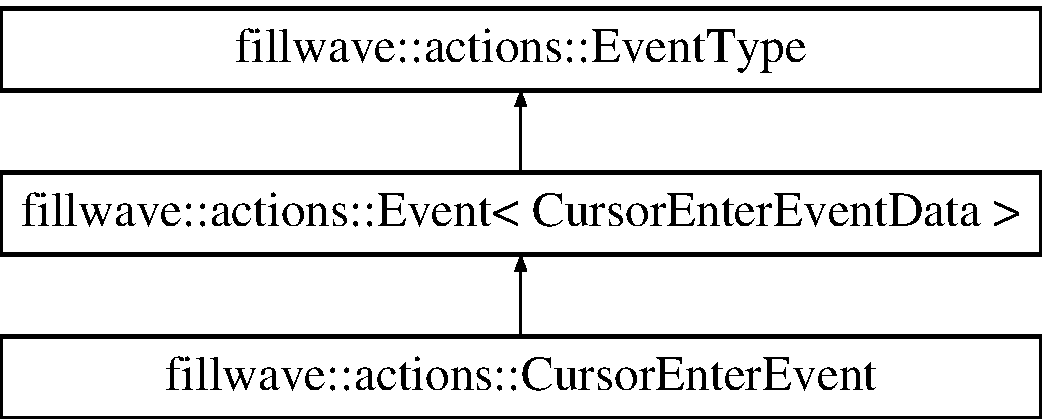
\includegraphics[height=3.000000cm]{classfillwave_1_1actions_1_1CursorEnterEvent}
\end{center}
\end{figure}
\subsection*{Public Member Functions}
\begin{DoxyCompactItemize}
\item 
\hypertarget{classfillwave_1_1actions_1_1CursorEnterEvent_a695cbbb66348b813642b3ba27283ae59}{}{\bfseries Cursor\+Enter\+Event} (\hyperlink{structfillwave_1_1actions_1_1CursorEnterEventData}{Cursor\+Enter\+Event\+Data} \&data)\label{classfillwave_1_1actions_1_1CursorEnterEvent_a695cbbb66348b813642b3ba27283ae59}

\end{DoxyCompactItemize}
\subsection*{Additional Inherited Members}


\subsection{Detailed Description}
\hyperlink{classfillwave_1_1actions_1_1Event}{Event} introduced when cursor enters the window. 

The documentation for this struct was generated from the following file\+:\begin{DoxyCompactItemize}
\item 
/home/filip/\+Projects/fillwave/inc/fillwave/actions/Cursor\+Enter\+Event.\+h\end{DoxyCompactItemize}

\hypertarget{structfillwave_1_1actions_1_1CursorEnterEventData}{}\section{fillwave\+:\+:actions\+:\+:Cursor\+Enter\+Event\+Data Struct Reference}
\label{structfillwave_1_1actions_1_1CursorEnterEventData}\index{fillwave\+::actions\+::\+Cursor\+Enter\+Event\+Data@{fillwave\+::actions\+::\+Cursor\+Enter\+Event\+Data}}


\hyperlink{classfillwave_1_1actions_1_1Event}{Event} data structure to store the Cursor\+Entered/\+Cursor\+Leaved data.  




{\ttfamily \#include $<$Cursor\+Enter\+Event.\+h$>$}

\subsection*{Public Attributes}
\begin{DoxyCompactItemize}
\item 
\hypertarget{structfillwave_1_1actions_1_1CursorEnterEventData_a524188b951d7bfb1b7a4d19a801d8f9f}{}int {\bfseries direction}\label{structfillwave_1_1actions_1_1CursorEnterEventData_a524188b951d7bfb1b7a4d19a801d8f9f}

\item 
\hypertarget{structfillwave_1_1actions_1_1CursorEnterEventData_a308768b426b03c0d2ae0b0293ad77edb}{}const e\+Event\+Type {\bfseries type} = e\+Event\+Type\+::cursor\+Enter\label{structfillwave_1_1actions_1_1CursorEnterEventData_a308768b426b03c0d2ae0b0293ad77edb}

\end{DoxyCompactItemize}


\subsection{Detailed Description}
\hyperlink{classfillwave_1_1actions_1_1Event}{Event} data structure to store the Cursor\+Entered/\+Cursor\+Leaved data. 

The documentation for this struct was generated from the following file\+:\begin{DoxyCompactItemize}
\item 
/home/filip/\+Projects/fillwave/inc/fillwave/actions/Cursor\+Enter\+Event.\+h\end{DoxyCompactItemize}

\hypertarget{classfillwave_1_1actions_1_1CursorPositionEvent}{}\section{fillwave\+:\+:actions\+:\+:Cursor\+Position\+Event Struct Reference}
\label{classfillwave_1_1actions_1_1CursorPositionEvent}\index{fillwave\+::actions\+::\+Cursor\+Position\+Event@{fillwave\+::actions\+::\+Cursor\+Position\+Event}}


\hyperlink{classfillwave_1_1actions_1_1Event}{Event} introduced when cursor position was changed.  




{\ttfamily \#include $<$Cursor\+Position\+Event.\+h$>$}

Inheritance diagram for fillwave\+:\+:actions\+:\+:Cursor\+Position\+Event\+:\begin{figure}[H]
\begin{center}
\leavevmode
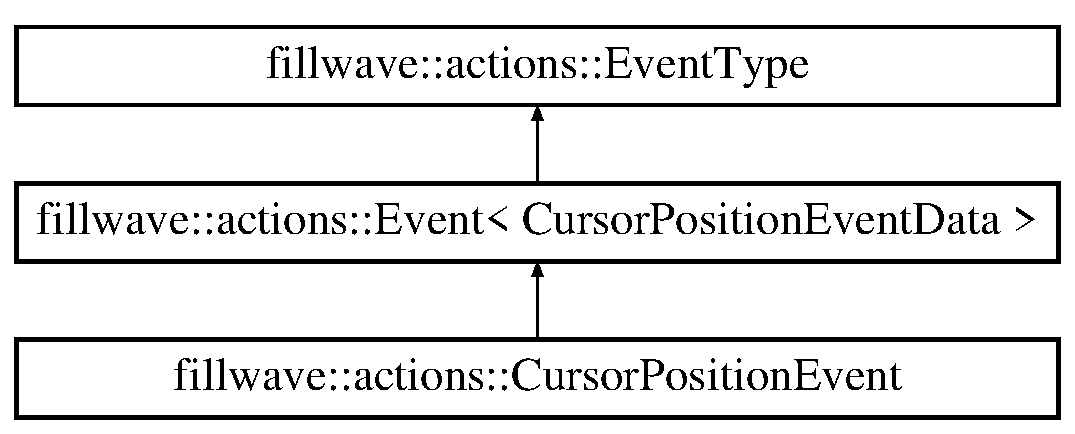
\includegraphics[height=3.000000cm]{classfillwave_1_1actions_1_1CursorPositionEvent}
\end{center}
\end{figure}
\subsection*{Public Member Functions}
\begin{DoxyCompactItemize}
\item 
\hypertarget{classfillwave_1_1actions_1_1CursorPositionEvent_a9bad24f2271b3c9e0943c472c98a5002}{}{\bfseries Cursor\+Position\+Event} (\hyperlink{structfillwave_1_1actions_1_1CursorPositionEventData}{Cursor\+Position\+Event\+Data} \&data)\label{classfillwave_1_1actions_1_1CursorPositionEvent_a9bad24f2271b3c9e0943c472c98a5002}

\end{DoxyCompactItemize}
\subsection*{Additional Inherited Members}


\subsection{Detailed Description}
\hyperlink{classfillwave_1_1actions_1_1Event}{Event} introduced when cursor position was changed. 

The documentation for this struct was generated from the following file\+:\begin{DoxyCompactItemize}
\item 
/home/filip/\+Projects/fillwave/inc/fillwave/actions/Cursor\+Position\+Event.\+h\end{DoxyCompactItemize}

\hypertarget{structfillwave_1_1actions_1_1CursorPositionEventData}{}\section{fillwave\+:\+:actions\+:\+:Cursor\+Position\+Event\+Data Struct Reference}
\label{structfillwave_1_1actions_1_1CursorPositionEventData}\index{fillwave\+::actions\+::\+Cursor\+Position\+Event\+Data@{fillwave\+::actions\+::\+Cursor\+Position\+Event\+Data}}


\hyperlink{classfillwave_1_1actions_1_1Event}{Event} data structure to store the cursor position.  




{\ttfamily \#include $<$Cursor\+Position\+Event.\+h$>$}

\subsection*{Public Attributes}
\begin{DoxyCompactItemize}
\item 
\hypertarget{structfillwave_1_1actions_1_1CursorPositionEventData_a2288026e8ab47bdbb1d161d03dfe70e6}{}double {\bfseries x\+Position}\label{structfillwave_1_1actions_1_1CursorPositionEventData_a2288026e8ab47bdbb1d161d03dfe70e6}

\item 
\hypertarget{structfillwave_1_1actions_1_1CursorPositionEventData_ac28fd3e33ba694248f8f9f024083e85e}{}double {\bfseries y\+Position}\label{structfillwave_1_1actions_1_1CursorPositionEventData_ac28fd3e33ba694248f8f9f024083e85e}

\item 
\hypertarget{structfillwave_1_1actions_1_1CursorPositionEventData_af764853b95496bdfd47a1019a5af8a46}{}const e\+Event\+Type {\bfseries type} = e\+Event\+Type\+::cursor\+Position\label{structfillwave_1_1actions_1_1CursorPositionEventData_af764853b95496bdfd47a1019a5af8a46}

\end{DoxyCompactItemize}


\subsection{Detailed Description}
\hyperlink{classfillwave_1_1actions_1_1Event}{Event} data structure to store the cursor position. 

The documentation for this struct was generated from the following file\+:\begin{DoxyCompactItemize}
\item 
/home/filip/\+Projects/fillwave/inc/fillwave/actions/Cursor\+Position\+Event.\+h\end{DoxyCompactItemize}

\hypertarget{classfillwave_1_1Debugger}{}\section{fillwave\+:\+:Debugger Class Reference}
\label{classfillwave_1_1Debugger}\index{fillwave\+::\+Debugger@{fillwave\+::\+Debugger}}


Fillwave debugger.  




{\ttfamily \#include $<$Debugger.\+h$>$}

Inheritance diagram for fillwave\+:\+:Debugger\+:\begin{figure}[H]
\begin{center}
\leavevmode
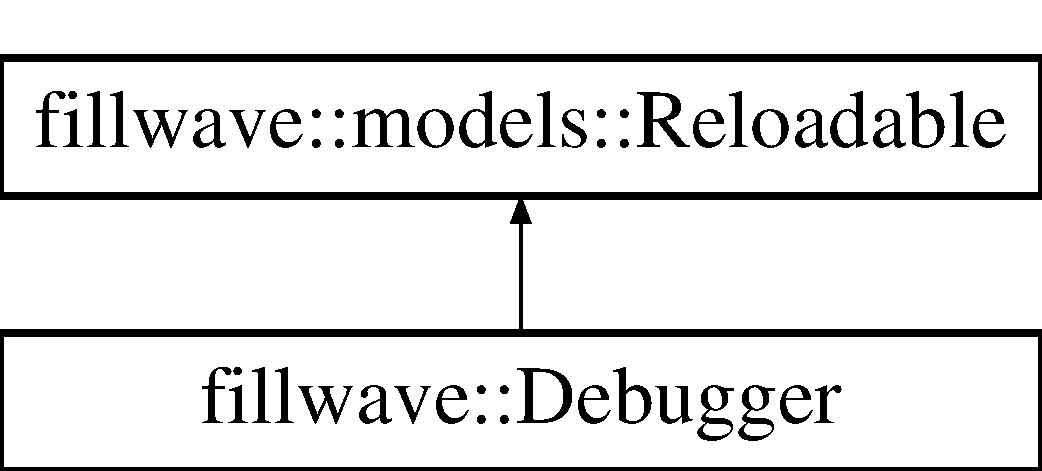
\includegraphics[height=2.000000cm]{classfillwave_1_1Debugger}
\end{center}
\end{figure}
\subsection*{Public Member Functions}
\begin{DoxyCompactItemize}
\item 
\hypertarget{classfillwave_1_1Debugger_a916a59a8b573be238f26626a3dd3e0df}{}{\bfseries Debugger} (\hyperlink{classfillwave_1_1Engine}{Engine} $\ast$engine)\label{classfillwave_1_1Debugger_a916a59a8b573be238f26626a3dd3e0df}

\item 
\hypertarget{classfillwave_1_1Debugger_a620466ef93072fac97c956293b038fb5}{}void {\bfseries set\+State} (e\+Debugger\+State state)\label{classfillwave_1_1Debugger_a620466ef93072fac97c956293b038fb5}

\item 
\hypertarget{classfillwave_1_1Debugger_a25d9c255d84370933da398a8cb38fce2}{}e\+Debugger\+State {\bfseries get\+State} ()\label{classfillwave_1_1Debugger_a25d9c255d84370933da398a8cb38fce2}

\item 
\hypertarget{classfillwave_1_1Debugger_af619acbc915ad80bd3a8258edcfe754a}{}void {\bfseries render\+From\+Camera} (\hyperlink{classfillwave_1_1space_1_1Camera}{space\+::\+Camera} \&c, G\+Lint id=0)\label{classfillwave_1_1Debugger_af619acbc915ad80bd3a8258edcfe754a}

\item 
\hypertarget{classfillwave_1_1Debugger_a34c732a8dea6cfbd9506562f1ef6ee3e}{}void {\bfseries render\+Depth\+Perspective} (G\+Lint id=0)\label{classfillwave_1_1Debugger_a34c732a8dea6cfbd9506562f1ef6ee3e}

\item 
\hypertarget{classfillwave_1_1Debugger_a851369b872939bcd46535e7e0f139d7d}{}void {\bfseries render\+Depth\+Orthographic} (G\+Lint id=0)\label{classfillwave_1_1Debugger_a851369b872939bcd46535e7e0f139d7d}

\item 
\hypertarget{classfillwave_1_1Debugger_a30003a3318a2e7a8921da86f7ce70b46}{}void {\bfseries render\+Picking\+Map} ()\label{classfillwave_1_1Debugger_a30003a3318a2e7a8921da86f7ce70b46}

\item 
\hypertarget{classfillwave_1_1Debugger_a9c7049d492d44854dd68f1a11bc64eae}{}void {\bfseries render\+Geometry\+Buffer} (G\+Luint width, G\+Luint height, G\+Luint attachments, \hyperlink{classfillwave_1_1core_1_1FramebufferGeometry}{core\+::\+Framebuffer\+Geometry} $\ast$buffer)\label{classfillwave_1_1Debugger_a9c7049d492d44854dd68f1a11bc64eae}

\item 
\hypertarget{classfillwave_1_1Debugger_af0dba84ff97208f17efa4a3e74d23b31}{}void {\bfseries set\+Miniwindow\+Size} (G\+Lfloat size)\label{classfillwave_1_1Debugger_af0dba84ff97208f17efa4a3e74d23b31}

\end{DoxyCompactItemize}
\subsection*{Additional Inherited Members}


\subsection{Detailed Description}
Fillwave debugger. 


\begin{DoxyItemize}
\item Debugging depth maps
\item drawing scene from certain views
\item creating multi-\/windowed view 
\end{DoxyItemize}

The documentation for this class was generated from the following file\+:\begin{DoxyCompactItemize}
\item 
/home/filip/\+Projects/fillwave/inc/fillwave/extras/Debugger.\+h\end{DoxyCompactItemize}

\hypertarget{classfillwave_1_1effects_1_1Effect}{}\section{fillwave\+:\+:effects\+:\+:Effect Class Reference}
\label{classfillwave_1_1effects_1_1Effect}\index{fillwave\+::effects\+::\+Effect@{fillwave\+::effects\+::\+Effect}}


Base for effects.  




{\ttfamily \#include $<$Effect.\+h$>$}

Inheritance diagram for fillwave\+:\+:effects\+:\+:Effect\+:\begin{figure}[H]
\begin{center}
\leavevmode
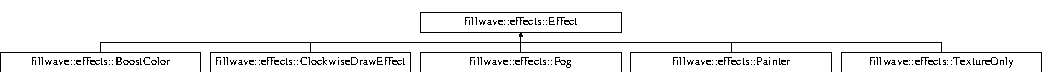
\includegraphics[height=0.961373cm]{classfillwave_1_1effects_1_1Effect}
\end{center}
\end{figure}
\subsection*{Public Member Functions}
\begin{DoxyCompactItemize}
\item 
virtual void \hyperlink{classfillwave_1_1effects_1_1Effect_a99c243cb10f504bfc6193e5e81926920}{pre\+Draw\+Action} (\hyperlink{classfillwave_1_1core_1_1Program}{core\+::\+Program} $\ast$program)=0
\begin{DoxyCompactList}\small\item\em virtual\+: defines action to be done just before the draw. \end{DoxyCompactList}\item 
virtual void \hyperlink{classfillwave_1_1effects_1_1Effect_ae01123633990402e11226c4d9a2dce1b}{post\+Draw\+Action} (\hyperlink{classfillwave_1_1core_1_1Program}{core\+::\+Program} $\ast$program)=0
\begin{DoxyCompactList}\small\item\em virtual\+: defines action to be done just after the draw. \end{DoxyCompactList}\item 
virtual void \hyperlink{classfillwave_1_1effects_1_1Effect_aed8c053b5798cbbc6668117989d18ead}{stop\+Action} (\hyperlink{classfillwave_1_1core_1_1Program}{core\+::\+Program} $\ast$program)=0
\begin{DoxyCompactList}\small\item\em virtual\+: defines action to be done when the effect is stopped. \end{DoxyCompactList}\item 
virtual void \hyperlink{classfillwave_1_1effects_1_1Effect_af0a4aa202fa7201cd19cedf71f6c682a}{start\+Action} (\hyperlink{classfillwave_1_1core_1_1Program}{core\+::\+Program} $\ast$program)=0
\begin{DoxyCompactList}\small\item\em virtual\+: defines action to be done when the effect is started. \end{DoxyCompactList}\end{DoxyCompactItemize}


\subsection{Detailed Description}
Base for effects. 

\subsection{Member Function Documentation}
\hypertarget{classfillwave_1_1effects_1_1Effect_ae01123633990402e11226c4d9a2dce1b}{}\index{fillwave\+::effects\+::\+Effect@{fillwave\+::effects\+::\+Effect}!post\+Draw\+Action@{post\+Draw\+Action}}
\index{post\+Draw\+Action@{post\+Draw\+Action}!fillwave\+::effects\+::\+Effect@{fillwave\+::effects\+::\+Effect}}
\subsubsection[{post\+Draw\+Action}]{\setlength{\rightskip}{0pt plus 5cm}virtual void fillwave\+::effects\+::\+Effect\+::post\+Draw\+Action (
\begin{DoxyParamCaption}
\item[{{\bf core\+::\+Program} $\ast$}]{program}
\end{DoxyParamCaption}
)\hspace{0.3cm}{\ttfamily [pure virtual]}}\label{classfillwave_1_1effects_1_1Effect_ae01123633990402e11226c4d9a2dce1b}


virtual\+: defines action to be done just after the draw. 

post\+Draw\+Action 

Implemented in \hyperlink{classfillwave_1_1effects_1_1Fog_a2a625835d139fb614a5325acba7604fc}{fillwave\+::effects\+::\+Fog}, \hyperlink{classfillwave_1_1effects_1_1Painter_a90b22772f264da46b7a2905b25025161}{fillwave\+::effects\+::\+Painter}, \hyperlink{classfillwave_1_1effects_1_1ClockwiseDrawEffect_a1565a96fe8744c414bfb0a082adce1d3}{fillwave\+::effects\+::\+Clockwise\+Draw\+Effect}, \hyperlink{classfillwave_1_1effects_1_1BoostColor_aeee3b3de532b1ea6aaac80590aa7f081}{fillwave\+::effects\+::\+Boost\+Color}, and \hyperlink{classfillwave_1_1effects_1_1TextureOnly_aaae24ae213873540c8fa55721d8e959f}{fillwave\+::effects\+::\+Texture\+Only}.

\hypertarget{classfillwave_1_1effects_1_1Effect_a99c243cb10f504bfc6193e5e81926920}{}\index{fillwave\+::effects\+::\+Effect@{fillwave\+::effects\+::\+Effect}!pre\+Draw\+Action@{pre\+Draw\+Action}}
\index{pre\+Draw\+Action@{pre\+Draw\+Action}!fillwave\+::effects\+::\+Effect@{fillwave\+::effects\+::\+Effect}}
\subsubsection[{pre\+Draw\+Action}]{\setlength{\rightskip}{0pt plus 5cm}virtual void fillwave\+::effects\+::\+Effect\+::pre\+Draw\+Action (
\begin{DoxyParamCaption}
\item[{{\bf core\+::\+Program} $\ast$}]{program}
\end{DoxyParamCaption}
)\hspace{0.3cm}{\ttfamily [pure virtual]}}\label{classfillwave_1_1effects_1_1Effect_a99c243cb10f504bfc6193e5e81926920}


virtual\+: defines action to be done just before the draw. 

pre\+Draw\+Action 

Implemented in \hyperlink{classfillwave_1_1effects_1_1Fog_a943f060680f000663eba8b2c93398ee8}{fillwave\+::effects\+::\+Fog}, \hyperlink{classfillwave_1_1effects_1_1Painter_a20bc2a09533498222c132e799c2c6080}{fillwave\+::effects\+::\+Painter}, \hyperlink{classfillwave_1_1effects_1_1ClockwiseDrawEffect_a0aa6fa5faf4d87d9defc4039f17fe615}{fillwave\+::effects\+::\+Clockwise\+Draw\+Effect}, \hyperlink{classfillwave_1_1effects_1_1BoostColor_ae5cbdf0c8487e4ee9743f39f9a6bf247}{fillwave\+::effects\+::\+Boost\+Color}, and \hyperlink{classfillwave_1_1effects_1_1TextureOnly_ada908a0505ac43646a6d2534f6189a66}{fillwave\+::effects\+::\+Texture\+Only}.

\hypertarget{classfillwave_1_1effects_1_1Effect_af0a4aa202fa7201cd19cedf71f6c682a}{}\index{fillwave\+::effects\+::\+Effect@{fillwave\+::effects\+::\+Effect}!start\+Action@{start\+Action}}
\index{start\+Action@{start\+Action}!fillwave\+::effects\+::\+Effect@{fillwave\+::effects\+::\+Effect}}
\subsubsection[{start\+Action}]{\setlength{\rightskip}{0pt plus 5cm}virtual void fillwave\+::effects\+::\+Effect\+::start\+Action (
\begin{DoxyParamCaption}
\item[{{\bf core\+::\+Program} $\ast$}]{program}
\end{DoxyParamCaption}
)\hspace{0.3cm}{\ttfamily [pure virtual]}}\label{classfillwave_1_1effects_1_1Effect_af0a4aa202fa7201cd19cedf71f6c682a}


virtual\+: defines action to be done when the effect is started. 

start\+Action 

Implemented in \hyperlink{classfillwave_1_1effects_1_1Fog_a8a7c4a0fb2f5cb95873d2b827354a4f8}{fillwave\+::effects\+::\+Fog}, \hyperlink{classfillwave_1_1effects_1_1Painter_a100a3bbf344ba7fef60ad9bbcb5fb93c}{fillwave\+::effects\+::\+Painter}, \hyperlink{classfillwave_1_1effects_1_1ClockwiseDrawEffect_a793f6c4d14c18bc366a17892d7764da8}{fillwave\+::effects\+::\+Clockwise\+Draw\+Effect}, \hyperlink{classfillwave_1_1effects_1_1BoostColor_aad6fdc26934cbdcd0cec735c987e653e}{fillwave\+::effects\+::\+Boost\+Color}, and \hyperlink{classfillwave_1_1effects_1_1TextureOnly_ac81c1c8d8e91fb53bc21ab90fad8f4a7}{fillwave\+::effects\+::\+Texture\+Only}.

\hypertarget{classfillwave_1_1effects_1_1Effect_aed8c053b5798cbbc6668117989d18ead}{}\index{fillwave\+::effects\+::\+Effect@{fillwave\+::effects\+::\+Effect}!stop\+Action@{stop\+Action}}
\index{stop\+Action@{stop\+Action}!fillwave\+::effects\+::\+Effect@{fillwave\+::effects\+::\+Effect}}
\subsubsection[{stop\+Action}]{\setlength{\rightskip}{0pt plus 5cm}virtual void fillwave\+::effects\+::\+Effect\+::stop\+Action (
\begin{DoxyParamCaption}
\item[{{\bf core\+::\+Program} $\ast$}]{program}
\end{DoxyParamCaption}
)\hspace{0.3cm}{\ttfamily [pure virtual]}}\label{classfillwave_1_1effects_1_1Effect_aed8c053b5798cbbc6668117989d18ead}


virtual\+: defines action to be done when the effect is stopped. 

stop\+Action 

Implemented in \hyperlink{classfillwave_1_1effects_1_1Fog_a2b5eb2628c9db559446619db744ebed5}{fillwave\+::effects\+::\+Fog}, \hyperlink{classfillwave_1_1effects_1_1Painter_a3180272825b161c45a5090e0b40f2797}{fillwave\+::effects\+::\+Painter}, \hyperlink{classfillwave_1_1effects_1_1ClockwiseDrawEffect_af496a94f611f378e365f0f56130201a9}{fillwave\+::effects\+::\+Clockwise\+Draw\+Effect}, \hyperlink{classfillwave_1_1effects_1_1BoostColor_a25ebaad4e773c6a4a147744655955a59}{fillwave\+::effects\+::\+Boost\+Color}, and \hyperlink{classfillwave_1_1effects_1_1TextureOnly_a4875d2b3f3c00db020583648d93578ce}{fillwave\+::effects\+::\+Texture\+Only}.



The documentation for this class was generated from the following file\+:\begin{DoxyCompactItemize}
\item 
/home/filip/\+Projects/fillwave/inc/fillwave/effects/Effect.\+h\end{DoxyCompactItemize}

\hypertarget{classfillwave_1_1particles_1_1EmiterPoint}{}\section{fillwave\+:\+:particles\+:\+:Emiter\+Point Class Reference}
\label{classfillwave_1_1particles_1_1EmiterPoint}\index{fillwave\+::particles\+::\+Emiter\+Point@{fillwave\+::particles\+::\+Emiter\+Point}}


Drawable Entity which emits particles.  




{\ttfamily \#include $<$Emiter\+Point.\+h$>$}

Inheritance diagram for fillwave\+:\+:particles\+:\+:Emiter\+Point\+:\begin{figure}[H]
\begin{center}
\leavevmode
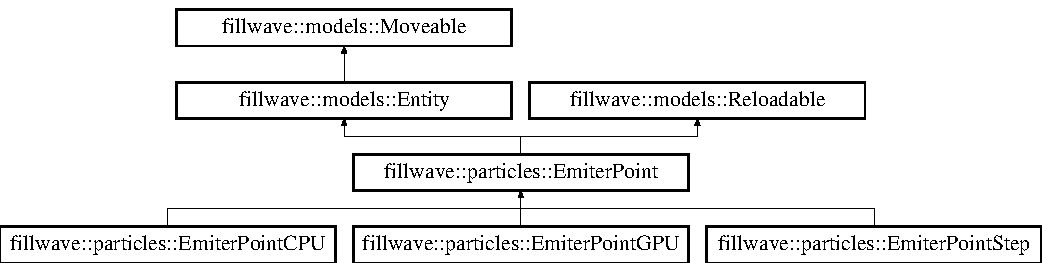
\includegraphics[height=3.538705cm]{classfillwave_1_1particles_1_1EmiterPoint}
\end{center}
\end{figure}
\subsection*{Public Member Functions}
\begin{DoxyCompactItemize}
\item 
\hypertarget{classfillwave_1_1particles_1_1EmiterPoint_a3245b754ca3c5b864a19b34a51054f95}{}{\bfseries Emiter\+Point} (\hyperlink{classfillwave_1_1Engine}{Engine} $\ast$engine, G\+Luint how\+Many, G\+Lfloat size, G\+Lfloat lifetime, p\+Texture texture, glm\+::vec4 color, G\+Lenum blending\+Source, G\+Lenum blending\+Destination, G\+Lboolean depth\+Testing, G\+Lfloat alpha\+Cut\+Off)\label{classfillwave_1_1particles_1_1EmiterPoint_a3245b754ca3c5b864a19b34a51054f95}

\item 
\hypertarget{classfillwave_1_1particles_1_1EmiterPoint_ade20253c3f719afd120aa99e0c74bf3c}{}virtual void {\bfseries update} (G\+Lfloat time\+Elapsed\+Sec)=0\label{classfillwave_1_1particles_1_1EmiterPoint_ade20253c3f719afd120aa99e0c74bf3c}

\item 
\hypertarget{classfillwave_1_1particles_1_1EmiterPoint_ae343ec1bb9f0c4fe4899f6750d4d3bd1}{}virtual void {\bfseries draw} (\hyperlink{classfillwave_1_1space_1_1Camera}{space\+::\+Camera} \&camera)=0\label{classfillwave_1_1particles_1_1EmiterPoint_ae343ec1bb9f0c4fe4899f6750d4d3bd1}

\item 
\hypertarget{classfillwave_1_1particles_1_1EmiterPoint_aeb90fa18eb1ace73adf28c449a769425}{}void {\bfseries set\+Blending\+Function} (G\+Lenum source\+Factor, G\+Lenum destination\+Factor)\label{classfillwave_1_1particles_1_1EmiterPoint_aeb90fa18eb1ace73adf28c449a769425}

\end{DoxyCompactItemize}
\subsection*{Protected Attributes}
\begin{DoxyCompactItemize}
\item 
\hypertarget{classfillwave_1_1particles_1_1EmiterPoint_a432862a8b60b237cf666034b7f4e6631}{}G\+Lfloat {\bfseries m\+Lifetime}\label{classfillwave_1_1particles_1_1EmiterPoint_a432862a8b60b237cf666034b7f4e6631}

\item 
\hypertarget{classfillwave_1_1particles_1_1EmiterPoint_a7b21efba8725dec2077cbe24a0326787}{}G\+Lfloat {\bfseries m\+Start\+Size}\label{classfillwave_1_1particles_1_1EmiterPoint_a7b21efba8725dec2077cbe24a0326787}

\item 
\hypertarget{classfillwave_1_1particles_1_1EmiterPoint_aa5c5cfa16a8572abdfcdc7ef43584926}{}G\+Lfloat {\bfseries m\+How\+Many}\label{classfillwave_1_1particles_1_1EmiterPoint_aa5c5cfa16a8572abdfcdc7ef43584926}

\item 
\hypertarget{classfillwave_1_1particles_1_1EmiterPoint_a2aae19d04e6fc4588df04deb0bdf375e}{}G\+Lboolean {\bfseries m\+Depth\+Testing}\label{classfillwave_1_1particles_1_1EmiterPoint_a2aae19d04e6fc4588df04deb0bdf375e}

\item 
\hypertarget{classfillwave_1_1particles_1_1EmiterPoint_a791d44885d90f128b1dea14c791c8210}{}glm\+::vec4 {\bfseries m\+Color}\label{classfillwave_1_1particles_1_1EmiterPoint_a791d44885d90f128b1dea14c791c8210}

\item 
\hypertarget{classfillwave_1_1particles_1_1EmiterPoint_aa31cbe23578f5c3dd18d3c1c022eb9d0}{}\hyperlink{structfillwave_1_1common_1_1Blending}{common\+::\+Blending} {\bfseries m\+Blending}\label{classfillwave_1_1particles_1_1EmiterPoint_aa31cbe23578f5c3dd18d3c1c022eb9d0}

\item 
\hypertarget{classfillwave_1_1particles_1_1EmiterPoint_ab25fae6bfb786e0e968940f3ad609c50}{}G\+Lfloat {\bfseries m\+Alpha\+Cut\+Off}\label{classfillwave_1_1particles_1_1EmiterPoint_ab25fae6bfb786e0e968940f3ad609c50}

\item 
\hypertarget{classfillwave_1_1particles_1_1EmiterPoint_a1820e714db6b0fc13175d6970870a9c9}{}p\+Program {\bfseries m\+Program}\label{classfillwave_1_1particles_1_1EmiterPoint_a1820e714db6b0fc13175d6970870a9c9}

\item 
\hypertarget{classfillwave_1_1particles_1_1EmiterPoint_ae07905d07f70c71c172bd1339fc5b792}{}p\+Index\+Buffer\+Particles {\bfseries m\+I\+B\+O}\label{classfillwave_1_1particles_1_1EmiterPoint_ae07905d07f70c71c172bd1339fc5b792}

\item 
\hypertarget{classfillwave_1_1particles_1_1EmiterPoint_a8f1d516b9bc56d37f9c9acb422ea2a16}{}p\+Texture {\bfseries m\+Texture}\label{classfillwave_1_1particles_1_1EmiterPoint_a8f1d516b9bc56d37f9c9acb422ea2a16}

\end{DoxyCompactItemize}


\subsection{Detailed Description}
Drawable Entity which emits particles. 

The documentation for this class was generated from the following file\+:\begin{DoxyCompactItemize}
\item 
/home/filip/\+Projects/fillwave/inc/fillwave/particles/Emiter\+Point.\+h\end{DoxyCompactItemize}

\hypertarget{classfillwave_1_1particles_1_1EmiterPointCPU}{}\section{fillwave\+:\+:particles\+:\+:Emiter\+Point\+C\+P\+U Class Reference}
\label{classfillwave_1_1particles_1_1EmiterPointCPU}\index{fillwave\+::particles\+::\+Emiter\+Point\+C\+P\+U@{fillwave\+::particles\+::\+Emiter\+Point\+C\+P\+U}}


Polynomial particle Emiter. Can generate a particles with velocity, direction, and acceleration defined by the user.  




{\ttfamily \#include $<$Emiter\+Point\+C\+P\+U.\+h$>$}

Inheritance diagram for fillwave\+:\+:particles\+:\+:Emiter\+Point\+C\+P\+U\+:\begin{figure}[H]
\begin{center}
\leavevmode
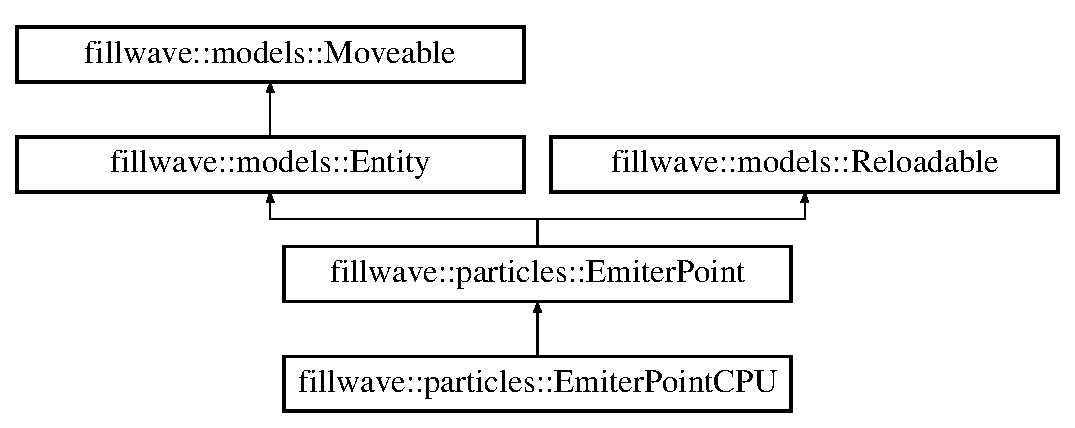
\includegraphics[height=4.000000cm]{classfillwave_1_1particles_1_1EmiterPointCPU}
\end{center}
\end{figure}
\subsection*{Public Member Functions}
\begin{DoxyCompactItemize}
\item 
\hypertarget{classfillwave_1_1particles_1_1EmiterPointCPU_a6aab1f8b79a2644cfc41b1c9b8c20a2e}{}{\bfseries Emiter\+Point\+C\+P\+U} (\hyperlink{classfillwave_1_1Engine}{Engine} $\ast$engine, G\+Lfloat emiting\+Source\+Rate, G\+Luint how\+Many, glm\+::vec4 color, glm\+::vec3 acceleration=glm\+::vec3(0.\+0), glm\+::vec3 start\+Velocity=glm\+::vec3(0.\+0), glm\+::vec3 robustness\+Velocity=glm\+::vec3(0.\+0), glm\+::vec3 start\+Position=glm\+::vec3(0.\+0), glm\+::vec3 robustness\+Position=glm\+::vec3(0.\+0), G\+Lfloat start\+Size=1.\+0, G\+Lfloat lifetime=6.\+0, p\+Texture texture=p\+Texture(), G\+Lenum blending\+Source=G\+L\+\_\+\+S\+R\+C\+\_\+\+A\+L\+P\+H\+A, G\+Lenum blending\+Destination=G\+L\+\_\+\+O\+N\+E\+\_\+\+M\+I\+N\+U\+S\+\_\+\+S\+R\+C\+\_\+\+A\+L\+P\+H\+A, G\+Lboolean depth\+Testing=G\+L\+\_\+\+T\+R\+U\+E, G\+Lfloat alpha\+Cut\+Off\+Level=0.\+0)\label{classfillwave_1_1particles_1_1EmiterPointCPU_a6aab1f8b79a2644cfc41b1c9b8c20a2e}

\item 
\hypertarget{classfillwave_1_1particles_1_1EmiterPointCPU_a7f3440a25739cee2c3524f18f4b97e9c}{}void {\bfseries update} (G\+Lfloat time\+Elapsed\+Sec)\label{classfillwave_1_1particles_1_1EmiterPointCPU_a7f3440a25739cee2c3524f18f4b97e9c}

\item 
\hypertarget{classfillwave_1_1particles_1_1EmiterPointCPU_ad752356f2a1e1ae49a273c9eba049edf}{}void {\bfseries draw} (\hyperlink{classfillwave_1_1space_1_1Camera}{space\+::\+Camera} \&camera)\label{classfillwave_1_1particles_1_1EmiterPointCPU_ad752356f2a1e1ae49a273c9eba049edf}

\end{DoxyCompactItemize}
\subsection*{Additional Inherited Members}


\subsection{Detailed Description}
Polynomial particle Emiter. Can generate a particles with velocity, direction, and acceleration defined by the user. 

The documentation for this class was generated from the following file\+:\begin{DoxyCompactItemize}
\item 
/home/filip/\+Projects/fillwave/inc/fillwave/particles/Emiter\+Point\+C\+P\+U.\+h\end{DoxyCompactItemize}

\hypertarget{classfillwave_1_1particles_1_1EmiterPointGPU}{}\section{fillwave\+:\+:particles\+:\+:Emiter\+Point\+G\+P\+U Class Reference}
\label{classfillwave_1_1particles_1_1EmiterPointGPU}\index{fillwave\+::particles\+::\+Emiter\+Point\+G\+P\+U@{fillwave\+::particles\+::\+Emiter\+Point\+G\+P\+U}}


Polynomial particle Emiter entirely computed on G\+P\+U. Can generate a particles with velocity, direction, and acceleration defined by the user.  




{\ttfamily \#include $<$Emiter\+Point\+G\+P\+U.\+h$>$}

Inheritance diagram for fillwave\+:\+:particles\+:\+:Emiter\+Point\+G\+P\+U\+:\begin{figure}[H]
\begin{center}
\leavevmode
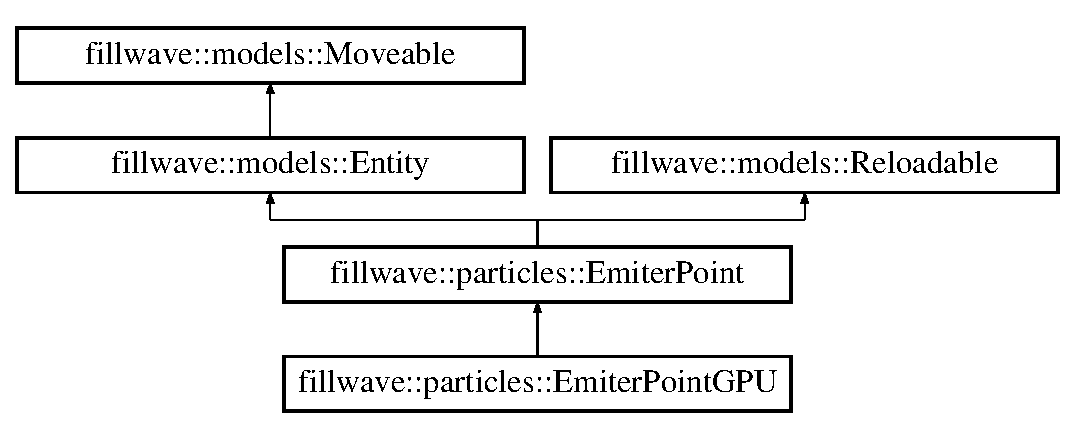
\includegraphics[height=4.000000cm]{classfillwave_1_1particles_1_1EmiterPointGPU}
\end{center}
\end{figure}
\subsection*{Public Member Functions}
\begin{DoxyCompactItemize}
\item 
\hypertarget{classfillwave_1_1particles_1_1EmiterPointGPU_a2919404fb0957db6954f201e4b24df02}{}{\bfseries Emiter\+Point\+G\+P\+U} (\hyperlink{classfillwave_1_1Engine}{Engine} $\ast$engine, G\+Lfloat emiting\+Source\+Rate, G\+Luint how\+Many, glm\+::vec4 color, glm\+::vec3 acceleration, glm\+::vec3 start\+Velocity, glm\+::vec3 robustness\+Velocity, glm\+::vec3 start\+Position, glm\+::vec3 robustness\+Position, G\+Lfloat start\+Size, G\+Lfloat lifetime, p\+Texture texture, G\+Lenum blending\+Source, G\+Lenum blending\+Destination, G\+Lboolean depth\+Testing, G\+Lfloat alpha\+Cut\+Off\+Level=0.\+0)\label{classfillwave_1_1particles_1_1EmiterPointGPU_a2919404fb0957db6954f201e4b24df02}

\item 
\hypertarget{classfillwave_1_1particles_1_1EmiterPointGPU_a2188ac7f0ad767c46c9a72576041c5a1}{}void {\bfseries draw} (\hyperlink{classfillwave_1_1space_1_1Camera}{space\+::\+Camera} \&camera)\label{classfillwave_1_1particles_1_1EmiterPointGPU_a2188ac7f0ad767c46c9a72576041c5a1}

\item 
\hypertarget{classfillwave_1_1particles_1_1EmiterPointGPU_ab5b0ef9c79b0210be09a7dd1825a7423}{}void {\bfseries update} (G\+Lfloat time\+Elapsed\+Sec)\label{classfillwave_1_1particles_1_1EmiterPointGPU_ab5b0ef9c79b0210be09a7dd1825a7423}

\end{DoxyCompactItemize}
\subsection*{Additional Inherited Members}


\subsection{Detailed Description}
Polynomial particle Emiter entirely computed on G\+P\+U. Can generate a particles with velocity, direction, and acceleration defined by the user. 

The documentation for this class was generated from the following file\+:\begin{DoxyCompactItemize}
\item 
/home/filip/\+Projects/fillwave/inc/fillwave/particles/Emiter\+Point\+G\+P\+U.\+h\end{DoxyCompactItemize}

\hypertarget{classfillwave_1_1particles_1_1EmiterPointStep}{}\section{fillwave\+:\+:particles\+:\+:Emiter\+Point\+Step Class Reference}
\label{classfillwave_1_1particles_1_1EmiterPointStep}\index{fillwave\+::particles\+::\+Emiter\+Point\+Step@{fillwave\+::particles\+::\+Emiter\+Point\+Step}}


Not used.  




{\ttfamily \#include $<$Emiter\+Point\+Step.\+h$>$}

Inheritance diagram for fillwave\+:\+:particles\+:\+:Emiter\+Point\+Step\+:\begin{figure}[H]
\begin{center}
\leavevmode
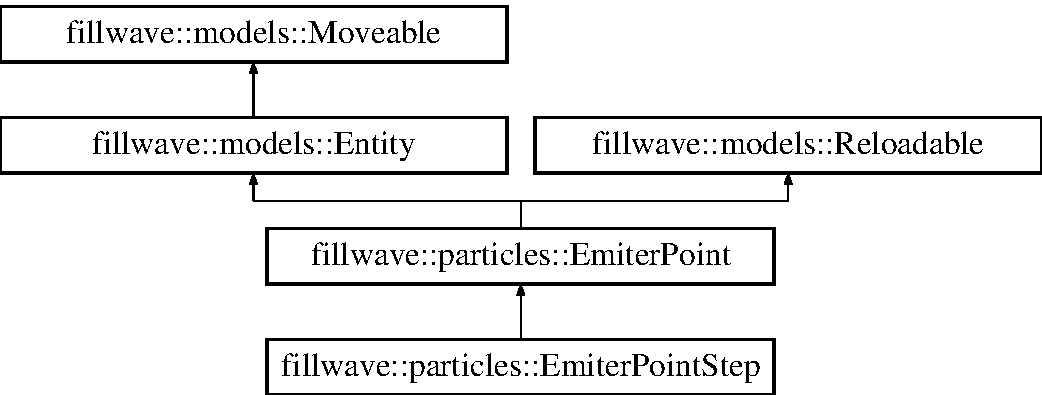
\includegraphics[height=4.000000cm]{classfillwave_1_1particles_1_1EmiterPointStep}
\end{center}
\end{figure}
\subsection*{Public Member Functions}
\begin{DoxyCompactItemize}
\item 
\hypertarget{classfillwave_1_1particles_1_1EmiterPointStep_abfc1d17e500f5849ec9b4949e7bd5f54}{}{\bfseries Emiter\+Point\+Step} (\hyperlink{classfillwave_1_1Engine}{Engine} $\ast$engine, G\+Lint how\+Many, G\+Lenum blending\+Source, G\+Lenum blending\+Destination, p\+Texture texture)\label{classfillwave_1_1particles_1_1EmiterPointStep_abfc1d17e500f5849ec9b4949e7bd5f54}

\end{DoxyCompactItemize}
\subsection*{Additional Inherited Members}


\subsection{Detailed Description}
Not used. 

The documentation for this class was generated from the following file\+:\begin{DoxyCompactItemize}
\item 
/home/filip/\+Projects/fillwave/inc/fillwave/particles/Emiter\+Point\+Step.\+h\end{DoxyCompactItemize}

\hypertarget{classfillwave_1_1Engine}{}\section{fillwave\+:\+:Engine Class Reference}
\label{classfillwave_1_1Engine}\index{fillwave\+::\+Engine@{fillwave\+::\+Engine}}


Fillwave engine.  




{\ttfamily \#include $<$Fillwave.\+h$>$}

\subsection*{Classes}
\begin{DoxyCompactItemize}
\item 
struct \hyperlink{structfillwave_1_1Engine_1_1EngineImpl}{Engine\+Impl}
\end{DoxyCompactItemize}
\subsection*{Public Member Functions}
\begin{DoxyCompactItemize}
\item 
\hypertarget{classfillwave_1_1Engine_a6348c216dda393c0ec969a1871f286b0}{}{\bfseries Engine} (G\+Lint argc, G\+Lchar $\ast$const argv\mbox{[}$\,$\mbox{]})\label{classfillwave_1_1Engine_a6348c216dda393c0ec969a1871f286b0}

\item 
\hypertarget{classfillwave_1_1Engine_a8ab70999c6424f4aff5eea39a23793fb}{}void {\bfseries configure\+Debugger} (e\+Debugger\+State state)\label{classfillwave_1_1Engine_a8ab70999c6424f4aff5eea39a23793fb}

\item 
\hypertarget{classfillwave_1_1Engine_a79b8431174a0e21ee33550bb17435572}{}void {\bfseries configure\+File\+Logging} (std\+::string file\+Name=\char`\"{}\char`\"{})\label{classfillwave_1_1Engine_a79b8431174a0e21ee33550bb17435572}

\item 
\hypertarget{classfillwave_1_1Engine_afeda6ab5368be17d98e6c1a703968ddd}{}void {\bfseries configure\+F\+P\+S\+Counter} (std\+::string font\+Name=\char`\"{}\char`\"{}, G\+Lfloat x\+Position=-\/0.\+95, G\+Lfloat y\+Position=0.\+95, G\+Lfloat size=100.\+0)\label{classfillwave_1_1Engine_afeda6ab5368be17d98e6c1a703968ddd}

\item 
\hypertarget{classfillwave_1_1Engine_a317929adad6bac338fe9de406256aafc}{}void {\bfseries configure\+Background\+Color} (glm\+::vec3 color)\label{classfillwave_1_1Engine_a317929adad6bac338fe9de406256aafc}

\item 
\hypertarget{classfillwave_1_1Engine_afca8e958d13dc33cbe336db17bd2f1c7}{}void {\bfseries configure\+Time} (G\+Lfloat time\+Factor)\label{classfillwave_1_1Engine_afca8e958d13dc33cbe336db17bd2f1c7}

\item 
\hypertarget{classfillwave_1_1Engine_ae6b333344d6322eb369f6d53fe24d292}{}void {\bfseries draw} (G\+Lfloat time)\label{classfillwave_1_1Engine_ae6b333344d6322eb369f6d53fe24d292}

\item 
\hypertarget{classfillwave_1_1Engine_af9320dfea90a32c439e67ddb08262b15}{}void {\bfseries draw\+Lines} (G\+Lfloat time)\label{classfillwave_1_1Engine_af9320dfea90a32c439e67ddb08262b15}

\item 
\hypertarget{classfillwave_1_1Engine_a29d9953bd25b6cd33b9bf1f0ea5df431}{}void {\bfseries draw\+Points} (G\+Lfloat time)\label{classfillwave_1_1Engine_a29d9953bd25b6cd33b9bf1f0ea5df431}

\item 
\hypertarget{classfillwave_1_1Engine_a459fceda9f89ab99df831fb3dcef6f55}{}void {\bfseries draw\+Texture} (\hyperlink{classfillwave_1_1core_1_1Texture}{core\+::\+Texture} $\ast$t, \hyperlink{classfillwave_1_1core_1_1Program}{core\+::\+Program} $\ast$p)\label{classfillwave_1_1Engine_a459fceda9f89ab99df831fb3dcef6f55}

\item 
\hypertarget{classfillwave_1_1Engine_a5755d2d20fd2a24c95282adc6263cbbe}{}void {\bfseries draw\+Texture} (\hyperlink{classfillwave_1_1core_1_1Texture}{core\+::\+Texture} $\ast$t)\label{classfillwave_1_1Engine_a5755d2d20fd2a24c95282adc6263cbbe}

\item 
\hypertarget{classfillwave_1_1Engine_a16884ac1bd9a55ee11cb915bc7ac1bad}{}pu\+Physics\+Mesh\+Buffer {\bfseries get\+Physical\+Mesh\+Buffer} (const std\+::string \&shape\+Path)\label{classfillwave_1_1Engine_a16884ac1bd9a55ee11cb915bc7ac1bad}

\item 
\hypertarget{classfillwave_1_1Engine_aee372063724f3029b0f41ec4b826106e}{}\hyperlink{classfillwave_1_1manager_1_1LightManager}{manager\+::\+Light\+Manager} $\ast$ {\bfseries get\+Light\+Manager} () const \label{classfillwave_1_1Engine_aee372063724f3029b0f41ec4b826106e}

\item 
\hypertarget{classfillwave_1_1Engine_a29a0fe99323dc6150ad3cddfb49e752f}{}const f\+Scene $\ast$ {\bfseries get\+Model\+From\+File} (std\+::string path)\label{classfillwave_1_1Engine_a29a0fe99323dc6150ad3cddfb49e752f}

\item 
\hypertarget{classfillwave_1_1Engine_aa7001ee49ec51a6a47fdd3b9fa0619df}{}void {\bfseries set\+Current\+Scene} (p\+Scene scene)\label{classfillwave_1_1Engine_aa7001ee49ec51a6a47fdd3b9fa0619df}

\item 
\hypertarget{classfillwave_1_1Engine_aa8f9cf557a945bec3447af175888b256}{}p\+Scene {\bfseries get\+Current\+Scene} () const \label{classfillwave_1_1Engine_aa8f9cf557a945bec3447af175888b256}

\item 
\hypertarget{classfillwave_1_1Engine_a019edbfa9aa9dcae5775e909df489248}{}G\+Luint {\bfseries get\+Frames\+Passed} ()\label{classfillwave_1_1Engine_a019edbfa9aa9dcae5775e909df489248}

\item 
\hypertarget{classfillwave_1_1Engine_acb3c6c716c79148844d95de53dd76977}{}G\+Lfloat {\bfseries get\+Startup\+Animation\+Time} () const \label{classfillwave_1_1Engine_acb3c6c716c79148844d95de53dd76977}

\item 
\hypertarget{classfillwave_1_1Engine_a5ba05b3ad8f87b5a91dffe0abfefc586}{}p\+Shader {\bfseries store\+Shader\+Fragment} (const std\+::string \&shader\+Path)\label{classfillwave_1_1Engine_a5ba05b3ad8f87b5a91dffe0abfefc586}

\item 
\hypertarget{classfillwave_1_1Engine_a993e9b3f716bb832d017df28b76e949c}{}p\+Shader {\bfseries store\+Shader\+Vertex} (const std\+::string \&shader\+Path)\label{classfillwave_1_1Engine_a993e9b3f716bb832d017df28b76e949c}

\item 
\hypertarget{classfillwave_1_1Engine_a198587bb1ba07669dc9662f2a77ef23a}{}p\+Shader {\bfseries store\+Shader\+Fragment} (const std\+::string \&shader\+Path, const std\+::string \&shader\+Source)\label{classfillwave_1_1Engine_a198587bb1ba07669dc9662f2a77ef23a}

\item 
\hypertarget{classfillwave_1_1Engine_a63be33b71b6541023cc986e12a20835a}{}p\+Shader {\bfseries store\+Shader\+Vertex} (const std\+::string \&shader\+Path, const std\+::string \&shader\+Source)\label{classfillwave_1_1Engine_a63be33b71b6541023cc986e12a20835a}

\item 
\hypertarget{classfillwave_1_1Engine_a0597b16a02320880925f66a85dddd154}{}p\+Shader {\bfseries store\+Shader\+Geometry} (const std\+::string \&shader\+Path)\label{classfillwave_1_1Engine_a0597b16a02320880925f66a85dddd154}

\item 
\hypertarget{classfillwave_1_1Engine_a7157ddacfcb0dc57f905dd55c5e8298c}{}p\+Shader {\bfseries store\+Shader\+Tesselation\+Control} (const std\+::string \&shader\+Path)\label{classfillwave_1_1Engine_a7157ddacfcb0dc57f905dd55c5e8298c}

\item 
\hypertarget{classfillwave_1_1Engine_a92e54f7f0ff3fb02d39fcff1e24508fc}{}p\+Shader {\bfseries store\+Shader\+Tesselation\+Evaluation} (const std\+::string \&shader\+Path)\label{classfillwave_1_1Engine_a92e54f7f0ff3fb02d39fcff1e24508fc}

\item 
\hypertarget{classfillwave_1_1Engine_a0397857b8de836c68499c88612756e61}{}p\+Shader {\bfseries store\+Shader\+Geometry} (const std\+::string \&shader\+Path, const std\+::string \&shader\+Source)\label{classfillwave_1_1Engine_a0397857b8de836c68499c88612756e61}

\item 
\hypertarget{classfillwave_1_1Engine_ac076814ab5f44ce033fa0bc1cb8e0500}{}p\+Shader {\bfseries store\+Shader\+Tesselation\+Control} (const std\+::string \&shader\+Path, const std\+::string \&shader\+Source)\label{classfillwave_1_1Engine_ac076814ab5f44ce033fa0bc1cb8e0500}

\item 
\hypertarget{classfillwave_1_1Engine_af226a5bf69d8380adb04d3e53ee41689}{}p\+Shader {\bfseries store\+Shader\+Tesselation\+Evaluation} (const std\+::string \&shader\+Path, const std\+::string \&shader\+Source)\label{classfillwave_1_1Engine_af226a5bf69d8380adb04d3e53ee41689}

\item 
\hypertarget{classfillwave_1_1Engine_ad8cbc06ff1f9bba8e3cef59a3c876126}{}p\+Program {\bfseries store\+Program} (const std\+::string \&name, const std\+::vector$<$ p\+Shader $>$ \&shaders, G\+Lboolean skip\+Linking=G\+L\+\_\+\+F\+A\+L\+S\+E)\label{classfillwave_1_1Engine_ad8cbc06ff1f9bba8e3cef59a3c876126}

\item 
\hypertarget{classfillwave_1_1Engine_ad4bde7a3e530211b7aa9ed273e055ff9}{}p\+Texture {\bfseries store\+Texture} (const std\+::string \&texture\+Path, const G\+Luint \&map\+Type=F\+I\+L\+L\+W\+A\+V\+E\+\_\+\+T\+E\+X\+T\+U\+R\+E\+\_\+\+T\+Y\+P\+E\+\_\+\+N\+O\+N\+E, loader\+::e\+Compression compression=loader\+::e\+Compression\+::none)\label{classfillwave_1_1Engine_ad4bde7a3e530211b7aa9ed273e055ff9}

\item 
\hypertarget{classfillwave_1_1Engine_a8defb3db1fc8882f967c012a79afeff0}{}p\+Texture2\+D\+Renderable\+Dynamic {\bfseries store\+Texture\+Dynamic} (const std\+::string \&fragment\+Shader\+Path)\label{classfillwave_1_1Engine_a8defb3db1fc8882f967c012a79afeff0}

\item 
\hypertarget{classfillwave_1_1Engine_a3c3207e65c948a73ddb07021687c4a35}{}p\+Texture3\+D {\bfseries store\+Texture3\+D} (const std\+::string \&pos\+X, const std\+::string \&neg\+X, const std\+::string \&pos\+Y, const std\+::string \&neg\+Y, const std\+::string \&pos\+Z, const std\+::string \&neg\+Z)\label{classfillwave_1_1Engine_a3c3207e65c948a73ddb07021687c4a35}

\item 
\hypertarget{classfillwave_1_1Engine_acef6ad430f102bca3d6975c4a2c3f17a}{}p\+Light\+Spot {\bfseries store\+Light\+Spot} (glm\+::vec3 position, glm\+::quat rotation, glm\+::vec4 color, p\+Entity entity=p\+Entity())\label{classfillwave_1_1Engine_acef6ad430f102bca3d6975c4a2c3f17a}

\item 
\hypertarget{classfillwave_1_1Engine_a46cb84111218f318dbc2f1143f4ee277}{}p\+Light\+Point {\bfseries store\+Light\+Point} (glm\+::vec3 position, glm\+::vec4 color, p\+Entity entity=p\+Entity())\label{classfillwave_1_1Engine_a46cb84111218f318dbc2f1143f4ee277}

\item 
\hypertarget{classfillwave_1_1Engine_a3b70a285ba9d5e912d71e1ba504b2880}{}p\+Light\+Directional {\bfseries store\+Light\+Directional} (glm\+::vec3 position, glm\+::quat rotation, glm\+::vec4 color, p\+Entity entity=p\+Entity())\label{classfillwave_1_1Engine_a3b70a285ba9d5e912d71e1ba504b2880}

\item 
\hypertarget{classfillwave_1_1Engine_a96be4bcbb09810e004ca585fde819b68}{}p\+Text {\bfseries store\+Text} (std\+::string content, std\+::string font\+Name, G\+Lfloat starting\+Position\+X, G\+Lfloat starting\+Position\+Y, G\+Lfloat scale=1.\+0, glm\+::vec4 color=glm\+::vec4(1.\+0, 1.\+0, 1.\+0, 1.\+0), e\+Text\+Effect effect=e\+Text\+Effect\+::none)\label{classfillwave_1_1Engine_a96be4bcbb09810e004ca585fde819b68}

\item 
\hypertarget{classfillwave_1_1Engine_ae3619e901e208d1c61ebced3b18997e3}{}p\+Sampler {\bfseries store\+S\+O} (G\+Lint texture\+Unit)\label{classfillwave_1_1Engine_ae3619e901e208d1c61ebced3b18997e3}

\item 
\hypertarget{classfillwave_1_1Engine_a40bb53bfae5e06d4238f5a07c4f30a87}{}p\+Vertex\+Array {\bfseries store\+V\+A\+O} (\hyperlink{classfillwave_1_1models_1_1Reloadable}{models\+::\+Reloadable} $\ast$user=nullptr)\label{classfillwave_1_1Engine_a40bb53bfae5e06d4238f5a07c4f30a87}

\item 
\hypertarget{classfillwave_1_1Engine_a1f7390160abe6d9ef530b27ac8180017}{}void {\bfseries clear\+Text} (p\+Text text)\label{classfillwave_1_1Engine_a1f7390160abe6d9ef530b27ac8180017}

\item 
\hypertarget{classfillwave_1_1Engine_a487281fb62a0e3469759afb0ad0f4708}{}void {\bfseries clear\+Light} (p\+Light\+Spot light)\label{classfillwave_1_1Engine_a487281fb62a0e3469759afb0ad0f4708}

\item 
\hypertarget{classfillwave_1_1Engine_a68cf4c1c889f24ac5f7d39a26e3a0c7d}{}void {\bfseries clear\+Light} (p\+Light\+Directional)\label{classfillwave_1_1Engine_a68cf4c1c889f24ac5f7d39a26e3a0c7d}

\item 
\hypertarget{classfillwave_1_1Engine_a54d9508e54fc6e503701c52704027c82}{}void {\bfseries clear\+Light} (p\+Light\+Point light)\label{classfillwave_1_1Engine_a54d9508e54fc6e503701c52704027c82}

\item 
\hypertarget{classfillwave_1_1Engine_a6e6a32a9f0731403d647f76c73c954c1}{}void {\bfseries clear\+Lights} ()\label{classfillwave_1_1Engine_a6e6a32a9f0731403d647f76c73c954c1}

\item 
\hypertarget{classfillwave_1_1Engine_a6433c8aa182194e019b5a8003a541ad8}{}void {\bfseries pick} (G\+Luint x, G\+Luint y)\label{classfillwave_1_1Engine_a6433c8aa182194e019b5a8003a541ad8}

\item 
\hypertarget{classfillwave_1_1Engine_aa8a511f8d92f5109c50c6b1bac4ebdc4}{}glm\+::ivec2 {\bfseries get\+Screen\+Size} () const \label{classfillwave_1_1Engine_aa8a511f8d92f5109c50c6b1bac4ebdc4}

\item 
\hypertarget{classfillwave_1_1Engine_a622e9159a52582ac0fadd7be6ad2d31a}{}void {\bfseries log} ()\label{classfillwave_1_1Engine_a622e9159a52582ac0fadd7be6ad2d31a}

\item 
\hypertarget{classfillwave_1_1Engine_a4e08aacaa4023e9a2688ed4fd0b4bd31}{}void {\bfseries capture\+Framebuffer\+To\+File} (const std\+::string \&name)\label{classfillwave_1_1Engine_a4e08aacaa4023e9a2688ed4fd0b4bd31}

\item 
\hypertarget{classfillwave_1_1Engine_a0d0b79df4b9f1589c526cdb7fbc0a968}{}void {\bfseries capture\+Framebuffer\+To\+Buffer} (G\+Lubyte $\ast$buffer, G\+Lint $\ast$size\+In\+Bytes, G\+Luint format=G\+L\+\_\+\+R\+G\+B\+A, G\+Lint bytes\+Per\+Pixel=4)\label{classfillwave_1_1Engine_a0d0b79df4b9f1589c526cdb7fbc0a968}

\item 
\hypertarget{classfillwave_1_1Engine_a73dd41624a311f1242ccddc4584f0ae2}{}void {\bfseries add\+Post\+Process} (const std\+::string \&fragment\+Shader\+Path, G\+Lfloat life\+Time=F\+I\+L\+L\+W\+A\+V\+E\+\_\+\+E\+N\+D\+L\+E\+S\+S)\label{classfillwave_1_1Engine_a73dd41624a311f1242ccddc4584f0ae2}

\item 
\hypertarget{classfillwave_1_1Engine_a27e7826505b51d009d13ab433b70e00b}{}void {\bfseries set\+Focus\+Key} (p\+Entity entity)\label{classfillwave_1_1Engine_a27e7826505b51d009d13ab433b70e00b}

\item 
\hypertarget{classfillwave_1_1Engine_a49d11248e32d308e024a13cf3c12982f}{}void {\bfseries set\+Focus\+Mouse\+Button} (p\+Entity entity)\label{classfillwave_1_1Engine_a49d11248e32d308e024a13cf3c12982f}

\item 
\hypertarget{classfillwave_1_1Engine_a83e437788bfb4743ae3e334ce3d847d4}{}void {\bfseries set\+Focus\+Scroll} (p\+Entity entity)\label{classfillwave_1_1Engine_a83e437788bfb4743ae3e334ce3d847d4}

\item 
\hypertarget{classfillwave_1_1Engine_ad85af270ea7c6a4ee06ff263d02b0f87}{}void {\bfseries set\+Focus\+Char} (p\+Entity entity)\label{classfillwave_1_1Engine_ad85af270ea7c6a4ee06ff263d02b0f87}

\item 
\hypertarget{classfillwave_1_1Engine_a58cf1ec7c9b31011cb3200c797f2719e}{}void {\bfseries set\+Focus\+Char\+Mods} (p\+Entity entity)\label{classfillwave_1_1Engine_a58cf1ec7c9b31011cb3200c797f2719e}

\item 
\hypertarget{classfillwave_1_1Engine_a0c474a1ea1c0704638cfcfd62de72f5f}{}void {\bfseries set\+Focus\+Cursor\+Enter} (p\+Entity entity)\label{classfillwave_1_1Engine_a0c474a1ea1c0704638cfcfd62de72f5f}

\item 
\hypertarget{classfillwave_1_1Engine_a9b81fd9dea4b2d0cb16dcfe1c5ba2705}{}void {\bfseries set\+Focus\+Cursor\+Position} (p\+Entity entity)\label{classfillwave_1_1Engine_a9b81fd9dea4b2d0cb16dcfe1c5ba2705}

\item 
\hypertarget{classfillwave_1_1Engine_a6cdeeb61f95f2ea2c8d0748c44602a4f}{}p\+Entity {\bfseries get\+Focus\+Key} () const \label{classfillwave_1_1Engine_a6cdeeb61f95f2ea2c8d0748c44602a4f}

\item 
\hypertarget{classfillwave_1_1Engine_ab198e289259c69e826d61c3e58511ce1}{}p\+Entity {\bfseries get\+Focus\+Mouse\+Button} () const \label{classfillwave_1_1Engine_ab198e289259c69e826d61c3e58511ce1}

\item 
\hypertarget{classfillwave_1_1Engine_a971c8773f4fb5065cb4acca6bc6d586e}{}p\+Entity {\bfseries get\+Focus\+Scroll} () const \label{classfillwave_1_1Engine_a971c8773f4fb5065cb4acca6bc6d586e}

\item 
\hypertarget{classfillwave_1_1Engine_a02a4a3c0e5d46bdabfdb7dc6887143cb}{}p\+Entity {\bfseries get\+Focus\+Char} () const \label{classfillwave_1_1Engine_a02a4a3c0e5d46bdabfdb7dc6887143cb}

\item 
\hypertarget{classfillwave_1_1Engine_a328004b38586dbd571230b666098e701}{}p\+Entity {\bfseries get\+Focus\+Char\+Mods} () const \label{classfillwave_1_1Engine_a328004b38586dbd571230b666098e701}

\item 
\hypertarget{classfillwave_1_1Engine_a42fb9efb98c8c4be2cca3de94bd86a3e}{}p\+Entity {\bfseries get\+Focus\+Cursor\+Enter} () const \label{classfillwave_1_1Engine_a42fb9efb98c8c4be2cca3de94bd86a3e}

\item 
\hypertarget{classfillwave_1_1Engine_adb0369bdcbfe6e6dad399c1978f86d87}{}p\+Entity {\bfseries get\+Focus\+Cursor\+Position} () const \label{classfillwave_1_1Engine_adb0369bdcbfe6e6dad399c1978f86d87}

\item 
\hypertarget{classfillwave_1_1Engine_a333f8f38b26b8b7720b720fc9cedf24e}{}p\+Entity {\bfseries get\+Focus\+Touch\+Screen} () const \label{classfillwave_1_1Engine_a333f8f38b26b8b7720b720fc9cedf24e}

\item 
\hypertarget{classfillwave_1_1Engine_ab5a508e59472b0653897b4c69ec09a63}{}void {\bfseries insert\+Resize\+Screen} (G\+Luint width, G\+Luint height)\label{classfillwave_1_1Engine_ab5a508e59472b0653897b4c69ec09a63}

\item 
\hypertarget{classfillwave_1_1Engine_aa5e13d284305180bf20d10305d8872b5}{}void {\bfseries insert\+Input\+Key} (\hyperlink{classfillwave_1_1actions_1_1KeyboardEvent}{actions\+::\+Keyboard\+Event} \&event)\label{classfillwave_1_1Engine_aa5e13d284305180bf20d10305d8872b5}

\item 
\hypertarget{classfillwave_1_1Engine_af5ffe1f7302ea8a702ca1b5bacbee3f0}{}void {\bfseries insert\+Input\+Mouse\+Button} (\hyperlink{classfillwave_1_1actions_1_1MouseButtonEvent}{actions\+::\+Mouse\+Button\+Event} \&event)\label{classfillwave_1_1Engine_af5ffe1f7302ea8a702ca1b5bacbee3f0}

\item 
\hypertarget{classfillwave_1_1Engine_abc1d359828cf055ef09abeac5f5b39b1}{}void {\bfseries insert\+Input\+Scroll} (\hyperlink{classfillwave_1_1actions_1_1ScrollEvent}{actions\+::\+Scroll\+Event} \&event)\label{classfillwave_1_1Engine_abc1d359828cf055ef09abeac5f5b39b1}

\item 
\hypertarget{classfillwave_1_1Engine_ace0064c0b6223910e6924fa0df32c6ac}{}void {\bfseries insert\+Input\+Character} (\hyperlink{classfillwave_1_1actions_1_1CharacterEvent}{actions\+::\+Character\+Event} \&event)\label{classfillwave_1_1Engine_ace0064c0b6223910e6924fa0df32c6ac}

\item 
\hypertarget{classfillwave_1_1Engine_a1d533273542291e94666e02bdf2035a6}{}void {\bfseries insert\+Input\+Character\+Mods} (\hyperlink{classfillwave_1_1actions_1_1CharacterModsEvent}{actions\+::\+Character\+Mods\+Event} \&event)\label{classfillwave_1_1Engine_a1d533273542291e94666e02bdf2035a6}

\item 
\hypertarget{classfillwave_1_1Engine_a1d9c62c6b661e6107493a5b389ad85e0}{}void {\bfseries insert\+Input\+Cursor\+Enter} (\hyperlink{classfillwave_1_1actions_1_1CursorEnterEvent}{actions\+::\+Cursor\+Enter\+Event} \&event)\label{classfillwave_1_1Engine_a1d9c62c6b661e6107493a5b389ad85e0}

\item 
\hypertarget{classfillwave_1_1Engine_aa3f48adc90b541d8aa0baddf08aa9cde}{}void {\bfseries insert\+Input\+Cursor\+Position} (\hyperlink{classfillwave_1_1actions_1_1CursorPositionEvent}{actions\+::\+Cursor\+Position\+Event} \&event)\label{classfillwave_1_1Engine_aa3f48adc90b541d8aa0baddf08aa9cde}

\item 
\hypertarget{classfillwave_1_1Engine_ab5968055d7a39120d2137ee0403bdc54}{}void {\bfseries insert\+Input\+Touch\+Screen} (\hyperlink{classfillwave_1_1actions_1_1TouchEvent}{actions\+::\+Touch\+Event} \&event)\label{classfillwave_1_1Engine_ab5968055d7a39120d2137ee0403bdc54}

\item 
\hypertarget{classfillwave_1_1Engine_a2076d62acd110d2677d7ed31c6340c86}{}void {\bfseries register\+Time\+Callback} (\hyperlink{classfillwave_1_1actions_1_1EngineCallback}{actions\+::\+Engine\+Callback} $\ast$callback)\label{classfillwave_1_1Engine_a2076d62acd110d2677d7ed31c6340c86}

\item 
\hypertarget{classfillwave_1_1Engine_a7b108f71e8ecab314fe18f281ebb1ee8}{}void {\bfseries register\+Key\+Callback} (\hyperlink{classfillwave_1_1actions_1_1EngineCallback}{actions\+::\+Engine\+Callback} $\ast$callback)\label{classfillwave_1_1Engine_a7b108f71e8ecab314fe18f281ebb1ee8}

\item 
\hypertarget{classfillwave_1_1Engine_a1736b1135a4f1a42cdd6830ec4b40c5b}{}void {\bfseries register\+Mouse\+Button\+Callback} (\hyperlink{classfillwave_1_1actions_1_1EngineCallback}{actions\+::\+Engine\+Callback} $\ast$callback)\label{classfillwave_1_1Engine_a1736b1135a4f1a42cdd6830ec4b40c5b}

\item 
\hypertarget{classfillwave_1_1Engine_a53e2161afc9fbe78a453a516bcc66af8}{}void {\bfseries register\+Scroll\+Callback} (\hyperlink{classfillwave_1_1actions_1_1EngineCallback}{actions\+::\+Engine\+Callback} $\ast$callback)\label{classfillwave_1_1Engine_a53e2161afc9fbe78a453a516bcc66af8}

\item 
\hypertarget{classfillwave_1_1Engine_a646a3870ba2dc8d5e3ee18fafec78fe7}{}void {\bfseries register\+Char\+Callback} (\hyperlink{classfillwave_1_1actions_1_1EngineCallback}{actions\+::\+Engine\+Callback} $\ast$callback)\label{classfillwave_1_1Engine_a646a3870ba2dc8d5e3ee18fafec78fe7}

\item 
\hypertarget{classfillwave_1_1Engine_a126526a78edecf96121bf46efe860434}{}void {\bfseries register\+Char\+Mods\+Callback} (\hyperlink{classfillwave_1_1actions_1_1EngineCallback}{actions\+::\+Engine\+Callback} $\ast$callback)\label{classfillwave_1_1Engine_a126526a78edecf96121bf46efe860434}

\item 
\hypertarget{classfillwave_1_1Engine_afb9188ecbb770607cc4120f7ed65d932}{}void {\bfseries register\+Cursor\+Enter\+Callback} (\hyperlink{classfillwave_1_1actions_1_1EngineCallback}{actions\+::\+Engine\+Callback} $\ast$callback)\label{classfillwave_1_1Engine_afb9188ecbb770607cc4120f7ed65d932}

\item 
\hypertarget{classfillwave_1_1Engine_a3b70461af284fca3b751ab98b3b8e4e3}{}void {\bfseries register\+Cursor\+Position\+Callback} (\hyperlink{classfillwave_1_1actions_1_1EngineCallback}{actions\+::\+Engine\+Callback} $\ast$callback)\label{classfillwave_1_1Engine_a3b70461af284fca3b751ab98b3b8e4e3}

\item 
\hypertarget{classfillwave_1_1Engine_a0c229b7f05a6f87e851c855de806a8cd}{}void {\bfseries register\+Touch\+Screen\+Callback} (\hyperlink{classfillwave_1_1actions_1_1EngineCallback}{actions\+::\+Engine\+Callback} $\ast$callback)\label{classfillwave_1_1Engine_a0c229b7f05a6f87e851c855de806a8cd}

\item 
\hypertarget{classfillwave_1_1Engine_a2ae2ac7c85fa6bf5637ed637cb1967ad}{}void {\bfseries unregister\+Time\+Callback} (\hyperlink{classfillwave_1_1actions_1_1EngineCallback}{actions\+::\+Engine\+Callback} $\ast$callback)\label{classfillwave_1_1Engine_a2ae2ac7c85fa6bf5637ed637cb1967ad}

\item 
\hypertarget{classfillwave_1_1Engine_a968d602d19efb22437785f6f02e5b443}{}void {\bfseries unregister\+Key\+Callback} (\hyperlink{classfillwave_1_1actions_1_1EngineCallback}{actions\+::\+Engine\+Callback} $\ast$callback)\label{classfillwave_1_1Engine_a968d602d19efb22437785f6f02e5b443}

\item 
\hypertarget{classfillwave_1_1Engine_abc88a56c69f1cc61ecf6595eceaefee3}{}void {\bfseries unregister\+Mouse\+Button\+Callback} (\hyperlink{classfillwave_1_1actions_1_1EngineCallback}{actions\+::\+Engine\+Callback} $\ast$callback)\label{classfillwave_1_1Engine_abc88a56c69f1cc61ecf6595eceaefee3}

\item 
\hypertarget{classfillwave_1_1Engine_a8ea4a2c2f01264900ba83ba34793cbb6}{}void {\bfseries unregister\+Scroll\+Callback} (\hyperlink{classfillwave_1_1actions_1_1EngineCallback}{actions\+::\+Engine\+Callback} $\ast$callback)\label{classfillwave_1_1Engine_a8ea4a2c2f01264900ba83ba34793cbb6}

\item 
\hypertarget{classfillwave_1_1Engine_aaa2bd3c27bae270db09659340516e28d}{}void {\bfseries unregister\+Char\+Callback} (\hyperlink{classfillwave_1_1actions_1_1EngineCallback}{actions\+::\+Engine\+Callback} $\ast$callback)\label{classfillwave_1_1Engine_aaa2bd3c27bae270db09659340516e28d}

\item 
\hypertarget{classfillwave_1_1Engine_a40443d71d58c2020cd0d58cf7d3d8ca7}{}void {\bfseries unregister\+Char\+Mods\+Callback} (\hyperlink{classfillwave_1_1actions_1_1EngineCallback}{actions\+::\+Engine\+Callback} $\ast$callback)\label{classfillwave_1_1Engine_a40443d71d58c2020cd0d58cf7d3d8ca7}

\item 
\hypertarget{classfillwave_1_1Engine_a0f471e0ff7fb90cebec3a2d81af7365f}{}void {\bfseries unregister\+Cursor\+Enter\+Callback} (\hyperlink{classfillwave_1_1actions_1_1EngineCallback}{actions\+::\+Engine\+Callback} $\ast$callback)\label{classfillwave_1_1Engine_a0f471e0ff7fb90cebec3a2d81af7365f}

\item 
\hypertarget{classfillwave_1_1Engine_a47a41a96d50cd7ba94507ffd2e1464bd}{}void {\bfseries unregister\+Cursor\+Position\+Callback} (\hyperlink{classfillwave_1_1actions_1_1EngineCallback}{actions\+::\+Engine\+Callback} $\ast$callback)\label{classfillwave_1_1Engine_a47a41a96d50cd7ba94507ffd2e1464bd}

\item 
\hypertarget{classfillwave_1_1Engine_a70b75b1b731c9a4985f346da4f8f490d}{}void {\bfseries unregister\+Touch\+Screen\+Callback} (\hyperlink{classfillwave_1_1actions_1_1EngineCallback}{actions\+::\+Engine\+Callback} $\ast$callback)\label{classfillwave_1_1Engine_a70b75b1b731c9a4985f346da4f8f490d}

\item 
\hypertarget{classfillwave_1_1Engine_ae8e2afbd8982598754e162024babb9c9}{}void {\bfseries clear\+Time\+Callbacks} ()\label{classfillwave_1_1Engine_ae8e2afbd8982598754e162024babb9c9}

\item 
\hypertarget{classfillwave_1_1Engine_a9f90630c4f013812480e2ab6b4c02349}{}void {\bfseries clear\+Key\+Callbacks} ()\label{classfillwave_1_1Engine_a9f90630c4f013812480e2ab6b4c02349}

\item 
\hypertarget{classfillwave_1_1Engine_a4f8c930d4f6f480d06cdf7b51c832c6c}{}void {\bfseries clear\+Mouse\+Button\+Callbacks} ()\label{classfillwave_1_1Engine_a4f8c930d4f6f480d06cdf7b51c832c6c}

\item 
\hypertarget{classfillwave_1_1Engine_a045648d991fcef2ed6f7fec829c37ec0}{}void {\bfseries clear\+Scroll\+Callbacks} ()\label{classfillwave_1_1Engine_a045648d991fcef2ed6f7fec829c37ec0}

\item 
\hypertarget{classfillwave_1_1Engine_a88dbcafd5555481da6267e05b1eb5e6b}{}void {\bfseries clear\+Char\+Callbacks} ()\label{classfillwave_1_1Engine_a88dbcafd5555481da6267e05b1eb5e6b}

\item 
\hypertarget{classfillwave_1_1Engine_a82fd5a72f17e81288f846e1af52294ed}{}void {\bfseries clear\+Char\+Mods\+Callbacks} ()\label{classfillwave_1_1Engine_a82fd5a72f17e81288f846e1af52294ed}

\item 
\hypertarget{classfillwave_1_1Engine_a29648a4414f7a025ebc4f01d37e029f2}{}void {\bfseries clear\+Cursor\+Enter\+Callbacks} ()\label{classfillwave_1_1Engine_a29648a4414f7a025ebc4f01d37e029f2}

\item 
\hypertarget{classfillwave_1_1Engine_add15877452d0e34f846aeca2ed512e34}{}void {\bfseries clear\+Cursor\+Position\+Callbacks} ()\label{classfillwave_1_1Engine_add15877452d0e34f846aeca2ed512e34}

\item 
\hypertarget{classfillwave_1_1Engine_ad353015eea27d0ec2ed9a16bff58f305}{}void {\bfseries clear\+Touch\+Screen\+Callbacks} ()\label{classfillwave_1_1Engine_ad353015eea27d0ec2ed9a16bff58f305}

\item 
\hypertarget{classfillwave_1_1Engine_ac1f51045c9dd664740800ada09656c36}{}void {\bfseries reload} ()\label{classfillwave_1_1Engine_ac1f51045c9dd664740800ada09656c36}

\item 
\hypertarget{classfillwave_1_1Engine_a9694aceb9fefec4ebdaec8428c59b5ad}{}G\+Lboolean {\bfseries is\+D\+R} () const \label{classfillwave_1_1Engine_a9694aceb9fefec4ebdaec8428c59b5ad}

\end{DoxyCompactItemize}


\subsection{Detailed Description}
Fillwave engine. 

The documentation for this class was generated from the following file\+:\begin{DoxyCompactItemize}
\item 
/home/filip/\+Projects/fillwave/inc/fillwave/Fillwave.\+h\end{DoxyCompactItemize}

\hypertarget{classfillwave_1_1actions_1_1EngineCallback}{}\section{fillwave\+:\+:actions\+:\+:Engine\+Callback Class Reference}
\label{classfillwave_1_1actions_1_1EngineCallback}\index{fillwave\+::actions\+::\+Engine\+Callback@{fillwave\+::actions\+::\+Engine\+Callback}}


Base for engine-\/aware callbacks.  




{\ttfamily \#include $<$Engine\+Callback.\+h$>$}

Inheritance diagram for fillwave\+:\+:actions\+:\+:Engine\+Callback\+:\begin{figure}[H]
\begin{center}
\leavevmode
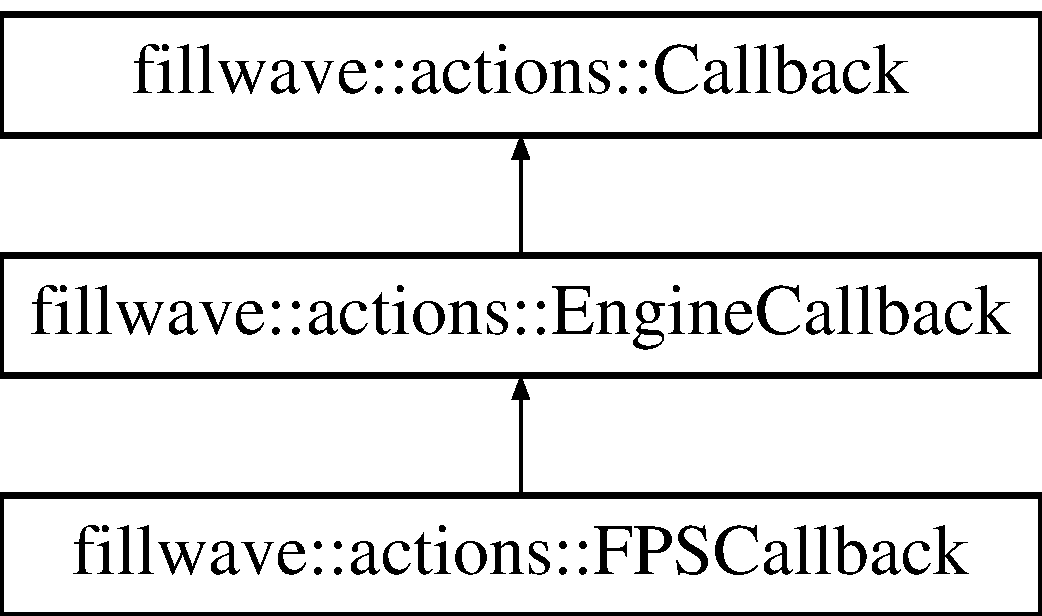
\includegraphics[height=3.000000cm]{classfillwave_1_1actions_1_1EngineCallback}
\end{center}
\end{figure}
\subsection*{Public Member Functions}
\begin{DoxyCompactItemize}
\item 
\hypertarget{classfillwave_1_1actions_1_1EngineCallback_acf1ee572444c1c6d8d78566c05b66b83}{}{\bfseries Engine\+Callback} (e\+Event\+Type event\+Type)\label{classfillwave_1_1actions_1_1EngineCallback_acf1ee572444c1c6d8d78566c05b66b83}

\item 
\hypertarget{classfillwave_1_1actions_1_1EngineCallback_a0699b0bc6f2d598b0192c1f8e486483a}{}virtual void {\bfseries perform} (\hyperlink{classfillwave_1_1Engine}{Engine} $\ast$engine, \hyperlink{classfillwave_1_1actions_1_1EventType}{Event\+Type} $\ast$event\+Type)=0\label{classfillwave_1_1actions_1_1EngineCallback_a0699b0bc6f2d598b0192c1f8e486483a}

\end{DoxyCompactItemize}


\subsection{Detailed Description}
Base for engine-\/aware callbacks. 

The documentation for this class was generated from the following file\+:\begin{DoxyCompactItemize}
\item 
/home/filip/\+Projects/fillwave/inc/fillwave/actions/Engine\+Callback.\+h\end{DoxyCompactItemize}

\hypertarget{structfillwave_1_1Engine_1_1EngineImpl}{}\section{fillwave\+:\+:Engine\+:\+:Engine\+Impl Struct Reference}
\label{structfillwave_1_1Engine_1_1EngineImpl}\index{fillwave\+::\+Engine\+::\+Engine\+Impl@{fillwave\+::\+Engine\+::\+Engine\+Impl}}
\subsection*{Public Member Functions}
\begin{DoxyCompactItemize}
\item 
\hypertarget{structfillwave_1_1Engine_1_1EngineImpl_a6c76291596614e9197fd6bce3504719a}{}{\bfseries Engine\+Impl} (\hyperlink{classfillwave_1_1Engine}{Engine} $\ast$engine, G\+Lint argc, G\+Lchar $\ast$const argv\mbox{[}$\,$\mbox{]})\label{structfillwave_1_1Engine_1_1EngineImpl_a6c76291596614e9197fd6bce3504719a}

\item 
\hypertarget{structfillwave_1_1Engine_1_1EngineImpl_a3dd4c55ebb97c77dfabbcc712eb91955}{}void {\bfseries run\+Callbacks} (std\+::vector$<$ \hyperlink{classfillwave_1_1actions_1_1EngineCallback}{actions\+::\+Engine\+Callback} $\ast$ $>$ \&callbacks, \hyperlink{classfillwave_1_1actions_1_1EventType}{actions\+::\+Event\+Type} $\ast$event)\label{structfillwave_1_1Engine_1_1EngineImpl_a3dd4c55ebb97c77dfabbcc712eb91955}

\item 
\hypertarget{structfillwave_1_1Engine_1_1EngineImpl_a4dbaa280c45297e1cb25ee71d039fb08}{}void {\bfseries clear\+Callbacks} (std\+::vector$<$ \hyperlink{classfillwave_1_1actions_1_1EngineCallback}{actions\+::\+Engine\+Callback} $\ast$ $>$ \&callbacks)\label{structfillwave_1_1Engine_1_1EngineImpl_a4dbaa280c45297e1cb25ee71d039fb08}

\item 
\hypertarget{structfillwave_1_1Engine_1_1EngineImpl_a1ed150cea5ab2fb1d4c8df17bb2ac950}{}void {\bfseries unregister\+Callback} (std\+::vector$<$ \hyperlink{classfillwave_1_1actions_1_1EngineCallback}{actions\+::\+Engine\+Callback} $\ast$ $>$ \&callbacks, \hyperlink{classfillwave_1_1actions_1_1EngineCallback}{actions\+::\+Engine\+Callback} $\ast$callback)\label{structfillwave_1_1Engine_1_1EngineImpl_a1ed150cea5ab2fb1d4c8df17bb2ac950}

\item 
\hypertarget{structfillwave_1_1Engine_1_1EngineImpl_aeed21a166f13fbd4ef783db853836750}{}void {\bfseries evaluate\+Shadow\+Maps} ()\label{structfillwave_1_1Engine_1_1EngineImpl_aeed21a166f13fbd4ef783db853836750}

\item 
\hypertarget{structfillwave_1_1Engine_1_1EngineImpl_aa5696e94c61d393ce2e32c7a048766ae}{}void {\bfseries evaluate\+Debugger} ()\label{structfillwave_1_1Engine_1_1EngineImpl_aa5696e94c61d393ce2e32c7a048766ae}

\item 
\hypertarget{structfillwave_1_1Engine_1_1EngineImpl_afefed0cc80ec702b0a1c3bfeebe8fd77}{}void {\bfseries evaluate\+Dynamic\+Textures} (G\+Lfloat time\+Expired\+In\+Seconds)\label{structfillwave_1_1Engine_1_1EngineImpl_afefed0cc80ec702b0a1c3bfeebe8fd77}

\item 
\hypertarget{structfillwave_1_1Engine_1_1EngineImpl_a722669bb4811a36694509ac06d8226f9}{}void {\bfseries evaluate\+Time} (G\+Lfloat time\+Expired\+In\+Seconds)\label{structfillwave_1_1Engine_1_1EngineImpl_a722669bb4811a36694509ac06d8226f9}

\item 
\hypertarget{structfillwave_1_1Engine_1_1EngineImpl_aa58cc946ce4337587824b6ea882bbe76}{}void {\bfseries evaluate\+Startup\+Animation} (G\+Lfloat time)\label{structfillwave_1_1Engine_1_1EngineImpl_aa58cc946ce4337587824b6ea882bbe76}

\item 
\hypertarget{structfillwave_1_1Engine_1_1EngineImpl_a82edf3e5ad93b78b9ed9756b30c3b49d}{}void {\bfseries draw} (G\+Lfloat time)\label{structfillwave_1_1Engine_1_1EngineImpl_a82edf3e5ad93b78b9ed9756b30c3b49d}

\item 
\hypertarget{structfillwave_1_1Engine_1_1EngineImpl_a69ced5fe8d88e68185a82a6e6c404006}{}void {\bfseries draw\+Lines} (G\+Lfloat time)\label{structfillwave_1_1Engine_1_1EngineImpl_a69ced5fe8d88e68185a82a6e6c404006}

\item 
\hypertarget{structfillwave_1_1Engine_1_1EngineImpl_a588293236606e4c021f538658e4def60}{}void {\bfseries draw\+Points} (G\+Lfloat time)\label{structfillwave_1_1Engine_1_1EngineImpl_a588293236606e4c021f538658e4def60}

\item 
\hypertarget{structfillwave_1_1Engine_1_1EngineImpl_abda6fbb942630c3eeaf2b4e1c63b77a1}{}void {\bfseries draw\+Texture} (\hyperlink{classfillwave_1_1core_1_1Texture}{core\+::\+Texture} $\ast$t, \hyperlink{classfillwave_1_1core_1_1Program}{core\+::\+Program} $\ast$p)\label{structfillwave_1_1Engine_1_1EngineImpl_abda6fbb942630c3eeaf2b4e1c63b77a1}

\item 
\hypertarget{structfillwave_1_1Engine_1_1EngineImpl_a230b13dd29c3d171d0ebf95d5b85e2a4}{}void {\bfseries draw\+Texture} (\hyperlink{classfillwave_1_1core_1_1Texture}{core\+::\+Texture} $\ast$t)\label{structfillwave_1_1Engine_1_1EngineImpl_a230b13dd29c3d171d0ebf95d5b85e2a4}

\item 
\hypertarget{structfillwave_1_1Engine_1_1EngineImpl_a12855c0e5ffe2457c388f3b65107d9cc}{}void {\bfseries draw\+Clear} ()\label{structfillwave_1_1Engine_1_1EngineImpl_a12855c0e5ffe2457c388f3b65107d9cc}

\item 
\hypertarget{structfillwave_1_1Engine_1_1EngineImpl_a9a937874128372b4a0cf28d18ff432f2}{}void {\bfseries draw\+Scene} (G\+Lfloat time)\label{structfillwave_1_1Engine_1_1EngineImpl_a9a937874128372b4a0cf28d18ff432f2}

\item 
\hypertarget{structfillwave_1_1Engine_1_1EngineImpl_ab82c35f1b2f649341360f0c6736621b1}{}void {\bfseries draw\+Scene\+Startup} ()\label{structfillwave_1_1Engine_1_1EngineImpl_ab82c35f1b2f649341360f0c6736621b1}

\item 
\hypertarget{structfillwave_1_1Engine_1_1EngineImpl_a6f995bcb8153e8f7ae6419587d3a5f41}{}void {\bfseries draw\+Scene\+Core} ()\label{structfillwave_1_1Engine_1_1EngineImpl_a6f995bcb8153e8f7ae6419587d3a5f41}

\item 
\hypertarget{structfillwave_1_1Engine_1_1EngineImpl_a2ba681bb6af63e1ade56399e06fdd5f2}{}void {\bfseries draw\+Scene\+Core\+F\+R} ()\label{structfillwave_1_1Engine_1_1EngineImpl_a2ba681bb6af63e1ade56399e06fdd5f2}

\item 
\hypertarget{structfillwave_1_1Engine_1_1EngineImpl_a3a677169d9eab4627e4fa3e47789eb8e}{}void {\bfseries draw\+Scene\+Core\+D\+R} ()\label{structfillwave_1_1Engine_1_1EngineImpl_a3a677169d9eab4627e4fa3e47789eb8e}

\item 
\hypertarget{structfillwave_1_1Engine_1_1EngineImpl_a3d5f368b0befb801f49441abdc9849d8}{}void {\bfseries draw\+Text} ()\label{structfillwave_1_1Engine_1_1EngineImpl_a3d5f368b0befb801f49441abdc9849d8}

\item 
\hypertarget{structfillwave_1_1Engine_1_1EngineImpl_ab6b707a9b61f7a8859032f45252df4f8}{}void {\bfseries draw\+Geometry\+Pass} ()\label{structfillwave_1_1Engine_1_1EngineImpl_ab6b707a9b61f7a8859032f45252df4f8}

\item 
\hypertarget{structfillwave_1_1Engine_1_1EngineImpl_a2896d5491097b4d6d79a9af88a907a1d}{}void {\bfseries draw\+Occlusion\+Pass} ()\label{structfillwave_1_1Engine_1_1EngineImpl_a2896d5491097b4d6d79a9af88a907a1d}

\item 
\hypertarget{structfillwave_1_1Engine_1_1EngineImpl_a690196b3cf17c2315c9fd691b456a452}{}void {\bfseries draw\+Depthless\+Pass} ()\label{structfillwave_1_1Engine_1_1EngineImpl_a690196b3cf17c2315c9fd691b456a452}

\item 
\hypertarget{structfillwave_1_1Engine_1_1EngineImpl_a5b66b89d82857b57745fd04d4360a30a}{}void {\bfseries draw\+Ambient\+Pass} ()\label{structfillwave_1_1Engine_1_1EngineImpl_a5b66b89d82857b57745fd04d4360a30a}

\item 
\hypertarget{structfillwave_1_1Engine_1_1EngineImpl_a44a9ed999d42baee3088db2dc3d035e9}{}void {\bfseries draw\+A\+O\+Pass} ()\label{structfillwave_1_1Engine_1_1EngineImpl_a44a9ed999d42baee3088db2dc3d035e9}

\item 
\hypertarget{structfillwave_1_1Engine_1_1EngineImpl_ae44d13e7727298978931fc0194757ef3}{}void {\bfseries draw\+Color\+Pass} ()\label{structfillwave_1_1Engine_1_1EngineImpl_ae44d13e7727298978931fc0194757ef3}

\item 
\hypertarget{structfillwave_1_1Engine_1_1EngineImpl_ac1f73527fb62e97d5dad344cee0c8d39}{}void {\bfseries draw\+Lights\+Spot\+Pass} (G\+Lint \&texture\+Unit)\label{structfillwave_1_1Engine_1_1EngineImpl_ac1f73527fb62e97d5dad344cee0c8d39}

\item 
\hypertarget{structfillwave_1_1Engine_1_1EngineImpl_a55ce42ae579120d2e9b6288615e59944}{}void {\bfseries draw\+Lights\+Directional\+Pass} (G\+Lint \&texture\+Unit)\label{structfillwave_1_1Engine_1_1EngineImpl_a55ce42ae579120d2e9b6288615e59944}

\item 
\hypertarget{structfillwave_1_1Engine_1_1EngineImpl_abe254a80f34cc134b8c30fa553f70522}{}void {\bfseries draw\+Lights\+Point\+Pass} (G\+Lint \&texture\+Unit)\label{structfillwave_1_1Engine_1_1EngineImpl_abe254a80f34cc134b8c30fa553f70522}

\item 
\hypertarget{structfillwave_1_1Engine_1_1EngineImpl_a7b1f3dc244c87e91a53f4099ea595417}{}void {\bfseries draw\+Color\+Pass\+Begin} ()\label{structfillwave_1_1Engine_1_1EngineImpl_a7b1f3dc244c87e91a53f4099ea595417}

\item 
\hypertarget{structfillwave_1_1Engine_1_1EngineImpl_aa7f987143c09c27f6d98470c9ebadf60}{}void {\bfseries draw\+Color\+Pass\+End} ()\label{structfillwave_1_1Engine_1_1EngineImpl_aa7f987143c09c27f6d98470c9ebadf60}

\item 
\hypertarget{structfillwave_1_1Engine_1_1EngineImpl_aeaa89cb8d068ccf8e7404fa0d6682024}{}p\+Shader {\bfseries store\+Shader} (const std\+::string \&shader\+Path, const G\+Luint \&shader\+Type)\label{structfillwave_1_1Engine_1_1EngineImpl_aeaa89cb8d068ccf8e7404fa0d6682024}

\item 
\hypertarget{structfillwave_1_1Engine_1_1EngineImpl_ab676c0581fffada7c179aa188e9b5a37}{}p\+Shader {\bfseries store\+Shader} (const std\+::string \&shader\+Name, const G\+Luint \&shader\+Type, const std\+::string \&shader\+Source)\label{structfillwave_1_1Engine_1_1EngineImpl_ab676c0581fffada7c179aa188e9b5a37}

\item 
\hypertarget{structfillwave_1_1Engine_1_1EngineImpl_a993f079d8688f6e9d647fb9d8c861a31}{}glm\+::ivec4 {\bfseries picking\+Buffer\+Get\+Color} (G\+Lubyte $\ast$data, G\+Luint x, G\+Luint y)\label{structfillwave_1_1Engine_1_1EngineImpl_a993f079d8688f6e9d647fb9d8c861a31}

\item 
\hypertarget{structfillwave_1_1Engine_1_1EngineImpl_a677027e42098fba43736efb0f9565e4b}{}void {\bfseries init} ()\label{structfillwave_1_1Engine_1_1EngineImpl_a677027e42098fba43736efb0f9565e4b}

\item 
\hypertarget{structfillwave_1_1Engine_1_1EngineImpl_a50f486d35afbff9cb79cf658037da4a8}{}void {\bfseries init\+Extensions} ()\label{structfillwave_1_1Engine_1_1EngineImpl_a50f486d35afbff9cb79cf658037da4a8}

\item 
\hypertarget{structfillwave_1_1Engine_1_1EngineImpl_ab65e9b93533e6bdbec741485ce8a3714}{}void {\bfseries init\+Context} ()\label{structfillwave_1_1Engine_1_1EngineImpl_ab65e9b93533e6bdbec741485ce8a3714}

\item 
\hypertarget{structfillwave_1_1Engine_1_1EngineImpl_ada68b25e7af386ad0049d3125a670d66}{}void {\bfseries init\+Picking\+Buffer} ()\label{structfillwave_1_1Engine_1_1EngineImpl_ada68b25e7af386ad0049d3125a670d66}

\item 
\hypertarget{structfillwave_1_1Engine_1_1EngineImpl_afc91d2ecbd80f4ec48c0eb34cce1d43a}{}void {\bfseries init\+Pipelines} ()\label{structfillwave_1_1Engine_1_1EngineImpl_afc91d2ecbd80f4ec48c0eb34cce1d43a}

\item 
\hypertarget{structfillwave_1_1Engine_1_1EngineImpl_a8d4401a3384dca6c1f1136ddc495ff86}{}void {\bfseries init\+Uniforms} ()\label{structfillwave_1_1Engine_1_1EngineImpl_a8d4401a3384dca6c1f1136ddc495ff86}

\item 
\hypertarget{structfillwave_1_1Engine_1_1EngineImpl_acb3a9e74e46b974bc5d7633d978f23ab}{}void {\bfseries init\+Management} ()\label{structfillwave_1_1Engine_1_1EngineImpl_acb3a9e74e46b974bc5d7633d978f23ab}

\item 
\hypertarget{structfillwave_1_1Engine_1_1EngineImpl_a97583b128b61bbe4bca8efcfaaf7fd11}{}void {\bfseries init\+Deferred\+Shading} ()\label{structfillwave_1_1Engine_1_1EngineImpl_a97583b128b61bbe4bca8efcfaaf7fd11}

\item 
\hypertarget{structfillwave_1_1Engine_1_1EngineImpl_ab6ca32c01acb113d904b2dc69e6ad1f7}{}void {\bfseries init\+Ambient\+Occlusion} ()\label{structfillwave_1_1Engine_1_1EngineImpl_ab6ca32c01acb113d904b2dc69e6ad1f7}

\item 
\hypertarget{structfillwave_1_1Engine_1_1EngineImpl_a502cc7670e262542798cc01c9de6c8c1}{}void {\bfseries init\+Geometry\+Buffer} ()\label{structfillwave_1_1Engine_1_1EngineImpl_a502cc7670e262542798cc01c9de6c8c1}

\item 
\hypertarget{structfillwave_1_1Engine_1_1EngineImpl_a4671b46a5295cebbd9d8cdd7bdc64ab3}{}void {\bfseries init\+Extras} ()\label{structfillwave_1_1Engine_1_1EngineImpl_a4671b46a5295cebbd9d8cdd7bdc64ab3}

\item 
\hypertarget{structfillwave_1_1Engine_1_1EngineImpl_af52e19bf4630074f150e635919417d53}{}void {\bfseries init\+Occlusion\+Test} ()\label{structfillwave_1_1Engine_1_1EngineImpl_af52e19bf4630074f150e635919417d53}

\item 
\hypertarget{structfillwave_1_1Engine_1_1EngineImpl_aa0ce368354e4fc6e763b0bd9028d384e}{}void {\bfseries init\+Uniforms\+Cache} ()\label{structfillwave_1_1Engine_1_1EngineImpl_aa0ce368354e4fc6e763b0bd9028d384e}

\item 
\hypertarget{structfillwave_1_1Engine_1_1EngineImpl_a7794b9d721ef504c8e0079e538ce213d}{}void {\bfseries init\+Startup} ()\label{structfillwave_1_1Engine_1_1EngineImpl_a7794b9d721ef504c8e0079e538ce213d}

\item 
\hypertarget{structfillwave_1_1Engine_1_1EngineImpl_a66dac6a37a653db98e30adef7de3850a}{}void {\bfseries init\+Geometry\+Shading} ()\label{structfillwave_1_1Engine_1_1EngineImpl_a66dac6a37a653db98e30adef7de3850a}

\item 
\hypertarget{structfillwave_1_1Engine_1_1EngineImpl_a5691ec3bd35bf65e841cdb16cd83667d}{}void {\bfseries reload} ()\label{structfillwave_1_1Engine_1_1EngineImpl_a5691ec3bd35bf65e841cdb16cd83667d}

\item 
\hypertarget{structfillwave_1_1Engine_1_1EngineImpl_aeb0ec4eb1da84a0fbefb3c283c47300a}{}void {\bfseries reload\+Picking\+Buffer} ()\label{structfillwave_1_1Engine_1_1EngineImpl_aeb0ec4eb1da84a0fbefb3c283c47300a}

\item 
\hypertarget{structfillwave_1_1Engine_1_1EngineImpl_af245d3daa135993c76d40c3e4fc450f6}{}void {\bfseries reload\+Geometry\+Buffer} ()\label{structfillwave_1_1Engine_1_1EngineImpl_af245d3daa135993c76d40c3e4fc450f6}

\item 
\hypertarget{structfillwave_1_1Engine_1_1EngineImpl_a4f48c92602eebbc0e2117ee6ff409016}{}void {\bfseries insert\+Resize\+Screen} (G\+Luint width, G\+Luint height)\label{structfillwave_1_1Engine_1_1EngineImpl_a4f48c92602eebbc0e2117ee6ff409016}

\item 
\hypertarget{structfillwave_1_1Engine_1_1EngineImpl_ae4305e7e95e904d4d631605c9ce2a347}{}p\+Sampler {\bfseries store\+S\+O} (G\+Lint texture\+Unit)\label{structfillwave_1_1Engine_1_1EngineImpl_ae4305e7e95e904d4d631605c9ce2a347}

\item 
\hypertarget{structfillwave_1_1Engine_1_1EngineImpl_a79a5f7b2f4fde0f99d76448aa05baf48}{}p\+Vertex\+Array {\bfseries store\+V\+A\+O} (\hyperlink{classfillwave_1_1models_1_1Reloadable}{models\+::\+Reloadable} $\ast$user=nullptr)\label{structfillwave_1_1Engine_1_1EngineImpl_a79a5f7b2f4fde0f99d76448aa05baf48}

\end{DoxyCompactItemize}
\subsection*{Public Attributes}
\begin{DoxyCompactItemize}
\item 
\hypertarget{structfillwave_1_1Engine_1_1EngineImpl_a88f49dc2a2f91db6fef013e6fe5f4c07}{}\hyperlink{classfillwave_1_1Engine}{Engine} $\ast$ {\bfseries m\+Engine}\label{structfillwave_1_1Engine_1_1EngineImpl_a88f49dc2a2f91db6fef013e6fe5f4c07}

\item 
\hypertarget{structfillwave_1_1Engine_1_1EngineImpl_ac565498c52570520e8468ba0f2785d13}{}Assimp\+::\+Importer {\bfseries m\+Importer}\label{structfillwave_1_1Engine_1_1EngineImpl_ac565498c52570520e8468ba0f2785d13}

\item 
\hypertarget{structfillwave_1_1Engine_1_1EngineImpl_ae2691f3b1f1b15b80c76cbe3950a87d4}{}G\+Luint {\bfseries m\+Window\+Width} = 1920\label{structfillwave_1_1Engine_1_1EngineImpl_ae2691f3b1f1b15b80c76cbe3950a87d4}

\item 
\hypertarget{structfillwave_1_1Engine_1_1EngineImpl_a362b6a1ee3eb14b4f80e68e2736fd1cb}{}G\+Luint {\bfseries m\+Window\+Height} = 1200\label{structfillwave_1_1Engine_1_1EngineImpl_a362b6a1ee3eb14b4f80e68e2736fd1cb}

\item 
\hypertarget{structfillwave_1_1Engine_1_1EngineImpl_a001acb1c7ea7a13dd31b22461ec482b5}{}G\+Lfloat {\bfseries m\+Startup\+Time}\label{structfillwave_1_1Engine_1_1EngineImpl_a001acb1c7ea7a13dd31b22461ec482b5}

\item 
\hypertarget{structfillwave_1_1Engine_1_1EngineImpl_a854e82aaf53e54b34d9ee9c10200e9e8}{}p\+Texture {\bfseries m\+Startup\+Texture}\label{structfillwave_1_1Engine_1_1EngineImpl_a854e82aaf53e54b34d9ee9c10200e9e8}

\item 
\hypertarget{structfillwave_1_1Engine_1_1EngineImpl_aca249e6321d92809589c805e92388490}{}const G\+Lfloat {\bfseries m\+Startup\+Time\+Limit} = 8.\+0f\label{structfillwave_1_1Engine_1_1EngineImpl_aca249e6321d92809589c805e92388490}

\item 
\hypertarget{structfillwave_1_1Engine_1_1EngineImpl_a3f7ca8d7fc0aaf680159494aa177a3c2}{}pu\+Post\+Processing\+Pass {\bfseries m\+Post\+Processing\+Pass\+Startup}\label{structfillwave_1_1Engine_1_1EngineImpl_a3f7ca8d7fc0aaf680159494aa177a3c2}

\item 
\hypertarget{structfillwave_1_1Engine_1_1EngineImpl_a95521c91ef03bb50d35de76675c685ad}{}G\+Lboolean {\bfseries m\+Is\+D\+R}\label{structfillwave_1_1Engine_1_1EngineImpl_a95521c91ef03bb50d35de76675c685ad}

\item 
\hypertarget{structfillwave_1_1Engine_1_1EngineImpl_a907fd1a985795f13e77c507e9fe2e96c}{}G\+Lboolean {\bfseries m\+Is\+A\+O}\label{structfillwave_1_1Engine_1_1EngineImpl_a907fd1a985795f13e77c507e9fe2e96c}

\item 
\hypertarget{structfillwave_1_1Engine_1_1EngineImpl_a1d568b9191bc55b17df458564c1005c6}{}G\+Lboolean {\bfseries m\+I\+S\+O\+Q}\label{structfillwave_1_1Engine_1_1EngineImpl_a1d568b9191bc55b17df458564c1005c6}

\item 
\hypertarget{structfillwave_1_1Engine_1_1EngineImpl_a859312810c07e17ff21e2ed1e32fd1ff}{}p\+Scene {\bfseries m\+Scene}\label{structfillwave_1_1Engine_1_1EngineImpl_a859312810c07e17ff21e2ed1e32fd1ff}

\item 
\hypertarget{structfillwave_1_1Engine_1_1EngineImpl_acedb3775403c996dadcdc9ecc0ee8952}{}glm\+::vec3 {\bfseries m\+Background\+Color}\label{structfillwave_1_1Engine_1_1EngineImpl_acedb3775403c996dadcdc9ecc0ee8952}

\item 
\hypertarget{structfillwave_1_1Engine_1_1EngineImpl_a8935fec9cccf405a4730c5b9836a7e5d}{}\hyperlink{classfillwave_1_1loader_1_1FontLoader}{loader\+::\+Font\+Loader} {\bfseries m\+Font\+Loader}\label{structfillwave_1_1Engine_1_1EngineImpl_a8935fec9cccf405a4730c5b9836a7e5d}

\item 
\hypertarget{structfillwave_1_1Engine_1_1EngineImpl_ac3a7a0e29ff249049382c446ec4d4bc9}{}\hyperlink{classfillwave_1_1loader_1_1FileLoader}{loader\+::\+File\+Loader} {\bfseries m\+File\+Loader}\label{structfillwave_1_1Engine_1_1EngineImpl_ac3a7a0e29ff249049382c446ec4d4bc9}

\item 
\hypertarget{structfillwave_1_1Engine_1_1EngineImpl_a88b30b7bcc34a21e3a561284b76315a6}{}\hyperlink{classfillwave_1_1loader_1_1ProgramLoader}{loader\+::\+Program\+Loader} {\bfseries m\+Program\+Loader}\label{structfillwave_1_1Engine_1_1EngineImpl_a88b30b7bcc34a21e3a561284b76315a6}

\item 
\hypertarget{structfillwave_1_1Engine_1_1EngineImpl_adf63c8046fda46607233443a8c6353a8}{}p\+Texture2\+D\+Renderable {\bfseries m\+Picking\+Renderable\+Texture}\label{structfillwave_1_1Engine_1_1EngineImpl_adf63c8046fda46607233443a8c6353a8}

\item 
\hypertarget{structfillwave_1_1Engine_1_1EngineImpl_a0095e15205f86bedee9a2ca9333178a3}{}pu\+Pixel\+Buffer {\bfseries m\+Picking\+Pixel\+Buffer}\label{structfillwave_1_1Engine_1_1EngineImpl_a0095e15205f86bedee9a2ca9333178a3}

\item 
\hypertarget{structfillwave_1_1Engine_1_1EngineImpl_a65937bb5de56c774f99458643fce11c3}{}pu\+Program\+Manager {\bfseries m\+Program\+Manager}\label{structfillwave_1_1Engine_1_1EngineImpl_a65937bb5de56c774f99458643fce11c3}

\item 
\hypertarget{structfillwave_1_1Engine_1_1EngineImpl_ad0640e410c604a0b89582b23b6dc2352}{}pu\+Texture\+Manager {\bfseries m\+Texture\+Manager}\label{structfillwave_1_1Engine_1_1EngineImpl_ad0640e410c604a0b89582b23b6dc2352}

\item 
\hypertarget{structfillwave_1_1Engine_1_1EngineImpl_a4d0ff758ff60cee62cb5eaf058f42c99}{}pu\+Shader\+Manager {\bfseries m\+Shader\+Manager}\label{structfillwave_1_1Engine_1_1EngineImpl_a4d0ff758ff60cee62cb5eaf058f42c99}

\item 
\hypertarget{structfillwave_1_1Engine_1_1EngineImpl_ab1efcecba5a16834da7551d378e6c1ba}{}pu\+Light\+Manager {\bfseries m\+Light\+Manager}\label{structfillwave_1_1Engine_1_1EngineImpl_ab1efcecba5a16834da7551d378e6c1ba}

\item 
\hypertarget{structfillwave_1_1Engine_1_1EngineImpl_a4f19c79e22357eff6c40a1f130592dcf}{}pu\+Sampler\+Manager {\bfseries m\+Sampler\+Manager}\label{structfillwave_1_1Engine_1_1EngineImpl_a4f19c79e22357eff6c40a1f130592dcf}

\item 
\hypertarget{structfillwave_1_1Engine_1_1EngineImpl_a84ea194784cf3070bdbf85c497dd472c}{}pu\+Buffer\+Manager {\bfseries m\+Buffer\+Manager}\label{structfillwave_1_1Engine_1_1EngineImpl_a84ea194784cf3070bdbf85c497dd472c}

\item 
\hypertarget{structfillwave_1_1Engine_1_1EngineImpl_abf005f51f8e20185a89110392049b6e4}{}std\+::vector$<$ p\+Text $>$ {\bfseries m\+Text\+Manager}\label{structfillwave_1_1Engine_1_1EngineImpl_abf005f51f8e20185a89110392049b6e4}

\item 
\hypertarget{structfillwave_1_1Engine_1_1EngineImpl_af51024a18ced13ea136e28ecd774267f}{}std\+::vector$<$ p\+Font $>$ {\bfseries m\+Font\+Manager}\label{structfillwave_1_1Engine_1_1EngineImpl_af51024a18ced13ea136e28ecd774267f}

\item 
\hypertarget{structfillwave_1_1Engine_1_1EngineImpl_ab83af8dffddf67dd50a37dd1590baf18}{}std\+::vector$<$ \hyperlink{classfillwave_1_1common_1_1PostProcessingPass}{common\+::\+Post\+Processing\+Pass} $>$ {\bfseries m\+Post\+Processing\+Passes}\label{structfillwave_1_1Engine_1_1EngineImpl_ab83af8dffddf67dd50a37dd1590baf18}

\item 
\hypertarget{structfillwave_1_1Engine_1_1EngineImpl_ac1231a2a86b2c3cfe8b9f7b9440f89bf}{}std\+::vector$<$ p\+Texture2\+D\+Renderable\+Dynamic $>$ {\bfseries m\+Textures\+Dynamic}\label{structfillwave_1_1Engine_1_1EngineImpl_ac1231a2a86b2c3cfe8b9f7b9440f89bf}

\item 
\hypertarget{structfillwave_1_1Engine_1_1EngineImpl_a2e5b973e0fdb2a12228ab29291f2baf6}{}p\+Program {\bfseries m\+Program\+Texture\+Lookup}\label{structfillwave_1_1Engine_1_1EngineImpl_a2e5b973e0fdb2a12228ab29291f2baf6}

\item 
\hypertarget{structfillwave_1_1Engine_1_1EngineImpl_a7a30b84cb2c3ad1e49c918dc5b6335ef}{}pu\+Fence {\bfseries m\+Fence}\label{structfillwave_1_1Engine_1_1EngineImpl_a7a30b84cb2c3ad1e49c918dc5b6335ef}

\item 
\hypertarget{structfillwave_1_1Engine_1_1EngineImpl_a6ec45f07412f6770a7075286dd8349f2}{}pu\+Framebuffer\+Geometry {\bfseries m\+G\+Buffer}\label{structfillwave_1_1Engine_1_1EngineImpl_a6ec45f07412f6770a7075286dd8349f2}

\item 
\hypertarget{structfillwave_1_1Engine_1_1EngineImpl_ae7d51a4fba6bdedeccd1e41cfca3a60a}{}p\+Program {\bfseries m\+Program\+D\+R\+Spot\+Light}\label{structfillwave_1_1Engine_1_1EngineImpl_ae7d51a4fba6bdedeccd1e41cfca3a60a}

\item 
\hypertarget{structfillwave_1_1Engine_1_1EngineImpl_a8dbbb4680f6a462c11d5201b9431043c}{}p\+Program {\bfseries m\+Program\+D\+R\+Direcional\+Light}\label{structfillwave_1_1Engine_1_1EngineImpl_a8dbbb4680f6a462c11d5201b9431043c}

\item 
\hypertarget{structfillwave_1_1Engine_1_1EngineImpl_ada796d07813b6976c5a31ca6ebe8b95d}{}p\+Program {\bfseries m\+Program\+D\+R\+Point\+Light}\label{structfillwave_1_1Engine_1_1EngineImpl_ada796d07813b6976c5a31ca6ebe8b95d}

\item 
\hypertarget{structfillwave_1_1Engine_1_1EngineImpl_ae187ee4233ba11d01ca6c553ffb0a292}{}p\+Program {\bfseries m\+Program\+D\+R\+Depthless}\label{structfillwave_1_1Engine_1_1EngineImpl_ae187ee4233ba11d01ca6c553ffb0a292}

\item 
\hypertarget{structfillwave_1_1Engine_1_1EngineImpl_a8c526937923bc41a7d6d2bc0853f78a0}{}p\+Program {\bfseries m\+Program\+D\+R\+Ambient}\label{structfillwave_1_1Engine_1_1EngineImpl_a8c526937923bc41a7d6d2bc0853f78a0}

\item 
\hypertarget{structfillwave_1_1Engine_1_1EngineImpl_a9de5a895c980dfd64875335bc2eebe7e}{}G\+Lint {\bfseries m\+U\+L\+C\+Camera\+Position\+Spot}\label{structfillwave_1_1Engine_1_1EngineImpl_a9de5a895c980dfd64875335bc2eebe7e}

\item 
\hypertarget{structfillwave_1_1Engine_1_1EngineImpl_a775d9fc089a18b64a63da726e9138823}{}G\+Lint {\bfseries m\+U\+L\+C\+Ambient\+Intensity\+Spot}\label{structfillwave_1_1Engine_1_1EngineImpl_a775d9fc089a18b64a63da726e9138823}

\item 
\hypertarget{structfillwave_1_1Engine_1_1EngineImpl_a601c8d3c1affa8f8f2628bcc8f9580ab}{}G\+Lint {\bfseries m\+U\+L\+C\+Screen\+Size\+Spot}\label{structfillwave_1_1Engine_1_1EngineImpl_a601c8d3c1affa8f8f2628bcc8f9580ab}

\item 
\hypertarget{structfillwave_1_1Engine_1_1EngineImpl_abfe1419eeb394c4f8d067be35bdb2e4b}{}G\+Lint {\bfseries m\+U\+L\+C\+Shadow\+Unit\+Spot}\label{structfillwave_1_1Engine_1_1EngineImpl_abfe1419eeb394c4f8d067be35bdb2e4b}

\item 
\hypertarget{structfillwave_1_1Engine_1_1EngineImpl_af01bda565467bb3db35a7350508b0adb}{}G\+Lint {\bfseries m\+U\+L\+C\+Is\+A\+O\+Spot}\label{structfillwave_1_1Engine_1_1EngineImpl_af01bda565467bb3db35a7350508b0adb}

\item 
\hypertarget{structfillwave_1_1Engine_1_1EngineImpl_a98b80309ea05dd8492ad7a9be40b1123}{}G\+Lint {\bfseries m\+U\+L\+C\+Camera\+Position\+Directional}\label{structfillwave_1_1Engine_1_1EngineImpl_a98b80309ea05dd8492ad7a9be40b1123}

\item 
\hypertarget{structfillwave_1_1Engine_1_1EngineImpl_a55599aa869de70dd2cc9c3057d2e55df}{}G\+Lint {\bfseries m\+U\+L\+C\+Ambient\+Intensity\+Directional}\label{structfillwave_1_1Engine_1_1EngineImpl_a55599aa869de70dd2cc9c3057d2e55df}

\item 
\hypertarget{structfillwave_1_1Engine_1_1EngineImpl_a771bf5ae5e7022bb5f291cf2d5d3a762}{}G\+Lint {\bfseries m\+U\+L\+C\+Screen\+Size\+Directional}\label{structfillwave_1_1Engine_1_1EngineImpl_a771bf5ae5e7022bb5f291cf2d5d3a762}

\item 
\hypertarget{structfillwave_1_1Engine_1_1EngineImpl_a980aab610c34e1630d013decfe59fc4b}{}G\+Lint {\bfseries m\+U\+L\+C\+Shadow\+Unit\+Directional}\label{structfillwave_1_1Engine_1_1EngineImpl_a980aab610c34e1630d013decfe59fc4b}

\item 
\hypertarget{structfillwave_1_1Engine_1_1EngineImpl_a2d0b86de29a37d688488a753d515094d}{}G\+Lint {\bfseries m\+U\+L\+C\+Is\+A\+O\+Directional}\label{structfillwave_1_1Engine_1_1EngineImpl_a2d0b86de29a37d688488a753d515094d}

\item 
\hypertarget{structfillwave_1_1Engine_1_1EngineImpl_a574ec7a9933eb0c31ee7820af18b3cf7}{}G\+Lint {\bfseries m\+U\+L\+C\+Camera\+Position\+Point}\label{structfillwave_1_1Engine_1_1EngineImpl_a574ec7a9933eb0c31ee7820af18b3cf7}

\item 
\hypertarget{structfillwave_1_1Engine_1_1EngineImpl_a15d737e819582487c24594863dec8bfd}{}G\+Lint {\bfseries m\+U\+L\+C\+Ambient\+Intensity\+Point}\label{structfillwave_1_1Engine_1_1EngineImpl_a15d737e819582487c24594863dec8bfd}

\item 
\hypertarget{structfillwave_1_1Engine_1_1EngineImpl_a37ec995c1da0203b29a8182b3c619103}{}G\+Lint {\bfseries m\+U\+L\+C\+M\+V\+P\+Point}\label{structfillwave_1_1Engine_1_1EngineImpl_a37ec995c1da0203b29a8182b3c619103}

\item 
\hypertarget{structfillwave_1_1Engine_1_1EngineImpl_aef8f01747a28482ad7ddd1d002219955}{}G\+Lint {\bfseries m\+U\+L\+C\+Screen\+Size\+Point}\label{structfillwave_1_1Engine_1_1EngineImpl_aef8f01747a28482ad7ddd1d002219955}

\item 
\hypertarget{structfillwave_1_1Engine_1_1EngineImpl_afc1517057e7ef603143075a8d8273473}{}G\+Lint {\bfseries m\+U\+L\+C\+Shadow\+Unit\+Point}\label{structfillwave_1_1Engine_1_1EngineImpl_afc1517057e7ef603143075a8d8273473}

\item 
\hypertarget{structfillwave_1_1Engine_1_1EngineImpl_a19aa2d16d19ca9802a3834a88f16b4af}{}G\+Lint {\bfseries m\+U\+L\+C\+Is\+A\+O\+Point}\label{structfillwave_1_1Engine_1_1EngineImpl_a19aa2d16d19ca9802a3834a88f16b4af}

\item 
\hypertarget{structfillwave_1_1Engine_1_1EngineImpl_ad186648142a6edc2354fc8cae40b7eca}{}G\+Lint {\bfseries m\+U\+L\+C\+D\+R\+Depthles\+Diffuse\+Texel}\label{structfillwave_1_1Engine_1_1EngineImpl_ad186648142a6edc2354fc8cae40b7eca}

\item 
\hypertarget{structfillwave_1_1Engine_1_1EngineImpl_ae567ec40f938e3932d62da2cdf9d8bf1}{}G\+Lint {\bfseries m\+U\+L\+C\+D\+R\+Depthless\+Position\+Texel}\label{structfillwave_1_1Engine_1_1EngineImpl_ae567ec40f938e3932d62da2cdf9d8bf1}

\item 
\hypertarget{structfillwave_1_1Engine_1_1EngineImpl_aead86f93e8f14c3bffb4b9ae376ab09c}{}G\+Lint {\bfseries m\+U\+L\+C\+D\+R\+Screen\+Size}\label{structfillwave_1_1Engine_1_1EngineImpl_aead86f93e8f14c3bffb4b9ae376ab09c}

\item 
\hypertarget{structfillwave_1_1Engine_1_1EngineImpl_a55591b29363195fa43cdf549bfb2851e}{}G\+Lint {\bfseries u\+U\+L\+C\+D\+R\+A\+Screen\+Size}\label{structfillwave_1_1Engine_1_1EngineImpl_a55591b29363195fa43cdf549bfb2851e}

\item 
\hypertarget{structfillwave_1_1Engine_1_1EngineImpl_accdaadcc9410d94de00d73ce74ca4d9a}{}G\+Lint {\bfseries u\+U\+L\+C\+D\+R\+A\+Diffuse\+Attachment}\label{structfillwave_1_1Engine_1_1EngineImpl_accdaadcc9410d94de00d73ce74ca4d9a}

\item 
\hypertarget{structfillwave_1_1Engine_1_1EngineImpl_a451ba8e67b58c80f9b4129d6ad7f16d5}{}G\+Lint {\bfseries u\+U\+L\+C\+D\+R\+A\+Ambient\+Global}\label{structfillwave_1_1Engine_1_1EngineImpl_a451ba8e67b58c80f9b4129d6ad7f16d5}

\item 
\hypertarget{structfillwave_1_1Engine_1_1EngineImpl_aa9c245a3e78fc8fb0e2966ede9b90f18}{}pu\+Mesh {\bfseries m\+Deferred\+Point\+Light}\label{structfillwave_1_1Engine_1_1EngineImpl_aa9c245a3e78fc8fb0e2966ede9b90f18}

\item 
\hypertarget{structfillwave_1_1Engine_1_1EngineImpl_a1ac036d96344519c6da2b8886ab7504a}{}p\+Program {\bfseries m\+Program\+A\+O\+Geometry}\label{structfillwave_1_1Engine_1_1EngineImpl_a1ac036d96344519c6da2b8886ab7504a}

\item 
\hypertarget{structfillwave_1_1Engine_1_1EngineImpl_a6af7e23eb995b744290a73d2633cbffa}{}p\+Program {\bfseries m\+Program\+A\+O\+Color}\label{structfillwave_1_1Engine_1_1EngineImpl_a6af7e23eb995b744290a73d2633cbffa}

\item 
\hypertarget{structfillwave_1_1Engine_1_1EngineImpl_a4b4a82cbec3a201f7992e044901c246e}{}p\+Texture2\+D\+Renderable {\bfseries m\+A\+O\+Geometry\+Buffer}\label{structfillwave_1_1Engine_1_1EngineImpl_a4b4a82cbec3a201f7992e044901c246e}

\item 
\hypertarget{structfillwave_1_1Engine_1_1EngineImpl_ada81d1ec215c6aa52d940024b19f5c0b}{}p\+Texture2\+D\+Renderable {\bfseries m\+A\+O\+Color\+Buffer}\label{structfillwave_1_1Engine_1_1EngineImpl_ada81d1ec215c6aa52d940024b19f5c0b}

\item 
\hypertarget{structfillwave_1_1Engine_1_1EngineImpl_ad9ed69794cb390f87ab7bc467db5d01e}{}p\+Program {\bfseries m\+Program\+Occlusion\+Box}\label{structfillwave_1_1Engine_1_1EngineImpl_ad9ed69794cb390f87ab7bc467db5d01e}

\item 
\hypertarget{structfillwave_1_1Engine_1_1EngineImpl_ad25060ab47974d2d0028135356dbcec8}{}pu\+Vertex\+Buffer\+Position {\bfseries m\+V\+B\+O\+Occlusion}\label{structfillwave_1_1Engine_1_1EngineImpl_ad25060ab47974d2d0028135356dbcec8}

\item 
\hypertarget{structfillwave_1_1Engine_1_1EngineImpl_afc08d1b5035c32fe775654df92bdaa5c}{}p\+Vertex\+Array {\bfseries m\+V\+A\+O\+Occlusion}\label{structfillwave_1_1Engine_1_1EngineImpl_afc08d1b5035c32fe775654df92bdaa5c}

\item 
\hypertarget{structfillwave_1_1Engine_1_1EngineImpl_a8357b6cfe9a5ff306cd229bd4202f085}{}p\+Entity {\bfseries m\+Focus\+Key}\label{structfillwave_1_1Engine_1_1EngineImpl_a8357b6cfe9a5ff306cd229bd4202f085}

\item 
\hypertarget{structfillwave_1_1Engine_1_1EngineImpl_aef7a4b440d5e89f6c6e746c5937e435c}{}p\+Entity {\bfseries m\+Focus\+Mouse\+Button}\label{structfillwave_1_1Engine_1_1EngineImpl_aef7a4b440d5e89f6c6e746c5937e435c}

\item 
\hypertarget{structfillwave_1_1Engine_1_1EngineImpl_aafdc533ae9a027ff16d2de131bc7ef1e}{}p\+Entity {\bfseries m\+Focus\+Scroll}\label{structfillwave_1_1Engine_1_1EngineImpl_aafdc533ae9a027ff16d2de131bc7ef1e}

\item 
\hypertarget{structfillwave_1_1Engine_1_1EngineImpl_a581ad1f38dfcbdf3d1c99765971cb30f}{}p\+Entity {\bfseries m\+Focus\+Char}\label{structfillwave_1_1Engine_1_1EngineImpl_a581ad1f38dfcbdf3d1c99765971cb30f}

\item 
\hypertarget{structfillwave_1_1Engine_1_1EngineImpl_a94f8221ffe090c290c5de47998b17e8e}{}p\+Entity {\bfseries m\+Focus\+Char\+Mods}\label{structfillwave_1_1Engine_1_1EngineImpl_a94f8221ffe090c290c5de47998b17e8e}

\item 
\hypertarget{structfillwave_1_1Engine_1_1EngineImpl_a86861f6389206f51a3e3b34e2426b6ba}{}p\+Entity {\bfseries m\+Focus\+Cursor\+Enter}\label{structfillwave_1_1Engine_1_1EngineImpl_a86861f6389206f51a3e3b34e2426b6ba}

\item 
\hypertarget{structfillwave_1_1Engine_1_1EngineImpl_a01c78290143495069514271a1327c2ae}{}p\+Entity {\bfseries m\+Focus\+Cursor\+Position}\label{structfillwave_1_1Engine_1_1EngineImpl_a01c78290143495069514271a1327c2ae}

\item 
\hypertarget{structfillwave_1_1Engine_1_1EngineImpl_a2babbd0bb1d31375e3ce6f1b27d77a03}{}p\+Entity {\bfseries m\+Focus\+Touch\+Screen}\label{structfillwave_1_1Engine_1_1EngineImpl_a2babbd0bb1d31375e3ce6f1b27d77a03}

\item 
\hypertarget{structfillwave_1_1Engine_1_1EngineImpl_aac67334ce66fa3a337f32e94fd41c9b3}{}std\+::vector$<$ \hyperlink{classfillwave_1_1actions_1_1EngineCallback}{actions\+::\+Engine\+Callback} $\ast$ $>$ {\bfseries m\+Time\+Callbacks}\label{structfillwave_1_1Engine_1_1EngineImpl_aac67334ce66fa3a337f32e94fd41c9b3}

\item 
\hypertarget{structfillwave_1_1Engine_1_1EngineImpl_a934b84a1b0fbeb1adc144f765bb28974}{}std\+::vector$<$ \hyperlink{classfillwave_1_1actions_1_1EngineCallback}{actions\+::\+Engine\+Callback} $\ast$ $>$ {\bfseries m\+Key\+Callbacks}\label{structfillwave_1_1Engine_1_1EngineImpl_a934b84a1b0fbeb1adc144f765bb28974}

\item 
\hypertarget{structfillwave_1_1Engine_1_1EngineImpl_aaf207422cd7f2a6578afd94ba9e901d3}{}std\+::vector$<$ \hyperlink{classfillwave_1_1actions_1_1EngineCallback}{actions\+::\+Engine\+Callback} $\ast$ $>$ {\bfseries m\+Mouse\+Button\+Callbacks}\label{structfillwave_1_1Engine_1_1EngineImpl_aaf207422cd7f2a6578afd94ba9e901d3}

\item 
\hypertarget{structfillwave_1_1Engine_1_1EngineImpl_adb54fccfcc5b3c7e97e330079f261d72}{}std\+::vector$<$ \hyperlink{classfillwave_1_1actions_1_1EngineCallback}{actions\+::\+Engine\+Callback} $\ast$ $>$ {\bfseries m\+Scroll\+Callbacks}\label{structfillwave_1_1Engine_1_1EngineImpl_adb54fccfcc5b3c7e97e330079f261d72}

\item 
\hypertarget{structfillwave_1_1Engine_1_1EngineImpl_a3b977465c14e82bd5ca37659de81f831}{}std\+::vector$<$ \hyperlink{classfillwave_1_1actions_1_1EngineCallback}{actions\+::\+Engine\+Callback} $\ast$ $>$ {\bfseries m\+Char\+Callbacks}\label{structfillwave_1_1Engine_1_1EngineImpl_a3b977465c14e82bd5ca37659de81f831}

\item 
\hypertarget{structfillwave_1_1Engine_1_1EngineImpl_ab1eba1033161b25fb8f4252941e13903}{}std\+::vector$<$ \hyperlink{classfillwave_1_1actions_1_1EngineCallback}{actions\+::\+Engine\+Callback} $\ast$ $>$ {\bfseries m\+Char\+Mods\+Callbacks}\label{structfillwave_1_1Engine_1_1EngineImpl_ab1eba1033161b25fb8f4252941e13903}

\item 
\hypertarget{structfillwave_1_1Engine_1_1EngineImpl_a0fb169078c0634238ec6d270951d4f26}{}std\+::vector$<$ \hyperlink{classfillwave_1_1actions_1_1EngineCallback}{actions\+::\+Engine\+Callback} $\ast$ $>$ {\bfseries m\+Cursor\+Enter\+Callbacks}\label{structfillwave_1_1Engine_1_1EngineImpl_a0fb169078c0634238ec6d270951d4f26}

\item 
\hypertarget{structfillwave_1_1Engine_1_1EngineImpl_a450f3a7927e70ebf864c43377be0224e}{}std\+::vector$<$ \hyperlink{classfillwave_1_1actions_1_1EngineCallback}{actions\+::\+Engine\+Callback} $\ast$ $>$ {\bfseries m\+Cursor\+Position\+Callbacks}\label{structfillwave_1_1Engine_1_1EngineImpl_a450f3a7927e70ebf864c43377be0224e}

\item 
\hypertarget{structfillwave_1_1Engine_1_1EngineImpl_a8bcc2387ecdf7990964da794f0c00b5c}{}std\+::vector$<$ \hyperlink{classfillwave_1_1actions_1_1EngineCallback}{actions\+::\+Engine\+Callback} $\ast$ $>$ {\bfseries m\+Touch\+Screen\+Callbacks}\label{structfillwave_1_1Engine_1_1EngineImpl_a8bcc2387ecdf7990964da794f0c00b5c}

\item 
\hypertarget{structfillwave_1_1Engine_1_1EngineImpl_aae5e9365d348094b4cdb1e56d1350e6d}{}pu\+Debugger {\bfseries m\+Debugger}\label{structfillwave_1_1Engine_1_1EngineImpl_aae5e9365d348094b4cdb1e56d1350e6d}

\item 
\hypertarget{structfillwave_1_1Engine_1_1EngineImpl_a1da0282b081228d083e474b0deb687a1}{}G\+Lfloat {\bfseries m\+Time\+Factor}\label{structfillwave_1_1Engine_1_1EngineImpl_a1da0282b081228d083e474b0deb687a1}

\item 
\hypertarget{structfillwave_1_1Engine_1_1EngineImpl_a69124578a12b055872db1b88887123bf}{}G\+Luint {\bfseries m\+Frame\+Counter}\label{structfillwave_1_1Engine_1_1EngineImpl_a69124578a12b055872db1b88887123bf}

\item 
\hypertarget{structfillwave_1_1Engine_1_1EngineImpl_a63edf775bffb324adb05b47c46e5aa98}{}p\+Text {\bfseries m\+F\+P\+S\+Text}\label{structfillwave_1_1Engine_1_1EngineImpl_a63edf775bffb324adb05b47c46e5aa98}

\item 
\hypertarget{structfillwave_1_1Engine_1_1EngineImpl_a32c1c13f59835e26530644fcf2d9ca2d}{}\hyperlink{classfillwave_1_1actions_1_1FPSCallback}{actions\+::\+F\+P\+S\+Callback} $\ast$ {\bfseries m\+Text\+F\+P\+S\+Callback}\label{structfillwave_1_1Engine_1_1EngineImpl_a32c1c13f59835e26530644fcf2d9ca2d}

\end{DoxyCompactItemize}
\subsection*{Static Public Attributes}
\begin{DoxyCompactItemize}
\item 
\hypertarget{structfillwave_1_1Engine_1_1EngineImpl_a9e14ae8f1f2450f3fda8cce7dbab8c67}{}static const G\+Luint {\bfseries m\+Deferred\+Color\+Attachments} = 4\label{structfillwave_1_1Engine_1_1EngineImpl_a9e14ae8f1f2450f3fda8cce7dbab8c67}

\item 
\hypertarget{structfillwave_1_1Engine_1_1EngineImpl_a0d67fbb9423b500e7304a40c445e5c68}{}static const G\+Luint {\bfseries m\+Deferred\+Depth\+Attachments} = 1\label{structfillwave_1_1Engine_1_1EngineImpl_a0d67fbb9423b500e7304a40c445e5c68}

\end{DoxyCompactItemize}


The documentation for this struct was generated from the following file\+:\begin{DoxyCompactItemize}
\item 
/home/filip/\+Projects/fillwave/inc/impl/Fillwave\+Impl.\+h\end{DoxyCompactItemize}

\hypertarget{classfillwave_1_1models_1_1Entity}{}\section{fillwave\+:\+:models\+:\+:Entity Class Reference}
\label{classfillwave_1_1models_1_1Entity}\index{fillwave\+::models\+::\+Entity@{fillwave\+::models\+::\+Entity}}


Base for all \hyperlink{classfillwave_1_1models_1_1Scene}{Scene} nodes.  




{\ttfamily \#include $<$Entity.\+h$>$}

Inheritance diagram for fillwave\+:\+:models\+:\+:Entity\+:\begin{figure}[H]
\begin{center}
\leavevmode
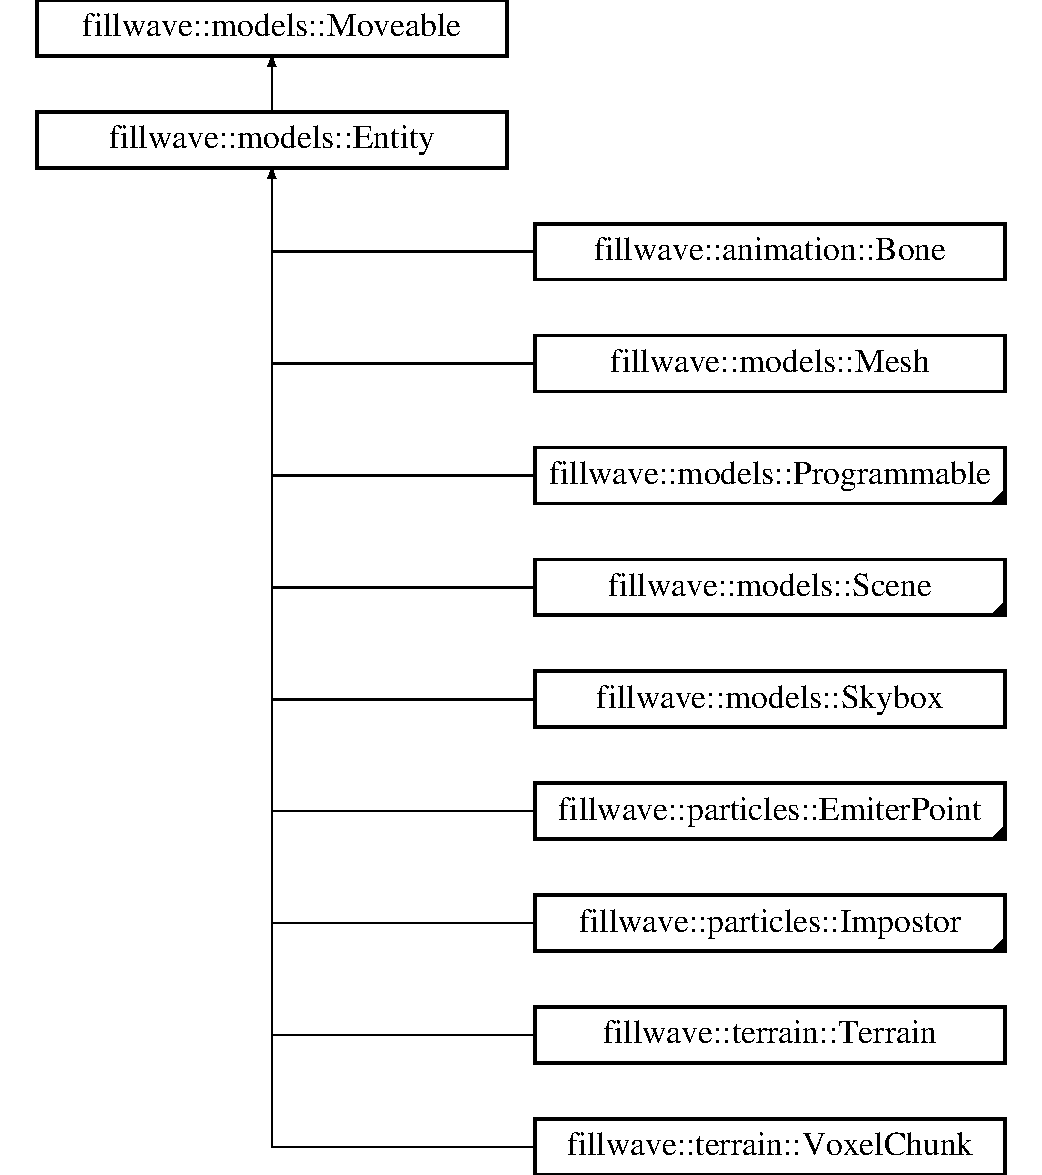
\includegraphics[height=11.000000cm]{classfillwave_1_1models_1_1Entity}
\end{center}
\end{figure}
\subsection*{Public Member Functions}
\begin{DoxyCompactItemize}
\item 
\hypertarget{classfillwave_1_1models_1_1Entity_aeb0600d09ee5d57db3f4c76984ebea2c}{}{\bfseries Entity} (glm\+::vec3 translation=glm\+::vec3(0.\+0), glm\+::quat orientation=glm\+::quat(1.\+0, 0.\+0, 0.\+0, 0.\+0))\label{classfillwave_1_1models_1_1Entity_aeb0600d09ee5d57db3f4c76984ebea2c}

\item 
\hypertarget{classfillwave_1_1models_1_1Entity_a377e85bb6666e808004471721232b7e4}{}void {\bfseries attach} (p\+Entity child)\label{classfillwave_1_1models_1_1Entity_a377e85bb6666e808004471721232b7e4}

\item 
\hypertarget{classfillwave_1_1models_1_1Entity_a8f3d3d1291491ae61930e7159634ccb0}{}void {\bfseries detach} (p\+Entity child)\label{classfillwave_1_1models_1_1Entity_a8f3d3d1291491ae61930e7159634ccb0}

\item 
\hypertarget{classfillwave_1_1models_1_1Entity_ad63db6ab433c1bfba2ec8222a15dd956}{}void {\bfseries on\+Detached} ()\label{classfillwave_1_1models_1_1Entity_ad63db6ab433c1bfba2ec8222a15dd956}

\item 
\hypertarget{classfillwave_1_1models_1_1Entity_af4a59792cf177d095aef718881ede8aa}{}void {\bfseries on\+Attached} (\hyperlink{classfillwave_1_1models_1_1Entity}{Entity} $\ast$parent)\label{classfillwave_1_1models_1_1Entity_af4a59792cf177d095aef718881ede8aa}

\item 
\hypertarget{classfillwave_1_1models_1_1Entity_ab9892968cd70d1abfb8d36660a71865a}{}virtual void {\bfseries draw} (\hyperlink{classfillwave_1_1space_1_1Camera}{space\+::\+Camera} \&camera)\label{classfillwave_1_1models_1_1Entity_ab9892968cd70d1abfb8d36660a71865a}

\item 
\hypertarget{classfillwave_1_1models_1_1Entity_a37b5d9b3aaa361aaf99c4649023314f7}{}virtual void {\bfseries draw\+D\+R} (\hyperlink{classfillwave_1_1space_1_1Camera}{space\+::\+Camera} \&camera)\label{classfillwave_1_1models_1_1Entity_a37b5d9b3aaa361aaf99c4649023314f7}

\item 
\hypertarget{classfillwave_1_1models_1_1Entity_ad49b41494b75d856d60dafcce88737ec}{}virtual void {\bfseries draw\+Depth} (\hyperlink{classfillwave_1_1space_1_1Camera}{space\+::\+Camera} \&camera)\label{classfillwave_1_1models_1_1Entity_ad49b41494b75d856d60dafcce88737ec}

\item 
\hypertarget{classfillwave_1_1models_1_1Entity_a583178291e394e22ba0e5f0c04229f30}{}virtual void {\bfseries draw\+Depth\+Color} (\hyperlink{classfillwave_1_1space_1_1Camera}{space\+::\+Camera} \&camera, glm\+::vec3 \&position)\label{classfillwave_1_1models_1_1Entity_a583178291e394e22ba0e5f0c04229f30}

\item 
\hypertarget{classfillwave_1_1models_1_1Entity_a29287c866cb76e14f64ae2b5e2aabf28}{}virtual void {\bfseries draw\+A\+O\+G} (\hyperlink{classfillwave_1_1space_1_1Camera}{space\+::\+Camera} \&camera)\label{classfillwave_1_1models_1_1Entity_a29287c866cb76e14f64ae2b5e2aabf28}

\item 
\hypertarget{classfillwave_1_1models_1_1Entity_ac350b688827706bd41598911d2658ddf}{}virtual void {\bfseries draw\+A\+O\+C} (\hyperlink{classfillwave_1_1space_1_1Camera}{space\+::\+Camera} \&camera)\label{classfillwave_1_1models_1_1Entity_ac350b688827706bd41598911d2658ddf}

\item 
\hypertarget{classfillwave_1_1models_1_1Entity_a226154ecde4890558d7153f8e71e00a3}{}virtual void {\bfseries draw\+Occlusion\+Box} (\hyperlink{classfillwave_1_1space_1_1Camera}{space\+::\+Camera} \&camera)\label{classfillwave_1_1models_1_1Entity_a226154ecde4890558d7153f8e71e00a3}

\item 
\hypertarget{classfillwave_1_1models_1_1Entity_af5de8adfe4da7787823c18a80d20d6a9}{}G\+Lboolean {\bfseries is\+P\+S\+C} ()\label{classfillwave_1_1models_1_1Entity_af5de8adfe4da7787823c18a80d20d6a9}

\item 
\hypertarget{classfillwave_1_1models_1_1Entity_ae54bed7959446c88541b0aa3e4956fe8}{}G\+Lboolean {\bfseries is\+P\+S\+R} ()\label{classfillwave_1_1models_1_1Entity_ae54bed7959446c88541b0aa3e4956fe8}

\item 
\hypertarget{classfillwave_1_1models_1_1Entity_a1b0402696711a20db58c65cfe6f5b23f}{}void {\bfseries handle\+Hierarchy\+Event} (\hyperlink{classfillwave_1_1actions_1_1EventType}{actions\+::\+Event\+Type} $\ast$event)\label{classfillwave_1_1models_1_1Entity_a1b0402696711a20db58c65cfe6f5b23f}

\item 
\hypertarget{classfillwave_1_1models_1_1Entity_ada0f6dd45517daf49c0a83b4b844b70c}{}void {\bfseries handle\+Private\+Event} (\hyperlink{classfillwave_1_1actions_1_1EventType}{actions\+::\+Event\+Type} $\ast$event)\label{classfillwave_1_1models_1_1Entity_ada0f6dd45517daf49c0a83b4b844b70c}

\item 
\hypertarget{classfillwave_1_1models_1_1Entity_a0b4448ce50783fe805c1c2d53e02d8de}{}glm\+::mat4 {\bfseries get\+Transformation} ()\label{classfillwave_1_1models_1_1Entity_a0b4448ce50783fe805c1c2d53e02d8de}

\item 
\hypertarget{classfillwave_1_1models_1_1Entity_ab3b721b4d7e31c4427e875be54138fc0}{}void {\bfseries set\+Transformation} (glm\+::mat4 model\+Matrix)\label{classfillwave_1_1models_1_1Entity_ab3b721b4d7e31c4427e875be54138fc0}

\item 
\hypertarget{classfillwave_1_1models_1_1Entity_a63d67b1d8a5d5c232c1a40db39d263e7}{}void {\bfseries attach\+Hierarchy\+Callback} (\hyperlink{classfillwave_1_1actions_1_1ItemCallback}{actions\+::\+Item\+Callback} $\ast$callback)\label{classfillwave_1_1models_1_1Entity_a63d67b1d8a5d5c232c1a40db39d263e7}

\item 
\hypertarget{classfillwave_1_1models_1_1Entity_a2f09305545cb13a242df3a2de32798d8}{}void {\bfseries attach\+Private\+Callback} (\hyperlink{classfillwave_1_1actions_1_1ItemCallback}{actions\+::\+Item\+Callback} $\ast$callback)\label{classfillwave_1_1models_1_1Entity_a2f09305545cb13a242df3a2de32798d8}

\item 
\hypertarget{classfillwave_1_1models_1_1Entity_a880349eb2ec5124b57ef779a572748a7}{}void {\bfseries detach\+Hierarchy\+Callback} (\hyperlink{classfillwave_1_1actions_1_1ItemCallback}{actions\+::\+Item\+Callback} $\ast$callback)\label{classfillwave_1_1models_1_1Entity_a880349eb2ec5124b57ef779a572748a7}

\item 
\hypertarget{classfillwave_1_1models_1_1Entity_a3ce284d090d050331889fd46af82152e}{}void {\bfseries detach\+Private\+Callback} (\hyperlink{classfillwave_1_1actions_1_1ItemCallback}{actions\+::\+Item\+Callback} $\ast$callback)\label{classfillwave_1_1models_1_1Entity_a3ce284d090d050331889fd46af82152e}

\item 
\hypertarget{classfillwave_1_1models_1_1Entity_aef0790065a393c9cece4a6ab3f997ce9}{}void {\bfseries update\+Matrix\+Tree} ()\label{classfillwave_1_1models_1_1Entity_aef0790065a393c9cece4a6ab3f997ce9}

\item 
\hypertarget{classfillwave_1_1models_1_1Entity_ae3ecab5cfb2400faa1cb76de8e252d4d}{}void {\bfseries update\+Parent\+Matrix} (glm\+::mat4 \&parent)\label{classfillwave_1_1models_1_1Entity_ae3ecab5cfb2400faa1cb76de8e252d4d}

\item 
\hypertarget{classfillwave_1_1models_1_1Entity_a19a6bc95be9e7fdb697762295b621f5a}{}void {\bfseries update\+Parent\+Rotation} (glm\+::quat \&rotation)\label{classfillwave_1_1models_1_1Entity_a19a6bc95be9e7fdb697762295b621f5a}

\item 
\hypertarget{classfillwave_1_1models_1_1Entity_a4ba3e493ac6cdea186887121f934516c}{}glm\+::mat4 {\bfseries get\+Parent\+Matrix} ()\label{classfillwave_1_1models_1_1Entity_a4ba3e493ac6cdea186887121f934516c}

\item 
\hypertarget{classfillwave_1_1models_1_1Entity_a93a01975a6bddd1d551d8f27e09d887d}{}glm\+::quat {\bfseries get\+Parent\+Rotation} ()\label{classfillwave_1_1models_1_1Entity_a93a01975a6bddd1d551d8f27e09d887d}

\item 
\hypertarget{classfillwave_1_1models_1_1Entity_af5aee0aab5f39f36c13964acc449ecac}{}void {\bfseries pick} (glm\+::vec3 color)\label{classfillwave_1_1models_1_1Entity_af5aee0aab5f39f36c13964acc449ecac}

\item 
\hypertarget{classfillwave_1_1models_1_1Entity_a03671255f61af07591bdd4cb6245bb18}{}void {\bfseries unpick} ()\label{classfillwave_1_1models_1_1Entity_a03671255f61af07591bdd4cb6245bb18}

\item 
\hypertarget{classfillwave_1_1models_1_1Entity_a4983228d7de32c49f0625ebe7deef4bb}{}G\+Lboolean {\bfseries is\+Pickable} ()\label{classfillwave_1_1models_1_1Entity_a4983228d7de32c49f0625ebe7deef4bb}

\item 
\hypertarget{classfillwave_1_1models_1_1Entity_a82afce21fa642d38fb236cc2630b9925}{}glm\+::vec3 {\bfseries get\+Pickable\+Color} ()\label{classfillwave_1_1models_1_1Entity_a82afce21fa642d38fb236cc2630b9925}

\item 
\hypertarget{classfillwave_1_1models_1_1Entity_ad982b344b6dda2451856c6c228540b09}{}virtual void {\bfseries on\+Picked} ()\label{classfillwave_1_1models_1_1Entity_ad982b344b6dda2451856c6c228540b09}

\item 
\hypertarget{classfillwave_1_1models_1_1Entity_acf69269a84cbd349a5ae02e969791bc4}{}virtual void {\bfseries on\+Unpicked} ()\label{classfillwave_1_1models_1_1Entity_acf69269a84cbd349a5ae02e969791bc4}

\item 
\hypertarget{classfillwave_1_1models_1_1Entity_aed04b4ea3b5336635456a1fe2ec43692}{}virtual void {\bfseries draw\+Picking} (\hyperlink{classfillwave_1_1space_1_1Camera}{space\+::\+Camera} \&camera)\label{classfillwave_1_1models_1_1Entity_aed04b4ea3b5336635456a1fe2ec43692}

\item 
\hypertarget{classfillwave_1_1models_1_1Entity_a81b24880a8c14d33ef8be8fa39a6adfd}{}void {\bfseries set\+External\+Refresh} (G\+Lboolean state)\label{classfillwave_1_1models_1_1Entity_a81b24880a8c14d33ef8be8fa39a6adfd}

\item 
\hypertarget{classfillwave_1_1models_1_1Entity_a96e05e30df7fc44d2da57c97659926a5}{}G\+Lboolean {\bfseries is\+External\+Refresh} ()\label{classfillwave_1_1models_1_1Entity_a96e05e30df7fc44d2da57c97659926a5}

\item 
\hypertarget{classfillwave_1_1models_1_1Entity_a0f551d5bf0b35552c81f2e336d615779}{}void {\bfseries set\+External\+Refresh} ()\label{classfillwave_1_1models_1_1Entity_a0f551d5bf0b35552c81f2e336d615779}

\item 
\hypertarget{classfillwave_1_1models_1_1Entity_a712b5db092813f297fe5a4d73394db02}{}virtual void {\bfseries log} ()\label{classfillwave_1_1models_1_1Entity_a712b5db092813f297fe5a4d73394db02}

\end{DoxyCompactItemize}
\subsection*{Protected Attributes}
\begin{DoxyCompactItemize}
\item 
\hypertarget{classfillwave_1_1models_1_1Entity_ae4417f42009ce2d77bac972510f4ddc9}{}glm\+::quat {\bfseries m\+Parent\+Rotation}\label{classfillwave_1_1models_1_1Entity_ae4417f42009ce2d77bac972510f4ddc9}

\item 
\hypertarget{classfillwave_1_1models_1_1Entity_a5bed161efeaa6c9ba49e8c24659a61d9}{}glm\+::mat4 {\bfseries m\+Parent\+Matrix}\label{classfillwave_1_1models_1_1Entity_a5bed161efeaa6c9ba49e8c24659a61d9}

\item 
\hypertarget{classfillwave_1_1models_1_1Entity_a80a2e5b0bc1695a8075b4a0e216835f5}{}glm\+::mat4 {\bfseries m\+Transformation}\label{classfillwave_1_1models_1_1Entity_a80a2e5b0bc1695a8075b4a0e216835f5}

\item 
\hypertarget{classfillwave_1_1models_1_1Entity_a0490ceec51cf87359298fcb77c836baf}{}G\+Lboolean {\bfseries m\+Parent\+Refresh}\label{classfillwave_1_1models_1_1Entity_a0490ceec51cf87359298fcb77c836baf}

\item 
\hypertarget{classfillwave_1_1models_1_1Entity_af7f12c3d43c8defc4cd737387117cc89}{}std\+::vector$<$ p\+Entity $>$ {\bfseries m\+Children}\label{classfillwave_1_1models_1_1Entity_af7f12c3d43c8defc4cd737387117cc89}

\item 
\hypertarget{classfillwave_1_1models_1_1Entity_a9a0eceac5f40cc6f462ab7651cd725b4}{}G\+Lboolean {\bfseries m\+Children\+Propagate\+Event}\label{classfillwave_1_1models_1_1Entity_a9a0eceac5f40cc6f462ab7651cd725b4}

\item 
\hypertarget{classfillwave_1_1models_1_1Entity_ae4f7b1d6eef02eee01addc85be9a6411}{}std\+::vector$<$ \hyperlink{classfillwave_1_1actions_1_1ItemCallback}{actions\+::\+Item\+Callback} $\ast$ $>$ {\bfseries m\+Callbacks\+Hierarchy}\label{classfillwave_1_1models_1_1Entity_ae4f7b1d6eef02eee01addc85be9a6411}

\item 
\hypertarget{classfillwave_1_1models_1_1Entity_abd1895e1cfe2ba0349c8023e2970dc8d}{}std\+::vector$<$ \hyperlink{classfillwave_1_1actions_1_1ItemCallback}{actions\+::\+Item\+Callback} $\ast$ $>$ {\bfseries m\+Callbacks\+Private}\label{classfillwave_1_1models_1_1Entity_abd1895e1cfe2ba0349c8023e2970dc8d}

\item 
\hypertarget{classfillwave_1_1models_1_1Entity_a774a4749e0f234ce0c6d064b48500530}{}G\+Lboolean {\bfseries m\+P\+S\+C}\label{classfillwave_1_1models_1_1Entity_a774a4749e0f234ce0c6d064b48500530}

\item 
\hypertarget{classfillwave_1_1models_1_1Entity_a52025db4b7358d48995069c91ccd31a0}{}G\+Lboolean {\bfseries m\+P\+S\+R}\label{classfillwave_1_1models_1_1Entity_a52025db4b7358d48995069c91ccd31a0}

\end{DoxyCompactItemize}


\subsection{Detailed Description}
Base for all \hyperlink{classfillwave_1_1models_1_1Scene}{Scene} nodes. 

The documentation for this class was generated from the following file\+:\begin{DoxyCompactItemize}
\item 
/home/filip/\+Projects/fillwave/inc/fillwave/models/Entity.\+h\end{DoxyCompactItemize}

\hypertarget{classfillwave_1_1actions_1_1Event}{}\section{fillwave\+:\+:actions\+:\+:Event$<$ T $>$ Class Template Reference}
\label{classfillwave_1_1actions_1_1Event}\index{fillwave\+::actions\+::\+Event$<$ T $>$@{fillwave\+::actions\+::\+Event$<$ T $>$}}


Template for all events.  




{\ttfamily \#include $<$Event.\+h$>$}

Inheritance diagram for fillwave\+:\+:actions\+:\+:Event$<$ T $>$\+:\begin{figure}[H]
\begin{center}
\leavevmode
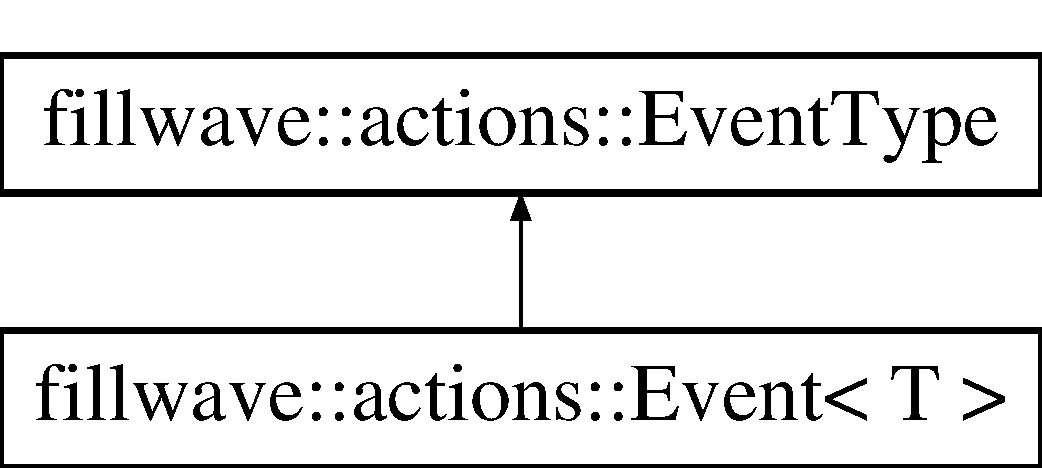
\includegraphics[height=2.000000cm]{classfillwave_1_1actions_1_1Event}
\end{center}
\end{figure}
\subsection*{Public Member Functions}
\begin{DoxyCompactItemize}
\item 
\hypertarget{classfillwave_1_1actions_1_1Event_a6169d5fd6bfb41c60831b91294504b05}{}{\bfseries Event} (T data)\label{classfillwave_1_1actions_1_1Event_a6169d5fd6bfb41c60831b91294504b05}

\end{DoxyCompactItemize}
\subsection*{Static Public Member Functions}
\begin{DoxyCompactItemize}
\item 
\hypertarget{classfillwave_1_1actions_1_1Event_a817aeb52af71ead58bd052be5ffae3ee}{}static T {\bfseries get\+Data} (\hyperlink{classfillwave_1_1actions_1_1EventType}{Event\+Type} $\ast$event\+Type)\label{classfillwave_1_1actions_1_1Event_a817aeb52af71ead58bd052be5ffae3ee}

\item 
\hypertarget{classfillwave_1_1actions_1_1Event_aab62154289dcbab43daa2fe26985ab23}{}static \hyperlink{classfillwave_1_1actions_1_1Event}{Event}$<$ T $>$ $\ast$ {\bfseries get\+Event} (\hyperlink{classfillwave_1_1actions_1_1EventType}{Event\+Type} $\ast$event\+Type)\label{classfillwave_1_1actions_1_1Event_aab62154289dcbab43daa2fe26985ab23}

\end{DoxyCompactItemize}


\subsection{Detailed Description}
\subsubsection*{template$<$class T$>$class fillwave\+::actions\+::\+Event$<$ T $>$}

Template for all events. 

This class needs to be specialized by the certain type of event You want to be carried. 

The documentation for this class was generated from the following file\+:\begin{DoxyCompactItemize}
\item 
/home/filip/\+Projects/fillwave/inc/fillwave/actions/Event.\+h\end{DoxyCompactItemize}

\hypertarget{classfillwave_1_1actions_1_1EventType}{}\section{fillwave\+:\+:actions\+:\+:Event\+Type Class Reference}
\label{classfillwave_1_1actions_1_1EventType}\index{fillwave\+::actions\+::\+Event\+Type@{fillwave\+::actions\+::\+Event\+Type}}


Base class for all events. This class needs only the event type (literally -\/ an enumerator) to initialize. \hyperlink{classfillwave_1_1actions_1_1Event}{Event} type defines by which callback the event will be handled.  




{\ttfamily \#include $<$Event\+Type.\+h$>$}

Inheritance diagram for fillwave\+:\+:actions\+:\+:Event\+Type\+:\begin{figure}[H]
\begin{center}
\leavevmode
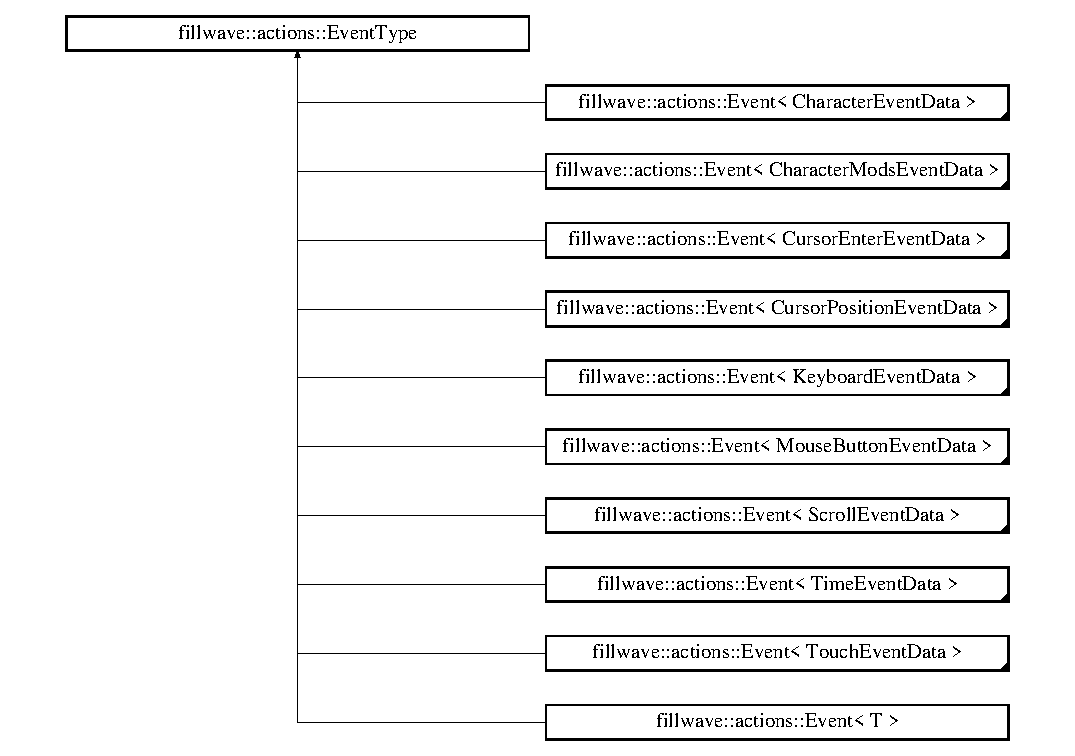
\includegraphics[height=9.716088cm]{classfillwave_1_1actions_1_1EventType}
\end{center}
\end{figure}
\subsection*{Public Member Functions}
\begin{DoxyCompactItemize}
\item 
\hypertarget{classfillwave_1_1actions_1_1EventType_a221bb02b1f5c6e04695707ba47abd61b}{}{\bfseries Event\+Type} (e\+Event\+Type type)\label{classfillwave_1_1actions_1_1EventType_a221bb02b1f5c6e04695707ba47abd61b}

\item 
\hypertarget{classfillwave_1_1actions_1_1EventType_adf6612d2c6a3edd17f1cdd313355d62c}{}e\+Event\+Type {\bfseries get\+Type} ()\label{classfillwave_1_1actions_1_1EventType_adf6612d2c6a3edd17f1cdd313355d62c}

\end{DoxyCompactItemize}


\subsection{Detailed Description}
Base class for all events. This class needs only the event type (literally -\/ an enumerator) to initialize. \hyperlink{classfillwave_1_1actions_1_1Event}{Event} type defines by which callback the event will be handled. 

The documentation for this class was generated from the following file\+:\begin{DoxyCompactItemize}
\item 
/home/filip/\+Projects/fillwave/inc/fillwave/actions/Event\+Type.\+h\end{DoxyCompactItemize}

\hypertarget{structfillwave_1_1core_1_1FaceBasic}{}\section{fillwave\+:\+:core\+:\+:Face\+Basic Struct Reference}
\label{structfillwave_1_1core_1_1FaceBasic}\index{fillwave\+::core\+::\+Face\+Basic@{fillwave\+::core\+::\+Face\+Basic}}


Stores the face data for geometry built on Vertex Basic.  




{\ttfamily \#include $<$Vertex\+Buffer\+Basic.\+h$>$}

\subsection*{Public Attributes}
\begin{DoxyCompactItemize}
\item 
\hypertarget{structfillwave_1_1core_1_1FaceBasic_acba94f7799b27b0e0ce319af3d706e15}{}\hyperlink{structfillwave_1_1core_1_1VertexBasic}{core\+::\+Vertex\+Basic} {\bfseries vertices} \mbox{[}3\mbox{]}\label{structfillwave_1_1core_1_1FaceBasic_acba94f7799b27b0e0ce319af3d706e15}

\end{DoxyCompactItemize}


\subsection{Detailed Description}
Stores the face data for geometry built on Vertex Basic. 

The documentation for this struct was generated from the following file\+:\begin{DoxyCompactItemize}
\item 
/home/filip/\+Projects/fillwave/inc/fillwave/core/buffers/Vertex\+Buffer\+Basic.\+h\end{DoxyCompactItemize}

\hypertarget{classfillwave_1_1core_1_1Fence}{}\section{fillwave\+:\+:core\+:\+:Fence Class Reference}
\label{classfillwave_1_1core_1_1Fence}\index{fillwave\+::core\+::\+Fence@{fillwave\+::core\+::\+Fence}}


Sets a fence for a gpu to wait.  




{\ttfamily \#include $<$Fence.\+h$>$}

\subsection*{Public Member Functions}
\begin{DoxyCompactItemize}
\item 
\hypertarget{classfillwave_1_1core_1_1Fence_a0fc91f6b1c08d750e63fbe1c09c3ab5b}{}{\bfseries Fence} (G\+Lenum target=G\+L\+\_\+\+S\+Y\+N\+C\+\_\+\+G\+P\+U\+\_\+\+C\+O\+M\+M\+A\+N\+D\+S\+\_\+\+C\+O\+M\+P\+L\+E\+T\+E)\label{classfillwave_1_1core_1_1Fence_a0fc91f6b1c08d750e63fbe1c09c3ab5b}

\item 
\hypertarget{classfillwave_1_1core_1_1Fence_a852e254cea189d2275a035bfc1c73e17}{}void {\bfseries wait} (unsigned long long timeout\+Specifier=G\+L\+\_\+\+T\+I\+M\+E\+O\+U\+T\+\_\+\+I\+G\+N\+O\+R\+E\+D)\label{classfillwave_1_1core_1_1Fence_a852e254cea189d2275a035bfc1c73e17}

\end{DoxyCompactItemize}


\subsection{Detailed Description}
Sets a fence for a gpu to wait. 

The documentation for this class was generated from the following file\+:\begin{DoxyCompactItemize}
\item 
/home/filip/\+Projects/fillwave/inc/fillwave/core/pipeline/Fence.\+h\end{DoxyCompactItemize}

\hypertarget{classfillwave_1_1loader_1_1FileLoader}{}\section{fillwave\+:\+:loader\+:\+:File\+Loader Class Reference}
\label{classfillwave_1_1loader_1_1FileLoader}\index{fillwave\+::loader\+::\+File\+Loader@{fillwave\+::loader\+::\+File\+Loader}}


Loads files.  




{\ttfamily \#include $<$File\+Loader.\+h$>$}

\subsection*{Public Member Functions}
\begin{DoxyCompactItemize}
\item 
\hypertarget{classfillwave_1_1loader_1_1FileLoader_a53006e2e7d5cc39317928a0065992e2d}{}{\bfseries File\+Loader} (const std\+::string \&root\+Path)\label{classfillwave_1_1loader_1_1FileLoader_a53006e2e7d5cc39317928a0065992e2d}

\item 
\hypertarget{classfillwave_1_1loader_1_1FileLoader_a867d0d51e34560ccc1c48e2a546260f9}{}std\+::string {\bfseries get\+Root\+Path} (std\+::string file\+Path=\char`\"{}\char`\"{})\label{classfillwave_1_1loader_1_1FileLoader_a867d0d51e34560ccc1c48e2a546260f9}

\end{DoxyCompactItemize}


\subsection{Detailed Description}
Loads files. 

The documentation for this class was generated from the following file\+:\begin{DoxyCompactItemize}
\item 
/home/filip/\+Projects/fillwave/inc/fillwave/loaders/File\+Loader.\+h\end{DoxyCompactItemize}

\hypertarget{classfillwave_1_1common_1_1Finishable}{}\section{fillwave\+:\+:common\+:\+:Finishable Class Reference}
\label{classfillwave_1_1common_1_1Finishable}\index{fillwave\+::common\+::\+Finishable@{fillwave\+::common\+::\+Finishable}}


Base for every finishable callback.  




{\ttfamily \#include $<$Finishable.\+h$>$}

Inheritance diagram for fillwave\+:\+:common\+:\+:Finishable\+:\begin{figure}[H]
\begin{center}
\leavevmode
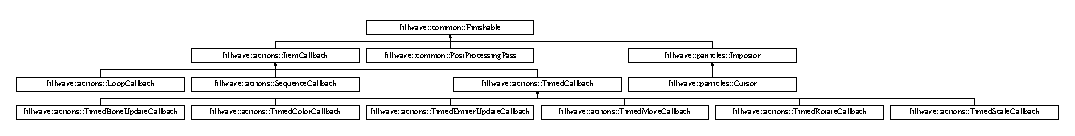
\includegraphics[height=1.377614cm]{classfillwave_1_1common_1_1Finishable}
\end{center}
\end{figure}
\subsection*{Public Member Functions}
\begin{DoxyCompactItemize}
\item 
\hypertarget{classfillwave_1_1common_1_1Finishable_a4e82504fc8af19c480170ec836d0b400}{}{\bfseries Finishable} (float time\+To\+Finish)\label{classfillwave_1_1common_1_1Finishable_a4e82504fc8af19c480170ec836d0b400}

\item 
\hypertarget{classfillwave_1_1common_1_1Finishable_aecc37f0d5ed793ab1f446a6d11e8b29d}{}void {\bfseries check\+Time} (float time\+Passed)\label{classfillwave_1_1common_1_1Finishable_aecc37f0d5ed793ab1f446a6d11e8b29d}

\item 
\hypertarget{classfillwave_1_1common_1_1Finishable_a75db5fbcb2651c9a1a05a8ebf3978038}{}float {\bfseries get\+Percentage\+Done} () const \label{classfillwave_1_1common_1_1Finishable_a75db5fbcb2651c9a1a05a8ebf3978038}

\item 
\hypertarget{classfillwave_1_1common_1_1Finishable_a1b5ad3219468ddaa449f3330b2aa660c}{}void {\bfseries finish} ()\label{classfillwave_1_1common_1_1Finishable_a1b5ad3219468ddaa449f3330b2aa660c}

\item 
\hypertarget{classfillwave_1_1common_1_1Finishable_a79a1f23e168c734489973ce8cf2c373b}{}void {\bfseries reset} ()\label{classfillwave_1_1common_1_1Finishable_a79a1f23e168c734489973ce8cf2c373b}

\item 
\hypertarget{classfillwave_1_1common_1_1Finishable_a14fdfaf4574f50dd27723d1ea50a3276}{}bool {\bfseries is\+Finished} () const \label{classfillwave_1_1common_1_1Finishable_a14fdfaf4574f50dd27723d1ea50a3276}

\end{DoxyCompactItemize}
\subsection*{Protected Attributes}
\begin{DoxyCompactItemize}
\item 
\hypertarget{classfillwave_1_1common_1_1Finishable_a6ff5cf040384c89ca596387efde649a7}{}float {\bfseries m\+Percentage\+Done}\label{classfillwave_1_1common_1_1Finishable_a6ff5cf040384c89ca596387efde649a7}

\item 
\hypertarget{classfillwave_1_1common_1_1Finishable_a3ae8d9913828e82d5762ebe88942c198}{}float {\bfseries m\+Time\+To\+Finish}\label{classfillwave_1_1common_1_1Finishable_a3ae8d9913828e82d5762ebe88942c198}

\item 
\hypertarget{classfillwave_1_1common_1_1Finishable_a7512122b86184a2d4f885816abbbbebc}{}float {\bfseries m\+Time\+Passed}\label{classfillwave_1_1common_1_1Finishable_a7512122b86184a2d4f885816abbbbebc}

\item 
\hypertarget{classfillwave_1_1common_1_1Finishable_ab78ce1f4ef07a832654bca45a9bf2650}{}bool {\bfseries m\+Finished}\label{classfillwave_1_1common_1_1Finishable_ab78ce1f4ef07a832654bca45a9bf2650}

\end{DoxyCompactItemize}


\subsection{Detailed Description}
Base for every finishable callback. 

The documentation for this class was generated from the following file\+:\begin{DoxyCompactItemize}
\item 
/home/filip/\+Projects/fillwave/inc/fillwave/common/Finishable.\+h\end{DoxyCompactItemize}

\hypertarget{classfillwave_1_1effects_1_1Fog}{}\section{fillwave\+:\+:effects\+:\+:Fog Class Reference}
\label{classfillwave_1_1effects_1_1Fog}\index{fillwave\+::effects\+::\+Fog@{fillwave\+::effects\+::\+Fog}}


\hyperlink{classfillwave_1_1effects_1_1Effect}{Effect} to create a fog.  




{\ttfamily \#include $<$Fog.\+h$>$}

Inheritance diagram for fillwave\+:\+:effects\+:\+:Fog\+:\begin{figure}[H]
\begin{center}
\leavevmode
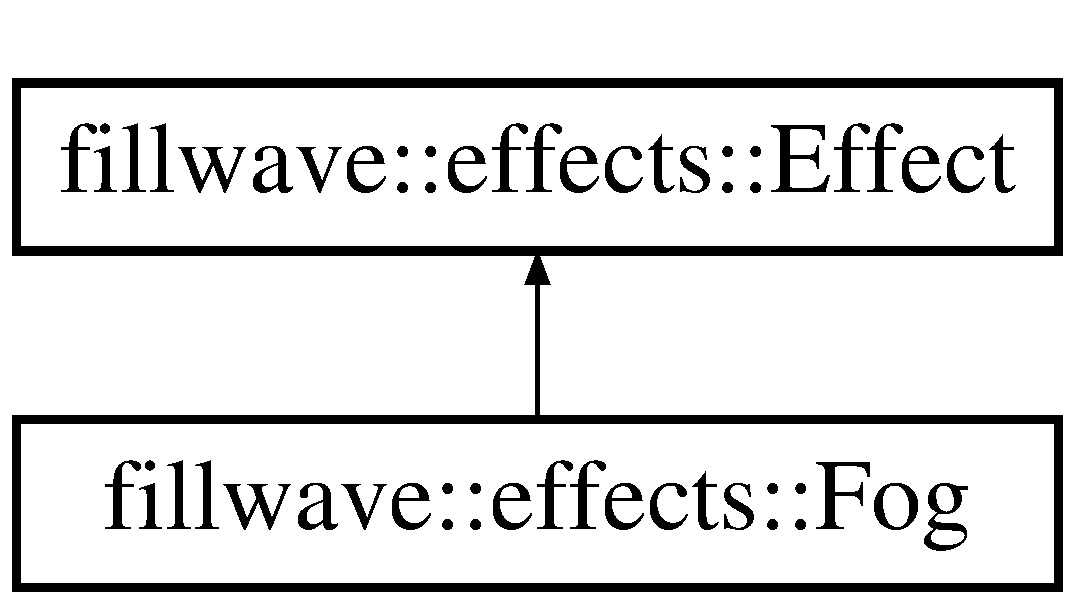
\includegraphics[height=2.000000cm]{classfillwave_1_1effects_1_1Fog}
\end{center}
\end{figure}
\subsection*{Public Member Functions}
\begin{DoxyCompactItemize}
\item 
\hypertarget{classfillwave_1_1effects_1_1Fog_abb5ae920df6298b4336a2ed4e702a955}{}glm\+::vec3 {\bfseries get\+Colour} ()\label{classfillwave_1_1effects_1_1Fog_abb5ae920df6298b4336a2ed4e702a955}

\item 
\hypertarget{classfillwave_1_1effects_1_1Fog_a26f0b406b8e6b9629fc9e9e3b9bb625b}{}G\+Lfloat {\bfseries get\+Near\+Distance} ()\label{classfillwave_1_1effects_1_1Fog_a26f0b406b8e6b9629fc9e9e3b9bb625b}

\item 
\hypertarget{classfillwave_1_1effects_1_1Fog_a8b74e06482d55497ee8af7a7a728e534}{}G\+Lfloat {\bfseries get\+Far\+Distance} ()\label{classfillwave_1_1effects_1_1Fog_a8b74e06482d55497ee8af7a7a728e534}

\item 
\hypertarget{classfillwave_1_1effects_1_1Fog_a79ae82e784fcbbc60886ecd052d5acea}{}void {\bfseries set\+Colour} (glm\+::vec3 colour)\label{classfillwave_1_1effects_1_1Fog_a79ae82e784fcbbc60886ecd052d5acea}

\item 
\hypertarget{classfillwave_1_1effects_1_1Fog_acabf149d0aee3fcbb38783db783b5a8b}{}void {\bfseries set\+Near\+Distance} (G\+Lfloat near)\label{classfillwave_1_1effects_1_1Fog_acabf149d0aee3fcbb38783db783b5a8b}

\item 
\hypertarget{classfillwave_1_1effects_1_1Fog_a635e0de9761fd2cdb1847534cef6f6f9}{}void {\bfseries set\+Far\+Distance} (G\+Lfloat far)\label{classfillwave_1_1effects_1_1Fog_a635e0de9761fd2cdb1847534cef6f6f9}

\item 
\hypertarget{classfillwave_1_1effects_1_1Fog_aa5535dd253110c88f9e3be21095ca4e4}{}{\bfseries Fog} (glm\+::vec3 colour=glm\+::vec3(0.\+1, 0.\+1, 0.\+1), G\+Lfloat near=0.\+1, G\+Lfloat far=20.\+0f)\label{classfillwave_1_1effects_1_1Fog_aa5535dd253110c88f9e3be21095ca4e4}

\item 
void \hyperlink{classfillwave_1_1effects_1_1Fog_a943f060680f000663eba8b2c93398ee8}{pre\+Draw\+Action} (\hyperlink{classfillwave_1_1core_1_1Program}{core\+::\+Program} $\ast$program)
\begin{DoxyCompactList}\small\item\em virtual\+: defines action to be done just before the draw. \end{DoxyCompactList}\item 
void \hyperlink{classfillwave_1_1effects_1_1Fog_a2a625835d139fb614a5325acba7604fc}{post\+Draw\+Action} (\hyperlink{classfillwave_1_1core_1_1Program}{core\+::\+Program} $\ast$program)
\begin{DoxyCompactList}\small\item\em virtual\+: defines action to be done just after the draw. \end{DoxyCompactList}\item 
void \hyperlink{classfillwave_1_1effects_1_1Fog_a2b5eb2628c9db559446619db744ebed5}{stop\+Action} (\hyperlink{classfillwave_1_1core_1_1Program}{core\+::\+Program} $\ast$program)
\begin{DoxyCompactList}\small\item\em virtual\+: defines action to be done when the effect is stopped. \end{DoxyCompactList}\item 
void \hyperlink{classfillwave_1_1effects_1_1Fog_a8a7c4a0fb2f5cb95873d2b827354a4f8}{start\+Action} (\hyperlink{classfillwave_1_1core_1_1Program}{core\+::\+Program} $\ast$program)
\begin{DoxyCompactList}\small\item\em virtual\+: defines action to be done when the effect is started. \end{DoxyCompactList}\end{DoxyCompactItemize}


\subsection{Detailed Description}
\hyperlink{classfillwave_1_1effects_1_1Effect}{Effect} to create a fog. 

\subsection{Member Function Documentation}
\hypertarget{classfillwave_1_1effects_1_1Fog_a2a625835d139fb614a5325acba7604fc}{}\index{fillwave\+::effects\+::\+Fog@{fillwave\+::effects\+::\+Fog}!post\+Draw\+Action@{post\+Draw\+Action}}
\index{post\+Draw\+Action@{post\+Draw\+Action}!fillwave\+::effects\+::\+Fog@{fillwave\+::effects\+::\+Fog}}
\subsubsection[{post\+Draw\+Action}]{\setlength{\rightskip}{0pt plus 5cm}void fillwave\+::effects\+::\+Fog\+::post\+Draw\+Action (
\begin{DoxyParamCaption}
\item[{{\bf core\+::\+Program} $\ast$}]{program}
\end{DoxyParamCaption}
)\hspace{0.3cm}{\ttfamily [virtual]}}\label{classfillwave_1_1effects_1_1Fog_a2a625835d139fb614a5325acba7604fc}


virtual\+: defines action to be done just after the draw. 

post\+Draw\+Action 

Implements \hyperlink{classfillwave_1_1effects_1_1Effect_ae01123633990402e11226c4d9a2dce1b}{fillwave\+::effects\+::\+Effect}.

\hypertarget{classfillwave_1_1effects_1_1Fog_a943f060680f000663eba8b2c93398ee8}{}\index{fillwave\+::effects\+::\+Fog@{fillwave\+::effects\+::\+Fog}!pre\+Draw\+Action@{pre\+Draw\+Action}}
\index{pre\+Draw\+Action@{pre\+Draw\+Action}!fillwave\+::effects\+::\+Fog@{fillwave\+::effects\+::\+Fog}}
\subsubsection[{pre\+Draw\+Action}]{\setlength{\rightskip}{0pt plus 5cm}void fillwave\+::effects\+::\+Fog\+::pre\+Draw\+Action (
\begin{DoxyParamCaption}
\item[{{\bf core\+::\+Program} $\ast$}]{program}
\end{DoxyParamCaption}
)\hspace{0.3cm}{\ttfamily [virtual]}}\label{classfillwave_1_1effects_1_1Fog_a943f060680f000663eba8b2c93398ee8}


virtual\+: defines action to be done just before the draw. 

pre\+Draw\+Action 

Implements \hyperlink{classfillwave_1_1effects_1_1Effect_a99c243cb10f504bfc6193e5e81926920}{fillwave\+::effects\+::\+Effect}.

\hypertarget{classfillwave_1_1effects_1_1Fog_a8a7c4a0fb2f5cb95873d2b827354a4f8}{}\index{fillwave\+::effects\+::\+Fog@{fillwave\+::effects\+::\+Fog}!start\+Action@{start\+Action}}
\index{start\+Action@{start\+Action}!fillwave\+::effects\+::\+Fog@{fillwave\+::effects\+::\+Fog}}
\subsubsection[{start\+Action}]{\setlength{\rightskip}{0pt plus 5cm}void fillwave\+::effects\+::\+Fog\+::start\+Action (
\begin{DoxyParamCaption}
\item[{{\bf core\+::\+Program} $\ast$}]{program}
\end{DoxyParamCaption}
)\hspace{0.3cm}{\ttfamily [virtual]}}\label{classfillwave_1_1effects_1_1Fog_a8a7c4a0fb2f5cb95873d2b827354a4f8}


virtual\+: defines action to be done when the effect is started. 

start\+Action 

Implements \hyperlink{classfillwave_1_1effects_1_1Effect_af0a4aa202fa7201cd19cedf71f6c682a}{fillwave\+::effects\+::\+Effect}.

\hypertarget{classfillwave_1_1effects_1_1Fog_a2b5eb2628c9db559446619db744ebed5}{}\index{fillwave\+::effects\+::\+Fog@{fillwave\+::effects\+::\+Fog}!stop\+Action@{stop\+Action}}
\index{stop\+Action@{stop\+Action}!fillwave\+::effects\+::\+Fog@{fillwave\+::effects\+::\+Fog}}
\subsubsection[{stop\+Action}]{\setlength{\rightskip}{0pt plus 5cm}void fillwave\+::effects\+::\+Fog\+::stop\+Action (
\begin{DoxyParamCaption}
\item[{{\bf core\+::\+Program} $\ast$}]{program}
\end{DoxyParamCaption}
)\hspace{0.3cm}{\ttfamily [virtual]}}\label{classfillwave_1_1effects_1_1Fog_a2b5eb2628c9db559446619db744ebed5}


virtual\+: defines action to be done when the effect is stopped. 

stop\+Action 

Implements \hyperlink{classfillwave_1_1effects_1_1Effect_aed8c053b5798cbbc6668117989d18ead}{fillwave\+::effects\+::\+Effect}.



The documentation for this class was generated from the following file\+:\begin{DoxyCompactItemize}
\item 
/home/filip/\+Projects/fillwave/inc/fillwave/effects/Fog.\+h\end{DoxyCompactItemize}

\hypertarget{classfillwave_1_1loader_1_1FontLoader}{}\section{fillwave\+:\+:loader\+:\+:Font\+Loader Class Reference}
\label{classfillwave_1_1loader_1_1FontLoader}\index{fillwave\+::loader\+::\+Font\+Loader@{fillwave\+::loader\+::\+Font\+Loader}}


Loads fonts fromttf files.  




{\ttfamily \#include $<$Font\+Loader.\+h$>$}

\subsection*{Public Member Functions}
\begin{DoxyCompactItemize}
\item 
\hypertarget{classfillwave_1_1loader_1_1FontLoader_a5f62a54aba9cc5b78326b54ccd329896}{}void {\bfseries load} (std\+::string name)\label{classfillwave_1_1loader_1_1FontLoader_a5f62a54aba9cc5b78326b54ccd329896}

\end{DoxyCompactItemize}


\subsection{Detailed Description}
Loads fonts fromttf files. 

The documentation for this class was generated from the following file\+:\begin{DoxyCompactItemize}
\item 
/home/filip/\+Projects/fillwave/inc/fillwave/loaders/Font\+Loader.\+h\end{DoxyCompactItemize}

\hypertarget{classfillwave_1_1actions_1_1FPSCallback}{}\section{fillwave\+:\+:actions\+:\+:F\+P\+S\+Callback Class Reference}
\label{classfillwave_1_1actions_1_1FPSCallback}\index{fillwave\+::actions\+::\+F\+P\+S\+Callback@{fillwave\+::actions\+::\+F\+P\+S\+Callback}}


\hyperlink{classfillwave_1_1actions_1_1ItemCallback}{Item\+Callback} to display and refresh F\+P\+S as a renderable text.  




{\ttfamily \#include $<$F\+P\+S\+Callback.\+h$>$}

Inheritance diagram for fillwave\+:\+:actions\+:\+:F\+P\+S\+Callback\+:\begin{figure}[H]
\begin{center}
\leavevmode
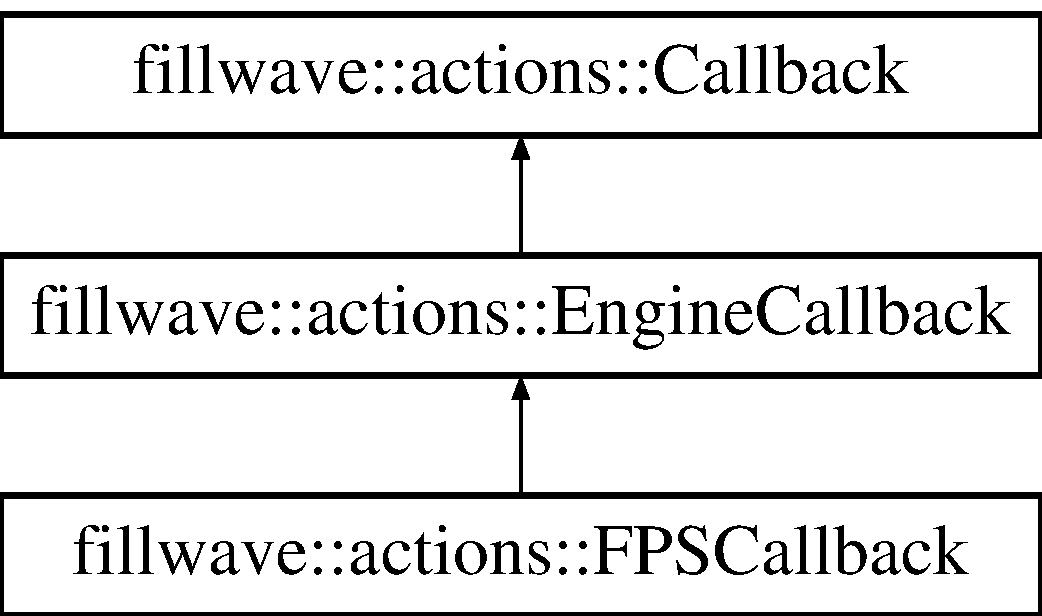
\includegraphics[height=3.000000cm]{classfillwave_1_1actions_1_1FPSCallback}
\end{center}
\end{figure}
\subsection*{Public Member Functions}
\begin{DoxyCompactItemize}
\item 
\hypertarget{classfillwave_1_1actions_1_1FPSCallback_a87075ddb053a3dc0485fc6571e7782bc}{}{\bfseries F\+P\+S\+Callback} (p\+Text text)\label{classfillwave_1_1actions_1_1FPSCallback_a87075ddb053a3dc0485fc6571e7782bc}

\item 
\hypertarget{classfillwave_1_1actions_1_1FPSCallback_a85cd3c5affa2850c49f017a1a070faeb}{}void {\bfseries perform} (\hyperlink{classfillwave_1_1Engine}{Engine} $\ast$engine, \hyperlink{classfillwave_1_1actions_1_1EventType}{Event\+Type} $\ast$event)\label{classfillwave_1_1actions_1_1FPSCallback_a85cd3c5affa2850c49f017a1a070faeb}

\end{DoxyCompactItemize}


\subsection{Detailed Description}
\hyperlink{classfillwave_1_1actions_1_1ItemCallback}{Item\+Callback} to display and refresh F\+P\+S as a renderable text. 

The documentation for this class was generated from the following file\+:\begin{DoxyCompactItemize}
\item 
/home/filip/\+Projects/fillwave/inc/fillwave/actions/F\+P\+S\+Callback.\+h\end{DoxyCompactItemize}

\hypertarget{classfillwave_1_1core_1_1Framebuffer}{}\section{fillwave\+:\+:core\+:\+:Framebuffer Class Reference}
\label{classfillwave_1_1core_1_1Framebuffer}\index{fillwave\+::core\+::\+Framebuffer@{fillwave\+::core\+::\+Framebuffer}}


Framebuffer\+Object -\/ F\+O.  




{\ttfamily \#include $<$Framebuffer.\+h$>$}

Inheritance diagram for fillwave\+:\+:core\+:\+:Framebuffer\+:\begin{figure}[H]
\begin{center}
\leavevmode
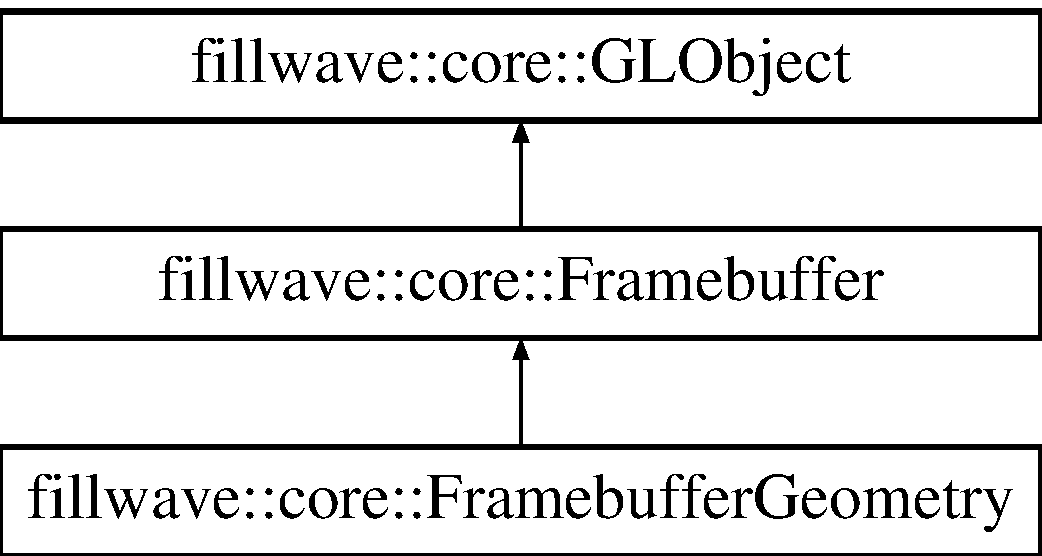
\includegraphics[height=3.000000cm]{classfillwave_1_1core_1_1Framebuffer}
\end{center}
\end{figure}
\subsection*{Public Member Functions}
\begin{DoxyCompactItemize}
\item 
\hypertarget{classfillwave_1_1core_1_1Framebuffer_a3f1dae680d984445933e058f87d555a5}{}{\bfseries Framebuffer} (G\+Lsizei how\+Many=1)\label{classfillwave_1_1core_1_1Framebuffer_a3f1dae680d984445933e058f87d555a5}

\item 
\hypertarget{classfillwave_1_1core_1_1Framebuffer_a286eb0ba19be0c10bde38abbc84e879c}{}void {\bfseries bind} (G\+Luint id=0) const \label{classfillwave_1_1core_1_1Framebuffer_a286eb0ba19be0c10bde38abbc84e879c}

\item 
\hypertarget{classfillwave_1_1core_1_1Framebuffer_a79034e3c1b7aee0df170fa066e89ffca}{}void {\bfseries attach\+Texture2\+D} (G\+Lenum attachment, G\+Lenum target, G\+Luint texture\+Handle)\label{classfillwave_1_1core_1_1Framebuffer_a79034e3c1b7aee0df170fa066e89ffca}

\item 
\hypertarget{classfillwave_1_1core_1_1Framebuffer_a79289cfb07a09dfaa05081591fee7660}{}void {\bfseries attach\+Texture2\+D\+Draw} (G\+Lenum attachment, G\+Lenum target, G\+Luint texture\+Handle)\label{classfillwave_1_1core_1_1Framebuffer_a79289cfb07a09dfaa05081591fee7660}

\item 
\hypertarget{classfillwave_1_1core_1_1Framebuffer_a5003cfbba50a81d0f790898b52623157}{}void {\bfseries bind\+For\+Writing} (G\+Luint id=0) const \label{classfillwave_1_1core_1_1Framebuffer_a5003cfbba50a81d0f790898b52623157}

\item 
\hypertarget{classfillwave_1_1core_1_1Framebuffer_a4493a9b9784a616c76cbe25119f69217}{}void {\bfseries bind\+For\+Reading} (G\+Luint id=0) const \label{classfillwave_1_1core_1_1Framebuffer_a4493a9b9784a616c76cbe25119f69217}

\item 
\hypertarget{classfillwave_1_1core_1_1Framebuffer_a26da0dddb7ae7fcfd2fe180243c29e87}{}void {\bfseries set\+Read\+Color\+Attachment} (G\+Luint attachment\+Color)\label{classfillwave_1_1core_1_1Framebuffer_a26da0dddb7ae7fcfd2fe180243c29e87}

\item 
\hypertarget{classfillwave_1_1core_1_1Framebuffer_ac7bcb86cec3e06263447b3fdf38c8300}{}void {\bfseries set\+Read\+Depth\+Attachment} ()\label{classfillwave_1_1core_1_1Framebuffer_ac7bcb86cec3e06263447b3fdf38c8300}

\item 
\hypertarget{classfillwave_1_1core_1_1Framebuffer_a3cb3180efee34beb841f2b1a4065d3e7}{}virtual void {\bfseries reload} ()\label{classfillwave_1_1core_1_1Framebuffer_a3cb3180efee34beb841f2b1a4065d3e7}

\end{DoxyCompactItemize}
\subsection*{Static Public Member Functions}
\begin{DoxyCompactItemize}
\item 
\hypertarget{classfillwave_1_1core_1_1Framebuffer_afebebaa9b9a6a5d9ab4ade9f669258b9}{}static void {\bfseries bind\+Screen\+Framebuffer} ()\label{classfillwave_1_1core_1_1Framebuffer_afebebaa9b9a6a5d9ab4ade9f669258b9}

\item 
\hypertarget{classfillwave_1_1core_1_1Framebuffer_a4402d0803909593d64e52ca3cb228bbf}{}static void {\bfseries bind\+Screen\+Framebuffer\+For\+Reading} ()\label{classfillwave_1_1core_1_1Framebuffer_a4402d0803909593d64e52ca3cb228bbf}

\item 
\hypertarget{classfillwave_1_1core_1_1Framebuffer_aa614fc524a61de7839fd7cca66c38543}{}static void {\bfseries bind\+Screen\+Framebuffer\+For\+Writing} ()\label{classfillwave_1_1core_1_1Framebuffer_aa614fc524a61de7839fd7cca66c38543}

\end{DoxyCompactItemize}
\subsection*{Additional Inherited Members}


\subsection{Detailed Description}
Framebuffer\+Object -\/ F\+O. 

The documentation for this class was generated from the following file\+:\begin{DoxyCompactItemize}
\item 
/home/filip/\+Projects/fillwave/inc/fillwave/core/rendering/Framebuffer.\+h\end{DoxyCompactItemize}

\hypertarget{classfillwave_1_1core_1_1FramebufferGeometry}{}\section{fillwave\+:\+:core\+:\+:Framebuffer\+Geometry Class Reference}
\label{classfillwave_1_1core_1_1FramebufferGeometry}\index{fillwave\+::core\+::\+Framebuffer\+Geometry@{fillwave\+::core\+::\+Framebuffer\+Geometry}}


\hyperlink{classfillwave_1_1core_1_1Framebuffer}{Framebuffer} with multiple color and depth attachments.  




{\ttfamily \#include $<$Framebuffer\+Geometry.\+h$>$}

Inheritance diagram for fillwave\+:\+:core\+:\+:Framebuffer\+Geometry\+:\begin{figure}[H]
\begin{center}
\leavevmode
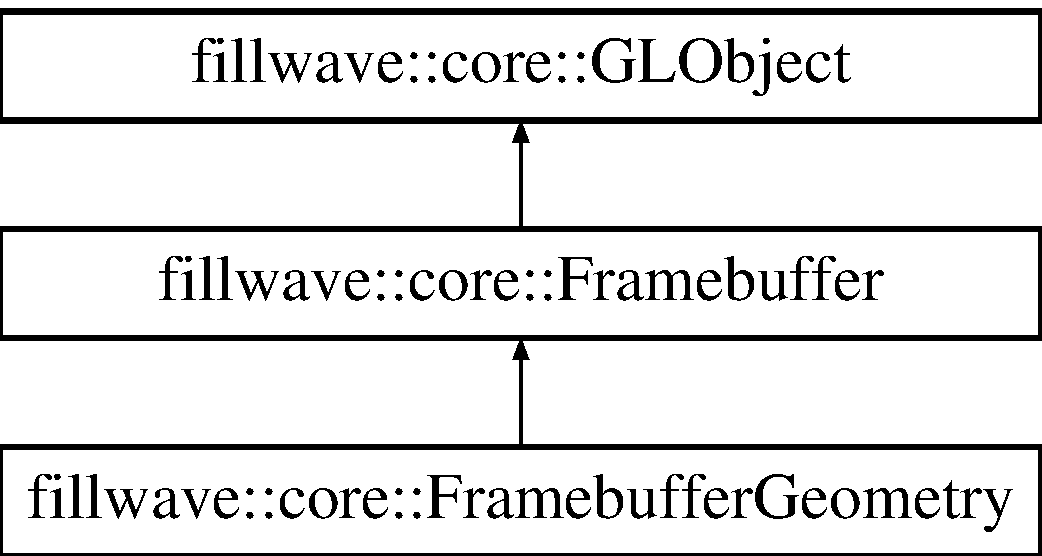
\includegraphics[height=3.000000cm]{classfillwave_1_1core_1_1FramebufferGeometry}
\end{center}
\end{figure}
\subsection*{Public Member Functions}
\begin{DoxyCompactItemize}
\item 
\hypertarget{classfillwave_1_1core_1_1FramebufferGeometry_a59763606fd9b16695580349c22edc9ae}{}{\bfseries Framebuffer\+Geometry} (\hyperlink{classfillwave_1_1manager_1_1TextureManager}{manager\+::\+Texture\+Manager} $\ast$manager, G\+Luint width, G\+Luint height, G\+Luint color\+Buffers, G\+Luint depth\+Buffers)\label{classfillwave_1_1core_1_1FramebufferGeometry_a59763606fd9b16695580349c22edc9ae}

\item 
\hypertarget{classfillwave_1_1core_1_1FramebufferGeometry_a749f0d5db2e911266fa5ec233b67f23f}{}void {\bfseries bind\+Attachments} ()\label{classfillwave_1_1core_1_1FramebufferGeometry_a749f0d5db2e911266fa5ec233b67f23f}

\item 
\hypertarget{classfillwave_1_1core_1_1FramebufferGeometry_a3d5766e2a836120d1f4c733b6421794a}{}void {\bfseries set\+Attachments} ()\label{classfillwave_1_1core_1_1FramebufferGeometry_a3d5766e2a836120d1f4c733b6421794a}

\item 
\hypertarget{classfillwave_1_1core_1_1FramebufferGeometry_af285b90c3782003d5d98b8e618216c3b}{}void {\bfseries set\+Attachment\+Stencil\+Depth} ()\label{classfillwave_1_1core_1_1FramebufferGeometry_af285b90c3782003d5d98b8e618216c3b}

\item 
\hypertarget{classfillwave_1_1core_1_1FramebufferGeometry_a71047970c333245214cae3f054c42799}{}void {\bfseries set\+Attachment\+Summary\+For\+Reading} ()\label{classfillwave_1_1core_1_1FramebufferGeometry_a71047970c333245214cae3f054c42799}

\item 
\hypertarget{classfillwave_1_1core_1_1FramebufferGeometry_a099fde18e37ff62215bea3ba6b736aa2}{}void {\bfseries set\+Attachment\+Summary\+For\+Writing} ()\label{classfillwave_1_1core_1_1FramebufferGeometry_a099fde18e37ff62215bea3ba6b736aa2}

\item 
\hypertarget{classfillwave_1_1core_1_1FramebufferGeometry_a5db11b693de9a4b8861f490fe861ef63}{}void {\bfseries resize} (G\+Luint width, G\+Luint height)\label{classfillwave_1_1core_1_1FramebufferGeometry_a5db11b693de9a4b8861f490fe861ef63}

\item 
\hypertarget{classfillwave_1_1core_1_1FramebufferGeometry_af6f8fa2c63b223d1e6db143fc523f09e}{}void {\bfseries reload} ()\label{classfillwave_1_1core_1_1FramebufferGeometry_af6f8fa2c63b223d1e6db143fc523f09e}

\end{DoxyCompactItemize}
\subsection*{Additional Inherited Members}


\subsection{Detailed Description}
\hyperlink{classfillwave_1_1core_1_1Framebuffer}{Framebuffer} with multiple color and depth attachments. 

The documentation for this class was generated from the following file\+:\begin{DoxyCompactItemize}
\item 
/home/filip/\+Projects/fillwave/inc/fillwave/core/rendering/Framebuffer\+Geometry.\+h\end{DoxyCompactItemize}

\hypertarget{classfillwave_1_1core_1_1GLObject}{}\section{fillwave\+:\+:core\+:\+:G\+L\+Object Class Reference}
\label{classfillwave_1_1core_1_1GLObject}\index{fillwave\+::core\+::\+G\+L\+Object@{fillwave\+::core\+::\+G\+L\+Object}}


Base class for all Open\+G\+L objects not related to pipeline.  




{\ttfamily \#include $<$G\+L\+Object.\+h$>$}

Inheritance diagram for fillwave\+:\+:core\+:\+:G\+L\+Object\+:\begin{figure}[H]
\begin{center}
\leavevmode
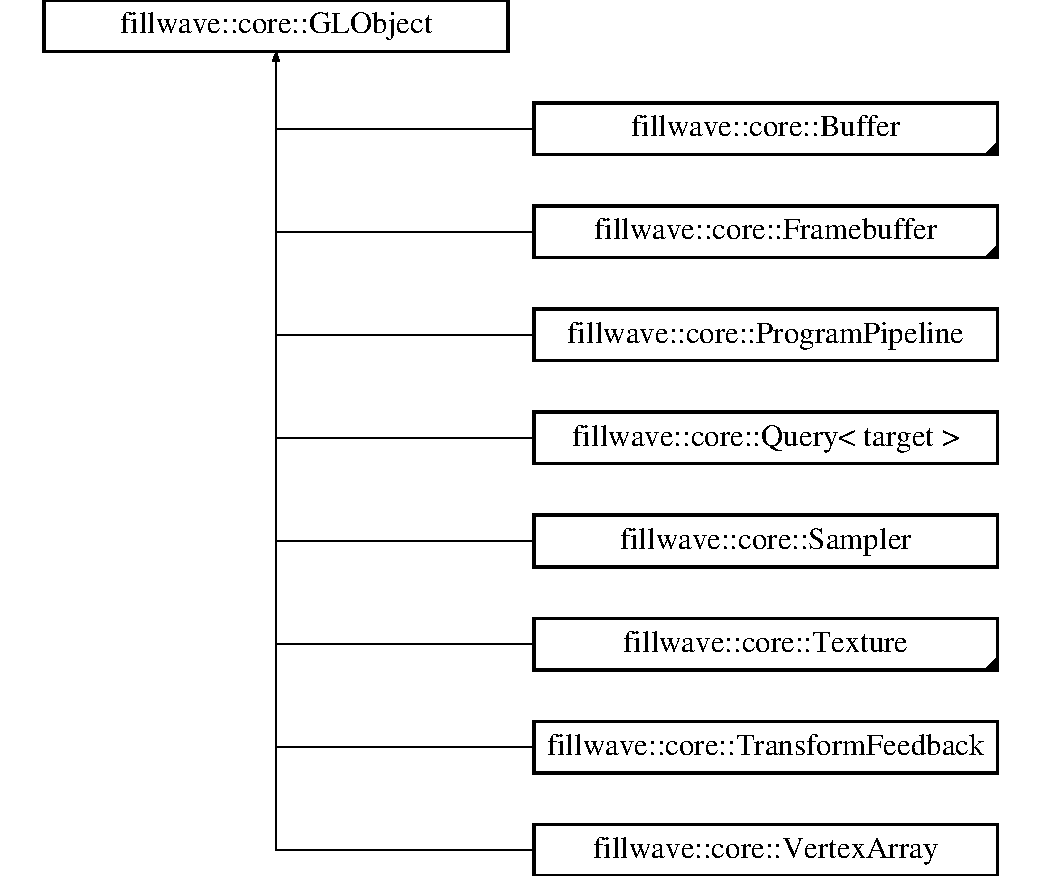
\includegraphics[height=9.000000cm]{classfillwave_1_1core_1_1GLObject}
\end{center}
\end{figure}
\subsection*{Public Member Functions}
\begin{DoxyCompactItemize}
\item 
\hypertarget{classfillwave_1_1core_1_1GLObject_adf54dafb1a5b9f1ef5e6f6a4a995abd1}{}{\bfseries G\+L\+Object} (G\+Lsizei how\+Many)\label{classfillwave_1_1core_1_1GLObject_adf54dafb1a5b9f1ef5e6f6a4a995abd1}

\item 
\hypertarget{classfillwave_1_1core_1_1GLObject_ae0e1c865347204ed8353cc7a802640dd}{}G\+Luint {\bfseries get\+Handle} (G\+Luint id=0)\label{classfillwave_1_1core_1_1GLObject_ae0e1c865347204ed8353cc7a802640dd}

\item 
\hypertarget{classfillwave_1_1core_1_1GLObject_a7985f8f984a1b6f6b018cdedcbab387c}{}virtual void {\bfseries reload} ()=0\label{classfillwave_1_1core_1_1GLObject_a7985f8f984a1b6f6b018cdedcbab387c}

\end{DoxyCompactItemize}
\subsection*{Protected Attributes}
\begin{DoxyCompactItemize}
\item 
\hypertarget{classfillwave_1_1core_1_1GLObject_a005f281fe10e1af954695452528c2a8d}{}G\+Lsizei {\bfseries m\+How\+Many}\label{classfillwave_1_1core_1_1GLObject_a005f281fe10e1af954695452528c2a8d}

\item 
\hypertarget{classfillwave_1_1core_1_1GLObject_a44efc7a7b19fc7012fe582fe4e9c3cc0}{}G\+Luint $\ast$ {\bfseries m\+Handles}\label{classfillwave_1_1core_1_1GLObject_a44efc7a7b19fc7012fe582fe4e9c3cc0}

\end{DoxyCompactItemize}


\subsection{Detailed Description}
Base class for all Open\+G\+L objects not related to pipeline. 

The documentation for this class was generated from the following file\+:\begin{DoxyCompactItemize}
\item 
/home/filip/\+Projects/fillwave/inc/fillwave/core/G\+L\+Object.\+h\end{DoxyCompactItemize}

\hypertarget{classfillwave_1_1particles_1_1Impostor}{}\section{fillwave\+:\+:particles\+:\+:Impostor Class Reference}
\label{classfillwave_1_1particles_1_1Impostor}\index{fillwave\+::particles\+::\+Impostor@{fillwave\+::particles\+::\+Impostor}}


Drawable Entity built by fragment shader. Time limited.  




{\ttfamily \#include $<$Impostor.\+h$>$}

Inheritance diagram for fillwave\+:\+:particles\+:\+:Impostor\+:\begin{figure}[H]
\begin{center}
\leavevmode
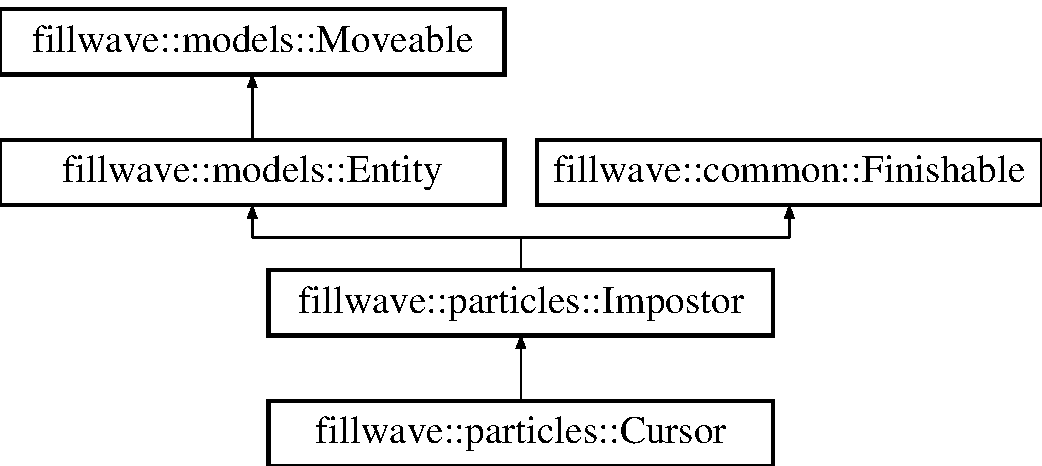
\includegraphics[height=4.000000cm]{classfillwave_1_1particles_1_1Impostor}
\end{center}
\end{figure}
\subsection*{Public Member Functions}
\begin{DoxyCompactItemize}
\item 
\hypertarget{classfillwave_1_1particles_1_1Impostor_a899285ac9e0ef5aae15dd7c02510ac2b}{}{\bfseries Impostor} (\hyperlink{classfillwave_1_1Engine}{Engine} $\ast$engine, G\+Lfloat lifetime, G\+Lfloat size, p\+Texture texture=p\+Texture(), G\+Lenum blending\+Source=G\+L\+\_\+\+S\+R\+C\+\_\+\+A\+L\+P\+H\+A, G\+Lenum blending\+Destination=G\+L\+\_\+\+O\+N\+E\+\_\+\+M\+I\+N\+U\+S\+\_\+\+S\+R\+C\+\_\+\+A\+L\+P\+H\+A)\label{classfillwave_1_1particles_1_1Impostor_a899285ac9e0ef5aae15dd7c02510ac2b}

\item 
\hypertarget{classfillwave_1_1particles_1_1Impostor_ae45f2c8edccb5546f4eef14c7aaf5c99}{}virtual void {\bfseries draw} (\hyperlink{classfillwave_1_1space_1_1Camera}{space\+::\+Camera} \&camera)\label{classfillwave_1_1particles_1_1Impostor_ae45f2c8edccb5546f4eef14c7aaf5c99}

\end{DoxyCompactItemize}
\subsection*{Protected Member Functions}
\begin{DoxyCompactItemize}
\item 
\hypertarget{classfillwave_1_1particles_1_1Impostor_a2f15380e3bb0bfe858beb3f907c1d9b7}{}void {\bfseries core\+Draw} ()\label{classfillwave_1_1particles_1_1Impostor_a2f15380e3bb0bfe858beb3f907c1d9b7}

\end{DoxyCompactItemize}
\subsection*{Protected Attributes}
\begin{DoxyCompactItemize}
\item 
\hypertarget{classfillwave_1_1particles_1_1Impostor_a53809584e50549b81179d1a364271fe1}{}p\+Program {\bfseries m\+Program}\label{classfillwave_1_1particles_1_1Impostor_a53809584e50549b81179d1a364271fe1}

\item 
\hypertarget{classfillwave_1_1particles_1_1Impostor_a4c0d1d324afd9ed7a50f93237d3c2481}{}G\+Lfloat {\bfseries m\+Size}\label{classfillwave_1_1particles_1_1Impostor_a4c0d1d324afd9ed7a50f93237d3c2481}

\end{DoxyCompactItemize}


\subsection{Detailed Description}
Drawable Entity built by fragment shader. Time limited. 

The documentation for this class was generated from the following file\+:\begin{DoxyCompactItemize}
\item 
/home/filip/\+Projects/fillwave/inc/fillwave/particles/Impostor.\+h\end{DoxyCompactItemize}

\hypertarget{classfillwave_1_1core_1_1IndexBuffer}{}\section{fillwave\+:\+:core\+:\+:Index\+Buffer Class Reference}
\label{classfillwave_1_1core_1_1IndexBuffer}\index{fillwave\+::core\+::\+Index\+Buffer@{fillwave\+::core\+::\+Index\+Buffer}}


Index\+Buffer\+Object -\/ I\+B\+O.  




{\ttfamily \#include $<$Index\+Buffer.\+h$>$}

Inheritance diagram for fillwave\+:\+:core\+:\+:Index\+Buffer\+:\begin{figure}[H]
\begin{center}
\leavevmode
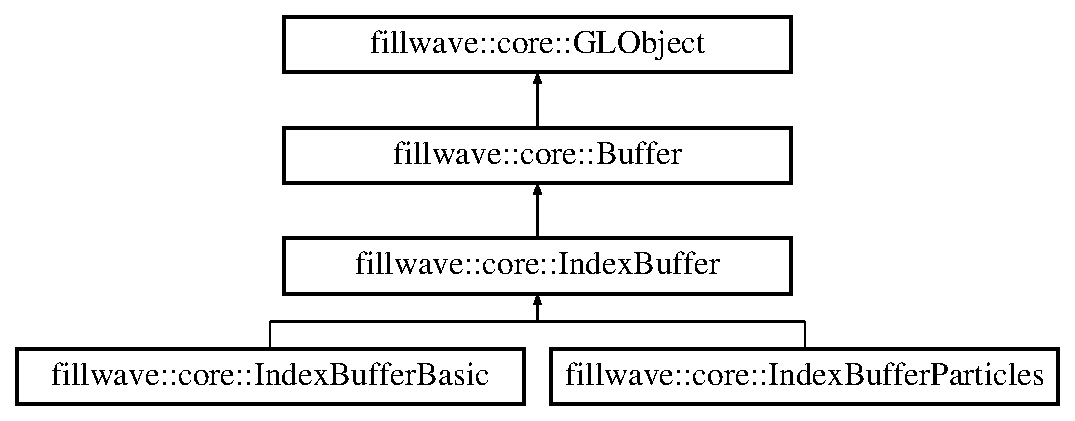
\includegraphics[height=4.000000cm]{classfillwave_1_1core_1_1IndexBuffer}
\end{center}
\end{figure}
\subsection*{Public Member Functions}
\begin{DoxyCompactItemize}
\item 
\hypertarget{classfillwave_1_1core_1_1IndexBuffer_a93b5036c653fcb090013d6395bcae6c5}{}{\bfseries Index\+Buffer} (G\+Luint elements, G\+Luint data\+Store\+Modification)\label{classfillwave_1_1core_1_1IndexBuffer_a93b5036c653fcb090013d6395bcae6c5}

\end{DoxyCompactItemize}
\subsection*{Protected Attributes}
\begin{DoxyCompactItemize}
\item 
\hypertarget{classfillwave_1_1core_1_1IndexBuffer_adbb519ab404fbfd8399bdd0250dc17a1}{}std\+::vector$<$ G\+Luint $>$ {\bfseries m\+Data\+Indices}\label{classfillwave_1_1core_1_1IndexBuffer_adbb519ab404fbfd8399bdd0250dc17a1}

\end{DoxyCompactItemize}
\subsection*{Additional Inherited Members}


\subsection{Detailed Description}
Index\+Buffer\+Object -\/ I\+B\+O. 

The documentation for this class was generated from the following file\+:\begin{DoxyCompactItemize}
\item 
/home/filip/\+Projects/fillwave/inc/fillwave/core/buffers/Index\+Buffer.\+h\end{DoxyCompactItemize}

\hypertarget{classfillwave_1_1core_1_1IndexBufferBasic}{}\section{fillwave\+:\+:core\+:\+:Index\+Buffer\+Basic Class Reference}
\label{classfillwave_1_1core_1_1IndexBufferBasic}\index{fillwave\+::core\+::\+Index\+Buffer\+Basic@{fillwave\+::core\+::\+Index\+Buffer\+Basic}}


\hyperlink{classfillwave_1_1core_1_1IndexBuffer}{Index\+Buffer} for regular usage.  




{\ttfamily \#include $<$Index\+Buffer\+Basic.\+h$>$}

Inheritance diagram for fillwave\+:\+:core\+:\+:Index\+Buffer\+Basic\+:\begin{figure}[H]
\begin{center}
\leavevmode
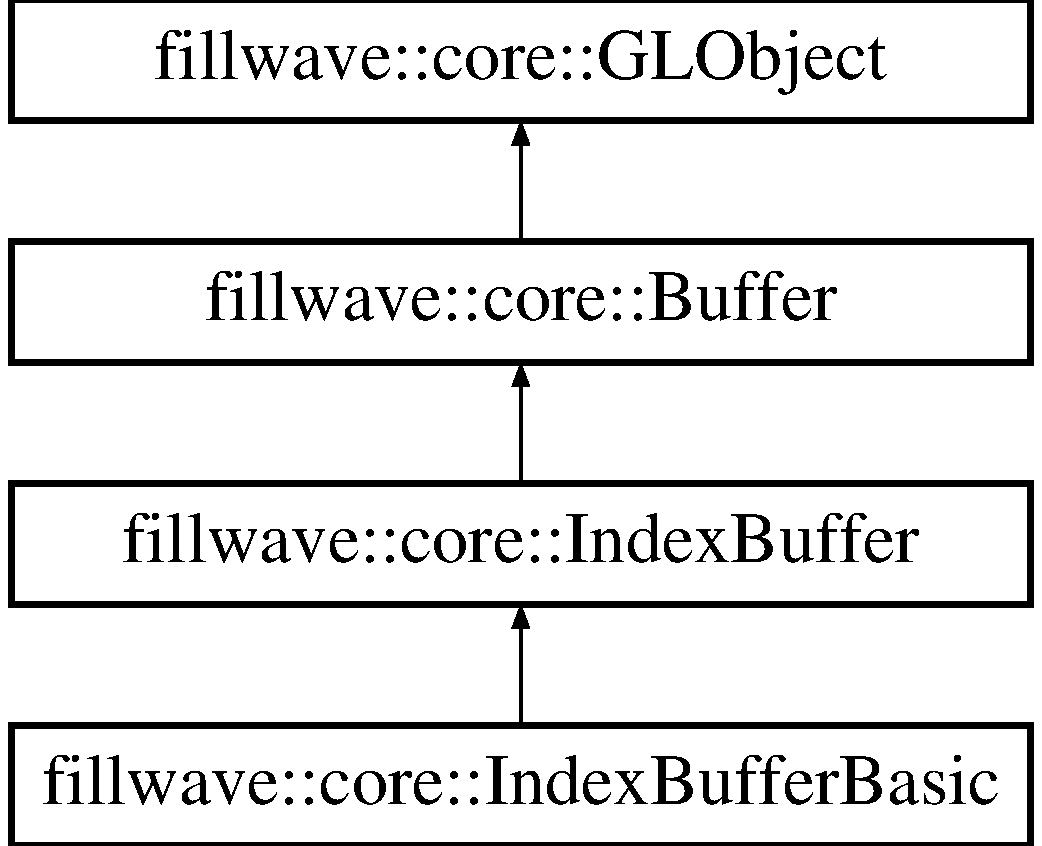
\includegraphics[height=4.000000cm]{classfillwave_1_1core_1_1IndexBufferBasic}
\end{center}
\end{figure}
\subsection*{Public Member Functions}
\begin{DoxyCompactItemize}
\item 
\hypertarget{classfillwave_1_1core_1_1IndexBufferBasic_ae008135e437a26363f46be5eac681e14}{}{\bfseries Index\+Buffer\+Basic} (std\+::vector$<$ G\+Luint $>$ \&data, G\+Luint data\+Store\+Modification=G\+L\+\_\+\+S\+T\+A\+T\+I\+C\+\_\+\+D\+R\+A\+W)\label{classfillwave_1_1core_1_1IndexBufferBasic_ae008135e437a26363f46be5eac681e14}

\item 
\hypertarget{classfillwave_1_1core_1_1IndexBufferBasic_adc40119fe347fc71cc04e1e70adb1f03}{}{\bfseries Index\+Buffer\+Basic} (const f\+Mesh $\ast$shape, G\+Luint data\+Store\+Modification=G\+L\+\_\+\+S\+T\+A\+T\+I\+C\+\_\+\+D\+R\+A\+W)\label{classfillwave_1_1core_1_1IndexBufferBasic_adc40119fe347fc71cc04e1e70adb1f03}

\item 
\hypertarget{classfillwave_1_1core_1_1IndexBufferBasic_addcddfa772344e0d71abcd269a416425}{}{\footnotesize template$<$class T $>$ }\\{\bfseries Index\+Buffer\+Basic} (\hyperlink{classfillwave_1_1models_1_1Shape}{models\+::\+Shape}$<$ T $>$ \&shape, G\+Luint data\+Store\+Modification=G\+L\+\_\+\+S\+T\+A\+T\+I\+C\+\_\+\+D\+R\+A\+W)\label{classfillwave_1_1core_1_1IndexBufferBasic_addcddfa772344e0d71abcd269a416425}

\item 
\hypertarget{classfillwave_1_1core_1_1IndexBufferBasic_a94e49eedf7f174df1c8cd6da229edf91}{}void {\bfseries load\+Element} (G\+Luint element)\label{classfillwave_1_1core_1_1IndexBufferBasic_a94e49eedf7f174df1c8cd6da229edf91}

\end{DoxyCompactItemize}
\subsection*{Additional Inherited Members}


\subsection{Detailed Description}
\hyperlink{classfillwave_1_1core_1_1IndexBuffer}{Index\+Buffer} for regular usage. 

The documentation for this class was generated from the following file\+:\begin{DoxyCompactItemize}
\item 
/home/filip/\+Projects/fillwave/inc/fillwave/core/buffers/Index\+Buffer\+Basic.\+h\end{DoxyCompactItemize}

\hypertarget{classfillwave_1_1core_1_1IndexBufferParticles}{}\section{fillwave\+:\+:core\+:\+:Index\+Buffer\+Particles Class Reference}
\label{classfillwave_1_1core_1_1IndexBufferParticles}\index{fillwave\+::core\+::\+Index\+Buffer\+Particles@{fillwave\+::core\+::\+Index\+Buffer\+Particles}}


I\+B\+O to use with particles.  




{\ttfamily \#include $<$Index\+Buffer\+Particles.\+h$>$}

Inheritance diagram for fillwave\+:\+:core\+:\+:Index\+Buffer\+Particles\+:\begin{figure}[H]
\begin{center}
\leavevmode
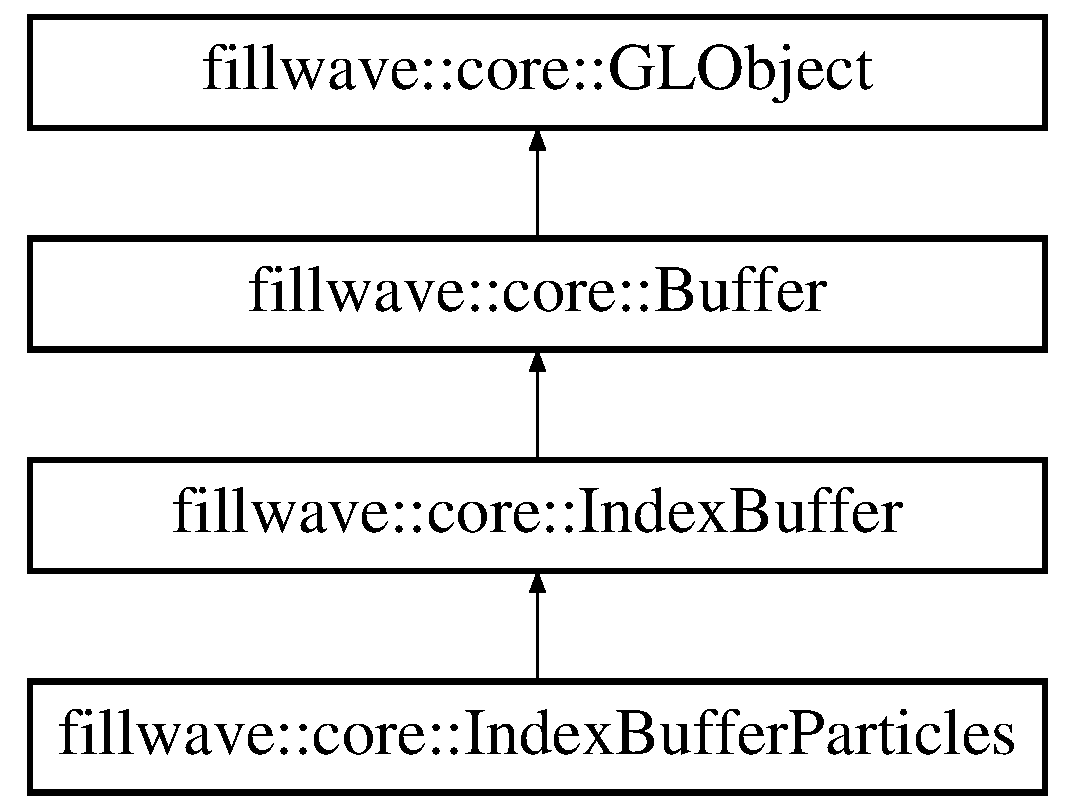
\includegraphics[height=4.000000cm]{classfillwave_1_1core_1_1IndexBufferParticles}
\end{center}
\end{figure}
\subsection*{Public Member Functions}
\begin{DoxyCompactItemize}
\item 
\hypertarget{classfillwave_1_1core_1_1IndexBufferParticles_a8b4f3f8f009acc1f253eee32d85e74c4}{}{\bfseries Index\+Buffer\+Particles} (G\+Luint elements)\label{classfillwave_1_1core_1_1IndexBufferParticles_a8b4f3f8f009acc1f253eee32d85e74c4}

\item 
\hypertarget{classfillwave_1_1core_1_1IndexBufferParticles_aef693f4fd505ec973a6270a6038de07a}{}G\+Luint $\ast$ {\bfseries get\+Data\+Internal} ()\label{classfillwave_1_1core_1_1IndexBufferParticles_aef693f4fd505ec973a6270a6038de07a}

\end{DoxyCompactItemize}
\subsection*{Additional Inherited Members}


\subsection{Detailed Description}
I\+B\+O to use with particles. 

The documentation for this class was generated from the following file\+:\begin{DoxyCompactItemize}
\item 
/home/filip/\+Projects/fillwave/inc/fillwave/core/buffers/Index\+Buffer\+Particles.\+h\end{DoxyCompactItemize}

\hypertarget{classfillwave_1_1actions_1_1ItemCallback}{}\section{fillwave\+:\+:actions\+:\+:Item\+Callback Class Reference}
\label{classfillwave_1_1actions_1_1ItemCallback}\index{fillwave\+::actions\+::\+Item\+Callback@{fillwave\+::actions\+::\+Item\+Callback}}


Base for item callbacks.  




{\ttfamily \#include $<$Item\+Callback.\+h$>$}

Inheritance diagram for fillwave\+:\+:actions\+:\+:Item\+Callback\+:\begin{figure}[H]
\begin{center}
\leavevmode
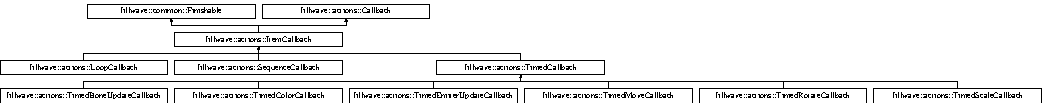
\includegraphics[height=1.377614cm]{classfillwave_1_1actions_1_1ItemCallback}
\end{center}
\end{figure}
\subsection*{Public Member Functions}
\begin{DoxyCompactItemize}
\item 
\hypertarget{classfillwave_1_1actions_1_1ItemCallback_a6973e37a4848cc91a723c637765edb49}{}{\bfseries Item\+Callback} (e\+Event\+Type event\+Type, float time\+To\+Finish=F\+I\+L\+L\+W\+A\+V\+E\+\_\+\+E\+N\+D\+L\+E\+S\+S)\label{classfillwave_1_1actions_1_1ItemCallback_a6973e37a4848cc91a723c637765edb49}

\item 
\hypertarget{classfillwave_1_1actions_1_1ItemCallback_aecdcaa43453d5dd262f1c15fe3eb993a}{}virtual void {\bfseries perform} (\hyperlink{classfillwave_1_1actions_1_1EventType}{Event\+Type} $\ast$event)=0\label{classfillwave_1_1actions_1_1ItemCallback_aecdcaa43453d5dd262f1c15fe3eb993a}

\item 
\hypertarget{classfillwave_1_1actions_1_1ItemCallback_acc05ed722cfc8382a366d3bfc6d4c826}{}bool {\bfseries is\+Enabled} ()\label{classfillwave_1_1actions_1_1ItemCallback_acc05ed722cfc8382a366d3bfc6d4c826}

\item 
\hypertarget{classfillwave_1_1actions_1_1ItemCallback_a4c9b7e5cfd4140bd839d4cf32acad4d8}{}void {\bfseries enable} ()\label{classfillwave_1_1actions_1_1ItemCallback_a4c9b7e5cfd4140bd839d4cf32acad4d8}

\item 
\hypertarget{classfillwave_1_1actions_1_1ItemCallback_abd8d654db1ccca4d04bd74c6244608c7}{}void {\bfseries disable} ()\label{classfillwave_1_1actions_1_1ItemCallback_abd8d654db1ccca4d04bd74c6244608c7}

\end{DoxyCompactItemize}
\subsection*{Protected Attributes}
\begin{DoxyCompactItemize}
\item 
\hypertarget{classfillwave_1_1actions_1_1ItemCallback_a5eeb5a6801cf0bfc654610752d85652c}{}bool {\bfseries m\+Enabled}\label{classfillwave_1_1actions_1_1ItemCallback_a5eeb5a6801cf0bfc654610752d85652c}

\end{DoxyCompactItemize}


\subsection{Detailed Description}
Base for item callbacks. 

The documentation for this class was generated from the following file\+:\begin{DoxyCompactItemize}
\item 
/home/filip/\+Projects/fillwave/inc/fillwave/actions/Item\+Callback.\+h\end{DoxyCompactItemize}

\hypertarget{classfillwave_1_1animation_1_1Key}{}\section{fillwave\+:\+:animation\+:\+:Key$<$ T $>$ Class Template Reference}
\label{classfillwave_1_1animation_1_1Key}\index{fillwave\+::animation\+::\+Key$<$ T $>$@{fillwave\+::animation\+::\+Key$<$ T $>$}}


Base for all animation keys.  




{\ttfamily \#include $<$Key.\+h$>$}

\subsection*{Public Member Functions}
\begin{DoxyCompactItemize}
\item 
\hypertarget{classfillwave_1_1animation_1_1Key_aee5c9d28fdf14878b69f95dc203faada}{}{\bfseries Key} (float time\+Stamp, T value)\label{classfillwave_1_1animation_1_1Key_aee5c9d28fdf14878b69f95dc203faada}

\end{DoxyCompactItemize}
\subsection*{Public Attributes}
\begin{DoxyCompactItemize}
\item 
\hypertarget{classfillwave_1_1animation_1_1Key_ae64b38b95a06e3874520bd006452be2a}{}float {\bfseries m\+Time}\label{classfillwave_1_1animation_1_1Key_ae64b38b95a06e3874520bd006452be2a}

\item 
\hypertarget{classfillwave_1_1animation_1_1Key_a3a656264ec7dd546029e87c6a819c277}{}T {\bfseries m\+Value}\label{classfillwave_1_1animation_1_1Key_a3a656264ec7dd546029e87c6a819c277}

\end{DoxyCompactItemize}


\subsection{Detailed Description}
\subsubsection*{template$<$class T$>$class fillwave\+::animation\+::\+Key$<$ T $>$}

Base for all animation keys. 

The documentation for this class was generated from the following file\+:\begin{DoxyCompactItemize}
\item 
/home/filip/\+Projects/fillwave/inc/fillwave/animation/Key.\+h\end{DoxyCompactItemize}

\hypertarget{classfillwave_1_1actions_1_1KeyboardEvent}{}\section{fillwave\+:\+:actions\+:\+:Keyboard\+Event Struct Reference}
\label{classfillwave_1_1actions_1_1KeyboardEvent}\index{fillwave\+::actions\+::\+Keyboard\+Event@{fillwave\+::actions\+::\+Keyboard\+Event}}


\hyperlink{classfillwave_1_1actions_1_1Event}{Event} introduced when something happens with the key.  




{\ttfamily \#include $<$Keyboard\+Event.\+h$>$}

Inheritance diagram for fillwave\+:\+:actions\+:\+:Keyboard\+Event\+:\begin{figure}[H]
\begin{center}
\leavevmode
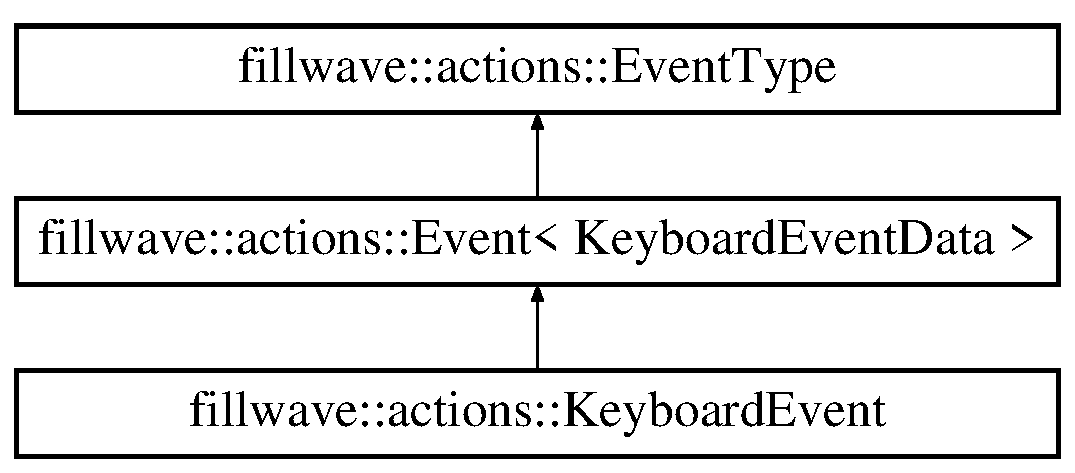
\includegraphics[height=3.000000cm]{classfillwave_1_1actions_1_1KeyboardEvent}
\end{center}
\end{figure}
\subsection*{Public Member Functions}
\begin{DoxyCompactItemize}
\item 
\hypertarget{classfillwave_1_1actions_1_1KeyboardEvent_afed8f8066a7a067a4fd846d070b505a2}{}{\bfseries Keyboard\+Event} (\hyperlink{structfillwave_1_1actions_1_1KeyboardEventData}{Keyboard\+Event\+Data} data)\label{classfillwave_1_1actions_1_1KeyboardEvent_afed8f8066a7a067a4fd846d070b505a2}

\end{DoxyCompactItemize}
\subsection*{Additional Inherited Members}


\subsection{Detailed Description}
\hyperlink{classfillwave_1_1actions_1_1Event}{Event} introduced when something happens with the key. 

The documentation for this struct was generated from the following file\+:\begin{DoxyCompactItemize}
\item 
/home/filip/\+Projects/fillwave/inc/fillwave/actions/Keyboard\+Event.\+h\end{DoxyCompactItemize}

\hypertarget{structfillwave_1_1actions_1_1KeyboardEventData}{}\section{fillwave\+:\+:actions\+:\+:Keyboard\+Event\+Data Struct Reference}
\label{structfillwave_1_1actions_1_1KeyboardEventData}\index{fillwave\+::actions\+::\+Keyboard\+Event\+Data@{fillwave\+::actions\+::\+Keyboard\+Event\+Data}}


\hyperlink{classfillwave_1_1actions_1_1Event}{Event} data structure to store the parameters of a key event.  




{\ttfamily \#include $<$Keyboard\+Event.\+h$>$}

\subsection*{Public Attributes}
\begin{DoxyCompactItemize}
\item 
\hypertarget{structfillwave_1_1actions_1_1KeyboardEventData_a8d9037dadc8c0d7c8b87f70c11959edc}{}int {\bfseries key}\label{structfillwave_1_1actions_1_1KeyboardEventData_a8d9037dadc8c0d7c8b87f70c11959edc}

\item 
\hypertarget{structfillwave_1_1actions_1_1KeyboardEventData_a2d86b8e3f90bafecce1d88e77f7bdfa9}{}int {\bfseries scan\+Code}\label{structfillwave_1_1actions_1_1KeyboardEventData_a2d86b8e3f90bafecce1d88e77f7bdfa9}

\item 
\hypertarget{structfillwave_1_1actions_1_1KeyboardEventData_acb22843a4b01911213a7acadc83a0181}{}int {\bfseries action}\label{structfillwave_1_1actions_1_1KeyboardEventData_acb22843a4b01911213a7acadc83a0181}

\item 
\hypertarget{structfillwave_1_1actions_1_1KeyboardEventData_a2e21c4f49415448ee5a5728026a2ddad}{}int {\bfseries mode}\label{structfillwave_1_1actions_1_1KeyboardEventData_a2e21c4f49415448ee5a5728026a2ddad}

\item 
\hypertarget{structfillwave_1_1actions_1_1KeyboardEventData_a71a6733e96b01688a12e4f5912587747}{}const e\+Event\+Type {\bfseries type} = e\+Event\+Type\+::key\label{structfillwave_1_1actions_1_1KeyboardEventData_a71a6733e96b01688a12e4f5912587747}

\end{DoxyCompactItemize}


\subsection{Detailed Description}
\hyperlink{classfillwave_1_1actions_1_1Event}{Event} data structure to store the parameters of a key event. 

The documentation for this struct was generated from the following file\+:\begin{DoxyCompactItemize}
\item 
/home/filip/\+Projects/fillwave/inc/fillwave/actions/Keyboard\+Event.\+h\end{DoxyCompactItemize}

\hypertarget{classfillwave_1_1space_1_1Light}{}\section{fillwave\+:\+:space\+:\+:Light Class Reference}
\label{classfillwave_1_1space_1_1Light}\index{fillwave\+::space\+::\+Light@{fillwave\+::space\+::\+Light}}


Base for all lights.  




{\ttfamily \#include $<$Light.\+h$>$}

Inheritance diagram for fillwave\+:\+:space\+:\+:Light\+:\begin{figure}[H]
\begin{center}
\leavevmode
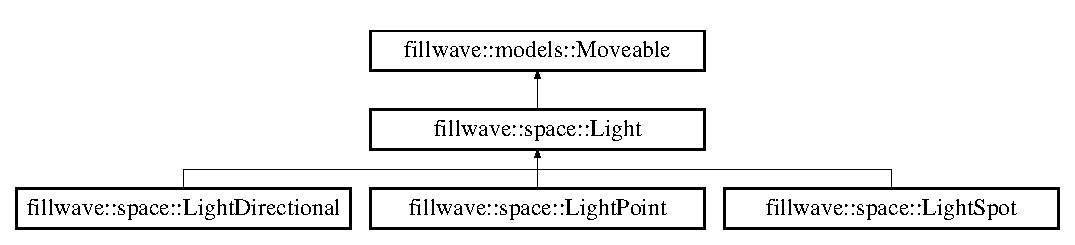
\includegraphics[height=2.842640cm]{classfillwave_1_1space_1_1Light}
\end{center}
\end{figure}
\subsection*{Public Member Functions}
\begin{DoxyCompactItemize}
\item 
\hypertarget{classfillwave_1_1space_1_1Light_a9c573c7a265fe319b180f5391cb00f3d}{}{\bfseries Light} (glm\+::vec3 position, glm\+::vec4 intensity, p\+Entity entity=p\+Entity())\label{classfillwave_1_1space_1_1Light_a9c573c7a265fe319b180f5391cb00f3d}

\item 
\hypertarget{classfillwave_1_1space_1_1Light_a71ca1937ed077045d9391ecabd592bcc}{}void {\bfseries update\+Entity} ()\label{classfillwave_1_1space_1_1Light_a71ca1937ed077045d9391ecabd592bcc}

\item 
\hypertarget{classfillwave_1_1space_1_1Light_a691880b4aae4e500eec7ca737dc1cce1}{}void {\bfseries set\+Attenuation} (\hyperlink{structfillwave_1_1space_1_1LightAttenuationData}{Light\+Attenuation\+Data} \&attenuation)\label{classfillwave_1_1space_1_1Light_a691880b4aae4e500eec7ca737dc1cce1}

\item 
\hypertarget{classfillwave_1_1space_1_1Light_abdaf623ab7a8ef8bddcba0a9e2440056}{}\hyperlink{structfillwave_1_1space_1_1LightAttenuationData}{Light\+Attenuation\+Data} {\bfseries get\+Attenuation} ()\label{classfillwave_1_1space_1_1Light_abdaf623ab7a8ef8bddcba0a9e2440056}

\item 
\hypertarget{classfillwave_1_1space_1_1Light_a7a7f79ec59bd6244811e0947bee4f3bc}{}void {\bfseries set\+Intensity} (glm\+::vec4 intensity)\label{classfillwave_1_1space_1_1Light_a7a7f79ec59bd6244811e0947bee4f3bc}

\item 
\hypertarget{classfillwave_1_1space_1_1Light_a2ca35e03003c95beaf607b84ed5e3c12}{}glm\+::vec4 {\bfseries get\+Intensity} ()\label{classfillwave_1_1space_1_1Light_a2ca35e03003c95beaf607b84ed5e3c12}

\item 
\hypertarget{classfillwave_1_1space_1_1Light_a5481eadd75b7a7725fba3fa062b73cf1}{}void {\bfseries set\+Entity} (p\+Entity entity)\label{classfillwave_1_1space_1_1Light_a5481eadd75b7a7725fba3fa062b73cf1}

\item 
\hypertarget{classfillwave_1_1space_1_1Light_aed87256495746c7b4a8e6c57474beaad}{}p\+Entity {\bfseries get\+Entity} ()\label{classfillwave_1_1space_1_1Light_aed87256495746c7b4a8e6c57474beaad}

\item 
\hypertarget{classfillwave_1_1space_1_1Light_a8a756bffdd299cd6bc2bfcc7f98fb230}{}void {\bfseries log} ()\label{classfillwave_1_1space_1_1Light_a8a756bffdd299cd6bc2bfcc7f98fb230}

\end{DoxyCompactItemize}
\subsection*{Protected Attributes}
\begin{DoxyCompactItemize}
\item 
\hypertarget{classfillwave_1_1space_1_1Light_a009157c29e3454b5893193fd3b796de1}{}p\+Entity {\bfseries m\+Entity}\label{classfillwave_1_1space_1_1Light_a009157c29e3454b5893193fd3b796de1}

\item 
\hypertarget{classfillwave_1_1space_1_1Light_ae52787955cd7c59c36e97b164a66843e}{}glm\+::vec4 {\bfseries m\+Intensity}\label{classfillwave_1_1space_1_1Light_ae52787955cd7c59c36e97b164a66843e}

\item 
\hypertarget{classfillwave_1_1space_1_1Light_ae095ec945b6b1ba28d36c3ef923c7189}{}\hyperlink{structfillwave_1_1space_1_1LightAttenuationData}{Light\+Attenuation\+Data} {\bfseries m\+Attenuation}\label{classfillwave_1_1space_1_1Light_ae095ec945b6b1ba28d36c3ef923c7189}

\end{DoxyCompactItemize}


\subsection{Detailed Description}
Base for all lights. 

The documentation for this class was generated from the following file\+:\begin{DoxyCompactItemize}
\item 
/home/filip/\+Projects/fillwave/inc/fillwave/space/Light.\+h\end{DoxyCompactItemize}

\hypertarget{structfillwave_1_1space_1_1LightAttenuationData}{}\section{fillwave\+:\+:space\+:\+:Light\+Attenuation\+Data Struct Reference}
\label{structfillwave_1_1space_1_1LightAttenuationData}\index{fillwave\+::space\+::\+Light\+Attenuation\+Data@{fillwave\+::space\+::\+Light\+Attenuation\+Data}}


\hyperlink{classfillwave_1_1space_1_1Light}{Light} attenuation data.  




{\ttfamily \#include $<$Light.\+h$>$}

\subsection*{Public Attributes}
\begin{DoxyCompactItemize}
\item 
\hypertarget{structfillwave_1_1space_1_1LightAttenuationData_ad353a42e530d6639ff16c02abae3db24}{}G\+Lfloat {\bfseries m\+Linear}\label{structfillwave_1_1space_1_1LightAttenuationData_ad353a42e530d6639ff16c02abae3db24}

\item 
\hypertarget{structfillwave_1_1space_1_1LightAttenuationData_ac49051c6fa1ae1641fb2fb9554a6d2be}{}G\+Lfloat {\bfseries m\+Exp}\label{structfillwave_1_1space_1_1LightAttenuationData_ac49051c6fa1ae1641fb2fb9554a6d2be}

\end{DoxyCompactItemize}


\subsection{Detailed Description}
\hyperlink{classfillwave_1_1space_1_1Light}{Light} attenuation data. 

The documentation for this struct was generated from the following file\+:\begin{DoxyCompactItemize}
\item 
/home/filip/\+Projects/fillwave/inc/fillwave/space/Light.\+h\end{DoxyCompactItemize}

\hypertarget{structfillwave_1_1space_1_1LightDirectioData}{}\section{fillwave\+:\+:space\+:\+:Light\+Directio\+Data Struct Reference}
\label{structfillwave_1_1space_1_1LightDirectioData}\index{fillwave\+::space\+::\+Light\+Directio\+Data@{fillwave\+::space\+::\+Light\+Directio\+Data}}


\hyperlink{classfillwave_1_1space_1_1Light}{Light} U\+B\+O data.  




{\ttfamily \#include $<$Light\+Directional.\+h$>$}

\subsection*{Public Attributes}
\begin{DoxyCompactItemize}
\item 
\hypertarget{structfillwave_1_1space_1_1LightDirectioData_a8830a6c7449b6ec67dd42e3b24632cc5}{}G\+Lfloat {\bfseries position} \mbox{[}4\mbox{]}\label{structfillwave_1_1space_1_1LightDirectioData_a8830a6c7449b6ec67dd42e3b24632cc5}

\item 
\hypertarget{structfillwave_1_1space_1_1LightDirectioData_a0fded2fcb237ee74929cfcbc3e3db7ef}{}G\+Lfloat {\bfseries intensity} \mbox{[}4\mbox{]}\label{structfillwave_1_1space_1_1LightDirectioData_a0fded2fcb237ee74929cfcbc3e3db7ef}

\item 
\hypertarget{structfillwave_1_1space_1_1LightDirectioData_ae43973b237a1431879a6fc335220ebdf}{}G\+Lfloat {\bfseries mvp} \mbox{[}16\mbox{]}\label{structfillwave_1_1space_1_1LightDirectioData_ae43973b237a1431879a6fc335220ebdf}

\end{DoxyCompactItemize}


\subsection{Detailed Description}
\hyperlink{classfillwave_1_1space_1_1Light}{Light} U\+B\+O data. 

The documentation for this struct was generated from the following file\+:\begin{DoxyCompactItemize}
\item 
/home/filip/\+Projects/fillwave/inc/fillwave/space/Light\+Directional.\+h\end{DoxyCompactItemize}

\hypertarget{classfillwave_1_1space_1_1LightDirectional}{}\section{fillwave\+:\+:space\+:\+:Light\+Directional Class Reference}
\label{classfillwave_1_1space_1_1LightDirectional}\index{fillwave\+::space\+::\+Light\+Directional@{fillwave\+::space\+::\+Light\+Directional}}


\hyperlink{classfillwave_1_1space_1_1Light}{Light} with Orthographic projection.  




{\ttfamily \#include $<$Light\+Directional.\+h$>$}

Inheritance diagram for fillwave\+:\+:space\+:\+:Light\+Directional\+:\begin{figure}[H]
\begin{center}
\leavevmode
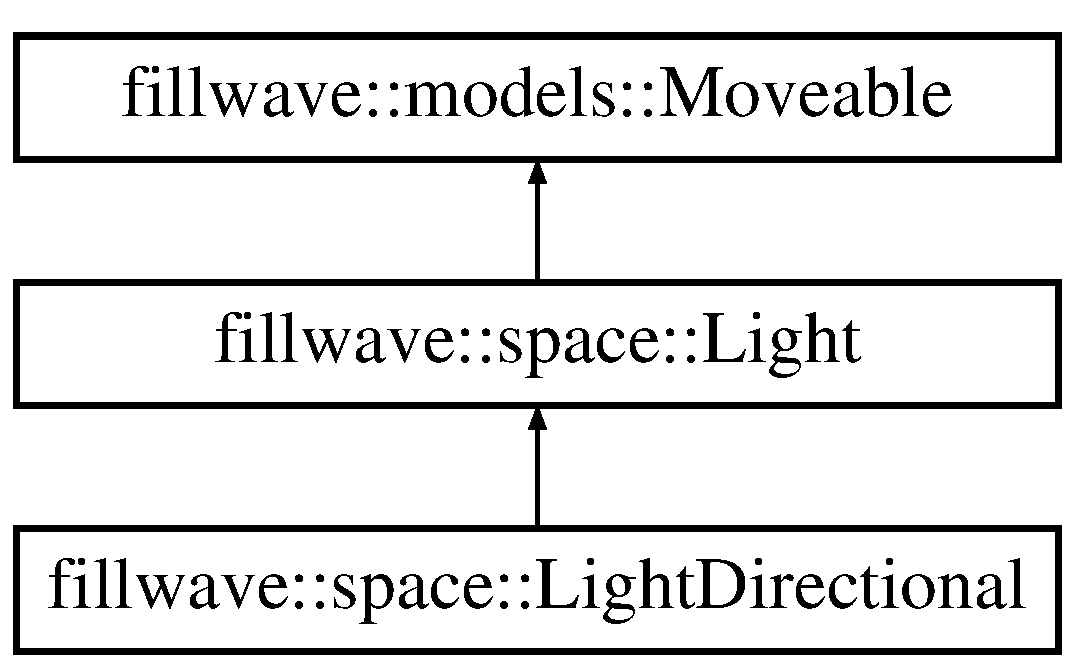
\includegraphics[height=3.000000cm]{classfillwave_1_1space_1_1LightDirectional}
\end{center}
\end{figure}
\subsection*{Public Member Functions}
\begin{DoxyCompactItemize}
\item 
\hypertarget{classfillwave_1_1space_1_1LightDirectional_a4f6accd7aa58e979dcabe1532bd95016}{}{\bfseries Light\+Directional} (p\+Texture2\+D\+Renderable shadow\+Texture, glm\+::vec3 position, glm\+::quat rotation, glm\+::vec4 intensity, p\+Entity entity)\label{classfillwave_1_1space_1_1LightDirectional_a4f6accd7aa58e979dcabe1532bd95016}

\item 
\hypertarget{classfillwave_1_1space_1_1LightDirectional_a801985b17319191c36001565247a3a8e}{}p\+Texture2\+D\+Renderable {\bfseries get\+Shadow\+Texture} ()\label{classfillwave_1_1space_1_1LightDirectional_a801985b17319191c36001565247a3a8e}

\item 
\hypertarget{classfillwave_1_1space_1_1LightDirectional_ac8197dc1c53f12e3e857f1a536183f97}{}p\+Camera\+Orthographic {\bfseries get\+Shadow\+Camera} ()\label{classfillwave_1_1space_1_1LightDirectional_ac8197dc1c53f12e3e857f1a536183f97}

\item 
\hypertarget{classfillwave_1_1space_1_1LightDirectional_a639ebf20be0d085c5d29dedff5cb9cfa}{}void {\bfseries update\+Shadow\+Camera} ()\label{classfillwave_1_1space_1_1LightDirectional_a639ebf20be0d085c5d29dedff5cb9cfa}

\item 
\hypertarget{classfillwave_1_1space_1_1LightDirectional_add38e17785c8a66ffbb2a2af067f0a80}{}void {\bfseries log} ()\label{classfillwave_1_1space_1_1LightDirectional_add38e17785c8a66ffbb2a2af067f0a80}

\end{DoxyCompactItemize}
\subsection*{Additional Inherited Members}


\subsection{Detailed Description}
\hyperlink{classfillwave_1_1space_1_1Light}{Light} with Orthographic projection. 

The documentation for this class was generated from the following file\+:\begin{DoxyCompactItemize}
\item 
/home/filip/\+Projects/fillwave/inc/fillwave/space/Light\+Directional.\+h\end{DoxyCompactItemize}

\hypertarget{classfillwave_1_1manager_1_1LightManager}{}\section{fillwave\+:\+:manager\+:\+:Light\+Manager Class Reference}
\label{classfillwave_1_1manager_1_1LightManager}\index{fillwave\+::manager\+::\+Light\+Manager@{fillwave\+::manager\+::\+Light\+Manager}}


Manager to handle Light objects.  




{\ttfamily \#include $<$Light\+Manager.\+h$>$}

\subsection*{Public Member Functions}
\begin{DoxyCompactItemize}
\item 
\hypertarget{classfillwave_1_1manager_1_1LightManager_a4b7977b87006efcdf07618de5acad752}{}{\bfseries Light\+Manager} (G\+Lsizei screen\+Width, G\+Lsizei screen\+Height)\label{classfillwave_1_1manager_1_1LightManager_a4b7977b87006efcdf07618de5acad752}

\item 
\hypertarget{classfillwave_1_1manager_1_1LightManager_a2283c6285ffa221a603ee05ec22347c5}{}G\+Lboolean {\bfseries is\+Lights\+Refresh} ()\label{classfillwave_1_1manager_1_1LightManager_a2283c6285ffa221a603ee05ec22347c5}

\item 
\hypertarget{classfillwave_1_1manager_1_1LightManager_a391b17400c552e9efb93a2a2a935c758}{}void {\bfseries reset\+Lights\+Refresh} ()\label{classfillwave_1_1manager_1_1LightManager_a391b17400c552e9efb93a2a2a935c758}

\item 
\hypertarget{classfillwave_1_1manager_1_1LightManager_a96c90203d0cfc1582ee6c56397ac3c8a}{}{\footnotesize template$<$class T $>$ }\\G\+Lboolean {\bfseries is\+Refresh\+Light} (std\+::vector$<$ T $>$ \&data)\label{classfillwave_1_1manager_1_1LightManager_a96c90203d0cfc1582ee6c56397ac3c8a}

\item 
\hypertarget{classfillwave_1_1manager_1_1LightManager_a6a4ac44033da265c712b33d35e3e30c9}{}{\footnotesize template$<$class T $>$ }\\void {\bfseries reset\+Refresh\+Light} (std\+::vector$<$ T $>$ \&data)\label{classfillwave_1_1manager_1_1LightManager_a6a4ac44033da265c712b33d35e3e30c9}

\item 
\hypertarget{classfillwave_1_1manager_1_1LightManager_a10802189a60a56d7da8ab19218455ade}{}p\+Light\+Spot {\bfseries add\+Light\+Spot} (p\+Texture2\+D\+Renderable shadow\+Texture, glm\+::vec3 position, glm\+::quat rotation, glm\+::vec4 color, p\+Entity entity=p\+Entity())\label{classfillwave_1_1manager_1_1LightManager_a10802189a60a56d7da8ab19218455ade}

\item 
\hypertarget{classfillwave_1_1manager_1_1LightManager_a65b9b3710d15f835347558ec1d0c68c6}{}p\+Light\+Point {\bfseries add\+Light\+Point} (p\+Texture3\+D\+Renderable shadow\+Texture, glm\+::vec3 position, glm\+::vec4 intensity, p\+Entity entity)\label{classfillwave_1_1manager_1_1LightManager_a65b9b3710d15f835347558ec1d0c68c6}

\item 
\hypertarget{classfillwave_1_1manager_1_1LightManager_abd846f37d19c66fcccb8c3fef76e5a06}{}p\+Light\+Directional {\bfseries add\+Light\+Directional} (p\+Texture2\+D\+Renderable shadow\+Texture, glm\+::vec3 position, glm\+::quat rotation, glm\+::vec4 color, p\+Entity entity=p\+Entity())\label{classfillwave_1_1manager_1_1LightManager_abd846f37d19c66fcccb8c3fef76e5a06}

\item 
\hypertarget{classfillwave_1_1manager_1_1LightManager_afe5d317d70f4bd4e7fd31a4d68b69166}{}void {\bfseries remove\+Light} (p\+Light\+Spot light)\label{classfillwave_1_1manager_1_1LightManager_afe5d317d70f4bd4e7fd31a4d68b69166}

\item 
\hypertarget{classfillwave_1_1manager_1_1LightManager_aae119dab78760bb24ed56eb084108b16}{}void {\bfseries remove\+Light} (p\+Light\+Directional light)\label{classfillwave_1_1manager_1_1LightManager_aae119dab78760bb24ed56eb084108b16}

\item 
\hypertarget{classfillwave_1_1manager_1_1LightManager_aab8ddf66550290c5b0ac36d81625d9bf}{}void {\bfseries remove\+Light} (p\+Light\+Point light)\label{classfillwave_1_1manager_1_1LightManager_aab8ddf66550290c5b0ac36d81625d9bf}

\item 
\hypertarget{classfillwave_1_1manager_1_1LightManager_a5a09a81db30f69598dce305c3e4d3d11}{}void {\bfseries remove\+Lights} ()\label{classfillwave_1_1manager_1_1LightManager_a5a09a81db30f69598dce305c3e4d3d11}

\item 
\hypertarget{classfillwave_1_1manager_1_1LightManager_ac58329c748b34a65aef056a279a6e1ab}{}G\+Lint {\bfseries get\+Lights\+Spot\+How\+Many} ()\label{classfillwave_1_1manager_1_1LightManager_ac58329c748b34a65aef056a279a6e1ab}

\item 
\hypertarget{classfillwave_1_1manager_1_1LightManager_a9b7eaa47f2ba87c99e43dd061ded957c}{}G\+Lint {\bfseries get\+Lights\+Directional\+How\+Many} ()\label{classfillwave_1_1manager_1_1LightManager_a9b7eaa47f2ba87c99e43dd061ded957c}

\item 
\hypertarget{classfillwave_1_1manager_1_1LightManager_ac870410261af76810b8008da28c17cd4}{}G\+Lint {\bfseries get\+Lights\+Point\+How\+Many} ()\label{classfillwave_1_1manager_1_1LightManager_ac870410261af76810b8008da28c17cd4}

\item 
\hypertarget{classfillwave_1_1manager_1_1LightManager_a71ba67dac4b0e50d1e0170245a556c8a}{}void {\bfseries update\+Light\+Entities} ()\label{classfillwave_1_1manager_1_1LightManager_a71ba67dac4b0e50d1e0170245a556c8a}

\item 
\hypertarget{classfillwave_1_1manager_1_1LightManager_a6400031ac36e11f63bc889391370f677}{}void {\bfseries push\+Light\+Uniforms\+D\+R} (\hyperlink{classfillwave_1_1space_1_1Camera}{space\+::\+Camera} \&c, \hyperlink{classfillwave_1_1core_1_1Program}{core\+::\+Program} $\ast$program)\label{classfillwave_1_1manager_1_1LightManager_a6400031ac36e11f63bc889391370f677}

\item 
\hypertarget{classfillwave_1_1manager_1_1LightManager_a4660bf4b9375e971a8b5fef9c0f222d3}{}void {\bfseries push\+Light\+Uniforms} (\hyperlink{classfillwave_1_1space_1_1Camera}{space\+::\+Camera} \&c, \hyperlink{classfillwave_1_1core_1_1Program}{core\+::\+Program} $\ast$program)\label{classfillwave_1_1manager_1_1LightManager_a4660bf4b9375e971a8b5fef9c0f222d3}

\item 
\hypertarget{classfillwave_1_1manager_1_1LightManager_a38547c86c5c918f4f14e2f95ae4c65b7}{}void {\bfseries push\+Light\+Uniform\+Buffers} (\hyperlink{classfillwave_1_1core_1_1Program}{core\+::\+Program} $\ast$program)\label{classfillwave_1_1manager_1_1LightManager_a38547c86c5c918f4f14e2f95ae4c65b7}

\item 
\hypertarget{classfillwave_1_1manager_1_1LightManager_a12236bb6d0781301f3c5987dade6995c}{}void {\bfseries update\+Deferred\+Buffer\+Spot} (G\+Luint light\+I\+D, \hyperlink{classfillwave_1_1core_1_1Program}{core\+::\+Program} $\ast$program, G\+Lint current\+Shadow\+Unit)\label{classfillwave_1_1manager_1_1LightManager_a12236bb6d0781301f3c5987dade6995c}

\item 
\hypertarget{classfillwave_1_1manager_1_1LightManager_a4caeaf8a6af34c192201c17342ca4159}{}void {\bfseries update\+Deferred\+Buffer\+Directional} (G\+Luint light\+I\+D, \hyperlink{classfillwave_1_1core_1_1Program}{core\+::\+Program} $\ast$program, G\+Lint current\+Shadow\+Unit)\label{classfillwave_1_1manager_1_1LightManager_a4caeaf8a6af34c192201c17342ca4159}

\item 
\hypertarget{classfillwave_1_1manager_1_1LightManager_ac1a3eaacb3933a6373b9774a05f5fd61}{}void {\bfseries update\+Deferred\+Buffer\+Point} (G\+Luint light\+I\+D, \hyperlink{classfillwave_1_1core_1_1Program}{core\+::\+Program} $\ast$program, G\+Lint current\+Shadow\+Unit)\label{classfillwave_1_1manager_1_1LightManager_ac1a3eaacb3933a6373b9774a05f5fd61}

\item 
\hypertarget{classfillwave_1_1manager_1_1LightManager_a10eecb05b4cb11f0698abbe8e4c606d2}{}p\+Light\+Spot {\bfseries get\+Light\+Spot} (G\+Lint i)\label{classfillwave_1_1manager_1_1LightManager_a10eecb05b4cb11f0698abbe8e4c606d2}

\item 
\hypertarget{classfillwave_1_1manager_1_1LightManager_a6ce352a65f9dd327e026b875786e3789}{}p\+Light\+Point {\bfseries get\+Light\+Point} (G\+Lint i)\label{classfillwave_1_1manager_1_1LightManager_a6ce352a65f9dd327e026b875786e3789}

\item 
\hypertarget{classfillwave_1_1manager_1_1LightManager_a4c76231b20a196bc20f0ed6fe4625a85}{}p\+Light\+Directional {\bfseries get\+Light\+Directional} (G\+Lint i)\label{classfillwave_1_1manager_1_1LightManager_a4c76231b20a196bc20f0ed6fe4625a85}

\item 
\hypertarget{classfillwave_1_1manager_1_1LightManager_a49d6b5f3a34e867a3452960b43ecac1e}{}G\+Lint {\bfseries obtain\+Texture\+Unit} ()\label{classfillwave_1_1manager_1_1LightManager_a49d6b5f3a34e867a3452960b43ecac1e}

\item 
\hypertarget{classfillwave_1_1manager_1_1LightManager_a91946491b51f766a7cd4da73f06eccd3}{}void {\bfseries free\+Texture\+Unit} (G\+Lint id)\label{classfillwave_1_1manager_1_1LightManager_a91946491b51f766a7cd4da73f06eccd3}

\item 
\hypertarget{classfillwave_1_1manager_1_1LightManager_a77fd3a3574765c47fda19c8c4b92f14a}{}void {\bfseries bind\+Shadowmaps} ()\label{classfillwave_1_1manager_1_1LightManager_a77fd3a3574765c47fda19c8c4b92f14a}

\end{DoxyCompactItemize}


\subsection{Detailed Description}
Manager to handle Light objects. 

The documentation for this class was generated from the following file\+:\begin{DoxyCompactItemize}
\item 
/home/filip/\+Projects/fillwave/inc/fillwave/management/Light\+Manager.\+h\end{DoxyCompactItemize}

\hypertarget{classfillwave_1_1space_1_1LightPoint}{}\section{fillwave\+:\+:space\+:\+:Light\+Point Class Reference}
\label{classfillwave_1_1space_1_1LightPoint}\index{fillwave\+::space\+::\+Light\+Point@{fillwave\+::space\+::\+Light\+Point}}


Not used.  




{\ttfamily \#include $<$Light\+Point.\+h$>$}

Inheritance diagram for fillwave\+:\+:space\+:\+:Light\+Point\+:\begin{figure}[H]
\begin{center}
\leavevmode
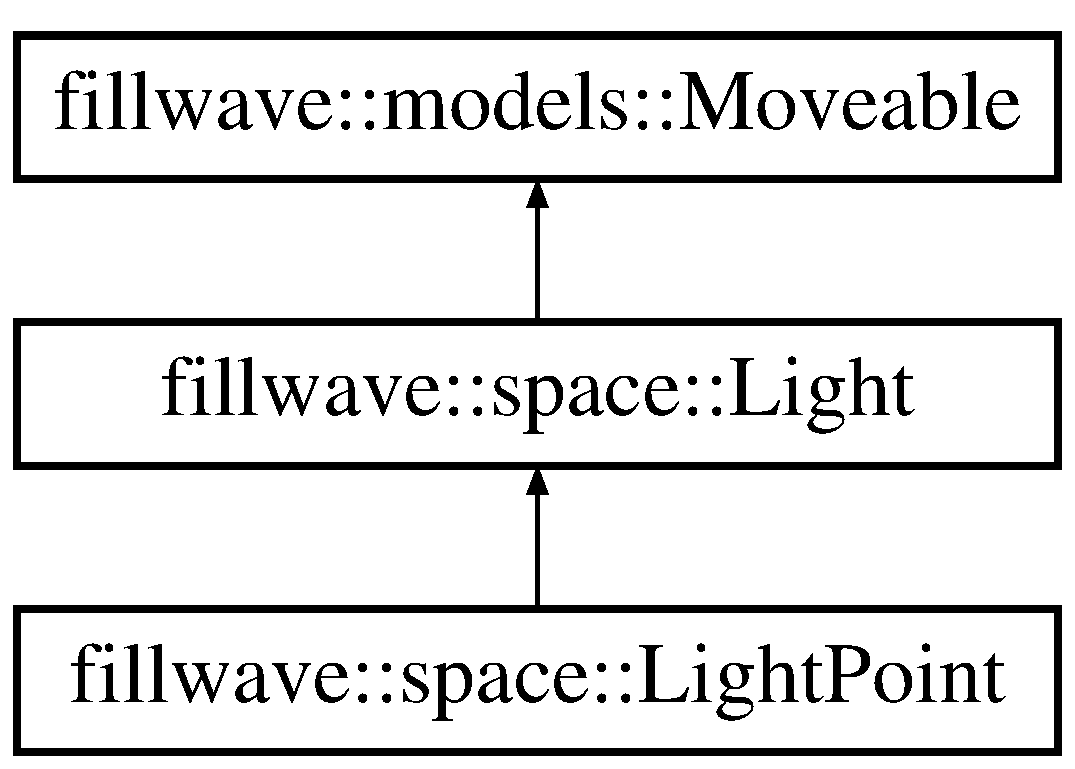
\includegraphics[height=3.000000cm]{classfillwave_1_1space_1_1LightPoint}
\end{center}
\end{figure}
\subsection*{Public Member Functions}
\begin{DoxyCompactItemize}
\item 
\hypertarget{classfillwave_1_1space_1_1LightPoint_a2d5b4c14dc3273997cff3059793f7be0}{}{\bfseries Light\+Point} (p\+Texture3\+D\+Renderable shadow\+Texture, glm\+::vec3 position, glm\+::vec4 intensity, p\+Entity entity=p\+Entity())\label{classfillwave_1_1space_1_1LightPoint_a2d5b4c14dc3273997cff3059793f7be0}

\item 
\hypertarget{classfillwave_1_1space_1_1LightPoint_af37bbbac16a98634bb63f1ec9fb440a2}{}p\+Texture3\+D\+Renderable {\bfseries get\+Shadow\+Texture} ()\label{classfillwave_1_1space_1_1LightPoint_af37bbbac16a98634bb63f1ec9fb440a2}

\item 
\hypertarget{classfillwave_1_1space_1_1LightPoint_a9bb50dbf67e231841556ab11784633a2}{}p\+Camera\+Perspective {\bfseries get\+Shadow\+Camera} (G\+Lenum id)\label{classfillwave_1_1space_1_1LightPoint_a9bb50dbf67e231841556ab11784633a2}

\item 
\hypertarget{classfillwave_1_1space_1_1LightPoint_a5aace7f3a717ffff4e9ba352284cd41c}{}void {\bfseries update\+Shadow\+Camera} ()\label{classfillwave_1_1space_1_1LightPoint_a5aace7f3a717ffff4e9ba352284cd41c}

\item 
\hypertarget{classfillwave_1_1space_1_1LightPoint_ac879a45ce8e5454fcaba8585c4dc1fd1}{}void {\bfseries set\+Entity} (p\+Entity entity)\label{classfillwave_1_1space_1_1LightPoint_ac879a45ce8e5454fcaba8585c4dc1fd1}

\item 
p\+Entity \hyperlink{classfillwave_1_1space_1_1LightPoint_a48f9307245205c1d0cf0a4a7d0fab61e}{get\+Entity} ()
\begin{DoxyCompactList}\small\item\em get the entity assigned to this light \end{DoxyCompactList}\end{DoxyCompactItemize}
\subsection*{Protected Attributes}
\begin{DoxyCompactItemize}
\item 
\hypertarget{classfillwave_1_1space_1_1LightPoint_ac4b938e996e43a388cf7a7dbeb19b5dc}{}p\+Texture3\+D\+Renderable {\bfseries m\+Shadow\+Texture}\label{classfillwave_1_1space_1_1LightPoint_ac4b938e996e43a388cf7a7dbeb19b5dc}

\item 
\hypertarget{classfillwave_1_1space_1_1LightPoint_afe4a22150041b65abf9e140cbe005993}{}std\+::map$<$ G\+Lenum, p\+Camera\+Perspective $>$ {\bfseries m\+Face\+Cameras}\label{classfillwave_1_1space_1_1LightPoint_afe4a22150041b65abf9e140cbe005993}

\end{DoxyCompactItemize}


\subsection{Detailed Description}
Not used. 

\subsection{Member Function Documentation}
\hypertarget{classfillwave_1_1space_1_1LightPoint_a48f9307245205c1d0cf0a4a7d0fab61e}{}\index{fillwave\+::space\+::\+Light\+Point@{fillwave\+::space\+::\+Light\+Point}!get\+Entity@{get\+Entity}}
\index{get\+Entity@{get\+Entity}!fillwave\+::space\+::\+Light\+Point@{fillwave\+::space\+::\+Light\+Point}}
\subsubsection[{get\+Entity}]{\setlength{\rightskip}{0pt plus 5cm}p\+Entity fillwave\+::space\+::\+Light\+Point\+::get\+Entity (
\begin{DoxyParamCaption}
{}
\end{DoxyParamCaption}
)}\label{classfillwave_1_1space_1_1LightPoint_a48f9307245205c1d0cf0a4a7d0fab61e}


get the entity assigned to this light 

get\+Entity 

The documentation for this class was generated from the following file\+:\begin{DoxyCompactItemize}
\item 
/home/filip/\+Projects/fillwave/inc/fillwave/space/Light\+Point.\+h\end{DoxyCompactItemize}

\hypertarget{classfillwave_1_1space_1_1LightSpot}{}\section{fillwave\+:\+:space\+:\+:Light\+Spot Class Reference}
\label{classfillwave_1_1space_1_1LightSpot}\index{fillwave\+::space\+::\+Light\+Spot@{fillwave\+::space\+::\+Light\+Spot}}


\hyperlink{classfillwave_1_1space_1_1Light}{Light} implementing directional torch.  




{\ttfamily \#include $<$Light\+Spot.\+h$>$}

Inheritance diagram for fillwave\+:\+:space\+:\+:Light\+Spot\+:\begin{figure}[H]
\begin{center}
\leavevmode
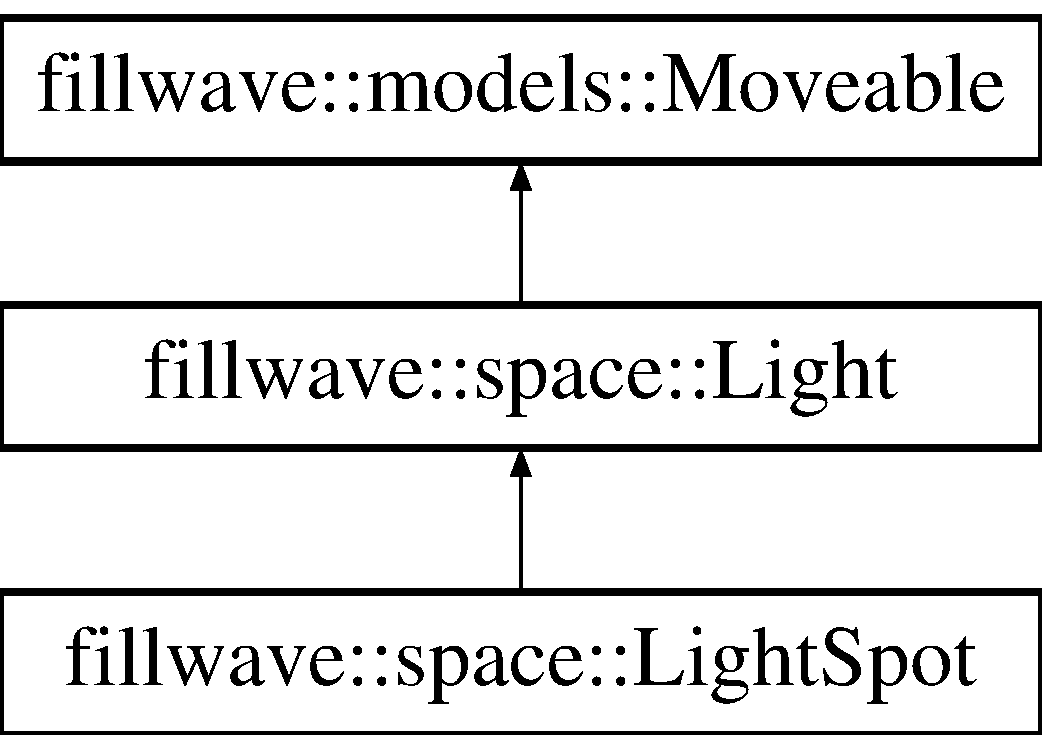
\includegraphics[height=3.000000cm]{classfillwave_1_1space_1_1LightSpot}
\end{center}
\end{figure}
\subsection*{Public Member Functions}
\begin{DoxyCompactItemize}
\item 
\hypertarget{classfillwave_1_1space_1_1LightSpot_ad2de5a9d21cb29127bb2a6a13f0cda05}{}{\bfseries Light\+Spot} (p\+Texture2\+D\+Renderable shadow\+Texture, glm\+::vec3 position, glm\+::quat rotation, glm\+::vec4 intensity, p\+Entity entity=p\+Entity())\label{classfillwave_1_1space_1_1LightSpot_ad2de5a9d21cb29127bb2a6a13f0cda05}

\item 
\hypertarget{classfillwave_1_1space_1_1LightSpot_ac5ccc0c95e9ea3450a321cacd74d29c2}{}p\+Texture2\+D\+Renderable {\bfseries get\+Shadow\+Texture} ()\label{classfillwave_1_1space_1_1LightSpot_ac5ccc0c95e9ea3450a321cacd74d29c2}

\item 
\hypertarget{classfillwave_1_1space_1_1LightSpot_a70b3b4e8742f171c0e4d08dd7ef3cc39}{}p\+Camera\+Perspective {\bfseries get\+Shadow\+Camera} ()\label{classfillwave_1_1space_1_1LightSpot_a70b3b4e8742f171c0e4d08dd7ef3cc39}

\item 
\hypertarget{classfillwave_1_1space_1_1LightSpot_a316a1eba3b245a9d961c4f89bd6a68b6}{}void {\bfseries update\+Shadow\+Camera} ()\label{classfillwave_1_1space_1_1LightSpot_a316a1eba3b245a9d961c4f89bd6a68b6}

\item 
\hypertarget{classfillwave_1_1space_1_1LightSpot_a71982dc9a709282f04b8bf52702f0877}{}void {\bfseries log} ()\label{classfillwave_1_1space_1_1LightSpot_a71982dc9a709282f04b8bf52702f0877}

\end{DoxyCompactItemize}
\subsection*{Protected Attributes}
\begin{DoxyCompactItemize}
\item 
\hypertarget{classfillwave_1_1space_1_1LightSpot_ac622f73ab05f58ff9780b1918eb5d2cc}{}p\+Camera\+Perspective {\bfseries m\+Shadow\+Camera}\label{classfillwave_1_1space_1_1LightSpot_ac622f73ab05f58ff9780b1918eb5d2cc}

\item 
\hypertarget{classfillwave_1_1space_1_1LightSpot_ac5c8723664455f70d0afffc4ddcdfba5}{}p\+Texture2\+D\+Renderable {\bfseries m\+Shadow\+Texture}\label{classfillwave_1_1space_1_1LightSpot_ac5c8723664455f70d0afffc4ddcdfba5}

\end{DoxyCompactItemize}


\subsection{Detailed Description}
\hyperlink{classfillwave_1_1space_1_1Light}{Light} implementing directional torch. 

The documentation for this class was generated from the following file\+:\begin{DoxyCompactItemize}
\item 
/home/filip/\+Projects/fillwave/inc/fillwave/space/Light\+Spot.\+h\end{DoxyCompactItemize}

\hypertarget{structfillwave_1_1space_1_1LighUniformData}{}\section{fillwave\+:\+:space\+:\+:Ligh\+Uniform\+Data Struct Reference}
\label{structfillwave_1_1space_1_1LighUniformData}\index{fillwave\+::space\+::\+Ligh\+Uniform\+Data@{fillwave\+::space\+::\+Ligh\+Uniform\+Data}}


\hyperlink{classfillwave_1_1space_1_1Light}{Light} U\+B\+O data.  




{\ttfamily \#include $<$Light.\+h$>$}

\subsection*{Public Attributes}
\begin{DoxyCompactItemize}
\item 
\hypertarget{structfillwave_1_1space_1_1LighUniformData_a9bb27c99f96c56eae7c1125162b6b309}{}G\+Lfloat {\bfseries position} \mbox{[}4\mbox{]}\label{structfillwave_1_1space_1_1LighUniformData_a9bb27c99f96c56eae7c1125162b6b309}

\item 
\hypertarget{structfillwave_1_1space_1_1LighUniformData_a9e2ff9c77fcbd7a8a18e21a0cff8a932}{}G\+Lfloat {\bfseries intensity} \mbox{[}4\mbox{]}\label{structfillwave_1_1space_1_1LighUniformData_a9e2ff9c77fcbd7a8a18e21a0cff8a932}

\item 
\hypertarget{structfillwave_1_1space_1_1LighUniformData_aa7ebb496349fe71f7a9c25647bf915ab}{}G\+Lfloat {\bfseries mvp} \mbox{[}16\mbox{]}\label{structfillwave_1_1space_1_1LighUniformData_aa7ebb496349fe71f7a9c25647bf915ab}

\end{DoxyCompactItemize}


\subsection{Detailed Description}
\hyperlink{classfillwave_1_1space_1_1Light}{Light} U\+B\+O data. 

The documentation for this struct was generated from the following file\+:\begin{DoxyCompactItemize}
\item 
/home/filip/\+Projects/fillwave/inc/fillwave/space/Light.\+h\end{DoxyCompactItemize}

\hypertarget{classfillwave_1_1actions_1_1LoopCallback}{}\section{fillwave\+:\+:actions\+:\+:Loop\+Callback Class Reference}
\label{classfillwave_1_1actions_1_1LoopCallback}\index{fillwave\+::actions\+::\+Loop\+Callback@{fillwave\+::actions\+::\+Loop\+Callback}}


\hyperlink{classfillwave_1_1actions_1_1ItemCallback}{Item\+Callback} to loop other callbacks.  




{\ttfamily \#include $<$Loop\+Callback.\+h$>$}

Inheritance diagram for fillwave\+:\+:actions\+:\+:Loop\+Callback\+:\begin{figure}[H]
\begin{center}
\leavevmode
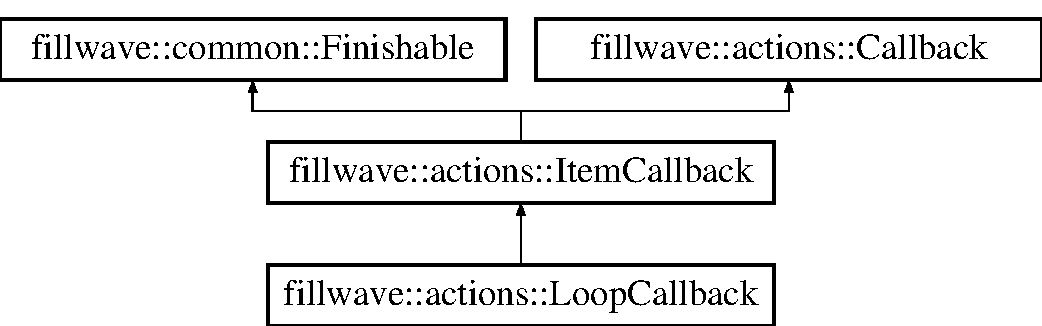
\includegraphics[height=3.000000cm]{classfillwave_1_1actions_1_1LoopCallback}
\end{center}
\end{figure}
\subsection*{Public Member Functions}
\begin{DoxyCompactItemize}
\item 
\hypertarget{classfillwave_1_1actions_1_1LoopCallback_a45b4882a85854a47be1e314c7e9d574b}{}{\bfseries Loop\+Callback} (\hyperlink{classfillwave_1_1actions_1_1ItemCallback}{Item\+Callback} $\ast$callback, int number\+Of\+Executions)\label{classfillwave_1_1actions_1_1LoopCallback_a45b4882a85854a47be1e314c7e9d574b}

\item 
\hypertarget{classfillwave_1_1actions_1_1LoopCallback_ad6f861647fddcd3391d3acc0653f292a}{}void {\bfseries perform} (\hyperlink{classfillwave_1_1actions_1_1EventType}{Event\+Type} $\ast$event)\label{classfillwave_1_1actions_1_1LoopCallback_ad6f861647fddcd3391d3acc0653f292a}

\end{DoxyCompactItemize}
\subsection*{Protected Attributes}
\begin{DoxyCompactItemize}
\item 
\hypertarget{classfillwave_1_1actions_1_1LoopCallback_a41bf4026bd8761dbf0d3912eebf15ad8}{}\hyperlink{classfillwave_1_1actions_1_1ItemCallback}{Item\+Callback} $\ast$ {\bfseries m\+Item\+Callback}\label{classfillwave_1_1actions_1_1LoopCallback_a41bf4026bd8761dbf0d3912eebf15ad8}

\item 
\hypertarget{classfillwave_1_1actions_1_1LoopCallback_abf698e30fc8b93c3459f1739a5ee201f}{}int {\bfseries m\+Loops\+Left}\label{classfillwave_1_1actions_1_1LoopCallback_abf698e30fc8b93c3459f1739a5ee201f}

\end{DoxyCompactItemize}


\subsection{Detailed Description}
\hyperlink{classfillwave_1_1actions_1_1ItemCallback}{Item\+Callback} to loop other callbacks. 

The documentation for this class was generated from the following file\+:\begin{DoxyCompactItemize}
\item 
/home/filip/\+Projects/fillwave/inc/fillwave/actions/Loop\+Callback.\+h\end{DoxyCompactItemize}

\hypertarget{classfillwave_1_1models_1_1Material}{}\section{fillwave\+:\+:models\+:\+:Material Class Reference}
\label{classfillwave_1_1models_1_1Material}\index{fillwave\+::models\+::\+Material@{fillwave\+::models\+::\+Material}}


Per mesh material info.  




{\ttfamily \#include $<$Material.\+h$>$}

\subsection*{Public Member Functions}
\begin{DoxyCompactItemize}
\item 
\hypertarget{classfillwave_1_1models_1_1Material_a4dbd7486f1d41540f7fd1592765765d0}{}{\bfseries Material} (const f\+Material $\ast$material)\label{classfillwave_1_1models_1_1Material_a4dbd7486f1d41540f7fd1592765765d0}

\item 
\hypertarget{classfillwave_1_1models_1_1Material_aac031db0c9f5d1ab1c37118663a498ac}{}glm\+::vec4 {\bfseries get\+Ambient} ()\label{classfillwave_1_1models_1_1Material_aac031db0c9f5d1ab1c37118663a498ac}

\item 
\hypertarget{classfillwave_1_1models_1_1Material_a2b71ceb7691cd4a381b3f12d98faa3ab}{}glm\+::vec4 {\bfseries get\+Diffuse} ()\label{classfillwave_1_1models_1_1Material_a2b71ceb7691cd4a381b3f12d98faa3ab}

\item 
\hypertarget{classfillwave_1_1models_1_1Material_a56e4999872ffccf557a97b3f27bff019}{}glm\+::vec4 {\bfseries get\+Specular} ()\label{classfillwave_1_1models_1_1Material_a56e4999872ffccf557a97b3f27bff019}

\end{DoxyCompactItemize}


\subsection{Detailed Description}
Per mesh material info. 

The documentation for this class was generated from the following file\+:\begin{DoxyCompactItemize}
\item 
/home/filip/\+Projects/fillwave/inc/fillwave/models/Material.\+h\end{DoxyCompactItemize}

\hypertarget{classfillwave_1_1models_1_1Mesh}{}\section{fillwave\+:\+:models\+:\+:Mesh Class Reference}
\label{classfillwave_1_1models_1_1Mesh}\index{fillwave\+::models\+::\+Mesh@{fillwave\+::models\+::\+Mesh}}


Basic drawable \hyperlink{classfillwave_1_1models_1_1Entity}{Entity}.  




{\ttfamily \#include $<$Mesh.\+h$>$}

Inheritance diagram for fillwave\+:\+:models\+:\+:Mesh\+:\begin{figure}[H]
\begin{center}
\leavevmode
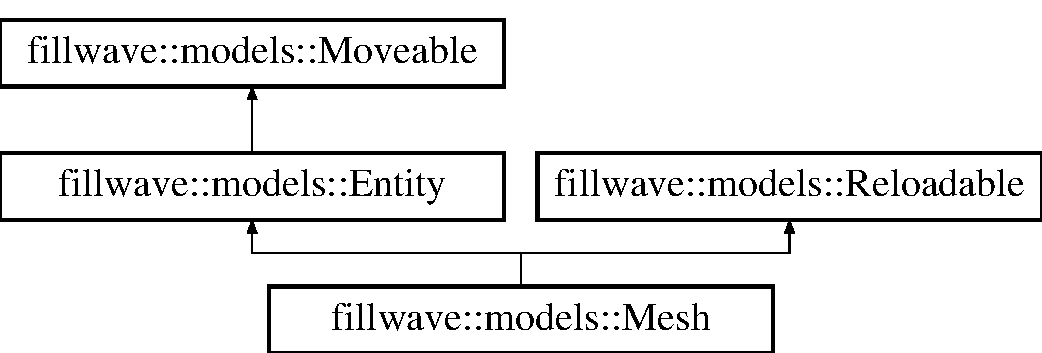
\includegraphics[height=3.000000cm]{classfillwave_1_1models_1_1Mesh}
\end{center}
\end{figure}
\subsection*{Public Member Functions}
\begin{DoxyCompactItemize}
\item 
\hypertarget{classfillwave_1_1models_1_1Mesh_a0d95cbd74a78ef53128f02f7861cee39}{}{\bfseries Mesh} (\hyperlink{classfillwave_1_1Engine}{Engine} $\ast$engine, const \hyperlink{classfillwave_1_1models_1_1Material}{Material} \&material, p\+Texture\+Region diffuse\+Map, p\+Texture\+Region normal\+Map, p\+Texture\+Region specular\+Map, p\+Program program, p\+Program Program\+Shadow, p\+Program program\+Shadow\+Color, p\+Program program\+Occlusion, p\+Program program\+Ambient\+Occlusion\+Geometry, p\+Program program\+Ambient\+Occlusion\+Color, \hyperlink{classfillwave_1_1manager_1_1LightManager}{manager\+::\+Light\+Manager} $\ast$light\+Manager=nullptr, p\+Vertex\+Buffer\+Basic vbo=p\+Vertex\+Buffer\+Basic(), p\+Index\+Buffer\+Basic ibo=p\+Index\+Buffer\+Basic(), \hyperlink{classfillwave_1_1manager_1_1BoneManager}{manager\+::\+Bone\+Manager} $\ast$bone\+Manager=nullptr, G\+Lenum draw\+Type=G\+L\+\_\+\+T\+R\+I\+A\+N\+G\+L\+E\+S)\label{classfillwave_1_1models_1_1Mesh_a0d95cbd74a78ef53128f02f7861cee39}

\item 
\hypertarget{classfillwave_1_1models_1_1Mesh_a90b50f39d7b3c85240bfa4abc109c611}{}virtual void {\bfseries on\+Draw} ()\label{classfillwave_1_1models_1_1Mesh_a90b50f39d7b3c85240bfa4abc109c611}

\item 
\hypertarget{classfillwave_1_1models_1_1Mesh_a2a1b2eba36669467e9565052e2a3bab0}{}void {\bfseries draw} (\hyperlink{classfillwave_1_1space_1_1Camera}{space\+::\+Camera} \&camera)\label{classfillwave_1_1models_1_1Mesh_a2a1b2eba36669467e9565052e2a3bab0}

\item 
\hypertarget{classfillwave_1_1models_1_1Mesh_a5d6f4543c45f5cdb5afed43dfb06efe7}{}void {\bfseries draw\+D\+R} (\hyperlink{classfillwave_1_1space_1_1Camera}{space\+::\+Camera} \&camera)\label{classfillwave_1_1models_1_1Mesh_a5d6f4543c45f5cdb5afed43dfb06efe7}

\item 
\hypertarget{classfillwave_1_1models_1_1Mesh_a06b550cab08ecdf422efcc0f54311804}{}void {\bfseries draw\+Fast} (\hyperlink{classfillwave_1_1space_1_1Camera}{space\+::\+Camera} \&camera)\label{classfillwave_1_1models_1_1Mesh_a06b550cab08ecdf422efcc0f54311804}

\item 
\hypertarget{classfillwave_1_1models_1_1Mesh_a081e7ebcb911584a8fcd6cde9d9f953a}{}void {\bfseries draw\+Picking} (\hyperlink{classfillwave_1_1space_1_1Camera}{space\+::\+Camera} \&camera)\label{classfillwave_1_1models_1_1Mesh_a081e7ebcb911584a8fcd6cde9d9f953a}

\item 
\hypertarget{classfillwave_1_1models_1_1Mesh_a783a7c5c14d82530dab2c8687107f51a}{}void {\bfseries draw\+Depth} (\hyperlink{classfillwave_1_1space_1_1Camera}{space\+::\+Camera} \&camera)\label{classfillwave_1_1models_1_1Mesh_a783a7c5c14d82530dab2c8687107f51a}

\item 
\hypertarget{classfillwave_1_1models_1_1Mesh_a1d8095d0f217c0f48aabc58a50c9d5f2}{}void {\bfseries draw\+Depth\+Color} (\hyperlink{classfillwave_1_1space_1_1Camera}{space\+::\+Camera} \&camera, glm\+::vec3 \&position)\label{classfillwave_1_1models_1_1Mesh_a1d8095d0f217c0f48aabc58a50c9d5f2}

\item 
\hypertarget{classfillwave_1_1models_1_1Mesh_a76dc0c57d61b1d1dd63949080f32a908}{}void {\bfseries draw\+A\+O\+G} (\hyperlink{classfillwave_1_1space_1_1Camera}{space\+::\+Camera} \&camera)\label{classfillwave_1_1models_1_1Mesh_a76dc0c57d61b1d1dd63949080f32a908}

\item 
\hypertarget{classfillwave_1_1models_1_1Mesh_aa17056007b007018db121176a763c40e}{}void {\bfseries draw\+A\+O\+C} (\hyperlink{classfillwave_1_1space_1_1Camera}{space\+::\+Camera} \&camera)\label{classfillwave_1_1models_1_1Mesh_aa17056007b007018db121176a763c40e}

\item 
\hypertarget{classfillwave_1_1models_1_1Mesh_a8ff6fda81a630463470d3adb6d323c07}{}void {\bfseries draw\+Occlusion\+Box} (\hyperlink{classfillwave_1_1space_1_1Camera}{space\+::\+Camera} \&camera)\label{classfillwave_1_1models_1_1Mesh_a8ff6fda81a630463470d3adb6d323c07}

\item 
\hypertarget{classfillwave_1_1models_1_1Mesh_a84c1ebcaddba6386a8eb9e54bf6fd368}{}void {\bfseries log} ()\label{classfillwave_1_1models_1_1Mesh_a84c1ebcaddba6386a8eb9e54bf6fd368}

\end{DoxyCompactItemize}
\subsection*{Protected Attributes}
\begin{DoxyCompactItemize}
\item 
\hypertarget{classfillwave_1_1models_1_1Mesh_ab8b4fb88c0672e5a401539ca768614d8}{}p\+Program {\bfseries m\+Program}\label{classfillwave_1_1models_1_1Mesh_ab8b4fb88c0672e5a401539ca768614d8}

\item 
\hypertarget{classfillwave_1_1models_1_1Mesh_a94aea109e28a2739087a4f231086e188}{}p\+Program {\bfseries m\+Program\+D\+R}\label{classfillwave_1_1models_1_1Mesh_a94aea109e28a2739087a4f231086e188}

\item 
\hypertarget{classfillwave_1_1models_1_1Mesh_aaf192988d408e58260232ef772d9a1ec}{}p\+Program {\bfseries m\+Program\+Shadow}\label{classfillwave_1_1models_1_1Mesh_aaf192988d408e58260232ef772d9a1ec}

\item 
\hypertarget{classfillwave_1_1models_1_1Mesh_aabf7629a9f145489e23a2940852c2e4c}{}p\+Program {\bfseries m\+Program\+Shadow\+Color}\label{classfillwave_1_1models_1_1Mesh_aabf7629a9f145489e23a2940852c2e4c}

\item 
\hypertarget{classfillwave_1_1models_1_1Mesh_a695945e78a10363cf94ec4ba6766051b}{}p\+Program {\bfseries m\+Program\+O\+Q}\label{classfillwave_1_1models_1_1Mesh_a695945e78a10363cf94ec4ba6766051b}

\item 
\hypertarget{classfillwave_1_1models_1_1Mesh_a2be19d4ef719bc8cb09c9cf607b5bda7}{}p\+Program {\bfseries m\+Program\+A\+O\+Geometry}\label{classfillwave_1_1models_1_1Mesh_a2be19d4ef719bc8cb09c9cf607b5bda7}

\item 
\hypertarget{classfillwave_1_1models_1_1Mesh_a995eae1edf0c5d52b5e2b5af8dfe24c3}{}p\+Program {\bfseries m\+Program\+A\+O\+Color}\label{classfillwave_1_1models_1_1Mesh_a995eae1edf0c5d52b5e2b5af8dfe24c3}

\item 
\hypertarget{classfillwave_1_1models_1_1Mesh_a5b11d49699286ff47126c1cdcb620855}{}p\+Texture\+Region {\bfseries m\+Diffuse\+Map}\label{classfillwave_1_1models_1_1Mesh_a5b11d49699286ff47126c1cdcb620855}

\item 
\hypertarget{classfillwave_1_1models_1_1Mesh_a192ce0eeb3e9266a1830ae24faefb693}{}p\+Texture\+Region {\bfseries m\+Normal\+Map}\label{classfillwave_1_1models_1_1Mesh_a192ce0eeb3e9266a1830ae24faefb693}

\item 
\hypertarget{classfillwave_1_1models_1_1Mesh_a700687871870a4c0ba820f408cb2b6b6}{}p\+Texture\+Region {\bfseries m\+Specular\+Map}\label{classfillwave_1_1models_1_1Mesh_a700687871870a4c0ba820f408cb2b6b6}

\item 
\hypertarget{classfillwave_1_1models_1_1Mesh_a392a5802280eebb7cd069adaeada7e51}{}\hyperlink{classfillwave_1_1models_1_1Material}{Material} {\bfseries m\+Material}\label{classfillwave_1_1models_1_1Mesh_a392a5802280eebb7cd069adaeada7e51}

\item 
\hypertarget{classfillwave_1_1models_1_1Mesh_a29aae8348fca2c3af20627cc32753d45}{}G\+Lenum {\bfseries m\+Draw\+Type}\label{classfillwave_1_1models_1_1Mesh_a29aae8348fca2c3af20627cc32753d45}

\item 
\hypertarget{classfillwave_1_1models_1_1Mesh_aa248c623a0240357fb570f597ec887e8}{}\hyperlink{classfillwave_1_1manager_1_1LightManager}{manager\+::\+Light\+Manager} $\ast$ {\bfseries m\+Light\+Manager}\label{classfillwave_1_1models_1_1Mesh_aa248c623a0240357fb570f597ec887e8}

\item 
\hypertarget{classfillwave_1_1models_1_1Mesh_a6ddceb8f803506cdad497150b1c9ad6b}{}\hyperlink{classfillwave_1_1manager_1_1BoneManager}{manager\+::\+Bone\+Manager} $\ast$ {\bfseries m\+Bone\+Manager}\label{classfillwave_1_1models_1_1Mesh_a6ddceb8f803506cdad497150b1c9ad6b}

\item 
\hypertarget{classfillwave_1_1models_1_1Mesh_a1648a98dd8ecfb334b28f4373026340a}{}p\+Vertex\+Buffer\+Basic {\bfseries m\+V\+B\+O}\label{classfillwave_1_1models_1_1Mesh_a1648a98dd8ecfb334b28f4373026340a}

\item 
\hypertarget{classfillwave_1_1models_1_1Mesh_ac05e58d20a10f788af83d4e34bc361fc}{}glm\+::mat4 {\bfseries m\+Occlusion\+Matrix}\label{classfillwave_1_1models_1_1Mesh_ac05e58d20a10f788af83d4e34bc361fc}

\item 
\hypertarget{classfillwave_1_1models_1_1Mesh_a0e8df1a505bdb0286b222d53cf1b301a}{}p\+Index\+Buffer\+Basic {\bfseries m\+I\+B\+O}\label{classfillwave_1_1models_1_1Mesh_a0e8df1a505bdb0286b222d53cf1b301a}

\item 
\hypertarget{classfillwave_1_1models_1_1Mesh_a7cbc0f8fbacfb9dd3d080109ece238b6}{}\hyperlink{classfillwave_1_1core_1_1Query}{core\+::\+Query\+If\+Any\+Samples\+Passed} {\bfseries m\+Occlusion\+Query}\label{classfillwave_1_1models_1_1Mesh_a7cbc0f8fbacfb9dd3d080109ece238b6}

\item 
\hypertarget{classfillwave_1_1models_1_1Mesh_ab734d8c3ec4e7b8e08aca65b49c9c73f}{}\hyperlink{classfillwave_1_1core_1_1ConditionalRender}{core\+::\+Conditional\+Render} {\bfseries m\+Conditional\+Rendering}\label{classfillwave_1_1models_1_1Mesh_ab734d8c3ec4e7b8e08aca65b49c9c73f}

\end{DoxyCompactItemize}


\subsection{Detailed Description}
Basic drawable \hyperlink{classfillwave_1_1models_1_1Entity}{Entity}. 

The documentation for this class was generated from the following file\+:\begin{DoxyCompactItemize}
\item 
/home/filip/\+Projects/fillwave/inc/fillwave/models/Mesh.\+h\end{DoxyCompactItemize}

\hypertarget{classfillwave_1_1terrain_1_1MeshTerrain}{}\section{fillwave\+:\+:terrain\+:\+:Mesh\+Terrain Class Reference}
\label{classfillwave_1_1terrain_1_1MeshTerrain}\index{fillwave\+::terrain\+::\+Mesh\+Terrain@{fillwave\+::terrain\+::\+Mesh\+Terrain}}


Programmable to provide mesh terrain functionality.  




{\ttfamily \#include $<$Mesh\+Terrain.\+h$>$}

Inheritance diagram for fillwave\+:\+:terrain\+:\+:Mesh\+Terrain\+:\begin{figure}[H]
\begin{center}
\leavevmode
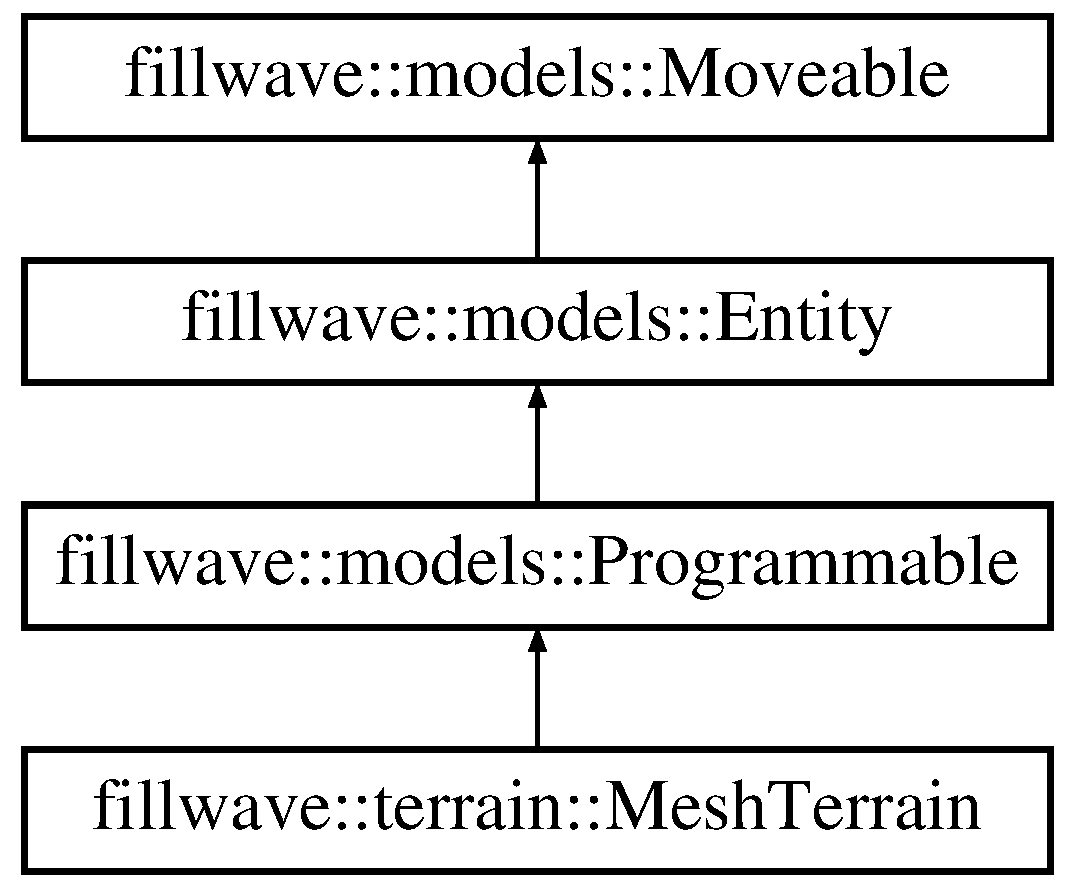
\includegraphics[height=4.000000cm]{classfillwave_1_1terrain_1_1MeshTerrain}
\end{center}
\end{figure}
\subsection*{Public Member Functions}
\begin{DoxyCompactItemize}
\item 
\hypertarget{classfillwave_1_1terrain_1_1MeshTerrain_a99c353aa895746c227ac17233ded6827}{}{\bfseries Mesh\+Terrain} (\hyperlink{classfillwave_1_1Engine}{Engine} $\ast$engine, p\+Program program, \hyperlink{classfillwave_1_1terrain_1_1TerrainConstructor}{terrain\+::\+Terrain\+Constructor} $\ast$constructor, const \hyperlink{classfillwave_1_1models_1_1Material}{models\+::\+Material} \&material, const std\+::string \&diffuse\+Map\+Path, const std\+::string \&normal\+Map\+Path, const std\+::string \&specular\+Map\+Path, G\+Luint radius, G\+Luint density=8)\label{classfillwave_1_1terrain_1_1MeshTerrain_a99c353aa895746c227ac17233ded6827}

\item 
\hypertarget{classfillwave_1_1terrain_1_1MeshTerrain_a43c39831c3a77fc391e0716b3e595533}{}void {\bfseries draw} (\hyperlink{classfillwave_1_1space_1_1Camera}{space\+::\+Camera} \&camera)\label{classfillwave_1_1terrain_1_1MeshTerrain_a43c39831c3a77fc391e0716b3e595533}

\end{DoxyCompactItemize}
\subsection*{Additional Inherited Members}


\subsection{Detailed Description}
Programmable to provide mesh terrain functionality. 

The documentation for this class was generated from the following file\+:\begin{DoxyCompactItemize}
\item 
/home/filip/\+Projects/fillwave/inc/fillwave/terrain/Mesh\+Terrain.\+h\end{DoxyCompactItemize}

\hypertarget{classfillwave_1_1models_1_1Model}{}\section{fillwave\+:\+:models\+:\+:Model Class Reference}
\label{classfillwave_1_1models_1_1Model}\index{fillwave\+::models\+::\+Model@{fillwave\+::models\+::\+Model}}


Drawable \hyperlink{classfillwave_1_1models_1_1Mesh}{Mesh} set.  




{\ttfamily \#include $<$Model.\+h$>$}

Inheritance diagram for fillwave\+:\+:models\+:\+:Model\+:\begin{figure}[H]
\begin{center}
\leavevmode
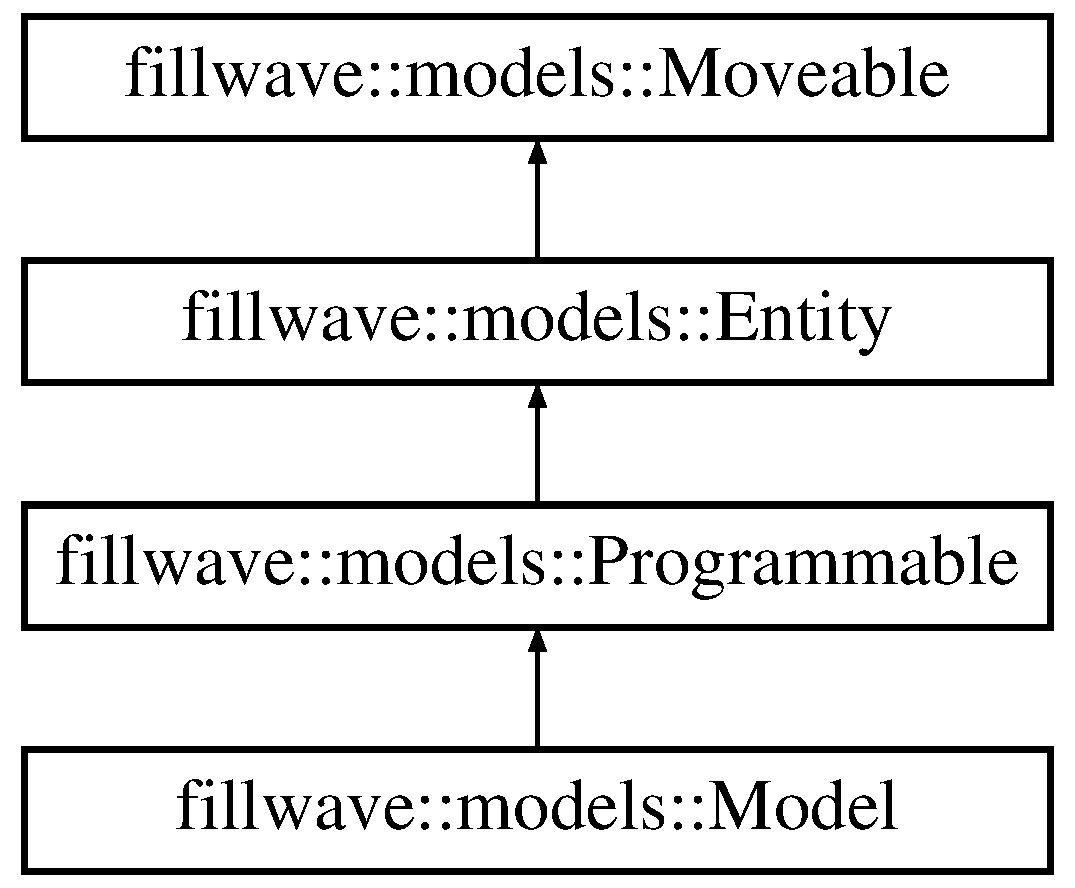
\includegraphics[height=4.000000cm]{classfillwave_1_1models_1_1Model}
\end{center}
\end{figure}
\subsection*{Public Member Functions}
\begin{DoxyCompactItemize}
\item 
\hypertarget{classfillwave_1_1models_1_1Model_a5df801152c40789eca8e714d5c66ef38}{}{\bfseries Model} (\hyperlink{classfillwave_1_1Engine}{Engine} $\ast$engine, p\+Program program, \hyperlink{classfillwave_1_1models_1_1Shape}{Shape}$<$ \hyperlink{structfillwave_1_1core_1_1VertexBasic}{core\+::\+Vertex\+Basic} $>$ \&shape, p\+Texture diffuse\+Map, p\+Texture normal\+Map, p\+Texture specular\+Map, const \hyperlink{classfillwave_1_1models_1_1Material}{Material} \&material)\label{classfillwave_1_1models_1_1Model_a5df801152c40789eca8e714d5c66ef38}

\item 
\hypertarget{classfillwave_1_1models_1_1Model_adc746edb80df0da6a33e108bcd860e95}{}{\bfseries Model} (\hyperlink{classfillwave_1_1Engine}{Engine} $\ast$engine, p\+Program program, const std\+::string \&shape\+Path)\label{classfillwave_1_1models_1_1Model_adc746edb80df0da6a33e108bcd860e95}

\item 
\hypertarget{classfillwave_1_1models_1_1Model_aafd17810b12882bade01cdb51267be56}{}{\bfseries Model} (\hyperlink{classfillwave_1_1Engine}{Engine} $\ast$engine, p\+Program program, const std\+::string \&shape\+Path, const std\+::string \&diffuse\+Map\+Path, const std\+::string \&normal\+Map\+Path=\char`\"{}\char`\"{}, const std\+::string \&specular\+Map\+Path=\char`\"{}\char`\"{})\label{classfillwave_1_1models_1_1Model_aafd17810b12882bade01cdb51267be56}

\item 
\hypertarget{classfillwave_1_1models_1_1Model_a763c550189ed4cb8bd3fa7ca09ee8de9}{}{\bfseries Model} (\hyperlink{classfillwave_1_1Engine}{Engine} $\ast$engine, p\+Program program, const std\+::string \&shape\+Path, p\+Texture diffuse\+Map, p\+Texture normal\+Map=p\+Texture(), p\+Texture specular\+Map=p\+Texture(), const \hyperlink{classfillwave_1_1models_1_1Material}{Material} \&material=\hyperlink{classfillwave_1_1models_1_1Material}{Material}())\label{classfillwave_1_1models_1_1Model_a763c550189ed4cb8bd3fa7ca09ee8de9}

\item 
\hypertarget{classfillwave_1_1models_1_1Model_abe4723be91d2b4af304bdc8c36268266}{}void {\bfseries reload} ()\label{classfillwave_1_1models_1_1Model_abe4723be91d2b4af304bdc8c36268266}

\item 
\hypertarget{classfillwave_1_1models_1_1Model_ab1ebb95a646e4b84f74ddc3d320e5aab}{}void {\bfseries draw} (\hyperlink{classfillwave_1_1space_1_1Camera}{space\+::\+Camera} \&camera)\label{classfillwave_1_1models_1_1Model_ab1ebb95a646e4b84f74ddc3d320e5aab}

\item 
\hypertarget{classfillwave_1_1models_1_1Model_adeecb113ec1a7635ce1aa1f2b4a9fc3b}{}void {\bfseries draw\+D\+R} (\hyperlink{classfillwave_1_1space_1_1Camera}{space\+::\+Camera} \&camera)\label{classfillwave_1_1models_1_1Model_adeecb113ec1a7635ce1aa1f2b4a9fc3b}

\item 
\hypertarget{classfillwave_1_1models_1_1Model_aaed476d8c55b45779f874fbe64eb9528}{}void {\bfseries perform\+Animation} (G\+Lfloat time\+Elapsed\+\_\+us)\label{classfillwave_1_1models_1_1Model_aaed476d8c55b45779f874fbe64eb9528}

\item 
\hypertarget{classfillwave_1_1models_1_1Model_a16dee2d4aaf0a44232b84b1a57010e75}{}void {\bfseries set\+Active\+Animation} (G\+Lint animation\+I\+D)\label{classfillwave_1_1models_1_1Model_a16dee2d4aaf0a44232b84b1a57010e75}

\item 
\hypertarget{classfillwave_1_1models_1_1Model_a3af33b02d50e89730d4b8b083d958d61}{}G\+Lint {\bfseries get\+Active\+Animations} ()\label{classfillwave_1_1models_1_1Model_a3af33b02d50e89730d4b8b083d958d61}

\item 
\hypertarget{classfillwave_1_1models_1_1Model_abb9ea989aa1ff7469cebcc9ab62f306d}{}void {\bfseries log} ()\label{classfillwave_1_1models_1_1Model_abb9ea989aa1ff7469cebcc9ab62f306d}

\end{DoxyCompactItemize}
\subsection*{Protected Attributes}
\begin{DoxyCompactItemize}
\item 
\hypertarget{classfillwave_1_1models_1_1Model_aceb3b31dc49c147f290e703c08778627}{}\hyperlink{classfillwave_1_1manager_1_1BoneManager}{manager\+::\+Bone\+Manager} $\ast$ {\bfseries m\+Bone\+Manager}\label{classfillwave_1_1models_1_1Model_aceb3b31dc49c147f290e703c08778627}

\item 
\hypertarget{classfillwave_1_1models_1_1Model_ae7620f5540fc9f44474a7309febdd7fd}{}p\+Program {\bfseries m\+Program\+Shadow}\label{classfillwave_1_1models_1_1Model_ae7620f5540fc9f44474a7309febdd7fd}

\item 
\hypertarget{classfillwave_1_1models_1_1Model_ac1f6861cdf76ae7cd9fb87bc3c306f50}{}p\+Program {\bfseries m\+Program\+Shadow\+Color}\label{classfillwave_1_1models_1_1Model_ac1f6861cdf76ae7cd9fb87bc3c306f50}

\item 
\hypertarget{classfillwave_1_1models_1_1Model_af4e1583c66011ec32e8b4d9bffe62e4f}{}G\+Lint {\bfseries m\+Uniform\+Location\+Cache\+Bones}\label{classfillwave_1_1models_1_1Model_af4e1583c66011ec32e8b4d9bffe62e4f}

\item 
\hypertarget{classfillwave_1_1models_1_1Model_aa30e51157265b3520108dd659e63520e}{}G\+Lint {\bfseries m\+Uniform\+Location\+Cache\+Bones\+Shadow}\label{classfillwave_1_1models_1_1Model_aa30e51157265b3520108dd659e63520e}

\item 
\hypertarget{classfillwave_1_1models_1_1Model_a865e04f17029cab4f3a4175fce30be7a}{}G\+Lint {\bfseries m\+Uniform\+Location\+Cache\+Bones\+Shadow\+Color}\label{classfillwave_1_1models_1_1Model_a865e04f17029cab4f3a4175fce30be7a}

\end{DoxyCompactItemize}


\subsection{Detailed Description}
Drawable \hyperlink{classfillwave_1_1models_1_1Mesh}{Mesh} set. 

The documentation for this class was generated from the following file\+:\begin{DoxyCompactItemize}
\item 
/home/filip/\+Projects/fillwave/inc/fillwave/models/Model.\+h\end{DoxyCompactItemize}

\hypertarget{classfillwave_1_1actions_1_1MouseButtonEvent}{}\section{fillwave\+:\+:actions\+:\+:Mouse\+Button\+Event Class Reference}
\label{classfillwave_1_1actions_1_1MouseButtonEvent}\index{fillwave\+::actions\+::\+Mouse\+Button\+Event@{fillwave\+::actions\+::\+Mouse\+Button\+Event}}


\hyperlink{classfillwave_1_1actions_1_1Event}{Event} introduced when something happens with the mouse buttons.  




{\ttfamily \#include $<$Mouse\+Button\+Event.\+h$>$}

Inheritance diagram for fillwave\+:\+:actions\+:\+:Mouse\+Button\+Event\+:\begin{figure}[H]
\begin{center}
\leavevmode
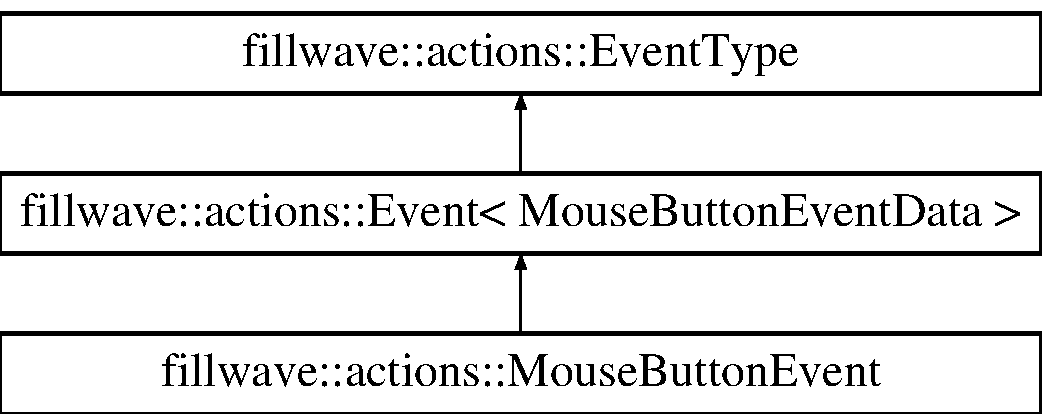
\includegraphics[height=3.000000cm]{classfillwave_1_1actions_1_1MouseButtonEvent}
\end{center}
\end{figure}
\subsection*{Public Member Functions}
\begin{DoxyCompactItemize}
\item 
\hypertarget{classfillwave_1_1actions_1_1MouseButtonEvent_a07a91e9d24b83c49cea27a6952813362}{}{\bfseries Mouse\+Button\+Event} (\hyperlink{structfillwave_1_1actions_1_1MouseButtonEventData}{Mouse\+Button\+Event\+Data} data)\label{classfillwave_1_1actions_1_1MouseButtonEvent_a07a91e9d24b83c49cea27a6952813362}

\end{DoxyCompactItemize}
\subsection*{Additional Inherited Members}


\subsection{Detailed Description}
\hyperlink{classfillwave_1_1actions_1_1Event}{Event} introduced when something happens with the mouse buttons. 

The documentation for this class was generated from the following file\+:\begin{DoxyCompactItemize}
\item 
/home/filip/\+Projects/fillwave/inc/fillwave/actions/Mouse\+Button\+Event.\+h\end{DoxyCompactItemize}

\hypertarget{structfillwave_1_1actions_1_1MouseButtonEventData}{}\section{fillwave\+:\+:actions\+:\+:Mouse\+Button\+Event\+Data Struct Reference}
\label{structfillwave_1_1actions_1_1MouseButtonEventData}\index{fillwave\+::actions\+::\+Mouse\+Button\+Event\+Data@{fillwave\+::actions\+::\+Mouse\+Button\+Event\+Data}}


\hyperlink{classfillwave_1_1actions_1_1Event}{Event} data structure to store the parameters of a button press event.  




{\ttfamily \#include $<$Mouse\+Button\+Event.\+h$>$}

\subsection*{Public Attributes}
\begin{DoxyCompactItemize}
\item 
\hypertarget{structfillwave_1_1actions_1_1MouseButtonEventData_a44dbb23e004b5b8f5a411f3752c22110}{}float {\bfseries m\+Where\+X}\label{structfillwave_1_1actions_1_1MouseButtonEventData_a44dbb23e004b5b8f5a411f3752c22110}

\item 
\hypertarget{structfillwave_1_1actions_1_1MouseButtonEventData_a2336cde2f980612c1980c3bb497838a3}{}float {\bfseries m\+Where\+Y}\label{structfillwave_1_1actions_1_1MouseButtonEventData_a2336cde2f980612c1980c3bb497838a3}

\item 
\hypertarget{structfillwave_1_1actions_1_1MouseButtonEventData_acab5f09b71ea47dd1a89686e5a011505}{}int {\bfseries m\+Button}\label{structfillwave_1_1actions_1_1MouseButtonEventData_acab5f09b71ea47dd1a89686e5a011505}

\item 
\hypertarget{structfillwave_1_1actions_1_1MouseButtonEventData_a39f005f4a802cab2835610fd00c882d9}{}int {\bfseries m\+Action}\label{structfillwave_1_1actions_1_1MouseButtonEventData_a39f005f4a802cab2835610fd00c882d9}

\item 
\hypertarget{structfillwave_1_1actions_1_1MouseButtonEventData_a0dd7a2db4f86c9aed6967c7930689144}{}int {\bfseries m\+Mods}\label{structfillwave_1_1actions_1_1MouseButtonEventData_a0dd7a2db4f86c9aed6967c7930689144}

\item 
\hypertarget{structfillwave_1_1actions_1_1MouseButtonEventData_abd86614b8765b9930160c728bac4f790}{}const e\+Event\+Type {\bfseries type} = e\+Event\+Type\+::mouse\+Button\label{structfillwave_1_1actions_1_1MouseButtonEventData_abd86614b8765b9930160c728bac4f790}

\end{DoxyCompactItemize}


\subsection{Detailed Description}
\hyperlink{classfillwave_1_1actions_1_1Event}{Event} data structure to store the parameters of a button press event. 

The documentation for this struct was generated from the following file\+:\begin{DoxyCompactItemize}
\item 
/home/filip/\+Projects/fillwave/inc/fillwave/actions/Mouse\+Button\+Event.\+h\end{DoxyCompactItemize}

\hypertarget{classfillwave_1_1models_1_1Moveable}{}\section{fillwave\+:\+:models\+:\+:Moveable Class Reference}
\label{classfillwave_1_1models_1_1Moveable}\index{fillwave\+::models\+::\+Moveable@{fillwave\+::models\+::\+Moveable}}


Base for every object which has a 3\+D position.  




{\ttfamily \#include $<$Moveable.\+h$>$}

Inheritance diagram for fillwave\+:\+:models\+:\+:Moveable\+:\begin{figure}[H]
\begin{center}
\leavevmode
\includegraphics[height=4.502924cm]{classfillwave_1_1models_1_1Moveable}
\end{center}
\end{figure}
\subsection*{Public Member Functions}
\begin{DoxyCompactItemize}
\item 
\hypertarget{classfillwave_1_1models_1_1Moveable_a3aeef08f9d141fb567013016bee92313}{}{\bfseries Moveable} (glm\+::vec3 translation=glm\+::vec3(0.\+0), glm\+::quat rotation=glm\+::quat(1.\+0, 0.\+0, 0.\+0, 0.\+0))\label{classfillwave_1_1models_1_1Moveable_a3aeef08f9d141fb567013016bee92313}

\item 
\hypertarget{classfillwave_1_1models_1_1Moveable_a9b6ebdac3c1a9b1bd6d1222c90218386}{}void {\bfseries move\+To} (glm\+::vec3 coordinates)\label{classfillwave_1_1models_1_1Moveable_a9b6ebdac3c1a9b1bd6d1222c90218386}

\item 
\hypertarget{classfillwave_1_1models_1_1Moveable_ac52df2a6d5bdde840392ceb11609712f}{}void {\bfseries move\+To\+X} (G\+Lfloat distance)\label{classfillwave_1_1models_1_1Moveable_ac52df2a6d5bdde840392ceb11609712f}

\item 
\hypertarget{classfillwave_1_1models_1_1Moveable_ab4b02f00aade91d7cdc50c87a52ecfbd}{}void {\bfseries move\+To\+Y} (G\+Lfloat distance)\label{classfillwave_1_1models_1_1Moveable_ab4b02f00aade91d7cdc50c87a52ecfbd}

\item 
\hypertarget{classfillwave_1_1models_1_1Moveable_aa110af1857faeae74073c8b281de59e7}{}void {\bfseries move\+To\+Z} (G\+Lfloat distance)\label{classfillwave_1_1models_1_1Moveable_aa110af1857faeae74073c8b281de59e7}

\item 
\hypertarget{classfillwave_1_1models_1_1Moveable_a66c1bf38ed64f94ea471f985c1508525}{}void {\bfseries move\+By} (glm\+::vec3 coordinates)\label{classfillwave_1_1models_1_1Moveable_a66c1bf38ed64f94ea471f985c1508525}

\item 
\hypertarget{classfillwave_1_1models_1_1Moveable_ad28fe42c676c103bc955e54baf48eded}{}void {\bfseries move\+By\+X} (G\+Lfloat distance)\label{classfillwave_1_1models_1_1Moveable_ad28fe42c676c103bc955e54baf48eded}

\item 
\hypertarget{classfillwave_1_1models_1_1Moveable_a42665ab604e2e9d85f7440d42c277956}{}void {\bfseries move\+By\+Y} (G\+Lfloat distance)\label{classfillwave_1_1models_1_1Moveable_a42665ab604e2e9d85f7440d42c277956}

\item 
\hypertarget{classfillwave_1_1models_1_1Moveable_a3dc0c1e7c6952c234f14ab7b3dc863f2}{}void {\bfseries move\+By\+Z} (G\+Lfloat distance)\label{classfillwave_1_1models_1_1Moveable_a3dc0c1e7c6952c234f14ab7b3dc863f2}

\item 
\hypertarget{classfillwave_1_1models_1_1Moveable_a230764a8e4ac445e85490d8f79a1c26e}{}void {\bfseries move\+In\+Direction} (glm\+::vec3 direction)\label{classfillwave_1_1models_1_1Moveable_a230764a8e4ac445e85490d8f79a1c26e}

\item 
\hypertarget{classfillwave_1_1models_1_1Moveable_af06b32e01b205c28835a969e2713f26c}{}glm\+::vec3 {\bfseries get\+Translation} ()\label{classfillwave_1_1models_1_1Moveable_af06b32e01b205c28835a969e2713f26c}

\item 
\hypertarget{classfillwave_1_1models_1_1Moveable_a49cb64799307b7c93a2d6b4e9be350fe}{}void {\bfseries scale\+To} (G\+Lfloat scale)\label{classfillwave_1_1models_1_1Moveable_a49cb64799307b7c93a2d6b4e9be350fe}

\item 
\hypertarget{classfillwave_1_1models_1_1Moveable_a1ad1a9332529ce2595cdb5de3b602ce0}{}void {\bfseries scale\+To} (glm\+::vec3 scale)\label{classfillwave_1_1models_1_1Moveable_a1ad1a9332529ce2595cdb5de3b602ce0}

\item 
\hypertarget{classfillwave_1_1models_1_1Moveable_ada04c03c94bad3b572ae98bcc912b927}{}void {\bfseries scale\+To\+X} (G\+Lfloat scale)\label{classfillwave_1_1models_1_1Moveable_ada04c03c94bad3b572ae98bcc912b927}

\item 
\hypertarget{classfillwave_1_1models_1_1Moveable_a7c6f7981fef6f484ad68291d6b99038a}{}void {\bfseries scale\+To\+Y} (G\+Lfloat scale)\label{classfillwave_1_1models_1_1Moveable_a7c6f7981fef6f484ad68291d6b99038a}

\item 
\hypertarget{classfillwave_1_1models_1_1Moveable_a755c26afafd56e89f4ed058f42715ed4}{}void {\bfseries scale\+To\+Z} (G\+Lfloat scale)\label{classfillwave_1_1models_1_1Moveable_a755c26afafd56e89f4ed058f42715ed4}

\item 
\hypertarget{classfillwave_1_1models_1_1Moveable_ab2477c9d6fc9cdc12690eb2792b3807a}{}glm\+::vec3 {\bfseries get\+Scale} ()\label{classfillwave_1_1models_1_1Moveable_ab2477c9d6fc9cdc12690eb2792b3807a}

\item 
\hypertarget{classfillwave_1_1models_1_1Moveable_a960be3d4bba7c8f731d14752065620e6}{}void {\bfseries rotate\+To} (glm\+::quat rotation)\label{classfillwave_1_1models_1_1Moveable_a960be3d4bba7c8f731d14752065620e6}

\item 
\hypertarget{classfillwave_1_1models_1_1Moveable_a6b3695bdc6d68495127923b2a762bc03}{}void {\bfseries rotate\+To} (const glm\+::vec3 \&axis, G\+Lfloat angle)\label{classfillwave_1_1models_1_1Moveable_a6b3695bdc6d68495127923b2a762bc03}

\item 
\hypertarget{classfillwave_1_1models_1_1Moveable_ab9f7b74bec0f4eb4ad0cbf93e4d8a466}{}void {\bfseries rotate\+By} (const glm\+::vec3 \&axis, G\+Lfloat angle)\label{classfillwave_1_1models_1_1Moveable_ab9f7b74bec0f4eb4ad0cbf93e4d8a466}

\item 
\hypertarget{classfillwave_1_1models_1_1Moveable_afb2f915e789e5f7af7caa775fa309345}{}void {\bfseries rotate\+By\+X} (float angle)\label{classfillwave_1_1models_1_1Moveable_afb2f915e789e5f7af7caa775fa309345}

\item 
\hypertarget{classfillwave_1_1models_1_1Moveable_a868bdb9664eed8559f3789da9b552edc}{}void {\bfseries rotate\+By\+Y} (float angle)\label{classfillwave_1_1models_1_1Moveable_a868bdb9664eed8559f3789da9b552edc}

\item 
\hypertarget{classfillwave_1_1models_1_1Moveable_a034425f7edea53aa972888d4e7caddf3}{}void {\bfseries rotate\+By\+Z} (float angle)\label{classfillwave_1_1models_1_1Moveable_a034425f7edea53aa972888d4e7caddf3}

\item 
\hypertarget{classfillwave_1_1models_1_1Moveable_ac98450f7e4dcee2ebfa5843959f7959b}{}glm\+::quat {\bfseries get\+Rotation} ()\label{classfillwave_1_1models_1_1Moveable_ac98450f7e4dcee2ebfa5843959f7959b}

\item 
\hypertarget{classfillwave_1_1models_1_1Moveable_a1f92109aa22af23c98fed1ce2241a9ce}{}void {\bfseries update\+Matrix\+Cache} ()\label{classfillwave_1_1models_1_1Moveable_a1f92109aa22af23c98fed1ce2241a9ce}

\item 
\hypertarget{classfillwave_1_1models_1_1Moveable_a2f208d69a1e64a178ed7644932030e49}{}G\+Lboolean {\bfseries is\+Refresh} ()\label{classfillwave_1_1models_1_1Moveable_a2f208d69a1e64a178ed7644932030e49}

\item 
\hypertarget{classfillwave_1_1models_1_1Moveable_ad0c2c37583f7f9af3bad4fe00dc968f6}{}void {\bfseries reset\+Refresh} ()\label{classfillwave_1_1models_1_1Moveable_ad0c2c37583f7f9af3bad4fe00dc968f6}

\end{DoxyCompactItemize}
\subsection*{Protected Attributes}
\begin{DoxyCompactItemize}
\item 
\hypertarget{classfillwave_1_1models_1_1Moveable_a4294f13ae61269aa90f42e67b57878b3}{}glm\+::fvec3 {\bfseries m\+Translation}\label{classfillwave_1_1models_1_1Moveable_a4294f13ae61269aa90f42e67b57878b3}

\item 
\hypertarget{classfillwave_1_1models_1_1Moveable_ac76d02fcc34941d7991a348d91d7de37}{}glm\+::quat {\bfseries m\+Rotation}\label{classfillwave_1_1models_1_1Moveable_ac76d02fcc34941d7991a348d91d7de37}

\item 
\hypertarget{classfillwave_1_1models_1_1Moveable_a91e9013743be3a5f934a5c2e5fd4de66}{}glm\+::vec3 {\bfseries m\+Scale}\label{classfillwave_1_1models_1_1Moveable_a91e9013743be3a5f934a5c2e5fd4de66}

\item 
\hypertarget{classfillwave_1_1models_1_1Moveable_ad1f8e455227410e20d5c1ac66f039b7b}{}glm\+::mat4 {\bfseries m\+Model\+Matrix\+Cache}\label{classfillwave_1_1models_1_1Moveable_ad1f8e455227410e20d5c1ac66f039b7b}

\item 
\hypertarget{classfillwave_1_1models_1_1Moveable_a9a5aedc90baf30d2e184a48267580436}{}G\+Lboolean {\bfseries m\+Refresh}\label{classfillwave_1_1models_1_1Moveable_a9a5aedc90baf30d2e184a48267580436}

\end{DoxyCompactItemize}


\subsection{Detailed Description}
Base for every object which has a 3\+D position. 

The documentation for this class was generated from the following file\+:\begin{DoxyCompactItemize}
\item 
/home/filip/\+Projects/fillwave/inc/fillwave/models/Moveable.\+h\end{DoxyCompactItemize}

\hypertarget{classfillwave_1_1effects_1_1Painter}{}\section{fillwave\+:\+:effects\+:\+:Painter Class Reference}
\label{classfillwave_1_1effects_1_1Painter}\index{fillwave\+::effects\+::\+Painter@{fillwave\+::effects\+::\+Painter}}


\hyperlink{classfillwave_1_1effects_1_1Effect}{Effect} to draw a mesh with single color.  




{\ttfamily \#include $<$Painter.\+h$>$}

Inheritance diagram for fillwave\+:\+:effects\+:\+:Painter\+:\begin{figure}[H]
\begin{center}
\leavevmode
\includegraphics[height=2.000000cm]{classfillwave_1_1effects_1_1Painter}
\end{center}
\end{figure}
\subsection*{Public Member Functions}
\begin{DoxyCompactItemize}
\item 
\hypertarget{classfillwave_1_1effects_1_1Painter_a1cecc1b13856e85707042c08c3be55a6}{}{\bfseries Painter} (glm\+::vec4 color)\label{classfillwave_1_1effects_1_1Painter_a1cecc1b13856e85707042c08c3be55a6}

\item 
\hypertarget{classfillwave_1_1effects_1_1Painter_ad95c1adcbb62029665a26badc5f07b79}{}void {\bfseries set\+Color} (glm\+::vec4 color)\label{classfillwave_1_1effects_1_1Painter_ad95c1adcbb62029665a26badc5f07b79}

\item 
void \hyperlink{classfillwave_1_1effects_1_1Painter_a20bc2a09533498222c132e799c2c6080}{pre\+Draw\+Action} (\hyperlink{classfillwave_1_1core_1_1Program}{core\+::\+Program} $\ast$program)
\begin{DoxyCompactList}\small\item\em virtual\+: defines action to be done just before the draw. \end{DoxyCompactList}\item 
void \hyperlink{classfillwave_1_1effects_1_1Painter_a90b22772f264da46b7a2905b25025161}{post\+Draw\+Action} (\hyperlink{classfillwave_1_1core_1_1Program}{core\+::\+Program} $\ast$program)
\begin{DoxyCompactList}\small\item\em virtual\+: defines action to be done just after the draw. \end{DoxyCompactList}\item 
void \hyperlink{classfillwave_1_1effects_1_1Painter_a3180272825b161c45a5090e0b40f2797}{stop\+Action} (\hyperlink{classfillwave_1_1core_1_1Program}{core\+::\+Program} $\ast$program)
\begin{DoxyCompactList}\small\item\em virtual\+: defines action to be done when the effect is stopped. \end{DoxyCompactList}\item 
void \hyperlink{classfillwave_1_1effects_1_1Painter_a100a3bbf344ba7fef60ad9bbcb5fb93c}{start\+Action} (\hyperlink{classfillwave_1_1core_1_1Program}{core\+::\+Program} $\ast$program)
\begin{DoxyCompactList}\small\item\em virtual\+: defines action to be done when the effect is started. \end{DoxyCompactList}\end{DoxyCompactItemize}


\subsection{Detailed Description}
\hyperlink{classfillwave_1_1effects_1_1Effect}{Effect} to draw a mesh with single color. 

\subsection{Member Function Documentation}
\hypertarget{classfillwave_1_1effects_1_1Painter_a90b22772f264da46b7a2905b25025161}{}\index{fillwave\+::effects\+::\+Painter@{fillwave\+::effects\+::\+Painter}!post\+Draw\+Action@{post\+Draw\+Action}}
\index{post\+Draw\+Action@{post\+Draw\+Action}!fillwave\+::effects\+::\+Painter@{fillwave\+::effects\+::\+Painter}}
\subsubsection[{post\+Draw\+Action}]{\setlength{\rightskip}{0pt plus 5cm}void fillwave\+::effects\+::\+Painter\+::post\+Draw\+Action (
\begin{DoxyParamCaption}
\item[{{\bf core\+::\+Program} $\ast$}]{program}
\end{DoxyParamCaption}
)\hspace{0.3cm}{\ttfamily [virtual]}}\label{classfillwave_1_1effects_1_1Painter_a90b22772f264da46b7a2905b25025161}


virtual\+: defines action to be done just after the draw. 

post\+Draw\+Action 

Implements \hyperlink{classfillwave_1_1effects_1_1Effect_ae01123633990402e11226c4d9a2dce1b}{fillwave\+::effects\+::\+Effect}.

\hypertarget{classfillwave_1_1effects_1_1Painter_a20bc2a09533498222c132e799c2c6080}{}\index{fillwave\+::effects\+::\+Painter@{fillwave\+::effects\+::\+Painter}!pre\+Draw\+Action@{pre\+Draw\+Action}}
\index{pre\+Draw\+Action@{pre\+Draw\+Action}!fillwave\+::effects\+::\+Painter@{fillwave\+::effects\+::\+Painter}}
\subsubsection[{pre\+Draw\+Action}]{\setlength{\rightskip}{0pt plus 5cm}void fillwave\+::effects\+::\+Painter\+::pre\+Draw\+Action (
\begin{DoxyParamCaption}
\item[{{\bf core\+::\+Program} $\ast$}]{program}
\end{DoxyParamCaption}
)\hspace{0.3cm}{\ttfamily [virtual]}}\label{classfillwave_1_1effects_1_1Painter_a20bc2a09533498222c132e799c2c6080}


virtual\+: defines action to be done just before the draw. 

pre\+Draw\+Action 

Implements \hyperlink{classfillwave_1_1effects_1_1Effect_a99c243cb10f504bfc6193e5e81926920}{fillwave\+::effects\+::\+Effect}.

\hypertarget{classfillwave_1_1effects_1_1Painter_a100a3bbf344ba7fef60ad9bbcb5fb93c}{}\index{fillwave\+::effects\+::\+Painter@{fillwave\+::effects\+::\+Painter}!start\+Action@{start\+Action}}
\index{start\+Action@{start\+Action}!fillwave\+::effects\+::\+Painter@{fillwave\+::effects\+::\+Painter}}
\subsubsection[{start\+Action}]{\setlength{\rightskip}{0pt plus 5cm}void fillwave\+::effects\+::\+Painter\+::start\+Action (
\begin{DoxyParamCaption}
\item[{{\bf core\+::\+Program} $\ast$}]{program}
\end{DoxyParamCaption}
)\hspace{0.3cm}{\ttfamily [virtual]}}\label{classfillwave_1_1effects_1_1Painter_a100a3bbf344ba7fef60ad9bbcb5fb93c}


virtual\+: defines action to be done when the effect is started. 

start\+Action 

Implements \hyperlink{classfillwave_1_1effects_1_1Effect_af0a4aa202fa7201cd19cedf71f6c682a}{fillwave\+::effects\+::\+Effect}.

\hypertarget{classfillwave_1_1effects_1_1Painter_a3180272825b161c45a5090e0b40f2797}{}\index{fillwave\+::effects\+::\+Painter@{fillwave\+::effects\+::\+Painter}!stop\+Action@{stop\+Action}}
\index{stop\+Action@{stop\+Action}!fillwave\+::effects\+::\+Painter@{fillwave\+::effects\+::\+Painter}}
\subsubsection[{stop\+Action}]{\setlength{\rightskip}{0pt plus 5cm}void fillwave\+::effects\+::\+Painter\+::stop\+Action (
\begin{DoxyParamCaption}
\item[{{\bf core\+::\+Program} $\ast$}]{program}
\end{DoxyParamCaption}
)\hspace{0.3cm}{\ttfamily [virtual]}}\label{classfillwave_1_1effects_1_1Painter_a3180272825b161c45a5090e0b40f2797}


virtual\+: defines action to be done when the effect is stopped. 

stop\+Action 

Implements \hyperlink{classfillwave_1_1effects_1_1Effect_aed8c053b5798cbbc6668117989d18ead}{fillwave\+::effects\+::\+Effect}.



The documentation for this class was generated from the following file\+:\begin{DoxyCompactItemize}
\item 
/home/filip/\+Projects/fillwave/inc/fillwave/effects/Painter.\+h\end{DoxyCompactItemize}

\hypertarget{structfillwave_1_1PhysicsMeshBuffer}{}\section{fillwave\+:\+:Physics\+Mesh\+Buffer Struct Reference}
\label{structfillwave_1_1PhysicsMeshBuffer}\index{fillwave\+::\+Physics\+Mesh\+Buffer@{fillwave\+::\+Physics\+Mesh\+Buffer}}


Physical mesh data.  




{\ttfamily \#include $<$Physics\+Mesh\+Buffer.\+h$>$}

\subsection*{Public Attributes}
\begin{DoxyCompactItemize}
\item 
\hypertarget{structfillwave_1_1PhysicsMeshBuffer_a30736c8a47ffcb0edd18d79b8dd0059f}{}G\+Lint {\bfseries m\+Num\+Faces}\label{structfillwave_1_1PhysicsMeshBuffer_a30736c8a47ffcb0edd18d79b8dd0059f}

\item 
\hypertarget{structfillwave_1_1PhysicsMeshBuffer_ac102e6b604039f55cac5f9bbedb62b8f}{}std\+::vector$<$ glm\+::vec3 $>$ {\bfseries m\+Vertices}\label{structfillwave_1_1PhysicsMeshBuffer_ac102e6b604039f55cac5f9bbedb62b8f}

\item 
\hypertarget{structfillwave_1_1PhysicsMeshBuffer_a90312fb69ce36b1447dcbe623f5b842f}{}std\+::vector$<$ G\+Lint $>$ {\bfseries m\+Indices}\label{structfillwave_1_1PhysicsMeshBuffer_a90312fb69ce36b1447dcbe623f5b842f}

\end{DoxyCompactItemize}


\subsection{Detailed Description}
Physical mesh data. 

The documentation for this struct was generated from the following file\+:\begin{DoxyCompactItemize}
\item 
/home/filip/\+Projects/fillwave/inc/fillwave/common/Physics\+Mesh\+Buffer.\+h\end{DoxyCompactItemize}

\hypertarget{classfillwave_1_1core_1_1PixelBuffer}{}\section{fillwave\+:\+:core\+:\+:Pixel\+Buffer Class Reference}
\label{classfillwave_1_1core_1_1PixelBuffer}\index{fillwave\+::core\+::\+Pixel\+Buffer@{fillwave\+::core\+::\+Pixel\+Buffer}}


Pixel\+Buffer\+Object -\/ P\+B\+O. Used to read pixels from F\+B\+O.  




{\ttfamily \#include $<$Pixel\+Buffer.\+h$>$}

Inheritance diagram for fillwave\+:\+:core\+:\+:Pixel\+Buffer\+:\begin{figure}[H]
\begin{center}
\leavevmode
\includegraphics[height=3.000000cm]{classfillwave_1_1core_1_1PixelBuffer}
\end{center}
\end{figure}
\subsection*{Public Member Functions}
\begin{DoxyCompactItemize}
\item 
\hypertarget{classfillwave_1_1core_1_1PixelBuffer_a871b59f08498c06d8734505a19baca21}{}{\bfseries Pixel\+Buffer} (G\+Luint data\+Store\+Type)\label{classfillwave_1_1core_1_1PixelBuffer_a871b59f08498c06d8734505a19baca21}

\item 
\hypertarget{classfillwave_1_1core_1_1PixelBuffer_a6b7dc23876d4f41849f5cbe6733f4046}{}void {\bfseries set\+Screen\+Size} (G\+Luint width, G\+Luint height, G\+Luint bytes\+Per\+Pixel)\label{classfillwave_1_1core_1_1PixelBuffer_a6b7dc23876d4f41849f5cbe6733f4046}

\end{DoxyCompactItemize}
\subsection*{Additional Inherited Members}


\subsection{Detailed Description}
Pixel\+Buffer\+Object -\/ P\+B\+O. Used to read pixels from F\+B\+O. 

The documentation for this class was generated from the following file\+:\begin{DoxyCompactItemize}
\item 
/home/filip/\+Projects/fillwave/inc/fillwave/core/buffers/Pixel\+Buffer.\+h\end{DoxyCompactItemize}

\hypertarget{classfillwave_1_1common_1_1PostProcessingPass}{}\section{fillwave\+:\+:common\+:\+:Post\+Processing\+Pass Class Reference}
\label{classfillwave_1_1common_1_1PostProcessingPass}\index{fillwave\+::common\+::\+Post\+Processing\+Pass@{fillwave\+::common\+::\+Post\+Processing\+Pass}}


Defines one post processing pass.  




{\ttfamily \#include $<$Post\+Processing\+Pass.\+h$>$}

Inheritance diagram for fillwave\+:\+:common\+:\+:Post\+Processing\+Pass\+:\begin{figure}[H]
\begin{center}
\leavevmode
\includegraphics[height=2.000000cm]{classfillwave_1_1common_1_1PostProcessingPass}
\end{center}
\end{figure}
\subsection*{Public Member Functions}
\begin{DoxyCompactItemize}
\item 
\hypertarget{classfillwave_1_1common_1_1PostProcessingPass_aab7dc2f05e3737a60c50adac50642055}{}{\bfseries Post\+Processing\+Pass} (p\+Program p, G\+Luint width, G\+Luint height, p\+Texture2\+D\+Renderable\+Dynamic t, G\+Lfloat lifetime)\label{classfillwave_1_1common_1_1PostProcessingPass_aab7dc2f05e3737a60c50adac50642055}

\item 
\hypertarget{classfillwave_1_1common_1_1PostProcessingPass_ad740fbed2cc75d41e6a5e880fd528465}{}p\+Texture2\+D\+Renderable\+Dynamic {\bfseries get\+Frame} () const \label{classfillwave_1_1common_1_1PostProcessingPass_ad740fbed2cc75d41e6a5e880fd528465}

\item 
\hypertarget{classfillwave_1_1common_1_1PostProcessingPass_ab0d185667faabef3ba1600608bad7cff}{}p\+Program {\bfseries get\+Program} () const \label{classfillwave_1_1common_1_1PostProcessingPass_ab0d185667faabef3ba1600608bad7cff}

\end{DoxyCompactItemize}
\subsection*{Additional Inherited Members}


\subsection{Detailed Description}
Defines one post processing pass. 

The documentation for this class was generated from the following file\+:\begin{DoxyCompactItemize}
\item 
/home/filip/\+Projects/fillwave/inc/fillwave/core/operations/Post\+Processing\+Pass.\+h\end{DoxyCompactItemize}

\hypertarget{classfillwave_1_1core_1_1Program}{}\section{fillwave\+:\+:core\+:\+:Program Class Reference}
\label{classfillwave_1_1core_1_1Program}\index{fillwave\+::core\+::\+Program@{fillwave\+::core\+::\+Program}}


Single G\+L\+S\+L program object.  




{\ttfamily \#include $<$Program.\+h$>$}

\subsection*{Public Member Functions}
\begin{DoxyCompactItemize}
\item 
\hypertarget{classfillwave_1_1core_1_1Program_a898aaa612c59cf431bdff562aa191c22}{}{\bfseries Program} (const std\+::vector$<$ p\+Shader $>$ \&shaders, G\+Lboolean skip\+Linking=G\+L\+\_\+\+F\+A\+L\+S\+E)\label{classfillwave_1_1core_1_1Program_a898aaa612c59cf431bdff562aa191c22}

\item 
\hypertarget{classfillwave_1_1core_1_1Program_a1790ef9a0f7abf5d3dcba6e3ce191f50}{}void {\bfseries link} ()\label{classfillwave_1_1core_1_1Program_a1790ef9a0f7abf5d3dcba6e3ce191f50}

\item 
\hypertarget{classfillwave_1_1core_1_1Program_ab167c340191ec67980ff36b7417055b6}{}void {\bfseries attach} (p\+Shader shader)\label{classfillwave_1_1core_1_1Program_ab167c340191ec67980ff36b7417055b6}

\item 
\hypertarget{classfillwave_1_1core_1_1Program_ac25f7b0664e9846c8aaa1346b58710c1}{}void {\bfseries detach} (p\+Shader shader)\label{classfillwave_1_1core_1_1Program_ac25f7b0664e9846c8aaa1346b58710c1}

\item 
\hypertarget{classfillwave_1_1core_1_1Program_ae1f5f39242ea75a450f66b1f053e77b3}{}void {\bfseries use} () const \label{classfillwave_1_1core_1_1Program_ae1f5f39242ea75a450f66b1f053e77b3}

\item 
\hypertarget{classfillwave_1_1core_1_1Program_a328d2854256bb8cf91544956613cd2e9}{}G\+Lboolean {\bfseries check\+Uniform} (const std\+::string \&name)\label{classfillwave_1_1core_1_1Program_a328d2854256bb8cf91544956613cd2e9}

\item 
\hypertarget{classfillwave_1_1core_1_1Program_a9a1e6a4fa2f03b340c2b77673e80156d}{}void {\bfseries uniform\+Push} (std\+::string name, G\+Lint data)\label{classfillwave_1_1core_1_1Program_a9a1e6a4fa2f03b340c2b77673e80156d}

\item 
\hypertarget{classfillwave_1_1core_1_1Program_aa0e4ea596bb9cabac24e49ab48959e78}{}void {\bfseries uniform\+Push} (std\+::string name, G\+Lint $\ast$data, G\+Lint count)\label{classfillwave_1_1core_1_1Program_aa0e4ea596bb9cabac24e49ab48959e78}

\item 
\hypertarget{classfillwave_1_1core_1_1Program_acd6fdaf37f627d747b01e89343068dd9}{}void {\bfseries uniform\+Push} (std\+::string name, G\+Lfloat data)\label{classfillwave_1_1core_1_1Program_acd6fdaf37f627d747b01e89343068dd9}

\item 
\hypertarget{classfillwave_1_1core_1_1Program_ab9c7c27d4b38755e736afa7bafc3d561}{}void {\bfseries uniform\+Push} (std\+::string name, G\+Lfloat $\ast$data, G\+Lint count)\label{classfillwave_1_1core_1_1Program_ab9c7c27d4b38755e736afa7bafc3d561}

\item 
\hypertarget{classfillwave_1_1core_1_1Program_a7fc3be486eb7712a97f382493b549f73}{}void {\bfseries uniform\+Push} (std\+::string name, glm\+::mat3 data)\label{classfillwave_1_1core_1_1Program_a7fc3be486eb7712a97f382493b549f73}

\item 
\hypertarget{classfillwave_1_1core_1_1Program_a247e4677a6c92fee5f974c30ffcc333e}{}void {\bfseries uniform\+Push} (std\+::string name, glm\+::mat4 data)\label{classfillwave_1_1core_1_1Program_a247e4677a6c92fee5f974c30ffcc333e}

\item 
\hypertarget{classfillwave_1_1core_1_1Program_a8efb51632777440df79b5a6539006e4c}{}void {\bfseries uniform\+Push} (std\+::string name, glm\+::mat4 $\ast$data, G\+Luint size)\label{classfillwave_1_1core_1_1Program_a8efb51632777440df79b5a6539006e4c}

\item 
\hypertarget{classfillwave_1_1core_1_1Program_a47f5a10984a7330cbed076a8d0b40f61}{}void {\bfseries uniform\+Push} (std\+::string name, glm\+::vec2 data)\label{classfillwave_1_1core_1_1Program_a47f5a10984a7330cbed076a8d0b40f61}

\item 
\hypertarget{classfillwave_1_1core_1_1Program_a465a311b58225654c5e0897d796f366a}{}void {\bfseries uniform\+Push} (std\+::string name, glm\+::vec3 data)\label{classfillwave_1_1core_1_1Program_a465a311b58225654c5e0897d796f366a}

\item 
\hypertarget{classfillwave_1_1core_1_1Program_ad785b86a8a2206d013a9aabc1254c92e}{}void {\bfseries uniform\+Push} (std\+::string name, glm\+::vec3 $\ast$data, G\+Luint size)\label{classfillwave_1_1core_1_1Program_ad785b86a8a2206d013a9aabc1254c92e}

\item 
\hypertarget{classfillwave_1_1core_1_1Program_a6cb7e03c5611360fa707a73cad7ede60}{}void {\bfseries uniform\+Push} (std\+::string name, glm\+::vec4 data)\label{classfillwave_1_1core_1_1Program_a6cb7e03c5611360fa707a73cad7ede60}

\item 
\hypertarget{classfillwave_1_1core_1_1Program_aab14c8ac6f92f6355bf2f9bca4a86ce6}{}G\+Lint {\bfseries get\+Uniform\+Location} (std\+::string name)\label{classfillwave_1_1core_1_1Program_aab14c8ac6f92f6355bf2f9bca4a86ce6}

\item 
\hypertarget{classfillwave_1_1core_1_1Program_a29759df895f3acb8e4b5d3f130fa86ed}{}void {\bfseries get\+Uniform\+Block} (std\+::string name, G\+Luint binding\+Point)\label{classfillwave_1_1core_1_1Program_a29759df895f3acb8e4b5d3f130fa86ed}

\item 
\hypertarget{classfillwave_1_1core_1_1Program_a121d39af4f764668ab38fd248d95bb00}{}G\+Luint {\bfseries get\+Handle} () const \label{classfillwave_1_1core_1_1Program_a121d39af4f764668ab38fd248d95bb00}

\item 
\hypertarget{classfillwave_1_1core_1_1Program_a3c13702efd5a50eb1ad56e1d8367dea9}{}void {\bfseries uniform\+Block\+Push} (std\+::string name, G\+Lfloat $\ast$data)\label{classfillwave_1_1core_1_1Program_a3c13702efd5a50eb1ad56e1d8367dea9}

\item 
\hypertarget{classfillwave_1_1core_1_1Program_ad0caa02f8c63cd67fa8d8c8fc9b5092b}{}void {\bfseries reload} ()\label{classfillwave_1_1core_1_1Program_ad0caa02f8c63cd67fa8d8c8fc9b5092b}

\item 
\hypertarget{classfillwave_1_1core_1_1Program_a8ffce7e744becbc60c8957e43383ea81}{}void {\bfseries log} () const \label{classfillwave_1_1core_1_1Program_a8ffce7e744becbc60c8957e43383ea81}

\end{DoxyCompactItemize}
\subsection*{Static Public Member Functions}
\begin{DoxyCompactItemize}
\item 
\hypertarget{classfillwave_1_1core_1_1Program_a1caefe231bb4efd53480db32cda114ad}{}static void {\bfseries disuse\+Programs} ()\label{classfillwave_1_1core_1_1Program_a1caefe231bb4efd53480db32cda114ad}

\end{DoxyCompactItemize}


\subsection{Detailed Description}
Single G\+L\+S\+L program object. 

The documentation for this class was generated from the following file\+:\begin{DoxyCompactItemize}
\item 
/home/filip/\+Projects/fillwave/inc/fillwave/core/pipeline/Program.\+h\end{DoxyCompactItemize}

\hypertarget{classfillwave_1_1loader_1_1ProgramLoader}{}\section{fillwave\+:\+:loader\+:\+:Program\+Loader Class Reference}
\label{classfillwave_1_1loader_1_1ProgramLoader}\index{fillwave\+::loader\+::\+Program\+Loader@{fillwave\+::loader\+::\+Program\+Loader}}


Loads programs.  




{\ttfamily \#include $<$Program\+Loader.\+h$>$}

\subsection*{Public Member Functions}
\begin{DoxyCompactItemize}
\item 
\hypertarget{classfillwave_1_1loader_1_1ProgramLoader_aaa4fc5b171995e4f106665fd5b268271}{}p\+Program {\bfseries get\+Shadow} (\hyperlink{classfillwave_1_1Engine}{Engine} $\ast$engine)\label{classfillwave_1_1loader_1_1ProgramLoader_aaa4fc5b171995e4f106665fd5b268271}

\item 
\hypertarget{classfillwave_1_1loader_1_1ProgramLoader_a38fb18ebedf5d9fe97b7afa8e23c7654}{}p\+Program {\bfseries get\+Shadow\+Color\+Coded} (\hyperlink{classfillwave_1_1Engine}{Engine} $\ast$engine)\label{classfillwave_1_1loader_1_1ProgramLoader_a38fb18ebedf5d9fe97b7afa8e23c7654}

\item 
\hypertarget{classfillwave_1_1loader_1_1ProgramLoader_a32d6c2430328ae4dd149c297572460d4}{}p\+Program {\bfseries get\+Shadow\+With\+Animation} (\hyperlink{classfillwave_1_1Engine}{Engine} $\ast$engine)\label{classfillwave_1_1loader_1_1ProgramLoader_a32d6c2430328ae4dd149c297572460d4}

\item 
\hypertarget{classfillwave_1_1loader_1_1ProgramLoader_ac57d671d33a0f300245b62474edf8582}{}p\+Program {\bfseries get\+Shadow\+Color\+Coded\+With\+Animation} (\hyperlink{classfillwave_1_1Engine}{Engine} $\ast$engine)\label{classfillwave_1_1loader_1_1ProgramLoader_ac57d671d33a0f300245b62474edf8582}

\item 
\hypertarget{classfillwave_1_1loader_1_1ProgramLoader_abb075ffde8d38327a52f19c97a92426c}{}p\+Program {\bfseries get\+Debugger} (\hyperlink{classfillwave_1_1Engine}{Engine} $\ast$engine)\label{classfillwave_1_1loader_1_1ProgramLoader_abb075ffde8d38327a52f19c97a92426c}

\item 
\hypertarget{classfillwave_1_1loader_1_1ProgramLoader_a52bad901731bc2505e9ccf68d901b52b}{}p\+Program {\bfseries get\+Skybox} (\hyperlink{classfillwave_1_1Engine}{Engine} $\ast$engine)\label{classfillwave_1_1loader_1_1ProgramLoader_a52bad901731bc2505e9ccf68d901b52b}

\item 
\hypertarget{classfillwave_1_1loader_1_1ProgramLoader_a119896088416cf839c52bd6dca8f92fa}{}p\+Program {\bfseries get\+Skybox\+D\+R} (\hyperlink{classfillwave_1_1Engine}{Engine} $\ast$engine)\label{classfillwave_1_1loader_1_1ProgramLoader_a119896088416cf839c52bd6dca8f92fa}

\item 
\hypertarget{classfillwave_1_1loader_1_1ProgramLoader_a42a5dd4642cae9ae48939a4ff99106a2}{}p\+Program {\bfseries get\+Text} (\hyperlink{classfillwave_1_1Engine}{Engine} $\ast$engine)\label{classfillwave_1_1loader_1_1ProgramLoader_a42a5dd4642cae9ae48939a4ff99106a2}

\item 
\hypertarget{classfillwave_1_1loader_1_1ProgramLoader_a91eecd7d30a6ce481022296c3dcf0c8f}{}p\+Program {\bfseries get\+Text\+Bold} (\hyperlink{classfillwave_1_1Engine}{Engine} $\ast$engine)\label{classfillwave_1_1loader_1_1ProgramLoader_a91eecd7d30a6ce481022296c3dcf0c8f}

\item 
\hypertarget{classfillwave_1_1loader_1_1ProgramLoader_a114ac53c2a6b46eb8de68832015b68f7}{}p\+Program {\bfseries get\+Particle\+G\+P\+U\+Emiter} (\hyperlink{classfillwave_1_1Engine}{Engine} $\ast$engine)\label{classfillwave_1_1loader_1_1ProgramLoader_a114ac53c2a6b46eb8de68832015b68f7}

\item 
\hypertarget{classfillwave_1_1loader_1_1ProgramLoader_a8c15478c6dd32a83f0955fa5c900f070}{}p\+Program {\bfseries get\+Particle\+G\+P\+U} (\hyperlink{classfillwave_1_1Engine}{Engine} $\ast$engine)\label{classfillwave_1_1loader_1_1ProgramLoader_a8c15478c6dd32a83f0955fa5c900f070}

\item 
\hypertarget{classfillwave_1_1loader_1_1ProgramLoader_a0fa086554e84800ae876920dca8fc195}{}p\+Program {\bfseries get\+Particle\+C\+P\+U} (\hyperlink{classfillwave_1_1Engine}{Engine} $\ast$engine)\label{classfillwave_1_1loader_1_1ProgramLoader_a0fa086554e84800ae876920dca8fc195}

\item 
\hypertarget{classfillwave_1_1loader_1_1ProgramLoader_a617aea2edc546cbb5c3cc5ec572238b1}{}p\+Program {\bfseries get\+Particle\+C\+P\+U\+No\+Depth\+Text} (\hyperlink{classfillwave_1_1Engine}{Engine} $\ast$engine)\label{classfillwave_1_1loader_1_1ProgramLoader_a617aea2edc546cbb5c3cc5ec572238b1}

\item 
\hypertarget{classfillwave_1_1loader_1_1ProgramLoader_a9af48c24bc23886bdbb972674cf68424}{}p\+Program {\bfseries get\+Quad} (\hyperlink{classfillwave_1_1Engine}{Engine} $\ast$engine)\label{classfillwave_1_1loader_1_1ProgramLoader_a9af48c24bc23886bdbb972674cf68424}

\item 
\hypertarget{classfillwave_1_1loader_1_1ProgramLoader_a7dd9b3ed80ce978cfdaf30225376dd0b}{}p\+Program {\bfseries get\+Quad\+Custom\+Fragment\+Shader} (\hyperlink{classfillwave_1_1Engine}{Engine} $\ast$engine, const std\+::string \&shader\+Path)\label{classfillwave_1_1loader_1_1ProgramLoader_a7dd9b3ed80ce978cfdaf30225376dd0b}

\item 
\hypertarget{classfillwave_1_1loader_1_1ProgramLoader_a44d43df17c1bf10ebfb5bba4f564705e}{}p\+Program {\bfseries get\+Quad\+Custom\+Fragment\+Shader\+Startup} (\hyperlink{classfillwave_1_1Engine}{Engine} $\ast$engine)\label{classfillwave_1_1loader_1_1ProgramLoader_a44d43df17c1bf10ebfb5bba4f564705e}

\item 
\hypertarget{classfillwave_1_1loader_1_1ProgramLoader_a6887ec9ba9d7e0e6c1d85989c7d36416}{}p\+Program {\bfseries get\+Cursor} (\hyperlink{classfillwave_1_1Engine}{Engine} $\ast$engine)\label{classfillwave_1_1loader_1_1ProgramLoader_a6887ec9ba9d7e0e6c1d85989c7d36416}

\item 
\hypertarget{classfillwave_1_1loader_1_1ProgramLoader_ab37f1eea1887a7466806372065068bbb}{}p\+Program {\bfseries get\+D\+R\+Ambient} (\hyperlink{classfillwave_1_1Engine}{Engine} $\ast$engine)\label{classfillwave_1_1loader_1_1ProgramLoader_ab37f1eea1887a7466806372065068bbb}

\item 
\hypertarget{classfillwave_1_1loader_1_1ProgramLoader_afff7bc5d2eadb16080644e0c8dbee08d}{}p\+Program {\bfseries get\+Ambient\+Occlusion\+Geometry} (\hyperlink{classfillwave_1_1Engine}{Engine} $\ast$engine)\label{classfillwave_1_1loader_1_1ProgramLoader_afff7bc5d2eadb16080644e0c8dbee08d}

\item 
\hypertarget{classfillwave_1_1loader_1_1ProgramLoader_aa33882d632771ac71d4fda0bbdbc1dbe}{}p\+Program {\bfseries get\+Ambient\+Occlusion\+Color} (\hyperlink{classfillwave_1_1Engine}{Engine} $\ast$engine)\label{classfillwave_1_1loader_1_1ProgramLoader_aa33882d632771ac71d4fda0bbdbc1dbe}

\item 
\hypertarget{classfillwave_1_1loader_1_1ProgramLoader_a59ddcb3d18875652b5566f32ea639917}{}p\+Program {\bfseries get\+Occlusion\+Pure\+Query} (\hyperlink{classfillwave_1_1Engine}{Engine} $\ast$engine)\label{classfillwave_1_1loader_1_1ProgramLoader_a59ddcb3d18875652b5566f32ea639917}

\item 
\hypertarget{classfillwave_1_1loader_1_1ProgramLoader_ab87829fac233d8a79ff7207748b9591c}{}p\+Program {\bfseries get\+Occlusion\+Query} (\hyperlink{classfillwave_1_1Engine}{Engine} $\ast$engine)\label{classfillwave_1_1loader_1_1ProgramLoader_ab87829fac233d8a79ff7207748b9591c}

\item 
\hypertarget{classfillwave_1_1loader_1_1ProgramLoader_a9cd0501293d57be0c49953e1df40d4ae}{}p\+Program {\bfseries get\+Occlusion\+Optimized\+Query} (\hyperlink{classfillwave_1_1Engine}{Engine} $\ast$engine)\label{classfillwave_1_1loader_1_1ProgramLoader_a9cd0501293d57be0c49953e1df40d4ae}

\item 
\hypertarget{classfillwave_1_1loader_1_1ProgramLoader_a3780350ba9be80df62cf648816bc7543}{}p\+Program {\bfseries get\+Default} (\hyperlink{classfillwave_1_1Engine}{Engine} $\ast$engine)\label{classfillwave_1_1loader_1_1ProgramLoader_a3780350ba9be80df62cf648816bc7543}

\item 
\hypertarget{classfillwave_1_1loader_1_1ProgramLoader_ab0f63680f0b8d33ee66fa7c2782a9307}{}p\+Program {\bfseries get\+Default\+Bones} (\hyperlink{classfillwave_1_1Engine}{Engine} $\ast$engine)\label{classfillwave_1_1loader_1_1ProgramLoader_ab0f63680f0b8d33ee66fa7c2782a9307}

\item 
\hypertarget{classfillwave_1_1loader_1_1ProgramLoader_a648397a244375d50de3aa601b6efbd3a}{}p\+Program {\bfseries get\+D\+R\+Depthless} (\hyperlink{classfillwave_1_1Engine}{Engine} $\ast$engine)\label{classfillwave_1_1loader_1_1ProgramLoader_a648397a244375d50de3aa601b6efbd3a}

\item 
\hypertarget{classfillwave_1_1loader_1_1ProgramLoader_a3775af444412aa1304fcac989e0f51ad}{}p\+Program {\bfseries get\+D\+R\+Directional\+Lights} (\hyperlink{classfillwave_1_1Engine}{Engine} $\ast$engine)\label{classfillwave_1_1loader_1_1ProgramLoader_a3775af444412aa1304fcac989e0f51ad}

\item 
\hypertarget{classfillwave_1_1loader_1_1ProgramLoader_a6b90fc36041f5657587b8e0d908fb943}{}p\+Program {\bfseries get\+D\+R\+Spot\+Lights} (\hyperlink{classfillwave_1_1Engine}{Engine} $\ast$engine)\label{classfillwave_1_1loader_1_1ProgramLoader_a6b90fc36041f5657587b8e0d908fb943}

\item 
\hypertarget{classfillwave_1_1loader_1_1ProgramLoader_ae1901295d38809be5c5b174a52db8006}{}p\+Program {\bfseries get\+D\+R\+Point\+Lights} (\hyperlink{classfillwave_1_1Engine}{Engine} $\ast$engine)\label{classfillwave_1_1loader_1_1ProgramLoader_ae1901295d38809be5c5b174a52db8006}

\end{DoxyCompactItemize}
\subsection*{Static Public Member Functions}
\begin{DoxyCompactItemize}
\item 
\hypertarget{classfillwave_1_1loader_1_1ProgramLoader_a672d13c10b8c35655a08accec8516376}{}static void {\bfseries init\+Default\+Uniforms} (\hyperlink{classfillwave_1_1core_1_1Program}{core\+::\+Program} $\ast$program)\label{classfillwave_1_1loader_1_1ProgramLoader_a672d13c10b8c35655a08accec8516376}

\end{DoxyCompactItemize}


\subsection{Detailed Description}
Loads programs. 

The documentation for this class was generated from the following file\+:\begin{DoxyCompactItemize}
\item 
/home/filip/\+Projects/fillwave/inc/fillwave/loaders/Program\+Loader.\+h\end{DoxyCompactItemize}

\hypertarget{classfillwave_1_1models_1_1Programmable}{}\section{fillwave\+:\+:models\+:\+:Programmable Class Reference}
\label{classfillwave_1_1models_1_1Programmable}\index{fillwave\+::models\+::\+Programmable@{fillwave\+::models\+::\+Programmable}}


\hyperlink{classfillwave_1_1models_1_1Entity}{Entity} for which is it possible to add/remove Effect objects.  




{\ttfamily \#include $<$Programmable.\+h$>$}

Inheritance diagram for fillwave\+:\+:models\+:\+:Programmable\+:\begin{figure}[H]
\begin{center}
\leavevmode
\includegraphics[height=4.000000cm]{classfillwave_1_1models_1_1Programmable}
\end{center}
\end{figure}
\subsection*{Public Member Functions}
\begin{DoxyCompactItemize}
\item 
\hypertarget{classfillwave_1_1models_1_1Programmable_a520e03e2b51827974cf0fb6039f36b49}{}{\bfseries Programmable} (p\+Program program)\label{classfillwave_1_1models_1_1Programmable_a520e03e2b51827974cf0fb6039f36b49}

\item 
\hypertarget{classfillwave_1_1models_1_1Programmable_a6ca47b64fd46f77bf057303ecb809018}{}void {\bfseries add\+Effect} (p\+Effect effect)\label{classfillwave_1_1models_1_1Programmable_a6ca47b64fd46f77bf057303ecb809018}

\item 
\hypertarget{classfillwave_1_1models_1_1Programmable_a2cbf113ff69ad5d6ea9e8692ae882ae8}{}void {\bfseries remove\+Effect} (p\+Effect effect)\label{classfillwave_1_1models_1_1Programmable_a2cbf113ff69ad5d6ea9e8692ae882ae8}

\item 
\hypertarget{classfillwave_1_1models_1_1Programmable_a5d016e38d4db7e054ef13e782113fd55}{}void {\bfseries draw\+With\+Effects} (\hyperlink{classfillwave_1_1space_1_1Camera}{space\+::\+Camera} \&camera)\label{classfillwave_1_1models_1_1Programmable_a5d016e38d4db7e054ef13e782113fd55}

\item 
\hypertarget{classfillwave_1_1models_1_1Programmable_aef956730817bc24a30c349159582c451}{}void {\bfseries draw\+With\+Effects\+D\+R} (\hyperlink{classfillwave_1_1space_1_1Camera}{space\+::\+Camera} \&camera)\label{classfillwave_1_1models_1_1Programmable_aef956730817bc24a30c349159582c451}

\end{DoxyCompactItemize}
\subsection*{Protected Attributes}
\begin{DoxyCompactItemize}
\item 
\hypertarget{classfillwave_1_1models_1_1Programmable_a01ee220b405cf3fda76eebf5ab4755c9}{}p\+Program {\bfseries m\+Program}\label{classfillwave_1_1models_1_1Programmable_a01ee220b405cf3fda76eebf5ab4755c9}

\item 
\hypertarget{classfillwave_1_1models_1_1Programmable_a1265f84871a8e264a07e073282cee66d}{}std\+::vector$<$ p\+Effect $>$ {\bfseries m\+Effects}\label{classfillwave_1_1models_1_1Programmable_a1265f84871a8e264a07e073282cee66d}

\end{DoxyCompactItemize}


\subsection{Detailed Description}
\hyperlink{classfillwave_1_1models_1_1Entity}{Entity} for which is it possible to add/remove Effect objects. 

The documentation for this class was generated from the following file\+:\begin{DoxyCompactItemize}
\item 
/home/filip/\+Projects/fillwave/inc/fillwave/models/Programmable.\+h\end{DoxyCompactItemize}

\hypertarget{classfillwave_1_1manager_1_1ProgramManager}{}\section{fillwave\+:\+:manager\+:\+:Program\+Manager Class Reference}
\label{classfillwave_1_1manager_1_1ProgramManager}\index{fillwave\+::manager\+::\+Program\+Manager@{fillwave\+::manager\+::\+Program\+Manager}}


Manager to handle Program\+Objects objects.  




{\ttfamily \#include $<$Program\+Manager.\+h$>$}

\subsection*{Public Member Functions}
\begin{DoxyCompactItemize}
\item 
\hypertarget{classfillwave_1_1manager_1_1ProgramManager_ad56ffd53ea11a26cb930c82ab95c368c}{}p\+Program {\bfseries add} (const std\+::string \&name, const std\+::vector$<$ p\+Shader $>$ \&shaders, G\+Lboolean skip\+Linking)\label{classfillwave_1_1manager_1_1ProgramManager_ad56ffd53ea11a26cb930c82ab95c368c}

\item 
\hypertarget{classfillwave_1_1manager_1_1ProgramManager_ad4aed421eccd22b7c0f723c4aaa3c1ee}{}p\+Program {\bfseries get} (const std\+::string \&name)\label{classfillwave_1_1manager_1_1ProgramManager_ad4aed421eccd22b7c0f723c4aaa3c1ee}

\item 
\hypertarget{classfillwave_1_1manager_1_1ProgramManager_a35936cd26e4fa6b2c7a65367996949be}{}void {\bfseries reload} ()\label{classfillwave_1_1manager_1_1ProgramManager_a35936cd26e4fa6b2c7a65367996949be}

\end{DoxyCompactItemize}


\subsection{Detailed Description}
Manager to handle Program\+Objects objects. 

The documentation for this class was generated from the following file\+:\begin{DoxyCompactItemize}
\item 
/home/filip/\+Projects/fillwave/inc/fillwave/management/Program\+Manager.\+h\end{DoxyCompactItemize}

\hypertarget{structfillwave_1_1manager_1_1ProgramObject}{}\section{fillwave\+:\+:manager\+:\+:Program\+Object Struct Reference}
\label{structfillwave_1_1manager_1_1ProgramObject}\index{fillwave\+::manager\+::\+Program\+Object@{fillwave\+::manager\+::\+Program\+Object}}


Data structure containing each Program instance info.  




{\ttfamily \#include $<$Program\+Manager.\+h$>$}

\subsection*{Public Attributes}
\begin{DoxyCompactItemize}
\item 
\hypertarget{structfillwave_1_1manager_1_1ProgramObject_a82a419eda128f0e0e99b56f2b887eba9}{}std\+::string {\bfseries m\+Name}\label{structfillwave_1_1manager_1_1ProgramObject_a82a419eda128f0e0e99b56f2b887eba9}

\item 
\hypertarget{structfillwave_1_1manager_1_1ProgramObject_a6ba885b6291833b3b4b6d359d4803fd6}{}p\+Program {\bfseries m\+Program}\label{structfillwave_1_1manager_1_1ProgramObject_a6ba885b6291833b3b4b6d359d4803fd6}

\end{DoxyCompactItemize}


\subsection{Detailed Description}
Data structure containing each Program instance info. 

The documentation for this struct was generated from the following file\+:\begin{DoxyCompactItemize}
\item 
/home/filip/\+Projects/fillwave/inc/fillwave/management/Program\+Manager.\+h\end{DoxyCompactItemize}

\hypertarget{classfillwave_1_1core_1_1ProgramPipeline}{}\section{fillwave\+:\+:core\+:\+:Program\+Pipeline Class Reference}
\label{classfillwave_1_1core_1_1ProgramPipeline}\index{fillwave\+::core\+::\+Program\+Pipeline@{fillwave\+::core\+::\+Program\+Pipeline}}


Not used.  




{\ttfamily \#include $<$Program\+Pipeline.\+h$>$}

Inheritance diagram for fillwave\+:\+:core\+:\+:Program\+Pipeline\+:\begin{figure}[H]
\begin{center}
\leavevmode
\includegraphics[height=2.000000cm]{classfillwave_1_1core_1_1ProgramPipeline}
\end{center}
\end{figure}
\subsection*{Public Member Functions}
\begin{DoxyCompactItemize}
\item 
\hypertarget{classfillwave_1_1core_1_1ProgramPipeline_a236be2c6be0b0b4ca96601e8af272500}{}{\bfseries Program\+Pipeline} (G\+Lbitfield stage, G\+Lsizei how\+Many=1)\label{classfillwave_1_1core_1_1ProgramPipeline_a236be2c6be0b0b4ca96601e8af272500}

\item 
\hypertarget{classfillwave_1_1core_1_1ProgramPipeline_ac75984091fc99cd2ba64047a0a59bb93}{}void {\bfseries bind} (G\+Luint id=0)\label{classfillwave_1_1core_1_1ProgramPipeline_ac75984091fc99cd2ba64047a0a59bb93}

\item 
\hypertarget{classfillwave_1_1core_1_1ProgramPipeline_a43466c4a43a3ac089a857be60856b7e6}{}void {\bfseries use} (G\+Luint program\+Handle, G\+Luint id=0)\label{classfillwave_1_1core_1_1ProgramPipeline_a43466c4a43a3ac089a857be60856b7e6}

\end{DoxyCompactItemize}
\subsection*{Additional Inherited Members}


\subsection{Detailed Description}
Not used. 

The documentation for this class was generated from the following file\+:\begin{DoxyCompactItemize}
\item 
/home/filip/\+Projects/fillwave/inc/fillwave/core/pipeline/Program\+Pipeline.\+h\end{DoxyCompactItemize}

\hypertarget{classfillwave_1_1models_1_1Quad}{}\section{fillwave\+:\+:models\+:\+:Quad Class Reference}
\label{classfillwave_1_1models_1_1Quad}\index{fillwave\+::models\+::\+Quad@{fillwave\+::models\+::\+Quad}}


\hyperlink{classfillwave_1_1models_1_1Shape}{Shape} encapsulating vertices and indices for triangle drawn quad.  




{\ttfamily \#include $<$Quad.\+h$>$}

Inheritance diagram for fillwave\+:\+:models\+:\+:Quad\+:\begin{figure}[H]
\begin{center}
\leavevmode
\includegraphics[height=2.000000cm]{classfillwave_1_1models_1_1Quad}
\end{center}
\end{figure}
\subsection*{Public Member Functions}
\begin{DoxyCompactItemize}
\item 
\hypertarget{classfillwave_1_1models_1_1Quad_af6ab4dcd842e913813cee41fb958c10f}{}{\bfseries Quad} (G\+Lfloat size=1.\+0f)\label{classfillwave_1_1models_1_1Quad_af6ab4dcd842e913813cee41fb958c10f}

\end{DoxyCompactItemize}
\subsection*{Additional Inherited Members}


\subsection{Detailed Description}
\hyperlink{classfillwave_1_1models_1_1Shape}{Shape} encapsulating vertices and indices for triangle drawn quad. 

The documentation for this class was generated from the following file\+:\begin{DoxyCompactItemize}
\item 
/home/filip/\+Projects/fillwave/inc/fillwave/models/shapes/Quad.\+h\end{DoxyCompactItemize}

\hypertarget{classfillwave_1_1core_1_1Query}{}\section{fillwave\+:\+:core\+:\+:Query$<$ target $>$ Class Template Reference}
\label{classfillwave_1_1core_1_1Query}\index{fillwave\+::core\+::\+Query$<$ target $>$@{fillwave\+::core\+::\+Query$<$ target $>$}}


\hyperlink{classfillwave_1_1core_1_1GLObject}{G\+L\+Object} to ask Open\+G\+L questions.  




{\ttfamily \#include $<$Query.\+h$>$}

Inheritance diagram for fillwave\+:\+:core\+:\+:Query$<$ target $>$\+:\begin{figure}[H]
\begin{center}
\leavevmode
\includegraphics[height=2.000000cm]{classfillwave_1_1core_1_1Query}
\end{center}
\end{figure}
\subsection*{Public Member Functions}
\begin{DoxyCompactItemize}
\item 
\hypertarget{classfillwave_1_1core_1_1Query_ab1c259391277bccf2407a72638550687}{}{\bfseries Query} (G\+Lsizei how\+Many=1)\label{classfillwave_1_1core_1_1Query_ab1c259391277bccf2407a72638550687}

\item 
\hypertarget{classfillwave_1_1core_1_1Query_a15b1f1e23cf66f89ac976a3aef040c9f}{}void {\bfseries begin} (G\+Luint id=0)\label{classfillwave_1_1core_1_1Query_a15b1f1e23cf66f89ac976a3aef040c9f}

\item 
\hypertarget{classfillwave_1_1core_1_1Query_a1750f7a31bfc60a362ed009cdb1748e4}{}void {\bfseries end} ()\label{classfillwave_1_1core_1_1Query_a1750f7a31bfc60a362ed009cdb1748e4}

\item 
\hypertarget{classfillwave_1_1core_1_1Query_a033135bcffcb9d61bb0751c38ef36f26}{}G\+Luint {\bfseries get\+I\+D} (G\+Luint id=0)\label{classfillwave_1_1core_1_1Query_a033135bcffcb9d61bb0751c38ef36f26}

\item 
\hypertarget{classfillwave_1_1core_1_1Query_a650596444148265e1de9471717b67e45}{}G\+Luint {\bfseries get\+Result\+Sync} (G\+Luint id=0)\label{classfillwave_1_1core_1_1Query_a650596444148265e1de9471717b67e45}

\item 
\hypertarget{classfillwave_1_1core_1_1Query_a8c0b187b72dec40a2eda132ecb516cf6}{}G\+Luint {\bfseries get\+Result\+Async} (G\+Luint result\+If\+Not\+Available, G\+Luint id=0)\label{classfillwave_1_1core_1_1Query_a8c0b187b72dec40a2eda132ecb516cf6}

\item 
\hypertarget{classfillwave_1_1core_1_1Query_af583a9cce081b03dc0dc4adc240ad1e0}{}G\+Lboolean {\bfseries get\+Result\+Available} (G\+Luint id=0)\label{classfillwave_1_1core_1_1Query_af583a9cce081b03dc0dc4adc240ad1e0}

\item 
\hypertarget{classfillwave_1_1core_1_1Query_aecd65a5f743252feec9382ea9f1427ef}{}void {\bfseries reload} ()\label{classfillwave_1_1core_1_1Query_aecd65a5f743252feec9382ea9f1427ef}

\item 
\hypertarget{classfillwave_1_1core_1_1Query_a781e0454d6ec6ceb3c40b72900d79e86}{}void {\bfseries log} ()\label{classfillwave_1_1core_1_1Query_a781e0454d6ec6ceb3c40b72900d79e86}

\end{DoxyCompactItemize}
\subsection*{Additional Inherited Members}


\subsection{Detailed Description}
\subsubsection*{template$<$G\+Lenum target$>$class fillwave\+::core\+::\+Query$<$ target $>$}

\hyperlink{classfillwave_1_1core_1_1GLObject}{G\+L\+Object} to ask Open\+G\+L questions. 

The documentation for this class was generated from the following file\+:\begin{DoxyCompactItemize}
\item 
/home/filip/\+Projects/fillwave/inc/fillwave/core/operations/Query.\+h\end{DoxyCompactItemize}

\hypertarget{classfillwave_1_1models_1_1Reloadable}{}\section{fillwave\+:\+:models\+:\+:Reloadable Class Reference}
\label{classfillwave_1_1models_1_1Reloadable}\index{fillwave\+::models\+::\+Reloadable@{fillwave\+::models\+::\+Reloadable}}


Encapsulates Renderable objects.  




{\ttfamily \#include $<$Reloadable.\+h$>$}

Inheritance diagram for fillwave\+:\+:models\+:\+:Reloadable\+:\begin{figure}[H]
\begin{center}
\leavevmode
\includegraphics[height=1.327014cm]{classfillwave_1_1models_1_1Reloadable}
\end{center}
\end{figure}
\subsection*{Public Member Functions}
\begin{DoxyCompactItemize}
\item 
\hypertarget{classfillwave_1_1models_1_1Reloadable_a010355bd41b92f14b4409f74fc0c8dd7}{}{\bfseries Reloadable} (\hyperlink{classfillwave_1_1Engine}{Engine} $\ast$engine)\label{classfillwave_1_1models_1_1Reloadable_a010355bd41b92f14b4409f74fc0c8dd7}

\item 
\hypertarget{classfillwave_1_1models_1_1Reloadable_ac05cd2bc09e199ec68d2322651ca1c4a}{}virtual void {\bfseries init\+Buffers} ()=0\label{classfillwave_1_1models_1_1Reloadable_ac05cd2bc09e199ec68d2322651ca1c4a}

\item 
\hypertarget{classfillwave_1_1models_1_1Reloadable_a941f3c4c91e740dbea4121b1e32e893f}{}virtual void {\bfseries init\+Pipeline} ()=0\label{classfillwave_1_1models_1_1Reloadable_a941f3c4c91e740dbea4121b1e32e893f}

\item 
\hypertarget{classfillwave_1_1models_1_1Reloadable_aed1a4d77e0e58f2af0dd6d7854cfe105}{}virtual void {\bfseries init\+Uniforms\+Cache} ()=0\label{classfillwave_1_1models_1_1Reloadable_aed1a4d77e0e58f2af0dd6d7854cfe105}

\item 
\hypertarget{classfillwave_1_1models_1_1Reloadable_a51870494045dc9ee09b2b1eb64cecc57}{}virtual void {\bfseries init\+V\+A\+O} ()=0\label{classfillwave_1_1models_1_1Reloadable_a51870494045dc9ee09b2b1eb64cecc57}

\item 
\hypertarget{classfillwave_1_1models_1_1Reloadable_a3ebd14fb528b9911104ec67878dcfab1}{}virtual void {\bfseries init\+V\+B\+O} ()=0\label{classfillwave_1_1models_1_1Reloadable_a3ebd14fb528b9911104ec67878dcfab1}

\item 
\hypertarget{classfillwave_1_1models_1_1Reloadable_aaa6027d8c8afffb8f57f145972756203}{}void {\bfseries reload} ()\label{classfillwave_1_1models_1_1Reloadable_aaa6027d8c8afffb8f57f145972756203}

\end{DoxyCompactItemize}
\subsection*{Protected Attributes}
\begin{DoxyCompactItemize}
\item 
\hypertarget{classfillwave_1_1models_1_1Reloadable_a149e18073aad84f3d0c2960205e22867}{}p\+Vertex\+Array {\bfseries m\+V\+A\+O}\label{classfillwave_1_1models_1_1Reloadable_a149e18073aad84f3d0c2960205e22867}

\item 
\hypertarget{classfillwave_1_1models_1_1Reloadable_aa097de917d5db36c1efd3d12f24a2db9}{}p\+Sampler {\bfseries m\+Sampler}\label{classfillwave_1_1models_1_1Reloadable_aa097de917d5db36c1efd3d12f24a2db9}

\end{DoxyCompactItemize}


\subsection{Detailed Description}
Encapsulates Renderable objects. 

The documentation for this class was generated from the following file\+:\begin{DoxyCompactItemize}
\item 
/home/filip/\+Projects/fillwave/inc/fillwave/models/Reloadable.\+h\end{DoxyCompactItemize}

\hypertarget{classfillwave_1_1core_1_1Sampler}{}\section{fillwave\+:\+:core\+:\+:Sampler Class Reference}
\label{classfillwave_1_1core_1_1Sampler}\index{fillwave\+::core\+::\+Sampler@{fillwave\+::core\+::\+Sampler}}


Sampler\+Object -\/ S\+O.  




{\ttfamily \#include $<$Sampler.\+h$>$}

Inheritance diagram for fillwave\+:\+:core\+:\+:Sampler\+:\begin{figure}[H]
\begin{center}
\leavevmode
\includegraphics[height=2.000000cm]{classfillwave_1_1core_1_1Sampler}
\end{center}
\end{figure}
\subsection*{Public Member Functions}
\begin{DoxyCompactItemize}
\item 
\hypertarget{classfillwave_1_1core_1_1Sampler_a10488b331fc0216c694fd8144d8ff38b}{}{\bfseries Sampler} (G\+Lint texture\+Unit, G\+Luint how\+Many=1)\label{classfillwave_1_1core_1_1Sampler_a10488b331fc0216c694fd8144d8ff38b}

\item 
\hypertarget{classfillwave_1_1core_1_1Sampler_ae5098e4e8df2bb3de2be700207a90ba7}{}void {\bfseries bind} (G\+Luint id=0)\label{classfillwave_1_1core_1_1Sampler_ae5098e4e8df2bb3de2be700207a90ba7}

\item 
\hypertarget{classfillwave_1_1core_1_1Sampler_ad49ae1cadd157b6a61189e4a3a483322}{}void {\bfseries unbind} (G\+Luint id=0)\label{classfillwave_1_1core_1_1Sampler_ad49ae1cadd157b6a61189e4a3a483322}

\item 
\hypertarget{classfillwave_1_1core_1_1Sampler_a59b0527350b74fd14a8bd96735d60925}{}void {\bfseries set\+Parameters} (Parameter\+List parameters)\label{classfillwave_1_1core_1_1Sampler_a59b0527350b74fd14a8bd96735d60925}

\item 
\hypertarget{classfillwave_1_1core_1_1Sampler_a39a21e4b22cd69868f4c2ea2f12ab630}{}void {\bfseries set\+Parameter} (G\+Lenum parameter, G\+Lenum value, G\+Luint id=0)\label{classfillwave_1_1core_1_1Sampler_a39a21e4b22cd69868f4c2ea2f12ab630}

\item 
\hypertarget{classfillwave_1_1core_1_1Sampler_a4a413c60612fe8bb2b9adcb50efa8244}{}void {\bfseries set\+Parameter} (Parameter parameter, G\+Luint id=0)\label{classfillwave_1_1core_1_1Sampler_a4a413c60612fe8bb2b9adcb50efa8244}

\item 
\hypertarget{classfillwave_1_1core_1_1Sampler_a486af72958037109ad9510d2b352ad1a}{}void {\bfseries reload} ()\label{classfillwave_1_1core_1_1Sampler_a486af72958037109ad9510d2b352ad1a}

\item 
\hypertarget{classfillwave_1_1core_1_1Sampler_ab15ce50dc694f68a4974e9a7f5881f26}{}G\+Lint {\bfseries get\+Texture\+Unit} ()\label{classfillwave_1_1core_1_1Sampler_ab15ce50dc694f68a4974e9a7f5881f26}

\end{DoxyCompactItemize}
\subsection*{Additional Inherited Members}


\subsection{Detailed Description}
Sampler\+Object -\/ S\+O. 

The documentation for this class was generated from the following file\+:\begin{DoxyCompactItemize}
\item 
/home/filip/\+Projects/fillwave/inc/fillwave/core/texturing/Sampler.\+h\end{DoxyCompactItemize}

\hypertarget{classfillwave_1_1manager_1_1SamplerManager}{}\section{fillwave\+:\+:manager\+:\+:Sampler\+Manager Class Reference}
\label{classfillwave_1_1manager_1_1SamplerManager}\index{fillwave\+::manager\+::\+Sampler\+Manager@{fillwave\+::manager\+::\+Sampler\+Manager}}


Not used.  




{\ttfamily \#include $<$Sampler\+Manager.\+h$>$}

\subsection*{Public Member Functions}
\begin{DoxyCompactItemize}
\item 
\hypertarget{classfillwave_1_1manager_1_1SamplerManager_aadf0c099ffe2e2c5a53e6313949ed70e}{}p\+Sampler {\bfseries get} (G\+Lint texture\+Unit)\label{classfillwave_1_1manager_1_1SamplerManager_aadf0c099ffe2e2c5a53e6313949ed70e}

\item 
\hypertarget{classfillwave_1_1manager_1_1SamplerManager_a63e61916405460b47df1e4f3cf5da518}{}void {\bfseries reload} ()\label{classfillwave_1_1manager_1_1SamplerManager_a63e61916405460b47df1e4f3cf5da518}

\end{DoxyCompactItemize}


\subsection{Detailed Description}
Not used. 

The documentation for this class was generated from the following file\+:\begin{DoxyCompactItemize}
\item 
/home/filip/\+Projects/fillwave/inc/fillwave/management/Sampler\+Manager.\+h\end{DoxyCompactItemize}

\hypertarget{classfillwave_1_1models_1_1Scene}{}\section{fillwave\+:\+:models\+:\+:Scene Class Reference}
\label{classfillwave_1_1models_1_1Scene}\index{fillwave\+::models\+::\+Scene@{fillwave\+::models\+::\+Scene}}


\hyperlink{classfillwave_1_1models_1_1Entity}{Entity} to be a root of \hyperlink{classfillwave_1_1models_1_1Entity}{Entity} tree.  




{\ttfamily \#include $<$Scene.\+h$>$}

Inheritance diagram for fillwave\+:\+:models\+:\+:Scene\+:\begin{figure}[H]
\begin{center}
\leavevmode
\includegraphics[height=4.000000cm]{classfillwave_1_1models_1_1Scene}
\end{center}
\end{figure}
\subsection*{Public Member Functions}
\begin{DoxyCompactItemize}
\item 
\hypertarget{classfillwave_1_1models_1_1Scene_ae16d187dc940a6b7ec2177af3b98c193}{}void {\bfseries set\+Cursor} (p\+Cursor cursor)\label{classfillwave_1_1models_1_1Scene_ae16d187dc940a6b7ec2177af3b98c193}

\item 
\hypertarget{classfillwave_1_1models_1_1Scene_ad6ba02096d6276fe9a9711c92e744427}{}void {\bfseries set\+Skybox} (p\+Skybox skybox)\label{classfillwave_1_1models_1_1Scene_ad6ba02096d6276fe9a9711c92e744427}

\item 
\hypertarget{classfillwave_1_1models_1_1Scene_aa6cd129a95fdca19aeffde9e5e6e750e}{}glm\+::vec3 {\bfseries get\+Ambient} ()\label{classfillwave_1_1models_1_1Scene_aa6cd129a95fdca19aeffde9e5e6e750e}

\item 
\hypertarget{classfillwave_1_1models_1_1Scene_aba64ca3ac4c1e98c96509ea3829bde12}{}void {\bfseries set\+Ambient} (glm\+::vec3 cursor)\label{classfillwave_1_1models_1_1Scene_aba64ca3ac4c1e98c96509ea3829bde12}

\item 
\hypertarget{classfillwave_1_1models_1_1Scene_ab6475833469fb97d1a59b00af8a9398f}{}p\+Cursor {\bfseries get\+Cursor} ()\label{classfillwave_1_1models_1_1Scene_ab6475833469fb97d1a59b00af8a9398f}

\item 
\hypertarget{classfillwave_1_1models_1_1Scene_a89dc9b527ba14c489f3369ba0e35531c}{}virtual void {\bfseries draw} ()=0\label{classfillwave_1_1models_1_1Scene_a89dc9b527ba14c489f3369ba0e35531c}

\item 
\hypertarget{classfillwave_1_1models_1_1Scene_abe6868684855e4e9cbfd6b8c557feee3}{}virtual void {\bfseries draw\+D\+R} ()=0\label{classfillwave_1_1models_1_1Scene_abe6868684855e4e9cbfd6b8c557feee3}

\item 
\hypertarget{classfillwave_1_1models_1_1Scene_a3943d07994ecc2d539b446427cf6a59c}{}virtual void {\bfseries draw\+A\+O\+G} ()=0\label{classfillwave_1_1models_1_1Scene_a3943d07994ecc2d539b446427cf6a59c}

\item 
\hypertarget{classfillwave_1_1models_1_1Scene_aa02b024ac6909ec4cd0515986378715e}{}virtual void {\bfseries draw\+A\+O\+C} ()=0\label{classfillwave_1_1models_1_1Scene_aa02b024ac6909ec4cd0515986378715e}

\item 
\hypertarget{classfillwave_1_1models_1_1Scene_a9c64a1056f2962d310e2ef23eae68b87}{}virtual void {\bfseries draw\+Depth\+Int} ()=0\label{classfillwave_1_1models_1_1Scene_a9c64a1056f2962d310e2ef23eae68b87}

\item 
\hypertarget{classfillwave_1_1models_1_1Scene_a68760bc291faf75ed38dd0218b1270c3}{}virtual void {\bfseries draw\+Picking} ()=0\label{classfillwave_1_1models_1_1Scene_a68760bc291faf75ed38dd0218b1270c3}

\item 
\hypertarget{classfillwave_1_1models_1_1Scene_a937701e063a7d92db19efaa5ed7f08b4}{}virtual void {\bfseries draw\+Skybox} ()=0\label{classfillwave_1_1models_1_1Scene_a937701e063a7d92db19efaa5ed7f08b4}

\item 
\hypertarget{classfillwave_1_1models_1_1Scene_a21a5588e78971098e1bd14867b960ac8}{}virtual void {\bfseries draw\+Occlusion} ()=0\label{classfillwave_1_1models_1_1Scene_a21a5588e78971098e1bd14867b960ac8}

\item 
\hypertarget{classfillwave_1_1models_1_1Scene_a6ebfb73dfcc9638d7c3d3658b7a89095}{}virtual p\+Camera {\bfseries get\+Camera} ()=0\label{classfillwave_1_1models_1_1Scene_a6ebfb73dfcc9638d7c3d3658b7a89095}

\item 
\hypertarget{classfillwave_1_1models_1_1Scene_aed4952f6b280e1d7d039cc084eb9be46}{}void {\bfseries draw\+Cursor} ()\label{classfillwave_1_1models_1_1Scene_aed4952f6b280e1d7d039cc084eb9be46}

\item 
\hypertarget{classfillwave_1_1models_1_1Scene_a5080ce5962be41618b1895dd81f5707e}{}void {\bfseries draw\+From\+Custom\+Camera} (\hyperlink{classfillwave_1_1space_1_1Camera}{space\+::\+Camera} \&c)\label{classfillwave_1_1models_1_1Scene_a5080ce5962be41618b1895dd81f5707e}

\item 
\hypertarget{classfillwave_1_1models_1_1Scene_add10bd18bd40f95278a2b9fb791c2cb2}{}void {\bfseries move\+Cursor} (glm\+::vec2 position)\label{classfillwave_1_1models_1_1Scene_add10bd18bd40f95278a2b9fb791c2cb2}

\item 
\hypertarget{classfillwave_1_1models_1_1Scene_a07c51b48a9460d5832737565b81120c3}{}void {\bfseries register\+Pickable} (p\+Entity entity)\label{classfillwave_1_1models_1_1Scene_a07c51b48a9460d5832737565b81120c3}

\item 
\hypertarget{classfillwave_1_1models_1_1Scene_a3d2a3fd22970c071752e3651e17b02d6}{}void {\bfseries pick} (glm\+::ivec4 color)\label{classfillwave_1_1models_1_1Scene_a3d2a3fd22970c071752e3651e17b02d6}

\item 
\hypertarget{classfillwave_1_1models_1_1Scene_a135cf8963d11068d993391984d4373fa}{}virtual void {\bfseries on\+Show} ()\label{classfillwave_1_1models_1_1Scene_a135cf8963d11068d993391984d4373fa}

\item 
\hypertarget{classfillwave_1_1models_1_1Scene_a34a4e6a4aff2e7cfe397a11997c60e0f}{}virtual void {\bfseries on\+Hide} ()\label{classfillwave_1_1models_1_1Scene_a34a4e6a4aff2e7cfe397a11997c60e0f}

\end{DoxyCompactItemize}
\subsection*{Protected Attributes}
\begin{DoxyCompactItemize}
\item 
\hypertarget{classfillwave_1_1models_1_1Scene_a606e8e0ca703fed82cdb8b015c56d2cf}{}p\+Cursor {\bfseries m\+Cursor}\label{classfillwave_1_1models_1_1Scene_a606e8e0ca703fed82cdb8b015c56d2cf}

\item 
\hypertarget{classfillwave_1_1models_1_1Scene_ab90e524d5d76d70cff7cd4b1757d518c}{}p\+Skybox {\bfseries m\+Skybox}\label{classfillwave_1_1models_1_1Scene_ab90e524d5d76d70cff7cd4b1757d518c}

\item 
\hypertarget{classfillwave_1_1models_1_1Scene_a3742ab0816f18bca2ac953a23a98de88}{}std\+::map$<$ G\+Lint, p\+Entity $>$ {\bfseries m\+Picking\+Table}\label{classfillwave_1_1models_1_1Scene_a3742ab0816f18bca2ac953a23a98de88}

\item 
\hypertarget{classfillwave_1_1models_1_1Scene_a104ca8e33c2e141d265a6ca892edc10c}{}p\+Entity {\bfseries m\+Last\+Picked}\label{classfillwave_1_1models_1_1Scene_a104ca8e33c2e141d265a6ca892edc10c}

\item 
\hypertarget{classfillwave_1_1models_1_1Scene_a0f751362efd72347c39b58f442a02b52}{}glm\+::vec3 {\bfseries m\+Ambient\+Global}\label{classfillwave_1_1models_1_1Scene_a0f751362efd72347c39b58f442a02b52}

\end{DoxyCompactItemize}


\subsection{Detailed Description}
\hyperlink{classfillwave_1_1models_1_1Entity}{Entity} to be a root of \hyperlink{classfillwave_1_1models_1_1Entity}{Entity} tree. 

The documentation for this class was generated from the following file\+:\begin{DoxyCompactItemize}
\item 
/home/filip/\+Projects/fillwave/inc/fillwave/models/Scene.\+h\end{DoxyCompactItemize}

\hypertarget{classfillwave_1_1models_1_1SceneOrthographic}{}\section{fillwave\+:\+:models\+:\+:Scene\+Orthographic Class Reference}
\label{classfillwave_1_1models_1_1SceneOrthographic}\index{fillwave\+::models\+::\+Scene\+Orthographic@{fillwave\+::models\+::\+Scene\+Orthographic}}


\hyperlink{classfillwave_1_1models_1_1Scene}{Scene} with orthographic projection.  




{\ttfamily \#include $<$Scene\+Orthographic.\+h$>$}

Inheritance diagram for fillwave\+:\+:models\+:\+:Scene\+Orthographic\+:\begin{figure}[H]
\begin{center}
\leavevmode
\includegraphics[height=4.000000cm]{classfillwave_1_1models_1_1SceneOrthographic}
\end{center}
\end{figure}
\subsection*{Public Member Functions}
\begin{DoxyCompactItemize}
\item 
\hypertarget{classfillwave_1_1models_1_1SceneOrthographic_a6485974fe37e3a76f39be5a3805dbb23}{}{\bfseries Scene\+Orthographic} (p\+Camera\+Orthographic camera=p\+Camera\+Orthographic())\label{classfillwave_1_1models_1_1SceneOrthographic_a6485974fe37e3a76f39be5a3805dbb23}

\item 
\hypertarget{classfillwave_1_1models_1_1SceneOrthographic_af8ad498d5b14fc70a98ac662397fde03}{}void {\bfseries set\+Camera} (p\+Camera\+Orthographic camera)\label{classfillwave_1_1models_1_1SceneOrthographic_af8ad498d5b14fc70a98ac662397fde03}

\item 
\hypertarget{classfillwave_1_1models_1_1SceneOrthographic_aa825b75b75ffd382557fc728a9d7f4f8}{}p\+Camera {\bfseries get\+Camera} ()\label{classfillwave_1_1models_1_1SceneOrthographic_aa825b75b75ffd382557fc728a9d7f4f8}

\item 
\hypertarget{classfillwave_1_1models_1_1SceneOrthographic_ae1454e8e8681c797d0173eb5b2775a28}{}void {\bfseries draw} ()\label{classfillwave_1_1models_1_1SceneOrthographic_ae1454e8e8681c797d0173eb5b2775a28}

\item 
\hypertarget{classfillwave_1_1models_1_1SceneOrthographic_a47f56c595b4e79bce06b787acae54636}{}void {\bfseries draw\+D\+R} ()\label{classfillwave_1_1models_1_1SceneOrthographic_a47f56c595b4e79bce06b787acae54636}

\item 
\hypertarget{classfillwave_1_1models_1_1SceneOrthographic_ab51c692501ef0a63c03c8c473a885746}{}void {\bfseries draw} (\hyperlink{classfillwave_1_1space_1_1CameraOrthographic}{space\+::\+Camera\+Orthographic} \&camera)\label{classfillwave_1_1models_1_1SceneOrthographic_ab51c692501ef0a63c03c8c473a885746}

\item 
\hypertarget{classfillwave_1_1models_1_1SceneOrthographic_a2e305321fe27d97184280b6ccc726ea8}{}void {\bfseries draw\+D\+R} (\hyperlink{classfillwave_1_1space_1_1CameraOrthographic}{space\+::\+Camera\+Orthographic} \&camera)\label{classfillwave_1_1models_1_1SceneOrthographic_a2e305321fe27d97184280b6ccc726ea8}

\item 
\hypertarget{classfillwave_1_1models_1_1SceneOrthographic_ab68594f53862776907cc7010faa8964e}{}void {\bfseries draw\+Picking} ()\label{classfillwave_1_1models_1_1SceneOrthographic_ab68594f53862776907cc7010faa8964e}

\item 
\hypertarget{classfillwave_1_1models_1_1SceneOrthographic_a39b201a746b643acace89885b7adb113}{}void {\bfseries draw\+Skybox} ()\label{classfillwave_1_1models_1_1SceneOrthographic_a39b201a746b643acace89885b7adb113}

\item 
\hypertarget{classfillwave_1_1models_1_1SceneOrthographic_a6f63c0838958474c80259159be77dde0}{}void {\bfseries draw\+Depth\+Int} ()\label{classfillwave_1_1models_1_1SceneOrthographic_a6f63c0838958474c80259159be77dde0}

\item 
\hypertarget{classfillwave_1_1models_1_1SceneOrthographic_ae7d4b618094bc3fc064506ed685bb8a2}{}void {\bfseries draw\+A\+O\+G} ()\label{classfillwave_1_1models_1_1SceneOrthographic_ae7d4b618094bc3fc064506ed685bb8a2}

\item 
\hypertarget{classfillwave_1_1models_1_1SceneOrthographic_a999693a647e34fa8fb7f0410467db590}{}void {\bfseries draw\+A\+O\+C} ()\label{classfillwave_1_1models_1_1SceneOrthographic_a999693a647e34fa8fb7f0410467db590}

\item 
\hypertarget{classfillwave_1_1models_1_1SceneOrthographic_a65c9c76b2e1c47ce6dee56d41797e516}{}void {\bfseries draw\+Occlusion} ()\label{classfillwave_1_1models_1_1SceneOrthographic_a65c9c76b2e1c47ce6dee56d41797e516}

\end{DoxyCompactItemize}
\subsection*{Additional Inherited Members}


\subsection{Detailed Description}
\hyperlink{classfillwave_1_1models_1_1Scene}{Scene} with orthographic projection. 

The documentation for this class was generated from the following file\+:\begin{DoxyCompactItemize}
\item 
/home/filip/\+Projects/fillwave/inc/fillwave/models/Scene\+Orthographic.\+h\end{DoxyCompactItemize}

\hypertarget{classfillwave_1_1models_1_1ScenePerspective}{}\section{fillwave\+:\+:models\+:\+:Scene\+Perspective Class Reference}
\label{classfillwave_1_1models_1_1ScenePerspective}\index{fillwave\+::models\+::\+Scene\+Perspective@{fillwave\+::models\+::\+Scene\+Perspective}}


\hyperlink{classfillwave_1_1models_1_1Scene}{Scene} with perspective projection.  




{\ttfamily \#include $<$Scene\+Perspective.\+h$>$}

Inheritance diagram for fillwave\+:\+:models\+:\+:Scene\+Perspective\+:\begin{figure}[H]
\begin{center}
\leavevmode
\includegraphics[height=4.000000cm]{classfillwave_1_1models_1_1ScenePerspective}
\end{center}
\end{figure}
\subsection*{Public Member Functions}
\begin{DoxyCompactItemize}
\item 
\hypertarget{classfillwave_1_1models_1_1ScenePerspective_aeeb4b4c7079500335352e21492c102b6}{}{\bfseries Scene\+Perspective} (p\+Camera\+Perspective camera=p\+Camera\+Perspective())\label{classfillwave_1_1models_1_1ScenePerspective_aeeb4b4c7079500335352e21492c102b6}

\item 
\hypertarget{classfillwave_1_1models_1_1ScenePerspective_a02e7b00fd4fceeaa37fdb8850d2f7843}{}void {\bfseries set\+Camera} (p\+Camera\+Perspective camera)\label{classfillwave_1_1models_1_1ScenePerspective_a02e7b00fd4fceeaa37fdb8850d2f7843}

\item 
\hypertarget{classfillwave_1_1models_1_1ScenePerspective_aa30c9eed2045bc0fa171ea5e001e0157}{}p\+Camera {\bfseries get\+Camera} ()\label{classfillwave_1_1models_1_1ScenePerspective_aa30c9eed2045bc0fa171ea5e001e0157}

\item 
\hypertarget{classfillwave_1_1models_1_1ScenePerspective_aab60a6a9df8fbf2e7fed507791cec81c}{}void {\bfseries draw} ()\label{classfillwave_1_1models_1_1ScenePerspective_aab60a6a9df8fbf2e7fed507791cec81c}

\item 
\hypertarget{classfillwave_1_1models_1_1ScenePerspective_a7ccbdcf2f6f380508b865fde68ad8025}{}void {\bfseries draw\+D\+R} ()\label{classfillwave_1_1models_1_1ScenePerspective_a7ccbdcf2f6f380508b865fde68ad8025}

\item 
\hypertarget{classfillwave_1_1models_1_1ScenePerspective_a5406a52a2a078c8bb9ed274f79fa29f5}{}void {\bfseries draw} (\hyperlink{classfillwave_1_1space_1_1CameraPerspective}{space\+::\+Camera\+Perspective} \&camera)\label{classfillwave_1_1models_1_1ScenePerspective_a5406a52a2a078c8bb9ed274f79fa29f5}

\item 
\hypertarget{classfillwave_1_1models_1_1ScenePerspective_abf997a67cfe68ee78b6f1848719f6270}{}void {\bfseries draw\+D\+R} (\hyperlink{classfillwave_1_1space_1_1CameraPerspective}{space\+::\+Camera\+Perspective} \&camera)\label{classfillwave_1_1models_1_1ScenePerspective_abf997a67cfe68ee78b6f1848719f6270}

\item 
\hypertarget{classfillwave_1_1models_1_1ScenePerspective_aecf1f101bfaca37a108905404855fd08}{}void {\bfseries draw\+Picking} ()\label{classfillwave_1_1models_1_1ScenePerspective_aecf1f101bfaca37a108905404855fd08}

\item 
\hypertarget{classfillwave_1_1models_1_1ScenePerspective_a438528291503a0a90774233e69350f3b}{}void {\bfseries draw\+Skybox} ()\label{classfillwave_1_1models_1_1ScenePerspective_a438528291503a0a90774233e69350f3b}

\item 
\hypertarget{classfillwave_1_1models_1_1ScenePerspective_a896c188e779d446ad593dec48ccb8701}{}void {\bfseries draw\+Depth\+Int} ()\label{classfillwave_1_1models_1_1ScenePerspective_a896c188e779d446ad593dec48ccb8701}

\item 
\hypertarget{classfillwave_1_1models_1_1ScenePerspective_a56bd55710ff020423f1962b8d4a749ef}{}void {\bfseries draw\+A\+O\+G} ()\label{classfillwave_1_1models_1_1ScenePerspective_a56bd55710ff020423f1962b8d4a749ef}

\item 
\hypertarget{classfillwave_1_1models_1_1ScenePerspective_a0aef0292fe2491e20aeeadf87de2363f}{}void {\bfseries draw\+A\+O\+C} ()\label{classfillwave_1_1models_1_1ScenePerspective_a0aef0292fe2491e20aeeadf87de2363f}

\item 
\hypertarget{classfillwave_1_1models_1_1ScenePerspective_ae6fbd583f13e93c0d936620812f7e705}{}void {\bfseries draw\+Occlusion} ()\label{classfillwave_1_1models_1_1ScenePerspective_ae6fbd583f13e93c0d936620812f7e705}

\end{DoxyCompactItemize}
\subsection*{Additional Inherited Members}


\subsection{Detailed Description}
\hyperlink{classfillwave_1_1models_1_1Scene}{Scene} with perspective projection. 

The documentation for this class was generated from the following file\+:\begin{DoxyCompactItemize}
\item 
/home/filip/\+Projects/fillwave/inc/fillwave/models/Scene\+Perspective.\+h\end{DoxyCompactItemize}

\hypertarget{classfillwave_1_1actions_1_1ScrollEvent}{}\section{fillwave\+:\+:actions\+:\+:Scroll\+Event Struct Reference}
\label{classfillwave_1_1actions_1_1ScrollEvent}\index{fillwave\+::actions\+::\+Scroll\+Event@{fillwave\+::actions\+::\+Scroll\+Event}}


\hyperlink{classfillwave_1_1actions_1_1Event}{Event} introduced together with scrolling action.  




{\ttfamily \#include $<$Scroll\+Event.\+h$>$}

Inheritance diagram for fillwave\+:\+:actions\+:\+:Scroll\+Event\+:\begin{figure}[H]
\begin{center}
\leavevmode
\includegraphics[height=3.000000cm]{classfillwave_1_1actions_1_1ScrollEvent}
\end{center}
\end{figure}
\subsection*{Public Member Functions}
\begin{DoxyCompactItemize}
\item 
\hypertarget{classfillwave_1_1actions_1_1ScrollEvent_a435f84e16ca05a8838660f20989f680c}{}{\bfseries Scroll\+Event} (\hyperlink{structfillwave_1_1actions_1_1ScrollEventData}{Scroll\+Event\+Data} data)\label{classfillwave_1_1actions_1_1ScrollEvent_a435f84e16ca05a8838660f20989f680c}

\end{DoxyCompactItemize}
\subsection*{Additional Inherited Members}


\subsection{Detailed Description}
\hyperlink{classfillwave_1_1actions_1_1Event}{Event} introduced together with scrolling action. 

The documentation for this struct was generated from the following file\+:\begin{DoxyCompactItemize}
\item 
/home/filip/\+Projects/fillwave/inc/fillwave/actions/Scroll\+Event.\+h\end{DoxyCompactItemize}

\hypertarget{structfillwave_1_1actions_1_1ScrollEventData}{}\section{fillwave\+:\+:actions\+:\+:Scroll\+Event\+Data Struct Reference}
\label{structfillwave_1_1actions_1_1ScrollEventData}\index{fillwave\+::actions\+::\+Scroll\+Event\+Data@{fillwave\+::actions\+::\+Scroll\+Event\+Data}}


\hyperlink{classfillwave_1_1actions_1_1Event}{Event} data structure to store the parameters of scrolling action.  




{\ttfamily \#include $<$Scroll\+Event.\+h$>$}

\subsection*{Public Attributes}
\begin{DoxyCompactItemize}
\item 
\hypertarget{structfillwave_1_1actions_1_1ScrollEventData_a030a9fbe9b5333be967d6ee753c21144}{}double {\bfseries m\+Offset\+X}\label{structfillwave_1_1actions_1_1ScrollEventData_a030a9fbe9b5333be967d6ee753c21144}

\item 
\hypertarget{structfillwave_1_1actions_1_1ScrollEventData_aa0658af7bb6ccda82a7cc5f2b13cc2a9}{}double {\bfseries m\+Offset\+Y}\label{structfillwave_1_1actions_1_1ScrollEventData_aa0658af7bb6ccda82a7cc5f2b13cc2a9}

\item 
\hypertarget{structfillwave_1_1actions_1_1ScrollEventData_a516948e3d06b3f743c114d131a9d0ebe}{}const e\+Event\+Type {\bfseries type} = e\+Event\+Type\+::scroll\label{structfillwave_1_1actions_1_1ScrollEventData_a516948e3d06b3f743c114d131a9d0ebe}

\end{DoxyCompactItemize}


\subsection{Detailed Description}
\hyperlink{classfillwave_1_1actions_1_1Event}{Event} data structure to store the parameters of scrolling action. 

The documentation for this struct was generated from the following file\+:\begin{DoxyCompactItemize}
\item 
/home/filip/\+Projects/fillwave/inc/fillwave/actions/Scroll\+Event.\+h\end{DoxyCompactItemize}

\hypertarget{classfillwave_1_1actions_1_1SequenceCallback}{}\section{fillwave\+:\+:actions\+:\+:Sequence\+Callback Class Reference}
\label{classfillwave_1_1actions_1_1SequenceCallback}\index{fillwave\+::actions\+::\+Sequence\+Callback@{fillwave\+::actions\+::\+Sequence\+Callback}}


\hyperlink{classfillwave_1_1actions_1_1ItemCallback}{Item\+Callback} to execute an ordered vector of callbacks.  




{\ttfamily \#include $<$Sequence\+Callback.\+h$>$}

Inheritance diagram for fillwave\+:\+:actions\+:\+:Sequence\+Callback\+:\begin{figure}[H]
\begin{center}
\leavevmode
\includegraphics[height=2.545455cm]{classfillwave_1_1actions_1_1SequenceCallback}
\end{center}
\end{figure}
\subsection*{Public Member Functions}
\begin{DoxyCompactItemize}
\item 
\hypertarget{classfillwave_1_1actions_1_1SequenceCallback_a637d6ceb20cf4c49adbafd28853234ac}{}void {\bfseries perform} (\hyperlink{classfillwave_1_1actions_1_1EventType}{Event\+Type} $\ast$event\+Type)\label{classfillwave_1_1actions_1_1SequenceCallback_a637d6ceb20cf4c49adbafd28853234ac}

\end{DoxyCompactItemize}
\subsection*{Protected Attributes}
\begin{DoxyCompactItemize}
\item 
\hypertarget{classfillwave_1_1actions_1_1SequenceCallback_a483163aa1fbb0c3889497f29e8fad93d}{}std\+::vector$<$ \hyperlink{classfillwave_1_1actions_1_1ItemCallback}{Item\+Callback} $\ast$ $>$\+::iterator {\bfseries m\+Callback\+Iterator}\label{classfillwave_1_1actions_1_1SequenceCallback_a483163aa1fbb0c3889497f29e8fad93d}

\item 
\hypertarget{classfillwave_1_1actions_1_1SequenceCallback_a7e5164a9ccafb3e3ead7630d117fe07b}{}bool {\bfseries m\+Reloaditerator}\label{classfillwave_1_1actions_1_1SequenceCallback_a7e5164a9ccafb3e3ead7630d117fe07b}

\end{DoxyCompactItemize}


\subsection{Detailed Description}
\hyperlink{classfillwave_1_1actions_1_1ItemCallback}{Item\+Callback} to execute an ordered vector of callbacks. 

The documentation for this class was generated from the following file\+:\begin{DoxyCompactItemize}
\item 
/home/filip/\+Projects/fillwave/inc/fillwave/actions/Sequence\+Callback.\+h\end{DoxyCompactItemize}

\hypertarget{classfillwave_1_1core_1_1Shader}{}\section{fillwave\+:\+:core\+:\+:Shader Class Reference}
\label{classfillwave_1_1core_1_1Shader}\index{fillwave\+::core\+::\+Shader@{fillwave\+::core\+::\+Shader}}


Single G\+L\+S\+L shader object.  




{\ttfamily \#include $<$Shader.\+h$>$}

\subsection*{Public Member Functions}
\begin{DoxyCompactItemize}
\item 
\hypertarget{classfillwave_1_1core_1_1Shader_ae7bd676a836a4b226b952d4ebbe28cd5}{}{\bfseries Shader} (G\+Luint shader\+Type, const std\+::string \&shader\+Source)\label{classfillwave_1_1core_1_1Shader_ae7bd676a836a4b226b952d4ebbe28cd5}

\item 
\hypertarget{classfillwave_1_1core_1_1Shader_afa82df26c1bcde242a532edb4a66aabf}{}void {\bfseries compile} ()\label{classfillwave_1_1core_1_1Shader_afa82df26c1bcde242a532edb4a66aabf}

\item 
\hypertarget{classfillwave_1_1core_1_1Shader_a38a2ee21b1c015aa53100366c6787736}{}void {\bfseries load\+Source} ()\label{classfillwave_1_1core_1_1Shader_a38a2ee21b1c015aa53100366c6787736}

\item 
\hypertarget{classfillwave_1_1core_1_1Shader_a59af8ef0743556815d050d31428f5fbf}{}G\+Luint {\bfseries get\+Type} ()\label{classfillwave_1_1core_1_1Shader_a59af8ef0743556815d050d31428f5fbf}

\item 
\hypertarget{classfillwave_1_1core_1_1Shader_a6b3bdb83150af44368bc8ba1161281c2}{}std\+::string {\bfseries get\+Type\+String} ()\label{classfillwave_1_1core_1_1Shader_a6b3bdb83150af44368bc8ba1161281c2}

\item 
\hypertarget{classfillwave_1_1core_1_1Shader_aef97bc241e23dc3fa674efe29cca1161}{}std\+::string {\bfseries get\+Source} ()\label{classfillwave_1_1core_1_1Shader_aef97bc241e23dc3fa674efe29cca1161}

\item 
\hypertarget{classfillwave_1_1core_1_1Shader_a916c77c7fe294ca6cc3541b02d593ac8}{}G\+Luint {\bfseries get\+Handle} ()\label{classfillwave_1_1core_1_1Shader_a916c77c7fe294ca6cc3541b02d593ac8}

\item 
\hypertarget{classfillwave_1_1core_1_1Shader_a3c7828a5e7097a0b1bb02bb9e38b6f5a}{}void {\bfseries log} ()\label{classfillwave_1_1core_1_1Shader_a3c7828a5e7097a0b1bb02bb9e38b6f5a}

\item 
\hypertarget{classfillwave_1_1core_1_1Shader_aaa76e3a2ce61560e599fb346bc15b23b}{}void {\bfseries reload} ()\label{classfillwave_1_1core_1_1Shader_aaa76e3a2ce61560e599fb346bc15b23b}

\end{DoxyCompactItemize}


\subsection{Detailed Description}
Single G\+L\+S\+L shader object. 


\begin{DoxyItemize}
\item vertex shader
\item geometry shader
\item tesselation control shader
\item tesselation evaluation shader
\item fragment shader
\item compute shader 
\end{DoxyItemize}

The documentation for this class was generated from the following file\+:\begin{DoxyCompactItemize}
\item 
/home/filip/\+Projects/fillwave/inc/fillwave/core/pipeline/Shader.\+h\end{DoxyCompactItemize}

\hypertarget{classfillwave_1_1loader_1_1ShaderLoader}{}\section{fillwave\+:\+:loader\+:\+:Shader\+Loader Class Reference}
\label{classfillwave_1_1loader_1_1ShaderLoader}\index{fillwave\+::loader\+::\+Shader\+Loader@{fillwave\+::loader\+::\+Shader\+Loader}}


Loads shader sources.  




{\ttfamily \#include $<$Shader\+Loader.\+h$>$}

Inheritance diagram for fillwave\+:\+:loader\+:\+:Shader\+Loader\+:\begin{figure}[H]
\begin{center}
\leavevmode
\includegraphics[height=2.000000cm]{classfillwave_1_1loader_1_1ShaderLoader}
\end{center}
\end{figure}
\subsection*{Public Member Functions}
\begin{DoxyCompactItemize}
\item 
\hypertarget{classfillwave_1_1loader_1_1ShaderLoader_a9e56f85a1a5d5f9ce5555649f25aa7f9}{}{\bfseries Shader\+Loader} (e\+Shader\+Loader\+Open\+G\+L\+Version version, e\+Shader\+Loader\+Precision precision\+Int, e\+Shader\+Loader\+Precision precision\+Float)\label{classfillwave_1_1loader_1_1ShaderLoader_a9e56f85a1a5d5f9ce5555649f25aa7f9}

\item 
\hypertarget{classfillwave_1_1loader_1_1ShaderLoader_a390ce6eae5c36b7cc3ec61f66f981f95}{}virtual const std\+::string {\bfseries get\+Source} ()=0\label{classfillwave_1_1loader_1_1ShaderLoader_a390ce6eae5c36b7cc3ec61f66f981f95}

\end{DoxyCompactItemize}
\subsection*{Protected Attributes}
\begin{DoxyCompactItemize}
\item 
\hypertarget{classfillwave_1_1loader_1_1ShaderLoader_a76abc99ac6579c92d5f187ea2a0cbdbb}{}e\+Shader\+Loader\+Open\+G\+L\+Version {\bfseries m\+Version}\label{classfillwave_1_1loader_1_1ShaderLoader_a76abc99ac6579c92d5f187ea2a0cbdbb}

\item 
\hypertarget{classfillwave_1_1loader_1_1ShaderLoader_afdfe1a552c9418fb092ce6e6a4cfd45d}{}e\+Shader\+Loader\+Precision {\bfseries m\+Precision\+Float}\label{classfillwave_1_1loader_1_1ShaderLoader_afdfe1a552c9418fb092ce6e6a4cfd45d}

\item 
\hypertarget{classfillwave_1_1loader_1_1ShaderLoader_a103d785ec08714b78a934b8adaa37188}{}e\+Shader\+Loader\+Precision {\bfseries m\+Precision\+Int}\label{classfillwave_1_1loader_1_1ShaderLoader_a103d785ec08714b78a934b8adaa37188}

\end{DoxyCompactItemize}


\subsection{Detailed Description}
Loads shader sources. 

The documentation for this class was generated from the following file\+:\begin{DoxyCompactItemize}
\item 
/home/filip/\+Projects/fillwave/inc/fillwave/loaders/Shader\+Loader.\+h\end{DoxyCompactItemize}

\hypertarget{classfillwave_1_1loader_1_1ShaderLoaderFragment}{}\section{fillwave\+:\+:loader\+:\+:Shader\+Loader\+Fragment Class Reference}
\label{classfillwave_1_1loader_1_1ShaderLoaderFragment}\index{fillwave\+::loader\+::\+Shader\+Loader\+Fragment@{fillwave\+::loader\+::\+Shader\+Loader\+Fragment}}


\hyperlink{classfillwave_1_1loader_1_1ShaderLoader}{Shader\+Loader} to load fragment shader sources.  




{\ttfamily \#include $<$Shader\+Loader\+Fragment.\+h$>$}

Inheritance diagram for fillwave\+:\+:loader\+:\+:Shader\+Loader\+Fragment\+:\begin{figure}[H]
\begin{center}
\leavevmode
\includegraphics[height=2.000000cm]{classfillwave_1_1loader_1_1ShaderLoaderFragment}
\end{center}
\end{figure}
\subsection*{Public Member Functions}
\begin{DoxyCompactItemize}
\item 
\hypertarget{classfillwave_1_1loader_1_1ShaderLoaderFragment_afd527a3527e25796610a51fcaa4cc8c4}{}{\bfseries Shader\+Loader\+Fragment} (e\+Shader\+Loader\+Open\+G\+L\+Version version, e\+Shader\+Loader\+Precision precision\+Int, e\+Shader\+Loader\+Precision precision\+Float, G\+Luint render\+Targets=1)\label{classfillwave_1_1loader_1_1ShaderLoaderFragment_afd527a3527e25796610a51fcaa4cc8c4}

\item 
\hypertarget{classfillwave_1_1loader_1_1ShaderLoaderFragment_adfad2179399a697195ede721a3b66263}{}const std\+::string {\bfseries get\+Source} ()\label{classfillwave_1_1loader_1_1ShaderLoaderFragment_adfad2179399a697195ede721a3b66263}

\end{DoxyCompactItemize}
\subsection*{Additional Inherited Members}


\subsection{Detailed Description}
\hyperlink{classfillwave_1_1loader_1_1ShaderLoader}{Shader\+Loader} to load fragment shader sources. 

The documentation for this class was generated from the following file\+:\begin{DoxyCompactItemize}
\item 
/home/filip/\+Projects/fillwave/inc/fillwave/loaders/Shader\+Loader\+Fragment.\+h\end{DoxyCompactItemize}

\hypertarget{classfillwave_1_1loader_1_1ShaderLoaderVertex}{}\section{fillwave\+:\+:loader\+:\+:Shader\+Loader\+Vertex Class Reference}
\label{classfillwave_1_1loader_1_1ShaderLoaderVertex}\index{fillwave\+::loader\+::\+Shader\+Loader\+Vertex@{fillwave\+::loader\+::\+Shader\+Loader\+Vertex}}


\hyperlink{classfillwave_1_1loader_1_1ShaderLoader}{Shader\+Loader} to load vertex shader sources.  




{\ttfamily \#include $<$Shader\+Loader\+Vertex.\+h$>$}

Inheritance diagram for fillwave\+:\+:loader\+:\+:Shader\+Loader\+Vertex\+:\begin{figure}[H]
\begin{center}
\leavevmode
\includegraphics[height=2.000000cm]{classfillwave_1_1loader_1_1ShaderLoaderVertex}
\end{center}
\end{figure}
\subsection*{Public Member Functions}
\begin{DoxyCompactItemize}
\item 
\hypertarget{classfillwave_1_1loader_1_1ShaderLoaderVertex_a3b1bd18fa1aa076f11d56b35d77b6d42}{}{\bfseries Shader\+Loader\+Vertex} (e\+Shader\+Loader\+Open\+G\+L\+Version version, e\+Shader\+Loader\+Precision precision\+Int, e\+Shader\+Loader\+Precision precision\+Float, bool animated=false)\label{classfillwave_1_1loader_1_1ShaderLoaderVertex_a3b1bd18fa1aa076f11d56b35d77b6d42}

\item 
\hypertarget{classfillwave_1_1loader_1_1ShaderLoaderVertex_a1876139bf452f755c2ae81fcd0890034}{}const std\+::string {\bfseries get\+Source} ()\label{classfillwave_1_1loader_1_1ShaderLoaderVertex_a1876139bf452f755c2ae81fcd0890034}

\end{DoxyCompactItemize}
\subsection*{Additional Inherited Members}


\subsection{Detailed Description}
\hyperlink{classfillwave_1_1loader_1_1ShaderLoader}{Shader\+Loader} to load vertex shader sources. 

The documentation for this class was generated from the following file\+:\begin{DoxyCompactItemize}
\item 
/home/filip/\+Projects/fillwave/inc/fillwave/loaders/Shader\+Loader\+Vertex.\+h\end{DoxyCompactItemize}

\hypertarget{classfillwave_1_1manager_1_1ShaderManager}{}\section{fillwave\+:\+:manager\+:\+:Shader\+Manager Class Reference}
\label{classfillwave_1_1manager_1_1ShaderManager}\index{fillwave\+::manager\+::\+Shader\+Manager@{fillwave\+::manager\+::\+Shader\+Manager}}


Manager to handle \hyperlink{structfillwave_1_1manager_1_1ShaderObject}{Shader\+Object} objects.  




{\ttfamily \#include $<$Shader\+Manager.\+h$>$}

\subsection*{Public Member Functions}
\begin{DoxyCompactItemize}
\item 
\hypertarget{classfillwave_1_1manager_1_1ShaderManager_aa6da923309f02ec556161e38b41bc8bd}{}{\bfseries Shader\+Manager} (const std\+::string \&root\+Path)\label{classfillwave_1_1manager_1_1ShaderManager_aa6da923309f02ec556161e38b41bc8bd}

\item 
\hypertarget{classfillwave_1_1manager_1_1ShaderManager_a8ee80535e3a842acdbe228a985944212}{}p\+Shader {\bfseries add} (const std\+::string \&shader\+Path, const unsigned int shader\+Type)\label{classfillwave_1_1manager_1_1ShaderManager_a8ee80535e3a842acdbe228a985944212}

\item 
\hypertarget{classfillwave_1_1manager_1_1ShaderManager_a2cfc23a1ff408f1071ec179b3b5a8ab4}{}p\+Shader {\bfseries add} (const std\+::string \&shader\+Name, const int shader\+Type, const std\+::string \&shader\+Source)\label{classfillwave_1_1manager_1_1ShaderManager_a2cfc23a1ff408f1071ec179b3b5a8ab4}

\item 
\hypertarget{classfillwave_1_1manager_1_1ShaderManager_ae1802c142785e5fd35319d082f3c0926}{}p\+Shader {\bfseries get} (std\+::string path)\label{classfillwave_1_1manager_1_1ShaderManager_ae1802c142785e5fd35319d082f3c0926}

\item 
\hypertarget{classfillwave_1_1manager_1_1ShaderManager_aa073e4c102c4ce86a8b9cdb010146af8}{}void {\bfseries reload} ()\label{classfillwave_1_1manager_1_1ShaderManager_aa073e4c102c4ce86a8b9cdb010146af8}

\end{DoxyCompactItemize}
\subsection*{Public Attributes}
\begin{DoxyCompactItemize}
\item 
\hypertarget{classfillwave_1_1manager_1_1ShaderManager_a984869341fe97168b686ab4acdff30e0}{}std\+::vector$<$ pu\+Shader\+Object $>$ {\bfseries m\+Shader\+Objects}\label{classfillwave_1_1manager_1_1ShaderManager_a984869341fe97168b686ab4acdff30e0}

\end{DoxyCompactItemize}


\subsection{Detailed Description}
Manager to handle \hyperlink{structfillwave_1_1manager_1_1ShaderObject}{Shader\+Object} objects. 

The documentation for this class was generated from the following file\+:\begin{DoxyCompactItemize}
\item 
/home/filip/\+Projects/fillwave/inc/fillwave/management/Shader\+Manager.\+h\end{DoxyCompactItemize}

\hypertarget{structfillwave_1_1manager_1_1ShaderObject}{}\section{fillwave\+:\+:manager\+:\+:Shader\+Object Struct Reference}
\label{structfillwave_1_1manager_1_1ShaderObject}\index{fillwave\+::manager\+::\+Shader\+Object@{fillwave\+::manager\+::\+Shader\+Object}}


Data structure containing each Shader instance info.  




{\ttfamily \#include $<$Shader\+Manager.\+h$>$}

\subsection*{Public Member Functions}
\begin{DoxyCompactItemize}
\item 
\hypertarget{structfillwave_1_1manager_1_1ShaderObject_a3961047887eddada973ab38323507918}{}void {\bfseries reload} (\hyperlink{classfillwave_1_1Engine}{Engine} $\ast$engine)\label{structfillwave_1_1manager_1_1ShaderObject_a3961047887eddada973ab38323507918}

\end{DoxyCompactItemize}
\subsection*{Public Attributes}
\begin{DoxyCompactItemize}
\item 
\hypertarget{structfillwave_1_1manager_1_1ShaderObject_ad68e7fa487b41bcc87dd74507eb5b307}{}std\+::string {\bfseries m\+File\+Path}\label{structfillwave_1_1manager_1_1ShaderObject_ad68e7fa487b41bcc87dd74507eb5b307}

\item 
\hypertarget{structfillwave_1_1manager_1_1ShaderObject_adc28ea8317981481f13ecab395568e7a}{}p\+Shader {\bfseries m\+Shader}\label{structfillwave_1_1manager_1_1ShaderObject_adc28ea8317981481f13ecab395568e7a}

\end{DoxyCompactItemize}


\subsection{Detailed Description}
Data structure containing each Shader instance info. 

The documentation for this struct was generated from the following file\+:\begin{DoxyCompactItemize}
\item 
/home/filip/\+Projects/fillwave/inc/fillwave/management/Shader\+Manager.\+h\end{DoxyCompactItemize}

\hypertarget{classfillwave_1_1models_1_1Shape}{}\section{fillwave\+:\+:models\+:\+:Shape$<$ T $>$ Class Template Reference}
\label{classfillwave_1_1models_1_1Shape}\index{fillwave\+::models\+::\+Shape$<$ T $>$@{fillwave\+::models\+::\+Shape$<$ T $>$}}


Base class for every shape. Specialized with Vertex data structure.  




{\ttfamily \#include $<$Shape.\+h$>$}

\subsection*{Public Member Functions}
\begin{DoxyCompactItemize}
\item 
\hypertarget{classfillwave_1_1models_1_1Shape_a058aaa6f995adfa24cd0d80add34375c}{}std\+::vector$<$ T $>$ {\bfseries get\+Vertices} ()\label{classfillwave_1_1models_1_1Shape_a058aaa6f995adfa24cd0d80add34375c}

\item 
\hypertarget{classfillwave_1_1models_1_1Shape_ae05419ecb687ec21e965ae3a476d88e8}{}G\+Luint {\bfseries get\+Vertices\+Size} ()\label{classfillwave_1_1models_1_1Shape_ae05419ecb687ec21e965ae3a476d88e8}

\item 
\hypertarget{classfillwave_1_1models_1_1Shape_a5764960ba8289405f95d3bf6e962a508}{}std\+::vector$<$ G\+Luint $>$ {\bfseries get\+Indices} ()\label{classfillwave_1_1models_1_1Shape_a5764960ba8289405f95d3bf6e962a508}

\item 
\hypertarget{classfillwave_1_1models_1_1Shape_ad644160006559ec931c373e4e000d421}{}G\+Luint {\bfseries get\+Indices\+Size} ()\label{classfillwave_1_1models_1_1Shape_ad644160006559ec931c373e4e000d421}

\end{DoxyCompactItemize}
\subsection*{Protected Attributes}
\begin{DoxyCompactItemize}
\item 
\hypertarget{classfillwave_1_1models_1_1Shape_a5ae326c6b1f4c11fec916a4d2c459a0d}{}std\+::vector$<$ T $>$ {\bfseries m\+Vertices}\label{classfillwave_1_1models_1_1Shape_a5ae326c6b1f4c11fec916a4d2c459a0d}

\item 
\hypertarget{classfillwave_1_1models_1_1Shape_a19c872cadada9a45eb3e29eb1262fcfd}{}std\+::vector$<$ G\+Luint $>$ {\bfseries m\+Indices}\label{classfillwave_1_1models_1_1Shape_a19c872cadada9a45eb3e29eb1262fcfd}

\end{DoxyCompactItemize}


\subsection{Detailed Description}
\subsubsection*{template$<$class T$>$class fillwave\+::models\+::\+Shape$<$ T $>$}

Base class for every shape. Specialized with Vertex data structure. 

The documentation for this class was generated from the following file\+:\begin{DoxyCompactItemize}
\item 
/home/filip/\+Projects/fillwave/inc/fillwave/models/shapes/Shape.\+h\end{DoxyCompactItemize}

\hypertarget{classfillwave_1_1models_1_1Skybox}{}\section{fillwave\+:\+:models\+:\+:Skybox Class Reference}
\label{classfillwave_1_1models_1_1Skybox}\index{fillwave\+::models\+::\+Skybox@{fillwave\+::models\+::\+Skybox}}


\hyperlink{classfillwave_1_1models_1_1Entity}{Entity} which moves with the camera clipping the view space with an image.  




{\ttfamily \#include $<$Skybox.\+h$>$}

Inheritance diagram for fillwave\+:\+:models\+:\+:Skybox\+:\begin{figure}[H]
\begin{center}
\leavevmode
\includegraphics[height=3.000000cm]{classfillwave_1_1models_1_1Skybox}
\end{center}
\end{figure}
\subsection*{Public Member Functions}
\begin{DoxyCompactItemize}
\item 
\hypertarget{classfillwave_1_1models_1_1Skybox_a94862280481ceeb55988f58ad358bbec}{}{\bfseries Skybox} (\hyperlink{classfillwave_1_1Engine}{Engine} $\ast$engine, p\+Texture3\+D texture)\label{classfillwave_1_1models_1_1Skybox_a94862280481ceeb55988f58ad358bbec}

\item 
\hypertarget{classfillwave_1_1models_1_1Skybox_a358662b08f794e7eefff0da0398d9153}{}void {\bfseries draw} (\hyperlink{classfillwave_1_1space_1_1Camera}{space\+::\+Camera} \&camera)\label{classfillwave_1_1models_1_1Skybox_a358662b08f794e7eefff0da0398d9153}

\item 
\hypertarget{classfillwave_1_1models_1_1Skybox_ab0d5fc66129d44680072c22f95f526cb}{}void {\bfseries draw\+D\+R} (\hyperlink{classfillwave_1_1space_1_1Camera}{space\+::\+Camera} \&camera)\label{classfillwave_1_1models_1_1Skybox_ab0d5fc66129d44680072c22f95f526cb}

\end{DoxyCompactItemize}
\subsection*{Protected Attributes}
\begin{DoxyCompactItemize}
\item 
\hypertarget{classfillwave_1_1models_1_1Skybox_a99f1aa3d549c9887629be8f2290b0929}{}p\+Program {\bfseries m\+Program}\label{classfillwave_1_1models_1_1Skybox_a99f1aa3d549c9887629be8f2290b0929}

\item 
\hypertarget{classfillwave_1_1models_1_1Skybox_a6aa65fb453ee614e007d9083413fe96b}{}p\+Program {\bfseries m\+Program\+D\+R}\label{classfillwave_1_1models_1_1Skybox_a6aa65fb453ee614e007d9083413fe96b}

\end{DoxyCompactItemize}


\subsection{Detailed Description}
\hyperlink{classfillwave_1_1models_1_1Entity}{Entity} which moves with the camera clipping the view space with an image. 

The documentation for this class was generated from the following file\+:\begin{DoxyCompactItemize}
\item 
/home/filip/\+Projects/fillwave/inc/fillwave/models/Skybox.\+h\end{DoxyCompactItemize}

\hypertarget{classfillwave_1_1models_1_1Sphere}{}\section{fillwave\+:\+:models\+:\+:Sphere Class Reference}
\label{classfillwave_1_1models_1_1Sphere}\index{fillwave\+::models\+::\+Sphere@{fillwave\+::models\+::\+Sphere}}


\hyperlink{classfillwave_1_1models_1_1Shape}{Shape$<$core\+::\+Vertex\+Basic$>$} encapsulating vertices and indices for triangle drawn U\+V sphere.  




{\ttfamily \#include $<$Sphere.\+h$>$}

Inheritance diagram for fillwave\+:\+:models\+:\+:Sphere\+:\begin{figure}[H]
\begin{center}
\leavevmode
\includegraphics[height=2.000000cm]{classfillwave_1_1models_1_1Sphere}
\end{center}
\end{figure}
\subsection*{Public Member Functions}
\begin{DoxyCompactItemize}
\item 
\hypertarget{classfillwave_1_1models_1_1Sphere_a86e509942e7b30fc2823d9ff5e42e5e2}{}{\bfseries Sphere} (G\+Lfloat radius, G\+Luint rings=10, G\+Luint sectors=10, glm\+::vec3 color=glm\+::vec3(0.\+0))\label{classfillwave_1_1models_1_1Sphere_a86e509942e7b30fc2823d9ff5e42e5e2}

\end{DoxyCompactItemize}
\subsection*{Additional Inherited Members}


\subsection{Detailed Description}
\hyperlink{classfillwave_1_1models_1_1Shape}{Shape$<$core\+::\+Vertex\+Basic$>$} encapsulating vertices and indices for triangle drawn U\+V sphere. 

The documentation for this class was generated from the following file\+:\begin{DoxyCompactItemize}
\item 
/home/filip/\+Projects/fillwave/inc/fillwave/models/shapes/Sphere.\+h\end{DoxyCompactItemize}

\hypertarget{classfillwave_1_1models_1_1SphereSkybox}{}\section{fillwave\+:\+:models\+:\+:Sphere\+Skybox Class Reference}
\label{classfillwave_1_1models_1_1SphereSkybox}\index{fillwave\+::models\+::\+Sphere\+Skybox@{fillwave\+::models\+::\+Sphere\+Skybox}}


\hyperlink{classfillwave_1_1models_1_1Shape}{Shape$<$core\+::\+Vertex\+Position$>$} encapsulating vertices and indices for triangle drawn U\+V sphere.  




{\ttfamily \#include $<$Sphere\+Skybox.\+h$>$}

Inheritance diagram for fillwave\+:\+:models\+:\+:Sphere\+Skybox\+:\begin{figure}[H]
\begin{center}
\leavevmode
\includegraphics[height=2.000000cm]{classfillwave_1_1models_1_1SphereSkybox}
\end{center}
\end{figure}
\subsection*{Public Member Functions}
\begin{DoxyCompactItemize}
\item 
\hypertarget{classfillwave_1_1models_1_1SphereSkybox_a75e2789078ec1237ed7d755c31f32032}{}{\bfseries Sphere\+Skybox} (G\+Lfloat radius, G\+Luint rings, G\+Luint sectors)\label{classfillwave_1_1models_1_1SphereSkybox_a75e2789078ec1237ed7d755c31f32032}

\end{DoxyCompactItemize}
\subsection*{Additional Inherited Members}


\subsection{Detailed Description}
\hyperlink{classfillwave_1_1models_1_1Shape}{Shape$<$core\+::\+Vertex\+Position$>$} encapsulating vertices and indices for triangle drawn U\+V sphere. 

The documentation for this class was generated from the following file\+:\begin{DoxyCompactItemize}
\item 
/home/filip/\+Projects/fillwave/inc/fillwave/models/shapes/Sphere\+Skybox.\+h\end{DoxyCompactItemize}

\hypertarget{classfillwave_1_1terrain_1_1Terrain}{}\section{fillwave\+:\+:terrain\+:\+:Terrain Class Reference}
\label{classfillwave_1_1terrain_1_1Terrain}\index{fillwave\+::terrain\+::\+Terrain@{fillwave\+::terrain\+::\+Terrain}}


Entity to provide terrain generation functionality.  




{\ttfamily \#include $<$Terrain.\+h$>$}

Inheritance diagram for fillwave\+:\+:terrain\+:\+:Terrain\+:\begin{figure}[H]
\begin{center}
\leavevmode
\includegraphics[height=3.000000cm]{classfillwave_1_1terrain_1_1Terrain}
\end{center}
\end{figure}
\subsection*{Public Member Functions}
\begin{DoxyCompactItemize}
\item 
\hypertarget{classfillwave_1_1terrain_1_1Terrain_a2348216228e478b3286440330fc010e7}{}{\bfseries Terrain} (G\+Lint radius, G\+Lfloat gap)\label{classfillwave_1_1terrain_1_1Terrain_a2348216228e478b3286440330fc010e7}

\item 
\hypertarget{classfillwave_1_1terrain_1_1Terrain_a1d7ecbeeec67ff04451889d705477e08}{}void {\bfseries draw} (\hyperlink{classfillwave_1_1space_1_1Camera}{space\+::\+Camera} \&camera)\label{classfillwave_1_1terrain_1_1Terrain_a1d7ecbeeec67ff04451889d705477e08}

\item 
\hypertarget{classfillwave_1_1terrain_1_1Terrain_a38817ab8e8843f775d891b4ce2929b66}{}void {\bfseries add\+Chunk} (p\+Voxel\+Chunk chunk)\label{classfillwave_1_1terrain_1_1Terrain_a38817ab8e8843f775d891b4ce2929b66}

\end{DoxyCompactItemize}
\subsection*{Additional Inherited Members}


\subsection{Detailed Description}
Entity to provide terrain generation functionality. 

The documentation for this class was generated from the following file\+:\begin{DoxyCompactItemize}
\item 
/home/filip/\+Projects/fillwave/inc/fillwave/terrain/Terrain.\+h\end{DoxyCompactItemize}

\hypertarget{classfillwave_1_1terrain_1_1TerrainConstructor}{}\section{fillwave\+:\+:terrain\+:\+:Terrain\+Constructor Class Reference}
\label{classfillwave_1_1terrain_1_1TerrainConstructor}\index{fillwave\+::terrain\+::\+Terrain\+Constructor@{fillwave\+::terrain\+::\+Terrain\+Constructor}}


Implements height map calculation function.  




{\ttfamily \#include $<$Terrain\+Constructor.\+h$>$}

Inheritance diagram for fillwave\+:\+:terrain\+:\+:Terrain\+Constructor\+:\begin{figure}[H]
\begin{center}
\leavevmode
\includegraphics[height=2.000000cm]{classfillwave_1_1terrain_1_1TerrainConstructor}
\end{center}
\end{figure}
\subsection*{Public Member Functions}
\begin{DoxyCompactItemize}
\item 
\hypertarget{classfillwave_1_1terrain_1_1TerrainConstructor_aa6ef372820323f97bcd5b302b54ad537}{}virtual G\+Lfloat {\bfseries calculate\+Height} (G\+Lfloat x, G\+Lfloat z)=0\label{classfillwave_1_1terrain_1_1TerrainConstructor_aa6ef372820323f97bcd5b302b54ad537}

\end{DoxyCompactItemize}


\subsection{Detailed Description}
Implements height map calculation function. 

The documentation for this class was generated from the following file\+:\begin{DoxyCompactItemize}
\item 
/home/filip/\+Projects/fillwave/inc/fillwave/terrain/Terrain\+Constructor.\+h\end{DoxyCompactItemize}

\hypertarget{classfillwave_1_1models_1_1Text}{}\section{fillwave\+:\+:models\+:\+:Text Class Reference}
\label{classfillwave_1_1models_1_1Text}\index{fillwave\+::models\+::\+Text@{fillwave\+::models\+::\+Text}}


2\+D \hyperlink{classfillwave_1_1models_1_1Text}{Text} on the screen.  




{\ttfamily \#include $<$Text.\+h$>$}

Inheritance diagram for fillwave\+:\+:models\+:\+:Text\+:\begin{figure}[H]
\begin{center}
\leavevmode
\includegraphics[height=2.000000cm]{classfillwave_1_1models_1_1Text}
\end{center}
\end{figure}
\subsection*{Public Member Functions}
\begin{DoxyCompactItemize}
\item 
\hypertarget{classfillwave_1_1models_1_1Text_a1c6237986709c1211eb80c2ad8b7dd63}{}{\bfseries Text} (std\+::string \&text, p\+Texture texture, G\+Lfloat starting\+Position\+X, G\+Lfloat starting\+Position\+Y, \hyperlink{classfillwave_1_1Engine}{Engine} $\ast$engine, G\+Lfloat scale, Font $\ast$font, glm\+::vec4 color=glm\+::vec4(1.\+0, 1.\+0, 1.\+0, 1.\+0), e\+Text\+Effect effect=e\+Text\+Effect\+::none)\label{classfillwave_1_1models_1_1Text_a1c6237986709c1211eb80c2ad8b7dd63}

\item 
\hypertarget{classfillwave_1_1models_1_1Text_a7f92f8cbce01e994b04a7c3e3677d596}{}void {\bfseries draw} ()\label{classfillwave_1_1models_1_1Text_a7f92f8cbce01e994b04a7c3e3677d596}

\item 
\hypertarget{classfillwave_1_1models_1_1Text_a2a4dd2d9481561125b697a2529ec9d52}{}void {\bfseries edit\+Aspect\+Ratio} (\hyperlink{classfillwave_1_1Engine}{Engine} $\ast$engine)\label{classfillwave_1_1models_1_1Text_a2a4dd2d9481561125b697a2529ec9d52}

\item 
\hypertarget{classfillwave_1_1models_1_1Text_ae5d856127f5e484e56166c5d8b28f60d}{}void {\bfseries edit\+String} (std\+::string text)\label{classfillwave_1_1models_1_1Text_ae5d856127f5e484e56166c5d8b28f60d}

\item 
\hypertarget{classfillwave_1_1models_1_1Text_a5b21b52d62c9e55e9e821f2c9da1c351}{}void {\bfseries edit\+Color} (glm\+::vec4 color)\label{classfillwave_1_1models_1_1Text_a5b21b52d62c9e55e9e821f2c9da1c351}

\item 
\hypertarget{classfillwave_1_1models_1_1Text_a8a298c4f93cb403ba014e80b06217f72}{}void {\bfseries edit\+Size} (G\+Lfloat size)\label{classfillwave_1_1models_1_1Text_a8a298c4f93cb403ba014e80b06217f72}

\item 
\hypertarget{classfillwave_1_1models_1_1Text_a4d50c3e3d99dc3108037ba0e3cf39dff}{}void {\bfseries edit\+Position} (G\+Lfloat starting\+X, G\+Lfloat starting\+Y)\label{classfillwave_1_1models_1_1Text_a4d50c3e3d99dc3108037ba0e3cf39dff}

\end{DoxyCompactItemize}
\subsection*{Additional Inherited Members}


\subsection{Detailed Description}
2\+D \hyperlink{classfillwave_1_1models_1_1Text}{Text} on the screen. 

The documentation for this class was generated from the following file\+:\begin{DoxyCompactItemize}
\item 
/home/filip/\+Projects/fillwave/inc/fillwave/models/Text.\+h\end{DoxyCompactItemize}

\hypertarget{classfillwave_1_1core_1_1Texture}{}\section{fillwave\+:\+:core\+:\+:Texture Class Reference}
\label{classfillwave_1_1core_1_1Texture}\index{fillwave\+::core\+::\+Texture@{fillwave\+::core\+::\+Texture}}


Textures base class.  




{\ttfamily \#include $<$Texture.\+h$>$}

Inheritance diagram for fillwave\+:\+:core\+:\+:Texture\+:\begin{figure}[H]
\begin{center}
\leavevmode
\includegraphics[height=3.418803cm]{classfillwave_1_1core_1_1Texture}
\end{center}
\end{figure}
\subsection*{Public Member Functions}
\begin{DoxyCompactItemize}
\item 
\hypertarget{classfillwave_1_1core_1_1Texture_a457b19cf808982fa1294a475f0e831a2}{}{\bfseries Texture} (G\+Lenum texture\+Target=G\+L\+\_\+\+T\+E\+X\+T\+U\+R\+E\+\_\+2\+D, G\+Lsizei how\+Many=1)\label{classfillwave_1_1core_1_1Texture_a457b19cf808982fa1294a475f0e831a2}

\item 
\hypertarget{classfillwave_1_1core_1_1Texture_ae4f4239ee206286bdc6ccf34becc7693}{}virtual void {\bfseries bind} (G\+Luint id=0)\label{classfillwave_1_1core_1_1Texture_ae4f4239ee206286bdc6ccf34becc7693}

\item 
\hypertarget{classfillwave_1_1core_1_1Texture_a5b7741fad01bfbae9b24fb17299cd7a8}{}virtual void {\bfseries bind} (G\+Lint texture\+Unit, G\+Luint id=0)\label{classfillwave_1_1core_1_1Texture_a5b7741fad01bfbae9b24fb17299cd7a8}

\item 
\hypertarget{classfillwave_1_1core_1_1Texture_a13743cc60f6c697d0a753ddf467626cf}{}virtual void {\bfseries unbind} ()\label{classfillwave_1_1core_1_1Texture_a13743cc60f6c697d0a753ddf467626cf}

\item 
\hypertarget{classfillwave_1_1core_1_1Texture_a0d5ce50e1f3b4ae74539919bc3aa294f}{}void {\bfseries generate\+Mip\+Maps} ()\label{classfillwave_1_1core_1_1Texture_a0d5ce50e1f3b4ae74539919bc3aa294f}

\item 
\hypertarget{classfillwave_1_1core_1_1Texture_a4a41fa5a9a5f7c907c9e473b8d44924d}{}void {\bfseries set\+Parameter} (G\+Lenum parameter, G\+Lenum value)\label{classfillwave_1_1core_1_1Texture_a4a41fa5a9a5f7c907c9e473b8d44924d}

\item 
\hypertarget{classfillwave_1_1core_1_1Texture_a19740fe76c81ceff1274a966a5bf3e44}{}void {\bfseries set\+Parameters} (Parameter\+List paramers)\label{classfillwave_1_1core_1_1Texture_a19740fe76c81ceff1274a966a5bf3e44}

\item 
\hypertarget{classfillwave_1_1core_1_1Texture_a991b5b12089aa45ecc13a9db91ee59da}{}G\+Luint {\bfseries get\+Map\+Type} ()\label{classfillwave_1_1core_1_1Texture_a991b5b12089aa45ecc13a9db91ee59da}

\item 
\hypertarget{classfillwave_1_1core_1_1Texture_a848f8e717a0d8060b1976b89a3ff9f24}{}void {\bfseries set\+Map\+Type} (G\+Luint map\+Type)\label{classfillwave_1_1core_1_1Texture_a848f8e717a0d8060b1976b89a3ff9f24}

\item 
\hypertarget{classfillwave_1_1core_1_1Texture_a8fa8a9a98efa44327d4e6401cbeb8b40}{}virtual G\+Lint {\bfseries get\+Target} ()\label{classfillwave_1_1core_1_1Texture_a8fa8a9a98efa44327d4e6401cbeb8b40}

\item 
\hypertarget{classfillwave_1_1core_1_1Texture_aef3e7e55ea7c79a6a0f26d1bfea312a4}{}virtual void {\bfseries log} ()=0\label{classfillwave_1_1core_1_1Texture_aef3e7e55ea7c79a6a0f26d1bfea312a4}

\item 
\hypertarget{classfillwave_1_1core_1_1Texture_a7984315478055ce496f4fa6c09c984a3}{}virtual void {\bfseries reload} ()\label{classfillwave_1_1core_1_1Texture_a7984315478055ce496f4fa6c09c984a3}

\end{DoxyCompactItemize}
\subsection*{Protected Attributes}
\begin{DoxyCompactItemize}
\item 
\hypertarget{classfillwave_1_1core_1_1Texture_abbe57a768f39a7fccdad8259d107422e}{}G\+Lenum {\bfseries m\+Target}\label{classfillwave_1_1core_1_1Texture_abbe57a768f39a7fccdad8259d107422e}

\end{DoxyCompactItemize}


\subsection{Detailed Description}
Textures base class. 

The documentation for this class was generated from the following file\+:\begin{DoxyCompactItemize}
\item 
/home/filip/\+Projects/fillwave/inc/fillwave/core/texturing/Texture.\+h\end{DoxyCompactItemize}

\hypertarget{classfillwave_1_1core_1_1Texture1D}{}\section{fillwave\+:\+:core\+:\+:Texture1\+D Class Reference}
\label{classfillwave_1_1core_1_1Texture1D}\index{fillwave\+::core\+::\+Texture1\+D@{fillwave\+::core\+::\+Texture1\+D}}


Not used.  




{\ttfamily \#include $<$Texture1\+D.\+h$>$}

Inheritance diagram for fillwave\+:\+:core\+:\+:Texture1\+D\+:\begin{figure}[H]
\begin{center}
\leavevmode
\includegraphics[height=3.000000cm]{classfillwave_1_1core_1_1Texture1D}
\end{center}
\end{figure}
\subsection*{Public Member Functions}
\begin{DoxyCompactItemize}
\item 
\hypertarget{classfillwave_1_1core_1_1Texture1D_a7262b6db438e7a535474a1e31a92e099}{}{\bfseries Texture1\+D} (Parameter\+List \&parameters)\label{classfillwave_1_1core_1_1Texture1D_a7262b6db438e7a535474a1e31a92e099}

\item 
\hypertarget{classfillwave_1_1core_1_1Texture1D_a38590dba5db5e9e34fef9616ef4ae8dc}{}void {\bfseries log} ()\label{classfillwave_1_1core_1_1Texture1D_a38590dba5db5e9e34fef9616ef4ae8dc}

\end{DoxyCompactItemize}
\subsection*{Additional Inherited Members}


\subsection{Detailed Description}
Not used. 

The documentation for this class was generated from the following file\+:\begin{DoxyCompactItemize}
\item 
/home/filip/\+Projects/fillwave/inc/fillwave/core/texturing/Texture1\+D.\+h\end{DoxyCompactItemize}

\hypertarget{classfillwave_1_1core_1_1Texture2D}{}\section{fillwave\+:\+:core\+:\+:Texture2\+D Class Reference}
\label{classfillwave_1_1core_1_1Texture2D}\index{fillwave\+::core\+::\+Texture2\+D@{fillwave\+::core\+::\+Texture2\+D}}


Single G\+L\+S\+L 2\+D \hyperlink{classfillwave_1_1core_1_1Texture}{Texture} object.  




{\ttfamily \#include $<$Texture2\+D.\+h$>$}

Inheritance diagram for fillwave\+:\+:core\+:\+:Texture2\+D\+:\begin{figure}[H]
\begin{center}
\leavevmode
\includegraphics[height=5.000000cm]{classfillwave_1_1core_1_1Texture2D}
\end{center}
\end{figure}
\subsection*{Public Member Functions}
\begin{DoxyCompactItemize}
\item 
\hypertarget{classfillwave_1_1core_1_1Texture2D_a9a47395ba30236b153dfa81982acbcab}{}{\bfseries Texture2\+D} (pu\+Texture2\+D\+File file, Parameter\+List \&parameters, G\+Luint how\+Many=1)\label{classfillwave_1_1core_1_1Texture2D_a9a47395ba30236b153dfa81982acbcab}

\item 
\hypertarget{classfillwave_1_1core_1_1Texture2D_abc4c0153fba02c0768492023d70c10bf}{}void {\bfseries generate\+Mip\+Maps} ()\label{classfillwave_1_1core_1_1Texture2D_abc4c0153fba02c0768492023d70c10bf}

\item 
\hypertarget{classfillwave_1_1core_1_1Texture2D_a7b89e2efc4e9497c26387dc1aecd7630}{}void {\bfseries send\+Data} (Texture2\+D\+File\+Data data=nullptr)\label{classfillwave_1_1core_1_1Texture2D_a7b89e2efc4e9497c26387dc1aecd7630}

\item 
\hypertarget{classfillwave_1_1core_1_1Texture2D_a480fe548281e02cd72e8c55ed9dffdf1}{}virtual void {\bfseries reload} ()\label{classfillwave_1_1core_1_1Texture2D_a480fe548281e02cd72e8c55ed9dffdf1}

\item 
\hypertarget{classfillwave_1_1core_1_1Texture2D_a08f81b15be59c24ba3fe9fe5ddb8ef68}{}void {\bfseries log} ()\label{classfillwave_1_1core_1_1Texture2D_a08f81b15be59c24ba3fe9fe5ddb8ef68}

\end{DoxyCompactItemize}
\subsection*{Static Public Member Functions}
\begin{DoxyCompactItemize}
\item 
\hypertarget{classfillwave_1_1core_1_1Texture2D_a3cef610448d374618a71a132ce42b716}{}static void {\bfseries unbind2\+D\+Texture} (G\+Lint texture\+Unit)\label{classfillwave_1_1core_1_1Texture2D_a3cef610448d374618a71a132ce42b716}

\item 
\hypertarget{classfillwave_1_1core_1_1Texture2D_ade5197df59202be815fd2698e3d3a46c}{}static void {\bfseries unbind2\+D\+Textures} ()\label{classfillwave_1_1core_1_1Texture2D_ade5197df59202be815fd2698e3d3a46c}

\end{DoxyCompactItemize}
\subsection*{Public Attributes}
\begin{DoxyCompactItemize}
\item 
\hypertarget{classfillwave_1_1core_1_1Texture2D_aece92ed6573863ec25f3fe1125543438}{}pu\+Texture2\+D\+File {\bfseries m\+File}\label{classfillwave_1_1core_1_1Texture2D_aece92ed6573863ec25f3fe1125543438}

\end{DoxyCompactItemize}
\subsection*{Protected Attributes}
\begin{DoxyCompactItemize}
\item 
\hypertarget{classfillwave_1_1core_1_1Texture2D_ab52b2ff805690f9320bdb05203e4752a}{}Parameter\+List {\bfseries m\+Parameters}\label{classfillwave_1_1core_1_1Texture2D_ab52b2ff805690f9320bdb05203e4752a}

\end{DoxyCompactItemize}


\subsection{Detailed Description}
Single G\+L\+S\+L 2\+D \hyperlink{classfillwave_1_1core_1_1Texture}{Texture} object. 

The documentation for this class was generated from the following file\+:\begin{DoxyCompactItemize}
\item 
/home/filip/\+Projects/fillwave/inc/fillwave/core/texturing/Texture2\+D.\+h\end{DoxyCompactItemize}

\hypertarget{classfillwave_1_1core_1_1Texture2DFile}{}\section{fillwave\+:\+:core\+:\+:Texture2\+D\+File Class Reference}
\label{classfillwave_1_1core_1_1Texture2DFile}\index{fillwave\+::core\+::\+Texture2\+D\+File@{fillwave\+::core\+::\+Texture2\+D\+File}}


Stores the single file info.  




{\ttfamily \#include $<$Texture.\+h$>$}

Inheritance diagram for fillwave\+:\+:core\+:\+:Texture2\+D\+File\+:\begin{figure}[H]
\begin{center}
\leavevmode
\includegraphics[height=2.000000cm]{classfillwave_1_1core_1_1Texture2DFile}
\end{center}
\end{figure}
\subsection*{Public Attributes}
\begin{DoxyCompactItemize}
\item 
\hypertarget{classfillwave_1_1core_1_1Texture2DFile_a5068e8ca0085832cf00bb06fbe26bf26}{}\hyperlink{classfillwave_1_1core_1_1Texture2DFileHeader}{Texture2\+D\+File\+Header} {\bfseries m\+Header}\label{classfillwave_1_1core_1_1Texture2DFile_a5068e8ca0085832cf00bb06fbe26bf26}

\item 
\hypertarget{classfillwave_1_1core_1_1Texture2DFile_aba5834514cf5f2ab820c1ba8b9514e43}{}\hyperlink{classfillwave_1_1core_1_1Texture2DFileConfig}{Texture2\+D\+File\+Config} {\bfseries m\+Config}\label{classfillwave_1_1core_1_1Texture2DFile_aba5834514cf5f2ab820c1ba8b9514e43}

\item 
\hypertarget{classfillwave_1_1core_1_1Texture2DFile_a7206e6bee8aa7e9b6ff2f8b127d337b5}{}Texture2\+D\+File\+Data {\bfseries m\+Data}\label{classfillwave_1_1core_1_1Texture2DFile_a7206e6bee8aa7e9b6ff2f8b127d337b5}

\item 
\hypertarget{classfillwave_1_1core_1_1Texture2DFile_a62277de68640125e542a252274d3d0f0}{}e\+Memory\+Allocation {\bfseries m\+Allocation} = e\+Memory\+Allocation\+::\+None\label{classfillwave_1_1core_1_1Texture2DFile_a62277de68640125e542a252274d3d0f0}

\end{DoxyCompactItemize}


\subsection{Detailed Description}
Stores the single file info. 

The documentation for this class was generated from the following file\+:\begin{DoxyCompactItemize}
\item 
/home/filip/\+Projects/fillwave/inc/fillwave/core/texturing/Texture.\+h\end{DoxyCompactItemize}

\hypertarget{classfillwave_1_1core_1_1Texture2DFileConfig}{}\section{fillwave\+:\+:core\+:\+:Texture2\+D\+File\+Config Class Reference}
\label{classfillwave_1_1core_1_1Texture2DFileConfig}\index{fillwave\+::core\+::\+Texture2\+D\+File\+Config@{fillwave\+::core\+::\+Texture2\+D\+File\+Config}}


Stores the single file configuration info.  




{\ttfamily \#include $<$Texture.\+h$>$}

\subsection*{Public Member Functions}
\begin{DoxyCompactItemize}
\item 
\hypertarget{classfillwave_1_1core_1_1Texture2DFileConfig_af24ff82fa8014289f08b5774bad73f36}{}{\bfseries Texture2\+D\+File\+Config} (G\+Lint level=0, G\+Lint border=0, G\+Lboolean mipmaps=G\+L\+\_\+\+F\+A\+L\+S\+E, G\+Lboolean compression=G\+L\+\_\+\+F\+A\+L\+S\+E)\label{classfillwave_1_1core_1_1Texture2DFileConfig_af24ff82fa8014289f08b5774bad73f36}

\end{DoxyCompactItemize}
\subsection*{Public Attributes}
\begin{DoxyCompactItemize}
\item 
\hypertarget{classfillwave_1_1core_1_1Texture2DFileConfig_a18a1a818bdefd293b6861893fedb56fc}{}G\+Lint {\bfseries m\+Mipmaps\+Level}\label{classfillwave_1_1core_1_1Texture2DFileConfig_a18a1a818bdefd293b6861893fedb56fc}

\item 
\hypertarget{classfillwave_1_1core_1_1Texture2DFileConfig_af2412d3609748ec726594c40d4122e69}{}G\+Lboolean {\bfseries m\+Mipmaps}\label{classfillwave_1_1core_1_1Texture2DFileConfig_af2412d3609748ec726594c40d4122e69}

\item 
\hypertarget{classfillwave_1_1core_1_1Texture2DFileConfig_a33b1d55d9fb4048b4628c9bf3539d133}{}G\+Lint {\bfseries m\+Border}\label{classfillwave_1_1core_1_1Texture2DFileConfig_a33b1d55d9fb4048b4628c9bf3539d133}

\item 
\hypertarget{classfillwave_1_1core_1_1Texture2DFileConfig_ae4bd01d5bd336805712b61426e2bc924}{}G\+Lboolean {\bfseries m\+Compression}\label{classfillwave_1_1core_1_1Texture2DFileConfig_ae4bd01d5bd336805712b61426e2bc924}

\item 
\hypertarget{classfillwave_1_1core_1_1Texture2DFileConfig_a4a4cd0188cae7bb3aaccf1a643b4be7f}{}G\+Lsizei {\bfseries m\+Compression\+Size}\label{classfillwave_1_1core_1_1Texture2DFileConfig_a4a4cd0188cae7bb3aaccf1a643b4be7f}

\end{DoxyCompactItemize}


\subsection{Detailed Description}
Stores the single file configuration info. 

The documentation for this class was generated from the following file\+:\begin{DoxyCompactItemize}
\item 
/home/filip/\+Projects/fillwave/inc/fillwave/core/texturing/Texture.\+h\end{DoxyCompactItemize}

\hypertarget{classfillwave_1_1core_1_1Texture2DFileHeader}{}\section{fillwave\+:\+:core\+:\+:Texture2\+D\+File\+Header Class Reference}
\label{classfillwave_1_1core_1_1Texture2DFileHeader}\index{fillwave\+::core\+::\+Texture2\+D\+File\+Header@{fillwave\+::core\+::\+Texture2\+D\+File\+Header}}


Stores the single file header info.  




{\ttfamily \#include $<$Texture.\+h$>$}

\subsection*{Public Member Functions}
\begin{DoxyCompactItemize}
\item 
\hypertarget{classfillwave_1_1core_1_1Texture2DFileHeader_abd08df73b17707ca54fe013608e20525}{}{\bfseries Texture2\+D\+File\+Header} (G\+Lint internal\+Format=G\+L\+\_\+\+R\+G\+B\+A, G\+Lint format=G\+L\+\_\+\+R\+G\+B\+A, G\+Lint type=G\+L\+\_\+\+U\+N\+S\+I\+G\+N\+E\+D\+\_\+\+B\+Y\+T\+E, G\+Lsizei width=0, G\+Lsizei height=0)\label{classfillwave_1_1core_1_1Texture2DFileHeader_abd08df73b17707ca54fe013608e20525}

\end{DoxyCompactItemize}
\subsection*{Public Attributes}
\begin{DoxyCompactItemize}
\item 
\hypertarget{classfillwave_1_1core_1_1Texture2DFileHeader_ad779c75f34484880e758d94ccca8b984}{}G\+Lenum {\bfseries m\+Format}\label{classfillwave_1_1core_1_1Texture2DFileHeader_ad779c75f34484880e758d94ccca8b984}

\item 
\hypertarget{classfillwave_1_1core_1_1Texture2DFileHeader_ab12dc9da651402563f43ace606d63778}{}G\+Lint {\bfseries m\+Internal\+Format}\label{classfillwave_1_1core_1_1Texture2DFileHeader_ab12dc9da651402563f43ace606d63778}

\item 
\hypertarget{classfillwave_1_1core_1_1Texture2DFileHeader_aa5c69ffaa29e70fb75a86b9ecf959b7d}{}G\+Lsizei {\bfseries m\+Width}\label{classfillwave_1_1core_1_1Texture2DFileHeader_aa5c69ffaa29e70fb75a86b9ecf959b7d}

\item 
\hypertarget{classfillwave_1_1core_1_1Texture2DFileHeader_a9c1ce20836e07c93b06d7d9e0d2f0d2f}{}G\+Lsizei {\bfseries m\+Height}\label{classfillwave_1_1core_1_1Texture2DFileHeader_a9c1ce20836e07c93b06d7d9e0d2f0d2f}

\item 
\hypertarget{classfillwave_1_1core_1_1Texture2DFileHeader_a2efb8a7745331de7dabc4718dbdda291}{}G\+Lenum {\bfseries m\+Type}\label{classfillwave_1_1core_1_1Texture2DFileHeader_a2efb8a7745331de7dabc4718dbdda291}

\end{DoxyCompactItemize}


\subsection{Detailed Description}
Stores the single file header info. 

The documentation for this class was generated from the following file\+:\begin{DoxyCompactItemize}
\item 
/home/filip/\+Projects/fillwave/inc/fillwave/core/texturing/Texture.\+h\end{DoxyCompactItemize}

\hypertarget{classfillwave_1_1core_1_1Texture2DRenderable}{}\section{fillwave\+:\+:core\+:\+:Texture2\+D\+Renderable Class Reference}
\label{classfillwave_1_1core_1_1Texture2DRenderable}\index{fillwave\+::core\+::\+Texture2\+D\+Renderable@{fillwave\+::core\+::\+Texture2\+D\+Renderable}}


One can render to this texture and use the rendered image as a 2\+D texture.  




{\ttfamily \#include $<$Texture2\+D\+Renderable.\+h$>$}

Inheritance diagram for fillwave\+:\+:core\+:\+:Texture2\+D\+Renderable\+:\begin{figure}[H]
\begin{center}
\leavevmode
\includegraphics[height=5.000000cm]{classfillwave_1_1core_1_1Texture2DRenderable}
\end{center}
\end{figure}
\subsection*{Public Member Functions}
\begin{DoxyCompactItemize}
\item 
\hypertarget{classfillwave_1_1core_1_1Texture2DRenderable_a185981ce83465b30e9472e9a87add157}{}{\bfseries Texture2\+D\+Renderable} (G\+Lenum attachment, pu\+Texture2\+D\+File file, Parameter\+List \&parameters)\label{classfillwave_1_1core_1_1Texture2DRenderable_a185981ce83465b30e9472e9a87add157}

\item 
\hypertarget{classfillwave_1_1core_1_1Texture2DRenderable_a0337e3fbec80d5ad12758c1ea932d806}{}void {\bfseries resize} (G\+Lint width, G\+Lint height)\label{classfillwave_1_1core_1_1Texture2DRenderable_a0337e3fbec80d5ad12758c1ea932d806}

\item 
\hypertarget{classfillwave_1_1core_1_1Texture2DRenderable_aa2440098348406eec6a74207f229d8a0}{}void {\bfseries bind\+For\+Writing} ()\label{classfillwave_1_1core_1_1Texture2DRenderable_aa2440098348406eec6a74207f229d8a0}

\item 
\hypertarget{classfillwave_1_1core_1_1Texture2DRenderable_a76c56c66ef3de162a593d17334da725d}{}void {\bfseries bind\+For\+Rendering} ()\label{classfillwave_1_1core_1_1Texture2DRenderable_a76c56c66ef3de162a593d17334da725d}

\item 
\hypertarget{classfillwave_1_1core_1_1Texture2DRenderable_ad7dd5cba31e4aac4a3e82208e97e0b63}{}void {\bfseries bind\+For\+Reading} ()\label{classfillwave_1_1core_1_1Texture2DRenderable_ad7dd5cba31e4aac4a3e82208e97e0b63}

\item 
\hypertarget{classfillwave_1_1core_1_1Texture2DRenderable_a7409784f4959dbef6402dcd380f723d4}{}void {\bfseries set\+Attachment} (G\+Lenum attachment, G\+Lenum target=G\+L\+\_\+\+T\+E\+X\+T\+U\+R\+E\+\_\+2\+D)\label{classfillwave_1_1core_1_1Texture2DRenderable_a7409784f4959dbef6402dcd380f723d4}

\item 
\hypertarget{classfillwave_1_1core_1_1Texture2DRenderable_a46cceade75d343adf888a74d301b0f3a}{}void {\bfseries attach\+Texture2\+D\+Draw} (G\+Lenum attachment, G\+Lenum target, G\+Luint texture\+Handle)\label{classfillwave_1_1core_1_1Texture2DRenderable_a46cceade75d343adf888a74d301b0f3a}

\item 
\hypertarget{classfillwave_1_1core_1_1Texture2DRenderable_a9bebbeaf7cc548b337bec4f23e9bae7b}{}void {\bfseries attach\+Texture2\+D} (G\+Lenum attachment, G\+Lenum target, G\+Luint texture\+Handle)\label{classfillwave_1_1core_1_1Texture2DRenderable_a9bebbeaf7cc548b337bec4f23e9bae7b}

\item 
\hypertarget{classfillwave_1_1core_1_1Texture2DRenderable_aab1b815fcb89e31422dc86e17da391c5}{}void {\bfseries copy\+To} (\hyperlink{classfillwave_1_1core_1_1Framebuffer}{Framebuffer} $\ast$source)\label{classfillwave_1_1core_1_1Texture2DRenderable_aab1b815fcb89e31422dc86e17da391c5}

\item 
\hypertarget{classfillwave_1_1core_1_1Texture2DRenderable_aeaaba0918828b2668ef60ed020443a96}{}void {\bfseries copy\+From} (\hyperlink{classfillwave_1_1core_1_1Framebuffer}{Framebuffer} $\ast$source)\label{classfillwave_1_1core_1_1Texture2DRenderable_aeaaba0918828b2668ef60ed020443a96}

\item 
\hypertarget{classfillwave_1_1core_1_1Texture2DRenderable_a3940154d14eb31a942f9d10a62c0de2b}{}virtual void {\bfseries reload} ()\label{classfillwave_1_1core_1_1Texture2DRenderable_a3940154d14eb31a942f9d10a62c0de2b}

\item 
\hypertarget{classfillwave_1_1core_1_1Texture2DRenderable_a8a548f5ccb3e20dcd01cfcc4df878ab7}{}void {\bfseries log} ()\label{classfillwave_1_1core_1_1Texture2DRenderable_a8a548f5ccb3e20dcd01cfcc4df878ab7}

\end{DoxyCompactItemize}
\subsection*{Additional Inherited Members}


\subsection{Detailed Description}
One can render to this texture and use the rendered image as a 2\+D texture. 

The documentation for this class was generated from the following file\+:\begin{DoxyCompactItemize}
\item 
/home/filip/\+Projects/fillwave/inc/fillwave/core/rendering/Texture2\+D\+Renderable.\+h\end{DoxyCompactItemize}

\hypertarget{classfillwave_1_1core_1_1Texture2DRenderableDynamic}{}\section{fillwave\+:\+:core\+:\+:Texture2\+D\+Renderable\+Dynamic Class Reference}
\label{classfillwave_1_1core_1_1Texture2DRenderableDynamic}\index{fillwave\+::core\+::\+Texture2\+D\+Renderable\+Dynamic@{fillwave\+::core\+::\+Texture2\+D\+Renderable\+Dynamic}}


Dynamic texture will update its content during runtime according to specified fragment shader.  




{\ttfamily \#include $<$Texture2\+D\+Renderable\+Dynamic.\+h$>$}

Inheritance diagram for fillwave\+:\+:core\+:\+:Texture2\+D\+Renderable\+Dynamic\+:\begin{figure}[H]
\begin{center}
\leavevmode
\includegraphics[height=5.000000cm]{classfillwave_1_1core_1_1Texture2DRenderableDynamic}
\end{center}
\end{figure}
\subsection*{Public Member Functions}
\begin{DoxyCompactItemize}
\item 
\hypertarget{classfillwave_1_1core_1_1Texture2DRenderableDynamic_a029ed54e7589b2ceca9eae53d8e542a9}{}{\bfseries Texture2\+D\+Renderable\+Dynamic} (pu\+Texture2\+D\+File file, Parameter\+List \&parameters, p\+Program program)\label{classfillwave_1_1core_1_1Texture2DRenderableDynamic_a029ed54e7589b2ceca9eae53d8e542a9}

\item 
\hypertarget{classfillwave_1_1core_1_1Texture2DRenderableDynamic_a03371a1833060693262a6fd0dad06016}{}void {\bfseries draw} (G\+Lfloat time\+Passed)\label{classfillwave_1_1core_1_1Texture2DRenderableDynamic_a03371a1833060693262a6fd0dad06016}

\item 
\hypertarget{classfillwave_1_1core_1_1Texture2DRenderableDynamic_ad7164dd408edaab2d8897836cdc4b47a}{}void {\bfseries reload} ()\label{classfillwave_1_1core_1_1Texture2DRenderableDynamic_ad7164dd408edaab2d8897836cdc4b47a}

\end{DoxyCompactItemize}
\subsection*{Additional Inherited Members}


\subsection{Detailed Description}
Dynamic texture will update its content during runtime according to specified fragment shader. 

The documentation for this class was generated from the following file\+:\begin{DoxyCompactItemize}
\item 
/home/filip/\+Projects/fillwave/inc/fillwave/core/rendering/Texture2\+D\+Renderable\+Dynamic.\+h\end{DoxyCompactItemize}

\hypertarget{classfillwave_1_1core_1_1Texture3D}{}\section{fillwave\+:\+:core\+:\+:Texture3\+D Class Reference}
\label{classfillwave_1_1core_1_1Texture3D}\index{fillwave\+::core\+::\+Texture3\+D@{fillwave\+::core\+::\+Texture3\+D}}


Single G\+L\+S\+L 3\+D \hyperlink{classfillwave_1_1core_1_1Texture}{Texture} object. It consists of six 2\+D images.  




{\ttfamily \#include $<$Texture3\+D.\+h$>$}

Inheritance diagram for fillwave\+:\+:core\+:\+:Texture3\+D\+:\begin{figure}[H]
\begin{center}
\leavevmode
\includegraphics[height=5.000000cm]{classfillwave_1_1core_1_1Texture3D}
\end{center}
\end{figure}
\subsection*{Public Member Functions}
\begin{DoxyCompactItemize}
\item 
\hypertarget{classfillwave_1_1core_1_1Texture3D_a1ed862dff60f33580f5d57fbcf819a98}{}{\bfseries Texture3\+D} (\hyperlink{classfillwave_1_1core_1_1Texture2DFile}{Texture2\+D\+File} \&file\+Right, \hyperlink{classfillwave_1_1core_1_1Texture2DFile}{Texture2\+D\+File} \&file\+Left, \hyperlink{classfillwave_1_1core_1_1Texture2DFile}{Texture2\+D\+File} \&file\+Ceil, \hyperlink{classfillwave_1_1core_1_1Texture2DFile}{Texture2\+D\+File} \&file\+Floor, \hyperlink{classfillwave_1_1core_1_1Texture2DFile}{Texture2\+D\+File} \&file\+Front, \hyperlink{classfillwave_1_1core_1_1Texture2DFile}{Texture2\+D\+File} \&file\+Back, Parameter\+List \&parameters)\label{classfillwave_1_1core_1_1Texture3D_a1ed862dff60f33580f5d57fbcf819a98}

\item 
\hypertarget{classfillwave_1_1core_1_1Texture3D_abc8228b536c1747f04595b2f488226c7}{}void {\bfseries send\+Data} ()\label{classfillwave_1_1core_1_1Texture3D_abc8228b536c1747f04595b2f488226c7}

\item 
\hypertarget{classfillwave_1_1core_1_1Texture3D_adf6bb166da99f94ee4d98e06537a2c9f}{}void {\bfseries log} ()\label{classfillwave_1_1core_1_1Texture3D_adf6bb166da99f94ee4d98e06537a2c9f}

\item 
\hypertarget{classfillwave_1_1core_1_1Texture3D_ae13bbed3568518d7fdbb65145ac50ffb}{}void {\bfseries send\+Data} (Texture2\+D\+File\+Data xp, Texture2\+D\+File\+Data xn, Texture2\+D\+File\+Data yp, Texture2\+D\+File\+Data yn, Texture2\+D\+File\+Data zp, Texture2\+D\+File\+Data zn)\label{classfillwave_1_1core_1_1Texture3D_ae13bbed3568518d7fdbb65145ac50ffb}

\end{DoxyCompactItemize}
\subsection*{Static Public Member Functions}
\begin{DoxyCompactItemize}
\item 
\hypertarget{classfillwave_1_1core_1_1Texture3D_aaea4339fbea25f9e74ba839526301a36}{}static void {\bfseries unbind\+Cubemap\+Texture} (G\+Lint texture\+Unit)\label{classfillwave_1_1core_1_1Texture3D_aaea4339fbea25f9e74ba839526301a36}

\item 
\hypertarget{classfillwave_1_1core_1_1Texture3D_ac60117095e4aadefe4aa616a88ed1572}{}static void {\bfseries unbind\+Cubemap\+Textures} ()\label{classfillwave_1_1core_1_1Texture3D_ac60117095e4aadefe4aa616a88ed1572}

\end{DoxyCompactItemize}
\subsection*{Public Attributes}
\begin{DoxyCompactItemize}
\item 
\hypertarget{classfillwave_1_1core_1_1Texture3D_ac6cb2f3225b5dc382a6bd5b71bba0681}{}pu\+Texture3\+D\+File {\bfseries m\+Front}\label{classfillwave_1_1core_1_1Texture3D_ac6cb2f3225b5dc382a6bd5b71bba0681}

\item 
\hypertarget{classfillwave_1_1core_1_1Texture3D_aaa85cc2c3c37b900630a91744124579d}{}pu\+Texture3\+D\+File {\bfseries m\+Back}\label{classfillwave_1_1core_1_1Texture3D_aaa85cc2c3c37b900630a91744124579d}

\item 
\hypertarget{classfillwave_1_1core_1_1Texture3D_ab90001919afac89b34a3f26d9885d745}{}pu\+Texture3\+D\+File {\bfseries m\+Ceil}\label{classfillwave_1_1core_1_1Texture3D_ab90001919afac89b34a3f26d9885d745}

\item 
\hypertarget{classfillwave_1_1core_1_1Texture3D_a10f80935543ba00ca905f1d1aa3fe883}{}pu\+Texture3\+D\+File {\bfseries m\+Floor}\label{classfillwave_1_1core_1_1Texture3D_a10f80935543ba00ca905f1d1aa3fe883}

\item 
\hypertarget{classfillwave_1_1core_1_1Texture3D_acba1a7cf4762a7121e6575664e4f37fe}{}pu\+Texture3\+D\+File {\bfseries m\+Right}\label{classfillwave_1_1core_1_1Texture3D_acba1a7cf4762a7121e6575664e4f37fe}

\item 
\hypertarget{classfillwave_1_1core_1_1Texture3D_a877f6d16e5edefea7e03aebce0736c6a}{}pu\+Texture3\+D\+File {\bfseries m\+Left}\label{classfillwave_1_1core_1_1Texture3D_a877f6d16e5edefea7e03aebce0736c6a}

\end{DoxyCompactItemize}
\subsection*{Additional Inherited Members}


\subsection{Detailed Description}
Single G\+L\+S\+L 3\+D \hyperlink{classfillwave_1_1core_1_1Texture}{Texture} object. It consists of six 2\+D images. 

The documentation for this class was generated from the following file\+:\begin{DoxyCompactItemize}
\item 
/home/filip/\+Projects/fillwave/inc/fillwave/core/texturing/Texture3\+D.\+h\end{DoxyCompactItemize}

\hypertarget{classfillwave_1_1core_1_1Texture3DFile}{}\section{fillwave\+:\+:core\+:\+:Texture3\+D\+File Class Reference}
\label{classfillwave_1_1core_1_1Texture3DFile}\index{fillwave\+::core\+::\+Texture3\+D\+File@{fillwave\+::core\+::\+Texture3\+D\+File}}


Stores the single file info.  




{\ttfamily \#include $<$Texture3\+D.\+h$>$}

Inheritance diagram for fillwave\+:\+:core\+:\+:Texture3\+D\+File\+:\begin{figure}[H]
\begin{center}
\leavevmode
\includegraphics[height=2.000000cm]{classfillwave_1_1core_1_1Texture3DFile}
\end{center}
\end{figure}
\subsection*{Public Member Functions}
\begin{DoxyCompactItemize}
\item 
\hypertarget{classfillwave_1_1core_1_1Texture3DFile_a76a00a3165c70497ba9813b16a7f3fef}{}{\bfseries Texture3\+D\+File} (\hyperlink{classfillwave_1_1core_1_1Texture2DFile}{Texture2\+D\+File} \&file, G\+Lenum target)\label{classfillwave_1_1core_1_1Texture3DFile_a76a00a3165c70497ba9813b16a7f3fef}

\end{DoxyCompactItemize}
\subsection*{Public Attributes}
\begin{DoxyCompactItemize}
\item 
\hypertarget{classfillwave_1_1core_1_1Texture3DFile_a6a6198593fcc06a276c52c3d7b055951}{}G\+Lenum {\bfseries m\+Cube\+Target}\label{classfillwave_1_1core_1_1Texture3DFile_a6a6198593fcc06a276c52c3d7b055951}

\end{DoxyCompactItemize}


\subsection{Detailed Description}
Stores the single file info. 

The documentation for this class was generated from the following file\+:\begin{DoxyCompactItemize}
\item 
/home/filip/\+Projects/fillwave/inc/fillwave/core/texturing/Texture3\+D.\+h\end{DoxyCompactItemize}

\hypertarget{classfillwave_1_1core_1_1Texture3DRenderable}{}\section{fillwave\+:\+:core\+:\+:Texture3\+D\+Renderable Class Reference}
\label{classfillwave_1_1core_1_1Texture3DRenderable}\index{fillwave\+::core\+::\+Texture3\+D\+Renderable@{fillwave\+::core\+::\+Texture3\+D\+Renderable}}


One can render to this texture and use the rendered 6 images as a 2\+D texture.  




{\ttfamily \#include $<$Texture3\+D\+Renderable.\+h$>$}

Inheritance diagram for fillwave\+:\+:core\+:\+:Texture3\+D\+Renderable\+:\begin{figure}[H]
\begin{center}
\leavevmode
\includegraphics[height=5.000000cm]{classfillwave_1_1core_1_1Texture3DRenderable}
\end{center}
\end{figure}
\subsection*{Public Member Functions}
\begin{DoxyCompactItemize}
\item 
\hypertarget{classfillwave_1_1core_1_1Texture3DRenderable_a90865874ca8b87158521320dc2074150}{}{\bfseries Texture3\+D\+Renderable} (\hyperlink{classfillwave_1_1core_1_1Texture2DFile}{Texture2\+D\+File} \&file\+Pos\+X, \hyperlink{classfillwave_1_1core_1_1Texture2DFile}{Texture2\+D\+File} \&file\+Neg\+X, \hyperlink{classfillwave_1_1core_1_1Texture2DFile}{Texture2\+D\+File} \&file\+Pos\+Y, \hyperlink{classfillwave_1_1core_1_1Texture2DFile}{Texture2\+D\+File} \&file\+Neg\+Y, \hyperlink{classfillwave_1_1core_1_1Texture2DFile}{Texture2\+D\+File} \&file\+Pos\+Z, \hyperlink{classfillwave_1_1core_1_1Texture2DFile}{Texture2\+D\+File} \&file\+Neg\+Z, p\+Texture2\+D\+Renderable texture, Parameter\+List \&parameters)\label{classfillwave_1_1core_1_1Texture3DRenderable_a90865874ca8b87158521320dc2074150}

\item 
\hypertarget{classfillwave_1_1core_1_1Texture3DRenderable_a3c3e981f39c7589731f9767733b7c15e}{}void {\bfseries resize} (G\+Lint width, G\+Lint height)\label{classfillwave_1_1core_1_1Texture3DRenderable_a3c3e981f39c7589731f9767733b7c15e}

\item 
\hypertarget{classfillwave_1_1core_1_1Texture3DRenderable_a77e5f1bcab1d8d7965e31c974acbb732}{}void {\bfseries bind\+For\+Writing} ()\label{classfillwave_1_1core_1_1Texture3DRenderable_a77e5f1bcab1d8d7965e31c974acbb732}

\item 
\hypertarget{classfillwave_1_1core_1_1Texture3DRenderable_a757acf792cbc6d4d03ae6628decef23d}{}void {\bfseries bind\+For\+Rendering} ()\label{classfillwave_1_1core_1_1Texture3DRenderable_a757acf792cbc6d4d03ae6628decef23d}

\item 
\hypertarget{classfillwave_1_1core_1_1Texture3DRenderable_a984bc7af84b0ccf9d6e850aeefaeb50c}{}void {\bfseries set\+Attachment} (G\+Lenum attachment)\label{classfillwave_1_1core_1_1Texture3DRenderable_a984bc7af84b0ccf9d6e850aeefaeb50c}

\item 
\hypertarget{classfillwave_1_1core_1_1Texture3DRenderable_a2854b7ea78c8704dc2e07ebe6577d161}{}void {\bfseries set\+Attachment\+Face} (G\+Lenum face, G\+Lenum attachment)\label{classfillwave_1_1core_1_1Texture3DRenderable_a2854b7ea78c8704dc2e07ebe6577d161}

\item 
\hypertarget{classfillwave_1_1core_1_1Texture3DRenderable_a0fd5886033c65d2b642010bf71b1643a}{}void {\bfseries log} ()\label{classfillwave_1_1core_1_1Texture3DRenderable_a0fd5886033c65d2b642010bf71b1643a}

\end{DoxyCompactItemize}
\subsection*{Protected Attributes}
\begin{DoxyCompactItemize}
\item 
\hypertarget{classfillwave_1_1core_1_1Texture3DRenderable_aaab8fa4596976887d41a140b617837b3}{}p\+Texture2\+D\+Renderable {\bfseries m\+Shadow\+Texture}\label{classfillwave_1_1core_1_1Texture3DRenderable_aaab8fa4596976887d41a140b617837b3}

\end{DoxyCompactItemize}
\subsection*{Additional Inherited Members}


\subsection{Detailed Description}
One can render to this texture and use the rendered 6 images as a 2\+D texture. 

The documentation for this class was generated from the following file\+:\begin{DoxyCompactItemize}
\item 
/home/filip/\+Projects/fillwave/inc/fillwave/core/rendering/Texture3\+D\+Renderable.\+h\end{DoxyCompactItemize}

\hypertarget{classfillwave_1_1core_1_1Texture3DRenderableDynamic}{}\section{fillwave\+:\+:core\+:\+:Texture3\+D\+Renderable\+Dynamic Class Reference}
\label{classfillwave_1_1core_1_1Texture3DRenderableDynamic}\index{fillwave\+::core\+::\+Texture3\+D\+Renderable\+Dynamic@{fillwave\+::core\+::\+Texture3\+D\+Renderable\+Dynamic}}


Not used.  




{\ttfamily \#include $<$Texture3\+D\+Renderable\+Dynamic.\+h$>$}

Inheritance diagram for fillwave\+:\+:core\+:\+:Texture3\+D\+Renderable\+Dynamic\+:\begin{figure}[H]
\begin{center}
\leavevmode
\includegraphics[height=5.000000cm]{classfillwave_1_1core_1_1Texture3DRenderableDynamic}
\end{center}
\end{figure}
\subsection*{Public Member Functions}
\begin{DoxyCompactItemize}
\item 
\hypertarget{classfillwave_1_1core_1_1Texture3DRenderableDynamic_a3c4d4957e456d73ef196a8e9f181e2ca}{}{\bfseries Texture3\+D\+Renderable\+Dynamic} (\hyperlink{classfillwave_1_1core_1_1Texture2DFile}{Texture2\+D\+File} \&file\+Pos\+X, \hyperlink{classfillwave_1_1core_1_1Texture2DFile}{Texture2\+D\+File} \&file\+Neg\+X, \hyperlink{classfillwave_1_1core_1_1Texture2DFile}{Texture2\+D\+File} \&file\+Pos\+Y, \hyperlink{classfillwave_1_1core_1_1Texture2DFile}{Texture2\+D\+File} \&file\+Neg\+Y, \hyperlink{classfillwave_1_1core_1_1Texture2DFile}{Texture2\+D\+File} \&file\+Pos\+Z, \hyperlink{classfillwave_1_1core_1_1Texture2DFile}{Texture2\+D\+File} \&file\+Neg\+Z, Parameter\+List \&parameters, p\+Texture2\+D\+Renderable texture2\+D, p\+Program program)\label{classfillwave_1_1core_1_1Texture3DRenderableDynamic_a3c4d4957e456d73ef196a8e9f181e2ca}

\end{DoxyCompactItemize}
\subsection*{Additional Inherited Members}


\subsection{Detailed Description}
Not used. 

The documentation for this class was generated from the following file\+:\begin{DoxyCompactItemize}
\item 
/home/filip/\+Projects/fillwave/inc/fillwave/core/rendering/Texture3\+D\+Renderable\+Dynamic.\+h\end{DoxyCompactItemize}

\hypertarget{classfillwave_1_1loader_1_1TextureLoader}{}\section{fillwave\+:\+:loader\+:\+:Texture\+Loader Class Reference}
\label{classfillwave_1_1loader_1_1TextureLoader}\index{fillwave\+::loader\+::\+Texture\+Loader@{fillwave\+::loader\+::\+Texture\+Loader}}


Loads texture files.  




{\ttfamily \#include $<$Texture\+Loader.\+h$>$}

\subsection*{Public Member Functions}
\begin{DoxyCompactItemize}
\item 
\hypertarget{classfillwave_1_1loader_1_1TextureLoader_aef336c1e9f83af2a04e09d313b937adc}{}\hyperlink{classfillwave_1_1core_1_1Texture2DFile}{core\+::\+Texture2\+D\+File} $\ast$ {\bfseries load} (const std\+::string \&file\+Path, e\+Flip flip=e\+Flip\+::none, G\+Lenum format=G\+L\+\_\+\+R\+G\+B\+A, std\+::string root\+Path=\char`\"{}\char`\"{}, e\+Compression compression=e\+Compression\+::none)\label{classfillwave_1_1loader_1_1TextureLoader_aef336c1e9f83af2a04e09d313b937adc}

\item 
\hypertarget{classfillwave_1_1loader_1_1TextureLoader_af2ea2c760bbfae96ef4b36fb387c4ea8}{}\hyperlink{classfillwave_1_1core_1_1Texture2DFile}{core\+::\+Texture2\+D\+File} $\ast$ {\bfseries load\+Empty} (glm\+::ivec2 screen\+Size, G\+Lenum format=G\+L\+\_\+\+R\+G\+B\+A)\label{classfillwave_1_1loader_1_1TextureLoader_af2ea2c760bbfae96ef4b36fb387c4ea8}

\item 
\hypertarget{classfillwave_1_1loader_1_1TextureLoader_a41e3375108af37b47e25c88b9d721b5b}{}\hyperlink{classfillwave_1_1core_1_1Texture2DFile}{core\+::\+Texture2\+D\+File} $\ast$ {\bfseries load\+Virtual\+File\+Checkboard} (G\+Luint width, G\+Luint height, G\+Lubyte red, G\+Lubyte green, G\+Lubyte blue, G\+Lenum format=G\+L\+\_\+\+R\+G\+B\+A)\label{classfillwave_1_1loader_1_1TextureLoader_a41e3375108af37b47e25c88b9d721b5b}

\item 
\hypertarget{classfillwave_1_1loader_1_1TextureLoader_a64c9672227d903c96103466fa7e429ea}{}\hyperlink{classfillwave_1_1core_1_1Texture2DFile}{core\+::\+Texture2\+D\+File} $\ast$ {\bfseries load\+Virtual\+File\+Color} (G\+Luint width, G\+Luint height, G\+Lubyte red, G\+Lubyte green, G\+Lubyte blue, G\+Lenum format=G\+L\+\_\+\+R\+G\+B\+A)\label{classfillwave_1_1loader_1_1TextureLoader_a64c9672227d903c96103466fa7e429ea}

\end{DoxyCompactItemize}


\subsection{Detailed Description}
Loads texture files. 

The documentation for this class was generated from the following file\+:\begin{DoxyCompactItemize}
\item 
/home/filip/\+Projects/fillwave/inc/fillwave/loaders/Texture\+Loader.\+h\end{DoxyCompactItemize}

\hypertarget{classfillwave_1_1manager_1_1TextureManager}{}\section{fillwave\+:\+:manager\+:\+:Texture\+Manager Class Reference}
\label{classfillwave_1_1manager_1_1TextureManager}\index{fillwave\+::manager\+::\+Texture\+Manager@{fillwave\+::manager\+::\+Texture\+Manager}}


Manager to handle Texture\+Object1\+D, \hyperlink{classfillwave_1_1manager_1_1TextureObject2D}{Texture\+Object2\+D} and \hyperlink{classfillwave_1_1manager_1_1TextureObject3D}{Texture\+Object3\+D} objects.  




{\ttfamily \#include $<$Texture\+Manager.\+h$>$}

\subsection*{Public Member Functions}
\begin{DoxyCompactItemize}
\item 
\hypertarget{classfillwave_1_1manager_1_1TextureManager_a78507f2a56fb12e6731214b4188e0f46}{}{\bfseries Texture\+Manager} (const std\+::string \&root\+Path)\label{classfillwave_1_1manager_1_1TextureManager_a78507f2a56fb12e6731214b4188e0f46}

\item 
\hypertarget{classfillwave_1_1manager_1_1TextureManager_afe697291c20e99f65f9d186c8f5926eb}{}void {\bfseries check\+Extensions} ()\label{classfillwave_1_1manager_1_1TextureManager_afe697291c20e99f65f9d186c8f5926eb}

\item 
\hypertarget{classfillwave_1_1manager_1_1TextureManager_a11ea80fe4e38daa0c2d04a6c2f46c62a}{}p\+Texture {\bfseries get} (std\+::string texture\+Path, G\+Luint map\+Type=F\+I\+L\+L\+W\+A\+V\+E\+\_\+\+T\+E\+X\+T\+U\+R\+E\+\_\+\+T\+Y\+P\+E\+\_\+\+N\+O\+N\+E, loader\+::e\+Compression=loader\+::e\+Compression\+::none, loader\+::e\+Flip flip=loader\+::e\+Flip\+::vertical)\label{classfillwave_1_1manager_1_1TextureManager_a11ea80fe4e38daa0c2d04a6c2f46c62a}

\item 
\hypertarget{classfillwave_1_1manager_1_1TextureManager_a9976210f8b5ee16462f1b858b3936296}{}p\+Texture3\+D {\bfseries get} (const std\+::string \&pos\+X, const std\+::string \&neg\+X, const std\+::string \&pos\+Y, const std\+::string \&neg\+Y, const std\+::string \&pos\+Z, const std\+::string \&neg\+Z)\label{classfillwave_1_1manager_1_1TextureManager_a9976210f8b5ee16462f1b858b3936296}

\item 
\hypertarget{classfillwave_1_1manager_1_1TextureManager_aefa1fff947dcf90934855dd2dd1daa41}{}p\+Texture2\+D\+Renderable {\bfseries get\+Shadow2\+D} (G\+Luint width, G\+Luint height)\label{classfillwave_1_1manager_1_1TextureManager_aefa1fff947dcf90934855dd2dd1daa41}

\item 
\hypertarget{classfillwave_1_1manager_1_1TextureManager_acebae6c67d9ed5d26b0326a14cc536ea}{}p\+Texture3\+D\+Renderable {\bfseries get\+Shadow3\+D} (G\+Luint width, G\+Luint height)\label{classfillwave_1_1manager_1_1TextureManager_acebae6c67d9ed5d26b0326a14cc536ea}

\item 
\hypertarget{classfillwave_1_1manager_1_1TextureManager_a310720a772e2c3d2bd1d6afe1252e820}{}p\+Texture2\+D\+Renderable {\bfseries get\+Color2\+D} (G\+Luint width, G\+Luint height)\label{classfillwave_1_1manager_1_1TextureManager_a310720a772e2c3d2bd1d6afe1252e820}

\item 
\hypertarget{classfillwave_1_1manager_1_1TextureManager_ae977db54b989232c0c11c9e990a7b2cc}{}p\+Texture2\+D {\bfseries get\+Deferred\+Color} (G\+Luint width, G\+Luint height, G\+Luint size=1)\label{classfillwave_1_1manager_1_1TextureManager_ae977db54b989232c0c11c9e990a7b2cc}

\item 
\hypertarget{classfillwave_1_1manager_1_1TextureManager_a70b8f4eea4d9581b729fe719ba0eb051}{}p\+Texture2\+D {\bfseries get\+Deferred\+Color\+Screen} (G\+Luint width, G\+Luint height, G\+Luint size=1)\label{classfillwave_1_1manager_1_1TextureManager_a70b8f4eea4d9581b729fe719ba0eb051}

\item 
\hypertarget{classfillwave_1_1manager_1_1TextureManager_a6268124bb3f4c9e2d36a1a9d67fe6a0b}{}p\+Texture2\+D {\bfseries get\+Deferred\+Depth} (G\+Luint width, G\+Luint height)\label{classfillwave_1_1manager_1_1TextureManager_a6268124bb3f4c9e2d36a1a9d67fe6a0b}

\item 
\hypertarget{classfillwave_1_1manager_1_1TextureManager_a015dc2fd80bb933d0edd820bab853d06}{}p\+Texture2\+D {\bfseries get\+Deferred\+Stencil\+Depth} (G\+Luint width, G\+Luint height)\label{classfillwave_1_1manager_1_1TextureManager_a015dc2fd80bb933d0edd820bab853d06}

\item 
\hypertarget{classfillwave_1_1manager_1_1TextureManager_a9e4a6ecb64d5f9dd28414e9c8fe62d06}{}p\+Texture2\+D\+Renderable\+Dynamic {\bfseries get\+Dynamic} (const std\+::string \&fragment\+Shader\+Path, p\+Program program, glm\+::ivec2 screen\+Size)\label{classfillwave_1_1manager_1_1TextureManager_a9e4a6ecb64d5f9dd28414e9c8fe62d06}

\item 
\hypertarget{classfillwave_1_1manager_1_1TextureManager_a29f3d2bc108af5de03d3c74e23fab814}{}G\+Lboolean {\bfseries check} (std\+::string texture\+Path, G\+Luint map\+Type=F\+I\+L\+L\+W\+A\+V\+E\+\_\+\+T\+E\+X\+T\+U\+R\+E\+\_\+\+T\+Y\+P\+E\+\_\+\+N\+O\+N\+E)\label{classfillwave_1_1manager_1_1TextureManager_a29f3d2bc108af5de03d3c74e23fab814}

\item 
\hypertarget{classfillwave_1_1manager_1_1TextureManager_a26599576d6340b67b57e580d96d4ad2c}{}void {\bfseries reload} ()\label{classfillwave_1_1manager_1_1TextureManager_a26599576d6340b67b57e580d96d4ad2c}

\item 
\hypertarget{classfillwave_1_1manager_1_1TextureManager_a33918d6cd7e4b8d7bf152c5ae46aede5}{}void {\bfseries resize\+Textures} (G\+Luint width, G\+Luint height)\label{classfillwave_1_1manager_1_1TextureManager_a33918d6cd7e4b8d7bf152c5ae46aede5}

\item 
\hypertarget{classfillwave_1_1manager_1_1TextureManager_a34a7683620dc1d60fdd8a5523d28447d}{}void {\bfseries resize} (G\+Luint width, G\+Luint height)\label{classfillwave_1_1manager_1_1TextureManager_a34a7683620dc1d60fdd8a5523d28447d}

\end{DoxyCompactItemize}


\subsection{Detailed Description}
Manager to handle Texture\+Object1\+D, \hyperlink{classfillwave_1_1manager_1_1TextureObject2D}{Texture\+Object2\+D} and \hyperlink{classfillwave_1_1manager_1_1TextureObject3D}{Texture\+Object3\+D} objects. 

The documentation for this class was generated from the following file\+:\begin{DoxyCompactItemize}
\item 
/home/filip/\+Projects/fillwave/inc/fillwave/management/Texture\+Manager.\+h\end{DoxyCompactItemize}

\hypertarget{classfillwave_1_1manager_1_1TextureObject}{}\section{fillwave\+:\+:manager\+:\+:Texture\+Object$<$ T $>$ Class Template Reference}
\label{classfillwave_1_1manager_1_1TextureObject}\index{fillwave\+::manager\+::\+Texture\+Object$<$ T $>$@{fillwave\+::manager\+::\+Texture\+Object$<$ T $>$}}


Template class for all texture objects.  




{\ttfamily \#include $<$Texture\+Manager.\+h$>$}

Inheritance diagram for fillwave\+:\+:manager\+:\+:Texture\+Object$<$ T $>$\+:\begin{figure}[H]
\begin{center}
\leavevmode
\includegraphics[height=2.000000cm]{classfillwave_1_1manager_1_1TextureObject}
\end{center}
\end{figure}
\subsection*{Public Attributes}
\begin{DoxyCompactItemize}
\item 
\hypertarget{classfillwave_1_1manager_1_1TextureObject_a553e1e0eecbf8b289d595faf795d1eed}{}T {\bfseries m\+Texture}\label{classfillwave_1_1manager_1_1TextureObject_a553e1e0eecbf8b289d595faf795d1eed}

\end{DoxyCompactItemize}


\subsection{Detailed Description}
\subsubsection*{template$<$class T$>$class fillwave\+::manager\+::\+Texture\+Object$<$ T $>$}

Template class for all texture objects. 

The documentation for this class was generated from the following file\+:\begin{DoxyCompactItemize}
\item 
/home/filip/\+Projects/fillwave/inc/fillwave/management/Texture\+Manager.\+h\end{DoxyCompactItemize}

\hypertarget{classfillwave_1_1manager_1_1TextureObject2D}{}\section{fillwave\+:\+:manager\+:\+:Texture\+Object2\+D$<$ T $>$ Class Template Reference}
\label{classfillwave_1_1manager_1_1TextureObject2D}\index{fillwave\+::manager\+::\+Texture\+Object2\+D$<$ T $>$@{fillwave\+::manager\+::\+Texture\+Object2\+D$<$ T $>$}}


Data structure containing each Texture2\+D instance info.  




{\ttfamily \#include $<$Texture\+Manager.\+h$>$}

Inheritance diagram for fillwave\+:\+:manager\+:\+:Texture\+Object2\+D$<$ T $>$\+:\begin{figure}[H]
\begin{center}
\leavevmode
\includegraphics[height=2.000000cm]{classfillwave_1_1manager_1_1TextureObject2D}
\end{center}
\end{figure}
\subsection*{Public Attributes}
\begin{DoxyCompactItemize}
\item 
\hypertarget{classfillwave_1_1manager_1_1TextureObject2D_a016bf3b529e36fe2c9193844e47d9eff}{}std\+::string {\bfseries m\+File\+Path}\label{classfillwave_1_1manager_1_1TextureObject2D_a016bf3b529e36fe2c9193844e47d9eff}

\end{DoxyCompactItemize}


\subsection{Detailed Description}
\subsubsection*{template$<$class T$>$class fillwave\+::manager\+::\+Texture\+Object2\+D$<$ T $>$}

Data structure containing each Texture2\+D instance info. 

The documentation for this class was generated from the following file\+:\begin{DoxyCompactItemize}
\item 
/home/filip/\+Projects/fillwave/inc/fillwave/management/Texture\+Manager.\+h\end{DoxyCompactItemize}

\hypertarget{classfillwave_1_1manager_1_1TextureObject3D}{}\section{fillwave\+:\+:manager\+:\+:Texture\+Object3\+D$<$ T $>$ Class Template Reference}
\label{classfillwave_1_1manager_1_1TextureObject3D}\index{fillwave\+::manager\+::\+Texture\+Object3\+D$<$ T $>$@{fillwave\+::manager\+::\+Texture\+Object3\+D$<$ T $>$}}
Inheritance diagram for fillwave\+:\+:manager\+:\+:Texture\+Object3\+D$<$ T $>$\+:\begin{figure}[H]
\begin{center}
\leavevmode
\includegraphics[height=2.000000cm]{classfillwave_1_1manager_1_1TextureObject3D}
\end{center}
\end{figure}
\subsection*{Public Attributes}
\begin{DoxyCompactItemize}
\item 
\hypertarget{classfillwave_1_1manager_1_1TextureObject3D_aefb6c2054c50ecfaaf2f7801e7eab052}{}std\+::string {\bfseries m\+File\+Path\+Pos\+X}\label{classfillwave_1_1manager_1_1TextureObject3D_aefb6c2054c50ecfaaf2f7801e7eab052}

\item 
\hypertarget{classfillwave_1_1manager_1_1TextureObject3D_af352b7149808a2a794929ffb8ced8ccb}{}std\+::string {\bfseries m\+File\+Path\+Neg\+X}\label{classfillwave_1_1manager_1_1TextureObject3D_af352b7149808a2a794929ffb8ced8ccb}

\item 
\hypertarget{classfillwave_1_1manager_1_1TextureObject3D_af532360464d2ec106e2208590603cdcd}{}std\+::string {\bfseries m\+File\+Path\+Pos\+Y}\label{classfillwave_1_1manager_1_1TextureObject3D_af532360464d2ec106e2208590603cdcd}

\item 
\hypertarget{classfillwave_1_1manager_1_1TextureObject3D_a89a65d370e4b6c571e86062132788094}{}std\+::string {\bfseries m\+File\+Path\+Neg\+Y}\label{classfillwave_1_1manager_1_1TextureObject3D_a89a65d370e4b6c571e86062132788094}

\item 
\hypertarget{classfillwave_1_1manager_1_1TextureObject3D_abac8f3c1804eaf17fe0e54f28625f530}{}std\+::string {\bfseries m\+File\+Path\+Pos\+Z}\label{classfillwave_1_1manager_1_1TextureObject3D_abac8f3c1804eaf17fe0e54f28625f530}

\item 
\hypertarget{classfillwave_1_1manager_1_1TextureObject3D_a2f7218466022ef68d0635ee304c705ce}{}std\+::string {\bfseries m\+File\+Path\+Neg\+Z}\label{classfillwave_1_1manager_1_1TextureObject3D_a2f7218466022ef68d0635ee304c705ce}

\end{DoxyCompactItemize}


The documentation for this class was generated from the following file\+:\begin{DoxyCompactItemize}
\item 
/home/filip/\+Projects/fillwave/inc/fillwave/management/Texture\+Manager.\+h\end{DoxyCompactItemize}

\hypertarget{classfillwave_1_1effects_1_1TextureOnly}{}\section{fillwave\+:\+:effects\+:\+:Texture\+Only Class Reference}
\label{classfillwave_1_1effects_1_1TextureOnly}\index{fillwave\+::effects\+::\+Texture\+Only@{fillwave\+::effects\+::\+Texture\+Only}}


\hyperlink{classfillwave_1_1effects_1_1Effect}{Effect} to color the model with texture only (exclude light effects and shadows).  




{\ttfamily \#include $<$Texture\+Only.\+h$>$}

Inheritance diagram for fillwave\+:\+:effects\+:\+:Texture\+Only\+:\begin{figure}[H]
\begin{center}
\leavevmode
\includegraphics[height=2.000000cm]{classfillwave_1_1effects_1_1TextureOnly}
\end{center}
\end{figure}
\subsection*{Public Member Functions}
\begin{DoxyCompactItemize}
\item 
void \hyperlink{classfillwave_1_1effects_1_1TextureOnly_ada908a0505ac43646a6d2534f6189a66}{pre\+Draw\+Action} (\hyperlink{classfillwave_1_1core_1_1Program}{core\+::\+Program} $\ast$program)
\begin{DoxyCompactList}\small\item\em virtual\+: defines action to be done just before the draw. \end{DoxyCompactList}\item 
void \hyperlink{classfillwave_1_1effects_1_1TextureOnly_aaae24ae213873540c8fa55721d8e959f}{post\+Draw\+Action} (\hyperlink{classfillwave_1_1core_1_1Program}{core\+::\+Program} $\ast$program)
\begin{DoxyCompactList}\small\item\em virtual\+: defines action to be done just after the draw. \end{DoxyCompactList}\item 
void \hyperlink{classfillwave_1_1effects_1_1TextureOnly_a4875d2b3f3c00db020583648d93578ce}{stop\+Action} (\hyperlink{classfillwave_1_1core_1_1Program}{core\+::\+Program} $\ast$program)
\begin{DoxyCompactList}\small\item\em virtual\+: defines action to be done when the effect is stopped. \end{DoxyCompactList}\item 
void \hyperlink{classfillwave_1_1effects_1_1TextureOnly_ac81c1c8d8e91fb53bc21ab90fad8f4a7}{start\+Action} (\hyperlink{classfillwave_1_1core_1_1Program}{core\+::\+Program} $\ast$program)
\begin{DoxyCompactList}\small\item\em virtual\+: defines action to be done when the effect is started. \end{DoxyCompactList}\end{DoxyCompactItemize}


\subsection{Detailed Description}
\hyperlink{classfillwave_1_1effects_1_1Effect}{Effect} to color the model with texture only (exclude light effects and shadows). 

\subsection{Member Function Documentation}
\hypertarget{classfillwave_1_1effects_1_1TextureOnly_aaae24ae213873540c8fa55721d8e959f}{}\index{fillwave\+::effects\+::\+Texture\+Only@{fillwave\+::effects\+::\+Texture\+Only}!post\+Draw\+Action@{post\+Draw\+Action}}
\index{post\+Draw\+Action@{post\+Draw\+Action}!fillwave\+::effects\+::\+Texture\+Only@{fillwave\+::effects\+::\+Texture\+Only}}
\subsubsection[{post\+Draw\+Action}]{\setlength{\rightskip}{0pt plus 5cm}void fillwave\+::effects\+::\+Texture\+Only\+::post\+Draw\+Action (
\begin{DoxyParamCaption}
\item[{{\bf core\+::\+Program} $\ast$}]{program}
\end{DoxyParamCaption}
)\hspace{0.3cm}{\ttfamily [virtual]}}\label{classfillwave_1_1effects_1_1TextureOnly_aaae24ae213873540c8fa55721d8e959f}


virtual\+: defines action to be done just after the draw. 

post\+Draw\+Action 

Implements \hyperlink{classfillwave_1_1effects_1_1Effect_ae01123633990402e11226c4d9a2dce1b}{fillwave\+::effects\+::\+Effect}.

\hypertarget{classfillwave_1_1effects_1_1TextureOnly_ada908a0505ac43646a6d2534f6189a66}{}\index{fillwave\+::effects\+::\+Texture\+Only@{fillwave\+::effects\+::\+Texture\+Only}!pre\+Draw\+Action@{pre\+Draw\+Action}}
\index{pre\+Draw\+Action@{pre\+Draw\+Action}!fillwave\+::effects\+::\+Texture\+Only@{fillwave\+::effects\+::\+Texture\+Only}}
\subsubsection[{pre\+Draw\+Action}]{\setlength{\rightskip}{0pt plus 5cm}void fillwave\+::effects\+::\+Texture\+Only\+::pre\+Draw\+Action (
\begin{DoxyParamCaption}
\item[{{\bf core\+::\+Program} $\ast$}]{program}
\end{DoxyParamCaption}
)\hspace{0.3cm}{\ttfamily [virtual]}}\label{classfillwave_1_1effects_1_1TextureOnly_ada908a0505ac43646a6d2534f6189a66}


virtual\+: defines action to be done just before the draw. 

pre\+Draw\+Action 

Implements \hyperlink{classfillwave_1_1effects_1_1Effect_a99c243cb10f504bfc6193e5e81926920}{fillwave\+::effects\+::\+Effect}.

\hypertarget{classfillwave_1_1effects_1_1TextureOnly_ac81c1c8d8e91fb53bc21ab90fad8f4a7}{}\index{fillwave\+::effects\+::\+Texture\+Only@{fillwave\+::effects\+::\+Texture\+Only}!start\+Action@{start\+Action}}
\index{start\+Action@{start\+Action}!fillwave\+::effects\+::\+Texture\+Only@{fillwave\+::effects\+::\+Texture\+Only}}
\subsubsection[{start\+Action}]{\setlength{\rightskip}{0pt plus 5cm}void fillwave\+::effects\+::\+Texture\+Only\+::start\+Action (
\begin{DoxyParamCaption}
\item[{{\bf core\+::\+Program} $\ast$}]{program}
\end{DoxyParamCaption}
)\hspace{0.3cm}{\ttfamily [virtual]}}\label{classfillwave_1_1effects_1_1TextureOnly_ac81c1c8d8e91fb53bc21ab90fad8f4a7}


virtual\+: defines action to be done when the effect is started. 

start\+Action 

Implements \hyperlink{classfillwave_1_1effects_1_1Effect_af0a4aa202fa7201cd19cedf71f6c682a}{fillwave\+::effects\+::\+Effect}.

\hypertarget{classfillwave_1_1effects_1_1TextureOnly_a4875d2b3f3c00db020583648d93578ce}{}\index{fillwave\+::effects\+::\+Texture\+Only@{fillwave\+::effects\+::\+Texture\+Only}!stop\+Action@{stop\+Action}}
\index{stop\+Action@{stop\+Action}!fillwave\+::effects\+::\+Texture\+Only@{fillwave\+::effects\+::\+Texture\+Only}}
\subsubsection[{stop\+Action}]{\setlength{\rightskip}{0pt plus 5cm}void fillwave\+::effects\+::\+Texture\+Only\+::stop\+Action (
\begin{DoxyParamCaption}
\item[{{\bf core\+::\+Program} $\ast$}]{program}
\end{DoxyParamCaption}
)\hspace{0.3cm}{\ttfamily [virtual]}}\label{classfillwave_1_1effects_1_1TextureOnly_a4875d2b3f3c00db020583648d93578ce}


virtual\+: defines action to be done when the effect is stopped. 

stop\+Action 

Implements \hyperlink{classfillwave_1_1effects_1_1Effect_aed8c053b5798cbbc6668117989d18ead}{fillwave\+::effects\+::\+Effect}.



The documentation for this class was generated from the following file\+:\begin{DoxyCompactItemize}
\item 
/home/filip/\+Projects/fillwave/inc/fillwave/effects/Texture\+Only.\+h\end{DoxyCompactItemize}

\hypertarget{classfillwave_1_1core_1_1TextureRegion}{}\section{fillwave\+:\+:core\+:\+:Texture\+Region Class Reference}
\label{classfillwave_1_1core_1_1TextureRegion}\index{fillwave\+::core\+::\+Texture\+Region@{fillwave\+::core\+::\+Texture\+Region}}


\hyperlink{classfillwave_1_1core_1_1Texture2D}{Texture2\+D} part.  




{\ttfamily \#include $<$Texture\+Region.\+h$>$}

\subsection*{Public Member Functions}
\begin{DoxyCompactItemize}
\item 
\hypertarget{classfillwave_1_1core_1_1TextureRegion_a44754e912c10f1f6eb2227d69e669d39}{}{\bfseries Texture\+Region} (p\+Texture texture, G\+Lfloat u1=0, G\+Lfloat v1=0, G\+Lfloat u2=1, G\+Lfloat v2=1)\label{classfillwave_1_1core_1_1TextureRegion_a44754e912c10f1f6eb2227d69e669d39}

\item 
\hypertarget{classfillwave_1_1core_1_1TextureRegion_ac959f0067097e8f446348e60d9493615}{}p\+Texture {\bfseries get\+Texture} ()\label{classfillwave_1_1core_1_1TextureRegion_ac959f0067097e8f446348e60d9493615}

\item 
\hypertarget{classfillwave_1_1core_1_1TextureRegion_a77dcf85e3c886108bb370e199fe4a893}{}G\+Lfloat {\bfseries convert\+U} (G\+Lfloat u)\label{classfillwave_1_1core_1_1TextureRegion_a77dcf85e3c886108bb370e199fe4a893}

\item 
\hypertarget{classfillwave_1_1core_1_1TextureRegion_aaa89038c9703c193f479eb045e589458}{}G\+Lfloat {\bfseries convert\+V} (G\+Lfloat v)\label{classfillwave_1_1core_1_1TextureRegion_aaa89038c9703c193f479eb045e589458}

\end{DoxyCompactItemize}


\subsection{Detailed Description}
\hyperlink{classfillwave_1_1core_1_1Texture2D}{Texture2\+D} part. 

The documentation for this class was generated from the following file\+:\begin{DoxyCompactItemize}
\item 
/home/filip/\+Projects/fillwave/inc/fillwave/core/texturing/Texture\+Region.\+h\end{DoxyCompactItemize}

\hypertarget{classfillwave_1_1actions_1_1TimedBoneUpdateCallback}{}\section{fillwave\+:\+:actions\+:\+:Timed\+Bone\+Update\+Callback Class Reference}
\label{classfillwave_1_1actions_1_1TimedBoneUpdateCallback}\index{fillwave\+::actions\+::\+Timed\+Bone\+Update\+Callback@{fillwave\+::actions\+::\+Timed\+Bone\+Update\+Callback}}


\hyperlink{classfillwave_1_1actions_1_1TimedCallback}{Timed\+Callback} to update animation keys. It will be attached to every model containing animations.  




{\ttfamily \#include $<$Timed\+Bone\+Update\+Callback.\+h$>$}

Inheritance diagram for fillwave\+:\+:actions\+:\+:Timed\+Bone\+Update\+Callback\+:\begin{figure}[H]
\begin{center}
\leavevmode
\includegraphics[height=4.000000cm]{classfillwave_1_1actions_1_1TimedBoneUpdateCallback}
\end{center}
\end{figure}
\subsection*{Public Member Functions}
\begin{DoxyCompactItemize}
\item 
\hypertarget{classfillwave_1_1actions_1_1TimedBoneUpdateCallback_a3f2a8d52241fd3ae469bde06da66ec3e}{}{\bfseries Timed\+Bone\+Update\+Callback} (\hyperlink{classfillwave_1_1models_1_1Model}{models\+::\+Model} $\ast$model)\label{classfillwave_1_1actions_1_1TimedBoneUpdateCallback_a3f2a8d52241fd3ae469bde06da66ec3e}

\item 
\hypertarget{classfillwave_1_1actions_1_1TimedBoneUpdateCallback_af0e411eaf252f95ae3792f81e3af7175}{}void {\bfseries perform\+Time} (\hyperlink{structfillwave_1_1actions_1_1TimeEventData}{Time\+Event\+Data} \&data)\label{classfillwave_1_1actions_1_1TimedBoneUpdateCallback_af0e411eaf252f95ae3792f81e3af7175}

\end{DoxyCompactItemize}
\subsection*{Protected Attributes}
\begin{DoxyCompactItemize}
\item 
\hypertarget{classfillwave_1_1actions_1_1TimedBoneUpdateCallback_a0ce30077e53db951f9f834084826c873}{}\hyperlink{classfillwave_1_1models_1_1Model}{models\+::\+Model} $\ast$ {\bfseries m\+Model}\label{classfillwave_1_1actions_1_1TimedBoneUpdateCallback_a0ce30077e53db951f9f834084826c873}

\end{DoxyCompactItemize}


\subsection{Detailed Description}
\hyperlink{classfillwave_1_1actions_1_1TimedCallback}{Timed\+Callback} to update animation keys. It will be attached to every model containing animations. 

The documentation for this class was generated from the following file\+:\begin{DoxyCompactItemize}
\item 
/home/filip/\+Projects/fillwave/inc/fillwave/actions/Timed\+Bone\+Update\+Callback.\+h\end{DoxyCompactItemize}

\hypertarget{classfillwave_1_1actions_1_1TimedCallback}{}\section{fillwave\+:\+:actions\+:\+:Timed\+Callback Class Reference}
\label{classfillwave_1_1actions_1_1TimedCallback}\index{fillwave\+::actions\+::\+Timed\+Callback@{fillwave\+::actions\+::\+Timed\+Callback}}


\hyperlink{classfillwave_1_1actions_1_1ItemCallback}{Item\+Callback} to be finished after a period of time.  




{\ttfamily \#include $<$Timed\+Callback.\+h$>$}

Inheritance diagram for fillwave\+:\+:actions\+:\+:Timed\+Callback\+:\begin{figure}[H]
\begin{center}
\leavevmode
\includegraphics[height=1.377614cm]{classfillwave_1_1actions_1_1TimedCallback}
\end{center}
\end{figure}
\subsection*{Public Member Functions}
\begin{DoxyCompactItemize}
\item 
\hypertarget{classfillwave_1_1actions_1_1TimedCallback_aed5197bef9b665829d8a8793e73b00d0}{}{\bfseries Timed\+Callback} (G\+Lfloat time\+To\+Finish, e\+Easing easing=e\+Easing\+::\+None)\label{classfillwave_1_1actions_1_1TimedCallback_aed5197bef9b665829d8a8793e73b00d0}

\item 
\hypertarget{classfillwave_1_1actions_1_1TimedCallback_a05fce86d0daa0e05a12e2d0af5439fab}{}void {\bfseries perform} (\hyperlink{classfillwave_1_1actions_1_1EventType}{Event\+Type} $\ast$event\+Type)\label{classfillwave_1_1actions_1_1TimedCallback_a05fce86d0daa0e05a12e2d0af5439fab}

\item 
\hypertarget{classfillwave_1_1actions_1_1TimedCallback_a87293de2734156f76163d881a6bff70f}{}virtual void {\bfseries perform\+Time} (\hyperlink{structfillwave_1_1actions_1_1TimeEventData}{Time\+Event\+Data} \&e)\label{classfillwave_1_1actions_1_1TimedCallback_a87293de2734156f76163d881a6bff70f}

\item 
\hypertarget{classfillwave_1_1actions_1_1TimedCallback_ab897b2412b4eb0d1fd4d4c9122d68e04}{}virtual G\+Lfloat {\bfseries ease\+Custom} (G\+Lfloat progress)\label{classfillwave_1_1actions_1_1TimedCallback_ab897b2412b4eb0d1fd4d4c9122d68e04}

\item 
\hypertarget{classfillwave_1_1actions_1_1TimedCallback_a4bce910193fe287463005f8dcbd31e2b}{}G\+Lfloat {\bfseries ease} (G\+Lfloat progress)\label{classfillwave_1_1actions_1_1TimedCallback_a4bce910193fe287463005f8dcbd31e2b}

\end{DoxyCompactItemize}
\subsection*{Additional Inherited Members}


\subsection{Detailed Description}
\hyperlink{classfillwave_1_1actions_1_1ItemCallback}{Item\+Callback} to be finished after a period of time. 

The documentation for this class was generated from the following file\+:\begin{DoxyCompactItemize}
\item 
/home/filip/\+Projects/fillwave/inc/fillwave/actions/Timed\+Callback.\+h\end{DoxyCompactItemize}

\hypertarget{classfillwave_1_1actions_1_1TimedColorCallback}{}\section{fillwave\+:\+:actions\+:\+:Timed\+Color\+Callback Class Reference}
\label{classfillwave_1_1actions_1_1TimedColorCallback}\index{fillwave\+::actions\+::\+Timed\+Color\+Callback@{fillwave\+::actions\+::\+Timed\+Color\+Callback}}


\hyperlink{classfillwave_1_1actions_1_1TimedCallback}{Timed\+Callback} to change Entity color in time.  




{\ttfamily \#include $<$Timed\+Color\+Callback.\+h$>$}

Inheritance diagram for fillwave\+:\+:actions\+:\+:Timed\+Color\+Callback\+:\begin{figure}[H]
\begin{center}
\leavevmode
\includegraphics[height=4.000000cm]{classfillwave_1_1actions_1_1TimedColorCallback}
\end{center}
\end{figure}
\subsection*{Public Member Functions}
\begin{DoxyCompactItemize}
\item 
\hypertarget{classfillwave_1_1actions_1_1TimedColorCallback_acda27aa28af5947115074fe4f85812ba}{}{\bfseries Timed\+Color\+Callback} (p\+Model model, glm\+::vec4 end\+Color, G\+Lfloat life\+Time, e\+Easing easing)\label{classfillwave_1_1actions_1_1TimedColorCallback_acda27aa28af5947115074fe4f85812ba}

\item 
\hypertarget{classfillwave_1_1actions_1_1TimedColorCallback_a9a0cbff3e877d35b2db49143b75fcb87}{}void {\bfseries perform} (\hyperlink{classfillwave_1_1actions_1_1EventType}{Event\+Type} $\ast$event\+Type)\label{classfillwave_1_1actions_1_1TimedColorCallback_a9a0cbff3e877d35b2db49143b75fcb87}

\end{DoxyCompactItemize}
\subsection*{Additional Inherited Members}


\subsection{Detailed Description}
\hyperlink{classfillwave_1_1actions_1_1TimedCallback}{Timed\+Callback} to change Entity color in time. 

The documentation for this class was generated from the following file\+:\begin{DoxyCompactItemize}
\item 
/home/filip/\+Projects/fillwave/inc/fillwave/actions/Timed\+Color\+Callback.\+h\end{DoxyCompactItemize}

\hypertarget{classfillwave_1_1actions_1_1TimedEmiterUpdateCallback}{}\section{fillwave\+:\+:actions\+:\+:Timed\+Emiter\+Update\+Callback Class Reference}
\label{classfillwave_1_1actions_1_1TimedEmiterUpdateCallback}\index{fillwave\+::actions\+::\+Timed\+Emiter\+Update\+Callback@{fillwave\+::actions\+::\+Timed\+Emiter\+Update\+Callback}}


\hyperlink{classfillwave_1_1actions_1_1TimedCallback}{Timed\+Callback} to update time in emiters.  




{\ttfamily \#include $<$Timed\+Emiter\+Update\+Callback.\+h$>$}

Inheritance diagram for fillwave\+:\+:actions\+:\+:Timed\+Emiter\+Update\+Callback\+:\begin{figure}[H]
\begin{center}
\leavevmode
\includegraphics[height=4.000000cm]{classfillwave_1_1actions_1_1TimedEmiterUpdateCallback}
\end{center}
\end{figure}
\subsection*{Public Member Functions}
\begin{DoxyCompactItemize}
\item 
\hypertarget{classfillwave_1_1actions_1_1TimedEmiterUpdateCallback_a5daa4c01d808129202f3eaaa79b0da5b}{}{\bfseries Timed\+Emiter\+Update\+Callback} (p\+Emiter\+Point emiter, G\+Lfloat time\+To\+Finish, e\+Easing easing=e\+Easing\+::\+None)\label{classfillwave_1_1actions_1_1TimedEmiterUpdateCallback_a5daa4c01d808129202f3eaaa79b0da5b}

\item 
\hypertarget{classfillwave_1_1actions_1_1TimedEmiterUpdateCallback_abb52809f03ebbc8c8712713177623590}{}void {\bfseries perform\+Time} (\hyperlink{structfillwave_1_1actions_1_1TimeEventData}{Time\+Event\+Data} \&data)\label{classfillwave_1_1actions_1_1TimedEmiterUpdateCallback_abb52809f03ebbc8c8712713177623590}

\end{DoxyCompactItemize}
\subsection*{Protected Attributes}
\begin{DoxyCompactItemize}
\item 
\hypertarget{classfillwave_1_1actions_1_1TimedEmiterUpdateCallback_a22f77613e47dabed63cd8678b8d978ff}{}p\+Emiter\+Point {\bfseries m\+Emiter}\label{classfillwave_1_1actions_1_1TimedEmiterUpdateCallback_a22f77613e47dabed63cd8678b8d978ff}

\end{DoxyCompactItemize}


\subsection{Detailed Description}
\hyperlink{classfillwave_1_1actions_1_1TimedCallback}{Timed\+Callback} to update time in emiters. 

The documentation for this class was generated from the following file\+:\begin{DoxyCompactItemize}
\item 
/home/filip/\+Projects/fillwave/inc/fillwave/actions/Timed\+Emiter\+Update\+Callback.\+h\end{DoxyCompactItemize}

\hypertarget{classfillwave_1_1actions_1_1TimedMoveCallback}{}\section{fillwave\+:\+:actions\+:\+:Timed\+Move\+Callback Class Reference}
\label{classfillwave_1_1actions_1_1TimedMoveCallback}\index{fillwave\+::actions\+::\+Timed\+Move\+Callback@{fillwave\+::actions\+::\+Timed\+Move\+Callback}}


\hyperlink{classfillwave_1_1actions_1_1TimedCallback}{Timed\+Callback} to move Entity at certain distance in certain time.  




{\ttfamily \#include $<$Timed\+Move\+Callback.\+h$>$}

Inheritance diagram for fillwave\+:\+:actions\+:\+:Timed\+Move\+Callback\+:\begin{figure}[H]
\begin{center}
\leavevmode
\includegraphics[height=4.000000cm]{classfillwave_1_1actions_1_1TimedMoveCallback}
\end{center}
\end{figure}
\subsection*{Public Member Functions}
\begin{DoxyCompactItemize}
\item 
\hypertarget{classfillwave_1_1actions_1_1TimedMoveCallback_a45564cc36d503d6d795040c2114e81cc}{}{\bfseries Timed\+Move\+Callback} (p\+Entity entity, glm\+::vec3 end\+Position, G\+Lfloat life\+Time, e\+Easing easing=e\+Easing\+::\+None)\label{classfillwave_1_1actions_1_1TimedMoveCallback_a45564cc36d503d6d795040c2114e81cc}

\item 
\hypertarget{classfillwave_1_1actions_1_1TimedMoveCallback_a89eb2230f86f9ea0f0661556f0ac140d}{}void {\bfseries perform\+Time} (\hyperlink{structfillwave_1_1actions_1_1TimeEventData}{Time\+Event\+Data} \&data)\label{classfillwave_1_1actions_1_1TimedMoveCallback_a89eb2230f86f9ea0f0661556f0ac140d}

\end{DoxyCompactItemize}
\subsection*{Protected Attributes}
\begin{DoxyCompactItemize}
\item 
\hypertarget{classfillwave_1_1actions_1_1TimedMoveCallback_ad52fbebb19ba90890f39de579496a5b7}{}glm\+::vec3 {\bfseries m\+Start\+Position}\label{classfillwave_1_1actions_1_1TimedMoveCallback_ad52fbebb19ba90890f39de579496a5b7}

\item 
\hypertarget{classfillwave_1_1actions_1_1TimedMoveCallback_a6a11cdcdfccb6297104fda7232e5aef5}{}glm\+::vec3 {\bfseries m\+End\+Position}\label{classfillwave_1_1actions_1_1TimedMoveCallback_a6a11cdcdfccb6297104fda7232e5aef5}

\item 
\hypertarget{classfillwave_1_1actions_1_1TimedMoveCallback_a46ca99eaf5b6f41f02004ce2cd1112d8}{}p\+Entity {\bfseries m\+Entity}\label{classfillwave_1_1actions_1_1TimedMoveCallback_a46ca99eaf5b6f41f02004ce2cd1112d8}

\end{DoxyCompactItemize}


\subsection{Detailed Description}
\hyperlink{classfillwave_1_1actions_1_1TimedCallback}{Timed\+Callback} to move Entity at certain distance in certain time. 

The documentation for this class was generated from the following file\+:\begin{DoxyCompactItemize}
\item 
/home/filip/\+Projects/fillwave/inc/fillwave/actions/Timed\+Move\+Callback.\+h\end{DoxyCompactItemize}

\hypertarget{classfillwave_1_1actions_1_1TimedRotateCallback}{}\section{fillwave\+:\+:actions\+:\+:Timed\+Rotate\+Callback Class Reference}
\label{classfillwave_1_1actions_1_1TimedRotateCallback}\index{fillwave\+::actions\+::\+Timed\+Rotate\+Callback@{fillwave\+::actions\+::\+Timed\+Rotate\+Callback}}


\hyperlink{classfillwave_1_1actions_1_1TimedCallback}{Timed\+Callback} to rotate Entity at certain angle in certain time.  




{\ttfamily \#include $<$Timed\+Rotate\+Callback.\+h$>$}

Inheritance diagram for fillwave\+:\+:actions\+:\+:Timed\+Rotate\+Callback\+:\begin{figure}[H]
\begin{center}
\leavevmode
\includegraphics[height=4.000000cm]{classfillwave_1_1actions_1_1TimedRotateCallback}
\end{center}
\end{figure}
\subsection*{Public Member Functions}
\begin{DoxyCompactItemize}
\item 
\hypertarget{classfillwave_1_1actions_1_1TimedRotateCallback_acbe48d5452f84f5b41f677b647423f5d}{}{\bfseries Timed\+Rotate\+Callback} (p\+Entity entity, glm\+::vec3 axis, G\+Lfloat angle, G\+Lfloat life\+Time, e\+Easing easing=e\+Easing\+::\+None)\label{classfillwave_1_1actions_1_1TimedRotateCallback_acbe48d5452f84f5b41f677b647423f5d}

\item 
\hypertarget{classfillwave_1_1actions_1_1TimedRotateCallback_a7ada641305e93a9c62451c39fc87c72c}{}void {\bfseries perform\+Time} (\hyperlink{structfillwave_1_1actions_1_1TimeEventData}{Time\+Event\+Data} \&data)\label{classfillwave_1_1actions_1_1TimedRotateCallback_a7ada641305e93a9c62451c39fc87c72c}

\end{DoxyCompactItemize}
\subsection*{Protected Attributes}
\begin{DoxyCompactItemize}
\item 
\hypertarget{classfillwave_1_1actions_1_1TimedRotateCallback_a4d2ce261bc9992838900d05490d09963}{}p\+Entity {\bfseries m\+Entity}\label{classfillwave_1_1actions_1_1TimedRotateCallback_a4d2ce261bc9992838900d05490d09963}

\end{DoxyCompactItemize}


\subsection{Detailed Description}
\hyperlink{classfillwave_1_1actions_1_1TimedCallback}{Timed\+Callback} to rotate Entity at certain angle in certain time. 

The documentation for this class was generated from the following file\+:\begin{DoxyCompactItemize}
\item 
/home/filip/\+Projects/fillwave/inc/fillwave/actions/Timed\+Rotate\+Callback.\+h\end{DoxyCompactItemize}

\hypertarget{classfillwave_1_1actions_1_1TimedScaleCallback}{}\section{fillwave\+:\+:actions\+:\+:Timed\+Scale\+Callback Class Reference}
\label{classfillwave_1_1actions_1_1TimedScaleCallback}\index{fillwave\+::actions\+::\+Timed\+Scale\+Callback@{fillwave\+::actions\+::\+Timed\+Scale\+Callback}}


\hyperlink{classfillwave_1_1actions_1_1TimedCallback}{Timed\+Callback} to scale the Entity to certain size in certain time.  




{\ttfamily \#include $<$Timed\+Scale\+Callback.\+h$>$}

Inheritance diagram for fillwave\+:\+:actions\+:\+:Timed\+Scale\+Callback\+:\begin{figure}[H]
\begin{center}
\leavevmode
\includegraphics[height=4.000000cm]{classfillwave_1_1actions_1_1TimedScaleCallback}
\end{center}
\end{figure}
\subsection*{Public Member Functions}
\begin{DoxyCompactItemize}
\item 
\hypertarget{classfillwave_1_1actions_1_1TimedScaleCallback_a246321b590f774c61acccffa26a572f8}{}{\bfseries Timed\+Scale\+Callback} (p\+Entity entity, glm\+::vec3 normalized\+Scale\+Vec, G\+Lfloat lifetime, e\+Easing easing)\label{classfillwave_1_1actions_1_1TimedScaleCallback_a246321b590f774c61acccffa26a572f8}

\item 
\hypertarget{classfillwave_1_1actions_1_1TimedScaleCallback_a15673b54bb4bb3b1ea4c5612488a0a64}{}{\bfseries Timed\+Scale\+Callback} (p\+Entity entity, G\+Lfloat normalized\+Scale, G\+Lfloat lifetime, e\+Easing easing)\label{classfillwave_1_1actions_1_1TimedScaleCallback_a15673b54bb4bb3b1ea4c5612488a0a64}

\item 
\hypertarget{classfillwave_1_1actions_1_1TimedScaleCallback_a8c739ce94e400d12d5436ad0c3f48376}{}void {\bfseries perform\+Time} (\hyperlink{structfillwave_1_1actions_1_1TimeEventData}{Time\+Event\+Data} \&data)\label{classfillwave_1_1actions_1_1TimedScaleCallback_a8c739ce94e400d12d5436ad0c3f48376}

\end{DoxyCompactItemize}
\subsection*{Protected Attributes}
\begin{DoxyCompactItemize}
\item 
\hypertarget{classfillwave_1_1actions_1_1TimedScaleCallback_ab41662e354822f21bd99f736d6cca6a7}{}glm\+::vec3 {\bfseries m\+Start\+Scale}\label{classfillwave_1_1actions_1_1TimedScaleCallback_ab41662e354822f21bd99f736d6cca6a7}

\item 
\hypertarget{classfillwave_1_1actions_1_1TimedScaleCallback_ac989ce62e6b1e16936b3581c3c91334f}{}glm\+::vec3 {\bfseries m\+End\+Scale}\label{classfillwave_1_1actions_1_1TimedScaleCallback_ac989ce62e6b1e16936b3581c3c91334f}

\item 
\hypertarget{classfillwave_1_1actions_1_1TimedScaleCallback_ab63f837dd6c60c617898e36776d7f5a3}{}p\+Entity {\bfseries m\+Entity}\label{classfillwave_1_1actions_1_1TimedScaleCallback_ab63f837dd6c60c617898e36776d7f5a3}

\end{DoxyCompactItemize}


\subsection{Detailed Description}
\hyperlink{classfillwave_1_1actions_1_1TimedCallback}{Timed\+Callback} to scale the Entity to certain size in certain time. 

The documentation for this class was generated from the following file\+:\begin{DoxyCompactItemize}
\item 
/home/filip/\+Projects/fillwave/inc/fillwave/actions/Timed\+Scale\+Callback.\+h\end{DoxyCompactItemize}

\hypertarget{classfillwave_1_1actions_1_1TimeEvent}{}\section{fillwave\+:\+:actions\+:\+:Time\+Event Class Reference}
\label{classfillwave_1_1actions_1_1TimeEvent}\index{fillwave\+::actions\+::\+Time\+Event@{fillwave\+::actions\+::\+Time\+Event}}


\hyperlink{classfillwave_1_1actions_1_1Event}{Event} introduced with every single draw loop passed.  




{\ttfamily \#include $<$Time\+Event.\+h$>$}

Inheritance diagram for fillwave\+:\+:actions\+:\+:Time\+Event\+:\begin{figure}[H]
\begin{center}
\leavevmode
\includegraphics[height=3.000000cm]{classfillwave_1_1actions_1_1TimeEvent}
\end{center}
\end{figure}
\subsection*{Public Member Functions}
\begin{DoxyCompactItemize}
\item 
\hypertarget{classfillwave_1_1actions_1_1TimeEvent_a8af043e06276e89071ff3329148fd82e}{}{\bfseries Time\+Event} (\hyperlink{structfillwave_1_1actions_1_1TimeEventData}{Time\+Event\+Data} data)\label{classfillwave_1_1actions_1_1TimeEvent_a8af043e06276e89071ff3329148fd82e}

\end{DoxyCompactItemize}
\subsection*{Additional Inherited Members}


\subsection{Detailed Description}
\hyperlink{classfillwave_1_1actions_1_1Event}{Event} introduced with every single draw loop passed. 

The documentation for this class was generated from the following file\+:\begin{DoxyCompactItemize}
\item 
/home/filip/\+Projects/fillwave/inc/fillwave/actions/Time\+Event.\+h\end{DoxyCompactItemize}

\hypertarget{structfillwave_1_1actions_1_1TimeEventData}{}\section{fillwave\+:\+:actions\+:\+:Time\+Event\+Data Struct Reference}
\label{structfillwave_1_1actions_1_1TimeEventData}\index{fillwave\+::actions\+::\+Time\+Event\+Data@{fillwave\+::actions\+::\+Time\+Event\+Data}}


\hyperlink{classfillwave_1_1actions_1_1Event}{Event} data structure to store the amount of time expired.  




{\ttfamily \#include $<$Time\+Event.\+h$>$}

\subsection*{Public Attributes}
\begin{DoxyCompactItemize}
\item 
\hypertarget{structfillwave_1_1actions_1_1TimeEventData_ab681cf6d829d24e8e0c452fa153c0e51}{}float {\bfseries m\+Time\+Passed}\label{structfillwave_1_1actions_1_1TimeEventData_ab681cf6d829d24e8e0c452fa153c0e51}

\item 
\hypertarget{structfillwave_1_1actions_1_1TimeEventData_ac527a69c3085a488306507da70cca3e5}{}const e\+Event\+Type {\bfseries type} = e\+Event\+Type\+::time\label{structfillwave_1_1actions_1_1TimeEventData_ac527a69c3085a488306507da70cca3e5}

\end{DoxyCompactItemize}


\subsection{Detailed Description}
\hyperlink{classfillwave_1_1actions_1_1Event}{Event} data structure to store the amount of time expired. 

The documentation for this struct was generated from the following file\+:\begin{DoxyCompactItemize}
\item 
/home/filip/\+Projects/fillwave/inc/fillwave/actions/Time\+Event.\+h\end{DoxyCompactItemize}

\hypertarget{classfillwave_1_1actions_1_1TouchEvent}{}\section{fillwave\+:\+:actions\+:\+:Touch\+Event Struct Reference}
\label{classfillwave_1_1actions_1_1TouchEvent}\index{fillwave\+::actions\+::\+Touch\+Event@{fillwave\+::actions\+::\+Touch\+Event}}


\hyperlink{classfillwave_1_1actions_1_1Event}{Event} introduced when the screen is pressed.  




{\ttfamily \#include $<$Touch\+Event.\+h$>$}

Inheritance diagram for fillwave\+:\+:actions\+:\+:Touch\+Event\+:\begin{figure}[H]
\begin{center}
\leavevmode
\includegraphics[height=3.000000cm]{classfillwave_1_1actions_1_1TouchEvent}
\end{center}
\end{figure}
\subsection*{Public Member Functions}
\begin{DoxyCompactItemize}
\item 
\hypertarget{classfillwave_1_1actions_1_1TouchEvent_af128ebf9b057a6c5b89715dae46f197d}{}{\bfseries Touch\+Event} (\hyperlink{structfillwave_1_1actions_1_1TouchEventData}{Touch\+Event\+Data} \&data)\label{classfillwave_1_1actions_1_1TouchEvent_af128ebf9b057a6c5b89715dae46f197d}

\end{DoxyCompactItemize}
\subsection*{Additional Inherited Members}


\subsection{Detailed Description}
\hyperlink{classfillwave_1_1actions_1_1Event}{Event} introduced when the screen is pressed. 

The documentation for this struct was generated from the following file\+:\begin{DoxyCompactItemize}
\item 
/home/filip/\+Projects/fillwave/inc/fillwave/actions/Touch\+Event.\+h\end{DoxyCompactItemize}

\hypertarget{structfillwave_1_1actions_1_1TouchEventData}{}\section{fillwave\+:\+:actions\+:\+:Touch\+Event\+Data Struct Reference}
\label{structfillwave_1_1actions_1_1TouchEventData}\index{fillwave\+::actions\+::\+Touch\+Event\+Data@{fillwave\+::actions\+::\+Touch\+Event\+Data}}


\hyperlink{classfillwave_1_1actions_1_1Event}{Event} data structure to store the character together with modifier keys.  




{\ttfamily \#include $<$Touch\+Event.\+h$>$}

\subsection*{Public Attributes}
\begin{DoxyCompactItemize}
\item 
\hypertarget{structfillwave_1_1actions_1_1TouchEventData_ae18795b3aa82e76160dfcc967aba7f08}{}int {\bfseries x\+Pos}\label{structfillwave_1_1actions_1_1TouchEventData_ae18795b3aa82e76160dfcc967aba7f08}

\item 
\hypertarget{structfillwave_1_1actions_1_1TouchEventData_a5f4f996e45e234852789f2c1c1ba8973}{}int {\bfseries y\+Pos}\label{structfillwave_1_1actions_1_1TouchEventData_a5f4f996e45e234852789f2c1c1ba8973}

\item 
\hypertarget{structfillwave_1_1actions_1_1TouchEventData_ae4c10e52c7c2c93a377b08ea5d1028ee}{}int {\bfseries action}\label{structfillwave_1_1actions_1_1TouchEventData_ae4c10e52c7c2c93a377b08ea5d1028ee}

\item 
\hypertarget{structfillwave_1_1actions_1_1TouchEventData_a1052d499649ce5b976aa0c7feff3da85}{}const e\+Event\+Type {\bfseries type} = e\+Event\+Type\+::touch\label{structfillwave_1_1actions_1_1TouchEventData_a1052d499649ce5b976aa0c7feff3da85}

\end{DoxyCompactItemize}


\subsection{Detailed Description}
\hyperlink{classfillwave_1_1actions_1_1Event}{Event} data structure to store the character together with modifier keys. 

The documentation for this struct was generated from the following file\+:\begin{DoxyCompactItemize}
\item 
/home/filip/\+Projects/fillwave/inc/fillwave/actions/Touch\+Event.\+h\end{DoxyCompactItemize}

\hypertarget{classfillwave_1_1core_1_1TransformFeedback}{}\section{fillwave\+:\+:core\+:\+:Transform\+Feedback Class Reference}
\label{classfillwave_1_1core_1_1TransformFeedback}\index{fillwave\+::core\+::\+Transform\+Feedback@{fillwave\+::core\+::\+Transform\+Feedback}}


Used for G\+P\+U side comutations.  




{\ttfamily \#include $<$Transform\+Feedback.\+h$>$}

Inheritance diagram for fillwave\+:\+:core\+:\+:Transform\+Feedback\+:\begin{figure}[H]
\begin{center}
\leavevmode
\includegraphics[height=2.000000cm]{classfillwave_1_1core_1_1TransformFeedback}
\end{center}
\end{figure}
\subsection*{Public Member Functions}
\begin{DoxyCompactItemize}
\item 
\hypertarget{classfillwave_1_1core_1_1TransformFeedback_a327ae269511188c24f1144f5f65795d5}{}{\bfseries Transform\+Feedback} (G\+Lsizei how\+Many=1)\label{classfillwave_1_1core_1_1TransformFeedback_a327ae269511188c24f1144f5f65795d5}

\item 
\hypertarget{classfillwave_1_1core_1_1TransformFeedback_a477cfa588d372dc15789b3378fbfeceb}{}void {\bfseries bind} (G\+Luint id=0) const \label{classfillwave_1_1core_1_1TransformFeedback_a477cfa588d372dc15789b3378fbfeceb}

\end{DoxyCompactItemize}
\subsection*{Static Public Member Functions}
\begin{DoxyCompactItemize}
\item 
\hypertarget{classfillwave_1_1core_1_1TransformFeedback_ad4ee1c7c00faeda5dcf15e74c8a2386b}{}static void {\bfseries begin} (G\+Lenum primitive\+Mode)\label{classfillwave_1_1core_1_1TransformFeedback_ad4ee1c7c00faeda5dcf15e74c8a2386b}

\item 
\hypertarget{classfillwave_1_1core_1_1TransformFeedback_ae57ee1cebba97a38564092c82ec25afc}{}static void {\bfseries end} ()\label{classfillwave_1_1core_1_1TransformFeedback_ae57ee1cebba97a38564092c82ec25afc}

\item 
\hypertarget{classfillwave_1_1core_1_1TransformFeedback_a25aeffed0d608e950315db4b01ee74a2}{}static void {\bfseries pause} ()\label{classfillwave_1_1core_1_1TransformFeedback_a25aeffed0d608e950315db4b01ee74a2}

\item 
\hypertarget{classfillwave_1_1core_1_1TransformFeedback_ade6b06b3c31df11ff1dbbb4fbe16d164}{}static void {\bfseries resume} ()\label{classfillwave_1_1core_1_1TransformFeedback_ade6b06b3c31df11ff1dbbb4fbe16d164}

\end{DoxyCompactItemize}
\subsection*{Additional Inherited Members}


\subsection{Detailed Description}
Used for G\+P\+U side comutations. 

The documentation for this class was generated from the following file\+:\begin{DoxyCompactItemize}
\item 
/home/filip/\+Projects/fillwave/inc/fillwave/core/rendering/Transform\+Feedback.\+h\end{DoxyCompactItemize}

\hypertarget{classfillwave_1_1core_1_1Uniform}{}\section{fillwave\+:\+:core\+:\+:Uniform Class Reference}
\label{classfillwave_1_1core_1_1Uniform}\index{fillwave\+::core\+::\+Uniform@{fillwave\+::core\+::\+Uniform}}


\hyperlink{classfillwave_1_1core_1_1Uniform}{Uniform}.  




{\ttfamily \#include $<$Uniform.\+h$>$}

\subsection*{Public Member Functions}
\begin{DoxyCompactItemize}
\item 
\hypertarget{classfillwave_1_1core_1_1Uniform_a3937b3732ff724ba8767bb9d80fb122d}{}{\bfseries Uniform} (std\+::string name, G\+Luint type, G\+Lsizei size, G\+Lint location)\label{classfillwave_1_1core_1_1Uniform_a3937b3732ff724ba8767bb9d80fb122d}

\item 
\hypertarget{classfillwave_1_1core_1_1Uniform_a6dbfc634696941c77f195c07bc211cb4}{}const G\+Lboolean {\bfseries is\+Name} (std\+::string \&name) const \label{classfillwave_1_1core_1_1Uniform_a6dbfc634696941c77f195c07bc211cb4}

\item 
\hypertarget{classfillwave_1_1core_1_1Uniform_a826c679125d521d7297999c8388ccdf3}{}G\+Luint {\bfseries get\+Type} ()\label{classfillwave_1_1core_1_1Uniform_a826c679125d521d7297999c8388ccdf3}

\item 
\hypertarget{classfillwave_1_1core_1_1Uniform_a63eb3347782123b5ad0ac58ca824924e}{}G\+Lsizei {\bfseries get\+Size} ()\label{classfillwave_1_1core_1_1Uniform_a63eb3347782123b5ad0ac58ca824924e}

\item 
\hypertarget{classfillwave_1_1core_1_1Uniform_aecb26312b1554e96df23a1850d5f7db3}{}G\+Lint {\bfseries get\+Location} ()\label{classfillwave_1_1core_1_1Uniform_aecb26312b1554e96df23a1850d5f7db3}

\item 
\hypertarget{classfillwave_1_1core_1_1Uniform_a1e759add03c0a0f139b7c0a3efbbe3e1}{}void {\bfseries set\+Name} (std\+::string name)\label{classfillwave_1_1core_1_1Uniform_a1e759add03c0a0f139b7c0a3efbbe3e1}

\item 
\hypertarget{classfillwave_1_1core_1_1Uniform_a086d77cf748cc7fa06ed87eab9dc98c6}{}void {\bfseries set\+Type} (G\+Luint size)\label{classfillwave_1_1core_1_1Uniform_a086d77cf748cc7fa06ed87eab9dc98c6}

\item 
\hypertarget{classfillwave_1_1core_1_1Uniform_af3f6aa2393a5461060559e0ecf7b9bcf}{}void {\bfseries set\+Size} (G\+Lsizei size)\label{classfillwave_1_1core_1_1Uniform_af3f6aa2393a5461060559e0ecf7b9bcf}

\item 
\hypertarget{classfillwave_1_1core_1_1Uniform_a20868cc7429b6a9f1ccad79647ce8546}{}void {\bfseries set\+Location} (G\+Lint location)\label{classfillwave_1_1core_1_1Uniform_a20868cc7429b6a9f1ccad79647ce8546}

\item 
\hypertarget{classfillwave_1_1core_1_1Uniform_adc717a3bea9c532da440e7e44152b094}{}void {\bfseries set\+Data} (\hyperlink{unionfillwave_1_1core_1_1UniformData}{Uniform\+Data} data)\label{classfillwave_1_1core_1_1Uniform_adc717a3bea9c532da440e7e44152b094}

\item 
\hypertarget{classfillwave_1_1core_1_1Uniform_a4eb36db31609b8cf1cf08afc737c845c}{}void {\bfseries push} (G\+Lint value)\label{classfillwave_1_1core_1_1Uniform_a4eb36db31609b8cf1cf08afc737c845c}

\item 
\hypertarget{classfillwave_1_1core_1_1Uniform_a432680d6d180ef40e58dd1afb4eb535d}{}void {\bfseries push} (G\+Lint $\ast$value, G\+Lint size)\label{classfillwave_1_1core_1_1Uniform_a432680d6d180ef40e58dd1afb4eb535d}

\item 
\hypertarget{classfillwave_1_1core_1_1Uniform_ad88a620b5ffd2101c10a5ff67856ffb9}{}void {\bfseries push} (G\+Lfloat value)\label{classfillwave_1_1core_1_1Uniform_ad88a620b5ffd2101c10a5ff67856ffb9}

\item 
\hypertarget{classfillwave_1_1core_1_1Uniform_ab46a1a21d39a5004e218d0fb8e21c093}{}void {\bfseries push} (G\+Lfloat $\ast$value, G\+Lint size)\label{classfillwave_1_1core_1_1Uniform_ab46a1a21d39a5004e218d0fb8e21c093}

\item 
\hypertarget{classfillwave_1_1core_1_1Uniform_a40f6d3b353cfd3416cfd080baa50b2f1}{}void {\bfseries push} (glm\+::mat4 value)\label{classfillwave_1_1core_1_1Uniform_a40f6d3b353cfd3416cfd080baa50b2f1}

\item 
\hypertarget{classfillwave_1_1core_1_1Uniform_a4bac32659adeaa1aff0df52972436fef}{}void {\bfseries push} (glm\+::mat4 $\ast$value, G\+Luint size)\label{classfillwave_1_1core_1_1Uniform_a4bac32659adeaa1aff0df52972436fef}

\item 
\hypertarget{classfillwave_1_1core_1_1Uniform_a628cae207d31662d81b0543ba8a693e2}{}void {\bfseries push} (glm\+::mat3 value)\label{classfillwave_1_1core_1_1Uniform_a628cae207d31662d81b0543ba8a693e2}

\item 
\hypertarget{classfillwave_1_1core_1_1Uniform_aa8c5132ad0ba36a03df74f14aed38546}{}void {\bfseries push} (glm\+::mat2 value)\label{classfillwave_1_1core_1_1Uniform_aa8c5132ad0ba36a03df74f14aed38546}

\item 
\hypertarget{classfillwave_1_1core_1_1Uniform_ade3f45b1b78cc0d516d39a21eb40bc21}{}void {\bfseries push} (glm\+::vec2 value)\label{classfillwave_1_1core_1_1Uniform_ade3f45b1b78cc0d516d39a21eb40bc21}

\item 
\hypertarget{classfillwave_1_1core_1_1Uniform_a69a9f55aef33129f356f6976d724da36}{}void {\bfseries push} (glm\+::vec3 value)\label{classfillwave_1_1core_1_1Uniform_a69a9f55aef33129f356f6976d724da36}

\item 
\hypertarget{classfillwave_1_1core_1_1Uniform_a1b8f2b46e8f57275e83ba5b544a37e8f}{}void {\bfseries push} (glm\+::vec3 $\ast$value, G\+Luint size)\label{classfillwave_1_1core_1_1Uniform_a1b8f2b46e8f57275e83ba5b544a37e8f}

\item 
\hypertarget{classfillwave_1_1core_1_1Uniform_ae631b09400bc7e3539af9e1ca10bf540}{}void {\bfseries push} (glm\+::vec4 value)\label{classfillwave_1_1core_1_1Uniform_ae631b09400bc7e3539af9e1ca10bf540}

\item 
\hypertarget{classfillwave_1_1core_1_1Uniform_ab64d4848b6696d5a76e804445bb350fb}{}void {\bfseries log} ()\label{classfillwave_1_1core_1_1Uniform_ab64d4848b6696d5a76e804445bb350fb}

\end{DoxyCompactItemize}
\subsection*{Static Public Member Functions}
\begin{DoxyCompactItemize}
\item 
\hypertarget{classfillwave_1_1core_1_1Uniform_a0ecd06de372377403c090170317a1dc9}{}static void {\bfseries push} (G\+Lint location, G\+Lint data)\label{classfillwave_1_1core_1_1Uniform_a0ecd06de372377403c090170317a1dc9}

\item 
\hypertarget{classfillwave_1_1core_1_1Uniform_a22d1a48b04d69fce26934fecaf0e924a}{}static void {\bfseries push} (G\+Lint location, G\+Lint $\ast$data, G\+Lint count)\label{classfillwave_1_1core_1_1Uniform_a22d1a48b04d69fce26934fecaf0e924a}

\item 
\hypertarget{classfillwave_1_1core_1_1Uniform_a1ee375e9608fecc9f3c28379a8e14d28}{}static void {\bfseries push} (G\+Lint location, G\+Lfloat data)\label{classfillwave_1_1core_1_1Uniform_a1ee375e9608fecc9f3c28379a8e14d28}

\item 
\hypertarget{classfillwave_1_1core_1_1Uniform_a51fbc2e20c79aed26318e74d4b76015c}{}static void {\bfseries push} (G\+Lint location, G\+Lfloat $\ast$data, G\+Lint count)\label{classfillwave_1_1core_1_1Uniform_a51fbc2e20c79aed26318e74d4b76015c}

\item 
\hypertarget{classfillwave_1_1core_1_1Uniform_aed5da5309f0c889fe22796c882c751bf}{}static void {\bfseries push} (G\+Lint location, glm\+::mat2 data)\label{classfillwave_1_1core_1_1Uniform_aed5da5309f0c889fe22796c882c751bf}

\item 
\hypertarget{classfillwave_1_1core_1_1Uniform_a723c024637e7df7068e71a9734e5b8f9}{}static void {\bfseries push} (G\+Lint location, glm\+::mat3 data)\label{classfillwave_1_1core_1_1Uniform_a723c024637e7df7068e71a9734e5b8f9}

\item 
\hypertarget{classfillwave_1_1core_1_1Uniform_affcb55cf6b723e965d57db558f8b3712}{}static void {\bfseries push} (G\+Lint location, glm\+::mat4 data)\label{classfillwave_1_1core_1_1Uniform_affcb55cf6b723e965d57db558f8b3712}

\item 
\hypertarget{classfillwave_1_1core_1_1Uniform_a5e00ec1074a7bc9e92949d1183b48aeb}{}static void {\bfseries push} (G\+Lint location, glm\+::mat4 $\ast$data, G\+Luint size)\label{classfillwave_1_1core_1_1Uniform_a5e00ec1074a7bc9e92949d1183b48aeb}

\item 
\hypertarget{classfillwave_1_1core_1_1Uniform_a027689d9f388f4c40844b61a0458ac14}{}static void {\bfseries push} (G\+Lint location, glm\+::vec2 data)\label{classfillwave_1_1core_1_1Uniform_a027689d9f388f4c40844b61a0458ac14}

\item 
\hypertarget{classfillwave_1_1core_1_1Uniform_abfdedcaa45a8040e190f1adbc0fa21f3}{}static void {\bfseries push} (G\+Lint location, glm\+::vec3 data)\label{classfillwave_1_1core_1_1Uniform_abfdedcaa45a8040e190f1adbc0fa21f3}

\item 
\hypertarget{classfillwave_1_1core_1_1Uniform_a3fc302148c331073236115aa4c6fd1d9}{}static void {\bfseries push} (G\+Lint location, glm\+::vec4 data)\label{classfillwave_1_1core_1_1Uniform_a3fc302148c331073236115aa4c6fd1d9}

\end{DoxyCompactItemize}


\subsection{Detailed Description}
\hyperlink{classfillwave_1_1core_1_1Uniform}{Uniform}. 

The documentation for this class was generated from the following file\+:\begin{DoxyCompactItemize}
\item 
/home/filip/\+Projects/fillwave/inc/fillwave/core/pipeline/Uniform.\+h\end{DoxyCompactItemize}

\hypertarget{classfillwave_1_1core_1_1UniformBuffer}{}\section{fillwave\+:\+:core\+:\+:Uniform\+Buffer Class Reference}
\label{classfillwave_1_1core_1_1UniformBuffer}\index{fillwave\+::core\+::\+Uniform\+Buffer@{fillwave\+::core\+::\+Uniform\+Buffer}}


Uniform\+Buffer\+Object -\/ U\+B\+O.  




{\ttfamily \#include $<$Uniform\+Buffer.\+h$>$}

Inheritance diagram for fillwave\+:\+:core\+:\+:Uniform\+Buffer\+:\begin{figure}[H]
\begin{center}
\leavevmode
\includegraphics[height=3.000000cm]{classfillwave_1_1core_1_1UniformBuffer}
\end{center}
\end{figure}
\subsection*{Public Member Functions}
\begin{DoxyCompactItemize}
\item 
\hypertarget{classfillwave_1_1core_1_1UniformBuffer_aece4fd075b358a2180adb8558382722c}{}{\bfseries Uniform\+Buffer} (std\+::string name, G\+Luint index, G\+Luint uniform\+Block\+Size, G\+Luint binding\+Point, G\+Luint data\+Store\+Modification=G\+L\+\_\+\+S\+T\+A\+T\+I\+C\+\_\+\+D\+R\+A\+W)\label{classfillwave_1_1core_1_1UniformBuffer_aece4fd075b358a2180adb8558382722c}

\item 
\hypertarget{classfillwave_1_1core_1_1UniformBuffer_a8958a752bdfd94297bc1431ae4f4b2c0}{}std\+::string {\bfseries get\+Name} ()\label{classfillwave_1_1core_1_1UniformBuffer_a8958a752bdfd94297bc1431ae4f4b2c0}

\item 
\hypertarget{classfillwave_1_1core_1_1UniformBuffer_a299d025ba466eb078cf675e85478b6a8}{}void {\bfseries bind\+Range} (G\+Luint id=0)\label{classfillwave_1_1core_1_1UniformBuffer_a299d025ba466eb078cf675e85478b6a8}

\item 
\hypertarget{classfillwave_1_1core_1_1UniformBuffer_ae274328844f87ee69ff64e554ab31294}{}void {\bfseries push} (G\+Lfloat $\ast$data)\label{classfillwave_1_1core_1_1UniformBuffer_ae274328844f87ee69ff64e554ab31294}

\end{DoxyCompactItemize}
\subsection*{Additional Inherited Members}


\subsection{Detailed Description}
Uniform\+Buffer\+Object -\/ U\+B\+O. 

The documentation for this class was generated from the following file\+:\begin{DoxyCompactItemize}
\item 
/home/filip/\+Projects/fillwave/inc/fillwave/core/pipeline/Uniform\+Buffer.\+h\end{DoxyCompactItemize}

\hypertarget{unionfillwave_1_1core_1_1UniformData}{}\section{fillwave\+:\+:core\+:\+:Uniform\+Data Union Reference}
\label{unionfillwave_1_1core_1_1UniformData}\index{fillwave\+::core\+::\+Uniform\+Data@{fillwave\+::core\+::\+Uniform\+Data}}


\hyperlink{classfillwave_1_1core_1_1Uniform}{Uniform} data structure.  




{\ttfamily \#include $<$Uniform.\+h$>$}

\subsection*{Public Attributes}
\begin{DoxyCompactItemize}
\item 
\hypertarget{unionfillwave_1_1core_1_1UniformData_abe43265a09d0d18e016d0c2a0e7edd92}{}G\+Lenum {\bfseries gl\+Enum}\label{unionfillwave_1_1core_1_1UniformData_abe43265a09d0d18e016d0c2a0e7edd92}

\item 
\hypertarget{unionfillwave_1_1core_1_1UniformData_afbe36faed121085c2a6d5e6ef1bf2d82}{}G\+Lbitfield {\bfseries gl\+Bitfield}\label{unionfillwave_1_1core_1_1UniformData_afbe36faed121085c2a6d5e6ef1bf2d82}

\item 
\hypertarget{unionfillwave_1_1core_1_1UniformData_a23fe53bd57be60fcc09be810b22bd7ef}{}G\+Luint {\bfseries gl\+Uint}\label{unionfillwave_1_1core_1_1UniformData_a23fe53bd57be60fcc09be810b22bd7ef}

\item 
\hypertarget{unionfillwave_1_1core_1_1UniformData_a25210ac97d5c1f267dda8cf692ef8483}{}G\+Lint {\bfseries gl\+Int}\label{unionfillwave_1_1core_1_1UniformData_a25210ac97d5c1f267dda8cf692ef8483}

\item 
\hypertarget{unionfillwave_1_1core_1_1UniformData_a42d7c827208ec6b8ec69065206f23413}{}G\+Lsizei {\bfseries gl\+Sizei}\label{unionfillwave_1_1core_1_1UniformData_a42d7c827208ec6b8ec69065206f23413}

\item 
\hypertarget{unionfillwave_1_1core_1_1UniformData_a7d6979e3ea4fc7e49c66866cfe5c3b78}{}G\+Lboolean {\bfseries gl\+Boolean}\label{unionfillwave_1_1core_1_1UniformData_a7d6979e3ea4fc7e49c66866cfe5c3b78}

\item 
\hypertarget{unionfillwave_1_1core_1_1UniformData_ac3434010c62f37232bd4b210d6d8b74c}{}G\+Lbyte {\bfseries gl\+Byte}\label{unionfillwave_1_1core_1_1UniformData_ac3434010c62f37232bd4b210d6d8b74c}

\item 
\hypertarget{unionfillwave_1_1core_1_1UniformData_af174972041edbff1265567df7746b377}{}G\+Lshort {\bfseries gl\+Short}\label{unionfillwave_1_1core_1_1UniformData_af174972041edbff1265567df7746b377}

\item 
\hypertarget{unionfillwave_1_1core_1_1UniformData_ae54404a74613ba55822167a834100f2d}{}G\+Lubyte {\bfseries gl\+Ubyte}\label{unionfillwave_1_1core_1_1UniformData_ae54404a74613ba55822167a834100f2d}

\item 
\hypertarget{unionfillwave_1_1core_1_1UniformData_a2f34091b38db5b0007ab3d251d7ad332}{}G\+Lushort {\bfseries gl\+Ushort}\label{unionfillwave_1_1core_1_1UniformData_a2f34091b38db5b0007ab3d251d7ad332}

\item 
\hypertarget{unionfillwave_1_1core_1_1UniformData_ac3aea1ae639c8bbde6ac23e1cb853838}{}G\+Lfloat {\bfseries gl\+Float}\label{unionfillwave_1_1core_1_1UniformData_ac3aea1ae639c8bbde6ac23e1cb853838}

\item 
\hypertarget{unionfillwave_1_1core_1_1UniformData_af37db84b5aae6d18412e17753bdcdac8}{}G\+Lfloat {\bfseries gl\+Vec2} \mbox{[}2\mbox{]}\label{unionfillwave_1_1core_1_1UniformData_af37db84b5aae6d18412e17753bdcdac8}

\item 
\hypertarget{unionfillwave_1_1core_1_1UniformData_aa7c5ee22e56803c38e859aaa50f7ee82}{}G\+Lfloat {\bfseries gl\+Vec3} \mbox{[}3\mbox{]}\label{unionfillwave_1_1core_1_1UniformData_aa7c5ee22e56803c38e859aaa50f7ee82}

\item 
\hypertarget{unionfillwave_1_1core_1_1UniformData_a32975f1f2fd724494781ea82f3ae841f}{}G\+Lfloat {\bfseries gl\+Vec4} \mbox{[}4\mbox{]}\label{unionfillwave_1_1core_1_1UniformData_a32975f1f2fd724494781ea82f3ae841f}

\item 
\hypertarget{unionfillwave_1_1core_1_1UniformData_a04da27edcc453524dc6888973859b05f}{}G\+Lfloat {\bfseries gl\+Mat2} \mbox{[}4\mbox{]}\label{unionfillwave_1_1core_1_1UniformData_a04da27edcc453524dc6888973859b05f}

\item 
\hypertarget{unionfillwave_1_1core_1_1UniformData_a585506adf37eb7c393f8845030eb3bfd}{}G\+Lfloat {\bfseries gl\+Mat3} \mbox{[}9\mbox{]}\label{unionfillwave_1_1core_1_1UniformData_a585506adf37eb7c393f8845030eb3bfd}

\item 
\hypertarget{unionfillwave_1_1core_1_1UniformData_a9ea2178936e9d77e8808a608e62be14b}{}G\+Lfloat {\bfseries gl\+Mat4} \mbox{[}16\mbox{]}\label{unionfillwave_1_1core_1_1UniformData_a9ea2178936e9d77e8808a608e62be14b}

\end{DoxyCompactItemize}


\subsection{Detailed Description}
\hyperlink{classfillwave_1_1core_1_1Uniform}{Uniform} data structure. 

\hyperlink{unionfillwave_1_1core_1_1UniformData}{Uniform\+Data} 

The documentation for this union was generated from the following file\+:\begin{DoxyCompactItemize}
\item 
/home/filip/\+Projects/fillwave/inc/fillwave/core/pipeline/Uniform.\+h\end{DoxyCompactItemize}

\hypertarget{structfillwave_1_1manager_1_1VAOObject}{}\section{fillwave\+:\+:manager\+:\+:V\+A\+O\+Object Struct Reference}
\label{structfillwave_1_1manager_1_1VAOObject}\index{fillwave\+::manager\+::\+V\+A\+O\+Object@{fillwave\+::manager\+::\+V\+A\+O\+Object}}
\subsection*{Public Attributes}
\begin{DoxyCompactItemize}
\item 
\hypertarget{structfillwave_1_1manager_1_1VAOObject_a3ee6eac48425441dc813e71de65e5d7b}{}\hyperlink{classfillwave_1_1models_1_1Reloadable}{models\+::\+Reloadable} $\ast$ {\bfseries m\+V\+A\+O\+User}\label{structfillwave_1_1manager_1_1VAOObject_a3ee6eac48425441dc813e71de65e5d7b}

\item 
\hypertarget{structfillwave_1_1manager_1_1VAOObject_ab8763c9f71df978c8fbb320d605302cd}{}pw\+Vertex\+Array {\bfseries m\+V\+A\+O}\label{structfillwave_1_1manager_1_1VAOObject_ab8763c9f71df978c8fbb320d605302cd}

\end{DoxyCompactItemize}


The documentation for this struct was generated from the following file\+:\begin{DoxyCompactItemize}
\item 
/home/filip/\+Projects/fillwave/inc/fillwave/management/Buffer\+Manager.\+h\end{DoxyCompactItemize}

\hypertarget{classfillwave_1_1core_1_1VertexArray}{}\section{fillwave\+:\+:core\+:\+:Vertex\+Array Class Reference}
\label{classfillwave_1_1core_1_1VertexArray}\index{fillwave\+::core\+::\+Vertex\+Array@{fillwave\+::core\+::\+Vertex\+Array}}


Vertex\+Array\+Object -\/ V\+A\+O.  




{\ttfamily \#include $<$Vertex\+Array.\+h$>$}

Inheritance diagram for fillwave\+:\+:core\+:\+:Vertex\+Array\+:\begin{figure}[H]
\begin{center}
\leavevmode
\includegraphics[height=2.000000cm]{classfillwave_1_1core_1_1VertexArray}
\end{center}
\end{figure}
\subsection*{Public Member Functions}
\begin{DoxyCompactItemize}
\item 
\hypertarget{classfillwave_1_1core_1_1VertexArray_a710d6e0d4e7cb92f3eb9786b2d9770ea}{}{\bfseries Vertex\+Array} (G\+Luint how\+Many=1)\label{classfillwave_1_1core_1_1VertexArray_a710d6e0d4e7cb92f3eb9786b2d9770ea}

\item 
\hypertarget{classfillwave_1_1core_1_1VertexArray_a7d4b694e3f39a41b12e4bf4ec92d2555}{}void {\bfseries bind} (G\+Luint id=0)\label{classfillwave_1_1core_1_1VertexArray_a7d4b694e3f39a41b12e4bf4ec92d2555}

\item 
\hypertarget{classfillwave_1_1core_1_1VertexArray_ad3a8f6fa7e18789098c51b671588f360}{}void {\bfseries unbind} ()\label{classfillwave_1_1core_1_1VertexArray_ad3a8f6fa7e18789098c51b671588f360}

\item 
\hypertarget{classfillwave_1_1core_1_1VertexArray_a9a7fcf6f214032f1ddc99d82ca4f51bb}{}void {\bfseries reload} ()\label{classfillwave_1_1core_1_1VertexArray_a9a7fcf6f214032f1ddc99d82ca4f51bb}

\end{DoxyCompactItemize}
\subsection*{Additional Inherited Members}


\subsection{Detailed Description}
Vertex\+Array\+Object -\/ V\+A\+O. 

The documentation for this class was generated from the following file\+:\begin{DoxyCompactItemize}
\item 
/home/filip/\+Projects/fillwave/inc/fillwave/core/buffers/Vertex\+Array.\+h\end{DoxyCompactItemize}

\hypertarget{structfillwave_1_1core_1_1VertexBasic}{}\section{fillwave\+:\+:core\+:\+:Vertex\+Basic Struct Reference}
\label{structfillwave_1_1core_1_1VertexBasic}\index{fillwave\+::core\+::\+Vertex\+Basic@{fillwave\+::core\+::\+Vertex\+Basic}}


Stores the basic vertex data.  




{\ttfamily \#include $<$Vertex\+Buffer\+Basic.\+h$>$}

\subsection*{Public Attributes}
\begin{DoxyCompactItemize}
\item 
\hypertarget{structfillwave_1_1core_1_1VertexBasic_a30b8941633c83dd7fe631caa6029cecf}{}G\+Lfloat {\bfseries m\+Position} \mbox{[}4\mbox{]}\label{structfillwave_1_1core_1_1VertexBasic_a30b8941633c83dd7fe631caa6029cecf}

\item 
\hypertarget{structfillwave_1_1core_1_1VertexBasic_aae52f49175d4bc99bd24644312717704}{}G\+Lfloat {\bfseries m\+Color} \mbox{[}4\mbox{]}\label{structfillwave_1_1core_1_1VertexBasic_aae52f49175d4bc99bd24644312717704}

\item 
\hypertarget{structfillwave_1_1core_1_1VertexBasic_a50f4f4cd490740439ad1b0c97238096c}{}G\+Lfloat {\bfseries m\+Normal} \mbox{[}3\mbox{]}\label{structfillwave_1_1core_1_1VertexBasic_a50f4f4cd490740439ad1b0c97238096c}

\item 
\hypertarget{structfillwave_1_1core_1_1VertexBasic_a5e348498d242deacf1890bcc4ff69526}{}G\+Lfloat {\bfseries m\+Normal\+Tangent\+Map} \mbox{[}3\mbox{]}\label{structfillwave_1_1core_1_1VertexBasic_a5e348498d242deacf1890bcc4ff69526}

\item 
\hypertarget{structfillwave_1_1core_1_1VertexBasic_a1760591b3bc55c74a55db33256f7ed22}{}G\+Lfloat {\bfseries m\+Texture\+U\+V} \mbox{[}2\mbox{]}\label{structfillwave_1_1core_1_1VertexBasic_a1760591b3bc55c74a55db33256f7ed22}

\item 
\hypertarget{structfillwave_1_1core_1_1VertexBasic_a0d6aec392bce404e284bc6b5e85c682b}{}G\+Lint {\bfseries m\+Bone\+I\+D} \mbox{[}F\+I\+L\+L\+W\+A\+V\+E\+\_\+\+M\+A\+X\+\_\+\+B\+O\+N\+E\+S\+\_\+\+D\+E\+P\+E\+N\+D\+E\+N\+C\+I\+E\+S\mbox{]}\label{structfillwave_1_1core_1_1VertexBasic_a0d6aec392bce404e284bc6b5e85c682b}

\item 
\hypertarget{structfillwave_1_1core_1_1VertexBasic_af61249f1f645b650258854d4af2887e0}{}G\+Lfloat {\bfseries m\+Bone\+Weight} \mbox{[}F\+I\+L\+L\+W\+A\+V\+E\+\_\+\+M\+A\+X\+\_\+\+B\+O\+N\+E\+S\+\_\+\+D\+E\+P\+E\+N\+D\+E\+N\+C\+I\+E\+S\mbox{]}\label{structfillwave_1_1core_1_1VertexBasic_af61249f1f645b650258854d4af2887e0}

\end{DoxyCompactItemize}


\subsection{Detailed Description}
Stores the basic vertex data. 

The documentation for this struct was generated from the following file\+:\begin{DoxyCompactItemize}
\item 
/home/filip/\+Projects/fillwave/inc/fillwave/core/buffers/Vertex\+Buffer\+Basic.\+h\end{DoxyCompactItemize}

\hypertarget{classfillwave_1_1core_1_1VertexBuffer}{}\section{fillwave\+:\+:core\+:\+:Vertex\+Buffer$<$ T $>$ Class Template Reference}
\label{classfillwave_1_1core_1_1VertexBuffer}\index{fillwave\+::core\+::\+Vertex\+Buffer$<$ T $>$@{fillwave\+::core\+::\+Vertex\+Buffer$<$ T $>$}}


Template for all vertex buffers.  




{\ttfamily \#include $<$Vertex\+Buffer.\+h$>$}

Inheritance diagram for fillwave\+:\+:core\+:\+:Vertex\+Buffer$<$ T $>$\+:\begin{figure}[H]
\begin{center}
\leavevmode
\includegraphics[height=3.000000cm]{classfillwave_1_1core_1_1VertexBuffer}
\end{center}
\end{figure}
\subsection*{Public Member Functions}
\begin{DoxyCompactItemize}
\item 
\hypertarget{classfillwave_1_1core_1_1VertexBuffer_a9a1f7bc8cf026c7928a4d5b949200e6a}{}{\bfseries Vertex\+Buffer} (G\+Luint data\+Store\+Modification=G\+L\+\_\+\+S\+T\+A\+T\+I\+C\+\_\+\+D\+R\+A\+W)\label{classfillwave_1_1core_1_1VertexBuffer_a9a1f7bc8cf026c7928a4d5b949200e6a}

\item 
\hypertarget{classfillwave_1_1core_1_1VertexBuffer_a6e538573079453bc6304a7a10b898d6a}{}{\bfseries Vertex\+Buffer} (std\+::vector$<$ T $>$ \&vertices, G\+Luint data\+Store\+Modification=G\+L\+\_\+\+S\+T\+A\+T\+I\+C\+\_\+\+D\+R\+A\+W)\label{classfillwave_1_1core_1_1VertexBuffer_a6e538573079453bc6304a7a10b898d6a}

\item 
\hypertarget{classfillwave_1_1core_1_1VertexBuffer_aec64513416eab4ebaf03abc90a0f4416}{}{\bfseries Vertex\+Buffer} (\hyperlink{classfillwave_1_1models_1_1Shape}{models\+::\+Shape}$<$ T $>$ \&shape, G\+Luint data\+Store\+Modification=G\+L\+\_\+\+S\+T\+A\+T\+I\+C\+\_\+\+D\+R\+A\+W)\label{classfillwave_1_1core_1_1VertexBuffer_aec64513416eab4ebaf03abc90a0f4416}

\item 
\hypertarget{classfillwave_1_1core_1_1VertexBuffer_ab24be4f6c2812684bf95a4f8de882f19}{}void {\bfseries load} (T element)\label{classfillwave_1_1core_1_1VertexBuffer_ab24be4f6c2812684bf95a4f8de882f19}

\item 
\hypertarget{classfillwave_1_1core_1_1VertexBuffer_a11e9edc6b2bcacc1b38432466345c841}{}void {\bfseries get\+Attributes} (G\+Lint program\+Handle)\label{classfillwave_1_1core_1_1VertexBuffer_a11e9edc6b2bcacc1b38432466345c841}

\item 
\hypertarget{classfillwave_1_1core_1_1VertexBuffer_a8b4b764dcb7ace30d87a8a6cc8713c17}{}void {\bfseries attributes\+Bind} (p\+Program program)\label{classfillwave_1_1core_1_1VertexBuffer_a8b4b764dcb7ace30d87a8a6cc8713c17}

\item 
\hypertarget{classfillwave_1_1core_1_1VertexBuffer_a66bf88aeada9711763730d3a4d96fcbf}{}void {\bfseries attributes\+Set\+For\+V\+A\+O} ()\label{classfillwave_1_1core_1_1VertexBuffer_a66bf88aeada9711763730d3a4d96fcbf}

\item 
\hypertarget{classfillwave_1_1core_1_1VertexBuffer_ac6112160c13a232110db805b38ec04f4}{}void {\bfseries attributes\+Enable} ()\label{classfillwave_1_1core_1_1VertexBuffer_ac6112160c13a232110db805b38ec04f4}

\item 
\hypertarget{classfillwave_1_1core_1_1VertexBuffer_a5b1e0537b98ee1f14a116ec22060abfa}{}void {\bfseries attributes\+Set\+Pointer} ()\label{classfillwave_1_1core_1_1VertexBuffer_a5b1e0537b98ee1f14a116ec22060abfa}

\item 
\hypertarget{classfillwave_1_1core_1_1VertexBuffer_a5a3a18d7d3d5915bfb70caa1724fa64c}{}T $\ast$ {\bfseries get\+Data\+Internal} ()\label{classfillwave_1_1core_1_1VertexBuffer_a5a3a18d7d3d5915bfb70caa1724fa64c}

\item 
\hypertarget{classfillwave_1_1core_1_1VertexBuffer_ae59174d77aa38b6e7a53d13d789c4b7b}{}virtual void {\bfseries log} ()=0\label{classfillwave_1_1core_1_1VertexBuffer_ae59174d77aa38b6e7a53d13d789c4b7b}

\end{DoxyCompactItemize}
\subsection*{Protected Attributes}
\begin{DoxyCompactItemize}
\item 
\hypertarget{classfillwave_1_1core_1_1VertexBuffer_a141a174e57082d58b204ecb3d8712a34}{}std\+::vector$<$ T $>$ {\bfseries m\+Data\+Vertices}\label{classfillwave_1_1core_1_1VertexBuffer_a141a174e57082d58b204ecb3d8712a34}

\end{DoxyCompactItemize}
\subsection*{Additional Inherited Members}


\subsection{Detailed Description}
\subsubsection*{template$<$class T$>$class fillwave\+::core\+::\+Vertex\+Buffer$<$ T $>$}

Template for all vertex buffers. 

The documentation for this class was generated from the following file\+:\begin{DoxyCompactItemize}
\item 
/home/filip/\+Projects/fillwave/inc/fillwave/core/buffers/Vertex\+Buffer.\+h\end{DoxyCompactItemize}

\hypertarget{classfillwave_1_1core_1_1VertexBufferBasic}{}\section{fillwave\+:\+:core\+:\+:Vertex\+Buffer\+Basic Class Reference}
\label{classfillwave_1_1core_1_1VertexBufferBasic}\index{fillwave\+::core\+::\+Vertex\+Buffer\+Basic@{fillwave\+::core\+::\+Vertex\+Buffer\+Basic}}


Vertex buffer specialized with \hyperlink{structfillwave_1_1core_1_1VertexBasic}{Vertex\+Basic} data structure.  




{\ttfamily \#include $<$Vertex\+Buffer\+Basic.\+h$>$}

Inheritance diagram for fillwave\+:\+:core\+:\+:Vertex\+Buffer\+Basic\+:\begin{figure}[H]
\begin{center}
\leavevmode
\includegraphics[height=4.000000cm]{classfillwave_1_1core_1_1VertexBufferBasic}
\end{center}
\end{figure}
\subsection*{Public Member Functions}
\begin{DoxyCompactItemize}
\item 
\hypertarget{classfillwave_1_1core_1_1VertexBufferBasic_a5ee012cc91f995cae6bf6cbffc7d99b7}{}{\bfseries Vertex\+Buffer\+Basic} (const f\+Mesh $\ast$shape, \hyperlink{classfillwave_1_1manager_1_1BoneManager}{manager\+::\+Bone\+Manager} $\ast$bone\+Manager=nullptr, G\+Luint data\+Store\+Modification=G\+L\+\_\+\+S\+T\+A\+T\+I\+C\+\_\+\+D\+R\+A\+W)\label{classfillwave_1_1core_1_1VertexBufferBasic_a5ee012cc91f995cae6bf6cbffc7d99b7}

\item 
\hypertarget{classfillwave_1_1core_1_1VertexBufferBasic_a2845ece446fd0e68efa0f8c84640a566}{}{\bfseries Vertex\+Buffer\+Basic} (\hyperlink{classfillwave_1_1terrain_1_1TerrainConstructor}{terrain\+::\+Terrain\+Constructor} $\ast$constructor, G\+Lint chunk\+Density, G\+Lfloat gap\+Size, std\+::vector$<$ G\+Luint $>$ \&indices, G\+Luint data\+Store\+Modification=G\+L\+\_\+\+S\+T\+A\+T\+I\+C\+\_\+\+D\+R\+A\+W)\label{classfillwave_1_1core_1_1VertexBufferBasic_a2845ece446fd0e68efa0f8c84640a566}

\item 
\hypertarget{classfillwave_1_1core_1_1VertexBufferBasic_a1210e3b1c87f4021bff805aa993326c6}{}{\bfseries Vertex\+Buffer\+Basic} (std\+::vector$<$ \hyperlink{structfillwave_1_1core_1_1VertexBasic}{core\+::\+Vertex\+Basic} $>$ \&vertices, G\+Luint data\+Store\+Modification=G\+L\+\_\+\+S\+T\+A\+T\+I\+C\+\_\+\+D\+R\+A\+W)\label{classfillwave_1_1core_1_1VertexBufferBasic_a1210e3b1c87f4021bff805aa993326c6}

\item 
\hypertarget{classfillwave_1_1core_1_1VertexBufferBasic_a419bc14557eb854bcad0a486d2c7dd44}{}glm\+::vec3 {\bfseries get\+Occlusion\+Box\+Size} ()\label{classfillwave_1_1core_1_1VertexBufferBasic_a419bc14557eb854bcad0a486d2c7dd44}

\item 
\hypertarget{classfillwave_1_1core_1_1VertexBufferBasic_a13912a7dc1d40925935c2186ecd5a319}{}void {\bfseries log} ()\label{classfillwave_1_1core_1_1VertexBufferBasic_a13912a7dc1d40925935c2186ecd5a319}

\end{DoxyCompactItemize}
\subsection*{Additional Inherited Members}


\subsection{Detailed Description}
Vertex buffer specialized with \hyperlink{structfillwave_1_1core_1_1VertexBasic}{Vertex\+Basic} data structure. 

The documentation for this class was generated from the following file\+:\begin{DoxyCompactItemize}
\item 
/home/filip/\+Projects/fillwave/inc/fillwave/core/buffers/Vertex\+Buffer\+Basic.\+h\end{DoxyCompactItemize}

\hypertarget{classfillwave_1_1core_1_1VertexBufferDebug}{}\section{fillwave\+:\+:core\+:\+:Vertex\+Buffer\+Debug Class Reference}
\label{classfillwave_1_1core_1_1VertexBufferDebug}\index{fillwave\+::core\+::\+Vertex\+Buffer\+Debug@{fillwave\+::core\+::\+Vertex\+Buffer\+Debug}}


Vertex buffer specialized with \hyperlink{structfillwave_1_1core_1_1VertexDebug}{Vertex\+Debug} data structure.  




{\ttfamily \#include $<$Vertex\+Buffer\+Debug.\+h$>$}

Inheritance diagram for fillwave\+:\+:core\+:\+:Vertex\+Buffer\+Debug\+:\begin{figure}[H]
\begin{center}
\leavevmode
\includegraphics[height=4.000000cm]{classfillwave_1_1core_1_1VertexBufferDebug}
\end{center}
\end{figure}
\subsection*{Public Member Functions}
\begin{DoxyCompactItemize}
\item 
\hypertarget{classfillwave_1_1core_1_1VertexBufferDebug_aec74b6fbb334da1404824019d83bc8e8}{}{\bfseries Vertex\+Buffer\+Debug} (G\+Lfloat scale=1.\+0)\label{classfillwave_1_1core_1_1VertexBufferDebug_aec74b6fbb334da1404824019d83bc8e8}

\item 
\hypertarget{classfillwave_1_1core_1_1VertexBufferDebug_ad6393acc4459a8176871b0b9ae3b0800}{}void {\bfseries log} ()\label{classfillwave_1_1core_1_1VertexBufferDebug_ad6393acc4459a8176871b0b9ae3b0800}

\end{DoxyCompactItemize}
\subsection*{Additional Inherited Members}


\subsection{Detailed Description}
Vertex buffer specialized with \hyperlink{structfillwave_1_1core_1_1VertexDebug}{Vertex\+Debug} data structure. 

The documentation for this class was generated from the following file\+:\begin{DoxyCompactItemize}
\item 
/home/filip/\+Projects/fillwave/inc/fillwave/core/buffers/Vertex\+Buffer\+Debug.\+h\end{DoxyCompactItemize}

\hypertarget{classfillwave_1_1core_1_1VertexBufferFloat}{}\section{fillwave\+:\+:core\+:\+:Vertex\+Buffer\+Float Class Reference}
\label{classfillwave_1_1core_1_1VertexBufferFloat}\index{fillwave\+::core\+::\+Vertex\+Buffer\+Float@{fillwave\+::core\+::\+Vertex\+Buffer\+Float}}
Inheritance diagram for fillwave\+:\+:core\+:\+:Vertex\+Buffer\+Float\+:\begin{figure}[H]
\begin{center}
\leavevmode
\includegraphics[height=4.000000cm]{classfillwave_1_1core_1_1VertexBufferFloat}
\end{center}
\end{figure}
\subsection*{Public Member Functions}
\begin{DoxyCompactItemize}
\item 
\hypertarget{classfillwave_1_1core_1_1VertexBufferFloat_a86f182b8e08f008beda425a125badc73}{}{\bfseries Vertex\+Buffer\+Float} (std\+::vector$<$ G\+Lfloat $>$ \&values, G\+Luint data\+Store\+Modification=G\+L\+\_\+\+S\+T\+A\+T\+I\+C\+\_\+\+D\+R\+A\+W)\label{classfillwave_1_1core_1_1VertexBufferFloat_a86f182b8e08f008beda425a125badc73}

\item 
\hypertarget{classfillwave_1_1core_1_1VertexBufferFloat_abb62b2bd5a5b88f39855123ee7639b35}{}void {\bfseries log} ()\label{classfillwave_1_1core_1_1VertexBufferFloat_abb62b2bd5a5b88f39855123ee7639b35}

\end{DoxyCompactItemize}
\subsection*{Additional Inherited Members}


The documentation for this class was generated from the following file\+:\begin{DoxyCompactItemize}
\item 
/home/filip/\+Projects/fillwave/inc/fillwave/core/buffers/Vertex\+Buffer\+Float.\+h\end{DoxyCompactItemize}

\hypertarget{classfillwave_1_1core_1_1VertexBufferParticles}{}\section{fillwave\+:\+:core\+:\+:Vertex\+Buffer\+Particles Class Reference}
\label{classfillwave_1_1core_1_1VertexBufferParticles}\index{fillwave\+::core\+::\+Vertex\+Buffer\+Particles@{fillwave\+::core\+::\+Vertex\+Buffer\+Particles}}


Vertex buffer specialized with \hyperlink{structfillwave_1_1core_1_1VertexParticle}{Vertex\+Particle} data structure.  




{\ttfamily \#include $<$Vertex\+Buffer\+Particles.\+h$>$}

Inheritance diagram for fillwave\+:\+:core\+:\+:Vertex\+Buffer\+Particles\+:\begin{figure}[H]
\begin{center}
\leavevmode
\includegraphics[height=4.000000cm]{classfillwave_1_1core_1_1VertexBufferParticles}
\end{center}
\end{figure}
\subsection*{Public Member Functions}
\begin{DoxyCompactItemize}
\item 
\hypertarget{classfillwave_1_1core_1_1VertexBufferParticles_aad12c6cc390efd3aa3f4463deceaa137}{}{\bfseries Vertex\+Buffer\+Particles} (std\+::vector$<$ G\+Lfloat $>$ \&velocities, std\+::vector$<$ G\+Lfloat $>$ \&positions, std\+::vector$<$ G\+Lfloat $>$ \&times)\label{classfillwave_1_1core_1_1VertexBufferParticles_aad12c6cc390efd3aa3f4463deceaa137}

\item 
\hypertarget{classfillwave_1_1core_1_1VertexBufferParticles_a06100abee5af4f2c7ff4c5dadebf0b4a}{}void {\bfseries log} ()\label{classfillwave_1_1core_1_1VertexBufferParticles_a06100abee5af4f2c7ff4c5dadebf0b4a}

\end{DoxyCompactItemize}
\subsection*{Additional Inherited Members}


\subsection{Detailed Description}
Vertex buffer specialized with \hyperlink{structfillwave_1_1core_1_1VertexParticle}{Vertex\+Particle} data structure. 

The documentation for this class was generated from the following file\+:\begin{DoxyCompactItemize}
\item 
/home/filip/\+Projects/fillwave/inc/fillwave/core/buffers/Vertex\+Buffer\+Particles.\+h\end{DoxyCompactItemize}

\hypertarget{classfillwave_1_1core_1_1VertexBufferParticlesGPU}{}\section{fillwave\+:\+:core\+:\+:Vertex\+Buffer\+Particles\+G\+P\+U Class Reference}
\label{classfillwave_1_1core_1_1VertexBufferParticlesGPU}\index{fillwave\+::core\+::\+Vertex\+Buffer\+Particles\+G\+P\+U@{fillwave\+::core\+::\+Vertex\+Buffer\+Particles\+G\+P\+U}}


Vertex buffer specialized with \hyperlink{structfillwave_1_1core_1_1VertexParticleGPU}{Vertex\+Particle\+G\+P\+U} data structure.  




{\ttfamily \#include $<$Vertex\+Buffer\+Particles\+G\+P\+U.\+h$>$}

Inheritance diagram for fillwave\+:\+:core\+:\+:Vertex\+Buffer\+Particles\+G\+P\+U\+:\begin{figure}[H]
\begin{center}
\leavevmode
\includegraphics[height=4.000000cm]{classfillwave_1_1core_1_1VertexBufferParticlesGPU}
\end{center}
\end{figure}
\subsection*{Public Member Functions}
\begin{DoxyCompactItemize}
\item 
\hypertarget{classfillwave_1_1core_1_1VertexBufferParticlesGPU_a2d897d3d0c8ea76190c1d1d42d30ab12}{}{\bfseries Vertex\+Buffer\+Particles\+G\+P\+U} (std\+::vector$<$ \hyperlink{structfillwave_1_1core_1_1VertexParticleGPU}{Vertex\+Particle\+G\+P\+U} $>$ \&particles)\label{classfillwave_1_1core_1_1VertexBufferParticlesGPU_a2d897d3d0c8ea76190c1d1d42d30ab12}

\item 
\hypertarget{classfillwave_1_1core_1_1VertexBufferParticlesGPU_a05a13107bfdbe9e210a8f43741cfb291}{}void {\bfseries log} ()\label{classfillwave_1_1core_1_1VertexBufferParticlesGPU_a05a13107bfdbe9e210a8f43741cfb291}

\end{DoxyCompactItemize}
\subsection*{Additional Inherited Members}


\subsection{Detailed Description}
Vertex buffer specialized with \hyperlink{structfillwave_1_1core_1_1VertexParticleGPU}{Vertex\+Particle\+G\+P\+U} data structure. 

The documentation for this class was generated from the following file\+:\begin{DoxyCompactItemize}
\item 
/home/filip/\+Projects/fillwave/inc/fillwave/core/buffers/Vertex\+Buffer\+Particles\+G\+P\+U.\+h\end{DoxyCompactItemize}

\hypertarget{classfillwave_1_1core_1_1VertexBufferPosition}{}\section{fillwave\+:\+:core\+:\+:Vertex\+Buffer\+Position Class Reference}
\label{classfillwave_1_1core_1_1VertexBufferPosition}\index{fillwave\+::core\+::\+Vertex\+Buffer\+Position@{fillwave\+::core\+::\+Vertex\+Buffer\+Position}}


Vertex buffer specialized with G\+Lfloat data structure.  




{\ttfamily \#include $<$Vertex\+Buffer\+Float.\+h$>$}

Inheritance diagram for fillwave\+:\+:core\+:\+:Vertex\+Buffer\+Position\+:\begin{figure}[H]
\begin{center}
\leavevmode
\includegraphics[height=4.000000cm]{classfillwave_1_1core_1_1VertexBufferPosition}
\end{center}
\end{figure}
\subsection*{Public Member Functions}
\begin{DoxyCompactItemize}
\item 
\hypertarget{classfillwave_1_1core_1_1VertexBufferPosition_acca54bce547b70b588cd57c440a462a6}{}{\bfseries Vertex\+Buffer\+Position} (\hyperlink{classfillwave_1_1models_1_1Shape}{models\+::\+Shape}$<$ \hyperlink{structfillwave_1_1core_1_1VertexPosition}{Vertex\+Position} $>$ \&shape, G\+Luint data\+Store\+Modification=G\+L\+\_\+\+S\+T\+A\+T\+I\+C\+\_\+\+D\+R\+A\+W)\label{classfillwave_1_1core_1_1VertexBufferPosition_acca54bce547b70b588cd57c440a462a6}

\item 
\hypertarget{classfillwave_1_1core_1_1VertexBufferPosition_a252467966f2d6ba19484d23578746db6}{}{\bfseries Vertex\+Buffer\+Position} (std\+::vector$<$ \hyperlink{structfillwave_1_1core_1_1VertexPosition}{Vertex\+Position} $>$ \&vertices, G\+Luint data\+Store\+Modification=G\+L\+\_\+\+S\+T\+A\+T\+I\+C\+\_\+\+D\+R\+A\+W)\label{classfillwave_1_1core_1_1VertexBufferPosition_a252467966f2d6ba19484d23578746db6}

\item 
\hypertarget{classfillwave_1_1core_1_1VertexBufferPosition_aae8467dfc935cd88041c5ad18500b0f0}{}void {\bfseries log} ()\label{classfillwave_1_1core_1_1VertexBufferPosition_aae8467dfc935cd88041c5ad18500b0f0}

\end{DoxyCompactItemize}
\subsection*{Additional Inherited Members}


\subsection{Detailed Description}
Vertex buffer specialized with G\+Lfloat data structure. 

Not used. Vertex buffer specialized with \hyperlink{structfillwave_1_1core_1_1VertexPosition}{Vertex\+Position} data structure. 

The documentation for this class was generated from the following file\+:\begin{DoxyCompactItemize}
\item 
/home/filip/\+Projects/fillwave/inc/fillwave/core/buffers/Vertex\+Buffer\+Position.\+h\end{DoxyCompactItemize}

\hypertarget{classfillwave_1_1core_1_1VertexBufferText}{}\section{fillwave\+:\+:core\+:\+:Vertex\+Buffer\+Text Class Reference}
\label{classfillwave_1_1core_1_1VertexBufferText}\index{fillwave\+::core\+::\+Vertex\+Buffer\+Text@{fillwave\+::core\+::\+Vertex\+Buffer\+Text}}


Vertex buffer specialized with \hyperlink{structfillwave_1_1core_1_1VertexText}{Vertex\+Text} data structure.  




{\ttfamily \#include $<$Vertex\+Buffer\+Text.\+h$>$}

Inheritance diagram for fillwave\+:\+:core\+:\+:Vertex\+Buffer\+Text\+:\begin{figure}[H]
\begin{center}
\leavevmode
\includegraphics[height=4.000000cm]{classfillwave_1_1core_1_1VertexBufferText}
\end{center}
\end{figure}
\subsection*{Public Member Functions}
\begin{DoxyCompactItemize}
\item 
\hypertarget{classfillwave_1_1core_1_1VertexBufferText_a265ae86546d724bee29d581ffafb8d9b}{}{\bfseries Vertex\+Buffer\+Text} (std\+::vector$<$ G\+Lfloat $>$ data, std\+::vector$<$ G\+Lfloat $>$ texture\+Coords, G\+Luint data\+Store\+Modification=G\+L\+\_\+\+D\+Y\+N\+A\+M\+I\+C\+\_\+\+D\+R\+A\+W)\label{classfillwave_1_1core_1_1VertexBufferText_a265ae86546d724bee29d581ffafb8d9b}

\item 
\hypertarget{classfillwave_1_1core_1_1VertexBufferText_a00ac846e182cfa1f67979e5ef7ae6e22}{}void {\bfseries log} ()\label{classfillwave_1_1core_1_1VertexBufferText_a00ac846e182cfa1f67979e5ef7ae6e22}

\end{DoxyCompactItemize}
\subsection*{Additional Inherited Members}


\subsection{Detailed Description}
Vertex buffer specialized with \hyperlink{structfillwave_1_1core_1_1VertexText}{Vertex\+Text} data structure. 

The documentation for this class was generated from the following file\+:\begin{DoxyCompactItemize}
\item 
/home/filip/\+Projects/fillwave/inc/fillwave/core/buffers/Vertex\+Buffer\+Text.\+h\end{DoxyCompactItemize}

\hypertarget{structfillwave_1_1core_1_1VertexDebug}{}\section{fillwave\+:\+:core\+:\+:Vertex\+Debug Struct Reference}
\label{structfillwave_1_1core_1_1VertexDebug}\index{fillwave\+::core\+::\+Vertex\+Debug@{fillwave\+::core\+::\+Vertex\+Debug}}


Stores the debugger vertex data.  




{\ttfamily \#include $<$Vertex\+Buffer\+Debug.\+h$>$}

\subsection*{Public Attributes}
\begin{DoxyCompactItemize}
\item 
\hypertarget{structfillwave_1_1core_1_1VertexDebug_a9bf65c6dda6875835a32d766e9afac01}{}float {\bfseries position} \mbox{[}2\mbox{]}\label{structfillwave_1_1core_1_1VertexDebug_a9bf65c6dda6875835a32d766e9afac01}

\item 
\hypertarget{structfillwave_1_1core_1_1VertexDebug_a36f8231325d7a86dc5c07c6356d62ab1}{}float {\bfseries uv} \mbox{[}2\mbox{]}\label{structfillwave_1_1core_1_1VertexDebug_a36f8231325d7a86dc5c07c6356d62ab1}

\end{DoxyCompactItemize}


\subsection{Detailed Description}
Stores the debugger vertex data. 

The documentation for this struct was generated from the following file\+:\begin{DoxyCompactItemize}
\item 
/home/filip/\+Projects/fillwave/inc/fillwave/core/buffers/Vertex\+Buffer\+Debug.\+h\end{DoxyCompactItemize}

\hypertarget{structfillwave_1_1core_1_1VertexParticle}{}\section{fillwave\+:\+:core\+:\+:Vertex\+Particle Struct Reference}
\label{structfillwave_1_1core_1_1VertexParticle}\index{fillwave\+::core\+::\+Vertex\+Particle@{fillwave\+::core\+::\+Vertex\+Particle}}


Stores the particle vertex data.  




{\ttfamily \#include $<$Vertex\+Buffer\+Particles.\+h$>$}

\subsection*{Public Attributes}
\begin{DoxyCompactItemize}
\item 
\hypertarget{structfillwave_1_1core_1_1VertexParticle_a31124aa4fb61cab42e5d8cf48312874a}{}float {\bfseries velocity} \mbox{[}3\mbox{]}\label{structfillwave_1_1core_1_1VertexParticle_a31124aa4fb61cab42e5d8cf48312874a}

\item 
\hypertarget{structfillwave_1_1core_1_1VertexParticle_add1ea7d1ecbb02a1a7c98b524fc6aa46}{}float {\bfseries start\+Position} \mbox{[}3\mbox{]}\label{structfillwave_1_1core_1_1VertexParticle_add1ea7d1ecbb02a1a7c98b524fc6aa46}

\item 
\hypertarget{structfillwave_1_1core_1_1VertexParticle_aa0da2f61f0bac423d78f827887ef4cd7}{}float {\bfseries start\+Time}\label{structfillwave_1_1core_1_1VertexParticle_aa0da2f61f0bac423d78f827887ef4cd7}

\end{DoxyCompactItemize}


\subsection{Detailed Description}
Stores the particle vertex data. 

The documentation for this struct was generated from the following file\+:\begin{DoxyCompactItemize}
\item 
/home/filip/\+Projects/fillwave/inc/fillwave/core/buffers/Vertex\+Buffer\+Particles.\+h\end{DoxyCompactItemize}

\hypertarget{structfillwave_1_1core_1_1VertexParticleGPU}{}\section{fillwave\+:\+:core\+:\+:Vertex\+Particle\+G\+P\+U Struct Reference}
\label{structfillwave_1_1core_1_1VertexParticleGPU}\index{fillwave\+::core\+::\+Vertex\+Particle\+G\+P\+U@{fillwave\+::core\+::\+Vertex\+Particle\+G\+P\+U}}


Stores the particle vertex data computed entirely on G\+P\+U.  




{\ttfamily \#include $<$Vertex\+Buffer\+Particles\+G\+P\+U.\+h$>$}

\subsection*{Public Attributes}
\begin{DoxyCompactItemize}
\item 
\hypertarget{structfillwave_1_1core_1_1VertexParticleGPU_abd333afcde75c1ce13ae580678523c12}{}float {\bfseries position} \mbox{[}3\mbox{]}\label{structfillwave_1_1core_1_1VertexParticleGPU_abd333afcde75c1ce13ae580678523c12}

\item 
\hypertarget{structfillwave_1_1core_1_1VertexParticleGPU_a6ee016852fdc24aa41a177530f28991a}{}float {\bfseries velocity} \mbox{[}3\mbox{]}\label{structfillwave_1_1core_1_1VertexParticleGPU_a6ee016852fdc24aa41a177530f28991a}

\item 
\hypertarget{structfillwave_1_1core_1_1VertexParticleGPU_ae1f534fed28079cb6db8fd18e742874c}{}float {\bfseries size}\label{structfillwave_1_1core_1_1VertexParticleGPU_ae1f534fed28079cb6db8fd18e742874c}

\item 
\hypertarget{structfillwave_1_1core_1_1VertexParticleGPU_a47e5a2c96959fe9717585c27d1c2267e}{}float {\bfseries current\+Time}\label{structfillwave_1_1core_1_1VertexParticleGPU_a47e5a2c96959fe9717585c27d1c2267e}

\item 
\hypertarget{structfillwave_1_1core_1_1VertexParticleGPU_a804e4c34611f72e41f0180a7e443a235}{}float {\bfseries lifetime}\label{structfillwave_1_1core_1_1VertexParticleGPU_a804e4c34611f72e41f0180a7e443a235}

\item 
\hypertarget{structfillwave_1_1core_1_1VertexParticleGPU_aae1392382776880874f6289e04b5fb5b}{}float {\bfseries camera\+Distance}\label{structfillwave_1_1core_1_1VertexParticleGPU_aae1392382776880874f6289e04b5fb5b}

\end{DoxyCompactItemize}


\subsection{Detailed Description}
Stores the particle vertex data computed entirely on G\+P\+U. 

The documentation for this struct was generated from the following file\+:\begin{DoxyCompactItemize}
\item 
/home/filip/\+Projects/fillwave/inc/fillwave/core/buffers/Vertex\+Buffer\+Particles\+G\+P\+U.\+h\end{DoxyCompactItemize}

\hypertarget{structfillwave_1_1core_1_1VertexPosition}{}\section{fillwave\+:\+:core\+:\+:Vertex\+Position Struct Reference}
\label{structfillwave_1_1core_1_1VertexPosition}\index{fillwave\+::core\+::\+Vertex\+Position@{fillwave\+::core\+::\+Vertex\+Position}}


Not used. Stores the position vertex data.  




{\ttfamily \#include $<$Vertex\+Buffer\+Position.\+h$>$}

\subsection*{Public Attributes}
\begin{DoxyCompactItemize}
\item 
\hypertarget{structfillwave_1_1core_1_1VertexPosition_a0fd2b86e3fa70d9be531c88fb651d993}{}G\+Lfloat {\bfseries m\+Position} \mbox{[}4\mbox{]}\label{structfillwave_1_1core_1_1VertexPosition_a0fd2b86e3fa70d9be531c88fb651d993}

\end{DoxyCompactItemize}


\subsection{Detailed Description}
Not used. Stores the position vertex data. 

The documentation for this struct was generated from the following file\+:\begin{DoxyCompactItemize}
\item 
/home/filip/\+Projects/fillwave/inc/fillwave/core/buffers/Vertex\+Buffer\+Position.\+h\end{DoxyCompactItemize}

\hypertarget{structfillwave_1_1core_1_1VertexText}{}\section{fillwave\+:\+:core\+:\+:Vertex\+Text Struct Reference}
\label{structfillwave_1_1core_1_1VertexText}\index{fillwave\+::core\+::\+Vertex\+Text@{fillwave\+::core\+::\+Vertex\+Text}}


Stores the text vertex data.  




{\ttfamily \#include $<$Vertex\+Buffer\+Text.\+h$>$}

\subsection*{Public Attributes}
\begin{DoxyCompactItemize}
\item 
\hypertarget{structfillwave_1_1core_1_1VertexText_ab44233a1252c794d3c1958b8ec27dc36}{}float {\bfseries position} \mbox{[}2\mbox{]}\label{structfillwave_1_1core_1_1VertexText_ab44233a1252c794d3c1958b8ec27dc36}

\item 
\hypertarget{structfillwave_1_1core_1_1VertexText_acbe1ed0755ed93da67c17dfed828ea85}{}float {\bfseries uv} \mbox{[}2\mbox{]}\label{structfillwave_1_1core_1_1VertexText_acbe1ed0755ed93da67c17dfed828ea85}

\end{DoxyCompactItemize}


\subsection{Detailed Description}
Stores the text vertex data. 

The documentation for this struct was generated from the following file\+:\begin{DoxyCompactItemize}
\item 
/home/filip/\+Projects/fillwave/inc/fillwave/core/buffers/Vertex\+Buffer\+Text.\+h\end{DoxyCompactItemize}

\hypertarget{classfillwave_1_1terrain_1_1Voxel}{}\section{fillwave\+:\+:terrain\+:\+:Voxel Class Reference}
\label{classfillwave_1_1terrain_1_1Voxel}\index{fillwave\+::terrain\+::\+Voxel@{fillwave\+::terrain\+::\+Voxel}}


Single terrain element.  




{\ttfamily \#include $<$Voxel.\+h$>$}

\subsection*{Public Member Functions}
\begin{DoxyCompactItemize}
\item 
\hypertarget{classfillwave_1_1terrain_1_1Voxel_a0741ddb6c485acc76ce9b10f3ab71a60}{}G\+Lboolean {\bfseries is\+Active} ()\label{classfillwave_1_1terrain_1_1Voxel_a0741ddb6c485acc76ce9b10f3ab71a60}

\item 
\hypertarget{classfillwave_1_1terrain_1_1Voxel_a2c0f39808ddfdf91e98697f893067da7}{}void {\bfseries set\+Active} (G\+Lboolean active)\label{classfillwave_1_1terrain_1_1Voxel_a2c0f39808ddfdf91e98697f893067da7}

\item 
\hypertarget{classfillwave_1_1terrain_1_1Voxel_ac2b4a0175e9f1b48cb749b49a111c937}{}void {\bfseries set\+Type} (G\+Lint type)\label{classfillwave_1_1terrain_1_1Voxel_ac2b4a0175e9f1b48cb749b49a111c937}

\end{DoxyCompactItemize}


\subsection{Detailed Description}
Single terrain element. 

The documentation for this class was generated from the following file\+:\begin{DoxyCompactItemize}
\item 
/home/filip/\+Projects/fillwave/inc/fillwave/terrain/Voxel.\+h\end{DoxyCompactItemize}

\hypertarget{classfillwave_1_1terrain_1_1VoxelChunk}{}\section{fillwave\+:\+:terrain\+:\+:Voxel\+Chunk Class Reference}
\label{classfillwave_1_1terrain_1_1VoxelChunk}\index{fillwave\+::terrain\+::\+Voxel\+Chunk@{fillwave\+::terrain\+::\+Voxel\+Chunk}}


Block of \hyperlink{classfillwave_1_1terrain_1_1Voxel}{Voxel} objects.  




{\ttfamily \#include $<$Voxel\+Chunk.\+h$>$}

Inheritance diagram for fillwave\+:\+:terrain\+:\+:Voxel\+Chunk\+:\begin{figure}[H]
\begin{center}
\leavevmode
\includegraphics[height=3.000000cm]{classfillwave_1_1terrain_1_1VoxelChunk}
\end{center}
\end{figure}
\subsection*{Public Member Functions}
\begin{DoxyCompactItemize}
\item 
\hypertarget{classfillwave_1_1terrain_1_1VoxelChunk_a88e4008a5cc1f762ec84ed581928c489}{}{\bfseries Voxel\+Chunk} (p\+Program program, \hyperlink{classfillwave_1_1Engine}{Engine} $\ast$engine, const std\+::string \&texture\+Path, G\+Lint size, \hyperlink{classfillwave_1_1terrain_1_1VoxelConstructor}{Voxel\+Constructor} $\ast$constructor=nullptr, G\+Lfloat gap=0.\+2)\label{classfillwave_1_1terrain_1_1VoxelChunk_a88e4008a5cc1f762ec84ed581928c489}

\item 
\hypertarget{classfillwave_1_1terrain_1_1VoxelChunk_a2615ea1e96bfdf19e9f5042fc051a0e8}{}void {\bfseries set\+Type} (G\+Lint type)\label{classfillwave_1_1terrain_1_1VoxelChunk_a2615ea1e96bfdf19e9f5042fc051a0e8}

\item 
\hypertarget{classfillwave_1_1terrain_1_1VoxelChunk_a9716ebfdfd4f1bbabe200e6c215c2d45}{}void {\bfseries reload\+V\+B\+O} ()\label{classfillwave_1_1terrain_1_1VoxelChunk_a9716ebfdfd4f1bbabe200e6c215c2d45}

\item 
\hypertarget{classfillwave_1_1terrain_1_1VoxelChunk_aea7cbb1776e620e04e8d593cbe56148a}{}void {\bfseries reload\+Voxels} (\hyperlink{classfillwave_1_1terrain_1_1VoxelConstructor}{Voxel\+Constructor} $\ast$constructor)\label{classfillwave_1_1terrain_1_1VoxelChunk_aea7cbb1776e620e04e8d593cbe56148a}

\item 
\hypertarget{classfillwave_1_1terrain_1_1VoxelChunk_a92f8c9c9c5fe6f19e650e8ce92ebaa49}{}void {\bfseries draw} (\hyperlink{classfillwave_1_1space_1_1Camera}{space\+::\+Camera} \&camera)\label{classfillwave_1_1terrain_1_1VoxelChunk_a92f8c9c9c5fe6f19e650e8ce92ebaa49}

\item 
\hypertarget{classfillwave_1_1terrain_1_1VoxelChunk_a6b325e15779b35f2544bc193cf7a00d5}{}G\+Lint {\bfseries get\+Size} ()\label{classfillwave_1_1terrain_1_1VoxelChunk_a6b325e15779b35f2544bc193cf7a00d5}

\end{DoxyCompactItemize}
\subsection*{Protected Attributes}
\begin{DoxyCompactItemize}
\item 
\hypertarget{classfillwave_1_1terrain_1_1VoxelChunk_a8898169971f0bcab6e3b1b2bdd8c805a}{}const G\+Lfloat {\bfseries m\+Voxel\+Gap}\label{classfillwave_1_1terrain_1_1VoxelChunk_a8898169971f0bcab6e3b1b2bdd8c805a}

\end{DoxyCompactItemize}


\subsection{Detailed Description}
Block of \hyperlink{classfillwave_1_1terrain_1_1Voxel}{Voxel} objects. 

The documentation for this class was generated from the following file\+:\begin{DoxyCompactItemize}
\item 
/home/filip/\+Projects/fillwave/inc/fillwave/terrain/Voxel\+Chunk.\+h\end{DoxyCompactItemize}

\hypertarget{classfillwave_1_1terrain_1_1VoxelConstructor}{}\section{fillwave\+:\+:terrain\+:\+:Voxel\+Constructor Class Reference}
\label{classfillwave_1_1terrain_1_1VoxelConstructor}\index{fillwave\+::terrain\+::\+Voxel\+Constructor@{fillwave\+::terrain\+::\+Voxel\+Constructor}}


Construct \hyperlink{classfillwave_1_1terrain_1_1Terrain}{Terrain} voxel positions.  




{\ttfamily \#include $<$Voxel\+Constructor.\+h$>$}

Inheritance diagram for fillwave\+:\+:terrain\+:\+:Voxel\+Constructor\+:\begin{figure}[H]
\begin{center}
\leavevmode
\includegraphics[height=2.000000cm]{classfillwave_1_1terrain_1_1VoxelConstructor}
\end{center}
\end{figure}
\subsection*{Public Member Functions}
\begin{DoxyCompactItemize}
\item 
\hypertarget{classfillwave_1_1terrain_1_1VoxelConstructor_aa29a02faf7f85db583b361b112ac8f0a}{}virtual G\+Lboolean {\bfseries calculate\+Active\+Voxel} (G\+Lfloat x, G\+Lfloat z, G\+Lfloat y)=0\label{classfillwave_1_1terrain_1_1VoxelConstructor_aa29a02faf7f85db583b361b112ac8f0a}

\end{DoxyCompactItemize}


\subsection{Detailed Description}
Construct \hyperlink{classfillwave_1_1terrain_1_1Terrain}{Terrain} voxel positions. 

The documentation for this class was generated from the following file\+:\begin{DoxyCompactItemize}
\item 
/home/filip/\+Projects/fillwave/inc/fillwave/terrain/Voxel\+Constructor.\+h\end{DoxyCompactItemize}

\hypertarget{classfillwave_1_1core_1_1WorkGroup}{}\section{fillwave\+:\+:core\+:\+:Work\+Group Class Reference}
\label{classfillwave_1_1core_1_1WorkGroup}\index{fillwave\+::core\+::\+Work\+Group@{fillwave\+::core\+::\+Work\+Group}}


Group of compute shader jobs. Not used.  




{\ttfamily \#include $<$Work\+Group.\+h$>$}



\subsection{Detailed Description}
Group of compute shader jobs. Not used. 

The documentation for this class was generated from the following file\+:\begin{DoxyCompactItemize}
\item 
/home/filip/\+Projects/fillwave/inc/fillwave/core/operations/Work\+Group.\+h\end{DoxyCompactItemize}

\hypertarget{classfillwave_1_1core_1_1WorkItem}{}\section{fillwave\+:\+:core\+:\+:Work\+Item Class Reference}
\label{classfillwave_1_1core_1_1WorkItem}\index{fillwave\+::core\+::\+Work\+Item@{fillwave\+::core\+::\+Work\+Item}}


Single compute shader job. Not used.  




{\ttfamily \#include $<$Work\+Item.\+h$>$}



\subsection{Detailed Description}
Single compute shader job. Not used. 

The documentation for this class was generated from the following file\+:\begin{DoxyCompactItemize}
\item 
/home/filip/\+Projects/fillwave/inc/fillwave/core/operations/Work\+Item.\+h\end{DoxyCompactItemize}

%--- End generated contents ---

% Index
\backmatter
\newpage
\phantomsection
\clearemptydoublepage
\addcontentsline{toc}{chapter}{Index}
\printindex

\end{document}
